\documentclass[final]{scrreprt} %scrreprt of scrartcl
% Include all project wide packages here.
\usepackage{fullpage}
\usepackage{polyglossia}
\setmainlanguage{english}
\usepackage{csquotes}
\usepackage{graphicx}
\usepackage{epstopdf}
\usepackage{pdfpages}
\usepackage{caption}
\usepackage[list=true]{subcaption}
\usepackage{float}
\usepackage{standalone}
\usepackage{import}
\usepackage{tocloft}
\usepackage{wrapfig}
\usepackage{authblk}
\usepackage{array}
\usepackage{booktabs}
\usepackage[toc,page,title,titletoc]{appendix}
\usepackage{xunicode}
\usepackage{fontspec}
\usepackage{pgfplots}
\usepackage{SIunits}
\usepackage{units}
\pgfplotsset{compat=newest}
\pgfplotsset{plot coordinates/math parser=false}
\newlength\figureheight 
\newlength\figurewidth
\usepackage{amsmath}
\usepackage{mathtools}
\usepackage{unicode-math}
\usepackage[
    backend=bibtexu,
	texencoding=utf8,
bibencoding=utf8,
    style=ieee,
    sortlocale=en_US,
    language=auto
]{biblatex}
\usepackage{listings}
\newcommand{\includecode}[3][c]{\lstinputlisting[caption=#2, escapechar=, style=#1]{#3}}
\newcommand{\superscript}[1]{\ensuremath{^{\textrm{#1}}}}
\newcommand{\subscript}[1]{\ensuremath{_{\textrm{#1}}}}


\newcommand{\chapternumber}{\thechapter}
\renewcommand{\appendixname}{Bijlage}
\renewcommand{\appendixtocname}{Bijlagen}
\renewcommand{\appendixpagename}{Bijlagen}

\usepackage[hidelinks]{hyperref} %<--------ALTIJD ALS LAATSTE

\renewcommand{\familydefault}{\sfdefault}

\setmainfont[Ligatures=TeX]{Myriad Pro}
\setmathfont{Asana Math}
\setmonofont{Lucida Console}

\usepackage{titlesec, blindtext, color}
\definecolor{gray75}{gray}{0.75}
\newcommand{\hsp}{\hspace{20pt}}
\titleformat{\chapter}[hang]{\Huge\bfseries}{\chapternumber\hsp\textcolor{gray75}{|}\hsp}{0pt}{\Huge\bfseries}
\renewcommand{\familydefault}{\sfdefault}
\renewcommand{\arraystretch}{1.2}
\setlength\parindent{0pt}

%For code listings
\definecolor{black}{rgb}{0,0,0}
\definecolor{browntags}{rgb}{0.65,0.1,0.1}
\definecolor{bluestrings}{rgb}{0,0,1}
\definecolor{graycomments}{rgb}{0.4,0.4,0.4}
\definecolor{redkeywords}{rgb}{1,0,0}
\definecolor{bluekeywords}{rgb}{0.13,0.13,0.8}
\definecolor{greencomments}{rgb}{0,0.5,0}
\definecolor{redstrings}{rgb}{0.9,0,0}
\definecolor{purpleidentifiers}{rgb}{0.01,0,0.01}


\lstdefinestyle{csharp}{
language=[Sharp]C,
showspaces=false,
showtabs=false,
breaklines=true,
showstringspaces=false,
breakatwhitespace=true,
escapeinside={(*@}{@*)},
columns=fullflexible,
commentstyle=\color{greencomments},
keywordstyle=\color{bluekeywords}\bfseries,
stringstyle=\color{redstrings},
identifierstyle=\color{purpleidentifiers},
basicstyle=\ttfamily\small}

\lstdefinestyle{c}{
language=C,
showspaces=false,
showtabs=false,
breaklines=true,
showstringspaces=false,
breakatwhitespace=true,
escapeinside={(*@}{@*)},
columns=fullflexible,
commentstyle=\color{greencomments},
keywordstyle=\color{bluekeywords}\bfseries,
stringstyle=\color{redstrings},
identifierstyle=\color{purpleidentifiers},
}

\lstdefinestyle{matlab}{
language=Matlab,
showspaces=false,
showtabs=false,
breaklines=true,
showstringspaces=false,
breakatwhitespace=true,
escapeinside={(*@}{@*)},
columns=fullflexible,
commentstyle=\color{greencomments},
keywordstyle=\color{bluekeywords}\bfseries,
stringstyle=\color{redstrings},
identifierstyle=\color{purpleidentifiers}
}

\lstdefinestyle{vhdl}{
language=VHDL,
showspaces=false,
showtabs=false,
breaklines=true,
showstringspaces=false,
breakatwhitespace=true,
escapeinside={(*@}{@*)},
columns=fullflexible,
commentstyle=\color{greencomments},
keywordstyle=\color{bluekeywords}\bfseries,
stringstyle=\color{redstrings},
identifierstyle=\color{purpleidentifiers}
}

\lstdefinestyle{xaml}{
language=XML,
showspaces=false,
showtabs=false,
breaklines=true,
showstringspaces=false,
breakatwhitespace=true,
escapeinside={(*@}{@*)},
columns=fullflexible,
commentstyle=\color{greencomments},
keywordstyle=\color{redkeywords},
stringstyle=\color{bluestrings},
tagstyle=\color{browntags},
morestring=[b]",
  morecomment=[s]{<?}{?>},
  morekeywords={xmlns,version,typex:AsyncRecords,x:Arguments,x:Boolean,x:Byte,x:Char,x:Class,x:ClassAttributes,x:ClassModifier,x:Code,x:ConnectionId,x:Decimal,x:Double,x:FactoryMethod,x:FieldModifier,x:Int16,x:Int32,x:Int64,x:Key,x:Members,x:Name,x:Object,x:Property,x:Shared,x:Single,x:String,x:Subclass,x:SynchronousMode,x:TimeSpan,x:TypeArguments,x:Uid,x:Uri,x:XData,Grid.Column,Grid.ColumnSpan,Click,ClipToBounds,Content,DropDownOpened,FontSize,Foreground,Header,Height,HorizontalAlignment,HorizontalContentAlignment,IsCancel,IsDefault,IsEnabled,IsSelected,Margin,MinHeight,MinWidth,Padding,SnapsToDevicePixels,Target,TextWrapping,Title,VerticalAlignment,VerticalContentAlignment,Width,WindowStartupLocation,Binding,Mode,OneWay,xmlns:x}
}

%defaults
\lstset{
basicstyle=\ttfamily\small,
extendedchars=false,
numbers=left,
numberstyle=\ttfamily\tiny,
stepnumber=1,
tabsize=4,
numbersep=5pt
}
\addbibresource{../../library/bibliography.bib}

\begin{document}

\chapter{Labday 1: Basic filtering}
\label{ch:labday1}
\section{Channel inpulse response}
In a 2-dimentional room of 4x4 m, a transmitter and a receiver are placed at (1.2, 0.3) and (3.1, 3.3) respectively.
In this section the propagation of a delta impulse, from TX to RX, is being investagated.
During propagation, the signal is damped as function of the propagated distance $R$. 
The speed of sound varies as function of temperature, humidity and air pressure, but we can assume is it 340m/s. 
For the attenuation $\alpha$(r) of the signal can be found with the use of the following equation:

\begin{equation}
	\alpha (r) = \frac{\beta}{r^2}
\label{eq:damping}
\end{equation}

In Eqaution \ref{eq:damping} $\beta$ is the damping over a reference distance of 1 meter. 
\\
\\
The direct path to the RX point is the fastest and the strongest and can easily be calculated.
The indirect paths, however, are more difficult to calculate.
The indirect paths are the results of reflections and can be calculated by looking at the mirror images of the TX and RX over the edges of the room. 
To find the first order reflections only one mirror image of either the TX or the RX is needed. 
We choose to mirror the TX.
The mirrored image of the TX and the original RX are connected, which always results in an intersection with a wall.
Since there are four walls, four virtual sources are created this way when looking at first order reflections.
This location at the wall is the point where the single bounce is made, connecting this point with both the RX and TX will be the total path.
\\ 
\\
In order to find the second order reflections we needed to mirror both the TX and the RX as can be seen in Figure \ref{fig:mirror}.
In this figure also the first order reflections are displayed. 
This is because the TX is not only present as the mirrored image, but also as the non-mirrored version. 
The connection between the mirror image might intersect with the room.
It either intersects with two walls or none. 
This is because both mirror images are outside the room.
When there is an intersection, we have two point on two different walls. 
Via these two point the delta pulse will bounce from the TX to the RX. 
When we mirrored the TX and RX over all the walls, we got 16 combinations, but not all of these intersect with the room. 
Some of them connected outside the wall, this means that it is not possible to bounce via the two walls. 
When looking closely at Figure \ref{fig:connected}, we see that only 8 of the 16 paths are possible, meaning that we get 8 virutal sources form the second order reflections. 
\\ 
\\
As explained before the second oreder reflection paths were drawn by connecting the two wall intersections. 
When we calculate the length of all the direct and indirect (reflected) paths and we use the speed of sound, we can calculate the delay of each path.
With the help of Equation \ref{eq:damping} we are able to calculate the resulting amplitude. 
We used a $\beta$ of 1.00 since the outcome of all amplitudes would give us the total received signal compared to a infinitely large room with the TX and RX 1 meter away from each other.
In Figure \ref{fig:response} we displayed the resulting delta impulse response over time. 
With the Matlab script in Appendix \ref{lst:report1.m}, we got a resulting amplitude of 0.5420. 
This is equal to the sum of all delta impulse response amplitudes in Figure \ref{fig:response}.

\begin{figure}[H]
	\centering
	\setlength\figureheight{6cm}
    	\setlength\figurewidth{6cm}
	% This file was created by matlab2tikz v0.4.6 running on MATLAB 8.2.
% Copyright (c) 2008--2014, Nico Schlömer <nico.schloemer@gmail.com>
% All rights reserved.
% Minimal pgfplots version: 1.3
% 
% The latest updates can be retrieved from
%   http://www.mathworks.com/matlabcentral/fileexchange/22022-matlab2tikz
% where you can also make suggestions and rate matlab2tikz.
% 
\begin{tikzpicture}

\begin{axis}[%
width=\figurewidth,
height=\figureheight,
scale only axis,
xmin=-4,
xmax=8,
xlabel={x location (m)},
ymin=-4,
ymax=8,
ylabel={y location (m)},
axis x line*=bottom,
axis y line*=left
]
\addplot [color=blue,only marks,mark=asterisk,mark options={solid},forget plot]
  table[row sep=crcr]{
1.2	0.3	\\
};
\addplot [color=blue,only marks,mark=asterisk,mark options={solid},forget plot]
  table[row sep=crcr]{
3.1	3.3	\\
};
\addplot [color=blue,solid,forget plot]
  table[row sep=crcr]{
0	0	\\
0	4	\\
};
\addplot [color=blue,solid,forget plot]
  table[row sep=crcr]{
4	4	\\
0	4	\\
};
\addplot [color=blue,solid,forget plot]
  table[row sep=crcr]{
4	0	\\
0	0	\\
};
\addplot [color=blue,solid,forget plot]
  table[row sep=crcr]{
4	4	\\
4	0	\\
};
\addplot [color=red,only marks,mark=asterisk,mark options={solid},forget plot]
  table[row sep=crcr]{
3.1	4.7	\\
};
\addplot [color=red,only marks,mark=asterisk,mark options={solid},forget plot]
  table[row sep=crcr]{
4.9	3.3	\\
};
\addplot [color=red,only marks,mark=asterisk,mark options={solid},forget plot]
  table[row sep=crcr]{
3.1	-3.3	\\
};
\addplot [color=red,only marks,mark=asterisk,mark options={solid},forget plot]
  table[row sep=crcr]{
-3.1	3.3	\\
};
\addplot [color=red,only marks,mark=asterisk,mark options={solid},forget plot]
  table[row sep=crcr]{
4.9	3.3	\\
};
\addplot [color=red,only marks,mark=asterisk,mark options={solid},forget plot]
  table[row sep=crcr]{
1.2	7.7	\\
};
\addplot [color=red,only marks,mark=asterisk,mark options={solid},forget plot]
  table[row sep=crcr]{
3.1	-3.3	\\
};
\addplot [color=red,only marks,mark=asterisk,mark options={solid},forget plot]
  table[row sep=crcr]{
1.2	7.7	\\
};
\addplot [color=red,only marks,mark=asterisk,mark options={solid},forget plot]
  table[row sep=crcr]{
-3.1	3.3	\\
};
\addplot [color=red,only marks,mark=asterisk,mark options={solid},forget plot]
  table[row sep=crcr]{
1.2	7.7	\\
};
\addplot [color=red,only marks,mark=asterisk,mark options={solid},forget plot]
  table[row sep=crcr]{
3.1	4.7	\\
};
\addplot [color=red,only marks,mark=asterisk,mark options={solid},forget plot]
  table[row sep=crcr]{
6.8	0.3	\\
};
\addplot [color=red,only marks,mark=asterisk,mark options={solid},forget plot]
  table[row sep=crcr]{
3.1	-3.3	\\
};
\addplot [color=red,only marks,mark=asterisk,mark options={solid},forget plot]
  table[row sep=crcr]{
6.8	0.3	\\
};
\addplot [color=red,only marks,mark=asterisk,mark options={solid},forget plot]
  table[row sep=crcr]{
-3.1	3.3	\\
};
\addplot [color=red,only marks,mark=asterisk,mark options={solid},forget plot]
  table[row sep=crcr]{
6.8	0.3	\\
};
\addplot [color=red,only marks,mark=asterisk,mark options={solid},forget plot]
  table[row sep=crcr]{
3.1	4.7	\\
};
\addplot [color=red,only marks,mark=asterisk,mark options={solid},forget plot]
  table[row sep=crcr]{
1.2	-0.3	\\
};
\addplot [color=red,only marks,mark=asterisk,mark options={solid},forget plot]
  table[row sep=crcr]{
4.9	3.3	\\
};
\addplot [color=red,only marks,mark=asterisk,mark options={solid},forget plot]
  table[row sep=crcr]{
1.2	-0.3	\\
};
\addplot [color=red,only marks,mark=asterisk,mark options={solid},forget plot]
  table[row sep=crcr]{
-3.1	3.3	\\
};
\addplot [color=red,only marks,mark=asterisk,mark options={solid},forget plot]
  table[row sep=crcr]{
1.2	-0.3	\\
};
\addplot [color=red,only marks,mark=asterisk,mark options={solid},forget plot]
  table[row sep=crcr]{
3.1	4.7	\\
};
\addplot [color=red,only marks,mark=asterisk,mark options={solid},forget plot]
  table[row sep=crcr]{
-1.2	0.3	\\
};
\addplot [color=red,only marks,mark=asterisk,mark options={solid},forget plot]
  table[row sep=crcr]{
4.9	3.3	\\
};
\addplot [color=red,only marks,mark=asterisk,mark options={solid},forget plot]
  table[row sep=crcr]{
-1.2	0.3	\\
};
\addplot [color=red,only marks,mark=asterisk,mark options={solid},forget plot]
  table[row sep=crcr]{
3.1	-3.3	\\
};
\addplot [color=red,only marks,mark=asterisk,mark options={solid},forget plot]
  table[row sep=crcr]{
-1.2	0.3	\\
};
\end{axis}
\end{tikzpicture}%
	\caption{Mirror images of the TX and RX.}
	\label{fig:mirror}
\end{figure}

\begin{figure}[H]
	\centering
	\setlength\figureheight{6cm}
    	\setlength\figurewidth{6cm}
	% This file was created by matlab2tikz v0.4.6 running on MATLAB 8.2.
% Copyright (c) 2008--2014, Nico Schlömer <nico.schloemer@gmail.com>
% All rights reserved.
% Minimal pgfplots version: 1.3
% 
% The latest updates can be retrieved from
%   http://www.mathworks.com/matlabcentral/fileexchange/22022-matlab2tikz
% where you can also make suggestions and rate matlab2tikz.
% 
\begin{tikzpicture}

\begin{axis}[%
width=\figurewidth,
height=\figureheight,
scale only axis,
xmin=-4,
xmax=8,
xlabel={x location (m)},
ymin=-4,
ymax=8,
ylabel={y location (m)},
axis x line*=bottom,
axis y line*=left
]
\addplot [color=blue,only marks,mark=asterisk,mark options={solid},forget plot]
  table[row sep=crcr]{
1.2	0.3	\\
};
\addplot [color=blue,only marks,mark=asterisk,mark options={solid},forget plot]
  table[row sep=crcr]{
3.1	3.3	\\
};
\addplot [color=blue,solid,forget plot]
  table[row sep=crcr]{
0	0	\\
0	4	\\
};
\addplot [color=blue,solid,forget plot]
  table[row sep=crcr]{
4	4	\\
0	4	\\
};
\addplot [color=blue,solid,forget plot]
  table[row sep=crcr]{
4	0	\\
0	0	\\
};
\addplot [color=blue,solid,forget plot]
  table[row sep=crcr]{
4	4	\\
4	0	\\
};
\addplot [color=red,only marks,mark=asterisk,mark options={solid},forget plot]
  table[row sep=crcr]{
3.1	4.7	\\
};
\addplot [color=red,dotted,forget plot]
  table[row sep=crcr]{
1.2	0.3	\\
3.1	4.7	\\
};
\addplot [color=red,only marks,mark=asterisk,mark options={solid},forget plot]
  table[row sep=crcr]{
1.2	0.3	\\
};
\addplot [color=red,only marks,mark=asterisk,mark options={solid},forget plot]
  table[row sep=crcr]{
2.79772727272727	4	\\
};
\addplot [color=red,only marks,mark=asterisk,mark options={solid},forget plot]
  table[row sep=crcr]{
4.9	3.3	\\
};
\addplot [color=red,dotted,forget plot]
  table[row sep=crcr]{
1.2	0.3	\\
4.9	3.3	\\
};
\addplot [color=red,only marks,mark=asterisk,mark options={solid},forget plot]
  table[row sep=crcr]{
1.2	0.3	\\
};
\addplot [color=red,only marks,mark=asterisk,mark options={solid},forget plot]
  table[row sep=crcr]{
4	2.57027027027027	\\
};
\addplot [color=red,only marks,mark=asterisk,mark options={solid},forget plot]
  table[row sep=crcr]{
3.1	-3.3	\\
};
\addplot [color=red,dotted,forget plot]
  table[row sep=crcr]{
1.2	0.3	\\
3.1	-3.3	\\
};
\addplot [color=red,only marks,mark=asterisk,mark options={solid},forget plot]
  table[row sep=crcr]{
1.2	0.3	\\
};
\addplot [color=red,only marks,mark=asterisk,mark options={solid},forget plot]
  table[row sep=crcr]{
1.35833333333333	0	\\
};
\addplot [color=red,only marks,mark=asterisk,mark options={solid},forget plot]
  table[row sep=crcr]{
-3.1	3.3	\\
};
\addplot [color=red,dotted,forget plot]
  table[row sep=crcr]{
1.2	0.3	\\
-3.1	3.3	\\
};
\addplot [color=red,only marks,mark=asterisk,mark options={solid},forget plot]
  table[row sep=crcr]{
1.2	0.3	\\
};
\addplot [color=red,only marks,mark=asterisk,mark options={solid},forget plot]
  table[row sep=crcr]{
0	1.13720930232558	\\
};
\addplot [color=red,only marks,mark=asterisk,mark options={solid},forget plot]
  table[row sep=crcr]{
4.9	3.3	\\
};
\addplot [color=red,only marks,mark=asterisk,mark options={solid},forget plot]
  table[row sep=crcr]{
1.2	7.7	\\
};
\addplot [color=red,dotted,forget plot]
  table[row sep=crcr]{
1.2	7.7	\\
4.9	3.3	\\
};
\addplot [color=red,only marks,mark=asterisk,mark options={solid},forget plot]
  table[row sep=crcr]{
3.1	-3.3	\\
};
\addplot [color=red,only marks,mark=asterisk,mark options={solid},forget plot]
  table[row sep=crcr]{
1.2	7.7	\\
};
\addplot [color=red,dotted,forget plot]
  table[row sep=crcr]{
1.2	7.7	\\
3.1	-3.3	\\
};
\addplot [color=red,only marks,mark=asterisk,mark options={solid},forget plot]
  table[row sep=crcr]{
1.83909090909091	4	\\
};
\addplot [color=red,only marks,mark=asterisk,mark options={solid},forget plot]
  table[row sep=crcr]{
2.53	0	\\
};
\addplot [color=red,only marks,mark=asterisk,mark options={solid},forget plot]
  table[row sep=crcr]{
-3.1	3.3	\\
};
\addplot [color=red,only marks,mark=asterisk,mark options={solid},forget plot]
  table[row sep=crcr]{
1.2	7.7	\\
};
\addplot [color=red,dotted,forget plot]
  table[row sep=crcr]{
1.2	7.7	\\
-3.1	3.3	\\
};
\addplot [color=red,only marks,mark=asterisk,mark options={solid},forget plot]
  table[row sep=crcr]{
3.1	4.7	\\
};
\addplot [color=red,only marks,mark=asterisk,mark options={solid},forget plot]
  table[row sep=crcr]{
6.8	0.3	\\
};
\addplot [color=red,dotted,forget plot]
  table[row sep=crcr]{
6.8	0.3	\\
3.1	4.7	\\
};
\addplot [color=red,only marks,mark=asterisk,mark options={solid},forget plot]
  table[row sep=crcr]{
4	3.62972972972973	\\
};
\addplot [color=red,only marks,mark=asterisk,mark options={solid},forget plot]
  table[row sep=crcr]{
3.68863636363636	4	\\
};
\addplot [color=red,only marks,mark=asterisk,mark options={solid},forget plot]
  table[row sep=crcr]{
3.1	-3.3	\\
};
\addplot [color=red,only marks,mark=asterisk,mark options={solid},forget plot]
  table[row sep=crcr]{
6.8	0.3	\\
};
\addplot [color=red,dotted,forget plot]
  table[row sep=crcr]{
6.8	0.3	\\
3.1	-3.3	\\
};
\addplot [color=red,only marks,mark=asterisk,mark options={solid},forget plot]
  table[row sep=crcr]{
-3.1	3.3	\\
};
\addplot [color=red,only marks,mark=asterisk,mark options={solid},forget plot]
  table[row sep=crcr]{
6.8	0.3	\\
};
\addplot [color=red,dotted,forget plot]
  table[row sep=crcr]{
6.8	0.3	\\
-3.1	3.3	\\
};
\addplot [color=red,only marks,mark=asterisk,mark options={solid},forget plot]
  table[row sep=crcr]{
4	1.14848484848485	\\
};
\addplot [color=red,only marks,mark=asterisk,mark options={solid},forget plot]
  table[row sep=crcr]{
0	2.36060606060606	\\
};
\addplot [color=red,only marks,mark=asterisk,mark options={solid},forget plot]
  table[row sep=crcr]{
3.1	4.7	\\
};
\addplot [color=red,only marks,mark=asterisk,mark options={solid},forget plot]
  table[row sep=crcr]{
1.2	-0.3	\\
};
\addplot [color=red,dotted,forget plot]
  table[row sep=crcr]{
1.2	-0.3	\\
3.1	4.7	\\
};
\addplot [color=red,only marks,mark=asterisk,mark options={solid},forget plot]
  table[row sep=crcr]{
1.314	0	\\
};
\addplot [color=red,only marks,mark=asterisk,mark options={solid},forget plot]
  table[row sep=crcr]{
2.834	4	\\
};
\addplot [color=red,only marks,mark=asterisk,mark options={solid},forget plot]
  table[row sep=crcr]{
4.9	3.3	\\
};
\addplot [color=red,only marks,mark=asterisk,mark options={solid},forget plot]
  table[row sep=crcr]{
1.2	-0.3	\\
};
\addplot [color=red,dotted,forget plot]
  table[row sep=crcr]{
1.2	-0.3	\\
4.9	3.3	\\
};
\addplot [color=red,only marks,mark=asterisk,mark options={solid},forget plot]
  table[row sep=crcr]{
1.50833333333333	0	\\
};
\addplot [color=red,only marks,mark=asterisk,mark options={solid},forget plot]
  table[row sep=crcr]{
4	2.42432432432432	\\
};
\addplot [color=red,only marks,mark=asterisk,mark options={solid},forget plot]
  table[row sep=crcr]{
-3.1	3.3	\\
};
\addplot [color=red,only marks,mark=asterisk,mark options={solid},forget plot]
  table[row sep=crcr]{
1.2	-0.3	\\
};
\addplot [color=red,dotted,forget plot]
  table[row sep=crcr]{
1.2	-0.3	\\
-3.1	3.3	\\
};
\addplot [color=red,only marks,mark=asterisk,mark options={solid},forget plot]
  table[row sep=crcr]{
0.841666666666667	0	\\
};
\addplot [color=red,only marks,mark=asterisk,mark options={solid},forget plot]
  table[row sep=crcr]{
0	0.704651162790698	\\
};
\addplot [color=red,only marks,mark=asterisk,mark options={solid},forget plot]
  table[row sep=crcr]{
3.1	4.7	\\
};
\addplot [color=red,only marks,mark=asterisk,mark options={solid},forget plot]
  table[row sep=crcr]{
-1.2	0.3	\\
};
\addplot [color=red,dotted,forget plot]
  table[row sep=crcr]{
-1.2	0.3	\\
3.1	4.7	\\
};
\addplot [color=red,only marks,mark=asterisk,mark options={solid},forget plot]
  table[row sep=crcr]{
0	1.52790697674419	\\
};
\addplot [color=red,only marks,mark=asterisk,mark options={solid},forget plot]
  table[row sep=crcr]{
2.41590909090909	4	\\
};
\addplot [color=red,only marks,mark=asterisk,mark options={solid},forget plot]
  table[row sep=crcr]{
4.9	3.3	\\
};
\addplot [color=red,only marks,mark=asterisk,mark options={solid},forget plot]
  table[row sep=crcr]{
-1.2	0.3	\\
};
\addplot [color=red,dotted,forget plot]
  table[row sep=crcr]{
-1.2	0.3	\\
4.9	3.3	\\
};
\addplot [color=red,only marks,mark=asterisk,mark options={solid},forget plot]
  table[row sep=crcr]{
0	0.89016393442623	\\
};
\addplot [color=red,only marks,mark=asterisk,mark options={solid},forget plot]
  table[row sep=crcr]{
4	2.85737704918033	\\
};
\addplot [color=red,only marks,mark=asterisk,mark options={solid},forget plot]
  table[row sep=crcr]{
3.1	-3.3	\\
};
\addplot [color=red,only marks,mark=asterisk,mark options={solid},forget plot]
  table[row sep=crcr]{
-1.2	0.3	\\
};
\addplot [color=red,dotted,forget plot]
  table[row sep=crcr]{
-1.2	0.3	\\
3.1	-3.3	\\
};
\end{axis}
\end{tikzpicture}%
	\caption{Connected mirror images of the TX and RX.}
	\label{fig:connected}
\end{figure}

\begin{figure}[H]
	\centering
	\setlength\figureheight{6cm}
    	\setlength\figurewidth{6cm}
	% This file was created by matlab2tikz v0.4.6 running on MATLAB 8.2.
% Copyright (c) 2008--2014, Nico Schlömer <nico.schloemer@gmail.com>
% All rights reserved.
% Minimal pgfplots version: 1.3
% 
% The latest updates can be retrieved from
%   http://www.mathworks.com/matlabcentral/fileexchange/22022-matlab2tikz
% where you can also make suggestions and rate matlab2tikz.
% 
\begin{tikzpicture}

\begin{axis}[%
width=\figurewidth,
height=\figureheight,
scale only axis,
xmin=0,
xmax=4,
xlabel={x location (m)},
ymin=0,
ymax=4,
ylabel={y location (m)},
axis x line*=bottom,
axis y line*=left
]
\addplot [color=blue,only marks,mark=asterisk,mark options={solid},forget plot]
  table[row sep=crcr]{
1.2	0.3	\\
};
\addplot [color=blue,only marks,mark=asterisk,mark options={solid},forget plot]
  table[row sep=crcr]{
3.1	3.3	\\
};
\addplot [color=red,solid,forget plot]
  table[row sep=crcr]{
1.2	0.3	\\
3.1	3.3	\\
};
\addplot [color=blue,solid,forget plot]
  table[row sep=crcr]{
0	0	\\
0	4	\\
};
\addplot [color=blue,solid,forget plot]
  table[row sep=crcr]{
4	4	\\
0	4	\\
};
\addplot [color=blue,solid,forget plot]
  table[row sep=crcr]{
4	0	\\
0	0	\\
};
\addplot [color=blue,solid,forget plot]
  table[row sep=crcr]{
4	4	\\
4	0	\\
};
\addplot [color=red,only marks,mark=asterisk,mark options={solid},forget plot]
  table[row sep=crcr]{
1.2	0.3	\\
};
\addplot [color=red,only marks,mark=asterisk,mark options={solid},forget plot]
  table[row sep=crcr]{
2.79772727272727	4	\\
};
\addplot [color=red,solid,forget plot]
  table[row sep=crcr]{
1.2	0.3	\\
1.2	0.3	\\
};
\addplot [color=red,solid,forget plot]
  table[row sep=crcr]{
3.1	3.3	\\
2.79772727272727	4	\\
};
\addplot [color=red,solid,forget plot]
  table[row sep=crcr]{
1.2	0.3	\\
2.79772727272727	4	\\
};
\addplot [color=red,only marks,mark=asterisk,mark options={solid},forget plot]
  table[row sep=crcr]{
1.2	0.3	\\
};
\addplot [color=red,only marks,mark=asterisk,mark options={solid},forget plot]
  table[row sep=crcr]{
4	2.57027027027027	\\
};
\addplot [color=red,solid,forget plot]
  table[row sep=crcr]{
1.2	0.3	\\
1.2	0.3	\\
};
\addplot [color=red,solid,forget plot]
  table[row sep=crcr]{
3.1	3.3	\\
4	2.57027027027027	\\
};
\addplot [color=red,solid,forget plot]
  table[row sep=crcr]{
1.2	0.3	\\
4	2.57027027027027	\\
};
\addplot [color=red,only marks,mark=asterisk,mark options={solid},forget plot]
  table[row sep=crcr]{
1.2	0.3	\\
};
\addplot [color=red,only marks,mark=asterisk,mark options={solid},forget plot]
  table[row sep=crcr]{
1.35833333333333	0	\\
};
\addplot [color=red,solid,forget plot]
  table[row sep=crcr]{
1.2	0.3	\\
1.2	0.3	\\
};
\addplot [color=red,solid,forget plot]
  table[row sep=crcr]{
3.1	3.3	\\
1.35833333333333	0	\\
};
\addplot [color=red,solid,forget plot]
  table[row sep=crcr]{
1.2	0.3	\\
1.35833333333333	0	\\
};
\addplot [color=red,only marks,mark=asterisk,mark options={solid},forget plot]
  table[row sep=crcr]{
1.2	0.3	\\
};
\addplot [color=red,only marks,mark=asterisk,mark options={solid},forget plot]
  table[row sep=crcr]{
0	1.13720930232558	\\
};
\addplot [color=red,solid,forget plot]
  table[row sep=crcr]{
1.2	0.3	\\
1.2	0.3	\\
};
\addplot [color=red,solid,forget plot]
  table[row sep=crcr]{
3.1	3.3	\\
0	1.13720930232558	\\
};
\addplot [color=red,solid,forget plot]
  table[row sep=crcr]{
1.2	0.3	\\
0	1.13720930232558	\\
};
\addplot [color=red,only marks,mark=asterisk,mark options={solid},forget plot]
  table[row sep=crcr]{
1.83909090909091	4	\\
};
\addplot [color=red,only marks,mark=asterisk,mark options={solid},forget plot]
  table[row sep=crcr]{
2.53	0	\\
};
\addplot [color=red,solid,forget plot]
  table[row sep=crcr]{
1.2	0.3	\\
1.83909090909091	4	\\
};
\addplot [color=red,solid,forget plot]
  table[row sep=crcr]{
3.1	3.3	\\
2.53	0	\\
};
\addplot [color=red,solid,forget plot]
  table[row sep=crcr]{
1.83909090909091	4	\\
2.53	0	\\
};
\addplot [color=red,only marks,mark=asterisk,mark options={solid},forget plot]
  table[row sep=crcr]{
4	3.62972972972973	\\
};
\addplot [color=red,only marks,mark=asterisk,mark options={solid},forget plot]
  table[row sep=crcr]{
3.68863636363636	4	\\
};
\addplot [color=red,solid,forget plot]
  table[row sep=crcr]{
1.2	0.3	\\
4	3.62972972972973	\\
};
\addplot [color=red,solid,forget plot]
  table[row sep=crcr]{
3.1	3.3	\\
3.68863636363636	4	\\
};
\addplot [color=red,solid,forget plot]
  table[row sep=crcr]{
4	3.62972972972973	\\
3.68863636363636	4	\\
};
\addplot [color=red,only marks,mark=asterisk,mark options={solid},forget plot]
  table[row sep=crcr]{
4	1.14848484848485	\\
};
\addplot [color=red,only marks,mark=asterisk,mark options={solid},forget plot]
  table[row sep=crcr]{
0	2.36060606060606	\\
};
\addplot [color=red,solid,forget plot]
  table[row sep=crcr]{
1.2	0.3	\\
4	1.14848484848485	\\
};
\addplot [color=red,solid,forget plot]
  table[row sep=crcr]{
3.1	3.3	\\
0	2.36060606060606	\\
};
\addplot [color=red,solid,forget plot]
  table[row sep=crcr]{
4	1.14848484848485	\\
0	2.36060606060606	\\
};
\addplot [color=red,only marks,mark=asterisk,mark options={solid},forget plot]
  table[row sep=crcr]{
1.314	0	\\
};
\addplot [color=red,only marks,mark=asterisk,mark options={solid},forget plot]
  table[row sep=crcr]{
2.834	4	\\
};
\addplot [color=red,solid,forget plot]
  table[row sep=crcr]{
1.2	0.3	\\
1.314	0	\\
};
\addplot [color=red,solid,forget plot]
  table[row sep=crcr]{
3.1	3.3	\\
2.834	4	\\
};
\addplot [color=red,solid,forget plot]
  table[row sep=crcr]{
1.314	0	\\
2.834	4	\\
};
\addplot [color=red,only marks,mark=asterisk,mark options={solid},forget plot]
  table[row sep=crcr]{
1.50833333333333	0	\\
};
\addplot [color=red,only marks,mark=asterisk,mark options={solid},forget plot]
  table[row sep=crcr]{
4	2.42432432432432	\\
};
\addplot [color=red,solid,forget plot]
  table[row sep=crcr]{
1.2	0.3	\\
1.50833333333333	0	\\
};
\addplot [color=red,solid,forget plot]
  table[row sep=crcr]{
3.1	3.3	\\
4	2.42432432432432	\\
};
\addplot [color=red,solid,forget plot]
  table[row sep=crcr]{
1.50833333333333	0	\\
4	2.42432432432432	\\
};
\addplot [color=red,only marks,mark=asterisk,mark options={solid},forget plot]
  table[row sep=crcr]{
0.841666666666667	0	\\
};
\addplot [color=red,only marks,mark=asterisk,mark options={solid},forget plot]
  table[row sep=crcr]{
0	0.704651162790698	\\
};
\addplot [color=red,solid,forget plot]
  table[row sep=crcr]{
1.2	0.3	\\
0.841666666666667	0	\\
};
\addplot [color=red,solid,forget plot]
  table[row sep=crcr]{
3.1	3.3	\\
0	0.704651162790698	\\
};
\addplot [color=red,solid,forget plot]
  table[row sep=crcr]{
0.841666666666667	0	\\
0	0.704651162790698	\\
};
\addplot [color=red,only marks,mark=asterisk,mark options={solid},forget plot]
  table[row sep=crcr]{
0	1.52790697674419	\\
};
\addplot [color=red,only marks,mark=asterisk,mark options={solid},forget plot]
  table[row sep=crcr]{
2.41590909090909	4	\\
};
\addplot [color=red,solid,forget plot]
  table[row sep=crcr]{
1.2	0.3	\\
0	1.52790697674419	\\
};
\addplot [color=red,solid,forget plot]
  table[row sep=crcr]{
3.1	3.3	\\
2.41590909090909	4	\\
};
\addplot [color=red,solid,forget plot]
  table[row sep=crcr]{
0	1.52790697674419	\\
2.41590909090909	4	\\
};
\addplot [color=red,only marks,mark=asterisk,mark options={solid},forget plot]
  table[row sep=crcr]{
0	0.89016393442623	\\
};
\addplot [color=red,only marks,mark=asterisk,mark options={solid},forget plot]
  table[row sep=crcr]{
4	2.85737704918033	\\
};
\addplot [color=red,solid,forget plot]
  table[row sep=crcr]{
1.2	0.3	\\
0	0.89016393442623	\\
};
\addplot [color=red,solid,forget plot]
  table[row sep=crcr]{
3.1	3.3	\\
4	2.85737704918033	\\
};
\addplot [color=red,solid,forget plot]
  table[row sep=crcr]{
0	0.89016393442623	\\
4	2.85737704918033	\\
};
\end{axis}
\end{tikzpicture}%
	\caption{All path within two reflections from TX to RX.}
	\label{fig:reflections}
\end{figure}

\begin{figure}[H]
	\centering
	\setlength\figureheight{4cm}
    	\setlength\figurewidth{0.8\linewidth}
	% This file was created by matlab2tikz v0.4.6 running on MATLAB 8.2.
% Copyright (c) 2008--2014, Nico Schlömer <nico.schloemer@gmail.com>
% All rights reserved.
% Minimal pgfplots version: 1.3
% 
% The latest updates can be retrieved from
%   http://www.mathworks.com/matlabcentral/fileexchange/22022-matlab2tikz
% where you can also make suggestions and rate matlab2tikz.
% 
\begin{tikzpicture}

\begin{axis}[%
width=\figurewidth,
height=\figureheight,
scale only axis,
xmin=0.01,
xmax=0.035,
xlabel={time (s)},ymin=0,
ymax=0.08
,ylabel={received signal}]
\addplot [color=blue,solid,forget plot]
  table[row sep=crcr]{
0.0104442828850381	0	\\
0.0104442828850381	0.0793021411578113	\\
};
\addplot [color=blue,solid,forget plot]
  table[row sep=crcr]{
0.0139124333624039	0	\\
0.0139124333624039	0.0446926361231556	\\
};
\addplot [color=blue,solid,forget plot]
  table[row sep=crcr]{
0.0127484308485471	0	\\
0.0127484308485471	0.053226597002272	\\
};
\addplot [color=blue,solid,forget plot]
  table[row sep=crcr]{
0.0107035849233847	0	\\
0.0107035849233847	0.0755063796891677	\\
};
\addplot [color=blue,solid,forget plot]
  table[row sep=crcr]{
0.0106646435224903	0	\\
0.0106646435224903	0.0760588017963182	\\
};
\addplot [color=blue,solid,forget plot]
  table[row sep=crcr]{
0.0328686301560052	0	\\
0.0328686301560052	0.00800716829460444	\\
};
\addplot [color=blue,solid,forget plot]
  table[row sep=crcr]{
0.0227073149783245	0	\\
0.0227073149783245	0.0167768567971839	\\
};
\addplot [color=blue,solid,forget plot]
  table[row sep=crcr]{
0.0295845241897351	0	\\
0.0295845241897351	0.0098835505574921	\\
};
\addplot [color=blue,solid,forget plot]
  table[row sep=crcr]{
0.0156153450778331	0	\\
0.0156153450778331	0.0354763551513238	\\
};
\addplot [color=blue,solid,forget plot]
  table[row sep=crcr]{
0.014220668159795	0	\\
0.014220668159795	0.0427761960378267	\\
};
\addplot [color=blue,solid,forget plot]
  table[row sep=crcr]{
0.0123088257920767	0	\\
0.0123088257920767	0.0570964248975245	\\
};
\addplot [color=blue,solid,forget plot]
  table[row sep=crcr]{
0.0193021030815244	0	\\
0.0193021030815244	0.0232184329257581	\\
};
\addplot [color=blue,solid,forget plot]
  table[row sep=crcr]{
0.0208054986486501	0	\\
0.0208054986486501	0.0199841604438821	\\
};
\end{axis}
\end{tikzpicture}%
	\caption{Response at RX point.}
	\label{fig:response}
\end{figure}

\section{More general filters}
We now have to look at a filter that can damp different frequencies. 
An example of such a filter can be seen in Equation \ref{eq:filters}.

\begin{equation}
H(z) = \dfrac{1}{1 + az^{-1}}, \quad (|a| < 1)
\label{eq:filters}
\end{equation}

The Matlab scripts we used to plot the figures are included in Appendix Listing \ref{lst:report2.m}.
\\
x(t) consists of the first five seconds ($44100\cdot5 ~\mathrm{samples}$) of the file /bin/Sound/music/interface/Noddinagushpa.mp3 from a Age of Empires III installation, this title screen theme.
It is kind of a pompous drum roll.
\\
\\

In Figure \ref{fig:a0.95-plots} the impulse response of the filter in Equation \ref{eq:filters} is plotted for a = 0.95. 
In Figure \ref{fig:a0.-95-plots} shows the impulse response of the filter for a value of a = -0.95.
From the figures we can clearly see that for a value of a = 0.95 the filter enhanceses the signal at frequencies $\omega = \pi + 2n \pi$ and for a = -0.95 the signals are enhanced for the frequencies $\omega = 2n \pi$. 
When we give the input a different, more general signal, than this signal will also be enhanced at the previously named frequencies. 
\\
\\
For the question why there is no Matlab function "FT" or "DTFT" to compute a (discrete-time) Fourier transform, we can best look at Equation \ref{eq:DTFT} and \ref{eq:DFT}.
Matlab uses numeric calculations, so when assuming we have an infinite amount of frequencies, which is the case with the "DTFT", this can cause problems. 
In the formula for the "DFT", however, we use a finite amount of frequencies, Matlab does support this, so that is why Matlab does have a function that can do the DFT, but not the "FT" or "DTFT".


\begin{equation}
X_{DFT} = \sum_{N} x_N[n]e^{-j2\pi \dfrac{kn}{N}} \quad \quad k = 0, 1, \dots, N - 1 \quad \text{DFT}\\
\label{eq:DFT}
\end{equation}

\begin{equation}
X(\omega) = \sum_{n= -\infty}^{\infty} x[n]e^{-j2\pi fn} \quad \text{DTFT}\\
\label{eq:DTFT}
\end{equation}




\begin{figure}[H]
	\centering
    	\setlength\figureheight{3.5cm}
    	\setlength\figurewidth{0.4\linewidth}
    	% This file was created by matlab2tikz v0.4.6 running on MATLAB 8.3.
% Copyright (c) 2008--2014, Nico Schlömer <nico.schloemer@gmail.com>
% All rights reserved.
% Minimal pgfplots version: 1.3
% 
% The latest updates can be retrieved from
%   http://www.mathworks.com/matlabcentral/fileexchange/22022-matlab2tikz
% where you can also make suggestions and rate matlab2tikz.
% 
\begin{tikzpicture}

\begin{axis}[%
width=\figurewidth,
height=\figureheight,
scale only axis,
xmin=0,
xmax=22050,
xlabel={Frequency (Hz)},
ymin=0,
ymax=0.397631788311866,
ylabel={|IMPULSE(f)|},
name=plot3,
title={Single-Sided Amplitude Spectrum of imp(t)},
legend style={draw=black,fill=white,legend cell align=left}
]
\addplot [color=blue,solid]
  table[row sep=crcr]{
0	0.02	\\
344.53125	0.02	\\
689.0625	0.02	\\
1033.59375	0.02	\\
1378.125	0.02	\\
1722.65625	0.02	\\
2067.1875	0.02	\\
2411.71875	0.02	\\
2756.25	0.02	\\
3100.78125	0.02	\\
3445.3125	0.02	\\
3789.84375	0.02	\\
4134.375	0.02	\\
4478.90625	0.02	\\
4823.4375	0.02	\\
5167.96875	0.02	\\
5512.5	0.02	\\
5857.03125	0.02	\\
6201.5625	0.02	\\
6546.09375	0.02	\\
6890.625	0.02	\\
7235.15625	0.02	\\
7579.6875	0.02	\\
7924.21875	0.02	\\
8268.75	0.02	\\
8613.28125	0.02	\\
8957.8125	0.02	\\
9302.34375	0.02	\\
9646.875	0.02	\\
9991.40625	0.02	\\
10335.9375	0.02	\\
10680.46875	0.02	\\
11025	0.02	\\
11369.53125	0.02	\\
11714.0625	0.02	\\
12058.59375	0.02	\\
12403.125	0.02	\\
12747.65625	0.02	\\
13092.1875	0.02	\\
13436.71875	0.02	\\
13781.25	0.02	\\
14125.78125	0.02	\\
14470.3125	0.02	\\
14814.84375	0.02	\\
15159.375	0.02	\\
15503.90625	0.02	\\
15848.4375	0.02	\\
16192.96875	0.02	\\
16537.5	0.02	\\
16882.03125	0.02	\\
17226.5625	0.02	\\
17571.09375	0.02	\\
17915.625	0.02	\\
18260.15625	0.02	\\
18604.6875	0.02	\\
18949.21875	0.02	\\
19293.75	0.02	\\
19638.28125	0.02	\\
19982.8125	0.02	\\
20327.34375	0.02	\\
20671.875	0.02	\\
21016.40625	0.02	\\
21360.9375	0.02	\\
21705.46875	0.02	\\
22050	0.02	\\
};
\addlegendentry{IMP};

\end{axis}

\begin{axis}[%
width=\figurewidth,
height=\figureheight,
scale only axis,
xmin=0,
xmax=0.00226757369614512,
xlabel={t (s)},
ymin=-0.95,
ymax=1,
ylabel={impulse},
name=plot1,
at=(plot3.above north west),
anchor=below south west,
title={impulse(t)},
legend style={draw=black,fill=white,legend cell align=left}
]
\addplot [color=blue,solid]
  table[row sep=crcr]{
0	1	\\
2.29047848095467e-05	0	\\
4.58095696190934e-05	0	\\
6.87143544286401e-05	0	\\
9.16191392381869e-05	0	\\
0.000114523924047734	0	\\
0.00013742870885728	0	\\
0.000160333493666827	0	\\
0.000183238278476374	0	\\
0.00020614306328592	0	\\
0.000229047848095467	0	\\
0.000251952632905014	0	\\
0.000274857417714561	0	\\
0.000297762202524107	0	\\
0.000320666987333654	0	\\
0.000343571772143201	0	\\
0.000366476556952747	0	\\
0.000389381341762294	0	\\
0.000412286126571841	0	\\
0.000435190911381388	0	\\
0.000458095696190934	0	\\
0.000481000481000481	0	\\
0.000503905265810028	0	\\
0.000526810050619574	0	\\
0.000549714835429121	0	\\
0.000572619620238668	0	\\
0.000595524405048215	0	\\
0.000618429189857761	0	\\
0.000641333974667308	0	\\
0.000664238759476855	0	\\
0.000687143544286402	0	\\
0.000710048329095948	0	\\
0.000732953113905495	0	\\
0.000755857898715042	0	\\
0.000778762683524588	0	\\
0.000801667468334135	0	\\
0.000824572253143682	0	\\
0.000847477037953228	0	\\
0.000870381822762775	0	\\
0.000893286607572322	0	\\
0.000916191392381869	0	\\
0.000939096177191415	0	\\
0.000962000962000962	0	\\
0.000984905746810509	0	\\
0.00100781053162006	0	\\
0.0010307153164296	0	\\
0.00105362010123915	0	\\
0.0010765248860487	0	\\
0.00109942967085824	0	\\
0.00112233445566779	0	\\
0.00114523924047734	0	\\
0.00116814402528688	0	\\
0.00119104881009643	0	\\
0.00121395359490598	0	\\
0.00123685837971552	0	\\
0.00125976316452507	0	\\
0.00128266794933462	0	\\
0.00130557273414416	0	\\
0.00132847751895371	0	\\
0.00135138230376326	0	\\
0.0013742870885728	0	\\
0.00139719187338235	0	\\
0.0014200966581919	0	\\
0.00144300144300144	0	\\
0.00146590622781099	0	\\
0.00148881101262054	0	\\
0.00151171579743008	0	\\
0.00153462058223963	0	\\
0.00155752536704918	0	\\
0.00158043015185872	0	\\
0.00160333493666827	0	\\
0.00162623972147782	0	\\
0.00164914450628736	0	\\
0.00167204929109691	0	\\
0.00169495407590646	0	\\
0.001717858860716	0	\\
0.00174076364552555	0	\\
0.0017636684303351	0	\\
0.00178657321514464	0	\\
0.00180947799995419	0	\\
0.00183238278476374	0	\\
0.00185528756957328	0	\\
0.00187819235438283	0	\\
0.00190109713919238	0	\\
0.00192400192400192	0	\\
0.00194690670881147	0	\\
0.00196981149362102	0	\\
0.00199271627843056	0	\\
0.00201562106324011	0	\\
0.00203852584804966	0	\\
0.0020614306328592	0	\\
0.00208433541766875	0	\\
0.0021072402024783	0	\\
0.00213014498728784	0	\\
0.00215304977209739	0	\\
0.00217595455690694	0	\\
0.00219885934171648	0	\\
0.00222176412652603	0	\\
0.00224466891133558	0	\\
0.00226757369614512	0	\\
};
\addlegendentry{impulse};

\end{axis}

\begin{axis}[%
width=\figurewidth,
height=\figureheight,
scale only axis,
xmin=0,
xmax=0.00226757369614512,
xlabel={t (s)},
ymin=-0.95,
ymax=1,
ylabel={h},
name=plot2,
at=(plot1.right of south east),
anchor=left of south west,
title={h(t)},
legend style={draw=black,fill=white,legend cell align=left}
]
\addplot [color=blue,solid]
  table[row sep=crcr]{
0	1	\\
2.29047848095467e-05	-0.95	\\
4.58095696190934e-05	0.9025	\\
6.87143544286401e-05	-0.857375	\\
9.16191392381869e-05	0.81450625	\\
0.000114523924047734	-0.7737809375	\\
0.00013742870885728	0.735091890625	\\
0.000160333493666827	-0.69833729609375	\\
0.000183238278476374	0.663420431289062	\\
0.00020614306328592	-0.630249409724609	\\
0.000229047848095467	0.598736939238379	\\
0.000251952632905014	-0.56880009227646	\\
0.000274857417714561	0.540360087662637	\\
0.000297762202524107	-0.513342083279505	\\
0.000320666987333654	0.487674979115529	\\
0.000343571772143201	-0.463291230159753	\\
0.000366476556952747	0.440126668651765	\\
0.000389381341762294	-0.418120335219177	\\
0.000412286126571841	0.397214318458218	\\
0.000435190911381388	-0.377353602535307	\\
0.000458095696190934	0.358485922408542	\\
0.000481000481000481	-0.340561626288115	\\
0.000503905265810028	0.323533544973709	\\
0.000526810050619574	-0.307356867725023	\\
0.000549714835429121	0.291989024338772	\\
0.000572619620238668	-0.277389573121834	\\
0.000595524405048215	0.263520094465742	\\
0.000618429189857761	-0.250344089742455	\\
0.000641333974667308	0.237826885255332	\\
0.000664238759476855	-0.225935540992565	\\
0.000687143544286402	0.214638763942937	\\
0.000710048329095948	-0.20390682574579	\\
0.000732953113905495	0.193711484458501	\\
0.000755857898715042	-0.184025910235576	\\
0.000778762683524588	0.174824614723797	\\
0.000801667468334135	-0.166083383987607	\\
0.000824572253143682	0.157779214788227	\\
0.000847477037953228	-0.149890254048815	\\
0.000870381822762775	0.142395741346375	\\
0.000893286607572322	-0.135275954279056	\\
0.000916191392381869	0.128512156565103	\\
0.000939096177191415	-0.122086548736848	\\
0.000962000962000962	0.115982221300006	\\
0.000984905746810509	-0.110183110235005	\\
0.00100781053162006	0.104673954723255	\\
0.0010307153164296	-0.0994402569870922	\\
0.00105362010123915	0.0944682441377376	\\
0.0010765248860487	-0.0897448319308507	\\
0.00109942967085824	0.0852575903343082	\\
0.00112233445566779	-0.0809947108175928	\\
0.00114523924047734	0.0769449752767131	\\
0.00116814402528688	-0.0730977265128775	\\
0.00119104881009643	0.0694428401872336	\\
0.00121395359490598	-0.0659706981778719	\\
0.00123685837971552	0.0626721632689783	\\
0.00125976316452507	-0.0595385551055294	\\
0.00128266794933462	0.0565616273502529	\\
0.00130557273414416	-0.0537335459827403	\\
0.00132847751895371	0.0510468686836033	\\
0.00135138230376326	-0.0484945252494231	\\
0.0013742870885728	0.0460697989869519	\\
0.00139719187338235	-0.0437663090376043	\\
0.0014200966581919	0.0415779935857241	\\
0.00144300144300144	-0.0394990939064379	\\
0.00146590622781099	0.037524139211116	\\
0.00148881101262054	-0.0356479322505602	\\
0.00151171579743008	0.0338655356380322	\\
0.00153462058223963	-0.0321722588561306	\\
0.00155752536704918	0.0305636459133241	\\
0.00158043015185872	-0.0290354636176579	\\
0.00160333493666827	0.027583690436775	\\
0.00162623972147782	-0.0262045059149362	\\
0.00164914450628736	0.0248942806191894	\\
0.00167204929109691	-0.0236495665882299	\\
0.00169495407590646	0.0224670882588184	\\
0.001717858860716	-0.0213437338458775	\\
0.00174076364552555	0.0202765471535836	\\
0.0017636684303351	-0.0192627197959044	\\
0.00178657321514464	0.0182995838061092	\\
0.00180947799995419	-0.0173846046158038	\\
0.00183238278476374	0.0165153743850136	\\
0.00185528756957328	-0.0156896056657629	\\
0.00187819235438283	0.0149051253824748	\\
0.00190109713919238	-0.014159869113351	\\
0.00192400192400192	0.0134518756576835	\\
0.00194690670881147	-0.0127792818747993	\\
0.00196981149362102	0.0121403177810593	\\
0.00199271627843056	-0.0115333018920064	\\
0.00201562106324011	0.010956636797406	\\
0.00203852584804966	-0.0104088049575357	\\
0.0020614306328592	0.00988836470965895	\\
0.00208433541766875	-0.009393946474176	\\
0.0021072402024783	0.0089242491504672	\\
0.00213014498728784	-0.00847803669294384	\\
0.00215304977209739	0.00805413485829665	\\
0.00217595455690694	-0.00765142811538181	\\
0.00219885934171648	0.00726885670961272	\\
0.00222176412652603	-0.00690541387413209	\\
0.00224466891133558	0.00656014318042548	\\
0.00226757369614512	-0.00623213602140421	\\
};
\addlegendentry{h};

\end{axis}

\begin{axis}[%
width=\figurewidth,
height=\figureheight,
scale only axis,
xmin=0,
xmax=22050,
xlabel={Frequency (Hz)},
ymin=0,
ymax=0.397631788311866,
ylabel={|H(f)|},
name=plot4,
at=(plot2.below south west),
anchor=above north west,
title={Single-Sided Amplitude Spectrum of h(t)},
legend style={draw=black,fill=white,legend cell align=left}
]
\addplot [color=blue,solid]
  table[row sep=crcr]{
0	0.0101956868797915	\\
344.53125	0.0102478212500977	\\
689.0625	0.0103249662150964	\\
1033.59375	0.0103182094518941	\\
1378.125	0.0102629489357736	\\
1722.65625	0.0102832602374374	\\
2067.1875	0.010392206761738	\\
2411.71875	0.0104700148553275	\\
2756.25	0.0104573924752851	\\
3100.78125	0.0104506193076926	\\
3445.3125	0.0105492633439215	\\
3789.84375	0.0106940771871071	\\
4134.375	0.0107625582779568	\\
4478.90625	0.010765801705408	\\
4823.4375	0.010833169425015	\\
5167.96875	0.0110053660550897	\\
5512.5	0.0111665551828533	\\
5857.03125	0.0112313025095185	\\
6201.5625	0.0112828611051312	\\
6546.09375	0.0114438752641003	\\
6890.625	0.0116773128272677	\\
7235.15625	0.0118446408928542	\\
7579.6875	0.0119293186329924	\\
7924.21875	0.012067791482453	\\
8268.75	0.0123336858872925	\\
8613.28125	0.0126155621282175	\\
8957.8125	0.0127961236774446	\\
9302.34375	0.0129434640638808	\\
9646.875	0.0132097851648812	\\
9991.40625	0.0135864156097986	\\
10335.9375	0.0139142157802257	\\
10680.46875	0.0141411483832134	\\
11025	0.0144141410652619	\\
11369.53125	0.0148519526687185	\\
11714.0625	0.0153499749923172	\\
12058.59375	0.0157473281460711	\\
12403.125	0.016091880901799	\\
12747.65625	0.0165798899857881	\\
13092.1875	0.0172463908217395	\\
13436.71875	0.0179037805783351	\\
13781.25	0.0184477961418328	\\
14125.78125	0.019044031593775	\\
14470.3125	0.0198870269364149	\\
14814.84375	0.0208895334934134	\\
15159.375	0.0218236713777593	\\
15503.90625	0.0227075263729579	\\
15848.4375	0.0238223772717253	\\
16192.96875	0.0252967619770434	\\
16537.5	0.0269084624960711	\\
16882.03125	0.0284689084487852	\\
17226.5625	0.0302005075785837	\\
17571.09375	0.032491991898594	\\
17915.625	0.0353543971677623	\\
18260.15625	0.0384795835479073	\\
18604.6875	0.0418969513891136	\\
18949.21875	0.0462390333004053	\\
19293.75	0.0521421134813846	\\
19638.28125	0.0596925515142661	\\
19982.8125	0.0690352850227611	\\
20327.34375	0.0816295699416506	\\
20671.875	0.100840550278553	\\
21016.40625	0.13212595358944	\\
21360.9375	0.186318281696946	\\
21705.46875	0.288688597925754	\\
22050	0.397631788311866	\\
};
\addlegendentry{H};

\end{axis}

\begin{axis}[%
width=\figurewidth,
height=\figureheight,
scale only axis,
xmin=0,
xmax=1,
xlabel={t (s)},
ymin=-0.451551854610443,
ymax=0.427442252635956,
ylabel={y},
name=plot6,
at=(plot4.below south west),
anchor=above north west,
title={y(t)},
legend style={draw=black,fill=white,legend cell align=left}
]
\addplot [color=blue,solid]
  table[row sep=crcr]{
0	0	\\
0	0	\\
0	0	\\
0.00156466133018889	0	\\
0.00156466133018889	0	\\
0.00312932266037779	0	\\
0.00312932266037779	0	\\
0.00467130773940452	0	\\
0.00467130773940452	0	\\
0.00623596906959341	0	\\
0.00623596906959341	0	\\
0.00777795414862015	0	\\
0.00777795414862015	0	\\
0.00934261547880904	0	\\
0.00934261547880904	0	\\
0.0109072768089979	0	\\
0.0109072768089979	0	\\
0.0124492618880247	0	\\
0.0124492618880247	0	\\
0.0140139232182136	0	\\
0.0140139232182136	0	\\
0.0155559082972403	0	\\
0.0155559082972403	0	\\
0.0171205696274292	0	\\
0.0171205696274292	0	\\
0.0186625547064559	0	\\
0.0186625547064559	0	\\
0.0202272160366448	0	\\
0.0202272160366448	0	\\
0.0217918773668337	0	\\
0.0217918773668337	0	\\
0.0233338624458605	0	\\
0.0233338624458605	0	\\
0.0248985237760493	0	\\
0.0248985237760493	0	\\
0.0264405088550761	0	\\
0.0264405088550761	0	\\
0.028005170185265	0	\\
0.028005170185265	0	\\
0.0295698315154539	0	\\
0.0295698315154539	0	\\
0.0311118165944806	0	\\
0.0311118165944806	0	\\
0.0326764779246695	0	\\
0.0326764779246695	0	\\
0.0342184630036962	0	\\
0.0342184630036962	0	\\
0.0357831243338851	0	\\
0.0357831243338851	0	\\
0.0373251094129119	0	\\
0.0373251094129119	0	\\
0.0388897707431008	0	\\
0.0388897707431008	0	\\
0.0404544320732896	0	\\
0.0404544320732896	0	\\
0.0419964171523164	0	\\
0.0419964171523164	0	\\
0.0449216535522347	-6.52209743097131e-05	\\
0.0450803873103698	7.8833549602285e-05	\\
0.0461234948638291	-0.00013913696209495	\\
0.0463502573754507	0.000226859824353896	\\
0.0468718111521803	-0.000244737070143415	\\
0.0472119549196127	0.000417377080227754	\\
0.0493888750311798	0.000425375495181933	\\
0.049547608789315	-0.000384668106714026	\\
0.0502505725753418	-0.000528201501959322	\\
0.0511576226218282	0.000701888914694605	\\
0.0516565001473956	0.000957326239658105	\\
0.0522687589287739	-0.000516416529977957	\\
0.0529717227148008	0.00112547119158476	\\
0.0544456790403411	-0.00566890798419156	\\
0.0544683552915032	-0.00538757125001186	\\
0.0559876641193678	-0.0120045922514736	\\
0.0560330166216921	-0.0114078924845694	\\
0.0575523254495567	-0.0258971123057679	\\
0.0579378217193134	-0.0298560771973848	\\
0.0591169867797456	0.0217498646333466	\\
0.0591169867797456	0.0217498646333466	\\
0.0598199505657725	0.0829748725162975	\\
0.0613165831424749	0.0080152150848669	\\
0.0622236331889612	0.0962336029663559	\\
0.0625637769563936	0.0999768797813114	\\
0.0637656182679879	-0.0151902271236525	\\
0.0643098482958797	-0.0256493300810151	\\
0.0650354883330688	0.0240981846319813	\\
0.0653756321005012	0.00184171165045341	\\
0.0668949409283657	-0.0967802797951801	\\
0.0677566384725277	-0.0957441105654914	\\
0.0682555159980952	-0.130991547082412	\\
0.0684369260073925	-0.130467268287627	\\
0.0696387673189868	-0.187388178771308	\\
0.0700015873375814	-0.172499085876412	\\
0.0715208961654459	0.023380254763978	\\
0.0716342774212567	-0.0101534766736928	\\
0.0726093562212295	0.219467478231748	\\
0.073108233746797	0.179837674463013	\\
0.0746502188258237	0.0813312240127515	\\
0.0753985351141749	0.040638838850346	\\
0.0757160026304451	0.112755986308438	\\
0.0763282614118234	0.0719099371314575	\\
0.077711512732715	-0.0294921081759853	\\
0.0779155989931744	0.0379246943360193	\\
0.078573210276877	-0.0928797571614408	\\
0.0803646341186875	-0.0413491196845482	\\
0.0808861878954171	0.116329013707211	\\
0.0812716841651738	0.136094043799499	\\
0.0824281729744439	-0.0907633058607533	\\
0.082586906732579	-0.0703451765754593	\\
0.0836526905372004	-0.206710343791687	\\
0.0840381868069571	-0.232617501131109	\\
0.0855574956348217	0.00620112664639682	\\
0.0858749631510919	-0.042863446427048	\\
0.0868727182022268	0.0879233517129661	\\
0.0872808907231457	0.0802489759975439	\\
0.0883693507789292	-0.142174894506987	\\
0.0894351345835507	-0.125924009599394	\\
0.0896392208440101	0.021012113950598	\\
0.0903875371323613	-0.120272881407743	\\
0.0917707884532529	0.0497340550821005	\\
0.0921562847230096	-0.0327256732805856	\\
0.093222068527631	0.140680734907001	\\
0.0933127735322796	0.0195317800138646	\\
0.0940384135694687	0.213432273197069	\\
0.0948774348624685	0.122721965486894	\\
0.0964420961926574	-0.0745774653043586	\\
0.0965101249461439	-0.0844700590701263	\\
0.0975985850019275	0.0342210374624796	\\
0.0986870450577111	-0.0495456712393837	\\
0.0994126850949001	0.0590981773994528	\\
0.0995940951041974	-0.0537462672417803	\\
0.099820857615819	0.0575954492022903	\\
0.101589605206467	0.0798941561045421	\\
0.101702986462278	-0.0360691885120322	\\
0.102814122769224	0.0521704254234551	\\
0.104061316583142	-0.0538099619739244	\\
0.10456019410871	0.0073022433028372	\\
0.105149776638926	-0.151906005225159	\\
0.10655570421098	-0.0831315628628342	\\
0.107213315494682	0.0417860953675633	\\
0.107734869271412	0.030598565272274	\\
0.10802966053652	-0.0697166012972796	\\
0.109140796843466	-0.064251178265321	\\
0.110183904396925	0.0628543419102314	\\
0.110954896936438	0.0823131506156972	\\
0.111907299485249	-0.030340414592635	\\
0.112066033243384	-0.08999893292199	\\
0.1126556157736	0.0390944678184208	\\
0.113630694573573	-0.0226386587734039	\\
0.114288305857276	0.112907154264879	\\
0.115104650899113	-0.0147990066984067	\\
0.116238463457221	0.110718856504702	\\
0.116737340982789	0.088951978264977	\\
0.11812059230368	-0.035988782661271	\\
0.118392707317626	-0.070188706311392	\\
0.119186376108302	0.0527058891523623	\\
0.119866663643167	0.0688438052282031	\\
0.121091181205923	-0.0590002690426534	\\
0.122224993764031	-0.061507749650424	\\
0.122474432526815	0.00454218239163601	\\
0.123517540080274	-0.0642943382925158	\\
0.12442459012676	0.0194570925530726	\\
0.124447266377922	0.0198775275188598	\\
0.125966575205787	-0.0665178417108565	\\
0.125989251456949	-0.0642533458277579	\\
0.127485884033652	0.0155589287235481	\\
0.127599265289462	-0.0471880145666652	\\
0.128597020340597	0.0316241970531676	\\
0.129481394135921	0.0676580027777285	\\
0.129594775391732	-0.0322275967966689	\\
0.131431551735867	-0.0251683285648186	\\
0.131726343000975	0.0607795163573978	\\
0.132542688042813	-0.0104669154270511	\\
0.133608471847434	0.0849405567124083	\\
0.134651579400893	0.0708480802325407	\\
0.135195809428785	-0.0235687819876229	\\
0.135399895689245	0.0579023721921731	\\
0.135581305698542	-0.0328745009673905	\\
0.13735005328919	0.0492034096467336	\\
0.138030340824055	-0.0520003252518444	\\
0.138551894600785	-0.0528803826231581	\\
0.13934556339146	0.0197436045191098	\\
0.139980498424001	-0.025522321273562	\\
0.140570080954217	0.0587381801344586	\\
0.142157418535568	0.00926653858122152	\\
0.142747001065784	-0.0646908894577343	\\
0.143472641102973	-0.0876984958154694	\\
0.143676727363432	-0.00839789261337799	\\
0.14481053992154	-0.0529189811125976	\\
0.145853647474999	0.0468260484818961	\\
0.146216467493594	-0.0178445168972723	\\
0.146647316265675	0.0653254028985184	\\
0.148189301344702	0.0344099563599525	\\
0.148960293884215	-0.0469151417109861	\\
0.149663257670242	-0.00543889897774907	\\
0.150865098981836	-0.0570266946567584	\\
0.151930882786458	-0.0627413248146394	\\
0.152202997800404	0.0134376791352273	\\
0.152429760312025	-0.00314111542374402	\\
0.152769904079458	0.0780432884658441	\\
0.154357241660809	0.0717511040071222	\\
0.155377672963106	-0.00398971810029899	\\
0.155559082972403	0.0176447173762061	\\
0.156738248032835	0.0866336469502963	\\
0.157078391800268	0.0431767779261412	\\
0.158552348125808	-0.0236751781713349	\\
0.159187283158348	-0.0531061417460298	\\
0.159527426925781	-0.00879717278570389	\\
0.160819973242024	-0.0651349728688567	\\
0.161545613279213	-0.0100819504891862	\\
0.162157872060591	-0.0486665659728032	\\
0.163314360869861	0.0117334956000428	\\
0.163903943400077	-0.019380447407583	\\
0.164425497176807	0.018188950343453	\\
0.164856345948888	0.0157231531465162	\\
0.166421007279077	-0.0338066847984407	\\
0.166806503548833	-0.0105890108628509	\\
0.167577496088347	-0.0851971036532501	\\
0.168121726116238	-0.0804390234803093	\\
0.169527653688292	0.0599124152177002	\\
0.170094559967346	0.105428041862286	\\
0.171092315018481	0.0230835852045103	\\
0.171251048776616	0.0515493121479222	\\
0.171908660060319	-0.0321492203052303	\\
0.172929091362616	-0.030341853023818	\\
0.174108256423048	0.0282466782850524	\\
0.174561781446291	0.0328562668582798	\\
0.17465248645094	-0.0148060211070748	\\
0.176194471529967	-0.00697210516750892	\\
0.177260255334588	0.0457678440242842	\\
0.177532370348534	0.0355245315039993	\\
0.17864350665548	-0.0406780649438895	\\
0.179187736683372	-0.0181948843384078	\\
0.180298872990317	0.0327118236979992	\\
0.180661693008912	0.0350969882416841	\\
0.181976915576317	-0.0530681773308068	\\
0.181976915576317	-0.0530681773308068	\\
0.183450871901857	-0.00693474302677536	\\
0.183768339418127	-0.027258941344865	\\
0.185083561985533	0.0304636443705782	\\
0.185423705752965	0.0421179406616641	\\
0.186580194562235	-0.00184211604415822	\\
0.186670899566884	0.0217726607551107	\\
0.187668654618019	-0.0208404648135415	\\
0.188190208394748	0.00523929805381199	\\
0.189596135966802	-0.0392474293288572	\\
0.190072337241207	-0.0389329596616931	\\
0.190163042245856	-0.00882816364300796	\\
0.191795732329531	-0.0429393930040333	\\
0.192748134878342	0.00224906499436492	\\
0.192861516134153	-0.0137902294848275	\\
0.194222091203882	0.0607523952993385	\\
0.194675616227125	0.0676743523088733	\\
0.195968162543368	0.0200469014622326	\\
0.196285630059639	0.0168446358231012	\\
0.197192680106125	0.0577035573413568	\\
0.197850291389827	0.0418465261708253	\\
0.19902945645026	0.00454343743981286	\\
0.199278895213043	0.0203496140360503	\\
0.200639470282773	-0.0102183188037327	\\
0.201047642803692	0.00829316845332434	\\
0.201183700310665	-0.032549330244663	\\
0.202634980385043	-0.00850883018228827	\\
0.202861742896664	-0.0547848640090569	\\
0.203882174198961	-0.018607318457027	\\
0.204743871743123	-0.0540242023288629	\\
0.205764303045421	-0.0478689082265943	\\
0.206852763101204	-0.0103272984346872	\\
0.207056849361664	0.00139187476234838	\\
0.207895870654663	-0.0289846768509454	\\
0.208553481938366	-0.0211146346521001	\\
0.209415179482528	0.0129439856240408	\\
0.210843783305744	-0.017603135642811	\\
0.211501394589446	0.0150425103297723	\\
0.211569423342933	0.0117179358012908	\\
0.212113653370825	0.0537899083552565	\\
0.213451552189392	0.0518178607516219	\\
0.213882400961473	0.0245807952791668	\\
0.21510691852423	0.0505026940186754	\\
0.216172702328851	0.00638685395204545	\\
0.216331436086986	0.0404297384830771	\\
0.217601306152067	0.000805759450148516	\\
0.21773736365904	0.0171301053881748	\\
0.219120614979932	-0.0495649320472285	\\
0.219302024989229	-0.0404424208519969	\\
0.219846255017121	0.0086454047976803	\\
0.221909793872877	0.00934035470696485	\\
0.222113880133336	-0.0214976549384736	\\
0.223088958933309	-9.04251315406704e-05	\\
0.22320234018912	-0.0195155982540266	\\
0.224449534003039	-0.0117618978115201	\\
0.225243202793714	-0.0559182242928929	\\
0.225674051565795	-0.0425136186890117	\\
0.226739835370417	-0.0017292839370251	\\
0.227624209165741	0.00987870880844976	\\
0.228327172951768	-0.0186010597822822	\\
0.228621964216876	-0.0148050232979864	\\
0.229347604254065	0.0142932193955883	\\
0.230549445565659	-0.021829957190566	\\
0.231637905621443	0.0191781840105747	\\
0.231864668133064	0.0215782956185626	\\
0.23265833692374	0.0035447716655674	\\
0.233406653212091	-0.00331868359346789	\\
0.234585818272523	0.0437102888016638	\\
0.235152724551577	0.0528519727149747	\\
0.236014422095739	0.0242684745115844	\\
0.237216263407334	0.0475949238506554	\\
0.237964579695685	0.0296701944502074	\\
0.237964579695685	0.0296701944502074	\\
0.239415859770063	-0.0408310479241139	\\
0.240186852309576	-0.0372824425523704	\\
0.240867139844441	-0.0201055412562137	\\
0.241207283611873	-0.0136655060033304	\\
0.241955599900225	-0.042976838860227	\\
0.242613211183927	-0.0368936865404051	\\
0.243996462504819	-0.00272052584497708	\\
0.244495340030386	0.00481611299716339	\\
0.245697181341981	-0.0286209737593654	\\
0.245742533844305	-0.0254046955644675	\\
0.24674028889544	0.00787643824001318	\\
0.247738043946575	-0.00535507497304447	\\
0.248599741490737	0.0154228068775323	\\
0.249234676523277	0.0307073716820333	\\
0.250300460327899	0.0100084764125051	\\
0.250572575341844	0.0163870976643724	\\
0.251456949137169	-0.0190292535917824	\\
0.252091884169709	-0.0110101654782853	\\
0.253475135490601	0.0405534690963623	\\
0.254087394271979	0.0499351509856891	\\
0.255062473071952	0.00658144139173662	\\
0.255062473071952	0.00658144139173662	\\
0.256173609378897	-0.0246262552490396	\\
0.256785868160276	-0.018068339775269	\\
0.25735277443933	0.00195614675664407	\\
0.258169119481167	-0.0076694427048629	\\
0.258645320755573	-0.027346501001173	\\
0.259869838318329	-0.0200258918250816	\\
0.261117032132248	0.012203367115812	\\
0.261366470895032	0.0145785633577224	\\
0.262840427220572	-0.0290563080222493	\\
0.262908455974058	-0.0333223520820025	\\
0.264132973536815	0.0259251211453125	\\
0.264405088550761	0.0136183797037111	\\
0.265833692373977	-0.0193866924924801	\\
0.26608313113676	-0.019904453552481	\\
0.266944828680922	0.00510460097601448	\\
0.26776117372276	-0.0183980114279318	\\
0.269008367536679	0.0115542303118929	\\
0.269076396290165	0.00724646747536904	\\
0.270232885099435	0.0415167578251382	\\
0.270618381369192	0.0331460668192924	\\
0.272183042699381	-0.0111113230217755	\\
0.272568538969138	-0.0211006350315522	\\
0.273725027778408	0.0129087621815032	\\
0.27374770402957	0.0132196322476193	\\
0.275289689108597	-0.00298752385445987	\\
0.275403070364407	0.00107423326189878	\\
0.276355472913218	-0.0165856073963847	\\
0.276854350438785	-0.00228456325196075	\\
0.278328306764326	0.010297794647359	\\
0.278396335517812	0.00806566995930345	\\
0.279348738066623	-0.0244484004405553	\\
0.280119730606136	-0.0159765949157121	\\
0.281480305675866	0.0107212875391244	\\
0.281502981927028	0.0104147716462672	\\
0.282840880745595	-0.0112132395966843	\\
0.283362434522325	-0.00152117590349009	\\
0.28447357082927	-0.0201280345198422	\\
0.28467765708973	-0.016828889602432	\\
0.286174289666432	0.0120677088792735	\\
0.287013310959432	0.0262411532394399	\\
0.287693598494297	-0.00926165742446178	\\
0.287852332252432	-0.00347952331810042	\\
0.288555296038459	-0.0288371827545261	\\
0.289371641080297	-0.0127255141169057	\\
0.29077756865235	0.0174445902689983	\\
0.29161658994535	0.0306677002719239	\\
0.292387582484864	0.00344534973676348	\\
0.293203927526701	0.0129009721209448	\\
0.293838862559242	-0.00710747974060445	\\
0.293952243815052	-0.00245795303117201	\\
0.295426200140593	-0.0204603414448916	\\
0.295811696410349	-0.0248335736875856	\\
0.296673393954511	0.00507745130197967	\\
0.297557767749836	-0.00170088273918992	\\
0.298600875303295	0.0199162399540061	\\
0.298872990317241	0.0241677741252976	\\
0.300052155377673	0.000855467849248945	\\
0.300845824168348	0.00759947579347073	\\
0.30170752171251	-0.00981441046248702	\\
0.302115694233429	-0.0192073546991335	\\
0.30306809678224	-0.00245213242641113	\\
0.303317535545024	-0.00242367341682579	\\
0.303725708065943	-0.0148202970848761	\\
0.305290369396131	-0.0116327935289831	\\
0.306197419442618	0.0122108291204449	\\
0.30705911698678	0.0151863557444389	\\
0.307807433275131	-0.00294249777298365	\\
0.307943490782104	0.00465701975957528	\\
0.309417447107644	-0.0469178814487582	\\
0.310256468400644	-0.0486520176363457	\\
0.31105013719132	0.0887511515618802	\\
0.311118165944806	0.118640090233263	\\
0.312410712261049	-0.0389539838420972	\\
0.312864237284292	-0.00228170300018754	\\
0.313703258577292	-0.105410845064677	\\
0.314202136102859	-0.0680770104382319	\\
0.315721444930724	0.0807727174914269	\\
0.31599355994467	0.130456066864542	\\
0.317013991246967	-0.0953606633578943	\\
0.317626250028345	-0.113203522785613	\\
0.318692033832967	0.0253640691511131	\\
0.318873443842264	-0.0956022246681817	\\
0.320324723916642	0.10864629423499	\\
0.320392752670129	0.0816136387282857	\\
0.321753327739858	-0.081238713102805	\\
0.322025442753804	0.0760815569549626	\\
0.322138824009615	-0.0816067084152239	\\
0.323499399079344	-0.0604432635168878	\\
0.324179686614209	0.12714201233071	\\
0.325812376697884	0.0520825709060862	\\
0.326220549218803	-0.0808971268845554	\\
0.327581124288533	-0.0796175250903346	\\
0.328170706818749	0.0488113394481412	\\
0.328170706818749	0.0488113394481412	\\
0.329191138121046	-0.0596045716807511	\\
0.330030159414046	0.0403521606851985	\\
0.330823828204721	-0.0918777988051955	\\
0.332048345767478	-0.0904628798333786	\\
0.332728633302342	0.032427645940229	\\
0.333250187079072	0.0736468234074403	\\
0.334247942130207	-0.0903786085337745	\\
0.335268373432504	0.122060219646356	\\
0.33554048844645	-0.0242551036746863	\\
0.336039365972018	0.0548678368658042	\\
0.337195854781288	-0.0844396997740356	\\
0.338284314837071	-0.0367293222856842	\\
0.338443048595206	0.0360434297210409	\\
0.339236717385882	0.0480403698749633	\\
0.339735594911449	-0.0690241606479328	\\
0.340597292455611	-0.0148567635762829	\\
0.341935191274179	0.156714025912666	\\
0.342388716297422	0.140478221353705	\\
0.343499852604367	-0.060231968277645	\\
0.343998730129935	-0.0287280078013765	\\
0.345132542688043	-0.160352037964619	\\
0.345268600195016	-0.140923887007545	\\
0.346425089004286	-0.0550023701252776	\\
0.347105376539151	-0.0651050994539415	\\
0.348284541599583	0.104269433694284	\\
0.348420599106556	0.0567843604578231	\\
0.348738066622826	0.142294460242937	\\
0.349985260436745	0.128576809001054	\\
0.351368511757636	-0.109859068792653	\\
0.351481893013447	-0.0475538169108199	\\
0.352388943059933	-0.152429453335286	\\
0.353114583097122	-0.129854793925664	\\
0.354520510669176	0.0645163125468604	\\
0.354656568176149	-0.0224587279238387	\\
0.3554048844645	0.117889372745336	\\
0.356198553255176	0.0633610884724077	\\
0.357377718315608	-0.0730362497406107	\\
0.357853919590013	0.0354736306124689	\\
0.359146465906256	-0.0816260054652258	\\
0.35939590466904	0.00542764327188754	\\
0.360711127236445	-0.0786395736152989	\\
0.361119299757364	-0.0214560956424961	\\
0.362366493571283	0.148896564363706	\\
0.362888047348012	0.158707777070022	\\
0.363795097394499	-0.00623359996129338	\\
0.364067212408445	0.0551532781111886	\\
0.365155672464228	-0.0924915038044499	\\
0.365972017506066	-0.0919175219901753	\\
0.367037801310687	-0.00546575979596497	\\
0.36717385881766	-0.0754175034972741	\\
0.368602462640876	0.05579210944872	\\
0.369033311412957	0.069956877604629	\\
0.369237397673417	-0.0419085843501649	\\
0.37052994398966	0.0637848051104393	\\
0.371368965282659	-0.0550027191552793	\\
0.372026576566362	0.0141128611365625	\\
0.373024331617497	-0.125522638139044	\\
0.373273770380281	-0.0914512837400594	\\
0.374815755459307	0.0163708257602863	\\
0.375201251729064	-0.0415735937551071	\\
0.376176330529037	0.109587758953785	\\
0.37746887684528	0.137706408362172	\\
0.377627610603415	0.0174361762955785	\\
0.37830789813828	0.102103271101626	\\
0.379033538175469	-0.0258175244232328	\\
0.379487063198712	0.0249913437153614	\\
0.380394113245198	-0.0738848237010918	\\
0.382185537087009	-0.0475808114253118	\\
0.382366947096306	0.0607986289365638	\\
0.3835687884079	0.0804033203858736	\\
0.383659493412549	-0.0377643419379973	\\
0.384566543459035	0.0823295903170899	\\
0.385677679765981	-0.0404196665521315	\\
0.385791061021792	0.0258462802751444	\\
0.386970226082224	-0.0947379856319844	\\
0.387469103607792	-0.10026484493891	\\
0.388444182407764	0.0467506609238314	\\
0.389147146193791	-0.0338508300565207	\\
0.38987278623098	0.0495044290796293	\\
0.391097303793737	0.0391693808815138	\\
0.391845620082088	-0.0380727764021522	\\
0.392843375133223	0.0323079402140441	\\
0.393478310165763	-0.0330301262499224	\\
0.394090568947142	0.0469034422876408	\\
0.394952266491304	-0.0375411271199854	\\
0.395791287784304	-0.0464307666497305	\\
0.396539604072655	0.027565744486496	\\
0.396902424091249	0.0567828740081672	\\
0.397129186602871	-0.015058435079951	\\
0.398625819179573	0.0747851516767824	\\
0.399396811719087	-0.0376318609668441	\\
0.400462595523708	-0.0645361031528988	\\
0.400712034286492	0.0209772838317317	\\
0.401800494342275	-0.0195372563465469	\\
0.4026848681376	0.0526602502006153	\\
0.403251774416653	0.0678657653932079	\\
0.404204176965464	-0.00650221068603945	\\
0.404498968230572	-0.059202730128107	\\
0.404657701988707	0.0441082832471983	\\
0.406335744574707	0.0101764552949436	\\
0.407265470872355	-0.0588018832509201	\\
0.407696319644436	0.0120724475427116	\\
0.407787024649085	-0.0646155459037554	\\
0.409487743486247	-0.0275551164369509	\\
0.410530851039706	0.0311991445043721	\\
0.410598879793193	0.0230978882057371	\\
0.411868749858273	-0.0859504823140502	\\
0.412163541123381	0.00748184475360994	\\
0.413274677430327	-0.0613234800859509	\\
0.413750878704733	-0.0431500168087143	\\
0.41393228871403	0.023179192066758	\\
0.415542302546543	0.0343040423201243	\\
0.416222590081408	-0.0293677368315984	\\
0.416812172611624	-0.0148124776089501	\\
0.418104718927867	0.0630688686512449	\\
0.419419941495272	0.012093366999292	\\
0.419510646499921	0.0712811411893376	\\
0.420054876527812	0.0774826628446821	\\
0.42023628653711	-0.00212834845618357	\\
0.421687566611488	0.0453355046406376	\\
0.423025465430055	-0.022028612686274	\\
0.423932515476541	-0.0267982886651654	\\
0.424045896732352	0.0140232363433551	\\
0.424839565523028	0.0247905225963012	\\
0.425837320574163	-0.0496665977602799	\\
0.426154788090433	0.0236001628283336	\\
0.427628744415973	-0.0674684645985713	\\
0.428059593188054	-0.0769272907967167	\\
0.428172974443865	-0.00201659048806591	\\
0.429329463253135	-0.0646771529516214	\\
0.430508628313567	0.0119813432390333	\\
0.43096215333681	0.019021217476543	\\
0.431256944601918	-0.0147811924551535	\\
0.432436109662351	-0.00319745445356923	\\
0.433252454704188	0.0520054387033568	\\
0.434272886006485	0.0519538224346128	\\
0.435202612304134	-0.0145819491577648	\\
0.436245719857593	-0.00441331141527951	\\
0.436449806118053	-0.0547098317444652	\\
0.437402208666863	-0.0332532742514367	\\
0.438536021224971	0.0482684731546187	\\
0.438853488741241	0.0740626093489068	\\
0.440123358806322	-0.0139094499927881	\\
0.440690265085376	-0.0145610868627041	\\
0.441461257624889	0.020487734155418	\\
0.441869430145808	0.0244611985606003	\\
0.443116623959727	-0.0447296724186789	\\
0.443298033969024	0.00486273732128036	\\
0.444295789020159	-0.0390960531142825	\\
0.444794666545727	-0.0254424194218517	\\
0.446313975373591	0.0288884154298904	\\
0.446812852899159	0.0320013680454919	\\
0.447901312954942	-0.0187274281459669	\\
0.448672305494456	-0.00368232835154577	\\
0.44903512551305	-0.0394839035706582	\\
0.450032880564185	-0.0388985220577765	\\
0.450622463094401	0.00884580888426039	\\
0.451937685661806	-0.027766825500295	\\
0.452527268192022	0.00588457358708809	\\
0.452822059457131	-0.032710321856475	\\
0.454114605773374	0.0148744665574417	\\
0.455067008322184	0.0218664198949842	\\
0.455225742080319	-0.00894448721578834	\\
0.456835755912832	-0.0242833165548278	\\
0.456994489670968	0.0166696745297593	\\
0.457266604684913	0.00445139580153164	\\
0.458695208508129	0.0439785592705443	\\
0.459080704777886	0.0471661082135991	\\
0.459874373568562	0.00888970582245933	\\
0.46080409986621	0.045665207980254	\\
0.461439034898751	0.0109253117428821	\\
0.46196058867548	0.024053300909884	\\
0.463366516247534	-0.013677412099866	\\
0.464409623800993	-0.0328843971949058	\\
0.464976530080047	-0.00338275860708093	\\
0.465656817614912	0.00661699905947765	\\
0.466337105149777	-0.0276504908243258	\\
0.46658654391256	-0.00105170696257037	\\
0.467697680219506	-0.0434045568423514	\\
0.468514025261344	-0.0205945585099145	\\
0.468718111521803	-0.0468905843736013	\\
0.4697385428241	-0.0421587618363272	\\
0.471167146647316	-0.000370709173877467	\\
0.471393909158938	-0.0198888212035529	\\
0.472595750470532	0.0220670635912131	\\
0.473117304247262	0.00477691023040737	\\
0.47372956302864	0.0452905879782281	\\
0.474795346833262	0.0296287599434152	\\
0.475770425633234	-0.00667668029481753	\\
0.476904238191342	0.00811400072973652	\\
0.477040295698315	-0.0258572992406136	\\
0.477584525726207	-0.000661335783526223	\\
0.478491575772693	0.037370648340796	\\
0.479103834554072	0.0472692173774077	\\
0.480441733372639	0.0108127635395828	\\
0.480804553391233	0.0237457718718026	\\
0.481530193428422	0.00565284532294189	\\
0.482142452209801	0.0189336595938084	\\
0.483684437288827	-0.0399418424324897	\\
0.483979228553935	-0.0463549126839899	\\
0.48518106986553	-0.0124391644085644	\\
0.485339803623665	-0.02142662138729	\\
0.486768407446881	0.0206961876112048	\\
0.487063198711989	0.022772841138426	\\
0.488197011270097	-0.0290091580353287	\\
0.488423773781718	-0.0142326566274103	\\
0.489308147577043	-0.0349931533265031	\\
0.489965758860745	-0.0342161728295191	\\
0.491417038935123	0.00162541224194598	\\
0.491553096442096	0.000590074491707829	\\
0.492505498990907	0.0226293955250469	\\
0.493095081521123	0.034622759115162	\\
0.494070160321096	0.000375263110719815	\\
0.49495453411642	0.0350127947311509	\\
0.495861584162906	-0.00679712929711784	\\
0.496179051679176	-0.00181269174914546	\\
0.497222159232636	-0.0263243729829231	\\
0.497721036758203	-0.01484693205068	\\
0.499240345586068	0.0327469246745184	\\
0.499421755595365	0.0183439760658318	\\
0.500374158144176	0.0418706769322977	\\
0.501009093176716	0.0311422937507948	\\
0.502324315744121	-0.00274213550128074	\\
0.502573754506905	0.0117857167490995	\\
0.503752919567337	-0.0244817561601411	\\
0.50388897707431	-0.0082079454277914	\\
0.505090818385904	-0.0309718583693827	\\
0.505680400916121	-0.022272609682467	\\
0.506292659697499	3.18584506598563e-05	\\
0.507449148506769	0.00158975291485766	\\
0.508492256060228	-0.0260854455154101	\\
0.508560284813715	-0.0192794845392373	\\
0.510034241139255	0.00580076143572961	\\
0.510397061157849	0.00112239140487094	\\
0.511326787455498	-0.0149231229994106	\\
0.512347218757795	0.00502690765965641	\\
0.512914125036849	-0.0130592955056307	\\
0.513254268804281	-0.0127891904031988	\\
0.514750901380984	0.00936825795287522	\\
0.5153404839112	0.0233914930055151	\\
0.515998095194902	0.00367220930435128	\\
0.516519648971632	0.0007842025461283	\\
0.517834871539037	0.0228749818201347	\\
0.519036712850632	0.0342593381136496	\\
0.519172770357604	0.022299509536178	\\
0.519558266627361	0.0342381777525166	\\
0.520669402934307	-0.0041573046171604	\\
0.521485747976145	0.0042560984142442	\\
0.522120683008685	-0.0127576107269945	\\
0.522664913036577	-0.0146541890689088	\\
0.522891675548198	-0.00152051312675757	\\
0.524342955622576	-0.00356980383485701	\\
0.525386063176036	-0.0289171667018969	\\
0.525771559445792	-0.0289303609955367	\\
0.526406494478333	0.0026007349159642	\\
0.527290868273657	-0.00191263803614188	\\
0.528764824599197	-0.0435540295573166	\\
0.528787500850359	-0.0417866129591578	\\
0.530148075920089	0.00643815949560077	\\
0.530601600943332	0.000738272939537394	\\
0.530783010952629	0.0158923187368339	\\
0.532687816050251	0.0175665493258846	\\
0.532914578561872	0.000614254985967584	\\
0.533708247352548	0.0203111064514048	\\
0.534706002403683	0.0022752548856034	\\
0.535318261185061	0.0248445282139256	\\
0.536474749994331	0.00152478661281407	\\
0.537449828794304	-0.0101728318084077	\\
0.538107440078006	0.0129936273148177	\\
0.538107440078006	0.0129936273148177	\\
0.538833080115195	0.0263219023182344	\\
0.540125626431438	0.0210976259978385	\\
0.54119141023606	-0.0121733868710065	\\
0.541350143994195	-0.0057368571792203	\\
0.54234789904533	-0.0233337042482627	\\
0.543753826617384	-0.00221464233366743	\\
0.544275380394113	-0.0223003459027088	\\
0.544366085398762	-0.0221685515652884	\\
0.545862717975464	-0.00768660682742649	\\
0.545930746728951	-0.00974816098546238	\\
0.547155264291707	0.00738927362603053	\\
0.54833442935214	0.0103915154805643	\\
0.548719925621896	-0.00257460577238953	\\
0.549332184403274	0.00285754086926859	\\
0.550397968207896	-0.025573202942642	\\
0.550738111975328	-0.0282451978882674	\\
0.55212136329622	0.00948461797509625	\\
0.552484183314814	0.00462512508718648	\\
0.553005737091544	0.0200616911444934	\\
0.553754053379895	0.00943271774540265	\\
0.555205333454273	0.020156142212827	\\
0.555522800970544	0.0209204838108265	\\
0.556543232272841	0.000678613522835846	\\
0.557019433547246	0.00837784886850748	\\
0.558062541100705	-0.00563769736322218	\\
0.559219029909975	-0.00686611290346879	\\
0.559853964942516	0.00459208824982992	\\
0.559967346198326	-0.000425224415962962	\\
0.561418626272705	0.0199863976080053	\\
0.56157736003084	0.025426575599867	\\
0.56273384884011	0.00549789590183188	\\
0.563028640105218	0.018327196556729	\\
0.564502596430758	-0.017806223304796	\\
0.564638653937731	-0.0104903578931564	\\
0.565454998979569	-0.0525561032987236	\\
0.566135286514433	-0.0423749125345528	\\
0.566951631556271	0.0141653990202494	\\
0.568062767863217	0.0140992501911309	\\
0.569219256672487	-0.0545729482201314	\\
0.569332637928298	-0.0575279780486475	\\
0.570670536746865	-0.0188006227407905	\\
0.570783918002676	-0.0351562595421843	\\
0.571509558039865	0.0156441178918982	\\
0.572393931835189	-0.00323051801282483	\\
0.573346334384	0.0641051688923812	\\
0.574208031928162	0.0604099865335312	\\
0.575387196988594	0.0353253282185785	\\
0.575545930746729	0.0420019582438226	\\
0.576997210821107	-0.0349378193001434	\\
0.576997210821107	-0.0349378193001434	\\
0.578017642123404	-0.143057668711939	\\
0.578652577155945	-0.0889397989603862	\\
0.579582303453593	0.172966309522553	\\
0.580126533481485	0.114989262352365	\\
0.581623166058187	-0.0529749351770502	\\
0.582008662327944	-0.0173277267463922	\\
0.582462187351187	-0.143434168842371	\\
0.583210503639538	-0.0790353720216853	\\
0.584525726206943	0.0539043491809399	\\
0.58522868999297	0.0845050965348191	\\
0.586022358783646	-0.162807920219073	\\
0.586339826299916	-0.11798320988408	\\
0.587632372616159	0.0819250203551898	\\
0.588312660151024	0.139264820342618	\\
0.589446472709132	-0.0641186651919919	\\
0.589650558969591	0.0554428258762571	\\
0.590240141499807	-0.110037883987418	\\
0.591101839043969	-0.105137299040126	\\
0.592303680355564	0.0404214837372737	\\
0.592847910383455	0.143185868871868	\\
0.593822989183428	0.00128685739756418	\\
0.595070182997347	0.0831792821724689	\\
0.595183564253158	-0.0526930491866201	\\
0.59584117553686	0.11189310885774	\\
0.595954556792671	-0.0703215682782434	\\
0.597473865620536	-0.0364407176328179	\\
0.597882038141454	0.0699703119334544	\\
0.598834440690265	0.0431820050439402	\\
0.599582756978616	-0.0957497475873898	\\
0.600421778271616	-0.0611840388805532	\\
0.60182770584367	0.110299811496941	\\
0.601873058345994	0.0832990539327099	\\
0.602825460894805	-0.0563119290066045	\\
0.604072654708724	0.0155144196448128	\\
0.604548855983129	-0.0690754176988792	\\
0.605002381006372	-0.0365006207658084	\\
0.606476337331912	0.0508019993334568	\\
0.606952538606318	0.0456285091832794	\\
0.60761014989002	-0.0994796963509285	\\
0.608222408671398	-0.0938730962340663	\\
0.609560307489966	0.0776548109032558	\\
0.610263271275993	0.101348889141767	\\
0.611215673824803	-0.0481905164587034	\\
0.611623846345722	0.0101167385115614	\\
0.612032018866641	-0.12097312367102	\\
0.61275765890383	-0.0853120443996271	\\
0.614322320234019	0.0731889308675717	\\
0.61443570148983	0.0320908172675947	\\
0.614617111499127	0.126105657374133	\\
0.61654459284791	0.120019551114557	\\
0.617428966643235	-0.0154012163065499	\\
0.617633052903694	0.0646642833048284	\\
0.618608131703667	-0.0563500816398226	\\
0.619333771740856	0.00722789280505406	\\
0.620422231796639	-0.186289420199448	\\
0.62053561305245	-0.126523499575076	\\
0.621760130615207	0.133361411442775	\\
0.622485770652396	0.117102644806335	\\
0.623483525703531	-0.0224213070187058	\\
0.623710288215152	0.0241933654041884	\\
0.625025510782557	-0.116227485375697	\\
0.62536565454999	-0.172559585903169	\\
0.626544819610422	0.0461312849402446	\\
0.626975668382503	0.0442464206936195	\\
0.627746660922016	-0.15603779394218	\\
0.628336243452232	-0.143651248208701	\\
0.629719494773124	0.122650034108936	\\
0.630241048549854	0.153062751620148	\\
0.631352184856799	-0.0104120211291217	\\
0.632259234903286	0.0538949167278872	\\
0.632395292410259	-0.118286692505642	\\
0.633256989954421	-0.123208999404681	\\
0.63430009750788	0.0908442538621637	\\
0.634572212521826	0.0294461038320186	\\
0.635728701331096	0.119732713823951	\\
0.637111952651988	0.0823784460596188	\\
0.63745209641942	-0.053670627665304	\\
0.638472527721717	-0.0965035507834979	\\
0.638744642735663	0.047638124890539	\\
0.640354656568176	0.0509798690929477	\\
0.640513390326311	-0.0576589998297444	\\
0.641488469126284	-0.0935143639461024	\\
0.641805936642554	0.0163016615563499	\\
0.642712986689041	-0.0338528674103482	\\
0.643620036735527	0.115423786751968	\\
0.643914828000635	0.113859494996581	\\
0.645343431823851	-0.075586977641973	\\
0.645615546837797	-0.131313810544956	\\
0.64586498560058	0.00721393726838915	\\
0.647134855665661	-0.103666945804837	\\
0.648155286967958	0.125410660042772	\\
0.64953853828885	-0.118776604614582	\\
0.649946710809769	0.0466754325313405	\\
0.650196149572553	-0.00526931551692941	\\
0.651352638381823	0.133190512446031	\\
0.651647429646931	0.0643707025926641	\\
0.65237306968412	-0.0780718342850019	\\
0.653665616000363	0.0417383802471788	\\
0.65384702600966	-0.122104809534465	\\
0.65520760107939	-0.100096523354683	\\
0.656182679879362	0.108472839396894	\\
0.656545499897957	0.0745133343769707	\\
0.657067053674687	0.182139579951946	\\
0.658631715004875	0.117623659443353	\\
0.659085240028119	-0.0587333548687821	\\
0.659765527562983	0.0010068684998143	\\
0.660695253860632	-0.144128586254276	\\
0.661012721376902	-0.135206143544277	\\
0.662532030204767	0.0270150538636694	\\
0.662577382707091	-0.0282572399145376	\\
0.663756547767523	0.112253202098832	\\
0.664504864055874	0.00372088770708036	\\
0.664845007823307	0.110790229994584	\\
0.665638676613982	0.0149592786085284	\\
0.666273611646523	-0.0923472815246526	\\
0.667543481711603	-0.157616764988186	\\
0.668745323023198	0.0137548513850934	\\
0.669198848046441	-0.0808740351062881	\\
0.670173926846414	0.0913489993711978	\\
0.671375768158008	0.120493886645077	\\
0.671851969432413	-0.00748784026740615	\\
0.6719199981859	-0.0322498900395312	\\
0.673144515748656	0.114332102238237	\\
0.673507335767251	0.080920766359623	\\
0.67486791083698	-0.0786526653015061	\\
0.675548198371845	-0.124196663680906	\\
0.676137780902061	0.0163105939993392	\\
0.676727363432277	-0.0438679403715853	\\
0.67801990974852	0.127152399460625	\\
0.678246672260142	0.121392677339995	\\
0.67938048481825	-0.0287204451468559	\\
0.679629923581034	-0.00899626449756349	\\
0.680559649878682	-0.116916004801354	\\
0.68169346243679	-0.0883466164923364	\\
0.682441778725141	0.02881227445769	\\
0.683416857525114	-0.0610501982645575	\\
0.684097145059979	0.0587900973935409	\\
0.685049547608789	0.125532501384614	\\
0.68548039638087	-0.0105146478923673	\\
0.68663688519014	0.0470348899543661	\\
0.687113086464546	-0.0657020211982224	\\
0.688360280278464	-0.158817020110376	\\
0.688927186557518	-0.00959626195741602	\\
0.689108596566816	-0.0473716908474883	\\
0.690423819134221	0.10911625722473	\\
0.691013401664437	0.0755002299216354	\\
0.691421574185356	-0.0800566031015924	\\
0.692419329236491	-0.0591284282501791	\\
0.693371731785301	0.11503670591876	\\
0.694891040613166	0.0560982895596045	\\
0.695185831878274	-0.0442886699899024	\\
0.695299213134085	0.0109696234713664	\\
0.695911471915463	-0.135263135053568	\\
0.696954579468922	-0.129968803760284	\\
0.697929658268895	0.127396553005216	\\
0.698383183292138	0.133877313562754	\\
0.698904737068868	0.018484566680247	\\
0.699857139617678	0.0557397168075896	\\
0.701195038436246	-0.086114823992215	\\
0.701648563459489	-0.101917779808361	\\
0.702328850994354	0.0217603018054974	\\
0.703349282296651	-0.0801941453216613	\\
0.703621397310597	0.0550650165090034	\\
0.704732533617542	-0.0712608164567635	\\
0.705616907412867	0.051475393637901	\\
0.707113539989569	0.0883538275756916	\\
0.70754438876165	-0.0385338393814501	\\
0.707816503775596	0.0513749862351605	\\
0.70901834508719	-0.0951559254184154	\\
0.70953989886392	-0.0813044051524797	\\
0.710719063924352	0.0522232724928431	\\
0.710877797682487	-0.0253139266945449	\\
0.711558085217352	0.0924406526053971	\\
0.712487811515	0.0545197579012293	\\
0.713304156556838	-0.0350445960565469	\\
0.714959522891676	-0.0301250269928845	\\
0.715276990407946	0.104005876098502	\\
0.716025306696297	0.0482919290063477	\\
0.716864327989297	-0.0520744915820096	\\
0.717068414249756	0.0380480753412992	\\
0.717181795505567	-0.0996090425604291	\\
0.718519694324134	-0.026989623821194	\\
0.71994829814735	0.0679771049097011	\\
0.720764643189188	0.0776074843360687	\\
0.721535635728701	-0.0853477232353951	\\
0.722170570761242	-0.0226081245464402	\\
0.722374657021701	-0.13746838270683	\\
0.723191002063539	-0.0905510040396146	\\
0.723961994603052	0.0442144320882499	\\
0.725526655933241	-0.0426936552281131	\\
0.726025533458809	0.040055136867576	\\
0.726297648472754	0.00549611122796608	\\
0.727318079775052	0.109953303924213	\\
0.727839633551781	0.0503135772764573	\\
0.729132179868024	-0.0417372746242502	\\
0.72940429488197	0.00926540570345183	\\
0.730832898705186	-0.130985673309945	\\
0.73139980498424	-0.118471310739695	\\
0.732284178779564	0.0234324861859915	\\
0.732510941291186	0.0192821680882847	\\
0.73319122882605	0.141602474631111	\\
0.735209415179483	0.107069456704753	\\
0.73539082518878	-0.000602257436287269	\\
0.735617587700401	0.0618038523265747	\\
0.736252522732942	-0.12835398881821	\\
0.737613097802671	0.0407825461360143	\\
0.738724234109617	-0.0876130632522815	\\
0.739087054128212	-0.097351700974009	\\
0.739858046667725	0.0292260553904865	\\
0.740402276695617	-0.0180649213693216	\\
0.741536089253725	0.0990535163123092	\\
0.742375110546724	0.102969893968604	\\
0.743395541849022	-0.0651885240425306	\\
0.743644980611805	-0.0131849942076707	\\
0.744552030658292	-0.158706846698043	\\
0.745323023197805	-0.10033129498367	\\
0.746094015737318	0.0500040483260515	\\
0.747227828295426	0.109629669181776	\\
0.747454590807048	-0.00769721048811757	\\
0.748588403365156	0.100694953923628	\\
0.749200662146534	-0.0559965145654431	\\
0.749744892174426	-0.0860142282135781	\\
0.750742647225561	0.0561287701044841	\\
0.752080546044128	0.0341221351930985	\\
0.752715481076668	-0.126988035332514	\\
0.752738157327831	-0.11990826348783	\\
0.753917322388263	0.0544367510131814	\\
0.754280142406857	0.016109432489467	\\
0.755300573709154	0.121106115724152	\\
0.756366357513776	0.106801695112295	\\
0.757409465067235	-0.0748875609415633	\\
0.758656658881154	-0.0756038628494884	\\
0.758883421392775	0.0216177969545496	\\
0.759200888909046	-0.0392215779182362	\\
0.759450327671829	0.0693951428756051	\\
0.761287104015964	0.0878157477910927	\\
0.762035420304315	-0.0384180821765077	\\
0.763214585364748	0.0410636600009066	\\
0.763441347876369	-0.0505714095191301	\\
0.763622757885666	0.0163567946768975	\\
0.765051361708882	-0.0815648179077829	\\
0.765572915485612	-0.130211525249413	\\
0.766298555522801	0.000363405673074149	\\
0.766729404294882	-0.0205393052555839	\\
0.768112655615774	0.10377697122905	\\
0.768929000657611	0.0901665366953354	\\
0.769699993197125	-0.0430019156262014	\\
0.770675071997097	0.0175207415872975	\\
0.771264654527314	-0.0692371824972631	\\
0.771627474545908	-0.0880657493928145	\\
0.772829315857502	0.0454346396007144	\\
0.773418898387718	-0.0321266834291928	\\
0.774416653438853	0.102363378614902	\\
0.775709199755096	0.100155790613199	\\
0.77595863851788	-0.00281355261134882	\\
0.776185401029502	0.0852343364992508	\\
0.776661602303907	-0.0207154907976554	\\
0.777750062359691	0.0420378733867623	\\
0.778838522415474	-0.0910019683526829	\\
0.779518809950339	-0.0722824492606883	\\
0.780357831243339	0.00596580019686396	\\
0.781310233792149	-0.0197148397001566	\\
0.782171931336311	0.0571883759339008	\\
0.782942923875825	0.0616102091888266	\\
0.783509830154879	-0.0292781596545024	\\
0.784167441438581	0.017029142593174	\\
0.785210548992041	-0.0952581994618407	\\
0.785596045261797	-0.0685676389502425	\\
0.786933944080365	0.0376569736002507	\\
0.787863670378013	0.0818495951625693	\\
0.787977051633824	-0.0200170805087602	\\
0.78908818794077	0.0763318461298344	\\
0.789836504229121	-0.0313140535489349	\\
0.790924964284904	0.0362327625691638	\\
0.791287784303499	-0.0396334756274764	\\
0.792126805596499	0.0170454403315736	\\
0.792580330619742	-0.0584956894242618	\\
0.793328646908093	-0.0455341415858112	\\
0.794190344452255	0.0658800485408004	\\
0.795437538266174	0.0516140820608487	\\
0.796185854554525	-0.0202138399986071	\\
0.79654867457312	0.0402996209619162	\\
0.797569105875417	-0.0653181849784566	\\
0.797886573391687	-0.0261427330182453	\\
0.798589537177714	0.0702081006329033	\\
0.799632644731173	0.063063140763933	\\
0.800879838545092	-0.0572503739514409	\\
0.801446744824146	-0.0806322481781854	\\
0.802421823624119	-0.00415276576153742	\\
0.802535204879929	-0.0718871442874246	\\
0.803873103698497	0.0534762694415587	\\
0.80496156375428	0.080989930910742	\\
0.805528470033334	-0.0200243777256708	\\
0.805732556293793	0.0374134730473267	\\
0.80663960634028	-0.0444877922109327	\\
0.807297217623982	0.0231010971026525	\\
0.80863511644255	-0.0871175997197856	\\
0.809224698972766	-0.115016287816045	\\
0.810267806526225	-0.00842861049807677	\\
0.810267806526225	-0.00842861049807677	\\
0.811832467856414	0.108203991934658	\\
0.812490079140117	0.117581145789019	\\
0.813351776684279	0.0314995703643281	\\
0.813397129186603	0.0325971889679641	\\
0.814281502981927	-0.0910466589305042	\\
0.81493911426563	-0.0667977436543847	\\
0.815437991791197	0.0139729982967123	\\
0.816753214358602	-0.0392106222834973	\\
0.817977731921359	0.0856252184436873	\\
0.818476609446926	0.122978642492232	\\
0.81956506950271	0.00971693244525684	\\
0.819678450758521	0.036870397043933	\\
0.820857615818953	-0.0738034580328669	\\
0.821152407084061	0.00227717757266469	\\
0.822603687158439	-0.0952900484088247	\\
0.822739744665412	-0.0687565323157471	\\
0.824054967232817	0.0498293339900447	\\
0.824621873511871	0.0860096752582214	\\
0.825596952311844	-0.0702165856801431	\\
0.825823714823465	-0.0375684583919161	\\
0.826277239846709	0.0256258941714518	\\
0.827819224925735	0.028592812385415	\\
0.828635569967573	-0.034193622700887	\\
0.830018821288465	0.0419173031373704	\\
0.830200231297762	-0.0649110141001768	\\
0.830653756321005	-0.0779726165550496	\\
0.830903195083789	0.0583970635814662	\\
0.832467856413978	-0.0214967760007758	\\
0.832966733939545	0.0648771167107668	\\
0.834009841493004	-0.0484664046914902	\\
0.834848862786004	0.0297044645208316	\\
0.835370416562734	-0.0427994141799558	\\
0.835914646590626	0.0428171689253325	\\
0.837592689176625	0.0434253519481132	\\
0.838023537948706	-0.0472553191699211	\\
0.838386357967301	-0.0474137749689971	\\
0.839814961790517	0.0267554867932821	\\
0.839928343046328	-0.0305843230697578	\\
0.8409034218463	0.061295291487654	\\
0.841901176897435	0.0197790820212612	\\
0.842830903195084	-0.043188765252389	\\
0.843239075716003	-0.0411767796496482	\\
0.844191478264813	0.0160459415454274	\\
0.845053175808975	0.04665968256647	\\
0.845914873353137	-0.0601261037104418	\\
0.84605093086011	0.0370563251404911	\\
0.846617837139164	-0.0379541972788189	\\
0.848590670990272	0.0577038132657895	\\
0.849157577269326	-0.029052141145142	\\
0.849338987278623	0.00179235516752849	\\
0.85056350484138	-0.0594961037690699	\\
0.851243792376244	0.0539049644671264	\\
0.851379849883217	-0.0376471640771248	\\
0.852921834962244	0.0583603757922033	\\
0.853760856255244	-0.00340515797690939	\\
0.853987618766865	0.0396011964565187	\\
0.855098755073811	-0.048929069997035	\\
0.855983128869135	-0.0357002944429763	\\
0.856754121408649	0.0285622481918852	\\
0.857457085194676	0.0497043268251871	\\
0.857706523957459	-0.00438737348263658	\\
0.859089775278351	0.0497801863800732	\\
0.859951472822513	-0.0394511261121433	\\
0.860110206580648	0.0408418921462177	\\
0.860314292841108	-0.0291600595255392	\\
0.861788249166648	0.0279018006776177	\\
0.862740651715458	-0.0602281553811227	\\
0.863307557994512	-0.0349272016158121	\\
0.864055874282864	0.0352295490800831	\\
0.86475883806889	0.0361306614724028	\\
0.866051384385133	-0.0610760823542479	\\
0.866482233157214	-0.00790006203032395	\\
0.86759336946416	-0.0630804276120801	\\
0.868704505771106	-0.0627947029863275	\\
0.869362117054808	0.0653523210447871	\\
0.869475498310619	0.0364473702808005	\\
0.870246490850133	0.103425939833811	\\
0.870926778384997	0.0774281022973231	\\
0.872128619696592	-0.0470433374686057	\\
0.872854259733781	-0.00074120506153269	\\
0.873489194766321	-0.0692852175141721	\\
0.875325971110456	0.0242729916780904	\\
0.875552733622078	-0.071590255377888	\\
0.875598086124402	-0.0597379273544499	\\
0.877072042449942	0.117198218450614	\\
0.878296560012699	0.104835825616091	\\
0.878500646273158	0.0263206115369425	\\
0.878750085035942	0.11365459881989	\\
0.879861221342888	-0.105373729443673	\\
0.880360098868455	-0.123056536880317	\\
0.881629968933536	-0.0136778341901061	\\
0.881811378942833	-0.0596913201499945	\\
0.883058572756752	0.059192863225072	\\
0.88419238531486	0.0673210700867493	\\
0.884759291593914	-0.0108519687224064	\\
0.884963377854373	0.0776776207457271	\\
0.885757046645049	-0.064284180913942	\\
0.886913535454319	-0.0359837221703762	\\
0.888024671761264	0.03231041539352	\\
0.889226513072859	0.0289310629509273	\\
0.88933989432867	-0.0668752512712935	\\
0.89060976439375	-0.0380593893404622	\\
0.890745821900723	0.04901523955038	\\
0.89165287194721	0.0725431242964242	\\
0.892514569491372	-0.0188108695534387	\\
0.892741332002993	0.0140183467793048	\\
0.893852468309939	-0.0717472819572377	\\
0.894623460849452	0.0434063903219149	\\
0.895099662123858	-0.0372636215007656	\\
0.896709675956371	0.0773808299729845	\\
0.897072495974965	-0.000555709569199132	\\
0.898433071044695	0.0539672578736004	\\
0.898659833556317	-0.0383641909766905	\\
0.899045329826073	-0.0317364819512184	\\
0.899770969863262	0.0334202880919025	\\
0.900723372412073	0.0475374998642015	\\
0.902038594979478	-0.0969646868356851	\\
0.902038594979478	-0.0969646868356851	\\
0.90342184630037	0.0252435590122963	\\
0.904510306356153	0.0839905000409413	\\
0.905145241388694	0.00411706921307653	\\
0.905757500170072	0.0377091102006349	\\
0.906664550216558	-0.0612381370584271	\\
0.907412866504909	-0.0830334672246643	\\
0.907662305267693	0.00669578889350358	\\
0.90952175786299	0.0292757146826932	\\
0.909748520374612	-0.0584365235414514	\\
0.910519512914125	-0.0895982019402861	\\
0.911245152951314	0.0820304601435051	\\
0.911403886709449	0.00566683151047292	\\
0.912651080523368	0.0984404336937616	\\
0.913535454318692	0.0674091591025215	\\
0.914465180616341	-0.0155331915931396	\\
0.91498673439307	0.0124570751425746	\\
0.915939136941881	-0.114141398311539	\\
0.916097870700016	-0.0846559116015372	\\
0.917549150774394	0.0984230631200042	\\
0.917889294541826	0.0972616392411829	\\
0.918932402095286	0.00156711647465423	\\
0.919340574616204	0.0617663533010494	\\
0.920474387174312	-0.0675198795421581	\\
0.921313408467312	-0.0868461271161534	\\
0.921540170978934	0.039263195568442	\\
0.922356516020771	0.00818443357425241	\\
0.922787364792852	-0.0716691951656889	\\
0.92380779609515	-0.0367273553922014	\\
0.925327104923014	0.0579580663226178	\\
0.925553867434636	0.0623993684745171	\\
0.926846413750879	-0.024230634892116	\\
0.926937118755527	0.0133744072740317	\\
0.927481348783419	-0.0526448906300101	\\
0.929182067620581	-0.0673348409820557	\\
0.929680945146148	0.0339539866317046	\\
0.930656023946121	0.0609996478731339	\\
0.93158575024377	-0.0158025353315232	\\
0.931608426494932	-0.0217929156914731	\\
0.933014354066986	0.0293464760289912	\\
0.933535907843715	-0.02960538377117	\\
0.933785346606499	0.0298946811807136	\\
0.93505521667158	-0.0383873765445508	\\
0.935418036690174	0.0275187066488913	\\
0.93652917299712	-0.0225640328118276	\\
0.937708338057552	0.0468835351664505	\\
0.93852468309939	0.0568883692274955	\\
0.939227646885417	-0.00715838579484954	\\
0.939454409397039	0.0309513086070258	\\
0.940112020680741	-0.0703728896722266	\\
0.940905689471417	-0.0442849190916689	\\
0.942334293294633	0.0545390160698699	\\
0.942787818317876	0.0440297163923089	\\
0.944035012131794	-0.0366656188433587	\\
0.944216422141092	-0.0101477186965953	\\
0.944987414680605	-0.123750230501598	\\
0.945645025964308	-0.0350602175336635	\\
0.947118982289848	0.0701147295580914	\\
0.94714165854101	0.0686795583695889	\\
0.94829814735028	-0.0873821651732356	\\
0.94881970112701	-0.0627707985269309	\\
0.949908161182793	0.0380790603850188	\\
0.95061112496882	0.0393635580217816	\\
0.951540851266469	-0.0388990034685066	\\
0.952379872559468	-0.0652488272559467	\\
0.953060160094333	0.0453837730092122	\\
0.953559037619901	-0.00172179145740076	\\
0.954828907684982	0.100004703981779	\\
0.95491961268963	0.0836363774613358	\\
0.955872015238441	-0.0274230056200878	\\
0.956620331526792	0.0609321585208014	\\
0.958026259098846	-0.0213442421058769	\\
0.95838907911744	0.026342906310081	\\
0.959137395405791	-0.0567932095801899	\\
0.959726977936008	-0.0558462812516915	\\
0.96070205673598	0.0415013397848255	\\
0.961382344270845	0.0510106390518689	\\
0.96238009932198	-0.0557484130824549	\\
0.962788271842899	-0.0183022181489439	\\
0.963559264382412	0.0627434645684214	\\
0.964420961926574	0.0520670362681996	\\
0.965804213247466	-0.0751596865513688	\\
0.966212385768385	-0.0792096774478817	\\
0.966915349554412	0.00171018893125886	\\
0.967913104605547	-0.0718417128507939	\\
0.968321277126465	-0.0198788549051757	\\
0.96900156466133	-0.030112525701363	\\
0.970407492233384	0.0671655484989159	\\
0.971155808521735	0.016448757165922	\\
0.971337218531033	0.075798241510422	\\
0.97215356357287	0.0522912297518512	\\
0.972924556112383	-0.0466762035824301	\\
0.973582167396086	0.00883966959051992	\\
0.974013016168167	-0.0494445525629367	\\
0.975124152475113	-0.0250453707374642	\\
0.976688813805302	0.0549599353570189	\\
0.976734166307626	0.0790776504823414	\\
0.977414453842491	-0.0132212283556243	\\
0.978230798884328	0.0398357615716224	\\
0.979251230186626	-0.0556806147351806	\\
0.980203632735436	0.0294241052810148	\\
0.981110682781922	-0.079897533466395	\\
0.981428150298193	-0.0662807457944646	\\
0.982493934102814	0.0243154926020318	\\
0.983219574140003	-0.0180971466903338	\\
0.984262681693462	0.0535119532115102	\\
0.985373818000408	-0.0505388441795236	\\
0.985487199256219	0.0312952432129602	\\
0.986008753032949	0.0031728945517096	\\
0.986643688065489	-0.060896653279387	\\
0.988729903172408	-0.0397007570999559	\\
0.988956665684029	0.0274587199992844	\\
0.989546248214245	-0.0458075609673952	\\
0.990521327014218	0.0476267531853018	\\
0.991791197079299	0.0428988654737304	\\
0.99201795959092	-0.0167248230074148	\\
0.992630218372299	-0.0435925946626346	\\
0.993491915916461	0.0414515077313937	\\
0.994262908455974	0.049637191036378	\\
0.994965872242001	-0.03517663572954	\\
0.996303771060568	0.0349195829311055	\\
0.996779972334974	-0.0469008665718123	\\
0.996893353590784	-0.0378190678617056	\\
0.998027166148892	0.0667356113820406	\\
1	-0.00507136346902806	\\
};
\addlegendentry{y};

\end{axis}

\begin{axis}[%
width=\figurewidth,
height=\figureheight,
scale only axis,
xmin=0,
xmax=1,
xlabel={t (s)},
ymin=-0.451551854610443,
ymax=0.427442252635956,
ylabel={x},
name=plot5,
at=(plot6.left of south west),
anchor=right of south east,
title={x(t)},
legend style={draw=black,fill=white,legend cell align=left}
]
\addplot [color=blue,solid]
  table[row sep=crcr]{
0	0	\\
0	0	\\
0	0	\\
0.00156466133018889	0	\\
0.00156466133018889	0	\\
0.00312932266037779	0	\\
0.00312932266037779	0	\\
0.00467130773940452	0	\\
0.00467130773940452	0	\\
0.00623596906959341	0	\\
0.00623596906959341	0	\\
0.00777795414862015	0	\\
0.00777795414862015	0	\\
0.00934261547880904	0	\\
0.00934261547880904	0	\\
0.0109072768089979	0	\\
0.0109072768089979	0	\\
0.0124492618880247	0	\\
0.0124492618880247	0	\\
0.0140139232182136	0	\\
0.0140139232182136	0	\\
0.0155559082972403	0	\\
0.0155559082972403	0	\\
0.0171205696274292	0	\\
0.0171205696274292	0	\\
0.0186625547064559	0	\\
0.0186625547064559	0	\\
0.0202272160366448	0	\\
0.0202272160366448	0	\\
0.0217918773668337	0	\\
0.0217918773668337	0	\\
0.0233338624458605	0	\\
0.0233338624458605	0	\\
0.0248985237760493	0	\\
0.0248985237760493	0	\\
0.0264405088550761	0	\\
0.0264405088550761	0	\\
0.028005170185265	0	\\
0.028005170185265	0	\\
0.0295698315154539	0	\\
0.0295698315154539	0	\\
0.0311118165944806	0	\\
0.0311118165944806	0	\\
0.0326764779246695	0	\\
0.0326764779246695	0	\\
0.0342184630036962	0	\\
0.0342184630036962	0	\\
0.0357831243338851	0	\\
0.0357831243338851	0	\\
0.0373251094129119	0	\\
0.0373251094129119	0	\\
0.0388897707431008	0	\\
0.0388897707431008	0	\\
0.0404544320732896	0	\\
0.0404544320732896	0	\\
0.0419964171523164	0	\\
0.0419964171523164	0	\\
0.0444908047801537	-3.05185094475746e-05	\\
0.045103063561532	9.15555283427238e-05	\\
0.0461234948638291	-0.000244148075580597	\\
0.0463729336266129	0.00039674062281847	\\
0.0472346311707748	0.000671407207846642	\\
0.047688156194018	-0.000366222113370895	\\
0.0486178824916665	-0.000671407207846642	\\
0.049411551282342	0.000823999755084515	\\
0.0503186013288283	-0.000823999755084515	\\
0.0508628313567201	0.00119022186845541	\\
0.0516791763985578	0.00164799951016903	\\
0.0527903127055035	-0.000823999755084515	\\
0.0529717227148008	0.00186162907630205	\\
0.0544456790403411	-0.0108951078727841	\\
0.0544910315426654	-0.0106509597972035	\\
0.0558969591147192	-0.0232551041990519	\\
0.0559876641193678	-0.0227362904697657	\\
0.0575523254495567	-0.0501113943755627	\\
0.0579378217193134	-0.0578936114907265	\\
0.0591169867797456	0.0403149500489235	\\
0.0591169867797456	0.0403149500489235	\\
0.0598879793192589	0.16153447329998	\\
0.0613165831424749	0.0169377736747265	\\
0.0622236331889612	0.187170013785362	\\
0.0625637769563936	0.19455549120903	\\
0.0637656182679879	-0.0259102154523134	\\
0.0643098482958797	-0.0499587990343571	\\
0.0650354883330688	0.0468459129333496	\\
0.0653756321005012	0.00155644398182631	\\
0.0668949409283657	-0.182622760534287	\\
0.0668949409283657	-0.182622760534287	\\
0.0682555159980952	-0.254585415124893	\\
0.0684369260073925	-0.252235472202301	\\
0.069661443570149	-0.364268928766251	\\
0.0700015873375814	-0.337382107973099	\\
0.0715435724166081	0.0390942096710205	\\
0.0716569536724189	-0.0195318460464478	\\
0.0726093562212295	0.427442252635956	\\
0.073108233746797	0.359447002410889	\\
0.0745821900723372	0.161748096346855	\\
0.0754212113653371	0.0801416039466858	\\
0.0757160026304451	0.219367042183876	\\
0.0763282614118234	0.13910336792469	\\
0.077711512732715	-0.0538956895470619	\\
0.0779155989931744	0.0702536106109619	\\
0.078573210276877	-0.179967656731606	\\
0.0802059003605524	0.208807647228241	\\
0.0803646341186875	-0.0730002745985985	\\
0.0813397129186603	0.2613605260849	\\
0.0824281729744439	-0.162236392498016	\\
0.082586906732579	-0.150059506297112	\\
0.0836753667883625	-0.393749803304672	\\
0.0840608630581192	-0.451551854610443	\\
0.0851493231139028	-0.00485244300216436	\\
0.085897639402254	-0.0751976072788239	\\
0.086895394453389	0.164952546358109	\\
0.0873035669743078	0.151890620589256	\\
0.0883693507789292	-0.268318742513657	\\
0.0894351345835507	-0.234351634979248	\\
0.0896618970951722	0.0402539148926735	\\
0.0904102133835234	-0.230445265769959	\\
0.0917707884532529	0.0761131644248962	\\
0.0921562847230096	-0.0607928708195686	\\
0.093222068527631	0.271248519420624	\\
0.0934715072904147	0.0450148023664951	\\
0.0940384135694687	0.401867747306824	\\
0.0948774348624685	0.259529411792755	\\
0.0964420961926574	-0.130130931735039	\\
0.0965328011973061	-0.160069584846497	\\
0.0975985850019275	0.060518205165863	\\
0.0987097213088732	-0.0882900506258011	\\
0.0994353613460623	0.0999786406755447	\\
0.0996167713553595	-0.095675528049469	\\
0.099820857615819	0.110019229352474	\\
0.101589605206467	0.140079960227013	\\
0.101702986462278	-0.0639362782239914	\\
0.102836799020386	0.100863672792912	\\
0.104061316583142	-0.0973235294222832	\\
0.104582870359872	0.012695699930191	\\
0.105172452890088	-0.289162874221802	\\
0.106578380462142	-0.153874322772026	\\
0.107235991745845	0.0753196850419044	\\
0.107734869271412	0.0591143518686295	\\
0.10802966053652	-0.133396402001381	\\
0.109163473094628	-0.115115821361542	\\
0.110183904396925	0.11041596531868	\\
0.110977573187601	0.153752252459526	\\
0.111929975736411	-0.0575579106807709	\\
0.112088709494546	-0.174993127584457	\\
0.1126556157736	0.0729087218642235	\\
0.113630694573573	-0.0328379161655903	\\
0.114583097122384	0.211157560348511	\\
0.115104650899113	-0.0180974770337343	\\
0.116261139708383	0.212408825755119	\\
0.116760017233951	0.167394027113914	\\
0.118143268554843	-0.0692770183086395	\\
0.118415383568788	-0.134128853678703	\\
0.119209052359464	0.10199286043644	\\
0.119889339894329	0.125125885009766	\\
0.121113857457085	-0.112887963652611	\\
0.122247670015193	-0.115543074905872	\\
0.122474432526815	0.00610370188951492	\\
0.123517540080274	-0.124088257551193	\\
0.123653597587247	0.0280770286917686	\\
0.124447266377922	0.0383617654442787	\\
0.125966575205787	-0.129520550370216	\\
0.125989251456949	-0.127445295453072	\\
0.127485884033652	0.0292062144726515	\\
0.127621941540625	-0.0875576063990593	\\
0.128597020340597	0.0603045746684074	\\
0.129481394135921	0.129978328943253	\\
0.129594775391732	-0.0571306496858597	\\
0.131454227987029	-0.0418103598058224	\\
0.131726343000975	0.112674340605736	\\
0.132565364293975	-0.0167241431772709	\\
0.133608471847434	0.164159059524536	\\
0.134674255652056	0.135502189397812	\\
0.135195809428785	-0.0438550971448421	\\
0.135399895689245	0.107242040336132	\\
0.135581305698542	-0.0579241327941418	\\
0.137372729540352	0.0860927179455757	\\
0.138030340824055	-0.0967436730861664	\\
0.138574570851947	-0.101229898631573	\\
0.139368239642622	0.0372936204075813	\\
0.139980498424001	-0.0512405782938004	\\
0.140570080954217	0.114047668874264	\\
0.142157418535568	0.0125431073829532	\\
0.142769677316946	-0.124423965811729	\\
0.143495317354135	-0.169988095760345	\\
0.143676727363432	-0.0181585140526295	\\
0.144651806163405	-0.111056856811047	\\
0.145853647474999	0.0898770093917847	\\
0.146239143744756	-0.0344248786568642	\\
0.146669992516837	0.125217437744141	\\
0.148189301344702	0.0661641284823418	\\
0.148982970135377	-0.0887783467769623	\\
0.149595228916755	-0.109530933201313	\\
0.149685933921404	-0.0108951078727841	\\
0.151930882786458	-0.118564411997795	\\
0.152202997800404	0.0251472517848015	\\
0.152429760312025	-0.0159916989505291	\\
0.153654277874782	0.148167356848717	\\
0.154379917911971	0.139835804700851	\\
0.155377672963106	-0.00607318338006735	\\
0.155581759223565	0.0359202846884727	\\
0.156738248032835	0.164799958467484	\\
0.15710106805143	0.0838038250803947	\\
0.15857502437697	-0.0447401367127895	\\
0.15920995940951	-0.101077303290367	\\
0.159550103176943	-0.0182500686496496	\\
0.160842649493186	-0.123661004006863	\\
0.161568289530375	-0.0218512527644634	\\
0.162157872060591	-0.0941190868616104	\\
0.163314360869861	0.0222174748778343	\\
0.163926619651239	-0.0354625098407269	\\
0.164425497176807	0.032685324549675	\\
0.16487902220005	0.0296334736049175	\\
0.166421007279077	-0.064241461455822	\\
0.166806503548833	-0.0208136234432459	\\
0.167577496088347	-0.164647355675697	\\
0.168121726116238	-0.152500987052917	\\
0.169527653688292	0.116336561739445	\\
0.170117236218508	0.205359056591988	\\
0.171092315018481	0.0477614663541317	\\
0.171251048776616	0.0993072316050529	\\
0.171908660060319	-0.0613116845488548	\\
0.172929091362616	-0.0585650205612183	\\
0.174108256423048	0.0541093163192272	\\
0.174561781446291	0.0628376081585884	\\
0.174675162702102	-0.026947844773531	\\
0.176194471529967	-0.0101626636460423	\\
0.17728293158575	0.0872524157166481	\\
0.177305607836912	0.0751976072788239	\\
0.17864350665548	-0.0755027905106544	\\
0.179187736683372	-0.035096287727356	\\
0.180298872990317	0.0634784996509552	\\
0.180661693008912	0.0663777589797974	\\
0.181976915576317	-0.101260416209698	\\
0.181976915576317	-0.101260416209698	\\
0.183473548153019	-0.0158391073346138	\\
0.184289893194857	-0.0524308010935783	\\
0.185083561985533	0.0494399853050709	\\
0.185446382004127	0.0809045657515526	\\
0.186580194562235	-0.00350962858647108	\\
0.186670899566884	0.0400402843952179	\\
0.187668654618019	-0.0389721356332302	\\
0.188190208394748	0.0127262184396386	\\
0.189596135966802	-0.0746177583932877	\\
0.190072337241207	-0.0744956806302071	\\
0.190185718497018	-0.0187078472226858	\\
0.191795732329531	-0.0836817547678947	\\
0.192748134878342	0.00186162907630205	\\
0.192861516134153	-0.0256660673767328	\\
0.194244767455044	0.117679372429848	\\
0.194698292478287	0.131168559193611	\\
0.195559990022449	0.0419324338436127	\\
0.196308306310801	0.0332346558570862	\\
0.197192680106125	0.111270487308502	\\
0.19787296764099	0.0800500512123108	\\
0.19902945645026	0.00939970090985298	\\
0.199278895213043	0.0385753959417343	\\
0.200639470282773	-0.0142826624214649	\\
0.201070319054854	0.0151982177048922	\\
0.201183700310665	-0.0618915371596813	\\
0.202634980385043	-0.0172734763473272	\\
0.202884419147826	-0.102755822241306	\\
0.203904850450124	-0.0367137677967548	\\
0.204743871743123	-0.104892119765282	\\
0.205786979296583	-0.09213537722826	\\
0.206852763101204	-0.0237739197909832	\\
0.207079525612826	0.00201422162353992	\\
0.207895870654663	-0.0558488741517067	\\
0.208553481938366	-0.0411389507353306	\\
0.209415179482528	0.024964140728116	\\
0.210866459556906	-0.0330515466630459	\\
0.211501394589446	0.0291146580129862	\\
0.211569423342933	0.023316141217947	\\
0.212113653370825	0.102664269506931	\\
0.213451552189392	0.0999481156468391	\\
0.213905077212635	0.0484633930027485	\\
0.215129594775392	0.0970793813467026	\\
0.216195378580013	0.0137638477608562	\\
0.216354112338148	0.0775780528783798	\\
0.217601306152067	0.00283822137862444	\\
0.217760039910202	0.0330515466630459	\\
0.219120614979932	-0.0949430838227272	\\
0.219302024989229	-0.079226054251194	\\
0.219846255017121	0.0163579210639	\\
0.221909793872877	0.0173650328069925	\\
0.222113880133336	-0.0415051728487015	\\
0.223088958933309	-0.000885036773979664	\\
0.223225016440282	-0.0371105074882507	\\
0.223950656477471	-0.0234687346965075	\\
0.225265879044876	-0.108035527169704	\\
0.225674051565795	-0.0822473838925362	\\
0.226762511621579	-0.00415051728487015	\\
0.227646885416903	0.0187078472226858	\\
0.228327172951768	-0.033967100083828	\\
0.228621964216876	-0.0304879918694496	\\
0.229370280505227	0.0276802890002728	\\
0.230549445565659	-0.0413525812327862	\\
0.231637905621443	0.0368663594126701	\\
0.231887344384226	0.0411999896168709	\\
0.232681013174902	0.00729392375797033	\\
0.233429329463253	-0.00521866511553526	\\
0.234608494523685	0.0845362693071365	\\
0.235152724551577	0.101901300251484	\\
0.236037098346901	0.0480666533112526	\\
0.237238939658496	0.0923795253038406	\\
0.237624435928252	0.0599993914365768	\\
0.237964579695685	0.0606402792036533	\\
0.239438536021225	-0.0787682756781578	\\
0.240186852309576	-0.0726950913667679	\\
0.240889816095603	-0.0395519882440567	\\
0.241207283611873	-0.0268868077546358	\\
0.241955599900225	-0.0827661976218224	\\
0.242613211183927	-0.0726950913667679	\\
0.243996462504819	-0.00549333170056343	\\
0.244518016281548	0.00860621966421604	\\
0.245719857593143	-0.0549638345837593	\\
0.245742533844305	-0.0517899096012115	\\
0.246762965146602	0.0148930326104164	\\
0.247760720197737	-0.0099795525893569	\\
0.248622417741899	0.0290841404348612	\\
0.249234676523277	0.0589922778308392	\\
0.250300460327899	0.0201727356761694	\\
0.250595251593007	0.0307931769639254	\\
0.251479625388331	-0.0365306548774242	\\
0.252091884169709	-0.0213934760540724	\\
0.253475135490601	0.0788903459906578	\\
0.254110070523141	0.096865750849247	\\
0.255062473071952	0.01535081025213	\\
0.255062473071952	0.01535081025213	\\
0.256173609378897	-0.047853022813797	\\
0.256808544411438	-0.0347911007702351	\\
0.25735277443933	0.00302133243530989	\\
0.258169119481167	-0.0116885891184211	\\
0.258667997006735	-0.052369762212038	\\
0.259892514569491	-0.0381176173686981	\\
0.26113970838341	0.0232551041990519	\\
0.261389147146194	0.0277718435972929	\\
0.262840427220572	-0.0554521307349205	\\
0.262908455974058	-0.0649433881044388	\\
0.264132973536815	0.0503860600292683	\\
0.264405088550761	0.0271919928491116	\\
0.265856368625139	-0.037263099104166	\\
0.26608313113676	-0.0386974699795246	\\
0.266967504932085	0.00885036773979664	\\
0.267783849973922	-0.0353709533810616	\\
0.269008367536679	0.0223700683563948	\\
0.269099072541327	0.0141605883836746	\\
0.270255561350598	0.0807519778609276	\\
0.270618381369192	0.0657368674874306	\\
0.272183042699381	-0.0211188085377216	\\
0.272568538969138	-0.0405896194279194	\\
0.273725027778408	0.0248115491122007	\\
0.27374770402957	0.0254829563200474	\\
0.275289689108597	-0.00244148075580597	\\
0.27542574661557	0.0018005920574069	\\
0.276355472913218	-0.0322885848581791	\\
0.276877026689948	-0.0038453321903944	\\
0.278328306764326	0.0199896246194839	\\
0.278396335517812	0.0165410321205854	\\
0.279348738066623	-0.0471510961651802	\\
0.279938320596839	-0.0328073985874653	\\
0.281502981927028	0.0205999948084354	\\
0.281502981927028	0.0205999948084354	\\
0.282840880745595	-0.0218512527644634	\\
0.283362434522325	-0.00308236945420504	\\
0.284496247080433	-0.0390331745147705	\\
0.284700333340892	-0.032746359705925	\\
0.286174289666432	0.023316141217947	\\
0.287013310959432	0.0507217645645142	\\
0.287716274745459	-0.0179143659770489	\\
0.287852332252432	-0.00714133121073246	\\
0.288555296038459	-0.0558488741517067	\\
0.289371641080297	-0.0247505120933056	\\
0.29077756865235	0.0334482863545418	\\
0.29161658994535	0.0593584999442101	\\
0.292387582484864	0.00900296028703451	\\
0.293226603777863	0.0250251777470112	\\
0.293861538810404	-0.0137943662703037	\\
0.293952243815052	-0.00491348002105951	\\
0.295448876391755	-0.0398876927793026	\\
0.295834372661512	-0.0474562831223011	\\
0.296673393954511	0.00958281196653843	\\
0.297557767749836	-0.00262459181249142	\\
0.298600875303295	0.038453321903944	\\
0.298895666568403	0.0469069480895996	\\
0.300074831628835	0.00198370311409235	\\
0.300845824168348	0.0146794030442834	\\
0.30170752171251	-0.0186773277819157	\\
0.302115694233429	-0.0373546555638313	\\
0.303090773033402	-0.00518814660608768	\\
0.303317535545024	-0.00500503554940224	\\
0.303725708065943	-0.0287484358996153	\\
0.305313045647294	-0.0223700683563948	\\
0.30622009569378	0.0231330301612616	\\
0.30705911698678	0.0293893255293369	\\
0.307807433275131	-0.00567644275724888	\\
0.307943490782104	0.00958281196653843	\\
0.309417447107644	-0.0910061970353127	\\
0.310279144651806	-0.0901516750454903	\\
0.31105013719132	0.156315803527832	\\
0.311118165944806	0.226752519607544	\\
0.312433388512211	-0.0753196850419044	\\
0.312864237284292	-0.00537125766277313	\\
0.313703258577292	-0.200842306017876	\\
0.314202136102859	-0.13104647397995	\\
0.315721444930724	0.145878478884697	\\
0.31599355994467	0.253425717353821	\\
0.317036667498129	-0.184392839670181	\\
0.317648926279507	-0.219885855913162	\\
0.318692033832967	0.0328379161655903	\\
0.318873443842264	-0.175359353423119	\\
0.320324723916642	0.203436389565468	\\
0.320392752670129	0.150700405240059	\\
0.321753327739858	-0.156743064522743	\\
0.322025442753804	0.130558177828789	\\
0.323000521553777	-0.148777738213539	\\
0.323499399079344	-0.13266396522522	\\
0.324202362865371	0.227759629487991	\\
0.325041384158371	0.108188115060329	\\
0.326243225469965	-0.155644401907921	\\
0.327581124288533	-0.149357587099075	\\
0.328170706818749	0.0694601312279701	\\
0.328193383069911	0.0839869379997253	\\
0.329213814372208	-0.102145448327065	\\
0.330030159414046	0.0702230930328369	\\
0.330823828204721	-0.178991064429283	\\
0.332048345767478	-0.164586320519447	\\
0.332751309553505	0.05725272372365	\\
0.333182158325586	0.121738336980343	\\
0.334270618381369	-0.167699202895164	\\
0.335268373432504	0.225409716367722	\\
0.33554048844645	-0.0373851731419563	\\
0.336039365972018	0.102084413170815	\\
0.336787682260369	-0.160740986466408	\\
0.338284314837071	-0.0706198289990425	\\
0.338443048595206	0.0702536106109619	\\
0.339259393637044	0.0891445651650429	\\
0.339735594911449	-0.128055661916733	\\
0.340597292455611	-0.0462965779006481	\\
0.341935191274179	0.298471033573151	\\
0.342411392548584	0.267708361148834	\\
0.343499852604367	-0.116916410624981	\\
0.343998730129935	-0.0611896105110645	\\
0.345132542688043	-0.297769099473953	\\
0.345268600195016	-0.266182452440262	\\
0.346447765255448	-0.107669301331043	\\
0.346833261525205	-0.150517284870148	\\
0.348307217850745	0.202063053846359	\\
0.348443275357718	0.114993743598461	\\
0.348760742873988	0.275490581989288	\\
0.350007936687907	0.249061554670334	\\
0.351368511757636	-0.209875792264938	\\
0.351481893013447	-0.0902737528085709	\\
0.352388943059933	-0.294015318155289	\\
0.353114583097122	-0.246864229440689	\\
0.354339100659879	0.114169746637344	\\
0.354656568176149	-0.0435499139130116	\\
0.3554048844645	0.225928530097008	\\
0.356221229506338	0.116580709815025	\\
0.35740039456677	-0.140537738800049	\\
0.357876595841176	0.0679342001676559	\\
0.359169142157419	-0.159001439809799	\\
0.359418580920202	0.00579851679503918	\\
0.360733803487607	-0.15323343873024	\\
0.360824508492256	-0.0434583574533463	\\
0.362366493571283	0.283761113882065	\\
0.362910723599175	0.30622273683548	\\
0.363795097394499	-0.0079348124563694	\\
0.364089888659607	0.105624563992023	\\
0.365155672464228	-0.178533285856247	\\
0.365972017506066	-0.172795802354813	\\
0.367037801310687	-0.0112918484956026	\\
0.367196535068822	-0.140598773956299	\\
0.368602462640876	0.102511674165726	\\
0.369055987664119	0.126255080103874	\\
0.369260073924579	-0.0748008638620377	\\
0.370552620240822	0.123111665248871	\\
0.371368965282659	-0.103366188704968	\\
0.372026576566362	0.0259712524712086	\\
0.373047007868659	-0.241248816251755	\\
0.373273770380281	-0.173467203974724	\\
0.374815755459307	0.0282906591892242	\\
0.375201251729064	-0.0736411660909653	\\
0.376199006780199	0.205969423055649	\\
0.377491553096442	0.268379777669907	\\
0.377627610603415	0.0344248786568642	\\
0.37830789813828	0.193365275859833	\\
0.379033538175469	-0.04901272803545	\\
0.379487063198712	0.0476393923163414	\\
0.38041678949636	-0.13928647339344	\\
0.382185537087009	-0.0904263406991959	\\
0.382366947096306	0.110934779047966	\\
0.3835687884079	0.149540692567825	\\
0.383682169663711	-0.0634174644947052	\\
0.384589219710197	0.154545739293098	\\
0.385677679765981	-0.0763878300786018	\\
0.385791061021792	0.0428785048425198	\\
0.386992902333386	-0.183812975883484	\\
0.387469103607792	-0.194219797849655	\\
0.388466858658926	0.0849940478801727	\\
0.389147146193791	-0.0604266487061977	\\
0.389895462482142	0.0884731560945511	\\
0.391119980044899	0.0738242715597153	\\
0.391845620082088	-0.0737632364034653	\\
0.392299145105331	-0.0564592443406582	\\
0.392866051384385	0.0618610195815563	\\
0.394113245198304	0.0865199714899063	\\
0.394974942742466	-0.0700094625353813	\\
0.395791287784304	-0.0889004170894623	\\
0.396539604072655	0.0516068004071712	\\
0.397129186602871	-0.0287484358996153	\\
0.397809474137736	0.106173895299435	\\
0.398625819179573	0.144077882170677	\\
0.399396811719087	-0.0725424960255623	\\
0.40048527177487	-0.121036410331726	\\
0.400734710537654	0.0399182103574276	\\
0.401823170593437	-0.0363170281052589	\\
0.402707544388762	0.10229804366827	\\
0.403274450667816	0.127994626760483	\\
0.404204176965464	-0.00848414562642574	\\
0.404498968230572	-0.107455670833588	\\
0.404657701988707	0.0840174555778503	\\
0.406358420825869	0.0191656239330769	\\
0.407288147123518	-0.114230781793594	\\
0.407696319644436	0.0211493279784918	\\
0.407787024649085	-0.117313154041767	\\
0.409487743486247	-0.052308727055788	\\
0.410553527290868	0.0567033924162388	\\
0.41057620354203	0.0479140616953373	\\
0.411891426109436	-0.161900699138641	\\
0.412186217374544	0.0119022186845541	\\
0.413297353681489	-0.115939818322659	\\
0.413750878704733	-0.081820122897625	\\
0.414862015011678	0.0418408773839474	\\
0.415564978797705	0.0616779066622257	\\
0.41624526633257	-0.0516983568668365	\\
0.416812172611624	-0.0282296221703291	\\
0.418104718927867	0.118778042495251	\\
0.419419941495272	0.0279244370758533	\\
0.419510646499921	0.135807365179062	\\
0.420077552778975	0.150730922818184	\\
0.420258962788272	-0.00161748100072145	\\
0.421687566611488	0.0855433791875839	\\
0.422957436676569	-0.0395519882440567	\\
0.423932515476541	-0.0513626523315907	\\
0.424045896732352	0.0259407330304384	\\
0.42486224177419	0.0454725809395313	\\
0.425837320574163	-0.0925931558012962	\\
0.426154788090433	0.044129766523838	\\
0.427628744415973	-0.129337444901466	\\
0.428059593188054	-0.149723812937737	\\
0.428195650695027	-0.00720236822962761	\\
0.429329463253135	-0.120242930948734	\\
0.430531304564729	0.0217291787266731	\\
0.43096215333681	0.0361339151859283	\\
0.431256944601918	-0.0280465111136436	\\
0.432458785913513	-0.00485244300216436	\\
0.433252454704188	0.101138338446617	\\
0.434295562257648	0.0992767140269279	\\
0.435202612304134	-0.0253913998603821	\\
0.43547472731808	-0.00991851557046175	\\
0.436449806118053	-0.105014190077782	\\
0.437424884918025	-0.0599383525550365	\\
0.438536021224971	0.0939359739422798	\\
0.438876164992403	0.143101289868355	\\
0.440146035057484	-0.0220343638211489	\\
0.440690265085376	-0.0274666585028172	\\
0.441483933876052	0.0398266538977623	\\
0.441869430145808	0.0447706542909145	\\
0.443116623959727	-0.0860011577606201	\\
0.443320710220186	0.0075685903429985	\\
0.444295789020159	-0.0760216042399406	\\
0.444794666545727	-0.0448011718690395	\\
0.446336651624753	0.0545365773141384	\\
0.446812852899159	0.0610980577766895	\\
0.447901312954942	-0.0275887325406075	\\
0.448694981745618	-0.0107730338349938	\\
0.44903512551305	-0.0764793828129768	\\
0.450032880564185	-0.0726340562105179	\\
0.450622463094401	0.0161137729883194	\\
0.451937685661806	-0.0531937628984451	\\
0.452527268192022	0.00842310860753059	\\
0.452822059457131	-0.0622577592730522	\\
0.454137282024536	0.0283516962081194	\\
0.455067008322184	0.0409863591194153	\\
0.455225742080319	-0.0166325885802507	\\
0.456858432163995	-0.0473342090845108	\\
0.456994489670968	0.0319528803229332	\\
0.457266604684913	0.00921658985316753	\\
0.458695208508129	0.0842310860753059	\\
0.459103381029048	0.0905789360404015	\\
0.459874373568562	0.0181585140526295	\\
0.460826776117372	0.0874965637922287	\\
0.461439034898751	0.0224005859345198	\\
0.46196058867548	0.0467238388955593	\\
0.463389192498696	-0.0261238440871239	\\
0.463457221252183	-0.00610370188951492	\\
0.464409623800993	-0.0619830936193466	\\
0.465679493866074	0.0119632557034492	\\
0.466337105149777	-0.052339244633913	\\
0.46658654391256	-0.0022888882085681	\\
0.467720356470668	-0.0836817547678947	\\
0.468536701512506	-0.0405896194279194	\\
0.46942107530783	-0.0906399711966515	\\
0.469761219075262	-0.081881158053875	\\
0.471189822898478	-0.00173955503851175	\\
0.4714165854101	-0.0385448783636093	\\
0.472618426721694	0.0407727286219597	\\
0.473117304247262	0.010040589608252	\\
0.47372956302864	0.0874660462141037	\\
0.474341821810018	0.0601825006306171	\\
0.475793101884397	-0.0121768852695823	\\
0.476904238191342	0.0143436994403601	\\
0.477040295698315	-0.0494094677269459	\\
0.477584525726207	0.000152592547237873	\\
0.478491575772693	0.0726950913667679	\\
0.479103834554072	0.0914334580302238	\\
0.480441733372639	0.0210882909595966	\\
0.480827229642395	0.0458693206310272	\\
0.481530193428422	0.0115665150806308	\\
0.482165128460963	0.0343028046190739	\\
0.483684437288827	-0.0764793828129768	\\
0.484001904805098	-0.0891140475869179	\\
0.485203746116692	-0.0245979186147451	\\
0.485362479874827	-0.0412305071949959	\\
0.486791083698043	0.0399182103574276	\\
0.487085874963151	0.0434278398752213	\\
0.488197011270097	-0.0552079826593399	\\
0.488423773781718	-0.0289315469563007	\\
0.489308147577043	-0.0680257603526115	\\
0.489988435111907	-0.066591389477253	\\
0.491439715186285	0.00308236945420504	\\
0.491553096442096	0.00115970335900784	\\
0.492528175242069	0.043336283415556	\\
0.493117757772285	0.0664998292922974	\\
0.494092836572258	0.00177007354795933	\\
0.49495453411642	0.0679647177457809	\\
0.495884260414068	-0.0127567369490862	\\
0.496179051679176	-0.00381481368094683	\\
0.497244835483798	-0.0507217645645142	\\
0.497743713009365	-0.0288399923592806	\\
0.499240345586068	0.0627155378460884	\\
0.499421755595365	0.0370494723320007	\\
0.500374158144176	0.0802331641316414	\\
0.501031769427878	0.0606402792036533	\\
0.502324315744121	-0.00469985045492649	\\
0.502573754506905	0.0228278450667858	\\
0.503752919567337	-0.0461745038628578	\\
0.50388897707431	-0.01535081025213	\\
0.505090818385904	-0.0603045746684074	\\
0.505680400916121	-0.0432447269558907	\\
0.506315335948661	-0.00112918484956026	\\
0.507449148506769	0.00283822137862444	\\
0.50851493231139	-0.0508438386023045	\\
0.508560284813715	-0.0415662117302418	\\
0.510056917390417	0.0106509597972035	\\
0.510397061157849	0.0018005920574069	\\
0.511326787455498	-0.0280465111136436	\\
0.512347218757795	0.00970488600432873	\\
0.512936801288011	-0.0244453269988298	\\
0.513254268804281	-0.0242622159421444	\\
0.514750901380984	0.0177922919392586	\\
0.515363160162362	0.0453199855983257	\\
0.515998095194902	0.00775170139968395	\\
0.516542325222794	0.00170903652906418	\\
0.517834871539037	0.0444349497556686	\\
0.517902900292524	0.0429700613021851	\\
0.519059389101794	0.0662862062454224	\\
0.519558266627361	0.0661946460604668	\\
0.520669402934307	-0.00796533096581697	\\
0.521508424227307	0.0079348124563694	\\
0.522143359259847	-0.0248725861310959	\\
0.522687589287739	-0.0285348072648048	\\
0.522914351799361	-0.00305185094475746	\\
0.524342955622576	-0.00741599779576063	\\
0.525386063176036	-0.0556047260761261	\\
0.525771559445792	-0.0562456138432026	\\
0.526406494478333	0.00451673939824104	\\
0.527313544524819	-0.00390636920928955	\\
0.528764824599197	-0.0844752341508865	\\
0.528787500850359	-0.0831629410386086	\\
0.530148075920089	0.0120853297412395	\\
0.530624277194494	0.00146488845348358	\\
0.530783010952629	0.0303659178316593	\\
0.532687816050251	0.0341807305812836	\\
0.532914578561872	0.00122074037790298	\\
0.533708247352548	0.0394909530878067	\\
0.534728678654845	0.00512710958719254	\\
0.535318261185061	0.0479750968515873	\\
0.536474749994331	0.00326548051089048	\\
0.537449828794304	-0.0196539200842381	\\
0.538107440078006	0.0219428092241287	\\
0.538107440078006	0.0219428092241287	\\
0.538833080115195	0.0511795394122601	\\
0.540148302682601	0.04089480265975	\\
0.541214086487222	-0.0234687346965075	\\
0.541372820245357	-0.012054811231792	\\
0.542370575296492	-0.0450758375227451	\\
0.543753826617384	-0.00494399853050709	\\
0.544298056645275	-0.043275248259306	\\
0.544366085398762	-0.0432142093777657	\\
0.545862717975464	-0.0152592547237873	\\
0.545953422980113	-0.0186773277819157	\\
0.54717794054287	0.0142216254025698	\\
0.548357105603302	0.0195928830653429	\\
0.548719925621896	-0.00479140598326921	\\
0.549354860654437	0.00494399853050709	\\
0.550397968207896	-0.0495010241866112	\\
0.550738111975328	-0.0545976124703884	\\
0.55212136329622	0.0177312549203634	\\
0.552506859565977	0.00927762687206268	\\
0.553005737091544	0.0387279875576496	\\
0.553754053379895	0.0186468102037907	\\
0.555205333454273	0.0390942096710205	\\
0.555545477221706	0.0404065065085888	\\
0.556565908524003	0.00164799951016903	\\
0.557042109798408	0.0162968840450048	\\
0.558062541100705	-0.0108951078727841	\\
0.559241706161137	-0.0125431073829532	\\
0.559876641193678	0.00881984923034906	\\
0.559967346198326	-0.000610370188951492	\\
0.561418626272705	0.0386974699795246	\\
0.56157736003084	0.047883540391922	\\
0.562756525091272	0.0109866634011269	\\
0.56305131635638	0.0355845838785172	\\
0.564502596430758	-0.0346995443105698	\\
0.564638653937731	-0.0211188085377216	\\
0.565454998979569	-0.0972624868154526	\\
0.566135286514433	-0.0814233869314194	\\
0.566951631556271	0.0274666585028172	\\
0.568085444114379	0.0267036966979504	\\
0.569219256672487	-0.105288855731487	\\
0.56935531417946	-0.111575670540333	\\
0.570670536746865	-0.0371410250663757	\\
0.570806594253838	-0.0669270902872086	\\
0.571532234291027	0.0292062144726515	\\
0.572416608086351	-0.00595110934227705	\\
0.573369010635162	0.123416855931282	\\
0.574208031928162	0.117099523544312	\\
0.575409873239756	0.0692770183086395	\\
0.575568606997891	0.08185064047575	\\
0.576906505816458	-0.0663472414016724	\\
0.576997210821107	-0.064241461455822	\\
0.578040318374566	-0.276009410619736	\\
0.578675253407107	-0.172948390245438	\\
0.579604979704755	0.333933532238007	\\
0.580103857230323	0.224127933382988	\\
0.581645842309349	-0.102389596402645	\\
0.582008662327944	-0.0357982106506824	\\
0.582484863602349	-0.279030740261078	\\
0.583323884895349	-0.15329447388649	\\
0.584548402458106	0.103823967278004	\\
0.58522868999297	0.164189577102661	\\
0.586022358783646	-0.312723159790039	\\
0.586339826299916	-0.226264223456383	\\
0.587655048867321	0.156285285949707	\\
0.588335336402186	0.267830431461334	\\
0.589446472709132	-0.110324412584305	\\
0.589650558969591	0.103793449699879	\\
0.590262817750969	-0.203405871987343	\\
0.591101839043969	-0.182897433638573	\\
0.592553119118347	0.0663167238235474	\\
0.592847910383455	0.276650279760361	\\
0.593822989183428	0.00259407330304384	\\
0.595070182997347	0.142307803034782	\\
0.595433003015941	-0.100558489561081	\\
0.59584117553686	0.199163794517517	\\
0.595977233043833	-0.123447373509407	\\
0.597496541871698	-0.0668660551309586	\\
0.597882038141454	0.124546036124229	\\
0.598857116941427	0.0754112377762794	\\
0.599605433229778	-0.171056240797043	\\
0.600421778271616	-0.11865596473217	\\
0.60182770584367	0.207098603248596	\\
0.601873058345994	0.177800834178925	\\
0.602848137145967	-0.106479078531265	\\
0.604072654708724	0.0281075481325388	\\
0.604548855983129	-0.132236704230309	\\
0.60497970475521	-0.0740989446640015	\\
0.606476337331912	0.0915555283427238	\\
0.60697521485748	0.0688497573137283	\\
0.607632826141182	-0.192236095666885	\\
0.608222408671398	-0.168065428733826	\\
0.609560307489966	0.143711656332016	\\
0.610263271275993	0.190893277525902	\\
0.611215673824803	-0.0880764201283455	\\
0.611646522596884	0.00628681294620037	\\
0.612054695117803	-0.231238752603531	\\
0.61275765890383	-0.164586320519447	\\
0.614322320234019	0.120273448526859	\\
0.614458377740992	0.0658589452505112	\\
0.614639787750289	0.240516379475594	\\
0.616091067824667	0.224219486117363	\\
0.617088822875802	-0.0148930326104164	\\
0.617633052903694	0.121097445487976	\\
0.618630807954829	-0.10837122797966	\\
0.619356447992018	0.0124210333451629	\\
0.620422231796639	-0.360118418931961	\\
0.62053561305245	-0.25788140296936	\\
0.621986893126828	0.253151029348373	\\
0.622508446903558	0.227881714701653	\\
0.623483525703531	-0.0357982106506824	\\
0.623732964466314	0.0451368764042854	\\
0.625093539536044	-0.222357854247093	\\
0.62536565454999	-0.334543913602829	\\
0.626544819610422	0.0828272327780724	\\
0.626998344633665	0.0800805687904358	\\
0.627769337173179	-0.301675468683243	\\
0.628358919703395	-0.273171186447144	\\
0.629742171024286	0.234290599822998	\\
0.630263724801016	0.291268646717072	\\
0.631352184856799	-0.0164189580827951	\\
0.632281911154448	0.10000915825367	\\
0.632395292410259	-0.221106603741646	\\
0.633279666205583	-0.239326149225235	\\
0.634322773759042	0.172887355089188	\\
0.635275176307853	0.229316085577011	\\
0.636000816345042	0.0613116845488548	\\
0.637111952651988	0.145207062363625	\\
0.637474772670582	-0.0978118255734444	\\
0.638472527721717	-0.176519066095352	\\
0.638767318986825	0.0871303454041481	\\
0.640354656568176	0.09201330691576	\\
0.640536066577473	-0.108615376055241	\\
0.641511145377446	-0.181218907237053	\\
0.641805936642554	0.0252388082444668	\\
0.642735662940203	-0.0568865016102791	\\
0.643642712986689	0.211737424135208	\\
0.643937504251797	0.217230752110481	\\
0.645366108075013	-0.147038176655769	\\
0.645456813079662	0.00570696126669645	\\
0.645638223088959	-0.246101260185242	\\
0.647134855665661	-0.202093571424484	\\
0.648155286967958	0.236854150891304	\\
0.649561214540012	-0.220496237277985	\\
0.649946710809769	0.0863979011774063	\\
0.650468264586499	0.0021668141707778	\\
0.651352638381823	0.253364652395248	\\
0.651647429646931	0.129856258630753	\\
0.65237306968412	-0.144779816269875	\\
0.653665616000363	0.0801110863685608	\\
0.65384702600966	-0.229956969618797	\\
0.654799428558471	-0.185766160488129	\\
0.656205356130525	0.205114901065826	\\
0.656341413637497	0.147007659077644	\\
0.657067053674687	0.347819447517395	\\
0.658631715004875	0.227057710289955	\\
0.658813125014173	-0.103640861809254	\\
0.659788203814145	0.000274666585028172	\\
0.660695253860632	-0.274849683046341	\\
0.661012721376902	-0.258430749177933	\\
0.662532030204767	0.0459608770906925	\\
0.662600058958253	-0.0489516891539097	\\
0.663756547767523	0.205542162060738	\\
0.664504864055874	0.0186468102037907	\\
0.664845007823307	0.211615338921547	\\
0.665638676613982	0.0498367249965668	\\
0.666296287897685	-0.179906606674194	\\
0.667543481711603	-0.296182125806808	\\
0.668745323023198	0.0213629566133022	\\
0.669221524297603	-0.148625135421753	\\
0.670196603097576	0.176610618829727	\\
0.67139844440917	0.232306897640228	\\
0.671851969432413	-0.000122074037790298	\\
0.6719199981859	-0.0542924292385578	\\
0.673167191999819	0.218329414725304	\\
0.673530012018413	0.152775660157204	\\
0.674890587088143	-0.152287364006042	\\
0.675548198371845	-0.233588665723801	\\
0.676137780902061	0.0308542139828205	\\
0.676727363432277	-0.076815091073513	\\
0.67801990974852	0.247810304164886	\\
0.678269348511304	0.232886746525764	\\
0.679403161069412	-0.049043245613575	\\
0.679629923581034	-0.00250251777470112	\\
0.680582326129844	-0.221686452627182	\\
0.681716138687952	-0.168492689728737	\\
0.682464454976303	0.0520645789802074	\\
0.683439533776276	-0.111575670540333	\\
0.684097145059979	0.110995821654797	\\
0.685276310120411	0.239997565746307	\\
0.685503072632032	-0.0169072542339563	\\
0.686659561441302	0.0903347879648209	\\
0.687113086464546	-0.12057863175869	\\
0.688382956529627	-0.299630731344223	\\
0.68894986280868	-0.018768884241581	\\
0.689131272817978	-0.082918792963028	\\
0.690446495385383	0.20657978951931	\\
0.69062790539468	0.14294870197773	\\
0.691444250436518	-0.143498033285141	\\
0.692419329236491	-0.0982696041464806	\\
0.693394408036463	0.222907200455666	\\
0.694324134334112	0.106540113687515	\\
0.695027098120139	-0.076998196542263	\\
0.695321889385247	0.0185552537441254	\\
0.695934148166625	-0.255439937114716	\\
0.696954579468922	-0.250648528337479	\\
0.697952334520057	0.237220376729965	\\
0.698383183292138	0.243873402476311	\\
0.69892741332003	0.037171546369791	\\
0.699857139617678	0.119144260883331	\\
0.701217714687408	-0.156224250793457	\\
0.701671239710651	-0.189245283603668	\\
0.702351527245516	0.0336008779704571	\\
0.703371958547813	-0.156224250793457	\\
0.703644073561759	0.0976287126541138	\\
0.704732533617542	-0.128391370177269	\\
0.705616907412867	0.0997955277562141	\\
0.707113539989569	0.164952546358109	\\
0.70754438876165	-0.0622272416949272	\\
0.707816503775596	0.0892361253499985	\\
0.70901834508719	-0.178319647908211	\\
0.70953989886392	-0.158085882663727	\\
0.710719063924352	0.0929593816399574	\\
0.710877797682487	-0.0430616177618504	\\
0.711580761468514	0.173833429813385	\\
0.712306401505703	0.115848265588284	\\
0.713304156556838	-0.0624713897705078	\\
0.714982199142838	-0.0527054667472839	\\
0.715299666659108	0.19611194729805	\\
0.716025306696297	0.0843226388096809	\\
0.716887004240459	-0.0951567143201828	\\
0.717091090500918	0.064088873565197	\\
0.717204471756729	-0.183599352836609	\\
0.718519694324134	-0.0489822067320347	\\
0.719970974398512	0.127719968557358	\\
0.720764643189188	0.145756408572197	\\
0.721558311979864	-0.164128541946411	\\
0.722193247012404	-0.0467238388955593	\\
0.722397333272863	-0.266640216112137	\\
0.72330438331935	-0.174138620495796	\\
0.723961994603052	0.081759087741375	\\
0.725526655933241	-0.0822473838925362	\\
0.726025533458809	0.0761741995811462	\\
0.726297648472754	0.00619525741785765	\\
0.727318079775052	0.212744534015656	\\
0.727839633551781	0.0943327099084854	\\
0.729154856119186	-0.0810266435146332	\\
0.72940429488197	0.0179143659770489	\\
0.730832898705186	-0.253364652395248	\\
0.731422481235402	-0.224768817424774	\\
0.732284178779564	0.0440382100641727	\\
0.732510941291186	0.016327403485775	\\
0.733213905077213	0.271706283092499	\\
0.735232091430645	0.20242927968502	\\
0.73539082518878	0.00253303628414869	\\
0.735617587700401	0.117709890007973	\\
0.736252522732942	-0.243842884898186	\\
0.737613097802671	0.0741294622421265	\\
0.738746910360779	-0.165532395243645	\\
0.739109730379374	-0.189397871494293	\\
0.73938184539332	0.0513016134500504	\\
0.740424952946779	-0.0347911007702351	\\
0.741536089253725	0.193090602755547	\\
0.742397786797887	0.19623401761055	\\
0.743395541849022	-0.105777151882648	\\
0.743667656862967	-0.0361949540674686	\\
0.744552030658292	-0.297738581895828	\\
0.745073584435021	-0.19226661324501	\\
0.746116691988481	0.0914639756083488	\\
0.747227828295426	0.210882902145386	\\
0.747454590807048	-0.000946073792874813	\\
0.748588403365156	0.18390454351902	\\
0.749223338397696	-0.103152565658093	\\
0.749744892174426	-0.165257722139359	\\
0.750742647225561	0.102694787085056	\\
0.752080546044128	0.0562456138432026	\\
0.752738157327831	-0.240546897053719	\\
0.752738157327831	-0.240546897053719	\\
0.754030703644074	0.10217597335577	\\
0.754280142406857	0.0274361409246922	\\
0.755323249960317	0.227393418550491	\\
0.756366357513776	0.19809564948082	\\
0.757409465067235	-0.143314927816391	\\
0.757409465067235	-0.143314927816391	\\
0.758906097643937	0.0357066579163074	\\
0.759200888909046	-0.0700704976916313	\\
0.759473003922991	0.116306036710739	\\
0.761309780267126	0.164036989212036	\\
0.762058096555477	-0.0713217556476593	\\
0.762488945327558	0.075563833117485	\\
0.763441347876369	-0.0963164195418358	\\
0.763645434136829	0.0288094729185104	\\
0.765051361708882	-0.157872244715691	\\
0.765595591736774	-0.244148075580597	\\
0.766321231773963	-0.00265511032193899	\\
0.766729404294882	-0.0467848740518093	\\
0.768135331866936	0.201910465955734	\\
0.768951676908773	0.174413278698921	\\
0.769699993197125	-0.0831934586167336	\\
0.77069774824826	0.0312814712524414	\\
0.771264654527314	-0.128971219062805	\\
0.77165015079707	-0.171239361166954	\\
0.772829315857502	0.0839869379997253	\\
0.773441574638881	-0.0607318356633186	\\
0.774416653438853	0.193670466542244	\\
0.775709199755096	0.193762019276619	\\
0.775981314769042	-6.10370188951492e-05	\\
0.776185401029502	0.16574601829052	\\
0.776684278555069	-0.0386364348232746	\\
0.777772738610853	0.080660417675972	\\
0.778838522415474	-0.168950468301773	\\
0.779518809950339	-0.134800255298615	\\
0.780357831243339	0.00885036773979664	\\
0.781310233792149	-0.0383312478661537	\\
0.782194607587474	0.109378337860107	\\
0.782942923875825	0.116306036710739	\\
0.783532506406041	-0.0563982054591179	\\
0.784190117689744	0.0296029541641474	\\
0.785233225243203	-0.183812975883484	\\
0.78561872151296	-0.123447373509407	\\
0.786956620331527	0.0693685710430145	\\
0.787886346629175	0.156468391418457	\\
0.787977051633824	-0.0340586565434933	\\
0.78908818794077	0.140568256378174	\\
0.790017914238418	-0.0567949451506138	\\
0.790947640536067	0.0697958320379257	\\
0.791287784303499	-0.0693380534648895	\\
0.791968071838364	0.0318308062851429	\\
0.792580330619742	-0.112491227686405	\\
0.793328646908093	-0.0748924240469933	\\
0.794213020703417	0.121433146297932	\\
0.795437538266174	0.0967131555080414	\\
0.796208530805687	-0.038453321903944	\\
0.79654867457312	0.0754417553544044	\\
0.797569105875417	-0.125125885009766	\\
0.797886573391687	-0.0501724295318127	\\
0.798589537177714	0.134800255298615	\\
0.799632644731173	0.120456553995609	\\
0.800879838545092	-0.106875821948051	\\
0.801446744824146	-0.154026910662651	\\
0.802421823624119	-0.0103457747027278	\\
0.802535204879929	-0.13699759542942	\\
0.803895779949659	0.103762932121754	\\
0.80496156375428	0.157811209559441	\\
0.805528470033334	-0.0353709533810616	\\
0.805732556293793	0.0706198289990425	\\
0.806662282591442	-0.0858180522918701	\\
0.807319893875145	0.0422681346535683	\\
0.80863511644255	-0.169225141406059	\\
0.809247375223928	-0.223456531763077	\\
0.810267806526225	-0.0214850306510925	\\
0.810267806526225	-0.0214850306510925	\\
0.811832467856414	0.200659200549126	\\
0.812490079140117	0.229224517941475	\\
0.813374452935441	0.0626239851117134	\\
0.813397129186603	0.0636616125702858	\\
0.814304179233089	-0.176854759454727	\\
0.81493911426563	-0.132175669074059	\\
0.815460668042359	0.0237434003502131	\\
0.816753214358602	-0.0729697570204735	\\
0.817977731921359	0.164860993623734	\\
0.818499285698088	0.236610010266304	\\
0.81956506950271	0.020874660462141	\\
0.819678450758521	0.0708334594964981	\\
0.820880292070115	-0.140079960227013	\\
0.821152407084061	0.00790429394692183	\\
0.822626363409601	-0.183690905570984	\\
0.82271706841425	-0.135563224554062	\\
0.824054967232817	0.0966216027736664	\\
0.824621873511871	0.161015659570694	\\
0.825596952311844	-0.127903074026108	\\
0.825823714823465	-0.0743736103177071	\\
0.827388376153654	0.0482802838087082	\\
0.827841901176897	0.0521561317145824	\\
0.828658246218735	-0.0621967241168022	\\
0.830018821288465	0.0778527185320854	\\
0.830200231297762	-0.123752556741238	\\
0.830676432572167	-0.151829585433006	\\
0.830903195083789	0.113376259803772	\\
0.832467856413978	-0.0341196954250336	\\
0.832989410190707	0.120059818029404	\\
0.833896460237194	0.0553605780005455	\\
0.834032517744167	-0.0869167149066925	\\
0.835393092813896	-0.0737937539815903	\\
0.836640286627815	0.078005313873291	\\
0.837615365427787	0.080599382519722	\\
0.838023537948706	-0.0902127176523209	\\
0.838386357967301	-0.0909146368503571	\\
0.839202703009139	0.0439161360263824	\\
0.839928343046328	-0.056062500923872	\\
0.840926098097463	0.118381299078465	\\
0.841901176897435	0.035157322883606	\\
0.842853579446246	-0.0827051624655724	\\
0.843329780720651	-0.0748008638620377	\\
0.844214154515975	0.0296639911830425	\\
0.845053175808975	0.0831324234604836	\\
0.845937549604299	-0.116885893046856	\\
0.84605093086011	0.0721152350306511	\\
0.846640513390326	-0.0720541998744011	\\
0.847660944692623	-0.0544755384325981	\\
0.848590670990272	0.112430192530155	\\
0.850427447334407	0.000457777641713619	\\
0.85056350484138	-0.113498337566853	\\
0.851062382366947	-0.0698263496160507	\\
0.851266468627407	0.100772120058537	\\
0.852944511213406	0.110171817243099	\\
0.853783532506406	-0.00231940671801567	\\
0.853987618766865	0.0737937539815903	\\
0.855121431324973	-0.0913418978452683	\\
0.856005805120298	-0.0679647177457809	\\
0.856754121408649	0.0555131696164608	\\
0.857071588924919	-0.00567644275724888	\\
0.857457085194676	0.0893887132406235	\\
0.859089775278351	0.0962858945131302	\\
0.859951472822513	-0.075624868273735	\\
0.86013288283181	0.0784936100244522	\\
0.860314292841108	-0.0543534643948078	\\
0.86181092541781	0.0542313903570175	\\
0.862740651715458	-0.111819818615913	\\
0.863330234245674	-0.0677816122770309	\\
0.864078550534026	0.0635090172290802	\\
0.86475883806889	0.0671102032065392	\\
0.866051384385133	-0.114597000181675	\\
0.866504909408377	-0.0177617724984884	\\
0.867616045715322	-0.118625447154045	\\
0.868319009501349	-0.112033449113369	\\
0.869362117054808	0.12677389383316	\\
0.869475498310619	0.0750450119376183	\\
0.870246490850133	0.199438452720642	\\
0.870926778384997	0.154271066188812	\\
0.872151295947754	-0.0892666429281235	\\
0.872672849724484	-0.0021668141707778	\\
0.873489194766321	-0.134464547038078	\\
0.875325971110456	0.044160284101963	\\
0.87557540987324	-0.138157293200493	\\
0.875598086124402	-0.126377150416374	\\
0.877094718701104	0.226203188300133	\\
0.877140071203429	0.202032536268234	\\
0.87852332252432	0.0586260557174683	\\
0.878750085035942	0.215247049927711	\\
0.879861221342888	-0.205145418643951	\\
0.880360098868455	-0.232367932796478	\\
0.881629968933536	-0.0323191024363041	\\
0.881811378942833	-0.113406784832478	\\
0.883081249007914	0.108920559287071	\\
0.883557450282319	0.128971219062805	\\
0.884781967845076	-0.0178533289581537	\\
0.884963377854373	0.136387214064598	\\
0.885779722896211	-0.120365001261234	\\
0.886913535454319	-0.0689107924699783	\\
0.888024671761264	0.0622272416949272	\\
0.888047348012427	0.0481887273490429	\\
0.88933989432867	-0.127170622348785	\\
0.89060976439375	-0.0719626471400261	\\
0.890768498151886	0.093173012137413	\\
0.89165287194721	0.13489180803299	\\
0.892514569491372	-0.0296945106238127	\\
0.892764008254155	0.0241706594824791	\\
0.893875144561101	-0.139072850346565	\\
0.894646137100615	0.0822168663144112	\\
0.895099662123858	-0.0631122812628746	\\
0.896732352207533	0.149021878838539	\\
0.897095172226128	0.00473036896437407	\\
0.898433071044695	0.100680559873581	\\
0.898659833556317	-0.0676595345139503	\\
0.899068006077235	-0.0589312426745892	\\
0.899770969863262	0.0618610195815563	\\
0.900723372412073	0.0913113802671433	\\
0.902038594979478	-0.185705125331879	\\
0.902038594979478	-0.185705125331879	\\
0.90342184630037	0.0447706542909145	\\
0.903603256309667	0.0147404400631785	\\
0.904532982607315	0.161961734294891	\\
0.905394680151477	0.0660115331411362	\\
0.90668722646772	-0.119327373802662	\\
0.907435542756072	-0.153202921152115	\\
0.907662305267693	0.00891140475869179	\\
0.909544434114152	0.0563066489994526	\\
0.909771196625774	-0.11059907823801	\\
0.910519512914125	-0.167699202895164	\\
0.911267829202476	0.152317881584167	\\
0.911403886709449	0.0116275520995259	\\
0.91267375677453	0.190954312682152	\\
0.913535454318692	0.126529738306999	\\
0.914465180616341	-0.0266426596790552	\\
0.915009410644232	0.0195928830653429	\\
0.915961813193043	-0.221839040517807	\\
0.916029841946529	-0.173039942979813	\\
0.917571827025556	0.191351056098938	\\
0.917889294541826	0.18793298304081	\\
0.918682963332502	0.010620441287756	\\
0.919363250867367	0.115146338939667	\\
0.920497063425475	-0.129337444901466	\\
0.921313408467312	-0.158757284283638	\\
0.921540170978934	0.07565538585186	\\
0.922379192271934	0.0118717001751065	\\
0.922787364792852	-0.135532706975937	\\
0.92380779609515	-0.0843836814165115	\\
0.925327104923014	0.110568560659885	\\
0.925576543685798	0.118686482310295	\\
0.926846413750879	-0.0462355427443981	\\
0.926959795006689	0.0212714020162821	\\
0.927481348783419	-0.101626634597778	\\
0.929204743871743	-0.126468703150749	\\
0.929680945146148	0.0659810155630112	\\
0.930678700197283	0.116916410624981	\\
0.931290958978662	-0.0180364400148392	\\
0.931631102746094	-0.0422070994973183	\\
0.933037030318148	0.0544755384325981	\\
0.933558584094877	-0.0575273893773556	\\
0.933808022857661	0.0511185042560101	\\
0.93505521667158	-0.0712302029132843	\\
0.935418036690174	0.0496230982244015	\\
0.936551849248282	-0.0428479872643948	\\
0.937731014308715	0.0897244215011597	\\
0.938547359350552	0.110904261469841	\\
0.939341028141228	-0.00711081270128489	\\
0.939477085648201	0.0591143518686295	\\
0.940134696931903	-0.13464766740799	\\
0.940905689471417	-0.0800500512123108	\\
0.942356969545795	0.104373306035995	\\
0.942787818317876	0.0858485698699951	\\
0.944035012131794	-0.0658894628286362	\\
0.944216422141092	-0.0199591051787138	\\
0.945010090931767	-0.237678155303001	\\
0.94566770221547	-0.0679036825895309	\\
0.94714165854101	0.135288551449776	\\
0.94714165854101	0.135288551449776	\\
0.94829814735028	-0.167882323265076	\\
0.94881970112701	-0.117130041122437	\\
0.949930837433955	0.0672322735190392	\\
0.95061112496882	0.0712912380695343	\\
0.951540851266469	-0.0701315328478813	\\
0.952379872559468	-0.125675216317177	\\
0.953082836345495	0.0876491591334343	\\
0.953581713871063	-0.00244148075580597	\\
0.954851583936144	0.19220557808876	\\
0.95491961268963	0.174565881490707	\\
0.955872015238441	-0.0517288744449615	\\
0.956643007777954	0.117831967771053	\\
0.958026259098846	-0.0290841404348612	\\
0.958411755368602	0.0438856184482574	\\
0.959160071656954	-0.102969452738762	\\
0.95974965418717	-0.108676411211491	\\
0.960724732987143	0.0773644223809242	\\
0.961382344270845	0.0941801220178604	\\
0.96238009932198	-0.0990325659513474	\\
0.962788271842899	-0.033906064927578	\\
0.963581940633575	0.117954038083553	\\
0.964420961926574	0.0972624868154526	\\
0.965804213247466	-0.144413590431213	\\
0.966212385768385	-0.15311136841774	\\
0.966938025805574	-0.00079348124563694	\\
0.967913104605547	-0.135074928402901	\\
0.968343953377628	-0.0404065065085888	\\
0.96900156466133	-0.0563982054591179	\\
0.970407492233384	0.127689450979233	\\
0.971155808521735	0.0326242856681347	\\
0.971337218531033	0.146855071187019	\\
0.97215356357287	0.100985750555992	\\
0.972924556112383	-0.0908536016941071	\\
0.973582167396086	0.0165105145424604	\\
0.974013016168167	-0.0939970090985298	\\
0.975124152475113	-0.0594500564038754	\\
0.976688813805302	0.0926847159862518	\\
0.976756842558788	0.153080850839615	\\
0.977414453842491	-0.0224311053752899	\\
0.978253475135491	0.076906643807888	\\
0.979273906437788	-0.10223700851202	\\
0.980226308986598	0.0538041330873966	\\
0.981133359033085	-0.15515610575676	\\
0.981428150298193	-0.123294778168201	\\
0.982063085330733	0.0426953956484795	\\
0.983219574140003	-0.0320444367825985	\\
0.984262681693462	0.103915527462959	\\
0.985373818000408	-0.0950041189789772	\\
0.985509875507381	0.0603656135499477	\\
0.986008753032949	0.0129703665152192	\\
0.986643688065489	-0.11828974634409	\\
0.988729903172408	-0.0754112377762794	\\
0.988979341935191	0.0520340576767921	\\
0.989546248214245	-0.0868861973285675	\\
0.99054400326538	0.0914029330015183	\\
0.991791197079299	0.0807214602828026	\\
0.99201795959092	-0.0309457685798407	\\
0.992630218372299	-0.0802331641316414	\\
0.993514592167623	0.0797448679804802	\\
0.994285584707136	0.0953703448176384	\\
0.994988548493163	-0.0680867955088615	\\
0.996303771060568	0.0675679817795753	\\
0.996802648586136	-0.0898770093917847	\\
0.996893353590784	-0.0745261982083321	\\
0.998027166148892	0.125888854265213	\\
1	-0.0115359965711832	\\
};
\addlegendentry{x};

\end{axis}

\begin{axis}[%
width=\figurewidth,
height=\figureheight,
scale only axis,
xmin=0,
xmax=22050,
xlabel={Frequency (Hz)},
ymin=0,
ymax=0.0294879176134795,
ylabel={|X(f)|},
name=plot7,
at=(plot5.below south west),
anchor=above north west,
title={Single-Sided Amplitude Spectrum of x(t)},
legend style={draw=black,fill=white,legend cell align=left}
]
\addplot [color=blue,solid]
  table[row sep=crcr]{
0	0.000373549288362603	\\
1.3458251953125	1.72304889296254e-05	\\
31.6268920898438	0.00115677722843967	\\
34.991455078125	0.000450136353389119	\\
49.7955322265625	0.022535224243801	\\
72.0016479492188	0.00962516606613554	\\
102.955627441406	0.000724652330477434	\\
102.955627441406	0.000724652330477434	\\
129.872131347656	0.0129014721283839	\\
141.984558105469	0.0294879176134795	\\
150.059509277344	0.00038751752259323	\\
187.069702148438	0.000419624714906407	\\
200.527954101563	0.00640306621396154	\\
206.584167480469	0.000610793464227858	\\
238.211059570313	0.0177841584693326	\\
246.286010742188	0.00850298378437354	\\
251.669311523438	0.000629387375641223	\\
277.239990234375	0.000147157871595493	\\
287.333679199219	0.00497317337479226	\\
333.091735839844	0.00371344780253294	\\
342.512512207031	0.00042454548512006	\\
361.354064941406	0.00576453529911535	\\
374.139404296875	0.000694521003066869	\\
390.962219238281	0.000122247389839036	\\
405.766296386719	0.00442386192655753	\\
436.720275878906	0.00197621529186735	\\
441.4306640625	0.000113820272600369	\\
460.945129394531	5.43853852258583e-05	\\
469.692993164063	0.0021368603028137	\\
495.936584472656	0.000161259918623026	\\
510.740661621094	0.00293774633212591	\\
539.675903320313	0.00326701342083149	\\
541.694641113281	0.000335402727719258	\\
556.498718261719	0.000108286531373907	\\
573.994445800781	0.00205063680226689	\\
585.433959960938	0.000110418354225598	\\
613.6962890625	0.00347977415874561	\\
623.117065429688	0.000267767457486475	\\
644.650268554688	0.00390284318741868	\\
670.220947265625	9.91538225758145e-05	\\
681.660461425781	0.00192853395417459	\\
689.0625	1.61822783881218e-05	\\
703.866577148438	0.00204009328375838	\\
733.474731445313	2.71646349854322e-05	\\
746.260070800781	0.00101282130793972	\\
755.680847167969	0.000922888738821517	\\
768.466186523438	1.11544689886171e-05	\\
789.999389648438	0.000977790534107685	\\
803.457641601563	4.09754513016208e-05	\\
831.719970703125	2.02095811188952e-05	\\
841.813659667969	0.0012852344424262	\\
866.038513183594	7.43695643647894e-05	\\
879.496765136719	0.000931259480020877	\\
913.815307617188	0.000760633010207535	\\
925.927734375	6.28168718542915e-05	\\
925.927734375	6.28168718542915e-05	\\
954.190063476563	0.0010693777733275	\\
981.779479980469	0.00102073765296644	\\
991.200256347656	2.55066620767549e-05	\\
996.583557128906	0.000104177568740171	\\
1003.98559570313	0.00199877830895694	\\
1034.93957519531	0.000118916507057929	\\
1055.79986572266	0.000955965785792011	\\
1075.31433105469	0.00010383468473195	\\
1084.73510742188	0.00105989544915646	\\
1100.88500976563	4.01728828936165e-05	\\
1112.32452392578	0.000689923305637986	\\
1133.18481445313	3.87569439821206e-05	\\
1139.91394042969	0.000771164653511544	\\
1169.52209472656	4.00039641884633e-05	\\
1174.90539550781	0.00100698664935381	\\
1220.66345214844	0.00120074700703464	\\
1230.08422851563	9.32466039003785e-05	\\
1250.27160644531	0.000192987600392769	\\
1252.29034423828	0.00136651728653077	\\
1283.91723632813	0.00224170706348583	\\
1288.62762451172	0.000101718950304817	\\
1311.50665283203	0.000120436760618598	\\
1329.00238037109	0.00214959137827297	\\
1345.15228271484	0.00139654300021779	\\
1361.97509765625	4.47713661791985e-05	\\
1374.76043701172	0.00160852853124347	\\
1405.04150390625	7.67060372325086e-05	\\
1419.84558105469	0.0011649421801082	\\
1429.93927001953	2.63314659782802e-05	\\
1448.10791015625	0.00122616581396228	\\
1469.64111328125	3.88797438086615e-05	\\
1485.791015625	0.00102607868551421	\\
1501.94091796875	3.18953153374669e-05	\\
1521.45538330078	0.000614770906426653	\\
1532.22198486328	1.41697956885959e-05	\\
1546.35314941406	0.0010205699190703	\\
1574.61547851563	0.000103077141159594	\\
1599.51324462891	7.90701817869408e-05	\\
1606.91528320313	0.00145964665501428	\\
1627.77557373047	0.00210575401075969	\\
1637.86926269531	0.000114752989831392	\\
1658.056640625	0.00212809892778009	\\
1676.89819335938	0.000195853619091688	\\
1697.75848388672	3.73551369528822e-05	\\
1711.8896484375	0.00118019584068095	\\
1722.65625	0.00159992399427213	\\
1730.73120117188	6.10891348390475e-05	\\
1761.01226806641	0.00230439749997447	\\
1778.50799560547	1.27698310728514e-05	\\
1786.58294677734	0.00199440938697854	\\
1812.82653808594	1.68221820936637e-05	\\
1822.92022705078	0.00122960386512927	\\
1826.95770263672	7.30016694095507e-05	\\
1855.89294433594	0.00129853829766638	\\
1882.80944824219	9.65788447247233e-06	\\
1892.23022460938	0.00116257480048077	\\
1909.72595214844	3.16501305970168e-05	\\
1940.00701904297	3.48366879249253e-05	\\
1952.79235839844	0.0014509361815701	\\
1962.21313476563	0.00180809114922978	\\
1977.69012451172	4.749556744986e-05	\\
1997.87750244141	0.00201276029685578	\\
2020.08361816406	0.000104944708959128	\\
2024.12109375	0.00192139635451644	\\
2041.61682128906	0.000180684485757729	\\
2061.80419921875	0.00244300706097618	\\
2079.29992675781	5.70152423691361e-05	\\
2104.87060546875	0.0011704119735599	\\
2113.61846923828	0.000110358357916855	\\
2132.46002197266	0.000135296250522927	\\
2153.3203125	0.0015463463666927	\\
2184.94720458984	0.00291107050718418	\\
2193.02215576172	0.000116347015305322	\\
2202.44293212891	6.43150901293467e-05	\\
2227.34069824219	0.00214806904043965	\\
2232.05108642578	0.000331698536214737	\\
2256.27593994141	0.00255982642752609	\\
2271.08001708984	9.33246799896631e-05	\\
2292.61322021484	0.00265279940547152	\\
2318.85681152344	0.00200793298051316	\\
2326.25885009766	6.7870023675875e-05	\\
2334.33380126953	0.000204719771167814	\\
2358.55865478516	0.00193173716904177	\\
2367.97943115234	0.00268680950588447	\\
2387.49389648438	0.000134519330222223	\\
2405.66253662109	0.00168054276417268	\\
2422.4853515625	0.000171992598822292	\\
2462.86010742188	0.000131962819601555	\\
2468.91632080078	0.00204637724925198	\\
2469.58923339844	0.00188531836196443	\\
2496.50573730469	3.1980063664711e-05	\\
2504.58068847656	0.00136927224835113	\\
2512.65563964844	7.29103639849282e-05	\\
2543.60961914063	8.62180481153504e-05	\\
2565.81573486328	0.00136573979315979	\\
2578.60107421875	6.19877236500982e-05	\\
2603.49884033203	0.00224293792286424	\\
2613.59252929688	9.8357559646883e-05	\\
2633.10699462891	0.00239167123402143	\\
2663.38806152344	0.000131840177434047	\\
2666.07971191406	0.00224311750123632	\\
2682.90252685547	2.69287700805489e-05	\\
2683.57543945313	0.00182807353745425	\\
2727.31475830078	0.000144604789085463	\\
2740.10009765625	0.00190921385780692	\\
2754.90417480469	6.19501681840885e-05	\\
2760.28747558594	0.00136729205352383	\\
2800.66223144531	0.0012768784291684	\\
2811.42883300781	2.24726251547032e-05	\\
2828.92456054688	7.56212446941278e-06	\\
2839.69116210938	0.00103478841136152	\\
2854.49523925781	4.63980938514257e-05	\\
2871.99096679688	0.00150104253989959	\\
2898.90747070313	0.00126607298319911	\\
2909.00115966797	3.76220872784307e-05	\\
2915.73028564453	4.95987372008456e-05	\\
2944.66552734375	0.00158542940577387	\\
2958.79669189453	0.000158900104210494	\\
2973.60076904297	0.00132654075910048	\\
2990.42358398438	4.80779109138962e-05	\\
3012.62969970703	0.00169978696255259	\\
3035.50872802734	8.4998203373372e-05	\\
3040.21911621094	0.00134452305461287	\\
3053.00445556641	3.35196521692932e-05	\\
3077.90222167969	0.00155891965199061	\\
3097.41668701172	0.000958630166598293	\\
3100.10833740234	3.75069594422374e-05	\\
3131.73522949219	0.00100479088027672	\\
3143.17474365234	2.43621121447249e-05	\\
3163.36212158203	1.83565969388903e-05	\\
3188.93280029297	0.000791523773078717	\\
3194.31610107422	4.86496044769407e-05	\\
3223.92425537109	0.00147604112241487	\\
3236.03668212891	0.00150653009318394	\\
3250.16784667969	2.23705989593258e-05	\\
3259.58862304688	0.000103183044050253	\\
3283.8134765625	0.00163333795488845	\\
3297.27172851563	0.00158241614168636	\\
3304.00085449219	0.000135390041172979	\\
3340.33813476563	0.00143159843459796	\\
3345.04852294922	5.44360940675219e-05	\\
3374.65667724609	0.00156822267495859	\\
3381.38580322266	6.76151860970928e-05	\\
3399.55444335938	0.000115572814510583	\\
3410.99395751953	0.00194132293551032	\\
3446.65832519531	0.00109060403151808	\\
3462.80822753906	2.8964836932169e-05	\\
3480.97686767578	0.00127511347196419	\\
3485.01434326172	2.26345584954002e-05	\\
3511.93084716797	0.00128232469231315	\\
3528.75366210938	5.74529494472794e-05	\\
3534.13696289063	1.38705764707635e-05	\\
3549.61395263672	0.0012157605959614	\\
3577.20336914063	0.00101178231830919	\\
3579.22210693359	2.64875122443095e-05	\\
3616.90521240234	0.00177193155861459	\\
3622.28851318359	1.81707680597547e-05	\\
3650.55084228516	0.0016428242573688	\\
3666.70074462891	0.000113606086452205	\\
3682.85064697266	0.00182565800135206	\\
3697.65472412109	0.000203846307083869	\\
3704.38385009766	9.07726168412116e-05	\\
3711.11297607422	0.00145333097640254	\\
3751.48773193359	0.0018197737383357	\\
3767.63763427734	9.37650189919118e-05	\\
3784.46044921875	0.00144180171109787	\\
3790.51666259766	2.12318465956243e-05	\\
3810.70404052734	8.2148174328171e-05	\\
3816.08734130859	0.000831688536377905	\\
3851.75170898438	0.00084479475593915	\\
3853.09753417969	3.32537883747996e-05	\\
3898.85559082031	3.67617380927141e-05	\\
3909.62219238281	0.000687968891324924	\\
3923.75335693359	9.08933232905804e-05	\\
3943.26782226563	0.00136297809718798	\\
3954.03442382813	0.00175437276652479	\\
3966.81976318359	0.000105275973296404	\\
3989.02587890625	0.00168235640863651	\\
4003.15704345703	5.33833806322681e-05	\\
4013.25073242188	0.00126338339828009	\\
4030.07354736328	9.68210891311352e-05	\\
4055.64422607422	8.29030203094526e-05	\\
4070.44830322266	0.00102491795495821	\\
4091.30859375	0.000940001344103554	\\
4108.13140869141	0.000116126033231523	\\
4127.64587402344	4.80112866700874e-05	\\
4149.17907714844	0.000995550430199041	\\
4164.65606689453	0.000840465474781534	\\
4184.17053222656	3.79360039812912e-05	\\
4184.17053222656	3.79360039812912e-05	\\
4210.41412353516	0.000866726266594384	\\
4224.54528808594	0.00119779875343359	\\
4252.13470458984	2.35759559231652e-05	\\
4257.51800537109	0.00107693024409916	\\
4268.95751953125	5.82794863706195e-05	\\
4288.47198486328	0.00143347915654415	\\
4293.85528564453	0.000148691962862853	\\
4336.24877929688	0.000158733868914849	\\
4347.01538085938	0.00105495607807146	\\
4367.20275878906	9.76122276395434e-05	\\
4379.31518554688	0.00124182065895672	\\
4412.96081542969	9.88891021560674e-05	\\
4422.38159179688	0.00106921967956399	\\
4425.74615478516	0.00122800234550547	\\
4450.64392089844	8.28142460841822e-05	\\
4466.12091064453	0.00105411153708894	\\
4484.28955078125	8.32062935672168e-05	\\
4509.18731689453	0.000633730255142118	\\
4510.53314208984	8.96110454397759e-05	\\
4529.37469482422	5.60372797562207e-05	\\
4556.29119873047	0.00110746105742349	\\
4561.67449951172	0.00101987729963548	\\
4562.34741210938	8.5576033797069e-05	\\
4611.47003173828	5.57179493236293e-05	\\
4617.52624511719	0.00100022117031969	\\
4631.65740966797	0.00122899878971536	\\
4641.75109863281	9.05874907532866e-05	\\
4667.99468994141	0.000982271434319753	\\
4688.85498046875	4.9393784357338e-05	\\
4707.02362060547	7.23608175659395e-05	\\
4730.57556152344	0.00108640408059996	\\
4750.76293945313	3.97007979584897e-05	\\
4761.52954101563	0.000760118425196299	\\
4768.25866699219	6.83168392215595e-05	\\
4799.88555908203	0.0011164042214606	\\
4813.34381103516	4.68923186651893e-05	\\
4830.16662597656	0.00108995596337774	\\
4853.71856689453	7.27632096537638e-05	\\
4861.79351806641	0.00082420350084386	\\
4879.96215820313	7.79884456293704e-05	\\
4894.76623535156	0.000593022983177536	\\
4924.37438964844	3.36492564155812e-05	\\
4929.08477783203	0.000949580824285946	\\
4949.27215576172	0.000898623154400651	\\
4967.44079589844	0.000139226634861398	\\
4976.86157226563	1.94652772592099e-05	\\
5005.12390136719	0.000849288039857161	\\
5020.60089111328	7.69683068454871e-05	\\
5025.31127929688	0.000904328306833735	\\
5042.80700683594	0.00116317611360241	\\
5053.57360839844	5.07933766375388e-05	\\
5103.369140625	0.000918287456704797	\\
5109.42535400391	4.63472421448929e-05	\\
5139.70642089844	0.00079545888234018	\\
5143.74389648438	5.48500767161822e-05	\\
5147.78137207031	1.50333762715011e-05	\\
5155.18341064453	0.000529938316705256	\\
5191.52069091797	0.000497373053868211	\\
5206.99768066406	6.05843168425095e-06	\\
5229.87670898438	0.000655562695166392	\\
5245.35369873047	6.64578434024123e-05	\\
5272.94311523438	0.0005359897316074	\\
5276.98059082031	3.90971884880729e-05	\\
5298.51379394531	0.000945621020143032	\\
5311.97204589844	8.24956739628664e-06	\\
5337.54272460938	0.000649568872822327	\\
5348.98223876953	2.62894289476951e-05	\\
5365.80505371094	3.61601293255067e-05	\\
5374.55291748047	0.000780497072595358	\\
5401.46942138672	0.000845565508128864	\\
5408.19854736328	8.2415371821859e-05	\\
5436.46087646484	6.27289210348498e-05	\\
5445.88165283203	0.000648855440554833	\\
5453.28369140625	0.000628717744565102	\\
5463.37738037109	6.88042156327108e-06	\\
5503.75213623047	4.36861874921521e-05	\\
5506.44378662109	0.0004213518438311	\\
5544.12689208984	0.000558571182361061	\\
5554.22058105469	8.55317410701163e-05	\\
5570.37048339844	0.000561614557863386	\\
5589.21203613281	2.07506312312101e-05	\\
5601.32446289063	2.60405698133123e-05	\\
5606.03485107422	0.000534450627378547	\\
5652.4658203125	0.000752394480900123	\\
5654.48455810547	4.51240854484503e-05	\\
5676.69067382813	1.52235539414763e-05	\\
5678.70941162109	0.000780774627173429	\\
5698.89678955078	4.0394343613342e-05	\\
5715.04669189453	0.000645846184559231	\\
5729.17785644531	3.94338510549919e-05	\\
5745.32775878906	0.000706587672924241	\\
5770.22552490234	7.97766847461967e-05	\\
5778.30047607422	0.000757037165412745	\\
5795.79620361328	0.000531710152162373	\\
5827.42309570313	4.81418631698784e-06	\\
5840.88134765625	0.0011550290656673	\\
5862.41455078125	2.94675718707966e-05	\\
5883.27484130859	0.000336296177206225	\\
5884.62066650391	1.55457242708488e-05	\\
5899.42474365234	2.73811880137222e-05	\\
5908.17260742188	0.000535895110294884	\\
5962.00561523438	2.28714729736616e-05	\\
5966.04309082031	0.000578278768800591	\\
5967.38891601563	0.00049524509192391	\\
5972.09930419922	3.27218550407203e-05	\\
6012.47406005859	0.000696061901417359	\\
6020.54901123047	5.40409090477512e-05	\\
6043.42803955078	0.000735152454553944	\\
6065.63415527344	1.76746326792628e-05	\\
6075.72784423828	3.62399810268064e-05	\\
6095.91522216797	0.000609384625590867	\\
6116.77551269531	0.0006432709369864	\\
6133.59832763672	2.83959789617651e-05	\\
6143.69201660156	0.000638100210973087	\\
6165.22521972656	3.56745892311262e-05	\\
6178.68347167969	0.000702999873049254	\\
6190.12298583984	2.78649882788808e-05	\\
6219.05822753906	0.000480311041726465	\\
6227.13317871094	6.25528829201196e-05	\\
6249.33929443359	0.000632353937670499	\\
6271.54541015625	4.85183959734003e-05	\\
6278.94744873047	0.000512007904197817	\\
6291.73278808594	3.18218994088888e-05	\\
6336.14501953125	0.000612894195451293	\\
6340.85540771484	4.97382066458337e-05	\\
6369.11773681641	4.40735593351294e-05	\\
6377.19268798828	0.000679297197245679	\\
6379.21142578125	0.000597350345931895	\\
6412.85705566406	3.20169308013569e-05	\\
6412.85705566406	3.20169308013569e-05	\\
6447.17559814453	0.000591752799914424	\\
6447.17559814453	0.000591752799914424	\\
6479.47540283203	4.06947741213235e-05	\\
6488.22326660156	1.16273333043079e-05	\\
6510.42938232422	0.000371881974596872	\\
6540.71044921875	3.43133884365629e-05	\\
6547.43957519531	0.000276876364784165	\\
6573.68316650391	0.000297667498988575	\\
6575.70190429688	1.09507872084536e-05	\\
6600.59967041016	2.72154499776455e-05	\\
6601.94549560547	0.000307580727201003	\\
6651.06811523438	0.000455810374589724	\\
6652.41394042969	4.4405958714231e-05	\\
6658.47015380859	3.12479820801368e-05	\\
6661.16180419922	0.000381361589927628	\\
6693.46160888672	0.000547098731785676	\\
6702.88238525391	5.1387376683924e-06	\\
6728.45306396484	0.000415902242042887	\\
6749.31335449219	1.39140207380766e-05	\\
6758.73413085938	0.000469370816245405	\\
6770.17364501953	5.02236419962289e-05	\\
6803.81927490234	1.50015598955041e-05	\\
6821.98791503906	0.000302803359853811	\\
6834.10034179688	1.74895493823235e-05	\\
6857.65228271484	0.00037082866958334	\\
6861.01684570313	0.000444838104940949	\\
6887.26043701172	1.12746873874333e-05	\\
6900.04577636719	3.11482578184096e-05	\\
6912.83111572266	0.000388071627898825	\\
6932.34558105469	1.53820113824656e-05	\\
6958.58917236328	0.000406585347865467	\\
6990.21606445313	0.000378480528355949	\\
6992.90771484375	1.42841377398381e-05	\\
7013.09509277344	0.00042334594679211	\\
7025.88043212891	5.29897804871027e-05	\\
7040.01159667969	3.80681191143706e-05	\\
7047.41363525391	0.00037115300830595	\\
7081.05926513672	5.66044548792096e-05	\\
7089.80712890625	0.00052885840461159	\\
7111.34033203125	0.000302282967252354	\\
7118.74237060547	4.43709609331923e-06	\\
7154.40673828125	2.78944842693424e-05	\\
7164.50042724609	0.000361825662985782	\\
7190.74401855469	3.16242718843304e-05	\\
7201.51062011719	0.000372768188798487	\\
7201.51062011719	0.000372768188798487	\\
7210.25848388672	1.69734947002327e-05	\\
7244.57702636719	3.04529265687089e-05	\\
7268.80187988281	0.000427139444440253	\\
7280.24139404297	1.2445409149073e-05	\\
7299.08294677734	0.000359227357025511	\\
7317.92449951172	1.53833937515029e-05	\\
7333.40148925781	0.000382605164939204	\\
7367.04711914063	2.92522541587135e-05	\\
7369.06585693359	0.000295221053490597	\\
7377.81372070313	2.65886727897984e-05	\\
7397.32818603516	0.000330361268575474	\\
7409.44061279297	0.000335897769416647	\\
7414.15100097656	4.97267449473538e-06	\\
7450.48828125	2.31060434970146e-05	\\
7470.00274658203	0.000260210080038649	\\
7484.13391113281	9.40939348413206e-06	\\
7491.53594970703	0.000266580408627397	\\
7522.48992919922	2.20875298045971e-05	\\
7533.25653076172	0.000232222098130065	\\
7567.57507324219	0.000237543006578658	\\
7578.34167480469	4.8750632708966e-06	\\
7597.18322753906	1.59805663909385e-05	\\
7599.20196533203	0.000295010047869667	\\
7632.17468261719	0.000338274649948968	\\
7645.63293457031	1.99598339893017e-05	\\
7659.09118652344	0.000231582325379456	\\
7671.87652587891	1.18842347493211e-05	\\
7681.97021484375	3.2498328978656e-05	\\
7691.39099121094	0.000321884696986986	\\
7720.32623291016	2.65847631006622e-05	\\
7731.76574707031	0.000294341715030541	\\
7750.60729980469	4.64268412647066e-05	\\
7768.10302734375	0.00036492341774557	\\
7787.61749267578	3.08903021315279e-06	\\
7804.44030761719	0.000350074704507403	\\
7834.72137451172	0.000286372769564195	\\
7838.0859375	7.38582865536219e-06	\\
7865.00244140625	7.37480921938487e-06	\\
7882.49816894531	0.00019155282546263	\\
7904.03137207031	0.000222879649994515	\\
7920.18127441406	7.65452517368561e-06	\\
7922.87292480469	2.49312820748323e-05	\\
7947.77069091797	0.00020599655347264	\\
7956.5185546875	0.000168120645617775	\\
7972.66845703125	2.10435115799882e-05	\\
8007.65991210938	0.000206959547358898	\\
8019.77233886719	1.66948280582639e-05	\\
8033.90350341797	0.000341296305598837	\\
8048.03466796875	1.36854478352947e-05	\\
8083.69903564453	0.000289413374493623	\\
8090.42816162109	1.41103135814084e-05	\\
8120.03631591797	0.000268453987987074	\\
8126.76544189453	2.08270452323592e-05	\\
8130.80291748047	1.78825546910401e-05	\\
8151.66320800781	0.000222904314122694	\\
8183.96301269531	1.02907428475318e-05	\\
8186.65466308594	0.000185162513876119	\\
8205.49621582031	0.000237936654758615	\\
8225.01068115234	6.06633099383257e-06	\\
8237.79602050781	0.00016310418936933	\\
8250.58135986328	1.56589586819854e-05	\\
8270.76873779297	0.000275713851787937	\\
8282.88116455078	1.96452840755316e-05	\\
8303.74145507813	0.000244316595389436	\\
8311.14349365234	1.54002441672694e-05	\\
8345.46203613281	0.00021650072837581	\\
8360.93902587891	6.60087944827559e-06	\\
8371.70562744141	6.92619917467695e-06	\\
8382.47222900391	0.000256624768381601	\\
8418.13659667969	0.000239948155440867	\\
8426.88446044922	8.03324240219271e-06	\\
8443.03436279297	1.41825133591504e-05	\\
8445.72601318359	0.000165973292744435	\\
8482.06329345703	0.000142818577280181	\\
8484.08203125	1.69891593954644e-05	\\
8517.72766113281	0.000164328338887664	\\
8528.49426269531	1.48329547450697e-05	\\
8550.02746582031	0.00019352227598568	\\
8570.21484375	1.20277361096405e-05	\\
8576.94396972656	0.000177754628059428	\\
8580.9814453125	4.41416122884527e-06	\\
8611.93542480469	1.15333301417778e-05	\\
8632.79571533203	0.00016709682973587	\\
8645.5810546875	1.71469512195689e-05	\\
8675.86212158203	0.000168572872471613	\\
8679.89959716797	3.48276531626265e-06	\\
8708.16192626953	0.000213210991526641	\\
8714.89105224609	0.000433946510013072	\\
8725.65765380859	7.49014616925657e-06	\\
8754.59289550781	0.000240916436625641	\\
8771.41571044922	1.25094816296961e-05	\\
8792.27600097656	0.000181625378862497	\\
8807.75299072266	3.42587155580521e-06	\\
8815.15502929688	1.01093464583482e-05	\\
8825.24871826172	0.00012605834864131	\\
8850.81939697266	2.49636564910595e-06	\\
8851.49230957031	0.000144002416459529	\\
8897.92327880859	0.000161362038232661	\\
8903.9794921875	2.70723654852136e-05	\\
8944.35424804688	1.09757570989547e-05	\\
8945.70007324219	0.000135197503562786	\\
8973.28948974609	1.69693081627544e-05	\\
8978.67279052734	0.000183757307634149	\\
9000.20599365234	0.000204835977773595	\\
9009.62677001953	3.83211332426943e-06	\\
9029.81414794922	0.000263366379177768	\\
9052.69317626953	1.57117554480263e-05	\\
9060.09521484375	0.000199322157154271	\\
9069.51599121094	2.56770965265892e-05	\\
9111.90948486328	0.000177756125819794	\\
9114.60113525391	7.85142019727918e-06	\\
9123.34899902344	0.00020589609112882	\\
9136.13433837891	5.33893360793543e-06	\\
9170.45288085938	1.49180171315642e-05	\\
9187.27569580078	0.000143704609176821	\\
9194.00482177734	2.02080396404203e-05	\\
9195.35064697266	0.000231419539431304	\\
9241.10870361328	8.65035039612241e-06	\\
9247.83782958984	0.000137074750515156	\\
9268.02520751953	0.0001657648206524	\\
9276.10015869141	1.28199042256771e-06	\\
9306.38122558594	0.000162274990828278	\\
9308.39996337891	4.67858724081032e-06	\\
9338.00811767578	5.36317471710187e-06	\\
9352.13928222656	0.000212577056665805	\\
9368.28918457031	0.000242116510955532	\\
9387.13073730469	1.28887606586984e-05	\\
9397.22442626953	1.38767994895947e-05	\\
9399.91607666016	0.000181533394766687	\\
9441.63665771484	0.000198265284531645	\\
9459.13238525391	7.96641721187147e-06	\\
9467.20733642578	0.000177235625966681	\\
9484.70306396484	6.38667798924089e-06	\\
9502.19879150391	1.5701811371255e-05	\\
9527.76947021484	0.000209235166697991	\\
9538.53607177734	0.000182167356339393	\\
9550.64849853516	3.14246799844236e-06	\\
9592.36907958984	0.000182360497218389	\\
9601.11694335938	1.62443380964836e-05	\\
9604.48150634766	1.32268817006021e-05	\\
9626.01470947266	0.000130722995928809	\\
9638.12713623047	0.000145811673734183	\\
9658.31451416016	1.28072835899827e-05	\\
9683.88519287109	2.76587261333176e-05	\\
9691.96014404297	0.000209774634189942	\\
9720.22247314453	1.82581079999253e-05	\\
9737.04528808594	0.000257385581017993	\\
9749.15771484375	4.99261340154932e-06	\\
9755.21392822266	0.000265946799065455	\\
9774.05548095703	1.56318749829509e-05	\\
9792.89703369141	0.000210638812532318	\\
9833.94470214844	0.000185234364428547	\\
9841.34674072266	7.81766292227245e-06	\\
9842.01965332031	1.75880184542916e-05	\\
9843.36547851563	0.000161798927761467	\\
9884.41314697266	0.000149810521431789	\\
9890.46936035156	6.78993344836745e-06	\\
9916.71295166016	7.39707614275818e-06	\\
9926.13372802734	0.000113442610666373	\\
9955.74188232422	1.43961332155595e-05	\\
9963.81683349609	0.000187476473345388	\\
9989.38751220703	1.22589608460121e-05	\\
10000.8270263672	0.000154987029712657	\\
10013.6123657227	3.05293143213523e-05	\\
10042.5476074219	0.000223607572321141	\\
10054.6600341797	1.03651704472722e-05	\\
10074.8474121094	0.000189515222608685	\\
10099.072265625	1.01812146848128e-05	\\
10105.8013916016	0.000171935454334135	\\
10125.9887695313	0.000143713647084893	\\
10140.119934082	5.32685350573127e-06	\\
10151.5594482422	0.000129834735654343	\\
10154.9240112305	2.04094807364696e-05	\\
10195.2987670898	2.72118008136349e-06	\\
10200.0091552734	0.00010574303989863	\\
10237.6922607422	0.00014020483129196	\\
10245.7672119141	1.04896694860619e-05	\\
10259.8983764648	1.10873696835986e-05	\\
10276.7211914063	0.000140210779916164	\\
10297.5814819336	1.27749227584202e-05	\\
10301.6189575195	0.00015617298228889	\\
10328.5354614258	0.000138169517007768	\\
10350.0686645508	4.32837006696687e-06	\\
10374.9664306641	0.000195414795878018	\\
10387.0788574219	2.40579521876066e-05	\\
10397.8454589844	1.98224495272897e-05	\\
10405.9204101563	0.000142223076391611	\\
10436.8743896484	1.27735392640257e-05	\\
10446.9680786133	0.000181386403304918	\\
10461.0992431641	0.000157749704286349	\\
10471.8658447266	1.22129712340157e-05	\\
10496.0906982422	2.53666011564761e-05	\\
10512.2406005859	0.000180000761541323	\\
10534.4467163086	0.000177652929380846	\\
10539.1571044922	1.00367067605549e-05	\\
10566.7465209961	0.000153960447112193	\\
10596.354675293	2.09383519850438e-06	\\
10596.354675293	2.09383519850438e-06	\\
10621.2524414063	0.000149995369539856	\\
10649.5147705078	0.000156944777574028	\\
10652.2064208984	1.3797101805653e-05	\\
10666.3375854492	3.42165342825525e-06	\\
10667.0104980469	0.000140140869318074	\\
10704.6936035156	0.000173449475378448	\\
10710.0769042969	2.50221803159325e-06	\\
10736.9934082031	0.000136030091821742	\\
10753.8162231445	1.47666114481697e-05	\\
10771.3119506836	0.00012732792715221	\\
10788.8076782227	8.26297837983551e-06	\\
10813.0325317383	1.19002409130862e-06	\\
10827.1636962891	0.000149592541513372	\\
10855.4260253906	0.000171194075646989	\\
10863.5009765625	1.39489314779869e-05	\\
10896.4736938477	0.000130606209115592	\\
10899.1653442383	1.75599590761865e-05	\\
10911.2777709961	7.66362478297477e-06	\\
10918.0068969727	0.000194967109156901	\\
10944.9234008789	0.000200144175250533	\\
10953.6712646484	1.47018185837653e-05	\\
10981.93359375	0.000172392486616709	\\
11008.1771850586	3.5012081474502e-06	\\
11008.1771850586	3.5012081474502e-06	\\
11022.981262207	0.000131394655656187	\\
11064.7018432617	1.19602944221844e-05	\\
11073.4497070313	0.000177943928200362	\\
11079.5059204102	0.000219694019866792	\\
11091.618347168	8.31216346799529e-06	\\
11127.2827148438	0.000138271333008243	\\
11137.3764038086	5.02870536532902e-06	\\
11147.4700927734	8.00100421339032e-06	\\
11152.180480957	0.00014171301827455	\\
11207.3593139648	3.36467461788613e-06	\\
11212.0697021484	0.000112996906087644	\\
11236.9674682617	0.000114866618767995	\\
11246.3882446289	1.67797992009685e-05	\\
11265.2297973633	4.60493488916827e-06	\\
11282.0526123047	0.00012751362693997	\\
11290.1275634766	1.11881944220184e-05	\\
11315.6982421875	0.000127589730303245	\\
11344.6334838867	5.40145382442855e-06	\\
11350.016784668	0.000123557770440204	\\
11373.5687255859	1.45002569276903e-05	\\
11375.5874633789	0.000210855433177461	\\
11407.2143554688	9.24092830931654e-06	\\
11417.3080444336	0.000151284301813267	\\
11422.6913452148	0.000170535938378402	\\
11442.8787231445	9.96838529933598e-06	\\
11457.682800293	0.000232066479244217	\\
11478.5430908203	5.11424364739308e-06	\\
11506.8054199219	0.00017556254537671	\\
11512.8616333008	1.87884567389578e-05	\\
11548.5260009766	8.525049698622e-06	\\
11550.5447387695	0.000145967666145376	\\
11559.9655151367	0.000130716360652849	\\
11580.8258056641	4.29452025054191e-06	\\
11609.0881347656	0.000129770555267615	\\
11612.4526977539	5.9320998670495e-06	\\
11628.6026000977	4.60139007762305e-06	\\
11653.5003662109	0.000124779274535305	\\
11668.977355957	6.89889872250932e-06	\\
11693.8751220703	0.000107871305343705	\\
11712.043762207	6.69762066924452e-06	\\
11722.1374511719	0.000129589669584447	\\
11745.0164794922	1.67943898219569e-05	\\
11747.7081298828	0.000147333601229743	\\
11788.0828857422	7.18832556960198e-06	\\
11790.1016235352	0.000198466386454729	\\
11819.709777832	0.000169578938720185	\\
11831.1492919922	1.84142127449086e-05	\\
11838.5513305664	4.25974281432224e-06	\\
11862.1032714844	0.000111571365811747	\\
11869.5053100586	1.38717213979582e-05	\\
11887.6739501953	0.000124934796479189	\\
11919.9737548828	0.00010976258051687	\\
11927.375793457	6.48481624335594e-06	\\
11941.5069580078	7.45430563414073e-06	\\
11958.3297729492	0.000186144209281086	\\
11987.2650146484	8.26904496330148e-06	\\
11989.9566650391	0.000144471854915347	\\
12018.2189941406	0.000147118345774583	\\
12024.2752075195	8.45207556037852e-06	\\
12041.0980224609	1.10081675307983e-05	\\
12053.8833618164	0.000184959106398647	\\
12083.4915161133	0.000173133346733031	\\
12103.678894043	4.76495922303758e-06	\\
12117.8100585938	2.18996129749982e-05	\\
12131.2683105469	0.000156500177487778	\\
12149.4369506836	1.03929810752218e-05	\\
12164.241027832	0.000187480179087261	\\
12185.774230957	0.000122300373005854	\\
12190.4846191406	7.31590513393595e-06	\\
12211.344909668	0.000111330554301274	\\
12220.7656860352	1.26657922993673e-05	\\
12245.6634521484	9.31500453091233e-06	\\
12265.8508300781	0.000141241265291759	\\
12283.3465576172	7.70149753739624e-06	\\
12298.8235473633	0.000154589229774842	\\
12318.3380126953	5.53266333219491e-07	\\
12326.4129638672	0.000138654966926727	\\
12354.6752929688	0.00016554403060094	\\
12365.4418945313	1.27713234988325e-05	\\
12386.9750976563	0.000154859664774533	\\
12394.3771362305	1.30802973397898e-05	\\
12430.0415039063	0.000173369144191919	\\
12447.5372314453	2.02879805186596e-05	\\
12456.2850952148	8.13498356617358e-06	\\
12465.705871582	0.000167137781840182	\\
12507.4264526367	0.000125417148004636	\\
12510.791015625	2.57883059686251e-06	\\
12528.2867431641	8.85639142653714e-06	\\
12537.7075195313	0.000138618353876923	\\
12555.876159668	5.47593117431126e-06	\\
12557.2219848633	0.000149621497999302	\\
12601.6342163086	6.61740053282215e-06	\\
12616.438293457	0.000143047760058545	\\
12631.2423706055	0.000138152140972127	\\
12639.990234375	8.805887106053e-06	\\
12674.9816894531	0.000111216244309885	\\
12687.0941162109	9.37550413494595e-06	\\
12697.8607177734	0.000164795397500826	\\
12703.2440185547	9.45697381347492e-06	\\
12728.8146972656	0.00014336932835344	\\
12742.2729492188	2.80188583782564e-06	\\
12759.0957641602	1.73980766845546e-05	\\
12773.2269287109	0.000192877167432717	\\
12800.1434326172	0.000171317030888102	\\
12802.1621704102	3.04779371303408e-05	\\
12845.9014892578	0.000183968371548256	\\
12856.6680908203	1.77046087981043e-05	\\
12861.3784790039	0.000189335197208543	\\
12870.7992553711	8.00355190387376e-06	\\
12899.0615844727	0.000176433403303887	\\
12927.9968261719	1.29374017860527e-05	\\
12936.0717773438	0.000148351670841584	\\
12942.8009033203	7.60709290032836e-06	\\
12980.4840087891	7.43639895544282e-06	\\
12985.8673095703	0.000128718297679282	\\
13022.8775024414	1.84856390330171e-05	\\
13028.9337158203	0.000179965707278308	\\
13045.0836181641	0.000155322981927822	\\
13046.4294433594	1.07338948720245e-05	\\
13077.3834228516	8.07853878945437e-06	\\
13097.5708007813	0.000128497053572086	\\
13104.2999267578	1.47589677897438e-05	\\
13133.235168457	0.000149443117634359	\\
13157.4600219727	1.07673792543357e-05	\\
13163.5162353516	0.000154971168580089	\\
13188.4140014648	0.000141048489891483	\\
13193.1243896484	1.50712582076805e-05	\\
13207.2555541992	0.000131128424244805	\\
13230.1345825195	1.69049178478526e-06	\\
13239.5553588867	1.00463203518494e-05	\\
13244.938659668	0.000107231851895981	\\
13279.2572021484	0.000113920675221794	\\
13293.3883666992	9.26776479428722e-06	\\
13314.2486572266	0.000129260410983023	\\
13320.9777832031	5.37861616335226e-06	\\
13343.1838989258	0.000129683396094304	\\
13371.4462280273	7.2169786626502e-06	\\
13394.3252563477	0.00016054069536161	\\
13403.0731201172	8.36651802109735e-06	\\
13421.9146728516	0.000192058620121388	\\
13440.7562255859	6.13971730985227e-06	\\
13451.5228271484	0.0001737387233208	\\
13457.5790405273	4.28207943873435e-06	\\
13479.78515625	1.72199295421369e-05	\\
13505.3558349609	0.000151757937789503	\\
13515.4495239258	0.000147095052066876	\\
13535.6369018555	1.05123104348989e-05	\\
13545.7305908203	0.000110844532931952	\\
13553.8055419922	8.58691121654067e-06	\\
13596.1990356445	4.93088119691815e-06	\\
13612.3489379883	0.000120620894215575	\\
13636.5737915039	0.000104172205174409	\\
13647.3403930664	3.30735321305755e-06	\\
13654.7424316406	8.92234949741949e-05	\\
13670.2194213867	3.35755420376318e-06	\\
13686.3693237305	8.86530232540351e-05	\\
13705.2108764648	8.51577061964887e-06	\\
13720.0149536133	0.000108355780096311	\\
13740.202331543	1.11512757703831e-05	\\
13759.716796875	0.000154264659921563	\\
13773.1750488281	9.32672807582274e-06	\\
13789.3249511719	1.38127471264566e-05	\\
13807.4935913086	0.000113388066173488	\\
13822.9705810547	0.000148778468160623	\\
13839.1204833984	1.01504484960031e-05	\\
13856.6162109375	9.23318924805657e-05	\\
13885.5514526367	8.73828455545762e-07	\\
13910.44921875	1.35345382834441e-05	\\
13921.8887329102	0.00011365655268045	\\
13923.2345581055	0.000113395983614408	\\
13935.3469848633	6.71835897411495e-06	\\
13983.1237792969	9.43261217870602e-06	\\
13989.1799926758	0.00013593560238402	\\
13993.2174682617	8.17361647821147e-06	\\
13999.2736816406	0.000115260887081872	\\
14046.3775634766	0.00017833625533441	\\
14049.7421264648	4.48271836545188e-06	\\
14060.5087280273	0.000102831992711239	\\
14069.2565917969	1.62444251645645e-06	\\
14110.3042602539	4.20956373909123e-06	\\
14128.4729003906	9.80317195121091e-05	\\
14128.4729003906	9.80317195121091e-05	\\
14150.0061035156	6.37563347881713e-06	\\
14180.2871704102	9.23168592702769e-06	\\
14191.0537719727	0.000131321834002501	\\
14221.3348388672	1.21097753158875e-05	\\
14223.3535766602	9.45177559300211e-05	\\
14238.1576538086	0.00013687600216344	\\
14239.5034790039	1.22610163756891e-05	\\
14281.2240600586	8.73821501157479e-06	\\
14290.6448364258	9.85390594691495e-05	\\
14318.2342529297	0.000101793080686007	\\
14331.6925048828	1.05618987876928e-05	\\
14354.5715332031	2.38231103285695e-06	\\
14364.665222168	0.000119533192468343	\\
14368.7026977539	0.000101989900712045	\\
14383.5067749023	6.1252983489809e-06	\\
14429.9377441406	0.000102393631901491	\\
14432.6293945313	4.31636131565756e-06	\\
14454.1625976563	4.26658060874366e-06	\\
14461.5646362305	8.5485453666448e-05	\\
14491.1727905273	4.35014866865126e-06	\\
14498.5748291016	7.83612797924894e-05	\\
14529.5288085938	3.48014840896299e-06	\\
14534.2391967773	8.3794769368066e-05	\\
14554.426574707	5.89044879302617e-06	\\
14573.9410400391	0.000148009679538831	\\
14574.6139526367	8.76762439175253e-05	\\
14580.6701660156	1.03150430823233e-05	\\
14638.5406494141	5.02008525919312e-05	\\
14640.559387207	2.76344728647381e-06	\\
14645.2697753906	2.6219422106342e-06	\\
14666.130065918	5.41436760356096e-05	\\
14697.0840454102	4.02267497942475e-06	\\
14707.8506469727	6.50415293472675e-05	\\
14711.8881225586	6.70592747378647e-06	\\
14736.1129760742	6.68352770011354e-05	\\
14763.0294799805	5.63365880951595e-06	\\
14777.1606445313	7.99030103543393e-05	\\
14785.9085083008	6.55122206198713e-05	\\
14804.7500610352	8.88142781850254e-06	\\
14824.2645263672	5.18907395377494e-06	\\
14846.4706420898	7.13818506839952e-05	\\
14874.0600585938	5.90454084409529e-05	\\
14876.0787963867	3.20285630065193e-06	\\
14889.5370483398	1.78388793929562e-06	\\
14894.2474365234	5.28459311764669e-05	\\
14918.4722900391	3.41899741358318e-05	\\
14927.8930664063	3.78556847843745e-06	\\
14958.8470458984	3.47343715513244e-06	\\
14984.4177246094	3.35702612608453e-05	\\
14993.1655883789	6.62528378736302e-06	\\
15010.661315918	5.17294880125157e-05	\\
15030.8486938477	5.30244604544508e-06	\\
15052.3818969727	5.60302245286434e-05	\\
15063.8214111328	5.77749513987802e-05	\\
15064.4943237305	1.91249895160623e-06	\\
15089.3920898438	3.27677173091569e-05	\\
15116.30859375	3.03931023932046e-06	\\
15124.3835449219	4.12964505124517e-06	\\
15143.2250976563	6.17035230963585e-05	\\
15176.1978149414	5.7555832685459e-05	\\
15178.889465332	3.75391015312048e-06	\\
15192.3477172852	5.33061460533402e-05	\\
15193.0206298828	3.08598137067613e-06	\\
15226.6662597656	4.00118370821357e-05	\\
15233.3953857422	2.30146913555943e-06	\\
15264.3493652344	3.66530673915019e-05	\\
15285.2096557617	2.83283071909324e-06	\\
15305.3970336914	3.41566388833687e-05	\\
15327.6031494141	1.27653899151715e-06	\\
15332.3135375977	3.77361053839639e-05	\\
15363.2675170898	2.60456361497887e-06	\\
15376.725769043	2.51840273465407e-06	\\
15395.5673217773	4.33559814213042e-05	\\
15398.9318847656	4.6227409543976e-05	\\
15415.754699707	4.06350439508193e-06	\\
15431.9046020508	4.92273331865611e-06	\\
15458.1481933594	5.91605473066492e-05	\\
15474.9710083008	4.231104182496e-05	\\
15498.5229492188	4.35164160787502e-06	\\
15504.5791625977	4.80289148350333e-06	\\
15513.3270263672	5.51126820723796e-05	\\
15547.6455688477	5.02833754316449e-05	\\
15554.3746948242	3.94851737241043e-07	\\
15584.6557617188	3.24861309153838e-05	\\
15586.0015869141	6.35034381329048e-06	\\
15610.8993530273	3.19016149651678e-05	\\
15626.3763427734	1.56203862096587e-06	\\
15642.5262451172	1.74489441039285e-05	\\
15671.4614868164	1.91307582400708e-06	\\
15679.5364379883	3.57326944138098e-07	\\
15706.4529418945	1.58004879693879e-05	\\
15730.6777954102	1.73946786199804e-05	\\
15738.0798339844	1.85084093029679e-06	\\
15746.1547851563	5.16232827878984e-08	\\
15775.0900268555	1.65279132802591e-05	\\
15776.4358520508	3.22852464674469e-06	\\
15795.2774047852	2.38668569249608e-05	\\
15811.4273071289	3.42498794730221e-06	\\
15834.3063354492	2.27559241078025e-05	\\
15859.2041015625	2.90405477169664e-06	\\
15874.0081787109	4.32284849875089e-05	\\
15878.0456542969	4.19984156402493e-05	\\
15892.8497314453	2.66105235610178e-06	\\
15917.7474975586	2.15915296352507e-05	\\
15923.8037109375	1.04810361336841e-07	\\
15949.3743896484	1.77927065153031e-05	\\
15954.084777832	1.77059443587653e-06	\\
15980.3283691406	1.19598564186288e-05	\\
15985.7116699219	3.59085521995788e-06	\\
16014.6469116211	8.34820507122879e-06	\\
16019.3572998047	4.41329660987941e-06	\\
16050.3112792969	5.73482328819753e-06	\\
16083.283996582	3.80665022359134e-06	\\
16084.6298217773	4.39869238487087e-06	\\
16116.9296264648	2.21188178258546e-06	\\
16118.2754516602	2.73135024281996e-06	\\
16150.5752563477	9.04737314463388e-07	\\
16153.9398193359	1.31461559638535e-06	\\
16182.2021484375	1.61610787957383e-07	\\
16202.3895263672	2.65503294156071e-08	\\
16220.5581665039	5.70409258463374e-07	\\
16223.9227294922	4.06609834858876e-08	\\
16237.3809814453	6.4083445141654e-07	\\
16257.568359375	1.78126319494325e-08	\\
16261.6058349609	5.60449787493364e-07	\\
16296.5972900391	7.99214148737326e-08	\\
16315.4388427734	4.14460580336144e-07	\\
16339.6636962891	4.49679705368095e-07	\\
16350.4302978516	4.87260518224642e-08	\\
16378.0197143555	5.08028058810572e-07	\\
16386.0946655273	7.90883106857315e-08	\\
16423.7777709961	3.99712353150374e-07	\\
16425.7965087891	7.87081054402131e-08	\\
16429.1610717773	7.53498037330122e-08	\\
16434.5443725586	4.14693867091902e-07	\\
16481.6482543945	6.36097115131176e-08	\\
16487.7044677734	4.11794970014013e-07	\\
16497.1252441406	3.54548519643409e-07	\\
16522.6959228516	1.422451849628e-07	\\
16547.5936889648	3.53474055194259e-07	\\
16548.2666015625	1.1991982378313e-07	\\
16564.4165039063	5.98969033850076e-08	\\
16575.8560180664	4.05816085839876e-07	\\
16610.8474731445	4.93797019880455e-08	\\
16611.5203857422	4.01816590355943e-07	\\
16649.8764038086	9.6504938831708e-08	\\
16655.9326171875	4.38894622132837e-07	\\
16688.9053344727	4.15870379585596e-07	\\
16694.9615478516	1.14118499367926e-07	\\
16709.0927124023	4.16441754347175e-07	\\
16719.8593139648	1.06287860670789e-07	\\
16738.0279541016	3.73751596403448e-08	\\
16768.9819335938	3.72550686988028e-07	\\
16768.9819335938	3.72550686988028e-07	\\
16788.4963989258	6.95424122281892e-08	\\
16808.0108642578	6.37030854398885e-08	\\
16816.0858154297	3.9756246362258e-07	\\
16857.1334838867	3.69721186936926e-07	\\
16858.479309082	1.00799830760569e-07	\\
16882.03125	4.05866750606623e-07	\\
16885.3958129883	8.426679261309e-08	\\
16926.4434814453	1.46160759280656e-07	\\
16930.4809570313	4.29951315367795e-07	\\
16971.5286254883	1.5032269588197e-07	\\
16973.5473632813	3.80738403774251e-07	\\
16990.3701782227	3.62673225062512e-07	\\
16997.0993041992	7.65624837656518e-08	\\
17011.23046875	3.6327236409219e-07	\\
17023.3428955078	9.8150038510459e-08	\\
17065.0634765625	4.1673376675826e-07	\\
17071.7926025391	5.96474996310552e-08	\\
17089.9612426758	1.17072108639903e-07	\\
17098.0361938477	3.66295126079808e-07	\\
17118.896484375	3.97178806376956e-07	\\
17130.3359985352	1.27751035760043e-07	\\
17162.6358032227	3.84764304858661e-07	\\
17166.6732788086	1.4260604988912e-07	\\
17182.8231811523	1.18899606561696e-07	\\
17184.8419189453	3.84185229974216e-07	\\
17226.5625	3.90545831655902e-07	\\
17230.5999755859	8.52792803044327e-08	\\
17265.5914306641	4.03805211690101e-07	\\
17267.610168457	1.46633571927001e-07	\\
17304.6203613281	3.59631282983559e-07	\\
17318.0786132813	1.22601299910634e-07	\\
17332.209777832	4.02555469823762e-07	\\
17347.6867675781	9.56275314820556e-08	\\
17358.4533691406	3.52496482239382e-07	\\
17386.0427856445	8.28339524895692e-08	\\
17406.2301635742	3.72094999153424e-07	\\
17412.9592895508	1.03496439124013e-07	\\
17422.380065918	1.51677372585111e-07	\\
17434.4924926758	3.87102577214378e-07	\\
17474.1943359375	1.10565577987438e-07	\\
17488.3255004883	4.01282269271608e-07	\\
17493.0358886719	1.10391324742682e-07	\\
17503.1295776367	3.81748398294875e-07	\\
17529.3731689453	9.94049404611242e-08	\\
17535.4293823242	3.37114179954362e-07	\\
17568.4020996094	9.20458041346227e-08	\\
17587.9165649414	3.83751308377717e-07	\\
17601.3748168945	9.18965631712265e-08	\\
17617.5247192383	3.59055870935087e-07	\\
17628.9642333984	3.54186898037009e-07	\\
17652.5161743164	1.05751709838246e-07	\\
17684.1430664063	8.16066106000566e-08	\\
17687.5076293945	4.42919694621716e-07	\\
17707.0220947266	3.93490394223866e-07	\\
17725.8636474609	1.65759075345562e-07	\\
17733.2656860352	3.86615437761736e-07	\\
17748.0697631836	1.065211519058e-07	\\
17774.9862670898	4.33031550831711e-07	\\
17790.4632568359	6.91559185047358e-08	\\
17818.0526733398	1.40732575329642e-07	\\
17825.4547119141	3.68177397182437e-07	\\
17851.025390625	3.92578104382434e-07	\\
17857.0816040039	1.04209791985224e-07	\\
17884.6710205078	4.07853591741859e-08	\\
17888.0355834961	3.86111458663194e-07	\\
17908.2229614258	4.03244055876925e-07	\\
17931.1019897461	8.37184275474932e-08	\\
17941.8685913086	4.08621610188638e-07	\\
17945.9060668945	1.10608459494232e-07	\\
17970.1309204102	9.05626516696175e-08	\\
17980.8975219727	3.47675177815387e-07	\\
18009.8327636719	3.66748047659523e-07	\\
18021.272277832	4.79467244758693e-08	\\
18057.6095581055	4.40302000552998e-07	\\
18067.7032470703	6.89651641770298e-08	\\
18092.6010131836	1.2108128570204e-07	\\
18095.9655761719	3.30058703217133e-07	\\
18124.9008178711	1.00090027743805e-07	\\
18135.6674194336	3.73981646275967e-07	\\
18143.0694580078	4.06422246912364e-07	\\
18153.8360595703	7.96626933019395e-08	\\
18196.9024658203	3.59297623405518e-07	\\
18202.9586791992	8.32921528127118e-08	\\
18223.8189697266	1.5377648826348e-07	\\
18226.5106201172	3.90462347834168e-07	\\
18256.7916870117	1.47126224537233e-07	\\
18277.6519775391	4.11349318069753e-07	\\
18291.1102294922	4.17795636124358e-07	\\
18311.9705200195	9.09214813060613e-08	\\
18316.6809082031	1.23563106868846e-07	\\
18339.5599365234	3.66983415385228e-07	\\
18366.4764404297	3.98693680471337e-07	\\
18368.4951782227	1.2090393168761e-07	\\
18389.35546875	3.6073838890719e-07	\\
18395.4116821289	1.02793101448045e-07	\\
18419.6365356445	1.34146200852958e-07	\\
18429.7302246094	3.75106522388946e-07	\\
18476.1611938477	3.26240757268608e-07	\\
18480.1986694336	1.22101124844732e-07	\\
18514.5172119141	9.6299771096295e-08	\\
18518.5546875	3.9641285461776e-07	\\
18518.5546875	3.9641285461776e-07	\\
18549.5086669922	1.19496057551868e-07	\\
18562.2940063477	1.01274773902701e-07	\\
18575.7522583008	3.32654105345351e-07	\\
18610.7437133789	1.37419321432321e-07	\\
18620.8374023438	4.36611058730555e-07	\\
18620.8374023438	4.36611058730555e-07	\\
18636.3143920898	8.4983278161478e-08	\\
18671.305847168	4.63087988223235e-08	\\
18688.801574707	3.40260349776734e-07	\\
18698.2223510742	3.46120741038344e-07	\\
18717.7368164063	1.07340935216931e-07	\\
18724.4659423828	7.15297273217085e-08	\\
18731.867980957	3.76856714868987e-07	\\
18769.5510864258	4.64779642769242e-08	\\
18791.7572021484	4.24934178138767e-07	\\
18820.01953125	1.1019840804396e-07	\\
18824.7299194336	4.6501492324814e-07	\\
18850.9735107422	4.23141645383215e-07	\\
18851.6464233398	6.91709898855068e-08	\\
18874.5254516602	4.57722319812458e-08	\\
18890.0024414063	3.65954134948714e-07	\\
18916.2460327148	3.82429933006219e-07	\\
18919.6105957031	1.14366027227786e-07	\\
18934.4146728516	3.97100574372569e-07	\\
18946.5270996094	1.51430455772121e-07	\\
18964.6957397461	3.43934158266196e-07	\\
18990.266418457	1.10439382069854e-07	\\
19004.3975830078	3.55911118616172e-07	\\
19013.1454467773	1.11084021010242e-07	\\
19050.8285522461	1.11033172618566e-07	\\
19062.9409790039	4.45106775300468e-07	\\
19067.6513671875	3.90618282470202e-07	\\
19084.4741821289	8.21232267330172e-08	\\
19107.3532104492	3.94431269555155e-07	\\
19129.5593261719	5.54725220123038e-08	\\
19143.6904907227	1.30438259448859e-07	\\
19167.9153442383	3.56204756042888e-07	\\
19193.4860229492	1.08486166435863e-07	\\
19198.1964111328	3.48930940453586e-07	\\
19210.3088378906	1.09490371358159e-07	\\
19227.8045654297	3.46541147312045e-07	\\
19260.7772827148	3.65893504924329e-07	\\
19270.8709716797	1.11826428489704e-07	\\
19284.3292236328	8.41600724736396e-08	\\
19288.3666992188	3.90418264381988e-07	\\
19317.9748535156	6.59321201716806e-08	\\
19319.9935913086	3.52625349522346e-07	\\
19361.0412597656	3.77759269912734e-07	\\
19367.0974731445	1.4157485734447e-07	\\
19385.2661132813	3.54494859355899e-07	\\
19396.7056274414	1.26769261552634e-07	\\
19418.9117431641	3.43685186550353e-07	\\
19419.5846557617	7.29554242513802e-08	\\
19459.9594116211	3.72584115970152e-07	\\
19476.1093139648	4.03060815357187e-08	\\
19485.530090332	4.35367066211331e-07	\\
19507.7362060547	3.62019267780021e-08	\\
19525.2319335938	9.39108712523909e-08	\\
19545.4193115234	3.73762613665303e-07	\\
19550.8026123047	1.15692239830504e-07	\\
19552.8213500977	3.76100739785527e-07	\\
19586.4669799805	1.08066697077763e-07	\\
19603.2897949219	3.39186351991148e-07	\\
19640.299987793	7.26635464449281e-08	\\
19645.6832885742	3.75765547256686e-07	\\
19667.2164916992	3.39391314879332e-07	\\
19682.0205688477	8.44424042877478e-08	\\
19701.5350341797	1.28601931213246e-07	\\
19711.6287231445	4.04054900307515e-07	\\
19722.395324707	1.01081182281235e-07	\\
19737.1994018555	3.72093810592267e-07	\\
19775.5554199219	3.43440231523023e-07	\\
19777.5741577148	1.16842041614795e-07	\\
19793.0511474609	1.03537354237669e-07	\\
19807.1823120117	3.69248738410609e-07	\\
19824.6780395508	3.25014273629999e-07	\\
19834.098815918	1.01753421607045e-07	\\
19863.0340576172	3.57348438399691e-07	\\
19885.2401733398	9.91546323032478e-08	\\
19889.9505615234	1.41025148469736e-07	\\
19912.1566772461	3.19371246719156e-07	\\
19938.4002685547	1.36695809664077e-07	\\
19943.1106567383	3.48548554193303e-07	\\
19972.7188110352	3.90216140255276e-07	\\
19982.1395874023	1.08691890234109e-07	\\
20021.1685180664	1.14006736244986e-07	\\
20025.2059936523	3.69037790976786e-07	\\
20036.6455078125	1.12162708804804e-07	\\
20060.8703613281	3.7188295811386e-07	\\
20068.2723999023	4.14432339964358e-07	\\
20084.4223022461	8.38608000150474e-08	\\
20105.2825927734	7.05598193748253e-08	\\
20105.9555053711	4.07054446488978e-07	\\
20134.2178344727	1.23721282560179e-07	\\
20160.4614257813	4.08255606963125e-07	\\
20186.7050170898	6.0415456329682e-08	\\
20188.7237548828	3.60726749940999e-07	\\
20206.2194824219	3.7447891062985e-07	\\
20214.9673461914	1.31656307785339e-08	\\
20262.0712280273	9.9603703402689e-08	\\
20266.7816162109	4.65598342032292e-07	\\
20271.4920043945	1.22656005786413e-07	\\
20276.8753051758	3.10316273458091e-07	\\
20311.1938476563	3.73036077514851e-07	\\
20330.7083129883	1.44606380373816e-07	\\
20338.1103515625	1.1114084256101e-07	\\
20367.7185058594	3.89958896270642e-07	\\
20378.4851074219	8.16900077044538e-08	\\
20399.3453979492	4.7760893986232e-07	\\
20416.8411254883	6.90782863872105e-08	\\
20424.9160766602	3.63411498996303e-07	\\
20449.1409301758	1.20550394055524e-07	\\
20455.8700561523	3.36961279338074e-07	\\
20481.4407348633	7.2423601227242e-08	\\
20482.1136474609	3.65631697886002e-07	\\
20530.5633544922	3.55081003231078e-07	\\
20533.9279174805	5.1395000698029e-08	\\
20547.3861694336	3.41594554382022e-07	\\
20553.4423828125	9.97962188506782e-08	\\
20593.1442260742	1.09713273061425e-07	\\
20603.9108276367	3.00695650778287e-07	\\
20619.3878173828	3.3445956231734e-08	\\
20631.5002441406	4.11819267410811e-07	\\
20657.7438354492	3.80384650144777e-07	\\
20673.2208251953	1.13312196420522e-07	\\
20688.0249023438	3.4971220629894e-07	\\
20704.8477172852	1.11243325197348e-07	\\
20731.0913085938	1.38727485483372e-07	\\
20743.2037353516	3.55490611398962e-07	\\
20752.6245117188	4.74085596904803e-08	\\
20766.7556762695	3.81753752372583e-07	\\
20792.3263549805	1.945748895837e-08	\\
20811.1679077148	3.38970391963084e-07	\\
20822.607421875	3.82604897274254e-07	\\
20844.140625	5.86695767055402e-08	\\
20856.9259643555	1.0169880519938e-07	\\
20868.3654785156	3.84157509529605e-07	\\
20890.5715942383	3.75169563993196e-07	\\
20914.1235351563	4.12095477097117e-08	\\
20928.9276123047	3.8336395142524e-07	\\
20953.1524658203	5.98816118812052e-08	\\
20953.1524658203	5.98816118812052e-08	\\
20982.0877075195	3.6763858325643e-07	\\
21015.7333374023	1.27037933088316e-07	\\
21016.40625	3.42580374342395e-07	\\
21044.6685791016	7.04889912892505e-08	\\
21049.3789672852	3.76069048203345e-07	\\
21057.453918457	3.95385871007277e-07	\\
21084.3704223633	8.79558613101962e-08	\\
21109.2681884766	8.89681797484878e-08	\\
21118.0160522461	3.93204812866944e-07	\\
21147.624206543	1.11487296165618e-07	\\
21157.7178955078	3.15770168249618e-07	\\
21165.119934082	3.61558960454163e-07	\\
21191.3635253906	9.02417269791105e-08	\\
21197.4197387695	1.19690809588826e-07	\\
21199.4384765625	3.95890479311101e-07	\\
21241.1590576172	3.96390204163434e-07	\\
21257.9818725586	8.01976704691912e-08	\\
21270.0942993164	3.68414380350201e-07	\\
21274.1317749023	8.05053898859007e-08	\\
21315.1794433594	9.25537582160719e-08	\\
21329.3106079102	4.26834443838997e-07	\\
21329.9835205078	3.58588472391269e-07	\\
21358.2458496094	1.08954379949566e-07	\\
21377.0874023438	3.42450288247693e-08	\\
21395.9289550781	4.0742092523983e-07	\\
21410.0601196289	8.09494661829417e-08	\\
21421.4996337891	3.61627239743451e-07	\\
21434.2849731445	4.02619327301719e-08	\\
21446.3973999023	3.94976506708238e-07	\\
21483.4075927734	7.29830390265067e-08	\\
21487.4450683594	4.09318556881895e-07	\\
21502.9220581055	6.79694468139198e-08	\\
21517.0532226563	3.76939123301005e-07	\\
21542.6239013672	7.53186633750308e-08	\\
21561.4654541016	3.98825422571368e-07	\\
21575.5966186523	4.0712634142078e-07	\\
21585.0173950195	1.2984520060257e-07	\\
21608.5693359375	1.04198410715128e-07	\\
21619.3359375	4.38274164175424e-07	\\
21652.3086547852	3.72254656578291e-07	\\
21652.9815673828	3.02544919231868e-08	\\
21673.8418579102	9.61123287459883e-08	\\
21678.5522460938	3.61289186231312e-07	\\
21716.9082641602	1.07618022618989e-07	\\
21734.4039916992	3.66111765056784e-07	\\
21750.553894043	3.69269374696748e-07	\\
21755.9371948242	6.02821198026819e-08	\\
21781.5078735352	9.44900786364385e-08	\\
21795.6390380859	3.84747867370065e-07	\\
21828.6117553711	3.7278656531743e-07	\\
21832.649230957	1.08977346862599e-07	\\
21860.9115600586	3.47743158763715e-07	\\
21874.3698120117	7.97151370782496e-08	\\
21883.1176757813	3.975471434322e-07	\\
21899.9404907227	1.28937396431633e-07	\\
21931.5673828125	7.13870313059976e-08	\\
21936.9506835938	3.32534303241198e-07	\\
21974.6337890625	3.51363878842842e-07	\\
21980.0170898438	1.18122949727492e-08	\\
21988.0920410156	3.50190891106147e-07	\\
22007.6065063477	1.0284903357073e-07	\\
22050	4.04151845005364e-07	\\
};
\addlegendentry{X};

\end{axis}

\begin{axis}[%
width=\figurewidth,
height=\figureheight,
scale only axis,
xmin=0,
xmax=22050,
xlabel={Frequency (Hz)},
ymin=0,
ymax=0.0294879176134795,
ylabel={|Y(f)|},
at=(plot7.right of south east),
anchor=left of south west,
title={Single-Sided Amplitude Spectrum of y(t)},
legend style={draw=black,fill=white,legend cell align=left}
]
\addplot [color=blue,solid]
  table[row sep=crcr]{
0	0.000191451689356353	\\
1.3458251953125	8.93006584962638e-06	\\
31.6268920898438	0.000593154947258729	\\
34.991455078125	0.000230918689225705	\\
49.7955322265625	0.011556502116502	\\
72.0016479492188	0.00493612072329209	\\
102.955627441406	0.000371709812291759	\\
102.955627441406	0.000371709812291759	\\
129.872131347656	0.00661649855489159	\\
141.984558105469	0.0151228703223968	\\
150.059509277344	0.000198637867541262	\\
187.069702148438	0.000215164438206691	\\
200.527954101563	0.00328402820000773	\\
206.584167480469	0.000313184486845105	\\
238.211059570313	0.009121332193794	\\
246.286010742188	0.00436120359198469	\\
251.669311523438	0.000322748700486238	\\
277.239990234375	7.554994785417e-05	\\
287.333679199219	0.00255096486737114	\\
333.091735839844	0.00190484308303787	\\
342.512512207031	0.00021775916768959	\\
361.354064941406	0.00295704076700458	\\
374.139404296875	0.000356397696090355	\\
390.962219238281	6.27592940905764e-05	\\
405.766296386719	0.00226970227456395	\\
436.720275878906	0.00101403969528502	\\
441.4306640625	5.82879781045867e-05	\\
460.945129394531	2.78174275104277e-05	\\
469.692993164063	0.00109653287637254	\\
495.936584472656	8.26387264038476e-05	\\
510.740661621094	0.00150742360410004	\\
539.675903320313	0.00167658738356684	\\
541.694641113281	0.000172222006864659	\\
556.498718261719	5.56829478701991e-05	\\
573.994445800781	0.00105249442769038	\\
585.433959960938	5.65640410955647e-05	\\
613.6962890625	0.00178630005201779	\\
623.117065429688	0.00013740394634371	\\
644.650268554688	0.00200350748762082	\\
670.220947265625	5.08212274494817e-05	\\
681.660461425781	0.000990126443963045	\\
689.0625	8.23651338070016e-06	\\
703.866577148438	0.00104761294125273	\\
733.474731445313	1.39397848600198e-05	\\
746.260070800781	0.000520119401641346	\\
755.680847167969	0.000474064927409769	\\
768.466186523438	5.84097583221405e-06	\\
789.999389648438	0.000502335692905073	\\
803.457641601563	2.10320934407765e-05	\\
831.719970703125	1.04934739207194e-05	\\
841.813659667969	0.000660244602607256	\\
866.038513183594	3.80987307311154e-05	\\
879.496765136719	0.000478449661301991	\\
913.815307617188	0.00039091083837698	\\
925.927734375	3.2205425551784e-05	\\
925.927734375	3.2205425551784e-05	\\
954.190063476563	0.000549761569816753	\\
981.779479980469	0.000524780755407467	\\
991.200256347656	1.30363958080176e-05	\\
996.583557128906	5.35958662928712e-05	\\
1003.98559570313	0.0010276730159413	\\
1034.93957519531	6.11877692442916e-05	\\
1055.79986572266	0.000491553362160101	\\
1075.31433105469	5.33016551265284e-05	\\
1084.73510742188	0.000545273028003768	\\
1100.88500976563	2.06412826743568e-05	\\
1112.32452392578	0.000354821026534512	\\
1133.18481445313	1.98935123016652e-05	\\
1139.91394042969	0.000396664998702821	\\
1169.52209472656	2.04952517684374e-05	\\
1174.90539550781	0.000518104955741733	\\
1220.66345214844	0.000618090101640288	\\
1230.08422851563	4.81132393636987e-05	\\
1250.27160644531	9.92511352303815e-05	\\
1252.29034423828	0.000703659205240137	\\
1283.91723632813	0.00115452397847814	\\
1288.62762451172	5.23727339144856e-05	\\
1311.50665283203	6.20257437121814e-05	\\
1329.00238037109	0.00110727016758091	\\
1345.15228271484	0.000719427010225315	\\
1361.97509765625	2.30556489683849e-05	\\
1374.76043701172	0.000828834253676204	\\
1405.04150390625	3.95437357786626e-05	\\
1419.84558105469	0.000600366663054983	\\
1429.93927001953	1.36468172622123e-05	\\
1448.10791015625	0.000632080663558311	\\
1469.64111328125	2.01521837096743e-05	\\
1485.791015625	0.000529227085066374	\\
1501.94091796875	1.6358747841924e-05	\\
1521.45538330078	0.000317015295335616	\\
1532.22198486328	7.29679484684603e-06	\\
1546.35314941406	0.000526589585814577	\\
1574.61547851563	5.3288578330901e-05	\\
1599.51324462891	4.09108382694711e-05	\\
1606.91528320313	0.000753554912391688	\\
1627.77557373047	0.00108723973645918	\\
1637.86926269531	5.9342228338028e-05	\\
1658.056640625	0.00109890091494836	\\
1676.89819335938	0.000101077672695076	\\
1697.75848388672	1.93980577965196e-05	\\
1711.8896484375	0.000609641431500689	\\
1722.65625	0.000826760731140772	\\
1730.73120117188	3.14895711344743e-05	\\
1761.01226806641	0.00119098786596127	\\
1778.50799560547	6.66917809330413e-06	\\
1786.58294677734	0.00103119847644707	\\
1812.82653808594	8.60734559714997e-06	\\
1822.92022705078	0.00063580433956149	\\
1835.03265380859	3.76898736832906e-05	\\
1855.89294433594	0.000671877599604535	\\
1882.80944824219	5.09800391475167e-06	\\
1892.23022460938	0.000601613937959886	\\
1909.72595214844	1.6469799651568e-05	\\
1940.00701904297	1.81308896772395e-05	\\
1952.79235839844	0.000751406032141842	\\
1962.21313476563	0.00093625299395055	\\
1977.69012451172	2.47077024631382e-05	\\
1997.87750244141	0.00104277501157861	\\
2020.08361816406	5.43401917141426e-05	\\
2024.12109375	0.000995566998916477	\\
2041.61682128906	9.35339515436117e-05	\\
2061.80419921875	0.00126634787722919	\\
2079.29992675781	2.96494901341665e-05	\\
2104.87060546875	0.000606929397165683	\\
2113.61846923828	5.73543221419229e-05	\\
2132.46002197266	7.00947580332217e-05	\\
2153.3203125	0.000802322153567985	\\
2184.94720458984	0.0015110921845579	\\
2193.02215576172	6.02878042994563e-05	\\
2202.44293212891	3.33473966869289e-05	\\
2227.34069824219	0.00111565722567437	\\
2232.05108642578	0.000172208535584037	\\
2256.27593994141	0.00132984725750449	\\
2271.08001708984	4.83955533426138e-05	\\
2292.61322021484	0.00137868636096345	\\
2318.85681152344	0.00104389894606354	\\
2326.25885009766	3.53269638015993e-05	\\
2334.33380126953	0.000106535975460549	\\
2358.55865478516	0.00100467948155623	\\
2367.97943115234	0.00139761861083081	\\
2387.49389648438	6.98811880988864e-05	\\
2405.66253662109	0.000874553617134977	\\
2422.4853515625	8.94167513878741e-05	\\
2462.86010742188	6.86609651304549e-05	\\
2468.91632080078	0.00106576000999756	\\
2469.58923339844	0.000981976206586017	\\
2496.50573730469	1.66031135958277e-05	\\
2504.58068847656	0.000713604629984188	\\
2512.65563964844	3.78993290213728e-05	\\
2543.60961914063	4.48408863695717e-05	\\
2565.81573486328	0.000712196569255367	\\
2578.60107421875	3.22210696040411e-05	\\
2603.49884033203	0.00117039277831356	\\
2613.59252929688	5.14330234080472e-05	\\
2633.10699462891	0.00124849487978688	\\
2663.38806152344	6.8920580791297e-05	\\
2666.07971191406	0.00117145485076114	\\
2682.90252685547	1.41656680177071e-05	\\
2683.57543945313	0.000954858967262125	\\
2727.31475830078	7.54631306757599e-05	\\
2740.10009765625	0.000998117887743582	\\
2754.90417480469	3.23142166464095e-05	\\
2760.28747558594	0.000714847681529184	\\
2800.66223144531	0.000667938465341456	\\
2811.42883300781	1.17244893639261e-05	\\
2828.92456054688	3.87335962430358e-06	\\
2839.69116210938	0.000541776992266967	\\
2854.49523925781	2.4314394437289e-05	\\
2871.99096679688	0.000786181817976487	\\
2898.90747070313	0.000663444834029315	\\
2909.00115966797	1.98293022589909e-05	\\
2915.73028564453	2.60718833867418e-05	\\
2944.66552734375	0.000831146489350438	\\
2958.79669189453	8.34426782738747e-05	\\
2973.60076904297	0.000695735714872419	\\
2990.42358398438	2.51142403671757e-05	\\
3012.62969970703	0.000892250246235879	\\
3035.50872802734	4.45427343374976e-05	\\
3040.21911621094	0.000705909173778517	\\
3053.00445556641	1.76659380514278e-05	\\
3077.90222167969	0.000818936846345058	\\
3097.41668701172	0.000503788272919815	\\
3100.10833740234	1.98073944683641e-05	\\
3131.73522949219	0.000528373050516091	\\
3143.17474365234	1.27823661083179e-05	\\
3163.36212158203	9.74504007847591e-06	\\
3188.93280029297	0.000416616571236003	\\
3194.31610107422	2.57175850902228e-05	\\
3223.92425537109	0.00077743661432924	\\
3236.03668212891	0.000793673124836146	\\
3250.16784667969	1.16883549503291e-05	\\
3259.58862304688	5.44714722594195e-05	\\
3283.8134765625	0.000860957733630098	\\
3297.27172851563	0.000834489818770911	\\
3304.00085449219	7.13776309793471e-05	\\
3340.33813476563	0.000755390934367369	\\
3345.04852294922	2.86555353656116e-05	\\
3374.65667724609	0.000828001193835305	\\
3381.38580322266	3.57985409340766e-05	\\
3399.55444335938	6.09378097490478e-05	\\
3410.99395751953	0.00102554824804672	\\
3446.65832519531	0.000576678350450508	\\
3462.80822753906	1.53930611114865e-05	\\
3480.97686767578	0.000674413845029699	\\
3485.01434326172	1.1892947617212e-05	\\
3511.93084716797	0.000678831114036076	\\
3528.75366210938	3.04221031099219e-05	\\
3534.13696289063	7.43446953218214e-06	\\
3549.61395263672	0.000643905950924776	\\
3577.20336914063	0.000536281864180194	\\
3579.22210693359	1.4138342384682e-05	\\
3616.90521240234	0.000939752670855398	\\
3622.28851318359	9.73189240988655e-06	\\
3650.55084228516	0.000871836915609008	\\
3666.70074462891	6.03948718851043e-05	\\
3682.85064697266	0.000969292972372546	\\
3697.65472412109	0.00010830529688866	\\
3704.38385009766	4.83110930966138e-05	\\
3711.11297607422	0.000772049987449985	\\
3751.48773193359	0.000967570795355578	\\
3767.63763427734	4.97872478991438e-05	\\
3784.46044921875	0.000767177897120866	\\
3790.51666259766	1.11826847840575e-05	\\
3810.70404052734	4.38418738097552e-05	\\
3816.08734130859	0.000442773009678833	\\
3851.75170898438	0.00044994357021953	\\
3853.09753417969	1.7781950369224e-05	\\
3898.85559082031	1.97078327248863e-05	\\
3909.62219238281	0.000366823175003765	\\
3923.75335693359	4.84748583622476e-05	\\
3943.26782226563	0.000727471574907809	\\
3954.03442382813	0.000936480588380294	\\
3966.81976318359	5.62480757733729e-05	\\
3989.02587890625	0.00089866446262824	\\
4003.15704345703	2.86049917763666e-05	\\
4013.25073242188	0.000675174217421158	\\
4030.07354736328	5.18859361087211e-05	\\
4055.64422607422	4.43866776948066e-05	\\
4070.44830322266	0.000548365093005448	\\
4091.30859375	0.000503366620947741	\\
4108.13140869141	6.22188025189803e-05	\\
4127.64587402344	2.57030104678884e-05	\\
4149.17907714844	0.000533638668222397	\\
4164.65606689453	0.000450667330935583	\\
4184.17053222656	2.03585259917992e-05	\\
4184.17053222656	2.03585259917992e-05	\\
4210.41412353516	0.000465210743377805	\\
4224.54528808594	0.000643024397083055	\\
4252.13470458984	1.25529875253401e-05	\\
4257.51800537109	0.000578572840602333	\\
4268.95751953125	3.1440398124761e-05	\\
4288.47198486328	0.000770857727179983	\\
4293.85528564453	8.00785430826946e-05	\\
4336.24877929688	8.55605686859688e-05	\\
4347.01538085938	0.000567894339081041	\\
4367.20275878906	5.2504407736121e-05	\\
4379.31518554688	0.000668990195721434	\\
4412.96081542969	5.34353510332812e-05	\\
4422.38159179688	0.00057666433456205	\\
4425.74615478516	0.000662387836592811	\\
4450.64392089844	4.45974758623235e-05	\\
4466.12091064453	0.000569106780594862	\\
4484.28955078125	4.48359993160185e-05	\\
4509.18731689453	0.000342380136926782	\\
4510.53314208984	4.83755815910833e-05	\\
4529.37469482422	3.03999197550979e-05	\\
4556.29119873047	0.000599171701529862	\\
4561.67449951172	0.000551993563436288	\\
4562.34741210938	4.62390477840167e-05	\\
4611.47003173828	3.01421438661383e-05	\\
4617.52624511719	0.000542057727390384	\\
4631.65740966797	0.000666100356633399	\\
4641.75109863281	4.91654790991007e-05	\\
4667.99468994141	0.000532951778939967	\\
4688.85498046875	2.66923756649392e-05	\\
4707.02362060547	3.94078119813255e-05	\\
4730.57556152344	0.000590284940380693	\\
4750.76293945313	2.17013557668848e-05	\\
4761.52954101563	0.000413271921591067	\\
4768.25866699219	3.70687709873757e-05	\\
4799.88555908203	0.000607754031655851	\\
4813.34381103516	2.56466705432719e-05	\\
4830.16662597656	0.000593695756963639	\\
4853.71856689453	3.96087111866508e-05	\\
4861.79351806641	0.000449321208576544	\\
4879.96215820313	4.24906594763317e-05	\\
4894.76623535156	0.00032346100881674	\\
4924.37438964844	1.83815930715028e-05	\\
4929.08477783203	0.000518703127103565	\\
4949.27215576172	0.000490896693987923	\\
4967.44079589844	7.62253341097889e-05	\\
4976.86157226563	1.06563737287913e-05	\\
5005.12390136719	0.000464861962584503	\\
5020.60089111328	4.22313640145605e-05	\\
5025.31127929688	0.000495087523058906	\\
5042.80700683594	0.000637220449564689	\\
5053.57360839844	2.78240068953418e-05	\\
5103.369140625	0.000503705513823302	\\
5109.42535400391	2.54082605333352e-05	\\
5139.70642089844	0.000436932039094676	\\
5143.74389648438	3.02320256307593e-05	\\
5147.78137207031	8.25783544825885e-06	\\
5155.18341064453	0.000291281248687386	\\
5191.52069091797	0.00027348278157376	\\
5206.99768066406	3.23532215451864e-06	\\
5229.87670898438	0.00036091217292614	\\
5245.35369873047	3.65415843780589e-05	\\
5272.94311523438	0.000295550281186877	\\
5276.98059082031	2.14600295819038e-05	\\
5298.51379394531	0.000521744656722225	\\
5311.97204589844	4.67284852571327e-06	\\
5337.54272460938	0.000358693678897498	\\
5348.98223876953	1.44112837468019e-05	\\
5365.80505371094	2.00903626231898e-05	\\
5374.55291748047	0.000431586675109756	\\
5401.46942138672	0.000467690348220976	\\
5408.19854736328	4.55263592050462e-05	\\
5436.46087646484	3.4706228285625e-05	\\
5445.88165283203	0.000359406077123369	\\
5453.28369140625	0.00034827791110149	\\
5463.37738037109	3.8811992704849e-06	\\
5503.75213623047	2.43588130108201e-05	\\
5506.44378662109	0.000233779976685227	\\
5544.12689208984	0.000310438192795705	\\
5554.22058105469	4.74399690886429e-05	\\
5570.37048339844	0.000312186110507895	\\
5589.21203613281	1.1604082657693e-05	\\
5601.32446289063	1.45257960496516e-05	\\
5606.03485107422	0.000297577191193913	\\
5652.4658203125	0.000419392106299182	\\
5654.48455810547	2.50375847139304e-05	\\
5676.69067382813	8.37107045834556e-06	\\
5678.70941162109	0.000435479057854939	\\
5698.89678955078	2.24275312952894e-05	\\
5715.04669189453	0.000360711627673194	\\
5729.17785644531	2.21306132311198e-05	\\
5745.32775878906	0.000395052381573228	\\
5770.22552490234	4.46791307671078e-05	\\
5778.30047607422	0.000423585188328694	\\
5795.79620361328	0.000297605662411561	\\
5827.42309570313	2.57607430871822e-06	\\
5840.88134765625	0.000647635669019562	\\
5862.41455078125	1.66522486656767e-05	\\
5883.27484130859	0.000188910258876513	\\
5884.62066650391	8.70522217684539e-06	\\
5899.42474365234	1.52981158177737e-05	\\
5908.17260742188	0.000301193173496446	\\
5962.00561523438	1.27933185731497e-05	\\
5966.04309082031	0.000325380015438091	\\
5967.38891601563	0.000278888214898387	\\
5972.09930419922	1.84275624811366e-05	\\
6012.47406005859	0.000392252115789018	\\
6020.54901123047	3.0395742634448e-05	\\
6043.42803955078	0.000414800019295563	\\
6065.63415527344	1.00933565221417e-05	\\
6075.72784423828	2.03813125907745e-05	\\
6095.91522216797	0.000344528556775347	\\
6116.77551269531	0.000363808331523928	\\
6133.59832763672	1.61578107577948e-05	\\
6143.69201660156	0.00036116533164684	\\
6165.22521972656	2.02864538115641e-05	\\
6178.68347167969	0.000398414610172001	\\
6190.12298583984	1.58566509014517e-05	\\
6219.05822753906	0.000272540258727704	\\
6227.13317871094	3.54286031395999e-05	\\
6249.33929443359	0.000359161239289922	\\
6271.54541015625	2.7704114993131e-05	\\
6278.94744873047	0.000291228618324841	\\
6291.73278808594	1.80490426045401e-05	\\
6336.14501953125	0.000349289509315442	\\
6340.85540771484	2.83969366823137e-05	\\
6369.11773681641	2.51352173062193e-05	\\
6377.19268798828	0.000387704784930256	\\
6379.21142578125	0.0003408764710063	\\
6412.85705566406	1.83056066101103e-05	\\
6412.85705566406	1.83056066101103e-05	\\
6447.17559814453	0.000338475125706688	\\
6447.17559814453	0.000338475125706688	\\
6479.47540283203	2.34139567385006e-05	\\
6488.22326660156	6.58674054279721e-06	\\
6510.42938232422	0.000213178566748568	\\
6540.71044921875	1.96639159023701e-05	\\
6549.45831298828	0.000158964564422369	\\
6573.68316650391	0.000170952783779703	\\
6575.70190429688	6.35875932671725e-06	\\
6600.59967041016	1.552944158112e-05	\\
6601.94549560547	0.000176927473925945	\\
6651.06811523438	0.000262545404824516	\\
6652.41394042969	2.56479711681465e-05	\\
6658.47015380859	1.7889600405036e-05	\\
6661.16180419922	0.000219788883123018	\\
6693.46160888672	0.00031582509975976	\\
6702.88238525391	3.06688997527504e-06	\\
6728.45306396484	0.000240305716511108	\\
6749.31335449219	7.99508996859995e-06	\\
6758.73413085938	0.000271648460653794	\\
6770.17364501953	2.91829323767146e-05	\\
6803.81927490234	8.60975504602736e-06	\\
6821.98791503906	0.000175496430124381	\\
6834.10034179688	1.02685596005652e-05	\\
6857.65228271484	0.000215213287725582	\\
6861.01684570313	0.000258247576903113	\\
6887.26043701172	6.44496392114482e-06	\\
6895.33538818359	1.81187875838014e-05	\\
6912.83111572266	0.000225787767048185	\\
6932.34558105469	8.83693901199751e-06	\\
6958.58917236328	0.000237007723842296	\\
6990.21606445313	0.000220960807548004	\\
6992.90771484375	8.24483543838542e-06	\\
7013.09509277344	0.000247399056232727	\\
7025.88043212891	3.09776115723614e-05	\\
7040.01159667969	2.23689021832075e-05	\\
7047.41363525391	0.000217214081465066	\\
7081.05926513672	3.32258929006119e-05	\\
7089.80712890625	0.00030993316472429	\\
7111.34033203125	0.000177162448201432	\\
7118.74237060547	2.72706100881348e-06	\\
7154.40673828125	1.64514796813592e-05	\\
7164.50042724609	0.000212514488042832	\\
7190.74401855469	1.85282200413692e-05	\\
7201.51062011719	0.000219468793073241	\\
7201.51062011719	0.000219468793073241	\\
7210.25848388672	9.94850109913768e-06	\\
7244.57702636719	1.78287183957003e-05	\\
7268.80187988281	0.000252187662862496	\\
7280.24139404297	7.33750080306438e-06	\\
7299.08294677734	0.000212261886947786	\\
7317.92449951172	9.2245384818085e-06	\\
7333.40148925781	0.000226488356561103	\\
7367.04711914063	1.74393648399893e-05	\\
7369.06585693359	0.000174910711364208	\\
7377.81372070313	1.5718874229733e-05	\\
7397.32818603516	0.000196106033442297	\\
7409.44061279297	0.00019949974059979	\\
7414.15100097656	3.0209612821496e-06	\\
7450.48828125	1.36618921374523e-05	\\
7470.00274658203	0.000154799314135609	\\
7484.13391113281	5.50186965707648e-06	\\
7491.53594970703	0.000158708393306989	\\
7522.48992919922	1.30725052139999e-05	\\
7533.25653076172	0.000138678376570459	\\
7567.57507324219	0.000141809795961593	\\
7578.34167480469	2.78473129850209e-06	\\
7597.18322753906	9.43383028954298e-06	\\
7599.20196533203	0.000176611193882025	\\
7632.17468261719	0.000202805357821419	\\
7645.63293457031	1.20311739045349e-05	\\
7659.09118652344	0.000139007469453891	\\
7671.87652587891	7.09252459841815e-06	\\
7681.97021484375	1.9409182102561e-05	\\
7691.39099121094	0.000193261452345851	\\
7720.32623291016	1.60335350023108e-05	\\
7731.76574707031	0.000177249497468747	\\
7750.60729980469	2.80695896745179e-05	\\
7768.10302734375	0.000219920008229093	\\
7787.61749267578	1.93072201648913e-06	\\
7804.44030761719	0.000211456062644606	\\
7834.72137451172	0.000173009329441305	\\
7838.0859375	4.49833978384534e-06	\\
7865.00244140625	4.52125342907548e-06	\\
7882.49816894531	0.000115931013207414	\\
7904.03137207031	0.000135268575573018	\\
7920.18127441406	4.68368019335775e-06	\\
7922.87292480469	1.50545696635394e-05	\\
7947.77069091797	0.00012510303287948	\\
7956.5185546875	0.000102071573815113	\\
7972.66845703125	1.28690804209268e-05	\\
8007.65991210938	0.000126188135802377	\\
8019.77233886719	1.00477653168073e-05	\\
8033.90350341797	0.000208259626843298	\\
8048.03466796875	8.22327497532673e-06	\\
8083.69903564453	0.000176872350942814	\\
8090.42816162109	8.51262133213826e-06	\\
8120.03631591797	0.000164357303602116	\\
8126.76544189453	1.27818581382452e-05	\\
8130.80291748047	1.09841053573204e-05	\\
8151.66320800781	0.000136651911520381	\\
8183.96301269531	6.18659838699974e-06	\\
8186.65466308594	0.000113779686070017	\\
8205.49621582031	0.00014627490615598	\\
8225.01068115234	3.82213985182387e-06	\\
8237.79602050781	0.000100502787222522	\\
8250.58135986328	9.51618452990886e-06	\\
8270.76873779297	0.000170081611204918	\\
8282.88116455078	1.20605333659765e-05	\\
8303.74145507813	0.000150920999955246	\\
8311.14349365234	9.39004069502423e-06	\\
8345.46203613281	0.000133940369820528	\\
8360.93902587891	4.10180858523418e-06	\\
8371.70562744141	4.33166180445157e-06	\\
8382.47222900391	0.000159082866093822	\\
8418.13659667969	0.000148991726959958	\\
8426.88446044922	4.88869119120795e-06	\\
8443.03436279297	8.94383168298156e-06	\\
8445.72601318359	0.000103301649212929	\\
8482.06329345703	8.91109646589152e-05	\\
8484.08203125	1.04661275093143e-05	\\
8517.72766113281	0.000102432680527686	\\
8528.49426269531	9.25328541077138e-06	\\
8550.02746582031	0.000120849176448439	\\
8570.21484375	7.39103393039754e-06	\\
8576.94396972656	0.000111174752627942	\\
8580.9814453125	2.86667066333286e-06	\\
8611.93542480469	7.18340036950671e-06	\\
8632.79571533203	0.000105012754370981	\\
8645.5810546875	1.08620213436859e-05	\\
8675.86212158203	0.000105943787841732	\\
8679.89959716797	2.07986049072283e-06	\\
8708.16192626953	0.00013422232018849	\\
8714.89105224609	0.000273642271061404	\\
8725.65765380859	4.60023934970354e-06	\\
8754.59289550781	0.000152146739384294	\\
8771.41571044922	8.02416108170851e-06	\\
8792.27600097656	0.000115009433096587	\\
8807.75299072266	2.03384884843386e-06	\\
8815.15502929688	6.3479792530649e-06	\\
8825.24871826172	7.98644036802521e-05	\\
8850.81939697266	1.62046319737447e-06	\\
8851.49230957031	9.12924373837606e-05	\\
8897.92327880859	0.000102820362666323	\\
8903.9794921875	1.72008080361765e-05	\\
8944.35424804688	6.9090132913133e-06	\\
8945.70007324219	8.61270115051469e-05	\\
8973.28948974609	1.09803846146815e-05	\\
8978.67279052734	0.000117441230405782	\\
9000.20599365234	0.000131139603159792	\\
9009.62677001953	2.39054749994156e-06	\\
9029.81414794922	0.000168885212286189	\\
9052.69317626953	9.94143719618267e-06	\\
9060.09521484375	0.000128047057115735	\\
9069.51599121094	1.66267018664826e-05	\\
9111.90948486328	0.000114275168474689	\\
9114.60113525391	4.93951111166775e-06	\\
9123.34899902344	0.000132481035101258	\\
9136.13433837891	3.57271299063136e-06	\\
9170.45288085938	9.67911728445877e-06	\\
9187.27569580078	9.30067143506015e-05	\\
9194.00482177734	1.3199724320002e-05	\\
9195.35064697266	0.000149573209983653	\\
9241.10870361328	5.72875587454186e-06	\\
9247.83782958984	8.88135015239028e-05	\\
9268.02520751953	0.000107512507100394	\\
9276.10015869141	7.10453264989242e-07	\\
9306.38122558594	0.000105485421601493	\\
9308.39996337891	2.9794087892338e-06	\\
9338.00811767578	3.57763333496022e-06	\\
9352.13928222656	0.000138655243499538	\\
9368.28918457031	0.000158177385906757	\\
9387.13073730469	8.51464414983632e-06	\\
9397.22442626953	8.93200112730538e-06	\\
9399.91607666016	0.000118617755654122	\\
9441.63665771484	0.000129856783224693	\\
9459.13238525391	5.12150530796523e-06	\\
9467.20733642578	0.000116425418081008	\\
9484.70306396484	4.10083940369937e-06	\\
9502.19879150391	1.02228201611619e-05	\\
9527.76947021484	0.000137751400248654	\\
9538.53607177734	0.000120017595380644	\\
9550.64849853516	1.93323785117424e-06	\\
9592.36907958984	0.000120697783221662	\\
9601.11694335938	1.06441994451775e-05	\\
9604.48150634766	8.72715420765477e-06	\\
9626.01470947266	8.67299015176389e-05	\\
9638.12713623047	9.67778616985585e-05	\\
9658.31451416016	8.48902503010564e-06	\\
9683.88519287109	1.83929828777552e-05	\\
9691.96014404297	0.00013963931759064	\\
9720.22247314453	1.22936652001923e-05	\\
9737.04528808594	0.000171484437668777	\\
9749.15771484375	3.29516691025704e-06	\\
9755.21392822266	0.000177389653966241	\\
9774.05548095703	1.05113940725747e-05	\\
9792.89703369141	0.000140777546579702	\\
9833.94470214844	0.000124305305262751	\\
9841.34674072266	5.32293117124179e-06	\\
9842.01965332031	1.16699919425678e-05	\\
9843.36547851563	0.000108550759816804	\\
9884.41314697266	0.000100922065607006	\\
9890.46936035156	4.71479090883283e-06	\\
9916.71295166016	4.94642601581385e-06	\\
9926.13372802734	7.63677213882616e-05	\\
9955.74188232422	9.6015028136875e-06	\\
9963.81683349609	0.000126831823246663	\\
9989.38751220703	8.44719723369098e-06	\\
10000.8270263672	0.000104854456336826	\\
10013.6123657227	2.06096969600499e-05	\\
10042.5476074219	0.000151751440412239	\\
10054.6600341797	7.05265466567663e-06	\\
10074.8474121094	0.000128834246531359	\\
10099.072265625	7.06895258232727e-06	\\
10105.8013916016	0.000117190883682668	\\
10125.9887695313	9.79851214348076e-05	\\
10140.119934082	3.70216034718015e-06	\\
10151.5594482422	8.8923475115431e-05	\\
10154.9240112305	1.38342970950842e-05	\\
10195.2987670898	2.0127075167398e-06	\\
10200.0091552734	7.26834945140889e-05	\\
10237.6922607422	9.65489514910065e-05	\\
10245.7672119141	7.12586753411791e-06	\\
10259.8983764648	7.62274601756152e-06	\\
10276.7211914063	9.65096135106779e-05	\\
10297.5814819336	8.68642198549444e-06	\\
10301.6189575195	0.000107883644823196	\\
10328.5354614258	9.55089935867591e-05	\\
10350.0686645508	3.14753358411191e-06	\\
10374.9664306641	0.000135425084411703	\\
10387.0788574219	1.67610133546608e-05	\\
10397.8454589844	1.38768618395057e-05	\\
10405.9204101563	9.89571893585836e-05	\\
10436.8743896484	8.8783836895812e-06	\\
10446.9680786133	0.000126554820589783	\\
10461.0992431641	0.000109900284489026	\\
10471.8658447266	8.66855115727977e-06	\\
10496.0906982422	1.78879835695138e-05	\\
10512.2406005859	0.00012584989528711	\\
10534.4467163086	0.000124411731745459	\\
10539.1571044922	7.15684059966204e-06	\\
10566.7465209961	0.000108018795463755	\\
10596.354675293	1.61485382143804e-06	\\
10596.354675293	1.61485382143804e-06	\\
10621.2524414063	0.000105681328104685	\\
10649.5147705078	0.00011075515190314	\\
10652.2064208984	9.89193695808843e-06	\\
10666.3375854492	2.28052514767692e-06	\\
10667.0104980469	9.90411186389117e-05	\\
10704.6936035156	0.000123122160770199	\\
10710.0769042969	1.65371528540329e-06	\\
10736.9934082031	9.67719061774224e-05	\\
10753.8162231445	1.06568202391895e-05	\\
10771.3119506836	9.06624451352194e-05	\\
10788.8076782227	5.84612674749712e-06	\\
10813.0325317383	1.00043788246276e-06	\\
10827.1636962891	0.000106803970780764	\\
10855.4260253906	0.000122713681955712	\\
10863.5009765625	1.0081979786949e-05	\\
10896.4736938477	9.39920383740558e-05	\\
10899.1653442383	1.26955007453029e-05	\\
10911.2777709961	5.48156763945754e-06	\\
10918.0068969727	0.000140134929298771	\\
10944.9234008789	0.000144141248200244	\\
10953.6712646484	1.05297196728814e-05	\\
10981.93359375	0.000124751305963393	\\
11008.1771850586	2.591041797947e-06	\\
11008.1771850586	2.591041797947e-06	\\
11022.981262207	9.53158249382303e-05	\\
11064.7018432617	8.64930486172015e-06	\\
11073.4497070313	0.000129597935066765	\\
11079.5059204102	0.000159747943513845	\\
11101.0391235352	6.04146890414081e-06	\\
11127.2827148438	0.000100965257923233	\\
11137.3764038086	3.51613484357741e-06	\\
11147.4700927734	5.9751433403291e-06	\\
11152.180480957	0.000103726862655928	\\
11207.3593139648	2.57449747068594e-06	\\
11212.0697021484	8.28932318117877e-05	\\
11236.9674682617	8.47229890310982e-05	\\
11246.3882446289	1.22067513792342e-05	\\
11265.2297973633	3.5025260681819e-06	\\
11282.0526123047	9.43316054612181e-05	\\
11290.1275634766	8.42086311543222e-06	\\
11315.6982421875	9.43268272185284e-05	\\
11344.6334838867	4.16090791554904e-06	\\
11350.016784668	9.17440224409307e-05	\\
11373.5687255859	1.0794609732706e-05	\\
11375.5874633789	0.000156942138434817	\\
11407.2143554688	6.90357606548399e-06	\\
11417.3080444336	0.000112852035573367	\\
11422.6913452148	0.000127451554968577	\\
11442.8787231445	7.29904708801145e-06	\\
11457.682800293	0.000173794125481265	\\
11478.5430908203	3.71673447280739e-06	\\
11506.8054199219	0.000131724060295639	\\
11512.8616333008	1.40493306682593e-05	\\
11548.5260009766	6.26456120984449e-06	\\
11550.5447387695	0.000109852745246341	\\
11559.9655151367	9.86923098028051e-05	\\
11580.8258056641	3.39800032465789e-06	\\
11609.0881347656	9.84141045511761e-05	\\
11612.4526977539	4.58689001221407e-06	\\
11628.6026000977	3.40500672034617e-06	\\
11653.5003662109	9.48516290087725e-05	\\
11668.977355957	5.14057896595546e-06	\\
11693.8751220703	8.23233957805778e-05	\\
11712.043762207	4.97540233652322e-06	\\
11722.1374511719	9.91300532356596e-05	\\
11745.0164794922	1.28301655110949e-05	\\
11747.7081298828	0.000112846800486293	\\
11788.0828857422	5.49747671258702e-06	\\
11790.1016235352	0.000152415652316542	\\
11819.709777832	0.000130696553542643	\\
11831.1492919922	1.42090121728433e-05	\\
11838.5513305664	3.44959372192402e-06	\\
11862.1032714844	8.61153807596772e-05	\\
11869.5053100586	1.05855552191799e-05	\\
11887.6739501953	9.68167782241619e-05	\\
11919.9737548828	8.50965060377583e-05	\\
11927.375793457	5.16952641087327e-06	\\
11941.5069580078	5.95654567152598e-06	\\
11958.3297729492	0.000145055046179707	\\
11987.2650146484	6.41968262651709e-06	\\
11989.9566650391	0.000112571212879764	\\
12018.2189941406	0.000115034944841249	\\
12024.2752075195	6.47063691640914e-06	\\
12041.0980224609	8.64124122932402e-06	\\
12053.8833618164	0.000144924475088019	\\
12083.4915161133	0.000136321829845741	\\
12103.678894043	3.62672034959376e-06	\\
12117.8100585938	1.73462992467637e-05	\\
12131.2683105469	0.000123648779056299	\\
12149.4369506836	8.34876869863947e-06	\\
12164.241027832	0.000148451089758111	\\
12185.774230957	9.71713635023261e-05	\\
12190.4846191406	5.93370498445369e-06	\\
12211.344909668	8.83673605495315e-05	\\
12220.7656860352	1.01036465502957e-05	\\
12245.6634521484	7.57401272956383e-06	\\
12265.8508300781	0.000112954129584207	\\
12283.3465576172	6.14788619285439e-06	\\
12298.8235473633	0.000123927497446626	\\
12318.3380126953	5.50676941101904e-07	\\
12326.4129638672	0.000111115416259055	\\
12354.6752929688	0.000133363729083846	\\
12365.4418945313	1.03832460977861e-05	\\
12386.9750976563	0.000125123028235103	\\
12394.3771362305	1.05294870122248e-05	\\
12430.0415039063	0.000140424887615534	\\
12447.5372314453	1.65814342170926e-05	\\
12456.2850952148	6.77289680559092e-06	\\
12465.705871582	0.000135816407630878	\\
12507.4264526367	0.000102162150252445	\\
12510.791015625	2.26524784165333e-06	\\
12528.2867431641	7.0818689134506e-06	\\
12537.7075195313	0.000113306065621585	\\
12555.876159668	4.6607746396074e-06	\\
12557.2219848633	0.000122407421712511	\\
12601.6342163086	5.38040179252229e-06	\\
12616.438293457	0.000117944683232023	\\
12631.2423706055	0.000113826190425635	\\
12639.990234375	7.33326156226069e-06	\\
12674.9816894531	9.19332933703696e-05	\\
12687.0941162109	7.94572218690027e-06	\\
12697.8607177734	0.000136490926006154	\\
12703.2440185547	7.84035044523636e-06	\\
12728.8146972656	0.000119205919179346	\\
12742.2729492188	2.46906304760094e-06	\\
12759.0957641602	1.44936348173202e-05	\\
12773.2269287109	0.000161233048081779	\\
12800.1434326172	0.000143347411399087	\\
12802.1621704102	2.55950016195141e-05	\\
12845.9014892578	0.000154786313957668	\\
12856.6680908203	1.47159650102932e-05	\\
12861.3784790039	0.000159513826352089	\\
12870.7992553711	6.92642689944692e-06	\\
12899.0615844727	0.000148892300939892	\\
12927.9968261719	1.0907884048951e-05	\\
12936.0717773438	0.000125718630421683	\\
12942.8009033203	6.31236542695684e-06	\\
12980.4840087891	6.3081088347662e-06	\\
12985.8673095703	0.000109807733755797	\\
13022.8775024414	1.57799471825265e-05	\\
13028.9337158203	0.000153726743776408	\\
13045.0836181641	0.000133198770833691	\\
13046.4294433594	9.20637527431384e-06	\\
13068.635559082	6.93765788604398e-06	\\
13097.5708007813	0.000110536875735593	\\
13104.2999267578	1.28908531138882e-05	\\
13133.235168457	0.000128955238392822	\\
13157.4600219727	9.15862479987655e-06	\\
13163.5162353516	0.000134353263067518	\\
13188.4140014648	0.000122620912211735	\\
13193.1243896484	1.32392713182174e-05	\\
13207.2555541992	0.000114185854560475	\\
13230.1345825195	1.66275916774077e-06	\\
13239.5553588867	8.63321273213934e-06	\\
13244.938659668	9.3458430316339e-05	\\
13279.2572021484	9.99772450832732e-05	\\
13293.3883666992	8.09043598834097e-06	\\
13314.2486572266	0.000113452411085951	\\
13320.9777832031	4.59445095704564e-06	\\
13343.1838989258	0.000114409183619717	\\
13371.4462280273	6.19731087544455e-06	\\
13394.3252563477	0.000142192845218266	\\
13403.0731201172	7.28601798075774e-06	\\
13421.9146728516	0.000170583542873344	\\
13440.7562255859	5.65559162691251e-06	\\
13451.5228271484	0.000154706811655242	\\
13457.5790405273	3.92711347715462e-06	\\
13479.78515625	1.51988481985111e-05	\\
13505.3558349609	0.000136002822131675	\\
13515.4495239258	0.000131780094266596	\\
13535.6369018555	9.29344973860096e-06	\\
13545.7305908203	9.97727448785938e-05	\\
13553.8055419922	7.57992490835225e-06	\\
13596.1990356445	4.29933488852526e-06	\\
13612.3489379883	0.000109179921128438	\\
13636.5737915039	9.47559350858307e-05	\\
13647.3403930664	3.13019976234608e-06	\\
13654.7424316406	8.13764829187572e-05	\\
13670.2194213867	3.25153094553357e-06	\\
13686.3693237305	8.10627738840447e-05	\\
13705.2108764648	7.61394570236525e-06	\\
13720.0149536133	9.92527003288272e-05	\\
13740.202331543	1.0439656336784e-05	\\
13759.716796875	0.000142035522514634	\\
13773.1750488281	8.76682528828706e-06	\\
13789.3249511719	1.27920425695373e-05	\\
13807.4935913086	0.000104796167756354	\\
13822.9705810547	0.000138007263316152	\\
13839.1204833984	9.53125840876839e-06	\\
13885.5514526367	9.88251910038344e-07	\\
13886.897277832	8.58725158796783e-05	\\
13910.44921875	1.24556516835079e-05	\\
13921.8887329102	0.000106411470187526	\\
13923.2345581055	0.000106386426801646	\\
13935.3469848633	6.11321032576961e-06	\\
13983.1237792969	9.08079163507004e-06	\\
13989.1799926758	0.000128049344768176	\\
13993.2174682617	7.90874184371452e-06	\\
13999.2736816406	0.000108652367371508	\\
14046.3775634766	0.000169199466711928	\\
14049.7421264648	4.41941846848261e-06	\\
14060.5087280273	9.78146302664513e-05	\\
14069.2565917969	1.68774205657493e-06	\\
14110.3042602539	4.2335981363597e-06	\\
14128.4729003906	9.39208542478368e-05	\\
14128.4729003906	9.39208542478368e-05	\\
14150.0061035156	6.13366561140722e-06	\\
14168.1747436523	8.87239741240352e-06	\\
14191.0537719727	0.000126881325757189	\\
14221.3348388672	1.18901025620914e-05	\\
14223.3535766602	9.16937270533058e-05	\\
14238.1576538086	0.000132879465443194	\\
14239.5034790039	1.20915611872529e-05	\\
14281.2240600586	8.34599417565151e-06	\\
14290.6448364258	9.59626847213138e-05	\\
14318.2342529297	9.94509221474847e-05	\\
14331.6925048828	1.05121075787172e-05	\\
14354.5715332031	2.54162452968379e-06	\\
14364.665222168	0.000117867741722122	\\
14368.7026977539	0.000100247943137439	\\
14383.5067749023	5.87426131738854e-06	\\
14429.9377441406	0.000101474738688338	\\
14432.6293945313	4.10847827429356e-06	\\
14454.1625976563	4.18419429122625e-06	\\
14461.5646362305	8.49798013999059e-05	\\
14491.1727905273	4.14062320608905e-06	\\
14498.5748291016	7.82142569151639e-05	\\
14529.5288085938	3.56553198585752e-06	\\
14534.2391967773	8.41918882498081e-05	\\
14554.426574707	5.71114708055866e-06	\\
14573.9410400391	0.000149280682199156	\\
14574.6139526367	8.86834725859608e-05	\\
14580.6701660156	1.03752452860396e-05	\\
14638.5406494141	5.12671884575182e-05	\\
14640.559387207	2.61969538500838e-06	\\
14645.2697753906	2.73318515321832e-06	\\
14666.130065918	5.51573528832848e-05	\\
14697.0840454102	4.10662066147975e-06	\\
14707.8506469727	6.68539138161032e-05	\\
14711.8881225586	7.04691141994536e-06	\\
14736.1129760742	6.86553413324477e-05	\\
14763.0294799805	6.00350718688396e-06	\\
14777.1606445313	8.27010079279423e-05	\\
14785.9085083008	6.80222057001629e-05	\\
14804.7500610352	9.44133143418815e-06	\\
14824.2645263672	5.44062646109697e-06	\\
14846.4706420898	7.44118927385157e-05	\\
14874.0600585938	6.16007461519586e-05	\\
14876.0787963867	3.55353247706503e-06	\\
14889.5370483398	1.76207965934651e-06	\\
14894.2474365234	5.56218287437702e-05	\\
14918.4722900391	3.59224483435389e-05	\\
14927.8930664063	4.01572154766575e-06	\\
14958.8470458984	3.77810283006117e-06	\\
14984.4177246094	3.55693650299421e-05	\\
14993.1655883789	6.85299239663303e-06	\\
15010.661315918	5.52176757534473e-05	\\
15030.8486938477	5.76346168837037e-06	\\
15052.3818969727	5.99547384313167e-05	\\
15063.8214111328	6.17611649432288e-05	\\
15064.4943237305	2.03829480426481e-06	\\
15089.3920898438	3.52876970407437e-05	\\
15116.30859375	3.49262568476873e-06	\\
15124.3835449219	4.45267891713935e-06	\\
15143.2250976563	6.70712231741312e-05	\\
15168.1228637695	4.28972776617599e-06	\\
15176.1978149414	6.26063352344975e-05	\\
15192.3477172852	5.84102436796333e-05	\\
15193.0206298828	3.35531741716335e-06	\\
15226.6662597656	4.36326933572842e-05	\\
15233.3953857422	2.75122356749172e-06	\\
15264.3493652344	4.06085558267507e-05	\\
15285.2096557617	2.91254910123824e-06	\\
15305.3970336914	3.8092025836054e-05	\\
15327.6031494141	1.20102885216254e-06	\\
15332.3135375977	4.22071667524556e-05	\\
15363.2675170898	2.66622692972001e-06	\\
15363.2675170898	2.66622692972001e-06	\\
15395.5673217773	4.85288738880775e-05	\\
15398.9318847656	5.16484953128225e-05	\\
15415.754699707	4.72649782339929e-06	\\
15431.9046020508	5.77386426725971e-06	\\
15458.1481933594	6.71917492368586e-05	\\
15474.9710083008	4.82240821168041e-05	\\
15498.5229492188	5.01259324664806e-06	\\
15504.5791625977	5.47633157762859e-06	\\
15513.3270263672	6.29504943544113e-05	\\
15547.6455688477	5.75929766929552e-05	\\
15554.3746948242	6.03876792890051e-07	\\
15584.6557617188	3.72282256637088e-05	\\
15596.7681884766	7.23588335854324e-06	\\
15610.8993530273	3.69991605790954e-05	\\
15626.3763427734	1.9017833489014e-06	\\
15642.5262451172	2.02211342813683e-05	\\
15671.4614868164	2.2496497174744e-06	\\
15679.5364379883	1.92577392842771e-07	\\
15706.4529418945	1.86130274977625e-05	\\
15730.6777954102	2.03684245129665e-05	\\
15738.0798339844	2.00972408017031e-06	\\
15746.1547851563	2.04452420591956e-07	\\
15775.0900268555	1.95224009479194e-05	\\
15776.4358520508	3.57936696120061e-06	\\
15795.2774047852	2.85020284152647e-05	\\
15811.4273071289	4.29324093024537e-06	\\
15834.3063354492	2.7397602125268e-05	\\
15859.2041015625	3.70978899506547e-06	\\
15874.0081787109	5.1895515786829e-05	\\
15878.0456542969	5.07817893761862e-05	\\
15892.8497314453	2.97196638761069e-06	\\
15917.7474975586	2.58784676969421e-05	\\
15923.8037109375	3.91645617694541e-07	\\
15949.3743896484	2.13746305234619e-05	\\
15954.084777832	2.41415565767084e-06	\\
15980.3283691406	1.45311399005297e-05	\\
15985.7116699219	4.12666228197024e-06	\\
16014.6469116211	9.99948044245589e-06	\\
16019.3572998047	5.15687624461648e-06	\\
16049.6383666992	7.28200364672721e-06	\\
16082.6110839844	4.78228633586078e-06	\\
16084.6298217773	5.21058859752524e-06	\\
16116.9296264648	3.02915908794263e-06	\\
16117.6025390625	3.34524526768051e-06	\\
16145.1919555664	1.28283511371519e-06	\\
16153.9398193359	1.49996716643647e-06	\\
16179.5104980469	7.34077309376563e-08	\\
16213.8290405273	4.14607184793149e-08	\\
16215.1748657227	5.19091710152569e-07	\\
16241.4184570313	6.23188170780245e-07	\\
16254.8767089844	9.09124907611742e-08	\\
16254.8767089844	9.09124907611742e-08	\\
16265.6433105469	5.12407847787937e-07	\\
16297.2702026367	3.97182095852137e-07	\\
16312.7471923828	4.70274841928159e-08	\\
16335.6262207031	2.2084204166212e-08	\\
16351.1032104492	4.04875095459513e-07	\\
16373.9822387695	1.57977915559756e-08	\\
16378.0197143555	4.60347847747454e-07	\\
16399.5529174805	3.70015099959518e-07	\\
16410.9924316406	1.46835249133842e-08	\\
16433.8714599609	3.69380717265683e-07	\\
16457.4234008789	5.57414375646535e-08	\\
16463.4796142578	3.50836617214995e-07	\\
16474.2462158203	4.18701755679488e-08	\\
16497.1252441406	2.70582851043351e-07	\\
16507.8918457031	3.8686108466911e-08	\\
16542.8833007813	2.80611350929795e-07	\\
16546.2478637695	1.80852977464457e-08	\\
16565.0894165039	3.77653880978203e-07	\\
16588.6413574219	2.72604121848566e-08	\\
16611.5203857422	4.10268729162072e-07	\\
16618.2495117188	3.70297699382228e-08	\\
16651.2222290039	3.17578981749088e-08	\\
16655.2597045898	3.92831512273388e-07	\\
16673.4283447266	2.86616448256135e-08	\\
16688.9053344727	3.72021013240034e-07	\\
16709.765625	3.09787137727214e-08	\\
16727.9342651367	3.43730199384485e-07	\\
16738.7008666992	3.57703069536417e-07	\\
16748.1216430664	3.39290803186629e-08	\\
16783.7860107422	2.03249350625167e-08	\\
16789.8422241211	3.37064771093106e-07	\\
16808.6837768555	4.18033139346138e-07	\\
16818.1045532227	1.32405684794167e-08	\\
16843.0023193359	1.83983205959669e-08	\\
16856.4605712891	3.63361613474552e-07	\\
16896.8353271484	3.50671599793704e-07	\\
16905.583190918	3.20013581594222e-08	\\
16919.0414428711	2.78389638131161e-08	\\
16923.078918457	4.45243479958423e-07	\\
16953.3599853516	3.04672467029219e-07	\\
16959.4161987305	1.78387346265322e-08	\\
16987.0056152344	2.87228558653465e-08	\\
17005.8471679688	3.09528149382874e-07	\\
17009.8846435547	4.35563054502842e-08	\\
17011.23046875	3.66348519351356e-07	\\
17065.0634765625	3.42942303673806e-07	\\
17075.830078125	4.85551057125759e-08	\\
17093.9987182617	2.75489952771723e-08	\\
17106.1111450195	3.27018237795394e-07	\\
17122.9339599609	1.88622723017731e-08	\\
17131.0089111328	3.38571604222992e-07	\\
17161.962890625	2.93676574865579e-07	\\
17176.7669677734	6.91408132007495e-09	\\
17212.4313354492	4.00307096764783e-08	\\
17214.4500732422	3.35668469266497e-07	\\
17226.5625	3.60094482653509e-07	\\
17229.2541503906	2.50132191659191e-08	\\
17265.5914306641	4.03982484763442e-07	\\
17281.7413330078	4.43986050550854e-08	\\
17290.4891967773	1.57993357229473e-08	\\
17312.0223999023	3.59119187251096e-07	\\
17340.9576416016	3.79245292843698e-07	\\
17349.0325927734	3.7338705640368e-08	\\
17354.4158935547	1.53406471973306e-08	\\
17360.4721069336	3.35313159117384e-07	\\
17406.2301635742	4.33474367349223e-07	\\
17419.6884155273	1.58306327785395e-08	\\
17441.89453125	3.8968904792451e-07	\\
17445.9320068359	2.94417709983155e-08	\\
17457.3715209961	3.03977653957274e-08	\\
17484.2880249023	3.92651348754894e-07	\\
17503.1295776367	3.19646257478368e-07	\\
17506.494140625	4.71739148202683e-08	\\
17534.0835571289	3.11142058309777e-07	\\
17554.9438476563	3.06823527839621e-08	\\
17568.4020996094	3.0681452214184e-07	\\
17573.7854003906	4.05849594402553e-08	\\
17600.7019042969	5.79050258690321e-08	\\
17613.4872436523	3.42567322985372e-07	\\
17635.693359375	2.99677852228509e-07	\\
17643.0953979492	1.76247678918002e-08	\\
17674.7222900391	4.89117742496467e-07	\\
17689.5263671875	2.16221517026699e-08	\\
17707.0220947266	4.66462692566451e-07	\\
17720.4803466797	2.44920298175392e-08	\\
17733.2656860352	3.33554119936029e-07	\\
17744.7052001953	3.13955625898974e-08	\\
17774.9862670898	4.63356347866011e-07	\\
17775.6591796875	9.91065693302246e-09	\\
17805.2673339844	3.65094593267486e-07	\\
17826.1276245117	1.79077368475817e-08	\\
17851.6983032227	3.69374060167115e-08	\\
17855.0628662109	4.05499699005971e-07	\\
17888.0355834961	4.25514100559407e-07	\\
17900.8209228516	1.68504162346602e-08	\\
17900.8209228516	1.68504162346602e-08	\\
17908.2229614258	3.9334075289959e-07	\\
17941.8685913086	4.09592371262562e-07	\\
17956.672668457	2.25178991262992e-08	\\
17988.2995605469	1.9862037686582e-08	\\
18002.4307250977	3.93252682836139e-07	\\
18014.5431518555	6.03496006205595e-09	\\
18025.9826660156	3.9970249862125e-07	\\
18058.2824707031	4.13590190107721e-07	\\
18060.9741210938	3.47941986976036e-08	\\
18093.2739257813	3.57049695488711e-07	\\
18096.6384887695	2.70636286234333e-08	\\
18130.2841186523	3.69485833673258e-07	\\
18134.3215942383	4.53828975154868e-08	\\
18159.2193603516	1.09761880016911e-08	\\
18174.6963500977	3.97384640277161e-07	\\
18180.0796508789	3.62964340121187e-07	\\
18186.1358642578	2.2223914494666e-08	\\
18224.4918823242	4.00672480287673e-07	\\
18227.8564453125	1.30395904825545e-08	\\
18272.9415893555	5.12855787648625e-07	\\
18275.6332397461	3.23200335741973e-08	\\
18291.7831420898	1.49775571937841e-08	\\
18312.6434326172	4.05306482248306e-07	\\
18312.6434326172	4.05306482248306e-07	\\
18344.270324707	3.39288338892924e-08	\\
18363.7847900391	3.91098015861967e-07	\\
18371.8597412109	2.05116090578054e-08	\\
18394.7387695313	1.38548085325707e-08	\\
18414.2532348633	3.20395944623796e-07	\\
18427.7114868164	3.58951076168093e-07	\\
18438.4780883789	1.97817765335881e-08	\\
18452.6092529297	3.97603946673945e-07	\\
18482.8903198242	1.57776234671896e-08	\\
18511.1526489258	4.64707081755687e-08	\\
18518.5546875	4.65328421522736e-07	\\
18518.5546875	4.65328421522736e-07	\\
18547.4899291992	2.82499899083062e-08	\\
18571.0418701172	4.16796010038771e-07	\\
18578.4439086914	1.8252951979777e-08	\\
18603.3416748047	1.02751665736347e-08	\\
18620.8374023438	4.92828511558253e-07	\\
18620.8374023438	4.92828511558253e-07	\\
18647.75390625	2.12225480246386e-08	\\
18663.9038085938	2.04962262718461e-08	\\
18671.305847168	4.90634004014792e-07	\\
18701.5869140625	3.71680667978125e-07	\\
18713.6993408203	4.75838070398852e-08	\\
18729.8492431641	4.61429492310464e-07	\\
18748.0178833008	2.6685771533937e-08	\\
18781.6635131836	3.04782522661908e-08	\\
18791.7572021484	4.60011089495575e-07	\\
18817.3278808594	3.12204573845191e-08	\\
18824.7299194336	6.27369664998776e-07	\\
18829.4403076172	1.67716487895494e-08	\\
18850.9735107422	4.61990914311934e-07	\\
18877.2171020508	4.50405951066643e-07	\\
18887.3107910156	4.3377515035715e-08	\\
18914.2272949219	2.50198594163532e-08	\\
18916.2460327148	4.2170581447728e-07	\\
18943.1625366211	7.94947945825465e-08	\\
18947.200012207	4.63937196652643e-07	\\
18964.0228271484	4.18640179002884e-07	\\
18979.4998168945	3.64334186088506e-08	\\
19003.0517578125	1.0961297834859e-08	\\
19025.2578735352	4.16715001473197e-07	\\
19034.6786499023	2.5241471473092e-08	\\
19062.9409790039	5.46493365008898e-07	\\
19081.7825317383	4.95955539151873e-08	\\
19088.5116577148	7.0145196822814e-07	\\
19107.3532104492	4.45165907754989e-07	\\
19120.1385498047	8.25164178211493e-08	\\
19154.4570922852	4.23393121563476e-07	\\
19165.2236938477	5.2384784530616e-08	\\
19188.102722168	7.71629189480417e-09	\\
19198.1964111328	4.61105758641721e-07	\\
19217.0379638672	4.82885404369113e-07	\\
19219.0567016602	4.04605536724646e-09	\\
19254.7210693359	4.57027343798491e-07	\\
19267.5064086914	7.94980743570678e-08	\\
19290.3854370117	1.23105472145017e-08	\\
19305.8624267578	5.49049004165267e-07	\\
19318.6477661133	4.92358479645245e-07	\\
19340.8538818359	4.5085199104951e-08	\\
19350.2746582031	2.1231937500119e-08	\\
19363.0599975586	4.91341359142769e-07	\\
19404.7805786133	4.39190758493303e-07	\\
19409.4909667969	5.15974538132773e-08	\\
19409.4909667969	5.15974538132773e-08	\\
19419.5846557617	5.10231700617691e-07	\\
19459.2864990234	7.26950648620554e-08	\\
19476.1093139648	4.96630189466468e-07	\\
19503.6987304688	1.99823749557662e-08	\\
19510.4278564453	8.01436864960231e-07	\\
19532.633972168	6.63492872404247e-07	\\
19538.0172729492	3.04772610682091e-08	\\
19558.2046508789	7.50866508142223e-07	\\
19565.6066894531	1.8195527622832e-08	\\
19581.7565917969	4.96424682842e-08	\\
19603.2897949219	4.95153892223853e-07	\\
19620.1126098633	1.99339885192722e-08	\\
19640.9729003906	5.61696123940468e-07	\\
19659.1415405273	5.38311874449581e-07	\\
19667.8894042969	2.17009504757106e-08	\\
19694.1329956055	6.43104287341366e-07	\\
19715.6661987305	3.71288983780062e-08	\\
19737.1994018555	6.30952286620613e-07	\\
19747.2930908203	4.14822324325469e-08	\\
19753.3493041992	6.16529645779425e-08	\\
19777.5741577148	5.48796016441452e-07	\\
19806.5093994141	5.46820050865393e-07	\\
19815.9301757813	5.17345213118419e-08	\\
19848.9028930664	1.97713408401827e-08	\\
19854.2861938477	5.00676214786444e-07	\\
19862.3611450195	7.6949060994708e-07	\\
19877.165222168	2.62507845646069e-08	\\
19896.0067749023	3.05481267369586e-08	\\
19923.5961914063	6.89425880513631e-07	\\
19942.4377441406	6.95673712200532e-07	\\
19945.1293945313	6.00213572751156e-08	\\
19972.7188110352	6.24758508428095e-07	\\
19991.5603637695	4.48077659664475e-08	\\
19999.6353149414	6.89644360469437e-07	\\
20027.2247314453	1.78312465783945e-08	\\
20027.2247314453	1.78312465783945e-08	\\
20050.1037597656	8.36385166745194e-07	\\
20068.2723999023	7.04136434556005e-07	\\
20094.5159912109	4.2982324894458e-08	\\
20103.9367675781	5.29095418957305e-08	\\
20105.9555053711	8.36714097087812e-07	\\
20142.9656982422	6.53361138907224e-08	\\
20160.4614257813	7.62653324063178e-07	\\
20186.7050170898	6.57110779705303e-07	\\
20194.1070556641	1.11812960513026e-08	\\
20209.5840454102	3.15407495360851e-08	\\
20214.9673461914	8.684096581158e-07	\\
20255.3421020508	5.18532637664923e-08	\\
20266.7816162109	1.04797127577446e-06	\\
20267.4545288086	5.96892261952051e-07	\\
20288.3148193359	3.52503585849687e-08	\\
20311.1938476563	6.38551953687406e-07	\\
20327.34375	4.68025289851422e-08	\\
20350.895690918	7.1850795324626e-08	\\
20367.7185058594	8.4524535218027e-07	\\
20375.1205444336	4.93033636066259e-08	\\
20399.3453979492	1.12082899007443e-06	\\
20418.1869506836	6.87305902702253e-07	\\
20425.5889892578	7.51249379062624e-08	\\
20470.0012207031	7.14137467520286e-07	\\
20471.3470458984	4.12898770533515e-08	\\
20476.7303466797	2.27566822228829e-08	\\
20496.9177246094	8.20117200934029e-07	\\
20525.1800537109	1.13049507879902e-07	\\
20533.9279174805	9.43275860539086e-07	\\
20549.4049072266	9.90711437871381e-07	\\
20550.7507324219	6.19908255329275e-08	\\
20576.3214111328	4.0307093364156e-08	\\
20601.8920898438	8.00104252953054e-07	\\
20614.6774291992	1.06649472238525e-06	\\
20638.2293701172	2.08729390024435e-08	\\
20667.8375244141	1.54224498254753e-07	\\
20673.2208251953	9.33499680900818e-07	\\
20686.6790771484	3.26175891569357e-08	\\
20704.1748046875	8.88216190552383e-07	\\
20716.2872314453	1.21193258730419e-07	\\
20743.2037353516	8.81599096986824e-07	\\
20766.7556762695	1.32862353363831e-06	\\
20768.1015014648	6.77321313332916e-08	\\
20788.2888793945	4.77564850922521e-08	\\
20792.3263549805	1.13982909115352e-06	\\
20822.607421875	1.02580015877641e-06	\\
20832.0281982422	1.03271276710595e-07	\\
20853.5614013672	3.29282789849646e-08	\\
20862.3092651367	1.2968014312392e-06	\\
20885.8612060547	3.27740525167119e-08	\\
20914.1235351563	1.21908309932021e-06	\\
20924.8901367188	2.15767154778534e-08	\\
20928.254699707	1.34448567843522e-06	\\
20953.825378418	1.16645002164431e-06	\\
20969.9752807617	1.51471294508522e-07	\\
20998.9105224609	1.72353260464762e-07	\\
21001.6021728516	1.15105155639964e-06	\\
21029.1915893555	4.516257141745e-08	\\
21048.0331420898	1.32434996251897e-06	\\
21056.7810058594	3.25304764028939e-08	\\
21061.491394043	1.35880052614595e-06	\\
21091.7724609375	6.54311963110905e-08	\\
21118.0160522461	1.2816941371398e-06	\\
21126.091003418	8.78849960869993e-08	\\
21155.0262451172	1.14622464543355e-06	\\
21161.7553710938	1.41264291029725e-06	\\
21183.9614868164	8.79471316745041e-08	\\
21198.0926513672	1.48446992858246e-06	\\
21221.6445922852	7.48452457385149e-08	\\
21241.1590576172	1.61724199046587e-06	\\
21256.6360473633	1.99372515203203e-07	\\
21276.823425293	5.27945018893288e-08	\\
21286.9171142578	1.65762196662875e-06	\\
21324.6002197266	3.59863189663411e-08	\\
21329.3106079102	2.12033262454817e-06	\\
21336.0397338867	1.52070338575919e-06	\\
21337.385559082	1.08501444173614e-07	\\
21369.0124511719	1.64357682929349e-07	\\
21377.7603149414	1.89503807381224e-06	\\
21406.6955566406	1.79777630320947e-06	\\
21428.2287597656	1.14891070008824e-07	\\
21433.6120605469	1.92558621463607e-06	\\
21442.3599243164	1.12664022675287e-07	\\
21472.6409912109	1.13978301079828e-07	\\
21487.4450683594	2.05805025647962e-06	\\
21517.0532226563	1.94622818322623e-06	\\
21518.3990478516	9.1607201225926e-08	\\
21554.0634155273	2.40045121374365e-06	\\
21558.1008911133	1.3833320508821e-07	\\
21575.5966186523	2.28512043187402e-06	\\
21592.4194335938	7.12769012068581e-08	\\
21617.9901123047	2.00797160773116e-07	\\
21619.3359375	2.84585036259854e-06	\\
21652.9815673828	2.56479876956652e-06	\\
21653.6544799805	2.14962107363862e-07	\\
21701.4312744141	2.60832643128765e-06	\\
21703.450012207	2.32567154261842e-07	\\
21718.9270019531	2.81481944051186e-06	\\
21727.6748657227	1.32892467866529e-07	\\
21747.8622436523	1.09651503480749e-07	\\
21755.9371948242	2.67354803598157e-06	\\
21792.9473876953	4.31813825731472e-07	\\
21808.4243774414	3.37332216288426e-06	\\
21821.2097167969	3.53005832647927e-06	\\
21831.3034057617	2.00683360950007e-07	\\
21874.3698120117	3.50479058518582e-06	\\
21879.0802001953	2.41165697085088e-07	\\
21879.0802001953	2.41165697085088e-07	\\
21884.4635009766	3.77268544256237e-06	\\
21931.5673828125	2.93364362623433e-06	\\
21938.9694213867	1.28944499309338e-07	\\
21966.5588378906	1.81423771739577e-07	\\
21980.0170898438	4.13240915976695e-06	\\
21996.8399047852	7.2041797658472e-08	\\
22000.2044677734	3.3270203202962e-06	\\
22050	3.71315454584356e-06	\\
};
\addlegendentry{Y};

\end{axis}
\end{tikzpicture}%    	
    	\caption{The plots with $a=0.95$}
    	\label{fig:a0.95-plots}
\end{figure}
\begin{figure}[H]
	\centering
    	\setlength\figureheight{3.5cm}
    	\setlength\figurewidth{0.4\linewidth}
    	% This file was created by matlab2tikz v0.4.6 running on MATLAB 8.3.
% Copyright (c) 2008--2014, Nico Schlömer <nico.schloemer@gmail.com>
% All rights reserved.
% Minimal pgfplots version: 1.3
% 
% The latest updates can be retrieved from
%   http://www.mathworks.com/matlabcentral/fileexchange/22022-matlab2tikz
% where you can also make suggestions and rate matlab2tikz.
% 
\begin{tikzpicture}

\begin{axis}[%
width=\figurewidth,
height=\figureheight,
scale only axis,
xmin=0,
xmax=22050,
xlabel={Frequency (Hz)},
ymin=0,
ymax=0.397631788311866,
ylabel={|IMPULSE(f)|},
name=plot3,
title={Single-Sided Amplitude Spectrum of imp(t)},
legend style={draw=black,fill=white,legend cell align=left}
]
\addplot [color=blue,solid]
  table[row sep=crcr]{
0	0.02	\\
344.53125	0.02	\\
689.0625	0.02	\\
1033.59375	0.02	\\
1378.125	0.02	\\
1722.65625	0.02	\\
2067.1875	0.02	\\
2411.71875	0.02	\\
2756.25	0.02	\\
3100.78125	0.02	\\
3445.3125	0.02	\\
3789.84375	0.02	\\
4134.375	0.02	\\
4478.90625	0.02	\\
4823.4375	0.02	\\
5167.96875	0.02	\\
5512.5	0.02	\\
5857.03125	0.02	\\
6201.5625	0.02	\\
6546.09375	0.02	\\
6890.625	0.02	\\
7235.15625	0.02	\\
7579.6875	0.02	\\
7924.21875	0.02	\\
8268.75	0.02	\\
8613.28125	0.02	\\
8957.8125	0.02	\\
9302.34375	0.02	\\
9646.875	0.02	\\
9991.40625	0.02	\\
10335.9375	0.02	\\
10680.46875	0.02	\\
11025	0.02	\\
11369.53125	0.02	\\
11714.0625	0.02	\\
12058.59375	0.02	\\
12403.125	0.02	\\
12747.65625	0.02	\\
13092.1875	0.02	\\
13436.71875	0.02	\\
13781.25	0.02	\\
14125.78125	0.02	\\
14470.3125	0.02	\\
14814.84375	0.02	\\
15159.375	0.02	\\
15503.90625	0.02	\\
15848.4375	0.02	\\
16192.96875	0.02	\\
16537.5	0.02	\\
16882.03125	0.02	\\
17226.5625	0.02	\\
17571.09375	0.02	\\
17915.625	0.02	\\
18260.15625	0.02	\\
18604.6875	0.02	\\
18949.21875	0.02	\\
19293.75	0.02	\\
19638.28125	0.02	\\
19982.8125	0.02	\\
20327.34375	0.02	\\
20671.875	0.02	\\
21016.40625	0.02	\\
21360.9375	0.02	\\
21705.46875	0.02	\\
22050	0.02	\\
};
\addlegendentry{IMP};

\end{axis}

\begin{axis}[%
width=\figurewidth,
height=\figureheight,
scale only axis,
xmin=0,
xmax=0.00226757369614512,
xlabel={t (s)},
ymin=0,
ymax=1,
ylabel={impulse},
name=plot1,
at=(plot3.above north west),
anchor=below south west,
title={impulse(t)},
legend style={draw=black,fill=white,legend cell align=left}
]
\addplot [color=blue,solid]
  table[row sep=crcr]{
0	1	\\
2.29047848095467e-05	0	\\
4.58095696190934e-05	0	\\
6.87143544286401e-05	0	\\
9.16191392381869e-05	0	\\
0.000114523924047734	0	\\
0.00013742870885728	0	\\
0.000160333493666827	0	\\
0.000183238278476374	0	\\
0.00020614306328592	0	\\
0.000229047848095467	0	\\
0.000251952632905014	0	\\
0.000274857417714561	0	\\
0.000297762202524107	0	\\
0.000320666987333654	0	\\
0.000343571772143201	0	\\
0.000366476556952747	0	\\
0.000389381341762294	0	\\
0.000412286126571841	0	\\
0.000435190911381388	0	\\
0.000458095696190934	0	\\
0.000481000481000481	0	\\
0.000503905265810028	0	\\
0.000526810050619574	0	\\
0.000549714835429121	0	\\
0.000572619620238668	0	\\
0.000595524405048215	0	\\
0.000618429189857761	0	\\
0.000641333974667308	0	\\
0.000664238759476855	0	\\
0.000687143544286402	0	\\
0.000710048329095948	0	\\
0.000732953113905495	0	\\
0.000755857898715042	0	\\
0.000778762683524588	0	\\
0.000801667468334135	0	\\
0.000824572253143682	0	\\
0.000847477037953228	0	\\
0.000870381822762775	0	\\
0.000893286607572322	0	\\
0.000916191392381869	0	\\
0.000939096177191415	0	\\
0.000962000962000962	0	\\
0.000984905746810509	0	\\
0.00100781053162006	0	\\
0.0010307153164296	0	\\
0.00105362010123915	0	\\
0.0010765248860487	0	\\
0.00109942967085824	0	\\
0.00112233445566779	0	\\
0.00114523924047734	0	\\
0.00116814402528688	0	\\
0.00119104881009643	0	\\
0.00121395359490598	0	\\
0.00123685837971552	0	\\
0.00125976316452507	0	\\
0.00128266794933462	0	\\
0.00130557273414416	0	\\
0.00132847751895371	0	\\
0.00135138230376326	0	\\
0.0013742870885728	0	\\
0.00139719187338235	0	\\
0.0014200966581919	0	\\
0.00144300144300144	0	\\
0.00146590622781099	0	\\
0.00148881101262054	0	\\
0.00151171579743008	0	\\
0.00153462058223963	0	\\
0.00155752536704918	0	\\
0.00158043015185872	0	\\
0.00160333493666827	0	\\
0.00162623972147782	0	\\
0.00164914450628736	0	\\
0.00167204929109691	0	\\
0.00169495407590646	0	\\
0.001717858860716	0	\\
0.00174076364552555	0	\\
0.0017636684303351	0	\\
0.00178657321514464	0	\\
0.00180947799995419	0	\\
0.00183238278476374	0	\\
0.00185528756957328	0	\\
0.00187819235438283	0	\\
0.00190109713919238	0	\\
0.00192400192400192	0	\\
0.00194690670881147	0	\\
0.00196981149362102	0	\\
0.00199271627843056	0	\\
0.00201562106324011	0	\\
0.00203852584804966	0	\\
0.0020614306328592	0	\\
0.00208433541766875	0	\\
0.0021072402024783	0	\\
0.00213014498728784	0	\\
0.00215304977209739	0	\\
0.00217595455690694	0	\\
0.00219885934171648	0	\\
0.00222176412652603	0	\\
0.00224466891133558	0	\\
0.00226757369614512	0	\\
};
\addlegendentry{impulse};

\end{axis}

\begin{axis}[%
width=\figurewidth,
height=\figureheight,
scale only axis,
xmin=0,
xmax=0.00226757369614512,
xlabel={t (s)},
ymin=0,
ymax=1,
ylabel={h},
name=plot2,
at=(plot1.right of south east),
anchor=left of south west,
title={h(t)},
legend style={draw=black,fill=white,legend cell align=left}
]
\addplot [color=blue,solid]
  table[row sep=crcr]{
0	1	\\
2.29047848095467e-05	0.95	\\
4.58095696190934e-05	0.9025	\\
6.87143544286401e-05	0.857375	\\
9.16191392381869e-05	0.81450625	\\
0.000114523924047734	0.7737809375	\\
0.00013742870885728	0.735091890625	\\
0.000160333493666827	0.69833729609375	\\
0.000183238278476374	0.663420431289062	\\
0.00020614306328592	0.630249409724609	\\
0.000229047848095467	0.598736939238379	\\
0.000251952632905014	0.56880009227646	\\
0.000274857417714561	0.540360087662637	\\
0.000297762202524107	0.513342083279505	\\
0.000320666987333654	0.487674979115529	\\
0.000343571772143201	0.463291230159753	\\
0.000366476556952747	0.440126668651765	\\
0.000389381341762294	0.418120335219177	\\
0.000412286126571841	0.397214318458218	\\
0.000435190911381388	0.377353602535307	\\
0.000458095696190934	0.358485922408542	\\
0.000481000481000481	0.340561626288115	\\
0.000503905265810028	0.323533544973709	\\
0.000526810050619574	0.307356867725023	\\
0.000549714835429121	0.291989024338772	\\
0.000572619620238668	0.277389573121834	\\
0.000595524405048215	0.263520094465742	\\
0.000618429189857761	0.250344089742455	\\
0.000641333974667308	0.237826885255332	\\
0.000664238759476855	0.225935540992565	\\
0.000687143544286402	0.214638763942937	\\
0.000710048329095948	0.20390682574579	\\
0.000732953113905495	0.193711484458501	\\
0.000755857898715042	0.184025910235576	\\
0.000778762683524588	0.174824614723797	\\
0.000801667468334135	0.166083383987607	\\
0.000824572253143682	0.157779214788227	\\
0.000847477037953228	0.149890254048815	\\
0.000870381822762775	0.142395741346375	\\
0.000893286607572322	0.135275954279056	\\
0.000916191392381869	0.128512156565103	\\
0.000939096177191415	0.122086548736848	\\
0.000962000962000962	0.115982221300006	\\
0.000984905746810509	0.110183110235005	\\
0.00100781053162006	0.104673954723255	\\
0.0010307153164296	0.0994402569870922	\\
0.00105362010123915	0.0944682441377376	\\
0.0010765248860487	0.0897448319308507	\\
0.00109942967085824	0.0852575903343082	\\
0.00112233445566779	0.0809947108175928	\\
0.00114523924047734	0.0769449752767131	\\
0.00116814402528688	0.0730977265128775	\\
0.00119104881009643	0.0694428401872336	\\
0.00121395359490598	0.0659706981778719	\\
0.00123685837971552	0.0626721632689783	\\
0.00125976316452507	0.0595385551055294	\\
0.00128266794933462	0.0565616273502529	\\
0.00130557273414416	0.0537335459827403	\\
0.00132847751895371	0.0510468686836033	\\
0.00135138230376326	0.0484945252494231	\\
0.0013742870885728	0.0460697989869519	\\
0.00139719187338235	0.0437663090376043	\\
0.0014200966581919	0.0415779935857241	\\
0.00144300144300144	0.0394990939064379	\\
0.00146590622781099	0.037524139211116	\\
0.00148881101262054	0.0356479322505602	\\
0.00151171579743008	0.0338655356380322	\\
0.00153462058223963	0.0321722588561306	\\
0.00155752536704918	0.0305636459133241	\\
0.00158043015185872	0.0290354636176579	\\
0.00160333493666827	0.027583690436775	\\
0.00162623972147782	0.0262045059149362	\\
0.00164914450628736	0.0248942806191894	\\
0.00167204929109691	0.0236495665882299	\\
0.00169495407590646	0.0224670882588184	\\
0.001717858860716	0.0213437338458775	\\
0.00174076364552555	0.0202765471535836	\\
0.0017636684303351	0.0192627197959044	\\
0.00178657321514464	0.0182995838061092	\\
0.00180947799995419	0.0173846046158038	\\
0.00183238278476374	0.0165153743850136	\\
0.00185528756957328	0.0156896056657629	\\
0.00187819235438283	0.0149051253824748	\\
0.00190109713919238	0.014159869113351	\\
0.00192400192400192	0.0134518756576835	\\
0.00194690670881147	0.0127792818747993	\\
0.00196981149362102	0.0121403177810593	\\
0.00199271627843056	0.0115333018920064	\\
0.00201562106324011	0.010956636797406	\\
0.00203852584804966	0.0104088049575357	\\
0.0020614306328592	0.00988836470965895	\\
0.00208433541766875	0.009393946474176	\\
0.0021072402024783	0.0089242491504672	\\
0.00213014498728784	0.00847803669294384	\\
0.00215304977209739	0.00805413485829665	\\
0.00217595455690694	0.00765142811538181	\\
0.00219885934171648	0.00726885670961272	\\
0.00222176412652603	0.00690541387413209	\\
0.00224466891133558	0.00656014318042548	\\
0.00226757369614512	0.00623213602140421	\\
};
\addlegendentry{h};

\end{axis}

\begin{axis}[%
width=\figurewidth,
height=\figureheight,
scale only axis,
xmin=0,
xmax=22050,
xlabel={Frequency (Hz)},
ymin=0,
ymax=0.397631788311866,
ylabel={|H(f)|},
name=plot4,
at=(plot2.below south west),
anchor=above north west,
title={Single-Sided Amplitude Spectrum of h(t)},
legend style={draw=black,fill=white,legend cell align=left}
]
\addplot [color=blue,solid]
  table[row sep=crcr]{
0	0.397631788311866	\\
344.53125	0.288688597925754	\\
689.0625	0.186318281696946	\\
1033.59375	0.13212595358944	\\
1378.125	0.100840550278553	\\
1722.65625	0.0816295699416506	\\
2067.1875	0.0690352850227611	\\
2411.71875	0.0596925515142661	\\
2756.25	0.0521421134813846	\\
3100.78125	0.0462390333004053	\\
3445.3125	0.0418969513891136	\\
3789.84375	0.0384795835479073	\\
4134.375	0.0353543971677623	\\
4478.90625	0.032491991898594	\\
4823.4375	0.0302005075785837	\\
5167.96875	0.0284689084487852	\\
5512.5	0.0269084624960711	\\
5857.03125	0.0252967619770434	\\
6201.5625	0.0238223772717253	\\
6546.09375	0.0227075263729579	\\
6890.625	0.0218236713777593	\\
7235.15625	0.0208895334934134	\\
7579.6875	0.0198870269364149	\\
7924.21875	0.019044031593775	\\
8268.75	0.0184477961418328	\\
8613.28125	0.0179037805783351	\\
8957.8125	0.0172463908217395	\\
9302.34375	0.0165798899857881	\\
9646.875	0.016091880901799	\\
9991.40625	0.0157473281460711	\\
10335.9375	0.0153499749923172	\\
10680.46875	0.0148519526687185	\\
11025	0.0144141410652619	\\
11369.53125	0.0141411483832134	\\
11714.0625	0.0139142157802257	\\
12058.59375	0.0135864156097986	\\
12403.125	0.0132097851648812	\\
12747.65625	0.0129434640638808	\\
13092.1875	0.0127961236774446	\\
13436.71875	0.0126155621282175	\\
13781.25	0.0123336858872925	\\
14125.78125	0.012067791482453	\\
14470.3125	0.0119293186329924	\\
14814.84375	0.0118446408928542	\\
15159.375	0.0116773128272677	\\
15503.90625	0.0114438752641003	\\
15848.4375	0.0112828611051312	\\
16192.96875	0.0112313025095185	\\
16537.5	0.0111665551828533	\\
16882.03125	0.0110053660550897	\\
17226.5625	0.010833169425015	\\
17571.09375	0.010765801705408	\\
17915.625	0.0107625582779568	\\
18260.15625	0.0106940771871071	\\
18604.6875	0.0105492633439215	\\
18949.21875	0.0104506193076926	\\
19293.75	0.0104573924752851	\\
19638.28125	0.0104700148553275	\\
19982.8125	0.010392206761738	\\
20327.34375	0.0102832602374374	\\
20671.875	0.0102629489357736	\\
21016.40625	0.0103182094518941	\\
21360.9375	0.0103249662150964	\\
21705.46875	0.0102478212500977	\\
22050	0.0101956868797915	\\
};
\addlegendentry{H};

\end{axis}

\begin{axis}[%
width=\figurewidth,
height=\figureheight,
scale only axis,
xmin=0,
xmax=1,
xlabel={t (s)},
ymin=-6.53222006299869,
ymax=6.99720337275687,
ylabel={y},
name=plot6,
at=(plot4.below south west),
anchor=above north west,
title={y(t)},
legend style={draw=black,fill=white,legend cell align=left}
]
\addplot [color=blue,solid]
  table[row sep=crcr]{
0	0	\\
0	0	\\
0	0	\\
0.00156466133018889	0	\\
0.00156466133018889	0	\\
0.00312932266037779	0	\\
0.00312932266037779	0	\\
0.00467130773940452	0	\\
0.00467130773940452	0	\\
0.00623596906959341	0	\\
0.00623596906959341	0	\\
0.00777795414862015	0	\\
0.00777795414862015	0	\\
0.00934261547880904	0	\\
0.00934261547880904	0	\\
0.0109072768089979	0	\\
0.0109072768089979	0	\\
0.0124492618880247	0	\\
0.0124492618880247	0	\\
0.0140139232182136	0	\\
0.0140139232182136	0	\\
0.0155559082972403	0	\\
0.0155559082972403	0	\\
0.0171205696274292	0	\\
0.0171205696274292	0	\\
0.0186625547064559	0	\\
0.0186625547064559	0	\\
0.0202272160366448	0	\\
0.0202272160366448	0	\\
0.0217918773668337	0	\\
0.0217918773668337	0	\\
0.0233338624458605	0	\\
0.0233338624458605	0	\\
0.0248985237760493	0	\\
0.0248985237760493	0	\\
0.0264405088550761	0	\\
0.0264405088550761	0	\\
0.028005170185265	0	\\
0.028005170185265	0	\\
0.0295698315154539	0	\\
0.0295698315154539	0	\\
0.0311118165944806	0	\\
0.0311118165944806	0	\\
0.0326764779246695	0	\\
0.0326764779246695	0	\\
0.0342184630036962	0	\\
0.0342184630036962	0	\\
0.0357831243338851	0	\\
0.0357831243338851	0	\\
0.0373251094129119	0	\\
0.0373251094129119	0	\\
0.0388897707431008	0	\\
0.0388897707431008	0	\\
0.0404544320732896	0	\\
0.0404544320732896	0	\\
0.0419964171523164	0	\\
0.0419964171523164	0	\\
0.0447402435429375	-0.000224952749285368	\\
0.045103063561532	0.000260931499974259	\\
0.045103063561532	0.000260931499974259	\\
0.0458967323522075	0.00205175905272759	\\
0.0470078686591533	-7.6592580545527e-05	\\
0.0480056237102882	0.00341732170829188	\\
0.0486405587428286	-0.00287498044465705	\\
0.0495022562869906	0.00322825115953176	\\
0.0503412775799905	-0.00408871219859267	\\
0.0512029751241525	0.00257128976102746	\\
0.0514070613846119	-0.000497972327891939	\\
0.0527222839520171	0.0120590411131693	\\
0.0529943989659629	0.0115114054174856	\\
0.0544456790403411	-0.129180997915564	\\
0.0544456790403411	-0.129180997915564	\\
0.0559876641193678	-0.404628644580496	\\
0.0559876641193678	-0.404628644580496	\\
0.0575523254495567	-0.843363597317562	\\
0.0581419079797728	-1.03815968610916	\\
0.0591169867797456	-0.0496313934185652	\\
0.0591169867797456	-0.0496313934185652	\\
0.0603641805936643	2.70061054382341	\\
0.0606589718587723	2.50334408475504	\\
0.0615660219052586	0.895062564473676	\\
0.0628358919703395	3.36446284798397	\\
0.0637656182679879	1.16685168632709	\\
0.0637656182679879	1.16685168632709	\\
0.0645139345563392	-0.449327721993541	\\
0.0653302795981768	0.0242002011113315	\\
0.0668949409283657	-1.87633452561567	\\
0.0668949409283657	-1.87633452561567	\\
0.0684369260073925	-4.47015504794335	\\
0.0684369260073925	-4.47015504794335	\\
0.0700015873375814	-6.53064796525947	\\
0.0700242635887435	-6.53222006299869	\\
0.0715435724166081	-1.8683872961162	\\
0.0715435724166081	-1.8683872961162	\\
0.073108233746797	6.99720337275687	\\
0.073108233746797	6.99720337275687	\\
0.0746502188258237	4.54772168228532	\\
0.0746502188258237	4.54772168228532	\\
0.0755345926211479	2.93228173175284	\\
0.0762148801560126	3.25952026195282	\\
0.0777795414862015	0.875987429299268	\\
0.0779836277466609	0.892645330996429	\\
0.0792534978117418	-0.945971192987262	\\
0.0793215265652282	-0.779895246630027	\\
0.0808861878954171	2.15588715040966	\\
0.0814077416721468	3.4033481980693	\\
0.0824281729744439	-0.396135120584102	\\
0.0824281729744439	-0.396135120584102	\\
0.083743395541849	-5.90834218324445	\\
0.0841515680627679	-6.33936546110927	\\
0.0853987618766865	-2.20144957879627	\\
0.0855574956348217	-2.39150064083157	\\
0.0870994807138484	2.22742335662565	\\
0.0870994807138484	2.22742335662565	\\
0.088618789541713	-2.24209361668641	\\
0.0895258395881993	-2.552731008087	\\
0.090206127123064	-1.54606634923773	\\
0.0909090909090909	-2.68963147996774	\\
0.0917707884532529	-0.895233274450608	\\
0.0917707884532529	-0.895233274450608	\\
0.0932900972811175	2.50532598525912	\\
0.0934941835415769	2.32350978714701	\\
0.0948547586113064	5.58331266865583	\\
0.0948774348624685	5.5636764470158	\\
0.0964420961926574	-0.0769871440535383	\\
0.0964420961926574	-0.0769871440535383	\\
0.09709970747636	-1.15779173607392	\\
0.0980521100251706	-0.389427987879944	\\
0.0991178938297921	0.427020260853626	\\
0.0996621238576838	-0.184700773910363	\\
0.100070296378603	0.440605206368721	\\
0.1010907276809	0.297344897180579	\\
0.101634957708792	0.909177835536514	\\
0.102950180276197	0.607827509337691	\\
0.104220050341278	-0.730201866931079	\\
0.104220050341278	-0.730201866931079	\\
0.105648654164494	-3.50915170089049	\\
0.105762035420304	-3.34791166518406	\\
0.107258667997007	-0.0424178085118573	\\
0.107780221773736	-0.166780390297911	\\
0.108619243066736	-1.54161711484305	\\
0.10886868182952	-1.33490487018097	\\
0.110274609401574	-0.0800443450487859	\\
0.110433343159709	-0.253650380587622	\\
0.111408421959682	1.69832833233804	\\
0.111975328238736	0.535400797239981	\\
0.112564910768952	-1.39250400157352	\\
0.113539989568924	-0.889805745662112	\\
0.114877888387492	2.72738350890432	\\
0.115195355903762	1.80447756152152	\\
0.116306492210708	2.58494602590824	\\
0.116828045987437	2.55853040007958	\\
0.118165944806005	0.117061832577876	\\
0.118483412322275	-0.639250173398335	\\
0.119707929885031	0.340259721763941	\\
0.119934692396653	0.672960876198388	\\
0.121317943717545	-1.27469766081495	\\
0.122383727522166	-1.54113695739247	\\
0.122655842536112	-1.06069394513649	\\
0.123086691308193	-1.44314025002287	\\
0.124175151363977	-0.416981889630499	\\
0.124560647633733	-0.226645556240157	\\
0.125989251456949	-1.01122052345645	\\
0.127077711512733	-1.36188117759361	\\
0.127531236535976	-0.798879883883899	\\
0.127689970294111	-0.942741868535236	\\
0.128846459103381	0.00614352699904236	\\
0.129095897866165	-0.156484831686293	\\
0.130637882945191	0.645232009133048	\\
0.131499580489354	0.258997404912908	\\
0.131794371754462	0.716221355413349	\\
0.132315925531191	0.392082048690818	\\
0.133721853103245	1.99041450951021	\\
0.133767205605569	1.95835050123436	\\
0.135309190684596	0.742585911586183	\\
0.135467924442731	0.989302448120481	\\
0.136533708247353	0.0696796902193538	\\
0.137644844554298	0.542194386275592	\\
0.138347808340325	-0.636282467734808	\\
0.138846685865893	-1.04162870339654	\\
0.139413592144947	-0.33391512968515	\\
0.140025850926325	-0.555517282995685	\\
0.140978253475135	1.32584851447959	\\
0.141545159754189	0.411584509786881	\\
0.143087144833216	-1.29019934958375	\\
0.143087144833216	-1.29019934958375	\\
0.144651806163405	-2.11015783576641	\\
0.144651806163405	-2.11015783576641	\\
0.145944352479648	0.376621397773061	\\
0.146261819995918	0.153731220123427	\\
0.147282251298215	1.10947832427116	\\
0.147781128823783	0.863332192377531	\\
0.149300437651647	-0.66998033035388	\\
0.149300437651647	-0.66998033035388	\\
0.150865098981836	-1.34704095430632	\\
0.151001156488809	-1.52434322395531	\\
0.152316379056214	-0.650273142577256	\\
0.152429760312025	-0.650497628442838	\\
0.153971745391052	2.11376654049318	\\
0.154107802898025	2.16827022637793	\\
0.155536406721241	1.16682032058369	\\
0.155649787977052	1.10338733872781	\\
0.156806276786322	2.01977066472617	\\
0.157078391800268	1.81558480727255	\\
0.158643053130456	0.147071752010728	\\
0.158643053130456	0.147071752010728	\\
0.160207714460645	-1.14787083896379	\\
0.16088800199551	-1.41673036802402	\\
0.161704347037348	-1.02105649374736	\\
0.162339282069888	-1.24363166667249	\\
0.163314360869861	-0.529798373830564	\\
0.163314360869861	-0.529798373830564	\\
0.164652259688428	0.199554506056049	\\
0.16571804349305	0.230165383576199	\\
0.166421007279077	-0.320491245138736	\\
0.166421007279077	-0.320491245138736	\\
0.167781582348806	-2.40842777538137	\\
0.168189754869725	-2.42782082863823	\\
0.169527653688292	0.763330860755922	\\
0.169527653688292	0.763330860755922	\\
0.170593437492914	2.85076931065628	\\
0.171092315018481	2.40062532456638	\\
0.172634300097508	-0.448613540879222	\\
0.17297444386494	-0.568438942539548	\\
0.174153608925372	0.529673726913944	\\
0.174584457697453	0.537045428296165	\\
0.175242068981156	0.0488777972124587	\\
0.176239824032291	0.184385949490582	\\
0.177305607836912	0.927669697085139	\\
0.177645751604345	0.95209681275817	\\
0.178824916664777	-0.510447124928451	\\
0.178870269167101	-0.506795049874157	\\
0.180366901743804	0.435719678416409	\\
0.180729721762398	0.585255958841245	\\
0.181976915576317	-1.12588433190749	\\
0.182362411846074	-1.40597837233844	\\
0.183518900655344	-0.950804390898796	\\
0.183518900655344	-0.950804390898796	\\
0.185083561985533	-0.151595075906556	\\
0.185083561985533	-0.151595075906556	\\
0.185922583278532	1.08221164562396	\\
0.186693575818046	0.708360211904914	\\
0.187827388376154	-0.152119452109729	\\
0.18821288464591	-0.0153094331045757	\\
0.189754869724937	-0.949139223350192	\\
0.189754869724937	-0.949139223350192	\\
0.191228826050477	-1.15820205994217	\\
0.192045171092315	-1.35298894891633	\\
0.192861516134153	-0.875668789866161	\\
0.192861516134153	-0.875668789866161	\\
0.194403501213179	1.503979774936	\\
0.194902378738747	2.00779772077758	\\
0.195968162543368	1.23768964503827	\\
0.196353658813125	1.0229026714955	\\
0.197396766366584	1.66395071897373	\\
0.197532823873557	1.5589843222066	\\
0.199074808952584	0.533863669375413	\\
0.199301571464206	0.588780307065792	\\
0.200639470282773	0.366435650500292	\\
0.200639470282773	0.366435650500292	\\
0.202045397854827	-0.59931555235153	\\
0.202226807864124	-0.560614669134054	\\
0.203746116691988	-1.25841327306906	\\
0.204018231705934	-1.14229664229971	\\
0.205106691761718	-1.64092258149281	\\
0.205809655547745	-1.6308566147178	\\
0.206852763101204	-0.950050533511201	\\
0.206852763101204	-0.950050533511201	\\
0.207691784394204	-0.438687883973614	\\
0.208576158189528	-0.656194100303348	\\
0.209483208236014	-0.0131506146135902	\\
0.21091181205923	-0.266457160217854	\\
0.211524070840609	0.090927153738125	\\
0.211524070840609	0.090927153738125	\\
0.212612530896392	1.27284954479636	\\
0.213066055919635	1.24277762179662	\\
0.213632962198689	1.52671276702975	\\
0.215174947277716	1.59197463666698	\\
0.216195378580013	0.938014689599503	\\
0.216422141091635	1.03395142255457	\\
0.217714687407878	0.53247969439455	\\
0.217782716161364	0.544264584001452	\\
0.219302024989229	-1.10930122261436	\\
0.219392729993877	-1.16531771843764	\\
0.220753305063607	-0.172454441991167	\\
0.221093448831039	-0.132202302989891	\\
0.222408671398444	-0.44845224039865	\\
0.223134311435633	-0.38664577952441	\\
0.223814598970498	-0.53220841165466	\\
0.223950656477471	-0.508156877405685	\\
0.225469965305336	-1.30027878972958	\\
0.22583278532393	-1.38572562366456	\\
0.226943921630876	-0.459709754821044	\\
0.227079979137849	-0.49302258248739	\\
0.228100410440146	-0.0656275519256314	\\
0.2286673167192	-0.257216068691294	\\
0.229460985509876	0.114937751942923	\\
0.230934941835416	-0.482525685788183	\\
0.231728610626091	0.193304632455014	\\
0.231728610626091	0.193304632455014	\\
0.232499603165605	0.493527620540571	\\
0.233542710719064	0.212163988235078	\\
0.234857933286469	1.35251216949683	\\
0.234857933286469	1.35251216949683	\\
0.235334134560874	1.64931305751244	\\
0.236467947118982	1.42215334770397	\\
0.237352320914306	1.67638865147382	\\
0.237964579695685	1.48207578546702	\\
0.239506564774711	-0.838508266817109	\\
0.239506564774711	-0.838508266817109	\\
0.240345586067711	-1.17253230925565	\\
0.24127531236536	-0.932933709944699	\\
0.242613211183927	-1.39411864392445	\\
0.242635887435089	-1.39506305830539	\\
0.244177872514116	-0.497851803203167	\\
0.245175627565251	-0.158295955685453	\\
0.245742533844305	-0.564763689556324	\\
0.245833238848954	-0.610218600474974	\\
0.247148461416359	-0.0823846641384334	\\
0.247284518923332	-0.0850509645446131	\\
0.24884918025352	0.326734088567126	\\
0.24884918025352	0.326734088567126	\\
0.250187079072088	0.924781658193279	\\
0.250391165332547	0.777224880387528	\\
0.251955826662736	-0.287576114677397	\\
0.252137236672033	-0.299952731179114	\\
0.253520487992925	0.993513781781581	\\
0.254246128030114	1.50807542122321	\\
0.255062473071952	0.891445826205429	\\
0.255062473071952	0.891445826205429	\\
0.256627134402141	-0.602471462825565	\\
0.2568312206626	-0.607389771270986	\\
0.258146443230005	-0.117717043571537	\\
0.258169119481167	-0.123519780511381	\\
0.259438989546248	-0.819622622244432	\\
0.259733780811356	-0.763684281206503	\\
0.261275765890383	0.028035835575663	\\
0.261842672169437	0.268341584298304	\\
0.262840427220572	-0.475230325701957	\\
0.263225923490329	-0.724229956544857	\\
0.264405088550761	0.49067347977999	\\
0.264427764801923	0.491714316708058	\\
0.265947073629788	-0.372324939240263	\\
0.266491303657679	-0.576591030296663	\\
0.267489058708814	-0.144915781123326	\\
0.268123993741355	-0.446971025431032	\\
0.269053720039003	0.0136058194408365	\\
0.269053720039003	0.0136058194408365	\\
0.270436971359895	1.28204366133788	\\
0.270618381369192	1.25880868626051	\\
0.272183042699381	0.0795819930171316	\\
0.272817977731921	-0.450908623698391	\\
0.273725027778408	0.113302911576929	\\
0.273725027778408	0.113302911576929	\\
0.275130955350461	0.309884851182625	\\
0.275289689108597	0.273145903757581	\\
0.276400825415542	-0.338858916298059	\\
0.276831674187623	-0.209312120503969	\\
0.278396335517812	0.200569105136226	\\
0.278419011768974	0.204335016149718	\\
0.279915644345677	-0.690710051313313	\\
0.279938320596839	-0.688981947335112	\\
0.281502981927028	0.0504258143172085	\\
0.282137916959568	0.236864297405529	\\
0.283067643257217	-0.199222438805024	\\
0.283430463275811	-0.149123061543567	\\
0.284609628336243	-0.54176811443711	\\
0.284768362094379	-0.568376632637397	\\
0.286174289666432	0.033802423447569	\\
0.286174289666432	0.033802423447569	\\
0.287172044717567	0.753184975974324	\\
0.287716274745459	0.307800692963558	\\
0.289031497312864	-0.739821981236572	\\
0.289280936075648	-0.679815608463589	\\
0.290845597405837	0.342520704104011	\\
0.290845597405837	0.342520704104011	\\
0.291843352456972	0.892321378099558	\\
0.292387582484864	0.6208458125632	\\
0.293952243815052	0.0665478271606949	\\
0.293952243815052	0.0665478271606949	\\
0.295494228894079	-0.468589595074545	\\
0.295879725163836	-0.621106534127894	\\
0.297013537721944	-0.0234651965820966	\\
0.297058890224268	-0.0245511611347715	\\
0.298600875303295	0.459343247348317	\\
0.299190457833511	0.655280708217918	\\
0.300165536633484	0.343597027131966	\\
0.300165536633484	0.343597027131966	\\
0.301730197963673	-0.0528311392408174	\\
0.301730197963673	-0.0528311392408174	\\
0.302705276763645	-0.521180917649192	\\
0.30338556429851	-0.273095869806212	\\
0.304247261842672	-0.438678872589108	\\
0.305358398149618	-0.323410304037839	\\
0.306378829451915	0.157906165154461	\\
0.306378829451915	0.157906165154461	\\
0.307263203247239	0.432702629542907	\\
0.307943490782104	0.212998956315446	\\
0.309508152112293	-1.20093008648409	\\
0.309825619628563	-1.38345546559116	\\
0.31105013719132	1.58877594759474	\\
0.311390280958752	2.67059711878071	\\
0.312614798521508	-0.481524095416741	\\
0.312886913535454	-0.458953656549762	\\
0.314088754847049	-2.76272017561283	\\
0.314156783600535	-2.7402889809745	\\
0.315721444930724	1.4725975556648	\\
0.316356379963264	3.06467296610981	\\
0.317263430009751	-0.255329818352309	\\
0.317263430009751	-0.255329818352309	\\
0.318170480056237	-2.43215734352704	\\
0.318918796344588	-1.74442328387552	\\
0.320392752670129	1.97168350401647	\\
0.320732896437561	2.14373543235449	\\
0.321844032744507	-0.300613737963569	\\
0.32209347150729	0.354130449454177	\\
0.323181931563074	-1.15929990080087	\\
0.323544751581669	-1.03864491031946	\\
0.324587859135128	1.87308242935836	\\
0.325064060409533	1.51177991758468	\\
0.326424635479263	-0.83505914263499	\\
0.326651397990884	-0.499507997388452	\\
0.328034649311776	-1.19661913330604	\\
0.328170706818749	-0.813742759200223	\\
0.329032404362911	0.0180231161847545	\\
0.330324950679154	0.202857805004537	\\
0.331277353227964	-1.92722096805349	\\
0.331322705730289	-1.96434667979706	\\
0.332819338306991	-0.403757566645319	\\
0.333272863330234	0.861676821471964	\\
0.334315970883694	-0.633934521394994	\\
0.33438399963718	-0.36079536936984	\\
0.335472459692964	2.49026041381914	\\
0.335925984716207	1.87986315031932	\\
0.337309236037098	-1.58486327735069	\\
0.337490646046396	-1.16277937622145	\\
0.33900995487426	-0.0565021201123657	\\
0.33932742239053	0.0619420777083381	\\
0.340053062427719	-0.957450912949923	\\
0.340597292455611	-0.562985878567113	\\
0.342025896278827	4.30949503520867	\\
0.3421619537858	4.21534164068416	\\
0.343703938864827	-0.295599045726546	\\
0.343703938864827	-0.295599045726546	\\
0.345268600195016	-4.24414126506692	\\
0.34531395269734	-4.29236330399115	\\
0.346515794008934	-3.42612385029696	\\
0.346833261525205	-3.47423295321838	\\
0.348375246604231	1.668052169027	\\
0.348375246604231	1.668052169027	\\
0.349735821673961	4.20590853131792	\\
0.350098641692555	4.31362655892087	\\
0.351481893013447	-1.76958276985707	\\
0.351481893013447	-1.76958276985707	\\
0.352842468083176	-4.50775044727094	\\
0.353159935599447	-4.04471868275766	\\
0.354588539422663	0.623685562527243	\\
0.354701920678473	0.421669252985842	\\
0.355676999478446	2.88006826825073	\\
0.356221229506338	2.02978727913267	\\
0.357468423320257	-0.27430837185123	\\
0.358058005850473	0.445951001424704	\\
0.359237170910905	-1.94046270153044	\\
0.359259847162067	-1.92492398854159	\\
0.360257602213202	-1.3374634364659	\\
0.360824508492256	-1.79750988258087	\\
0.362366493571283	2.57500759991087	\\
0.362956076101499	4.26620631446102	\\
0.363931154901472	1.71057181998042	\\
0.363931154901472	1.71057181998042	\\
0.365495816231661	-1.92410669110555	\\
0.365881312501417	-1.89082709592852	\\
0.366924420054877	-2.31419227082016	\\
0.367037801310687	-2.01778640451608	\\
0.368602462640876	0.125854278081442	\\
0.368602462640876	0.125854278081442	\\
0.36916936891993	0.918580724386649	\\
0.37084741150593	1.51886615807354	\\
0.371709109050092	0.165152036746951	\\
0.371709109050092	0.165152036746951	\\
0.373137712873308	-3.00644414141056	\\
0.373455180389578	-2.98416306044526	\\
0.374815755459307	-1.43585012570992	\\
0.374815755459307	-1.43585012570992	\\
0.376244359282523	2.11066296961552	\\
0.376425769291821	1.95233334174942	\\
0.377536905598766	2.9719061847241	\\
0.377922401868523	2.75611509259728	\\
0.379419034445226	0.355548187087362	\\
0.379532415701036	0.437507760247632	\\
0.380484818249847	-1.16400579669802	\\
0.381029048277739	-0.798871964664263	\\
0.382434975849793	0.0988408140997059	\\
0.382593709607928	-0.0909601322394751	\\
0.38325132089163	1.00544731358562	\\
0.384657248463684	1.09677736336017	\\
0.385700356017143	0.193123134370525	\\
0.385836413524116	0.201769825263311	\\
0.387174312342684	-2.28397070242121	\\
0.387491779858954	-2.58594246326703	\\
0.388807002426359	-1.2946552135445	\\
0.388807002426359	-1.2946552135445	\\
0.389940814984467	0.535535718970354	\\
0.390779836277467	0.619391140186676	\\
0.391913648835575	-0.408424327702043	\\
0.392752670128574	-0.538701994396947	\\
0.393047461393682	-0.115674007247703	\\
0.393614367672736	-0.562316590951915	\\
0.394612122723871	0.650046034710746	\\
0.395292410258736	0.167357626315158	\\
0.39585931653779	-0.309145235952073	\\
0.396584956574979	0.117755554298093	\\
0.39785482664006	1.12811222080015	\\
0.39869384793306	1.47511234050024	\\
0.399555545477222	-0.148325206559434	\\
0.399691602984195	-0.0363973859796967	\\
0.400666681784167	-0.90084485627365	\\
0.401256264314384	-0.419867608591688	\\
0.40279824939341	1.09022512636957	\\
0.403410508174789	1.67895479948877	\\
0.404317558221275	0.876651502722991	\\
0.404408263225923	0.90494903368686	\\
0.405043198258464	-0.0473592291520768	\\
0.405927572053788	0.299799895516703	\\
0.407356175877004	-0.94706566762003	\\
0.407741672146761	-0.85746457403039	\\
0.408558017188598	-1.28772699323052	\\
0.409034218463004	-1.09819343027868	\\
0.41057620354203	0.0743635329176802	\\
0.410666908546679	0.175943996384635	\\
0.412118188621057	-0.904462363652549	\\
0.412549037393138	-0.668044961691746	\\
0.4134107349373	-1.24522665028976	\\
0.413841583709381	-1.0986761880989	\\
0.414930043765165	-0.0192819259505958	\\
0.41540624503957	-0.134392155819031	\\
0.416154561327921	0.415591929839205	\\
0.416948230118597	-0.188810645344487	\\
0.418195423932515	0.823778467239676	\\
0.418354157690651	0.808058919263007	\\
0.419692056509218	1.81265845785965	\\
0.420168257783623	2.03154122917507	\\
0.421483480351028	1.00053606070823	\\
0.421732919113812	1.05966192006575	\\
0.423025465430055	-0.0227598648496725	\\
0.423025465430055	-0.0227598648496725	\\
0.423977867978866	-0.520054068427471	\\
0.424590126760244	-0.45803590271872	\\
0.425746615569514	0.141658336240083	\\
0.426630989364838	0.0971417153370195	\\
0.42769677316946	-1.56988931712674	\\
0.428104945690378	-1.84553201613515	\\
0.429238758248486	-1.38558214269998	\\
0.429374815755459	-1.53374614682109	\\
0.430803419578675	-0.439654055120835	\\
0.430803419578675	-0.439654055120835	\\
0.432368080908864	0.30208794379437	\\
0.432481462164675	0.260009761060065	\\
0.433320483457675	1.26918572490051	\\
0.434499648518107	1.05506032796321	\\
0.43547472731808	0.224404227714295	\\
0.43547472731808	0.224404227714295	\\
0.437016712397106	-1.00710597936542	\\
0.437039388648269	-1.00933407310664	\\
0.438581373727295	0.983524489720989	\\
0.438581373727295	0.983524489720989	\\
0.439375042517971	1.94624400979818	\\
0.440146035057484	1.13502532892957	\\
0.441007732601646	0.17521530479462	\\
0.441688020136511	0.395213524204072	\\
0.443207328964376	-0.47366887144959	\\
0.443366062722511	-0.36501657857763	\\
0.444363817773646	-0.996697255706522	\\
0.444817342796889	-0.849189785752381	\\
0.446359327875916	0.206198628123149	\\
0.447221025420078	0.64989388977309	\\
0.447901312954942	0.200991743708427	\\
0.447901312954942	0.200991743708427	\\
0.449465974285131	-0.852981777520951	\\
0.449715413047915	-0.999878835453897	\\
0.450690491847888	-0.550139093109123	\\
0.45103063561532	-0.570809733771577	\\
0.452572620694347	-0.316462190507054	\\
0.452912764461779	-0.562131075787725	\\
0.454137282024536	0.0715430550938834	\\
0.454137282024536	0.0715430550938834	\\
0.455135037075671	0.311199647327591	\\
0.455679267103562	0.111444025183085	\\
0.456903784666319	-0.356944320693589	\\
0.457243928433751	-0.0320963907652751	\\
0.458785913512778	1.16907681153458	\\
0.459420848545319	1.46869154907855	\\
0.460350574842967	1.09904460269198	\\
0.460894804870859	1.22713009609747	\\
0.461915236173156	0.987264105714222	\\
0.461915236173156	0.987264105714222	\\
0.463457221252183	0.0362486329655453	\\
0.463457221252183	0.0362486329655453	\\
0.464863148824236	-0.902269694882146	\\
0.465021882582371	-0.745098409710544	\\
0.465974285131182	-0.250259796729443	\\
0.466677248917209	-0.353745908817725	\\
0.468128528991587	-1.2901831298834	\\
0.468627406517155	-1.22197210679405	\\
0.469511780312479	-1.43241612346965	\\
0.469897276582235	-1.40877830387475	\\
0.471235175400803	-0.630904709404487	\\
0.471235175400803	-0.630904709404487	\\
0.472799836730992	0.232809314898186	\\
0.472799836730992	0.232809314898186	\\
0.474341821810018	1.17839209713305	\\
0.474341821810018	1.17839209713305	\\
0.475906483140207	0.274804648048451	\\
0.475906483140207	0.274804648048451	\\
0.477131000702964	-0.409480182124426	\\
0.477471144470396	-0.159612517775282	\\
0.479013129549423	0.938128747144929	\\
0.479738769586612	1.206832144704	\\
0.480509762126125	0.863473612779583	\\
0.480577790879612	0.864565359960091	\\
0.482097099707476	0.534706072924312	\\
0.482165128460963	0.549515354670463	\\
0.483684437288827	-0.742837903534397	\\
0.483684437288827	-0.742837903534397	\\
0.484727544842287	-1.3592815468748	\\
0.485226422367854	-1.09926857988158	\\
0.486791083698043	0.285247437465225	\\
0.487131227465475	0.517800194840278	\\
0.488355745028232	-0.677631017462051	\\
0.488446450032881	-0.667010969178013	\\
0.489376176330529	-1.00864864980022	\\
0.49012449261888	-1.04135044248951	\\
0.491462391437448	-0.216586264096134	\\
0.491462391437448	-0.216586264096134	\\
0.493004376516474	0.615335199783839	\\
0.493321844032744	0.837569232757851	\\
0.494569037846663	0.479574134583602	\\
0.495045239121069	0.834624175299608	\\
0.496133699176852	0.179838426734905	\\
0.496133699176852	0.179838426734905	\\
0.497539626748906	-0.724824256100706	\\
0.497675684255879	-0.634434459052347	\\
0.499240345586068	0.513464666761708	\\
0.499240345586068	0.513464666761708	\\
0.50073697816277	1.21374099477687	\\
0.500782330665094	1.20352985450043	\\
0.502346991995283	0.454860746234016	\\
0.502346991995283	0.454860746234016	\\
0.503820948320824	-0.401498298386679	\\
0.503911653325472	-0.3891040266725	\\
0.505136170888229	-0.887485133296903	\\
0.505453638404499	-0.806229708214381	\\
0.506927594730039	-0.352380440381188	\\
0.507494501009093	-0.294421087500027	\\
0.508560284813715	-0.650765832305071	\\
0.508582961064877	-0.652530345308892	\\
0.510124946143903	-0.105826772683523	\\
0.510646499920633	-0.0734553364369257	\\
0.51166693122293	-0.27513853900325	\\
0.51166693122293	-0.27513853900325	\\
0.512483276264768	-0.106782896537075	\\
0.513299621306606	-0.260261448194026	\\
0.514796253883308	0.0990105637093787	\\
0.514796253883308	0.0990105637093787	\\
0.515748656432119	0.56911126811281	\\
0.517086555250686	0.368791516831314	\\
0.517902900292524	0.643019697507932	\\
0.517902900292524	0.643019697507932	\\
0.519104741604118	1.14301417926452	\\
0.51964897163201	1.1591507711285	\\
0.521009546701739	0.172744522797377	\\
0.521009546701739	0.172744522797377	\\
0.522392798022631	-0.199388586911395	\\
0.522551531780766	-0.169298134825069	\\
0.524116193110955	-0.421715624768418	\\
0.524410984376063	-0.402139816807369	\\
0.525567473185333	-0.785246711411976	\\
0.525839588199279	-0.858965023014189	\\
0.527222839520171	-0.227486834097448	\\
0.527358897027143	-0.19789374834153	\\
0.528787500850359	-1.31650883502784	\\
0.529082292115467	-1.35451408699447	\\
0.530329485929386	-0.282295091913438	\\
0.530329485929386	-0.282295091913438	\\
0.531894147259575	0.401968509578573	\\
0.532733168552575	0.521033112541175	\\
0.533322751082791	0.358991769107926	\\
0.534275153631602	0.56152867302817	\\
0.534796707408331	0.392433528114425	\\
0.535953196217601	0.70561487254996	\\
0.53656545499898	0.401940203530539	\\
0.53656545499898	0.401940203530539	\\
0.537676591305925	-0.123491061232838	\\
0.538107440078006	0.0425353330516756	\\
0.539014490124493	0.655949776481323	\\
0.540216331436087	0.64804666224041	\\
0.541214086487222	0.00223648492317213	\\
0.541214086487222	0.00223648492317213	\\
0.542778747817411	-0.678653216486314	\\
0.542914805324384	-0.706882001645509	\\
0.54382185537087	-0.38922202103403	\\
0.544638200412708	-0.702020412272755	\\
0.545885394226626	-0.463530179920109	\\
0.545885394226626	-0.463530179920109	\\
0.547450055556815	0.10154070061744	\\
0.547835551826572	0.0941629951510233	\\
0.548538515612599	0.240504610336824	\\
0.548992040635842	0.107926708523527	\\
0.550556701966031	-0.716579916021185	\\
0.550987550738112	-0.858609382751827	\\
0.55212136329622	-0.185175290550419	\\
0.55212136329622	-0.185175290550419	\\
0.553663348375247	0.441647211208783	\\
0.55379940588222	0.432093607926936	\\
0.555228009705436	0.649065452298571	\\
0.55527336220776	0.655545358349032	\\
0.556769994784462	0.243784288950044	\\
0.556769994784462	0.243784288950044	\\
0.557745073584435	-0.0517255158985563	\\
0.558561418626273	0.00261950422289247	\\
0.559287058663462	-0.0881035240018099	\\
0.559876641193678	-0.0213937825864238	\\
0.561441302523867	0.536395108335736	\\
0.562393705072677	0.684339859519601	\\
0.562824553844758	0.468705873292232	\\
0.563119345109866	0.515127211647815	\\
0.564547948933082	-0.325290595016757	\\
0.564547948933082	-0.325290595016757	\\
0.566112610263271	-1.32923351312094	\\
0.566180639016758	-1.36333303621969	\\
0.567654595342298	0.106347923570024	\\
0.568130796616703	0.267333748035027	\\
0.569219256672487	-1.25633863140932	\\
0.569219256672487	-1.25633863140932	\\
0.57019433547246	-1.78803966389113	\\
0.570806594253838	-1.3324821422499	\\
0.571917730560784	0.0435714184730695	\\
0.572325903081703	-0.128971800751159	\\
0.573867888160729	1.89098612161773	\\
0.574865643211864	2.04961049543426	\\
0.575432549490918	1.689124961213	\\
0.575432549490918	1.689124961213	\\
0.576997210821107	-0.0959497936012409	\\
0.576997210821107	-0.0959497936012409	\\
0.578471167146647	-3.83232066121023	\\
0.578539195900134	-3.75880113390967	\\
0.580058504727998	4.72528063057926	\\
0.580103857230323	4.71202357064841	\\
0.581668518560512	-0.0559762380749383	\\
0.581668518560512	-0.0559762380749383	\\
0.582802331118619	-3.1786176203732	\\
0.583346561146511	-2.82631398867183	\\
0.584729812467403	0.873718710277414	\\
0.585296718746457	1.74939767422181	\\
0.586317150048754	-3.21548812800514	\\
0.586407855053403	-3.37690105027298	\\
0.587881811378943	0.50802888597206	\\
0.587881811378943	0.50802888597206	\\
0.588426041406835	2.93625187289038	\\
0.589446472709132	1.2865413826228	\\
0.590784371527699	-1.49587318476822	\\
0.59121522029978	-1.71232403140118	\\
0.592553119118347	-0.0185184525693587	\\
0.592553119118347	-0.0185184525693587	\\
0.593233406653212	1.92812370515097	\\
0.594231161704347	1.43228803101059	\\
0.595478355518266	-0.0993574713015142	\\
0.595886528039185	0.717540912418254	\\
0.596476110569401	-0.581386657940107	\\
0.597269779360076	-0.388129972367697	\\
0.598403591918184	0.564577110020312	\\
0.598902469443752	0.613331728913998	\\
0.599809519490238	-1.39255234297842	\\
0.600603188280913	-1.27225431141335	\\
0.601873058345994	1.96491304216204	\\
0.601895734597156	2.00674735028095	\\
0.603415043425021	-0.573131207636342	\\
0.60350574842967	-0.459081066545317	\\
0.60497970475521	-1.3208044160587	\\
0.605002381006372	-1.32343083965016	\\
0.606544366085399	0.461212690194597	\\
0.606544366085399	0.461212690194597	\\
0.608063674913263	-1.46345494509395	\\
0.608267761173723	-1.72831381050387	\\
0.609651012494614	0.90620700277532	\\
0.610331300029479	2.03774789405886	\\
0.611215673824803	0.228851586038508	\\
0.611215673824803	0.228851586038508	\\
0.61275765890383	-2.88546846364644	\\
0.612780335154992	-2.89729722094508	\\
0.614322320234019	0.399544699787798	\\
0.614322320234019	0.399544699787798	\\
0.615456132792127	2.93898274569173	\\
0.616589945350235	3.01518460492116	\\
0.617428966643235	1.10161430868645	\\
0.618154606680424	1.23560032206125	\\
0.618993627973423	-0.000329630171428223	\\
0.618993627973423	-0.000329630171428223	\\
0.62053561305245	-4.68487386088496	\\
0.620558289303612	-4.68955957364916	\\
0.622077598131477	2.9815922642096	\\
0.622553799405882	3.54008274362933	\\
0.623642259461666	1.57552705408994	\\
0.623642259461666	1.57552705408994	\\
0.625206920791855	-2.85220893505897	\\
0.625456359554638	-3.80577467345569	\\
0.626771582122044	-0.351238024348937	\\
0.62736116465226	0.369062982254444	\\
0.628222862196422	-2.07299072861615	\\
0.628404272205719	-2.56835792178954	\\
0.629878228531259	1.66926558454594	\\
0.629878228531259	1.66926558454594	\\
0.630762602326583	3.85699692284413	\\
0.631420213610286	2.35771207650527	\\
0.632984874940475	-1.82388670873225	\\
0.633415723712556	-2.64817493202877	\\
0.634526860019502	-0.286742340353942	\\
0.634526860019502	-0.286742340353942	\\
0.635864758838069	3.15934949629104	\\
0.63609152134969	2.66829378068086	\\
0.637542801424069	-0.127723783760849	\\
0.637656182679879	0.0404268552902303	\\
0.638653937731014	-1.61496804009377	\\
0.639198167758906	-1.06468387145116	\\
0.640445361572825	0.159648891312113	\\
0.640762829089095	0.0341956698026487	\\
0.641669879135581	-1.65356066548926	\\
0.642304814168122	-1.39476849798566	\\
0.643778770493662	2.30604429573792	\\
0.644232295516905	2.6818203739576	\\
0.645411460577337	-0.682639953311419	\\
0.645502165581986	-0.584234765274602	\\
0.646976121907526	-2.91800193860121	\\
0.647157531916823	-2.99930626954469	\\
0.648472754484229	1.85967953638213	\\
0.648540783237715	1.80640683569159	\\
0.649606567042337	-0.892235815716406	\\
0.650082768316742	0.212433053694942	\\
0.651397990884147	2.72283237684329	\\
0.651647429646931	2.5292304989234	\\
0.653030680967822	-1.38621676386175	\\
0.653733644753849	-0.88093315840972	\\
0.654754076056146	-2.36933681956989	\\
0.654844781060795	-2.5609490022511	\\
0.656318737386335	1.2705925096408	\\
0.656318737386335	1.2705925096408	\\
0.657339168688632	4.73181001373367	\\
0.657860722465362	4.4328623205978	\\
0.659425383795551	0.191924596337386	\\
0.659425383795551	0.191924596337386	\\
0.660967368874578	-3.80340507206536	\\
0.661058073879226	-4.01201779200158	\\
0.662532030204767	-1.69945321691412	\\
0.662532030204767	-1.69945321691412	\\
0.664096691534955	2.16850040012477	\\
0.664595569060523	1.8534228322482	\\
0.665230504093063	2.73783431519803	\\
0.665638676613982	2.21382868937472	\\
0.667112632939522	-1.840168005307	\\
0.667770244223225	-3.15165363408622	\\
0.668745323023198	-1.64911668996015	\\
0.66928955305109	-1.76163162786073	\\
0.670309984353387	1.04617851054943	\\
0.670309984353387	1.04617851054943	\\
0.671489149413819	3.0330416120245	\\
0.671851969432413	2.34733787430042	\\
0.672622961971927	1.25640990896644	\\
0.673643393274224	2.27456646369605	\\
0.674981292092791	-1.15718180766135	\\
0.674981292092791	-1.15718180766135	\\
0.675979047143926	-2.86148420215064	\\
0.676523277171818	-1.52916637621406	\\
0.678087938502007	3.179622010499	\\
0.678337377264791	3.50537463814838	\\
0.679629923581034	0.933628121008878	\\
0.679629923581034	0.933628121008878	\\
0.680695707385655	-2.68706197132513	\\
0.681489376176331	-2.12907319116099	\\
0.682577836232114	-0.782596821912957	\\
0.683983763804168	-0.890383937501348	\\
0.684301231320438	-0.043506117806346	\\
0.684301231320438	-0.043506117806346	\\
0.685344338873897	2.82964868333459	\\
0.685865892650627	1.51817741229155	\\
0.687407877729654	-0.912778525775605	\\
0.687407877729654	-0.912778525775605	\\
0.688519014036599	-3.79683612049791	\\
0.688972539059843	-2.55180505492884	\\
0.690491847887707	2.58879454985954	\\
0.690514524138869	2.56873316022667	\\
0.691943127962085	0.00727577331440485	\\
0.692464681738815	-0.166652285762794	\\
0.693439760538788	1.29391420565985	\\
0.693643846799247	1.07351816112268	\\
0.695185831878274	-0.0655838990046337	\\
0.695185831878274	-0.0655838990046337	\\
0.696659788203814	-2.28318856014083	\\
0.696999931971247	-2.83474579619188	\\
0.69829247828749	1.75532624409702	\\
0.69829247828749	1.75532624409702	\\
0.699834463366516	2.67549384218125	\\
0.699857139617678	2.66086341095552	\\
0.701421800947867	-0.839697583178082	\\
0.7017619447153	-1.78710971153677	\\
0.702805052268759	-0.574961629308397	\\
0.703417311050137	-0.966590203500806	\\
0.704142951087326	-0.000140074124297947	\\
0.705186058640786	-1.12584473100437	\\
0.706002403682623	0.581445014568488	\\
0.70607043243611	0.571865599570917	\\
0.707204244994218	1.50126134140602	\\
0.707884532529082	0.834491663799748	\\
0.709131726343001	-1.72810331838493	\\
0.709585251366244	-1.77827340997671	\\
0.710741740175514	-0.121400472931168	\\
0.710900473933649	-0.175337343248312	\\
0.712306401505703	1.46108985952576	\\
0.712329077756865	1.48236807645796	\\
0.71384838658473	0.1582143279496	\\
0.713893739087054	0.114197164513797	\\
0.715413047914919	1.10101295431655	\\
0.715413047914919	1.10101295431655	\\
0.716955032993945	-0.290885021767572	\\
0.71711376675208	-0.0550549943833214	\\
0.717998140547405	-1.29755119517843	\\
0.718610399328783	-0.551651148519833	\\
0.720061679403161	1.61265543489223	\\
0.720832671942674	1.9993921752241	\\
0.72162634073335	-0.266436468550513	\\
0.72162634073335	-0.266436468550513	\\
0.722556067030998	-2.87052056069559	\\
0.723372412072836	-2.91861516368039	\\
0.724596929635593	0.10220280717553	\\
0.72561736093789	-0.507614407706181	\\
0.726116238463457	0.349265404037926	\\
0.726297648472754	0.135419706691522	\\
0.727431461030862	2.97224812470706	\\
0.727839633551781	2.34331608865554	\\
0.729358942379646	0.0101053629273042	\\
0.729426971133132	0.0458093087173012	\\
0.730923603709835	-3.38490358840439	\\
0.731535862491213	-3.44933569632411	\\
0.732510941291186	-0.733605722079084	\\
0.732510941291186	-0.733605722079084	\\
0.734052926370212	3.21146211164524	\\
0.735277443932969	3.34121794139314	\\
0.735572235198077	2.22512715901895	\\
0.735617587700401	2.2335076227385	\\
0.73686478151432	-2.22702744636158	\\
0.73718224903059	-1.81244557624954	\\
0.738043946574752	0.0562039815457024	\\
0.739200435384022	-2.21445692965403	\\
0.739926075421211	-0.530259124611677	\\
0.740288895439806	-0.598618281821888	\\
0.741853556769995	2.58682544593468	\\
0.742579196807184	2.65047954103358	\\
0.743395541849022	0.782120035166109	\\
0.743395541849022	0.782120035166109	\\
0.744733440667589	-3.92868926082564	\\
0.74496020317921	-3.28981529713834	\\
0.746502188258237	-0.34368752329844	\\
0.746502188258237	-0.34368752329844	\\
0.747363885802399	2.26471189838198	\\
0.748066849588426	2.12998697502443	\\
0.749631510918615	-0.293832926832419	\\
0.75010771219302	-1.18783853410297	\\
0.750969409737182	0.174040483670702	\\
0.751173495997642	-0.0141078055605206	\\
0.752738157327831	-1.53478560357028	\\
0.752806186081317	-1.74387396661242	\\
0.754189437402209	0.685023227950358	\\
0.754280142406857	0.640071203328006	\\
0.755413954964965	2.34613159490506	\\
0.755844803737046	1.96986414035049	\\
0.757409465067235	-0.440009767426124	\\
0.757409465067235	-0.440009767426124	\\
0.75872468763464	-1.5130498585422	\\
0.75904215515091	-0.939090751154864	\\
0.760516111476451	0.461238363201783	\\
0.761105694006667	0.433863147941765	\\
0.761400485271775	1.08073209102738	\\
0.762511621578721	0.591379454431637	\\
0.763577405383342	-0.508870299639705	\\
0.763668110387991	-0.372199740406856	\\
0.765096714211207	-1.70809775635349	\\
0.765187419215855	-1.6189685786681	\\
0.765777001746071	-2.84335486721417	\\
0.766729404294882	-1.88029527703608	\\
0.76818068436926	2.45335152344474	\\
0.768997029411098	2.56623801618042	\\
0.769836050704098	0.45381249389088	\\
0.769836050704098	0.45381249389088	\\
0.771310007029638	-1.31127361895105	\\
0.771740855801719	-1.99212842777133	\\
0.772897344610989	-0.275766697377124	\\
0.773078754620286	-0.370617057699406	\\
0.774507358443502	1.36000364064822	\\
0.774847502210934	1.15447989567697	\\
0.775777228508583	1.91702561094351	\\
0.77627610603415	1.63667029237494	\\
0.776774983559718	0.759426179703292	\\
0.777795414862015	1.06439154937455	\\
0.779133313680582	-1.47404345422885	\\
0.779564162452663	-1.71407781157538	\\
0.780720651261933	-1.08667785575664	\\
0.780720651261933	-1.08667785575664	\\
0.782285312592122	0.670194918461516	\\
0.782285312592122	0.670194918461516	\\
0.783351096396744	1.69103231463919	\\
0.783827297671149	0.706205793031839	\\
0.785278577745527	-1.80720828956856	\\
0.785459987754824	-1.78071364195439	\\
0.786956620331527	-0.114893572151244	\\
0.786956620331527	-0.114893572151244	\\
0.787909022880337	1.22899094778547	\\
0.789156216694256	0.563943791321275	\\
0.79004059048958	-0.302164822118731	\\
0.79035805800585	-0.50597653770251	\\
0.791219755550012	0.324430474871502	\\
0.791605251819769	0.107813836261293	\\
0.793169913149958	-0.689654110680549	\\
0.793373999410417	-0.812020550620105	\\
0.794258373205742	0.702048218220014	\\
0.794825279484796	0.368124179918493	\\
0.795823034535931	0.994689546296888	\\
0.796707408331255	0.722727464860681	\\
0.797637134628903	-0.636849249507933	\\
0.797954602145173	-0.500695218262893	\\
0.799315177214903	1.21789713205467	\\
0.799677997233497	1.54960310519676	\\
0.800947867298578	-0.360662102579005	\\
0.800947867298578	-0.360662102579005	\\
0.801832241093902	-1.96284138675199	\\
0.802671262386902	-1.85212500794374	\\
0.804054513707794	0.919387460036625	\\
0.804054513707794	0.919387460036625	\\
0.805029592507767	1.96986617432576	\\
0.805755232544956	0.948446020821501	\\
0.807161160117009	-0.318998574037099	\\
0.807546656386766	0.0862562598762776	\\
0.808725821447198	-1.85806412680319	\\
0.808725821447198	-1.85806412680319	\\
0.809542166489036	-3.30058336147365	\\
0.810267806526225	-2.34135964310844	\\
0.811832467856414	2.81474275948957	\\
0.812558107893603	3.6413916439574	\\
0.813397129186603	2.41238857504421	\\
0.813397129186603	2.41238857504421	\\
0.81493911426563	-1.99691734886287	\\
0.814961790516792	-2.01914551921003	\\
0.816503775595819	-0.713054895382825	\\
0.816503775595819	-0.713054895382825	\\
0.818045760674845	0.891496419605334	\\
0.818045760674845	0.891496419605334	\\
0.819179573232953	3.04282199170597	\\
0.819610422005034	2.26943471317957	\\
0.820993673325926	-0.987104638563736	\\
0.821197759586385	-0.733839943417317	\\
0.82271706841425	-2.59014053797726	\\
0.822762420916574	-2.59527265826408	\\
0.824236377242114	0.490708910231632	\\
0.82482595977233	1.26394859904885	\\
0.825823714823465	-1.02969508358042	\\
0.82586906732579	-1.06326081471494	\\
0.827388376153654	0.188169156383657	\\
0.827909929930384	0.377659348381276	\\
0.828907684981519	-0.437978834956968	\\
0.829542620014059	0.0213727181815392	\\
0.830336288804735	-0.825107039413423	\\
0.830721785074491	-0.900004640756382	\\
0.831810245130275	0.760123730332662	\\
0.832513208916302	0.366915645827321	\\
0.833080115195356	0.941104816602018	\\
0.83364702147441	0.612887088257865	\\
0.834758157781356	-0.223631944451819	\\
0.835461121567383	0.0419492427061642	\\
0.836685639130139	0.770334003382816	\\
0.83743395541849	0.802466192327104	\\
0.83827297671149	0.0183450488726099	\\
0.83827297671149	0.0183450488726099	\\
0.83879453048822	-0.729222686730408	\\
0.839973695548652	-0.351167172969861	\\
0.841039479353273	1.15656747359559	\\
0.841379623120706	0.809850690272344	\\
0.842944284450895	-0.937651193395401	\\
0.843352456971813	-1.01025714977304	\\
0.844486269529921	-0.411701683553786	\\
0.844486269529921	-0.411701683553786	\\
0.845302614571759	0.532984070016689	\\
0.846118959613597	0.0540547777510471	\\
0.847094038413569	-0.772153227799641	\\
0.847683620943786	-0.454933936123155	\\
0.848658699743758	0.594004467677904	\\
0.849157577269326	0.226584531658751	\\
0.850654209846028	-1.07209008230848	\\
0.850722238599515	-1.01322526166975	\\
0.852196194925055	0.492885703375023	\\
0.852264223678541	0.49087731922751	\\
0.853012539966893	1.19549965445431	\\
0.854055647520352	0.978343041621492	\\
0.855348193836595	-0.667190362376579	\\
0.855370870087757	-0.665478537623562	\\
0.856935531417946	0.229604973352372	\\
0.856935531417946	0.229604973352372	\\
0.85813737272954	0.85898637231722	\\
0.859157804031838	1.01256130802118	\\
0.860019501575999	-0.0415669821178043	\\
0.860200911585297	0.352522840231914	\\
0.86160683915735	-0.206892360452145	\\
0.861901630422459	0.0682592401452779	\\
0.86296741422708	-1.33955986151457	\\
0.863148824236377	-1.24350625365755	\\
0.864169255538674	0.140158461486309	\\
0.86496292432935	0.516076102070673	\\
0.866255470645593	-1.09885254196416	\\
0.867094491938593	-1.07857343524363	\\
0.867661398217647	-1.63474097359996	\\
0.868387038254836	-1.72125555401441	\\
0.869384793305971	0.198270493128061	\\
0.869384793305971	0.198270493128061	\\
0.870926778384997	2.7945488367826	\\
0.870994807138484	2.81855840017856	\\
0.872491439715186	-0.426271783668877	\\
0.872922288487267	-0.34891094810392	\\
0.874010748543051	-1.6301326159513	\\
0.874396244812808	-1.6864222103424	\\
0.875416676115105	-0.239081477803209	\\
0.875666114877888	-0.907478612231167	\\
0.877140071203429	1.9919000092286	\\
0.877140071203429	1.9919000092286	\\
0.878387265017347	2.82362920625067	\\
0.878818113789428	2.79869179940478	\\
0.880269393863806	-1.69132783604187	\\
0.880269393863806	-1.69132783604187	\\
0.881471235175401	-2.85695599852425	\\
0.881811378942833	-2.27050764107313	\\
0.883194630263725	0.513360471863442	\\
0.883398716524184	0.169460190864145	\\
0.884555205333454	1.75190068357622	\\
0.885008730356697	1.31182505521727	\\
0.886414657928751	-0.96514076261823	\\
0.886482686682238	-0.946868876527112	\\
0.888047348012427	-0.373809634959589	\\
0.888977074310075	-0.2832056627669	\\
0.889430599333318	-0.818329767631799	\\
0.889589333091453	-0.791616496113268	\\
0.891153994421642	0.440896038240773	\\
0.891153994421642	0.440896038240773	\\
0.892015691965804	1.58987682847444	\\
0.892695979500669	0.574924533898821	\\
0.893943173314588	-1.45290265497796	\\
0.894260640830858	-1.29963167885626	\\
0.89543980589129	0.436499889166033	\\
0.895802625909885	0.371679782748214	\\
0.896823057212182	1.44519295248853	\\
0.89775278350983	1.13100165061936	\\
0.898750538560965	0.517254273002983	\\
0.898954624821425	0.65151407008688	\\
0.900292523639992	0.0299012822811332	\\
0.900768724914397	0.390406746586765	\\
0.902038594979478	-1.41673972952979	\\
0.902401414998072	-2.05580120267589	\\
0.903580580058505	-0.354054003732469	\\
0.903580580058505	-0.354054003732469	\\
0.90469171636545	1.71214261116554	\\
0.905145241388694	1.36684478831498	\\
0.906709902718883	-1.33280358269814	\\
0.907458219007234	-2.03656917874762	\\
0.908251887797909	-0.952294401353096	\\
0.908637384067666	-1.28225450755307	\\
0.909680491621125	-0.0746211660749929	\\
0.910587541667611	-1.31969977631624	\\
0.911358534207125	0.664276164578528	\\
0.911449239211773	0.606507899506636	\\
0.912741785528017	2.35357241178488	\\
0.913059253044287	2.03663337196303	\\
0.914465180616341	0.485524382782455	\\
0.914465180616341	0.485524382782455	\\
0.916029841946529	-2.69069710187159	\\
0.916120546951178	-2.78070268952437	\\
0.917594503276718	1.53336579146535	\\
0.917594503276718	1.53336579146535	\\
0.918025352048799	2.28465931727833	\\
0.919136488355745	1.84861667517359	\\
0.920565092178961	-1.02473328527091	\\
0.921358760969637	-1.25558846553273	\\
0.922016372253339	-0.289625072865905	\\
0.922243134764961	-0.664927483139288	\\
0.923490328578879	-1.67307721297125	\\
0.92380779609515	-1.59050586581003	\\
0.925372457425338	0.661260404631122	\\
0.926143449964852	1.3899786800901	\\
0.926914442504365	0.0802676430370062	\\
0.926982471257852	0.115794553767392	\\
0.928184312569446	-1.21602263742655	\\
0.929250096374067	-1.29975702594929	\\
0.930021088913581	-0.0847954704391513	\\
0.930021088913581	-0.0847954704391513	\\
0.930769405201932	1.21853007040635	\\
0.93158575024377	0.800133868183897	\\
0.932923649062337	-0.000655090145002903	\\
0.933127735322796	0.136446538109592	\\
0.933603936597202	-0.260558635872082	\\
0.935576770448309	0.22604152798796	\\
0.936257057983174	-0.191050888968721	\\
0.936687906755255	-0.368337014216617	\\
0.937776366811039	0.912184584398558	\\
0.938660740606363	1.3001399673769	\\
0.93936370439239	0.683831509109267	\\
0.939499761899363	0.738766882105996	\\
0.940905689471417	-1.25152749928593	\\
0.940928365722579	-1.2668953955881	\\
0.942402322048119	0.888472359200624	\\
0.942946552076011	1.13828659387957	\\
0.944035012131794	-0.0619297995666535	\\
0.944035012131794	-0.0619297995666535	\\
0.945078119685254	-2.58204302028037	\\
0.945576997210821	-2.00098301116944	\\
0.94714165854101	1.52019059444481	\\
0.947187011043334	1.58457616203501	\\
0.948524909861902	-1.08930877383859	\\
0.94893308238282	-1.30476926643074	\\
0.950225628699063	-0.039740975867001	\\
0.950747182475793	0.597719678537819	\\
0.951790290029252	-0.308959072417162	\\
0.952969455089685	-0.736869162357652	\\
0.953354951359441	0.132271811307672	\\
0.953354951359441	0.132271811307672	\\
0.95491961268963	1.92648531872149	\\
0.954942288940792	1.96795212014725	\\
0.95628018775936	-0.144362571366274	\\
0.956529626522143	0.288538905480318	\\
0.957459352819792	1.24229142499341	\\
0.958026259098846	0.719350314837944	\\
0.95922810041044	-1.02537095725897	\\
0.960135150456926	-0.94257753619809	\\
0.960792761740629	-0.262522558588836	\\
0.961132905508061	-0.63492689266143	\\
0.961631783033629	0.129393159219658	\\
0.962810948094061	-0.180609396131434	\\
0.963786026894034	1.46061515696523	\\
0.964239551917277	1.19179444603328	\\
0.965804213247466	-1.20189029549786	\\
0.965804213247466	-1.20189029549786	\\
0.966439148280006	-1.73285507274948	\\
0.967346198326493	-1.49968419631785	\\
0.967981133359033	-1.81846161911797	\\
0.968910859656682	-1.56834560084445	\\
0.970452844735708	1.16950177353503	\\
0.970452844735708	1.16950177353503	\\
0.971904124810086	2.15484816059423	\\
0.972017506065897	2.04766296920024	\\
0.973536814893762	-0.536452799857877	\\
0.973650196149573	-0.412311221751946	\\
0.974262454930951	-0.976638953809874	\\
0.975124152475113	-0.915415538723234	\\
0.976439375042518	0.75176473105189	\\
0.976688813805302	0.59094014812793	\\
0.978049388875031	1.31036431910576	\\
0.978321503888977	1.11481995488302	\\
0.979568697702896	-0.793379643355849	\\
0.979795460214517	-0.242688771241813	\\
0.981201387786571	-1.05022361510463	\\
0.981518855302841	-1.00596043538611	\\
0.982652667860949	-0.264852192376414	\\
0.982902106623733	-0.411740695723951	\\
0.984308034195787	1.02950645488239	\\
0.984489444205084	0.805148481683322	\\
0.985872695525976	-0.655627641757847	\\
0.98643960180503	-0.369160843059561	\\
0.987233270595705	-1.15162758490213	\\
0.987686795618948	-0.925512210562022	\\
0.987981586884056	-0.375565262998244	\\
0.989206104446813	-0.668586037400613	\\
0.990657384521191	0.705743130255259	\\
0.991360348307218	0.977638406417177	\\
0.992085988344407	0.522699824748745	\\
0.992244722102542	0.645762815047256	\\
0.99306106714438	-0.105203128023357	\\
0.994330937209461	0.95034541755385	\\
0.995351368511758	-0.19961104968579	\\
0.996439828567541	0.0815363210314492	\\
0.996893353590784	-0.631263355052664	\\
0.996961382344271	-0.70174244109599	\\
0.998299281162838	0.96147732841689	\\
1	0.780192067086254	\\
};
\addlegendentry{y};

\end{axis}

\begin{axis}[%
width=\figurewidth,
height=\figureheight,
scale only axis,
xmin=0,
xmax=1,
xlabel={t (s)},
ymin=-6.53222006299869,
ymax=6.99720337275687,
ylabel={x},
name=plot5,
at=(plot6.left of south west),
anchor=right of south east,
title={x(t)},
legend style={draw=black,fill=white,legend cell align=left}
]
\addplot [color=blue,solid]
  table[row sep=crcr]{
0	0	\\
0	0	\\
0	0	\\
0.00156466133018889	0	\\
0.00156466133018889	0	\\
0.00312932266037779	0	\\
0.00312932266037779	0	\\
0.00467130773940452	0	\\
0.00467130773940452	0	\\
0.00623596906959341	0	\\
0.00623596906959341	0	\\
0.00777795414862015	0	\\
0.00777795414862015	0	\\
0.00934261547880904	0	\\
0.00934261547880904	0	\\
0.0109072768089979	0	\\
0.0109072768089979	0	\\
0.0124492618880247	0	\\
0.0124492618880247	0	\\
0.0140139232182136	0	\\
0.0140139232182136	0	\\
0.0155559082972403	0	\\
0.0155559082972403	0	\\
0.0171205696274292	0	\\
0.0171205696274292	0	\\
0.0186625547064559	0	\\
0.0186625547064559	0	\\
0.0202272160366448	0	\\
0.0202272160366448	0	\\
0.0217918773668337	0	\\
0.0217918773668337	0	\\
0.0233338624458605	0	\\
0.0233338624458605	0	\\
0.0248985237760493	0	\\
0.0248985237760493	0	\\
0.0264405088550761	0	\\
0.0264405088550761	0	\\
0.028005170185265	0	\\
0.028005170185265	0	\\
0.0295698315154539	0	\\
0.0295698315154539	0	\\
0.0311118165944806	0	\\
0.0311118165944806	0	\\
0.0326764779246695	0	\\
0.0326764779246695	0	\\
0.0342184630036962	0	\\
0.0342184630036962	0	\\
0.0357831243338851	0	\\
0.0357831243338851	0	\\
0.0373251094129119	0	\\
0.0373251094129119	0	\\
0.0388897707431008	0	\\
0.0388897707431008	0	\\
0.0404544320732896	0	\\
0.0404544320732896	0	\\
0.0419964171523164	0	\\
0.0419964171523164	0	\\
0.0444908047801537	-3.05185094475746e-05	\\
0.045103063561532	9.15555283427238e-05	\\
0.0461234948638291	-0.000244148075580597	\\
0.0463729336266129	0.00039674062281847	\\
0.0472346311707748	0.000671407207846642	\\
0.047688156194018	-0.000366222113370895	\\
0.0486178824916665	-0.000671407207846642	\\
0.049411551282342	0.000823999755084515	\\
0.0503186013288283	-0.000823999755084515	\\
0.0508628313567201	0.00119022186845541	\\
0.0516791763985578	0.00164799951016903	\\
0.0527903127055035	-0.000823999755084515	\\
0.0529717227148008	0.00186162907630205	\\
0.0544456790403411	-0.0108951078727841	\\
0.0544910315426654	-0.0106509597972035	\\
0.0558969591147192	-0.0232551041990519	\\
0.0559876641193678	-0.0227362904697657	\\
0.0575523254495567	-0.0501113943755627	\\
0.0579378217193134	-0.0578936114907265	\\
0.0591169867797456	0.0403149500489235	\\
0.0591169867797456	0.0403149500489235	\\
0.0598879793192589	0.16153447329998	\\
0.0613165831424749	0.0169377736747265	\\
0.0622236331889612	0.187170013785362	\\
0.0625637769563936	0.19455549120903	\\
0.0637656182679879	-0.0259102154523134	\\
0.0643098482958797	-0.0499587990343571	\\
0.0650354883330688	0.0468459129333496	\\
0.0653756321005012	0.00155644398182631	\\
0.0668949409283657	-0.182622760534287	\\
0.0668949409283657	-0.182622760534287	\\
0.0682555159980952	-0.254585415124893	\\
0.0684369260073925	-0.252235472202301	\\
0.069661443570149	-0.364268928766251	\\
0.0700015873375814	-0.337382107973099	\\
0.0715435724166081	0.0390942096710205	\\
0.0716569536724189	-0.0195318460464478	\\
0.0726093562212295	0.427442252635956	\\
0.073108233746797	0.359447002410889	\\
0.0745821900723372	0.161748096346855	\\
0.0754212113653371	0.0801416039466858	\\
0.0757160026304451	0.219367042183876	\\
0.0763282614118234	0.13910336792469	\\
0.077711512732715	-0.0538956895470619	\\
0.0779155989931744	0.0702536106109619	\\
0.078573210276877	-0.179967656731606	\\
0.0802059003605524	0.208807647228241	\\
0.0803646341186875	-0.0730002745985985	\\
0.0813397129186603	0.2613605260849	\\
0.0824281729744439	-0.162236392498016	\\
0.082586906732579	-0.150059506297112	\\
0.0836753667883625	-0.393749803304672	\\
0.0840608630581192	-0.451551854610443	\\
0.0851493231139028	-0.00485244300216436	\\
0.085897639402254	-0.0751976072788239	\\
0.086895394453389	0.164952546358109	\\
0.0873035669743078	0.151890620589256	\\
0.0883693507789292	-0.268318742513657	\\
0.0894351345835507	-0.234351634979248	\\
0.0896618970951722	0.0402539148926735	\\
0.0904102133835234	-0.230445265769959	\\
0.0917707884532529	0.0761131644248962	\\
0.0921562847230096	-0.0607928708195686	\\
0.093222068527631	0.271248519420624	\\
0.0934715072904147	0.0450148023664951	\\
0.0940384135694687	0.401867747306824	\\
0.0948774348624685	0.259529411792755	\\
0.0964420961926574	-0.130130931735039	\\
0.0965328011973061	-0.160069584846497	\\
0.0975985850019275	0.060518205165863	\\
0.0987097213088732	-0.0882900506258011	\\
0.0994353613460623	0.0999786406755447	\\
0.0996167713553595	-0.095675528049469	\\
0.099820857615819	0.110019229352474	\\
0.101589605206467	0.140079960227013	\\
0.101702986462278	-0.0639362782239914	\\
0.102836799020386	0.100863672792912	\\
0.104061316583142	-0.0973235294222832	\\
0.104582870359872	0.012695699930191	\\
0.105172452890088	-0.289162874221802	\\
0.106578380462142	-0.153874322772026	\\
0.107235991745845	0.0753196850419044	\\
0.107734869271412	0.0591143518686295	\\
0.10802966053652	-0.133396402001381	\\
0.109163473094628	-0.115115821361542	\\
0.110183904396925	0.11041596531868	\\
0.110977573187601	0.153752252459526	\\
0.111929975736411	-0.0575579106807709	\\
0.112088709494546	-0.174993127584457	\\
0.1126556157736	0.0729087218642235	\\
0.113630694573573	-0.0328379161655903	\\
0.114583097122384	0.211157560348511	\\
0.115104650899113	-0.0180974770337343	\\
0.116261139708383	0.212408825755119	\\
0.116760017233951	0.167394027113914	\\
0.118143268554843	-0.0692770183086395	\\
0.118415383568788	-0.134128853678703	\\
0.119209052359464	0.10199286043644	\\
0.119889339894329	0.125125885009766	\\
0.121113857457085	-0.112887963652611	\\
0.122247670015193	-0.115543074905872	\\
0.122474432526815	0.00610370188951492	\\
0.123517540080274	-0.124088257551193	\\
0.123653597587247	0.0280770286917686	\\
0.124447266377922	0.0383617654442787	\\
0.125966575205787	-0.129520550370216	\\
0.125989251456949	-0.127445295453072	\\
0.127485884033652	0.0292062144726515	\\
0.127621941540625	-0.0875576063990593	\\
0.128597020340597	0.0603045746684074	\\
0.129481394135921	0.129978328943253	\\
0.129594775391732	-0.0571306496858597	\\
0.131454227987029	-0.0418103598058224	\\
0.131726343000975	0.112674340605736	\\
0.132565364293975	-0.0167241431772709	\\
0.133608471847434	0.164159059524536	\\
0.134674255652056	0.135502189397812	\\
0.135195809428785	-0.0438550971448421	\\
0.135399895689245	0.107242040336132	\\
0.135581305698542	-0.0579241327941418	\\
0.137372729540352	0.0860927179455757	\\
0.138030340824055	-0.0967436730861664	\\
0.138574570851947	-0.101229898631573	\\
0.139368239642622	0.0372936204075813	\\
0.139980498424001	-0.0512405782938004	\\
0.140570080954217	0.114047668874264	\\
0.142157418535568	0.0125431073829532	\\
0.142769677316946	-0.124423965811729	\\
0.143495317354135	-0.169988095760345	\\
0.143676727363432	-0.0181585140526295	\\
0.144651806163405	-0.111056856811047	\\
0.145853647474999	0.0898770093917847	\\
0.146239143744756	-0.0344248786568642	\\
0.146669992516837	0.125217437744141	\\
0.148189301344702	0.0661641284823418	\\
0.148982970135377	-0.0887783467769623	\\
0.149595228916755	-0.109530933201313	\\
0.149685933921404	-0.0108951078727841	\\
0.151930882786458	-0.118564411997795	\\
0.152202997800404	0.0251472517848015	\\
0.152429760312025	-0.0159916989505291	\\
0.153654277874782	0.148167356848717	\\
0.154379917911971	0.139835804700851	\\
0.155377672963106	-0.00607318338006735	\\
0.155581759223565	0.0359202846884727	\\
0.156738248032835	0.164799958467484	\\
0.15710106805143	0.0838038250803947	\\
0.15857502437697	-0.0447401367127895	\\
0.15920995940951	-0.101077303290367	\\
0.159550103176943	-0.0182500686496496	\\
0.160842649493186	-0.123661004006863	\\
0.161568289530375	-0.0218512527644634	\\
0.162157872060591	-0.0941190868616104	\\
0.163314360869861	0.0222174748778343	\\
0.163926619651239	-0.0354625098407269	\\
0.164425497176807	0.032685324549675	\\
0.16487902220005	0.0296334736049175	\\
0.166421007279077	-0.064241461455822	\\
0.166806503548833	-0.0208136234432459	\\
0.167577496088347	-0.164647355675697	\\
0.168121726116238	-0.152500987052917	\\
0.169527653688292	0.116336561739445	\\
0.170117236218508	0.205359056591988	\\
0.171092315018481	0.0477614663541317	\\
0.171251048776616	0.0993072316050529	\\
0.171908660060319	-0.0613116845488548	\\
0.172929091362616	-0.0585650205612183	\\
0.174108256423048	0.0541093163192272	\\
0.174561781446291	0.0628376081585884	\\
0.174675162702102	-0.026947844773531	\\
0.176194471529967	-0.0101626636460423	\\
0.17728293158575	0.0872524157166481	\\
0.177305607836912	0.0751976072788239	\\
0.17864350665548	-0.0755027905106544	\\
0.179187736683372	-0.035096287727356	\\
0.180298872990317	0.0634784996509552	\\
0.180661693008912	0.0663777589797974	\\
0.181976915576317	-0.101260416209698	\\
0.181976915576317	-0.101260416209698	\\
0.183473548153019	-0.0158391073346138	\\
0.184289893194857	-0.0524308010935783	\\
0.185083561985533	0.0494399853050709	\\
0.185446382004127	0.0809045657515526	\\
0.186580194562235	-0.00350962858647108	\\
0.186670899566884	0.0400402843952179	\\
0.187668654618019	-0.0389721356332302	\\
0.188190208394748	0.0127262184396386	\\
0.189596135966802	-0.0746177583932877	\\
0.190072337241207	-0.0744956806302071	\\
0.190185718497018	-0.0187078472226858	\\
0.191795732329531	-0.0836817547678947	\\
0.192748134878342	0.00186162907630205	\\
0.192861516134153	-0.0256660673767328	\\
0.194244767455044	0.117679372429848	\\
0.194698292478287	0.131168559193611	\\
0.195559990022449	0.0419324338436127	\\
0.196308306310801	0.0332346558570862	\\
0.197192680106125	0.111270487308502	\\
0.19787296764099	0.0800500512123108	\\
0.19902945645026	0.00939970090985298	\\
0.199278895213043	0.0385753959417343	\\
0.200639470282773	-0.0142826624214649	\\
0.201070319054854	0.0151982177048922	\\
0.201183700310665	-0.0618915371596813	\\
0.202634980385043	-0.0172734763473272	\\
0.202884419147826	-0.102755822241306	\\
0.203904850450124	-0.0367137677967548	\\
0.204743871743123	-0.104892119765282	\\
0.205786979296583	-0.09213537722826	\\
0.206852763101204	-0.0237739197909832	\\
0.207079525612826	0.00201422162353992	\\
0.207895870654663	-0.0558488741517067	\\
0.208553481938366	-0.0411389507353306	\\
0.209415179482528	0.024964140728116	\\
0.210866459556906	-0.0330515466630459	\\
0.211501394589446	0.0291146580129862	\\
0.211569423342933	0.023316141217947	\\
0.212113653370825	0.102664269506931	\\
0.213451552189392	0.0999481156468391	\\
0.213905077212635	0.0484633930027485	\\
0.215129594775392	0.0970793813467026	\\
0.216195378580013	0.0137638477608562	\\
0.216354112338148	0.0775780528783798	\\
0.217601306152067	0.00283822137862444	\\
0.217760039910202	0.0330515466630459	\\
0.219120614979932	-0.0949430838227272	\\
0.219302024989229	-0.079226054251194	\\
0.219846255017121	0.0163579210639	\\
0.221909793872877	0.0173650328069925	\\
0.222113880133336	-0.0415051728487015	\\
0.223088958933309	-0.000885036773979664	\\
0.223225016440282	-0.0371105074882507	\\
0.223950656477471	-0.0234687346965075	\\
0.225265879044876	-0.108035527169704	\\
0.225674051565795	-0.0822473838925362	\\
0.226762511621579	-0.00415051728487015	\\
0.227646885416903	0.0187078472226858	\\
0.228327172951768	-0.033967100083828	\\
0.228621964216876	-0.0304879918694496	\\
0.229370280505227	0.0276802890002728	\\
0.230549445565659	-0.0413525812327862	\\
0.231637905621443	0.0368663594126701	\\
0.231887344384226	0.0411999896168709	\\
0.232681013174902	0.00729392375797033	\\
0.233429329463253	-0.00521866511553526	\\
0.234608494523685	0.0845362693071365	\\
0.235152724551577	0.101901300251484	\\
0.236037098346901	0.0480666533112526	\\
0.237238939658496	0.0923795253038406	\\
0.237624435928252	0.0599993914365768	\\
0.237964579695685	0.0606402792036533	\\
0.239438536021225	-0.0787682756781578	\\
0.240186852309576	-0.0726950913667679	\\
0.240889816095603	-0.0395519882440567	\\
0.241207283611873	-0.0268868077546358	\\
0.241955599900225	-0.0827661976218224	\\
0.242613211183927	-0.0726950913667679	\\
0.243996462504819	-0.00549333170056343	\\
0.244518016281548	0.00860621966421604	\\
0.245719857593143	-0.0549638345837593	\\
0.245742533844305	-0.0517899096012115	\\
0.246762965146602	0.0148930326104164	\\
0.247760720197737	-0.0099795525893569	\\
0.248622417741899	0.0290841404348612	\\
0.249234676523277	0.0589922778308392	\\
0.250300460327899	0.0201727356761694	\\
0.250595251593007	0.0307931769639254	\\
0.251479625388331	-0.0365306548774242	\\
0.252091884169709	-0.0213934760540724	\\
0.253475135490601	0.0788903459906578	\\
0.254110070523141	0.096865750849247	\\
0.255062473071952	0.01535081025213	\\
0.255062473071952	0.01535081025213	\\
0.256173609378897	-0.047853022813797	\\
0.256808544411438	-0.0347911007702351	\\
0.25735277443933	0.00302133243530989	\\
0.258169119481167	-0.0116885891184211	\\
0.258667997006735	-0.052369762212038	\\
0.259892514569491	-0.0381176173686981	\\
0.26113970838341	0.0232551041990519	\\
0.261389147146194	0.0277718435972929	\\
0.262840427220572	-0.0554521307349205	\\
0.262908455974058	-0.0649433881044388	\\
0.264132973536815	0.0503860600292683	\\
0.264405088550761	0.0271919928491116	\\
0.265856368625139	-0.037263099104166	\\
0.26608313113676	-0.0386974699795246	\\
0.266967504932085	0.00885036773979664	\\
0.267783849973922	-0.0353709533810616	\\
0.269008367536679	0.0223700683563948	\\
0.269099072541327	0.0141605883836746	\\
0.270255561350598	0.0807519778609276	\\
0.270618381369192	0.0657368674874306	\\
0.272183042699381	-0.0211188085377216	\\
0.272568538969138	-0.0405896194279194	\\
0.273725027778408	0.0248115491122007	\\
0.27374770402957	0.0254829563200474	\\
0.275289689108597	-0.00244148075580597	\\
0.27542574661557	0.0018005920574069	\\
0.276355472913218	-0.0322885848581791	\\
0.276877026689948	-0.0038453321903944	\\
0.278328306764326	0.0199896246194839	\\
0.278396335517812	0.0165410321205854	\\
0.279348738066623	-0.0471510961651802	\\
0.279938320596839	-0.0328073985874653	\\
0.281502981927028	0.0205999948084354	\\
0.281502981927028	0.0205999948084354	\\
0.282840880745595	-0.0218512527644634	\\
0.283362434522325	-0.00308236945420504	\\
0.284496247080433	-0.0390331745147705	\\
0.284700333340892	-0.032746359705925	\\
0.286174289666432	0.023316141217947	\\
0.287013310959432	0.0507217645645142	\\
0.287716274745459	-0.0179143659770489	\\
0.287852332252432	-0.00714133121073246	\\
0.288555296038459	-0.0558488741517067	\\
0.289371641080297	-0.0247505120933056	\\
0.29077756865235	0.0334482863545418	\\
0.29161658994535	0.0593584999442101	\\
0.292387582484864	0.00900296028703451	\\
0.293226603777863	0.0250251777470112	\\
0.293861538810404	-0.0137943662703037	\\
0.293952243815052	-0.00491348002105951	\\
0.295448876391755	-0.0398876927793026	\\
0.295834372661512	-0.0474562831223011	\\
0.296673393954511	0.00958281196653843	\\
0.297557767749836	-0.00262459181249142	\\
0.298600875303295	0.038453321903944	\\
0.298895666568403	0.0469069480895996	\\
0.300074831628835	0.00198370311409235	\\
0.300845824168348	0.0146794030442834	\\
0.30170752171251	-0.0186773277819157	\\
0.302115694233429	-0.0373546555638313	\\
0.303090773033402	-0.00518814660608768	\\
0.303317535545024	-0.00500503554940224	\\
0.303725708065943	-0.0287484358996153	\\
0.305313045647294	-0.0223700683563948	\\
0.30622009569378	0.0231330301612616	\\
0.30705911698678	0.0293893255293369	\\
0.307807433275131	-0.00567644275724888	\\
0.307943490782104	0.00958281196653843	\\
0.309417447107644	-0.0910061970353127	\\
0.310279144651806	-0.0901516750454903	\\
0.31105013719132	0.156315803527832	\\
0.311118165944806	0.226752519607544	\\
0.312433388512211	-0.0753196850419044	\\
0.312864237284292	-0.00537125766277313	\\
0.313703258577292	-0.200842306017876	\\
0.314202136102859	-0.13104647397995	\\
0.315721444930724	0.145878478884697	\\
0.31599355994467	0.253425717353821	\\
0.317036667498129	-0.184392839670181	\\
0.317648926279507	-0.219885855913162	\\
0.318692033832967	0.0328379161655903	\\
0.318873443842264	-0.175359353423119	\\
0.320324723916642	0.203436389565468	\\
0.320392752670129	0.150700405240059	\\
0.321753327739858	-0.156743064522743	\\
0.322025442753804	0.130558177828789	\\
0.323000521553777	-0.148777738213539	\\
0.323499399079344	-0.13266396522522	\\
0.324202362865371	0.227759629487991	\\
0.325041384158371	0.108188115060329	\\
0.326243225469965	-0.155644401907921	\\
0.327581124288533	-0.149357587099075	\\
0.328170706818749	0.0694601312279701	\\
0.328193383069911	0.0839869379997253	\\
0.329213814372208	-0.102145448327065	\\
0.330030159414046	0.0702230930328369	\\
0.330823828204721	-0.178991064429283	\\
0.332048345767478	-0.164586320519447	\\
0.332751309553505	0.05725272372365	\\
0.333182158325586	0.121738336980343	\\
0.334270618381369	-0.167699202895164	\\
0.335268373432504	0.225409716367722	\\
0.33554048844645	-0.0373851731419563	\\
0.336039365972018	0.102084413170815	\\
0.336787682260369	-0.160740986466408	\\
0.338284314837071	-0.0706198289990425	\\
0.338443048595206	0.0702536106109619	\\
0.339259393637044	0.0891445651650429	\\
0.339735594911449	-0.128055661916733	\\
0.340597292455611	-0.0462965779006481	\\
0.341935191274179	0.298471033573151	\\
0.342411392548584	0.267708361148834	\\
0.343499852604367	-0.116916410624981	\\
0.343998730129935	-0.0611896105110645	\\
0.345132542688043	-0.297769099473953	\\
0.345268600195016	-0.266182452440262	\\
0.346447765255448	-0.107669301331043	\\
0.346833261525205	-0.150517284870148	\\
0.348307217850745	0.202063053846359	\\
0.348443275357718	0.114993743598461	\\
0.348760742873988	0.275490581989288	\\
0.350007936687907	0.249061554670334	\\
0.351368511757636	-0.209875792264938	\\
0.351481893013447	-0.0902737528085709	\\
0.352388943059933	-0.294015318155289	\\
0.353114583097122	-0.246864229440689	\\
0.354339100659879	0.114169746637344	\\
0.354656568176149	-0.0435499139130116	\\
0.3554048844645	0.225928530097008	\\
0.356221229506338	0.116580709815025	\\
0.35740039456677	-0.140537738800049	\\
0.357876595841176	0.0679342001676559	\\
0.359169142157419	-0.159001439809799	\\
0.359418580920202	0.00579851679503918	\\
0.360733803487607	-0.15323343873024	\\
0.360824508492256	-0.0434583574533463	\\
0.362366493571283	0.283761113882065	\\
0.362910723599175	0.30622273683548	\\
0.363795097394499	-0.0079348124563694	\\
0.364089888659607	0.105624563992023	\\
0.365155672464228	-0.178533285856247	\\
0.365972017506066	-0.172795802354813	\\
0.367037801310687	-0.0112918484956026	\\
0.367196535068822	-0.140598773956299	\\
0.368602462640876	0.102511674165726	\\
0.369055987664119	0.126255080103874	\\
0.369260073924579	-0.0748008638620377	\\
0.370552620240822	0.123111665248871	\\
0.371368965282659	-0.103366188704968	\\
0.372026576566362	0.0259712524712086	\\
0.373047007868659	-0.241248816251755	\\
0.373273770380281	-0.173467203974724	\\
0.374815755459307	0.0282906591892242	\\
0.375201251729064	-0.0736411660909653	\\
0.376199006780199	0.205969423055649	\\
0.377491553096442	0.268379777669907	\\
0.377627610603415	0.0344248786568642	\\
0.37830789813828	0.193365275859833	\\
0.379033538175469	-0.04901272803545	\\
0.379487063198712	0.0476393923163414	\\
0.38041678949636	-0.13928647339344	\\
0.382185537087009	-0.0904263406991959	\\
0.382366947096306	0.110934779047966	\\
0.3835687884079	0.149540692567825	\\
0.383682169663711	-0.0634174644947052	\\
0.384589219710197	0.154545739293098	\\
0.385677679765981	-0.0763878300786018	\\
0.385791061021792	0.0428785048425198	\\
0.386992902333386	-0.183812975883484	\\
0.387469103607792	-0.194219797849655	\\
0.388466858658926	0.0849940478801727	\\
0.389147146193791	-0.0604266487061977	\\
0.389895462482142	0.0884731560945511	\\
0.391119980044899	0.0738242715597153	\\
0.391845620082088	-0.0737632364034653	\\
0.392299145105331	-0.0564592443406582	\\
0.392866051384385	0.0618610195815563	\\
0.394113245198304	0.0865199714899063	\\
0.394974942742466	-0.0700094625353813	\\
0.395791287784304	-0.0889004170894623	\\
0.396539604072655	0.0516068004071712	\\
0.397129186602871	-0.0287484358996153	\\
0.397809474137736	0.106173895299435	\\
0.398625819179573	0.144077882170677	\\
0.399396811719087	-0.0725424960255623	\\
0.40048527177487	-0.121036410331726	\\
0.400734710537654	0.0399182103574276	\\
0.401823170593437	-0.0363170281052589	\\
0.402707544388762	0.10229804366827	\\
0.403274450667816	0.127994626760483	\\
0.404204176965464	-0.00848414562642574	\\
0.404498968230572	-0.107455670833588	\\
0.404657701988707	0.0840174555778503	\\
0.406358420825869	0.0191656239330769	\\
0.407288147123518	-0.114230781793594	\\
0.407696319644436	0.0211493279784918	\\
0.407787024649085	-0.117313154041767	\\
0.409487743486247	-0.052308727055788	\\
0.410553527290868	0.0567033924162388	\\
0.41057620354203	0.0479140616953373	\\
0.411891426109436	-0.161900699138641	\\
0.412186217374544	0.0119022186845541	\\
0.413297353681489	-0.115939818322659	\\
0.413750878704733	-0.081820122897625	\\
0.414862015011678	0.0418408773839474	\\
0.415564978797705	0.0616779066622257	\\
0.41624526633257	-0.0516983568668365	\\
0.416812172611624	-0.0282296221703291	\\
0.418104718927867	0.118778042495251	\\
0.419419941495272	0.0279244370758533	\\
0.419510646499921	0.135807365179062	\\
0.420077552778975	0.150730922818184	\\
0.420258962788272	-0.00161748100072145	\\
0.421687566611488	0.0855433791875839	\\
0.422957436676569	-0.0395519882440567	\\
0.423932515476541	-0.0513626523315907	\\
0.424045896732352	0.0259407330304384	\\
0.42486224177419	0.0454725809395313	\\
0.425837320574163	-0.0925931558012962	\\
0.426154788090433	0.044129766523838	\\
0.427628744415973	-0.129337444901466	\\
0.428059593188054	-0.149723812937737	\\
0.428195650695027	-0.00720236822962761	\\
0.429329463253135	-0.120242930948734	\\
0.430531304564729	0.0217291787266731	\\
0.43096215333681	0.0361339151859283	\\
0.431256944601918	-0.0280465111136436	\\
0.432458785913513	-0.00485244300216436	\\
0.433252454704188	0.101138338446617	\\
0.434295562257648	0.0992767140269279	\\
0.435202612304134	-0.0253913998603821	\\
0.43547472731808	-0.00991851557046175	\\
0.436449806118053	-0.105014190077782	\\
0.437424884918025	-0.0599383525550365	\\
0.438536021224971	0.0939359739422798	\\
0.438876164992403	0.143101289868355	\\
0.440146035057484	-0.0220343638211489	\\
0.440690265085376	-0.0274666585028172	\\
0.441483933876052	0.0398266538977623	\\
0.441869430145808	0.0447706542909145	\\
0.443116623959727	-0.0860011577606201	\\
0.443320710220186	0.0075685903429985	\\
0.444295789020159	-0.0760216042399406	\\
0.444794666545727	-0.0448011718690395	\\
0.446336651624753	0.0545365773141384	\\
0.446812852899159	0.0610980577766895	\\
0.447901312954942	-0.0275887325406075	\\
0.448694981745618	-0.0107730338349938	\\
0.44903512551305	-0.0764793828129768	\\
0.450032880564185	-0.0726340562105179	\\
0.450622463094401	0.0161137729883194	\\
0.451937685661806	-0.0531937628984451	\\
0.452527268192022	0.00842310860753059	\\
0.452822059457131	-0.0622577592730522	\\
0.454137282024536	0.0283516962081194	\\
0.455067008322184	0.0409863591194153	\\
0.455225742080319	-0.0166325885802507	\\
0.456858432163995	-0.0473342090845108	\\
0.456994489670968	0.0319528803229332	\\
0.457266604684913	0.00921658985316753	\\
0.458695208508129	0.0842310860753059	\\
0.459103381029048	0.0905789360404015	\\
0.459874373568562	0.0181585140526295	\\
0.460826776117372	0.0874965637922287	\\
0.461439034898751	0.0224005859345198	\\
0.46196058867548	0.0467238388955593	\\
0.463389192498696	-0.0261238440871239	\\
0.463457221252183	-0.00610370188951492	\\
0.464409623800993	-0.0619830936193466	\\
0.465679493866074	0.0119632557034492	\\
0.466337105149777	-0.052339244633913	\\
0.46658654391256	-0.0022888882085681	\\
0.467720356470668	-0.0836817547678947	\\
0.468536701512506	-0.0405896194279194	\\
0.46942107530783	-0.0906399711966515	\\
0.469761219075262	-0.081881158053875	\\
0.471189822898478	-0.00173955503851175	\\
0.4714165854101	-0.0385448783636093	\\
0.472618426721694	0.0407727286219597	\\
0.473117304247262	0.010040589608252	\\
0.47372956302864	0.0874660462141037	\\
0.474341821810018	0.0601825006306171	\\
0.475793101884397	-0.0121768852695823	\\
0.476904238191342	0.0143436994403601	\\
0.477040295698315	-0.0494094677269459	\\
0.477584525726207	0.000152592547237873	\\
0.478491575772693	0.0726950913667679	\\
0.479103834554072	0.0914334580302238	\\
0.480441733372639	0.0210882909595966	\\
0.480827229642395	0.0458693206310272	\\
0.481530193428422	0.0115665150806308	\\
0.482165128460963	0.0343028046190739	\\
0.483684437288827	-0.0764793828129768	\\
0.484001904805098	-0.0891140475869179	\\
0.485203746116692	-0.0245979186147451	\\
0.485362479874827	-0.0412305071949959	\\
0.486791083698043	0.0399182103574276	\\
0.487085874963151	0.0434278398752213	\\
0.488197011270097	-0.0552079826593399	\\
0.488423773781718	-0.0289315469563007	\\
0.489308147577043	-0.0680257603526115	\\
0.489988435111907	-0.066591389477253	\\
0.491439715186285	0.00308236945420504	\\
0.491553096442096	0.00115970335900784	\\
0.492528175242069	0.043336283415556	\\
0.493117757772285	0.0664998292922974	\\
0.494092836572258	0.00177007354795933	\\
0.49495453411642	0.0679647177457809	\\
0.495884260414068	-0.0127567369490862	\\
0.496179051679176	-0.00381481368094683	\\
0.497244835483798	-0.0507217645645142	\\
0.497743713009365	-0.0288399923592806	\\
0.499240345586068	0.0627155378460884	\\
0.499421755595365	0.0370494723320007	\\
0.500374158144176	0.0802331641316414	\\
0.501031769427878	0.0606402792036533	\\
0.502324315744121	-0.00469985045492649	\\
0.502573754506905	0.0228278450667858	\\
0.503752919567337	-0.0461745038628578	\\
0.50388897707431	-0.01535081025213	\\
0.505090818385904	-0.0603045746684074	\\
0.505680400916121	-0.0432447269558907	\\
0.506315335948661	-0.00112918484956026	\\
0.507449148506769	0.00283822137862444	\\
0.50851493231139	-0.0508438386023045	\\
0.508560284813715	-0.0415662117302418	\\
0.510056917390417	0.0106509597972035	\\
0.510397061157849	0.0018005920574069	\\
0.511326787455498	-0.0280465111136436	\\
0.512347218757795	0.00970488600432873	\\
0.512936801288011	-0.0244453269988298	\\
0.513254268804281	-0.0242622159421444	\\
0.514750901380984	0.0177922919392586	\\
0.515363160162362	0.0453199855983257	\\
0.515998095194902	0.00775170139968395	\\
0.516542325222794	0.00170903652906418	\\
0.517834871539037	0.0444349497556686	\\
0.517902900292524	0.0429700613021851	\\
0.519059389101794	0.0662862062454224	\\
0.519558266627361	0.0661946460604668	\\
0.520669402934307	-0.00796533096581697	\\
0.521508424227307	0.0079348124563694	\\
0.522143359259847	-0.0248725861310959	\\
0.522687589287739	-0.0285348072648048	\\
0.522914351799361	-0.00305185094475746	\\
0.524342955622576	-0.00741599779576063	\\
0.525386063176036	-0.0556047260761261	\\
0.525771559445792	-0.0562456138432026	\\
0.526406494478333	0.00451673939824104	\\
0.527313544524819	-0.00390636920928955	\\
0.528764824599197	-0.0844752341508865	\\
0.528787500850359	-0.0831629410386086	\\
0.530148075920089	0.0120853297412395	\\
0.530624277194494	0.00146488845348358	\\
0.530783010952629	0.0303659178316593	\\
0.532687816050251	0.0341807305812836	\\
0.532914578561872	0.00122074037790298	\\
0.533708247352548	0.0394909530878067	\\
0.534728678654845	0.00512710958719254	\\
0.535318261185061	0.0479750968515873	\\
0.536474749994331	0.00326548051089048	\\
0.537449828794304	-0.0196539200842381	\\
0.538107440078006	0.0219428092241287	\\
0.538107440078006	0.0219428092241287	\\
0.538833080115195	0.0511795394122601	\\
0.540148302682601	0.04089480265975	\\
0.541214086487222	-0.0234687346965075	\\
0.541372820245357	-0.012054811231792	\\
0.542370575296492	-0.0450758375227451	\\
0.543753826617384	-0.00494399853050709	\\
0.544298056645275	-0.043275248259306	\\
0.544366085398762	-0.0432142093777657	\\
0.545862717975464	-0.0152592547237873	\\
0.545953422980113	-0.0186773277819157	\\
0.54717794054287	0.0142216254025698	\\
0.548357105603302	0.0195928830653429	\\
0.548719925621896	-0.00479140598326921	\\
0.549354860654437	0.00494399853050709	\\
0.550397968207896	-0.0495010241866112	\\
0.550738111975328	-0.0545976124703884	\\
0.55212136329622	0.0177312549203634	\\
0.552506859565977	0.00927762687206268	\\
0.553005737091544	0.0387279875576496	\\
0.553754053379895	0.0186468102037907	\\
0.555205333454273	0.0390942096710205	\\
0.555545477221706	0.0404065065085888	\\
0.556565908524003	0.00164799951016903	\\
0.557042109798408	0.0162968840450048	\\
0.558062541100705	-0.0108951078727841	\\
0.559241706161137	-0.0125431073829532	\\
0.559876641193678	0.00881984923034906	\\
0.559967346198326	-0.000610370188951492	\\
0.561418626272705	0.0386974699795246	\\
0.56157736003084	0.047883540391922	\\
0.562756525091272	0.0109866634011269	\\
0.56305131635638	0.0355845838785172	\\
0.564502596430758	-0.0346995443105698	\\
0.564638653937731	-0.0211188085377216	\\
0.565454998979569	-0.0972624868154526	\\
0.566135286514433	-0.0814233869314194	\\
0.566951631556271	0.0274666585028172	\\
0.568085444114379	0.0267036966979504	\\
0.569219256672487	-0.105288855731487	\\
0.56935531417946	-0.111575670540333	\\
0.570670536746865	-0.0371410250663757	\\
0.570806594253838	-0.0669270902872086	\\
0.571532234291027	0.0292062144726515	\\
0.572416608086351	-0.00595110934227705	\\
0.573369010635162	0.123416855931282	\\
0.574208031928162	0.117099523544312	\\
0.575409873239756	0.0692770183086395	\\
0.575568606997891	0.08185064047575	\\
0.576906505816458	-0.0663472414016724	\\
0.576997210821107	-0.064241461455822	\\
0.578040318374566	-0.276009410619736	\\
0.578675253407107	-0.172948390245438	\\
0.579604979704755	0.333933532238007	\\
0.580103857230323	0.224127933382988	\\
0.581645842309349	-0.102389596402645	\\
0.582008662327944	-0.0357982106506824	\\
0.582484863602349	-0.279030740261078	\\
0.583323884895349	-0.15329447388649	\\
0.584548402458106	0.103823967278004	\\
0.58522868999297	0.164189577102661	\\
0.586022358783646	-0.312723159790039	\\
0.586339826299916	-0.226264223456383	\\
0.587655048867321	0.156285285949707	\\
0.588335336402186	0.267830431461334	\\
0.589446472709132	-0.110324412584305	\\
0.589650558969591	0.103793449699879	\\
0.590262817750969	-0.203405871987343	\\
0.591101839043969	-0.182897433638573	\\
0.592553119118347	0.0663167238235474	\\
0.592847910383455	0.276650279760361	\\
0.593822989183428	0.00259407330304384	\\
0.595070182997347	0.142307803034782	\\
0.595433003015941	-0.100558489561081	\\
0.59584117553686	0.199163794517517	\\
0.595977233043833	-0.123447373509407	\\
0.597496541871698	-0.0668660551309586	\\
0.597882038141454	0.124546036124229	\\
0.598857116941427	0.0754112377762794	\\
0.599605433229778	-0.171056240797043	\\
0.600421778271616	-0.11865596473217	\\
0.60182770584367	0.207098603248596	\\
0.601873058345994	0.177800834178925	\\
0.602848137145967	-0.106479078531265	\\
0.604072654708724	0.0281075481325388	\\
0.604548855983129	-0.132236704230309	\\
0.60497970475521	-0.0740989446640015	\\
0.606476337331912	0.0915555283427238	\\
0.60697521485748	0.0688497573137283	\\
0.607632826141182	-0.192236095666885	\\
0.608222408671398	-0.168065428733826	\\
0.609560307489966	0.143711656332016	\\
0.610263271275993	0.190893277525902	\\
0.611215673824803	-0.0880764201283455	\\
0.611646522596884	0.00628681294620037	\\
0.612054695117803	-0.231238752603531	\\
0.61275765890383	-0.164586320519447	\\
0.614322320234019	0.120273448526859	\\
0.614458377740992	0.0658589452505112	\\
0.614639787750289	0.240516379475594	\\
0.616091067824667	0.224219486117363	\\
0.617088822875802	-0.0148930326104164	\\
0.617633052903694	0.121097445487976	\\
0.618630807954829	-0.10837122797966	\\
0.619356447992018	0.0124210333451629	\\
0.620422231796639	-0.360118418931961	\\
0.62053561305245	-0.25788140296936	\\
0.621986893126828	0.253151029348373	\\
0.622508446903558	0.227881714701653	\\
0.623483525703531	-0.0357982106506824	\\
0.623732964466314	0.0451368764042854	\\
0.625093539536044	-0.222357854247093	\\
0.62536565454999	-0.334543913602829	\\
0.626544819610422	0.0828272327780724	\\
0.626998344633665	0.0800805687904358	\\
0.627769337173179	-0.301675468683243	\\
0.628358919703395	-0.273171186447144	\\
0.629742171024286	0.234290599822998	\\
0.630263724801016	0.291268646717072	\\
0.631352184856799	-0.0164189580827951	\\
0.632281911154448	0.10000915825367	\\
0.632395292410259	-0.221106603741646	\\
0.633279666205583	-0.239326149225235	\\
0.634322773759042	0.172887355089188	\\
0.635275176307853	0.229316085577011	\\
0.636000816345042	0.0613116845488548	\\
0.637111952651988	0.145207062363625	\\
0.637474772670582	-0.0978118255734444	\\
0.638472527721717	-0.176519066095352	\\
0.638767318986825	0.0871303454041481	\\
0.640354656568176	0.09201330691576	\\
0.640536066577473	-0.108615376055241	\\
0.641511145377446	-0.181218907237053	\\
0.641805936642554	0.0252388082444668	\\
0.642735662940203	-0.0568865016102791	\\
0.643642712986689	0.211737424135208	\\
0.643937504251797	0.217230752110481	\\
0.645366108075013	-0.147038176655769	\\
0.645456813079662	0.00570696126669645	\\
0.645638223088959	-0.246101260185242	\\
0.647134855665661	-0.202093571424484	\\
0.648155286967958	0.236854150891304	\\
0.649561214540012	-0.220496237277985	\\
0.649946710809769	0.0863979011774063	\\
0.650468264586499	0.0021668141707778	\\
0.651352638381823	0.253364652395248	\\
0.651647429646931	0.129856258630753	\\
0.65237306968412	-0.144779816269875	\\
0.653665616000363	0.0801110863685608	\\
0.65384702600966	-0.229956969618797	\\
0.654799428558471	-0.185766160488129	\\
0.656205356130525	0.205114901065826	\\
0.656341413637497	0.147007659077644	\\
0.657067053674687	0.347819447517395	\\
0.658631715004875	0.227057710289955	\\
0.658813125014173	-0.103640861809254	\\
0.659788203814145	0.000274666585028172	\\
0.660695253860632	-0.274849683046341	\\
0.661012721376902	-0.258430749177933	\\
0.662532030204767	0.0459608770906925	\\
0.662600058958253	-0.0489516891539097	\\
0.663756547767523	0.205542162060738	\\
0.664504864055874	0.0186468102037907	\\
0.664845007823307	0.211615338921547	\\
0.665638676613982	0.0498367249965668	\\
0.666296287897685	-0.179906606674194	\\
0.667543481711603	-0.296182125806808	\\
0.668745323023198	0.0213629566133022	\\
0.669221524297603	-0.148625135421753	\\
0.670196603097576	0.176610618829727	\\
0.67139844440917	0.232306897640228	\\
0.671851969432413	-0.000122074037790298	\\
0.6719199981859	-0.0542924292385578	\\
0.673167191999819	0.218329414725304	\\
0.673530012018413	0.152775660157204	\\
0.674890587088143	-0.152287364006042	\\
0.675548198371845	-0.233588665723801	\\
0.676137780902061	0.0308542139828205	\\
0.676727363432277	-0.076815091073513	\\
0.67801990974852	0.247810304164886	\\
0.678269348511304	0.232886746525764	\\
0.679403161069412	-0.049043245613575	\\
0.679629923581034	-0.00250251777470112	\\
0.680582326129844	-0.221686452627182	\\
0.681716138687952	-0.168492689728737	\\
0.682464454976303	0.0520645789802074	\\
0.683439533776276	-0.111575670540333	\\
0.684097145059979	0.110995821654797	\\
0.685276310120411	0.239997565746307	\\
0.685503072632032	-0.0169072542339563	\\
0.686659561441302	0.0903347879648209	\\
0.687113086464546	-0.12057863175869	\\
0.688382956529627	-0.299630731344223	\\
0.68894986280868	-0.018768884241581	\\
0.689131272817978	-0.082918792963028	\\
0.690446495385383	0.20657978951931	\\
0.69062790539468	0.14294870197773	\\
0.691444250436518	-0.143498033285141	\\
0.692419329236491	-0.0982696041464806	\\
0.693394408036463	0.222907200455666	\\
0.694324134334112	0.106540113687515	\\
0.695027098120139	-0.076998196542263	\\
0.695321889385247	0.0185552537441254	\\
0.695934148166625	-0.255439937114716	\\
0.696954579468922	-0.250648528337479	\\
0.697952334520057	0.237220376729965	\\
0.698383183292138	0.243873402476311	\\
0.69892741332003	0.037171546369791	\\
0.699857139617678	0.119144260883331	\\
0.701217714687408	-0.156224250793457	\\
0.701671239710651	-0.189245283603668	\\
0.702351527245516	0.0336008779704571	\\
0.703371958547813	-0.156224250793457	\\
0.703644073561759	0.0976287126541138	\\
0.704732533617542	-0.128391370177269	\\
0.705616907412867	0.0997955277562141	\\
0.707113539989569	0.164952546358109	\\
0.70754438876165	-0.0622272416949272	\\
0.707816503775596	0.0892361253499985	\\
0.70901834508719	-0.178319647908211	\\
0.70953989886392	-0.158085882663727	\\
0.710719063924352	0.0929593816399574	\\
0.710877797682487	-0.0430616177618504	\\
0.711580761468514	0.173833429813385	\\
0.712306401505703	0.115848265588284	\\
0.713304156556838	-0.0624713897705078	\\
0.714982199142838	-0.0527054667472839	\\
0.715299666659108	0.19611194729805	\\
0.716025306696297	0.0843226388096809	\\
0.716887004240459	-0.0951567143201828	\\
0.717091090500918	0.064088873565197	\\
0.717204471756729	-0.183599352836609	\\
0.718519694324134	-0.0489822067320347	\\
0.719970974398512	0.127719968557358	\\
0.720764643189188	0.145756408572197	\\
0.721558311979864	-0.164128541946411	\\
0.722193247012404	-0.0467238388955593	\\
0.722397333272863	-0.266640216112137	\\
0.72330438331935	-0.174138620495796	\\
0.723961994603052	0.081759087741375	\\
0.725526655933241	-0.0822473838925362	\\
0.726025533458809	0.0761741995811462	\\
0.726297648472754	0.00619525741785765	\\
0.727318079775052	0.212744534015656	\\
0.727839633551781	0.0943327099084854	\\
0.729154856119186	-0.0810266435146332	\\
0.72940429488197	0.0179143659770489	\\
0.730832898705186	-0.253364652395248	\\
0.731422481235402	-0.224768817424774	\\
0.732284178779564	0.0440382100641727	\\
0.732510941291186	0.016327403485775	\\
0.733213905077213	0.271706283092499	\\
0.735232091430645	0.20242927968502	\\
0.73539082518878	0.00253303628414869	\\
0.735617587700401	0.117709890007973	\\
0.736252522732942	-0.243842884898186	\\
0.737613097802671	0.0741294622421265	\\
0.738746910360779	-0.165532395243645	\\
0.739109730379374	-0.189397871494293	\\
0.73938184539332	0.0513016134500504	\\
0.740424952946779	-0.0347911007702351	\\
0.741536089253725	0.193090602755547	\\
0.742397786797887	0.19623401761055	\\
0.743395541849022	-0.105777151882648	\\
0.743667656862967	-0.0361949540674686	\\
0.744552030658292	-0.297738581895828	\\
0.745073584435021	-0.19226661324501	\\
0.746116691988481	0.0914639756083488	\\
0.747227828295426	0.210882902145386	\\
0.747454590807048	-0.000946073792874813	\\
0.748588403365156	0.18390454351902	\\
0.749223338397696	-0.103152565658093	\\
0.749744892174426	-0.165257722139359	\\
0.750742647225561	0.102694787085056	\\
0.752080546044128	0.0562456138432026	\\
0.752738157327831	-0.240546897053719	\\
0.752738157327831	-0.240546897053719	\\
0.754030703644074	0.10217597335577	\\
0.754280142406857	0.0274361409246922	\\
0.755323249960317	0.227393418550491	\\
0.756366357513776	0.19809564948082	\\
0.757409465067235	-0.143314927816391	\\
0.757409465067235	-0.143314927816391	\\
0.758906097643937	0.0357066579163074	\\
0.759200888909046	-0.0700704976916313	\\
0.759473003922991	0.116306036710739	\\
0.761309780267126	0.164036989212036	\\
0.762058096555477	-0.0713217556476593	\\
0.762488945327558	0.075563833117485	\\
0.763441347876369	-0.0963164195418358	\\
0.763645434136829	0.0288094729185104	\\
0.765051361708882	-0.157872244715691	\\
0.765595591736774	-0.244148075580597	\\
0.766321231773963	-0.00265511032193899	\\
0.766729404294882	-0.0467848740518093	\\
0.768135331866936	0.201910465955734	\\
0.768951676908773	0.174413278698921	\\
0.769699993197125	-0.0831934586167336	\\
0.77069774824826	0.0312814712524414	\\
0.771264654527314	-0.128971219062805	\\
0.77165015079707	-0.171239361166954	\\
0.772829315857502	0.0839869379997253	\\
0.773441574638881	-0.0607318356633186	\\
0.774416653438853	0.193670466542244	\\
0.775709199755096	0.193762019276619	\\
0.775981314769042	-6.10370188951492e-05	\\
0.776185401029502	0.16574601829052	\\
0.776684278555069	-0.0386364348232746	\\
0.777772738610853	0.080660417675972	\\
0.778838522415474	-0.168950468301773	\\
0.779518809950339	-0.134800255298615	\\
0.780357831243339	0.00885036773979664	\\
0.781310233792149	-0.0383312478661537	\\
0.782194607587474	0.109378337860107	\\
0.782942923875825	0.116306036710739	\\
0.783532506406041	-0.0563982054591179	\\
0.784190117689744	0.0296029541641474	\\
0.785233225243203	-0.183812975883484	\\
0.78561872151296	-0.123447373509407	\\
0.786956620331527	0.0693685710430145	\\
0.787886346629175	0.156468391418457	\\
0.787977051633824	-0.0340586565434933	\\
0.78908818794077	0.140568256378174	\\
0.790017914238418	-0.0567949451506138	\\
0.790947640536067	0.0697958320379257	\\
0.791287784303499	-0.0693380534648895	\\
0.791968071838364	0.0318308062851429	\\
0.792580330619742	-0.112491227686405	\\
0.793328646908093	-0.0748924240469933	\\
0.794213020703417	0.121433146297932	\\
0.795437538266174	0.0967131555080414	\\
0.796208530805687	-0.038453321903944	\\
0.79654867457312	0.0754417553544044	\\
0.797569105875417	-0.125125885009766	\\
0.797886573391687	-0.0501724295318127	\\
0.798589537177714	0.134800255298615	\\
0.799632644731173	0.120456553995609	\\
0.800879838545092	-0.106875821948051	\\
0.801446744824146	-0.154026910662651	\\
0.802421823624119	-0.0103457747027278	\\
0.802535204879929	-0.13699759542942	\\
0.803895779949659	0.103762932121754	\\
0.80496156375428	0.157811209559441	\\
0.805528470033334	-0.0353709533810616	\\
0.805732556293793	0.0706198289990425	\\
0.806662282591442	-0.0858180522918701	\\
0.807319893875145	0.0422681346535683	\\
0.80863511644255	-0.169225141406059	\\
0.809247375223928	-0.223456531763077	\\
0.810267806526225	-0.0214850306510925	\\
0.810267806526225	-0.0214850306510925	\\
0.811832467856414	0.200659200549126	\\
0.812490079140117	0.229224517941475	\\
0.813374452935441	0.0626239851117134	\\
0.813397129186603	0.0636616125702858	\\
0.814304179233089	-0.176854759454727	\\
0.81493911426563	-0.132175669074059	\\
0.815460668042359	0.0237434003502131	\\
0.816753214358602	-0.0729697570204735	\\
0.817977731921359	0.164860993623734	\\
0.818499285698088	0.236610010266304	\\
0.81956506950271	0.020874660462141	\\
0.819678450758521	0.0708334594964981	\\
0.820880292070115	-0.140079960227013	\\
0.821152407084061	0.00790429394692183	\\
0.822626363409601	-0.183690905570984	\\
0.82271706841425	-0.135563224554062	\\
0.824054967232817	0.0966216027736664	\\
0.824621873511871	0.161015659570694	\\
0.825596952311844	-0.127903074026108	\\
0.825823714823465	-0.0743736103177071	\\
0.827388376153654	0.0482802838087082	\\
0.827841901176897	0.0521561317145824	\\
0.828658246218735	-0.0621967241168022	\\
0.830018821288465	0.0778527185320854	\\
0.830200231297762	-0.123752556741238	\\
0.830676432572167	-0.151829585433006	\\
0.830903195083789	0.113376259803772	\\
0.832467856413978	-0.0341196954250336	\\
0.832989410190707	0.120059818029404	\\
0.833896460237194	0.0553605780005455	\\
0.834032517744167	-0.0869167149066925	\\
0.835393092813896	-0.0737937539815903	\\
0.836640286627815	0.078005313873291	\\
0.837615365427787	0.080599382519722	\\
0.838023537948706	-0.0902127176523209	\\
0.838386357967301	-0.0909146368503571	\\
0.839202703009139	0.0439161360263824	\\
0.839928343046328	-0.056062500923872	\\
0.840926098097463	0.118381299078465	\\
0.841901176897435	0.035157322883606	\\
0.842853579446246	-0.0827051624655724	\\
0.843329780720651	-0.0748008638620377	\\
0.844214154515975	0.0296639911830425	\\
0.845053175808975	0.0831324234604836	\\
0.845937549604299	-0.116885893046856	\\
0.84605093086011	0.0721152350306511	\\
0.846640513390326	-0.0720541998744011	\\
0.847660944692623	-0.0544755384325981	\\
0.848590670990272	0.112430192530155	\\
0.850427447334407	0.000457777641713619	\\
0.85056350484138	-0.113498337566853	\\
0.851062382366947	-0.0698263496160507	\\
0.851266468627407	0.100772120058537	\\
0.852944511213406	0.110171817243099	\\
0.853783532506406	-0.00231940671801567	\\
0.853987618766865	0.0737937539815903	\\
0.855121431324973	-0.0913418978452683	\\
0.856005805120298	-0.0679647177457809	\\
0.856754121408649	0.0555131696164608	\\
0.857071588924919	-0.00567644275724888	\\
0.857457085194676	0.0893887132406235	\\
0.859089775278351	0.0962858945131302	\\
0.859951472822513	-0.075624868273735	\\
0.86013288283181	0.0784936100244522	\\
0.860314292841108	-0.0543534643948078	\\
0.86181092541781	0.0542313903570175	\\
0.862740651715458	-0.111819818615913	\\
0.863330234245674	-0.0677816122770309	\\
0.864078550534026	0.0635090172290802	\\
0.86475883806889	0.0671102032065392	\\
0.866051384385133	-0.114597000181675	\\
0.866504909408377	-0.0177617724984884	\\
0.867616045715322	-0.118625447154045	\\
0.868319009501349	-0.112033449113369	\\
0.869362117054808	0.12677389383316	\\
0.869475498310619	0.0750450119376183	\\
0.870246490850133	0.199438452720642	\\
0.870926778384997	0.154271066188812	\\
0.872151295947754	-0.0892666429281235	\\
0.872672849724484	-0.0021668141707778	\\
0.873489194766321	-0.134464547038078	\\
0.875325971110456	0.044160284101963	\\
0.87557540987324	-0.138157293200493	\\
0.875598086124402	-0.126377150416374	\\
0.877094718701104	0.226203188300133	\\
0.877140071203429	0.202032536268234	\\
0.87852332252432	0.0586260557174683	\\
0.878750085035942	0.215247049927711	\\
0.879861221342888	-0.205145418643951	\\
0.880360098868455	-0.232367932796478	\\
0.881629968933536	-0.0323191024363041	\\
0.881811378942833	-0.113406784832478	\\
0.883081249007914	0.108920559287071	\\
0.883557450282319	0.128971219062805	\\
0.884781967845076	-0.0178533289581537	\\
0.884963377854373	0.136387214064598	\\
0.885779722896211	-0.120365001261234	\\
0.886913535454319	-0.0689107924699783	\\
0.888024671761264	0.0622272416949272	\\
0.888047348012427	0.0481887273490429	\\
0.88933989432867	-0.127170622348785	\\
0.89060976439375	-0.0719626471400261	\\
0.890768498151886	0.093173012137413	\\
0.89165287194721	0.13489180803299	\\
0.892514569491372	-0.0296945106238127	\\
0.892764008254155	0.0241706594824791	\\
0.893875144561101	-0.139072850346565	\\
0.894646137100615	0.0822168663144112	\\
0.895099662123858	-0.0631122812628746	\\
0.896732352207533	0.149021878838539	\\
0.897095172226128	0.00473036896437407	\\
0.898433071044695	0.100680559873581	\\
0.898659833556317	-0.0676595345139503	\\
0.899068006077235	-0.0589312426745892	\\
0.899770969863262	0.0618610195815563	\\
0.900723372412073	0.0913113802671433	\\
0.902038594979478	-0.185705125331879	\\
0.902038594979478	-0.185705125331879	\\
0.90342184630037	0.0447706542909145	\\
0.903603256309667	0.0147404400631785	\\
0.904532982607315	0.161961734294891	\\
0.905394680151477	0.0660115331411362	\\
0.90668722646772	-0.119327373802662	\\
0.907435542756072	-0.153202921152115	\\
0.907662305267693	0.00891140475869179	\\
0.909544434114152	0.0563066489994526	\\
0.909771196625774	-0.11059907823801	\\
0.910519512914125	-0.167699202895164	\\
0.911267829202476	0.152317881584167	\\
0.911403886709449	0.0116275520995259	\\
0.91267375677453	0.190954312682152	\\
0.913535454318692	0.126529738306999	\\
0.914465180616341	-0.0266426596790552	\\
0.915009410644232	0.0195928830653429	\\
0.915961813193043	-0.221839040517807	\\
0.916029841946529	-0.173039942979813	\\
0.917571827025556	0.191351056098938	\\
0.917889294541826	0.18793298304081	\\
0.918682963332502	0.010620441287756	\\
0.919363250867367	0.115146338939667	\\
0.920497063425475	-0.129337444901466	\\
0.921313408467312	-0.158757284283638	\\
0.921540170978934	0.07565538585186	\\
0.922379192271934	0.0118717001751065	\\
0.922787364792852	-0.135532706975937	\\
0.92380779609515	-0.0843836814165115	\\
0.925327104923014	0.110568560659885	\\
0.925576543685798	0.118686482310295	\\
0.926846413750879	-0.0462355427443981	\\
0.926959795006689	0.0212714020162821	\\
0.927481348783419	-0.101626634597778	\\
0.929204743871743	-0.126468703150749	\\
0.929680945146148	0.0659810155630112	\\
0.930678700197283	0.116916410624981	\\
0.931290958978662	-0.0180364400148392	\\
0.931631102746094	-0.0422070994973183	\\
0.933037030318148	0.0544755384325981	\\
0.933558584094877	-0.0575273893773556	\\
0.933808022857661	0.0511185042560101	\\
0.93505521667158	-0.0712302029132843	\\
0.935418036690174	0.0496230982244015	\\
0.936551849248282	-0.0428479872643948	\\
0.937731014308715	0.0897244215011597	\\
0.938547359350552	0.110904261469841	\\
0.939341028141228	-0.00711081270128489	\\
0.939477085648201	0.0591143518686295	\\
0.940134696931903	-0.13464766740799	\\
0.940905689471417	-0.0800500512123108	\\
0.942356969545795	0.104373306035995	\\
0.942787818317876	0.0858485698699951	\\
0.944035012131794	-0.0658894628286362	\\
0.944216422141092	-0.0199591051787138	\\
0.945010090931767	-0.237678155303001	\\
0.94566770221547	-0.0679036825895309	\\
0.94714165854101	0.135288551449776	\\
0.94714165854101	0.135288551449776	\\
0.94829814735028	-0.167882323265076	\\
0.94881970112701	-0.117130041122437	\\
0.949930837433955	0.0672322735190392	\\
0.95061112496882	0.0712912380695343	\\
0.951540851266469	-0.0701315328478813	\\
0.952379872559468	-0.125675216317177	\\
0.953082836345495	0.0876491591334343	\\
0.953581713871063	-0.00244148075580597	\\
0.954851583936144	0.19220557808876	\\
0.95491961268963	0.174565881490707	\\
0.955872015238441	-0.0517288744449615	\\
0.956643007777954	0.117831967771053	\\
0.958026259098846	-0.0290841404348612	\\
0.958411755368602	0.0438856184482574	\\
0.959160071656954	-0.102969452738762	\\
0.95974965418717	-0.108676411211491	\\
0.960724732987143	0.0773644223809242	\\
0.961382344270845	0.0941801220178604	\\
0.96238009932198	-0.0990325659513474	\\
0.962788271842899	-0.033906064927578	\\
0.963581940633575	0.117954038083553	\\
0.964420961926574	0.0972624868154526	\\
0.965804213247466	-0.144413590431213	\\
0.966212385768385	-0.15311136841774	\\
0.966938025805574	-0.00079348124563694	\\
0.967913104605547	-0.135074928402901	\\
0.968343953377628	-0.0404065065085888	\\
0.96900156466133	-0.0563982054591179	\\
0.970407492233384	0.127689450979233	\\
0.971155808521735	0.0326242856681347	\\
0.971337218531033	0.146855071187019	\\
0.97215356357287	0.100985750555992	\\
0.972924556112383	-0.0908536016941071	\\
0.973582167396086	0.0165105145424604	\\
0.974013016168167	-0.0939970090985298	\\
0.975124152475113	-0.0594500564038754	\\
0.976688813805302	0.0926847159862518	\\
0.976756842558788	0.153080850839615	\\
0.977414453842491	-0.0224311053752899	\\
0.978253475135491	0.076906643807888	\\
0.979273906437788	-0.10223700851202	\\
0.980226308986598	0.0538041330873966	\\
0.981133359033085	-0.15515610575676	\\
0.981428150298193	-0.123294778168201	\\
0.982063085330733	0.0426953956484795	\\
0.983219574140003	-0.0320444367825985	\\
0.984262681693462	0.103915527462959	\\
0.985373818000408	-0.0950041189789772	\\
0.985509875507381	0.0603656135499477	\\
0.986008753032949	0.0129703665152192	\\
0.986643688065489	-0.11828974634409	\\
0.988729903172408	-0.0754112377762794	\\
0.988979341935191	0.0520340576767921	\\
0.989546248214245	-0.0868861973285675	\\
0.99054400326538	0.0914029330015183	\\
0.991791197079299	0.0807214602828026	\\
0.99201795959092	-0.0309457685798407	\\
0.992630218372299	-0.0802331641316414	\\
0.993514592167623	0.0797448679804802	\\
0.994285584707136	0.0953703448176384	\\
0.994988548493163	-0.0680867955088615	\\
0.996303771060568	0.0675679817795753	\\
0.996802648586136	-0.0898770093917847	\\
0.996893353590784	-0.0745261982083321	\\
0.998027166148892	0.125888854265213	\\
1	-0.0115359965711832	\\
};
\addlegendentry{x};

\end{axis}

\begin{axis}[%
width=\figurewidth,
height=\figureheight,
scale only axis,
xmin=0,
xmax=22050,
xlabel={Frequency (Hz)},
ymin=0,
ymax=0.549134354559093,
ylabel={|X(f)|},
name=plot7,
at=(plot5.below south west),
anchor=above north west,
title={Single-Sided Amplitude Spectrum of x(t)},
legend style={draw=black,fill=white,legend cell align=left}
]
\addplot [color=blue,solid]
  table[row sep=crcr]{
0	0.000373549288362603	\\
1.3458251953125	1.72304889296254e-05	\\
31.6268920898438	0.00115677722843967	\\
34.991455078125	0.000450136353389119	\\
49.7955322265625	0.022535224243801	\\
72.0016479492188	0.00962516606613554	\\
102.955627441406	0.000724652330477434	\\
102.955627441406	0.000724652330477434	\\
129.872131347656	0.0129014721283839	\\
141.984558105469	0.0294879176134795	\\
150.059509277344	0.00038751752259323	\\
187.069702148438	0.000419624714906407	\\
200.527954101563	0.00640306621396154	\\
206.584167480469	0.000610793464227858	\\
238.211059570313	0.0177841584693326	\\
246.286010742188	0.00850298378437354	\\
251.669311523438	0.000629387375641223	\\
277.239990234375	0.000147157871595493	\\
287.333679199219	0.00497317337479226	\\
333.091735839844	0.00371344780253294	\\
342.512512207031	0.00042454548512006	\\
361.354064941406	0.00576453529911535	\\
374.139404296875	0.000694521003066869	\\
390.962219238281	0.000122247389839036	\\
405.766296386719	0.00442386192655753	\\
436.720275878906	0.00197621529186735	\\
441.4306640625	0.000113820272600369	\\
460.945129394531	5.43853852258583e-05	\\
469.692993164063	0.0021368603028137	\\
495.936584472656	0.000161259918623026	\\
510.740661621094	0.00293774633212591	\\
539.675903320313	0.00326701342083149	\\
541.694641113281	0.000335402727719258	\\
556.498718261719	0.000108286531373907	\\
573.994445800781	0.00205063680226689	\\
585.433959960938	0.000110418354225598	\\
613.6962890625	0.00347977415874561	\\
623.117065429688	0.000267767457486475	\\
644.650268554688	0.00390284318741868	\\
670.220947265625	9.91538225758145e-05	\\
681.660461425781	0.00192853395417459	\\
689.0625	1.61822783881218e-05	\\
703.866577148438	0.00204009328375838	\\
733.474731445313	2.71646349854322e-05	\\
746.260070800781	0.00101282130793972	\\
755.680847167969	0.000922888738821517	\\
768.466186523438	1.11544689886171e-05	\\
789.999389648438	0.000977790534107685	\\
803.457641601563	4.09754513016208e-05	\\
831.719970703125	2.02095811188952e-05	\\
841.813659667969	0.0012852344424262	\\
866.038513183594	7.43695643647894e-05	\\
879.496765136719	0.000931259480020877	\\
913.815307617188	0.000760633010207535	\\
925.927734375	6.28168718542915e-05	\\
925.927734375	6.28168718542915e-05	\\
954.190063476563	0.0010693777733275	\\
981.779479980469	0.00102073765296644	\\
991.200256347656	2.55066620767549e-05	\\
996.583557128906	0.000104177568740171	\\
1003.98559570313	0.00199877830895694	\\
1034.93957519531	0.000118916507057929	\\
1055.79986572266	0.000955965785792011	\\
1075.31433105469	0.00010383468473195	\\
1084.73510742188	0.00105989544915646	\\
1100.88500976563	4.01728828936165e-05	\\
1112.32452392578	0.000689923305637986	\\
1133.18481445313	3.87569439821206e-05	\\
1139.91394042969	0.000771164653511544	\\
1169.52209472656	4.00039641884633e-05	\\
1174.90539550781	0.00100698664935381	\\
1220.66345214844	0.00120074700703464	\\
1230.08422851563	9.32466039003785e-05	\\
1250.27160644531	0.000192987600392769	\\
1252.29034423828	0.00136651728653077	\\
1283.91723632813	0.00224170706348583	\\
1288.62762451172	0.000101718950304817	\\
1311.50665283203	0.000120436760618598	\\
1329.00238037109	0.00214959137827297	\\
1345.15228271484	0.00139654300021779	\\
1361.97509765625	4.47713661791985e-05	\\
1374.76043701172	0.00160852853124347	\\
1405.04150390625	7.67060372325086e-05	\\
1419.84558105469	0.0011649421801082	\\
1429.93927001953	2.63314659782802e-05	\\
1448.10791015625	0.00122616581396228	\\
1469.64111328125	3.88797438086615e-05	\\
1485.791015625	0.00102607868551421	\\
1501.94091796875	3.18953153374669e-05	\\
1521.45538330078	0.000614770906426653	\\
1532.22198486328	1.41697956885959e-05	\\
1546.35314941406	0.0010205699190703	\\
1574.61547851563	0.000103077141159594	\\
1599.51324462891	7.90701817869408e-05	\\
1606.91528320313	0.00145964665501428	\\
1627.77557373047	0.00210575401075969	\\
1637.86926269531	0.000114752989831392	\\
1658.056640625	0.00212809892778009	\\
1676.89819335938	0.000195853619091688	\\
1697.75848388672	3.73551369528822e-05	\\
1711.8896484375	0.00118019584068095	\\
1722.65625	0.00159992399427213	\\
1730.73120117188	6.10891348390475e-05	\\
1761.01226806641	0.00230439749997447	\\
1778.50799560547	1.27698310728514e-05	\\
1786.58294677734	0.00199440938697854	\\
1812.82653808594	1.68221820936637e-05	\\
1822.92022705078	0.00122960386512927	\\
1826.95770263672	7.30016694095507e-05	\\
1855.89294433594	0.00129853829766638	\\
1882.80944824219	9.65788447247233e-06	\\
1892.23022460938	0.00116257480048077	\\
1909.72595214844	3.16501305970168e-05	\\
1940.00701904297	3.48366879249253e-05	\\
1952.79235839844	0.0014509361815701	\\
1962.21313476563	0.00180809114922978	\\
1977.69012451172	4.749556744986e-05	\\
1997.87750244141	0.00201276029685578	\\
2020.08361816406	0.000104944708959128	\\
2024.12109375	0.00192139635451644	\\
2041.61682128906	0.000180684485757729	\\
2061.80419921875	0.00244300706097618	\\
2079.29992675781	5.70152423691361e-05	\\
2104.87060546875	0.0011704119735599	\\
2113.61846923828	0.000110358357916855	\\
2132.46002197266	0.000135296250522927	\\
2153.3203125	0.0015463463666927	\\
2184.94720458984	0.00291107050718418	\\
2193.02215576172	0.000116347015305322	\\
2202.44293212891	6.43150901293467e-05	\\
2227.34069824219	0.00214806904043965	\\
2232.05108642578	0.000331698536214737	\\
2256.27593994141	0.00255982642752609	\\
2271.08001708984	9.33246799896631e-05	\\
2292.61322021484	0.00265279940547152	\\
2318.85681152344	0.00200793298051316	\\
2326.25885009766	6.7870023675875e-05	\\
2334.33380126953	0.000204719771167814	\\
2358.55865478516	0.00193173716904177	\\
2367.97943115234	0.00268680950588447	\\
2387.49389648438	0.000134519330222223	\\
2405.66253662109	0.00168054276417268	\\
2422.4853515625	0.000171992598822292	\\
2462.86010742188	0.000131962819601555	\\
2468.91632080078	0.00204637724925198	\\
2469.58923339844	0.00188531836196443	\\
2496.50573730469	3.1980063664711e-05	\\
2504.58068847656	0.00136927224835113	\\
2512.65563964844	7.29103639849282e-05	\\
2543.60961914063	8.62180481153504e-05	\\
2565.81573486328	0.00136573979315979	\\
2578.60107421875	6.19877236500982e-05	\\
2603.49884033203	0.00224293792286424	\\
2613.59252929688	9.8357559646883e-05	\\
2633.10699462891	0.00239167123402143	\\
2663.38806152344	0.000131840177434047	\\
2666.07971191406	0.00224311750123632	\\
2682.90252685547	2.69287700805489e-05	\\
2683.57543945313	0.00182807353745425	\\
2727.31475830078	0.000144604789085463	\\
2740.10009765625	0.00190921385780692	\\
2754.90417480469	6.19501681840885e-05	\\
2760.28747558594	0.00136729205352383	\\
2800.66223144531	0.0012768784291684	\\
2811.42883300781	2.24726251547032e-05	\\
2828.92456054688	7.56212446941278e-06	\\
2839.69116210938	0.00103478841136152	\\
2854.49523925781	4.63980938514257e-05	\\
2871.99096679688	0.00150104253989959	\\
2898.90747070313	0.00126607298319911	\\
2909.00115966797	3.76220872784307e-05	\\
2915.73028564453	4.95987372008456e-05	\\
2944.66552734375	0.00158542940577387	\\
2958.79669189453	0.000158900104210494	\\
2973.60076904297	0.00132654075910048	\\
2990.42358398438	4.80779109138962e-05	\\
3012.62969970703	0.00169978696255259	\\
3035.50872802734	8.4998203373372e-05	\\
3040.21911621094	0.00134452305461287	\\
3053.00445556641	3.35196521692932e-05	\\
3077.90222167969	0.00155891965199061	\\
3097.41668701172	0.000958630166598293	\\
3100.10833740234	3.75069594422374e-05	\\
3131.73522949219	0.00100479088027672	\\
3143.17474365234	2.43621121447249e-05	\\
3163.36212158203	1.83565969388903e-05	\\
3188.93280029297	0.000791523773078717	\\
3194.31610107422	4.86496044769407e-05	\\
3223.92425537109	0.00147604112241487	\\
3236.03668212891	0.00150653009318394	\\
3250.16784667969	2.23705989593258e-05	\\
3259.58862304688	0.000103183044050253	\\
3283.8134765625	0.00163333795488845	\\
3297.27172851563	0.00158241614168636	\\
3304.00085449219	0.000135390041172979	\\
3340.33813476563	0.00143159843459796	\\
3345.04852294922	5.44360940675219e-05	\\
3374.65667724609	0.00156822267495859	\\
3381.38580322266	6.76151860970928e-05	\\
3399.55444335938	0.000115572814510583	\\
3410.99395751953	0.00194132293551032	\\
3446.65832519531	0.00109060403151808	\\
3462.80822753906	2.8964836932169e-05	\\
3480.97686767578	0.00127511347196419	\\
3485.01434326172	2.26345584954002e-05	\\
3511.93084716797	0.00128232469231315	\\
3528.75366210938	5.74529494472794e-05	\\
3534.13696289063	1.38705764707635e-05	\\
3549.61395263672	0.0012157605959614	\\
3577.20336914063	0.00101178231830919	\\
3579.22210693359	2.64875122443095e-05	\\
3616.90521240234	0.00177193155861459	\\
3622.28851318359	1.81707680597547e-05	\\
3650.55084228516	0.0016428242573688	\\
3666.70074462891	0.000113606086452205	\\
3682.85064697266	0.00182565800135206	\\
3697.65472412109	0.000203846307083869	\\
3704.38385009766	9.07726168412116e-05	\\
3711.11297607422	0.00145333097640254	\\
3751.48773193359	0.0018197737383357	\\
3767.63763427734	9.37650189919118e-05	\\
3784.46044921875	0.00144180171109787	\\
3790.51666259766	2.12318465956243e-05	\\
3810.70404052734	8.2148174328171e-05	\\
3816.08734130859	0.000831688536377905	\\
3851.75170898438	0.00084479475593915	\\
3853.09753417969	3.32537883747996e-05	\\
3898.85559082031	3.67617380927141e-05	\\
3909.62219238281	0.000687968891324924	\\
3923.75335693359	9.08933232905804e-05	\\
3943.26782226563	0.00136297809718798	\\
3954.03442382813	0.00175437276652479	\\
3966.81976318359	0.000105275973296404	\\
3989.02587890625	0.00168235640863651	\\
4003.15704345703	5.33833806322681e-05	\\
4013.25073242188	0.00126338339828009	\\
4030.07354736328	9.68210891311352e-05	\\
4055.64422607422	8.29030203094526e-05	\\
4070.44830322266	0.00102491795495821	\\
4091.30859375	0.000940001344103554	\\
4108.13140869141	0.000116126033231523	\\
4127.64587402344	4.80112866700874e-05	\\
4149.17907714844	0.000995550430199041	\\
4164.65606689453	0.000840465474781534	\\
4184.17053222656	3.79360039812912e-05	\\
4184.17053222656	3.79360039812912e-05	\\
4210.41412353516	0.000866726266594384	\\
4224.54528808594	0.00119779875343359	\\
4252.13470458984	2.35759559231652e-05	\\
4257.51800537109	0.00107693024409916	\\
4268.95751953125	5.82794863706195e-05	\\
4288.47198486328	0.00143347915654415	\\
4293.85528564453	0.000148691962862853	\\
4336.24877929688	0.000158733868914849	\\
4347.01538085938	0.00105495607807146	\\
4367.20275878906	9.76122276395434e-05	\\
4379.31518554688	0.00124182065895672	\\
4412.96081542969	9.88891021560674e-05	\\
4422.38159179688	0.00106921967956399	\\
4425.74615478516	0.00122800234550547	\\
4450.64392089844	8.28142460841822e-05	\\
4466.12091064453	0.00105411153708894	\\
4484.28955078125	8.32062935672168e-05	\\
4509.18731689453	0.000633730255142118	\\
4510.53314208984	8.96110454397759e-05	\\
4529.37469482422	5.60372797562207e-05	\\
4556.29119873047	0.00110746105742349	\\
4561.67449951172	0.00101987729963548	\\
4562.34741210938	8.5576033797069e-05	\\
4611.47003173828	5.57179493236293e-05	\\
4617.52624511719	0.00100022117031969	\\
4631.65740966797	0.00122899878971536	\\
4641.75109863281	9.05874907532866e-05	\\
4667.99468994141	0.000982271434319753	\\
4688.85498046875	4.9393784357338e-05	\\
4707.02362060547	7.23608175659395e-05	\\
4730.57556152344	0.00108640408059996	\\
4750.76293945313	3.97007979584897e-05	\\
4761.52954101563	0.000760118425196299	\\
4768.25866699219	6.83168392215595e-05	\\
4799.88555908203	0.0011164042214606	\\
4813.34381103516	4.68923186651893e-05	\\
4830.16662597656	0.00108995596337774	\\
4853.71856689453	7.27632096537638e-05	\\
4861.79351806641	0.00082420350084386	\\
4879.96215820313	7.79884456293704e-05	\\
4894.76623535156	0.000593022983177536	\\
4924.37438964844	3.36492564155812e-05	\\
4929.08477783203	0.000949580824285946	\\
4949.27215576172	0.000898623154400651	\\
4967.44079589844	0.000139226634861398	\\
4976.86157226563	1.94652772592099e-05	\\
5005.12390136719	0.000849288039857161	\\
5020.60089111328	7.69683068454871e-05	\\
5025.31127929688	0.000904328306833735	\\
5042.80700683594	0.00116317611360241	\\
5053.57360839844	5.07933766375388e-05	\\
5103.369140625	0.000918287456704797	\\
5109.42535400391	4.63472421448929e-05	\\
5139.70642089844	0.00079545888234018	\\
5143.74389648438	5.48500767161822e-05	\\
5147.78137207031	1.50333762715011e-05	\\
5155.18341064453	0.000529938316705256	\\
5191.52069091797	0.000497373053868211	\\
5206.99768066406	6.05843168425095e-06	\\
5229.87670898438	0.000655562695166392	\\
5245.35369873047	6.64578434024123e-05	\\
5272.94311523438	0.0005359897316074	\\
5276.98059082031	3.90971884880729e-05	\\
5298.51379394531	0.000945621020143032	\\
5311.97204589844	8.24956739628664e-06	\\
5337.54272460938	0.000649568872822327	\\
5348.98223876953	2.62894289476951e-05	\\
5365.80505371094	3.61601293255067e-05	\\
5374.55291748047	0.000780497072595358	\\
5401.46942138672	0.000845565508128864	\\
5408.19854736328	8.2415371821859e-05	\\
5436.46087646484	6.27289210348498e-05	\\
5445.88165283203	0.000648855440554833	\\
5453.28369140625	0.000628717744565102	\\
5463.37738037109	6.88042156327108e-06	\\
5503.75213623047	4.36861874921521e-05	\\
5506.44378662109	0.0004213518438311	\\
5544.12689208984	0.000558571182361061	\\
5554.22058105469	8.55317410701163e-05	\\
5570.37048339844	0.000561614557863386	\\
5589.21203613281	2.07506312312101e-05	\\
5601.32446289063	2.60405698133123e-05	\\
5606.03485107422	0.000534450627378547	\\
5652.4658203125	0.000752394480900123	\\
5654.48455810547	4.51240854484503e-05	\\
5676.69067382813	1.52235539414763e-05	\\
5678.70941162109	0.000780774627173429	\\
5698.89678955078	4.0394343613342e-05	\\
5715.04669189453	0.000645846184559231	\\
5729.17785644531	3.94338510549919e-05	\\
5745.32775878906	0.000706587672924241	\\
5770.22552490234	7.97766847461967e-05	\\
5778.30047607422	0.000757037165412745	\\
5795.79620361328	0.000531710152162373	\\
5827.42309570313	4.81418631698784e-06	\\
5840.88134765625	0.0011550290656673	\\
5862.41455078125	2.94675718707966e-05	\\
5883.27484130859	0.000336296177206225	\\
5884.62066650391	1.55457242708488e-05	\\
5899.42474365234	2.73811880137222e-05	\\
5908.17260742188	0.000535895110294884	\\
5962.00561523438	2.28714729736616e-05	\\
5966.04309082031	0.000578278768800591	\\
5967.38891601563	0.00049524509192391	\\
5972.09930419922	3.27218550407203e-05	\\
6012.47406005859	0.000696061901417359	\\
6020.54901123047	5.40409090477512e-05	\\
6043.42803955078	0.000735152454553944	\\
6065.63415527344	1.76746326792628e-05	\\
6075.72784423828	3.62399810268064e-05	\\
6095.91522216797	0.000609384625590867	\\
6116.77551269531	0.0006432709369864	\\
6133.59832763672	2.83959789617651e-05	\\
6143.69201660156	0.000638100210973087	\\
6165.22521972656	3.56745892311262e-05	\\
6178.68347167969	0.000702999873049254	\\
6190.12298583984	2.78649882788808e-05	\\
6219.05822753906	0.000480311041726465	\\
6227.13317871094	6.25528829201196e-05	\\
6249.33929443359	0.000632353937670499	\\
6271.54541015625	4.85183959734003e-05	\\
6278.94744873047	0.000512007904197817	\\
6291.73278808594	3.18218994088888e-05	\\
6336.14501953125	0.000612894195451293	\\
6340.85540771484	4.97382066458337e-05	\\
6369.11773681641	4.40735593351294e-05	\\
6377.19268798828	0.000679297197245679	\\
6379.21142578125	0.000597350345931895	\\
6412.85705566406	3.20169308013569e-05	\\
6412.85705566406	3.20169308013569e-05	\\
6447.17559814453	0.000591752799914424	\\
6447.17559814453	0.000591752799914424	\\
6479.47540283203	4.06947741213235e-05	\\
6488.22326660156	1.16273333043079e-05	\\
6510.42938232422	0.000371881974596872	\\
6540.71044921875	3.43133884365629e-05	\\
6547.43957519531	0.000276876364784165	\\
6573.68316650391	0.000297667498988575	\\
6575.70190429688	1.09507872084536e-05	\\
6600.59967041016	2.72154499776455e-05	\\
6601.94549560547	0.000307580727201003	\\
6651.06811523438	0.000455810374589724	\\
6652.41394042969	4.4405958714231e-05	\\
6658.47015380859	3.12479820801368e-05	\\
6661.16180419922	0.000381361589927628	\\
6693.46160888672	0.000547098731785676	\\
6702.88238525391	5.1387376683924e-06	\\
6728.45306396484	0.000415902242042887	\\
6749.31335449219	1.39140207380766e-05	\\
6758.73413085938	0.000469370816245405	\\
6770.17364501953	5.02236419962289e-05	\\
6803.81927490234	1.50015598955041e-05	\\
6821.98791503906	0.000302803359853811	\\
6834.10034179688	1.74895493823235e-05	\\
6857.65228271484	0.00037082866958334	\\
6861.01684570313	0.000444838104940949	\\
6887.26043701172	1.12746873874333e-05	\\
6900.04577636719	3.11482578184096e-05	\\
6912.83111572266	0.000388071627898825	\\
6932.34558105469	1.53820113824656e-05	\\
6958.58917236328	0.000406585347865467	\\
6990.21606445313	0.000378480528355949	\\
6992.90771484375	1.42841377398381e-05	\\
7013.09509277344	0.00042334594679211	\\
7025.88043212891	5.29897804871027e-05	\\
7040.01159667969	3.80681191143706e-05	\\
7047.41363525391	0.00037115300830595	\\
7081.05926513672	5.66044548792096e-05	\\
7089.80712890625	0.00052885840461159	\\
7111.34033203125	0.000302282967252354	\\
7118.74237060547	4.43709609331923e-06	\\
7154.40673828125	2.78944842693424e-05	\\
7164.50042724609	0.000361825662985782	\\
7190.74401855469	3.16242718843304e-05	\\
7201.51062011719	0.000372768188798487	\\
7201.51062011719	0.000372768188798487	\\
7210.25848388672	1.69734947002327e-05	\\
7244.57702636719	3.04529265687089e-05	\\
7268.80187988281	0.000427139444440253	\\
7280.24139404297	1.2445409149073e-05	\\
7299.08294677734	0.000359227357025511	\\
7317.92449951172	1.53833937515029e-05	\\
7333.40148925781	0.000382605164939204	\\
7367.04711914063	2.92522541587135e-05	\\
7369.06585693359	0.000295221053490597	\\
7377.81372070313	2.65886727897984e-05	\\
7397.32818603516	0.000330361268575474	\\
7409.44061279297	0.000335897769416647	\\
7414.15100097656	4.97267449473538e-06	\\
7450.48828125	2.31060434970146e-05	\\
7470.00274658203	0.000260210080038649	\\
7484.13391113281	9.40939348413206e-06	\\
7491.53594970703	0.000266580408627397	\\
7522.48992919922	2.20875298045971e-05	\\
7533.25653076172	0.000232222098130065	\\
7567.57507324219	0.000237543006578658	\\
7578.34167480469	4.8750632708966e-06	\\
7597.18322753906	1.59805663909385e-05	\\
7599.20196533203	0.000295010047869667	\\
7632.17468261719	0.000338274649948968	\\
7645.63293457031	1.99598339893017e-05	\\
7659.09118652344	0.000231582325379456	\\
7671.87652587891	1.18842347493211e-05	\\
7681.97021484375	3.2498328978656e-05	\\
7691.39099121094	0.000321884696986986	\\
7720.32623291016	2.65847631006622e-05	\\
7731.76574707031	0.000294341715030541	\\
7750.60729980469	4.64268412647066e-05	\\
7768.10302734375	0.00036492341774557	\\
7787.61749267578	3.08903021315279e-06	\\
7804.44030761719	0.000350074704507403	\\
7834.72137451172	0.000286372769564195	\\
7838.0859375	7.38582865536219e-06	\\
7865.00244140625	7.37480921938487e-06	\\
7882.49816894531	0.00019155282546263	\\
7904.03137207031	0.000222879649994515	\\
7920.18127441406	7.65452517368561e-06	\\
7922.87292480469	2.49312820748323e-05	\\
7947.77069091797	0.00020599655347264	\\
7956.5185546875	0.000168120645617775	\\
7972.66845703125	2.10435115799882e-05	\\
8007.65991210938	0.000206959547358898	\\
8019.77233886719	1.66948280582639e-05	\\
8033.90350341797	0.000341296305598837	\\
8048.03466796875	1.36854478352947e-05	\\
8083.69903564453	0.000289413374493623	\\
8090.42816162109	1.41103135814084e-05	\\
8120.03631591797	0.000268453987987074	\\
8126.76544189453	2.08270452323592e-05	\\
8130.80291748047	1.78825546910401e-05	\\
8151.66320800781	0.000222904314122694	\\
8183.96301269531	1.02907428475318e-05	\\
8186.65466308594	0.000185162513876119	\\
8205.49621582031	0.000237936654758615	\\
8225.01068115234	6.06633099383257e-06	\\
8237.79602050781	0.00016310418936933	\\
8250.58135986328	1.56589586819854e-05	\\
8270.76873779297	0.000275713851787937	\\
8282.88116455078	1.96452840755316e-05	\\
8303.74145507813	0.000244316595389436	\\
8311.14349365234	1.54002441672694e-05	\\
8345.46203613281	0.00021650072837581	\\
8360.93902587891	6.60087944827559e-06	\\
8371.70562744141	6.92619917467695e-06	\\
8382.47222900391	0.000256624768381601	\\
8418.13659667969	0.000239948155440867	\\
8426.88446044922	8.03324240219271e-06	\\
8443.03436279297	1.41825133591504e-05	\\
8445.72601318359	0.000165973292744435	\\
8482.06329345703	0.000142818577280181	\\
8484.08203125	1.69891593954644e-05	\\
8517.72766113281	0.000164328338887664	\\
8528.49426269531	1.48329547450697e-05	\\
8550.02746582031	0.00019352227598568	\\
8570.21484375	1.20277361096405e-05	\\
8576.94396972656	0.000177754628059428	\\
8580.9814453125	4.41416122884527e-06	\\
8611.93542480469	1.15333301417778e-05	\\
8632.79571533203	0.00016709682973587	\\
8645.5810546875	1.71469512195689e-05	\\
8675.86212158203	0.000168572872471613	\\
8679.89959716797	3.48276531626265e-06	\\
8708.16192626953	0.000213210991526641	\\
8714.89105224609	0.000433946510013072	\\
8725.65765380859	7.49014616925657e-06	\\
8754.59289550781	0.000240916436625641	\\
8771.41571044922	1.25094816296961e-05	\\
8792.27600097656	0.000181625378862497	\\
8807.75299072266	3.42587155580521e-06	\\
8815.15502929688	1.01093464583482e-05	\\
8825.24871826172	0.00012605834864131	\\
8850.81939697266	2.49636564910595e-06	\\
8851.49230957031	0.000144002416459529	\\
8897.92327880859	0.000161362038232661	\\
8903.9794921875	2.70723654852136e-05	\\
8944.35424804688	1.09757570989547e-05	\\
8945.70007324219	0.000135197503562786	\\
8973.28948974609	1.69693081627544e-05	\\
8978.67279052734	0.000183757307634149	\\
9000.20599365234	0.000204835977773595	\\
9009.62677001953	3.83211332426943e-06	\\
9029.81414794922	0.000263366379177768	\\
9052.69317626953	1.57117554480263e-05	\\
9060.09521484375	0.000199322157154271	\\
9069.51599121094	2.56770965265892e-05	\\
9111.90948486328	0.000177756125819794	\\
9114.60113525391	7.85142019727918e-06	\\
9123.34899902344	0.00020589609112882	\\
9136.13433837891	5.33893360793543e-06	\\
9170.45288085938	1.49180171315642e-05	\\
9187.27569580078	0.000143704609176821	\\
9194.00482177734	2.02080396404203e-05	\\
9195.35064697266	0.000231419539431304	\\
9241.10870361328	8.65035039612241e-06	\\
9247.83782958984	0.000137074750515156	\\
9268.02520751953	0.0001657648206524	\\
9276.10015869141	1.28199042256771e-06	\\
9306.38122558594	0.000162274990828278	\\
9308.39996337891	4.67858724081032e-06	\\
9338.00811767578	5.36317471710187e-06	\\
9352.13928222656	0.000212577056665805	\\
9368.28918457031	0.000242116510955532	\\
9387.13073730469	1.28887606586984e-05	\\
9397.22442626953	1.38767994895947e-05	\\
9399.91607666016	0.000181533394766687	\\
9441.63665771484	0.000198265284531645	\\
9459.13238525391	7.96641721187147e-06	\\
9467.20733642578	0.000177235625966681	\\
9484.70306396484	6.38667798924089e-06	\\
9502.19879150391	1.5701811371255e-05	\\
9527.76947021484	0.000209235166697991	\\
9538.53607177734	0.000182167356339393	\\
9550.64849853516	3.14246799844236e-06	\\
9592.36907958984	0.000182360497218389	\\
9601.11694335938	1.62443380964836e-05	\\
9604.48150634766	1.32268817006021e-05	\\
9626.01470947266	0.000130722995928809	\\
9638.12713623047	0.000145811673734183	\\
9658.31451416016	1.28072835899827e-05	\\
9683.88519287109	2.76587261333176e-05	\\
9691.96014404297	0.000209774634189942	\\
9720.22247314453	1.82581079999253e-05	\\
9737.04528808594	0.000257385581017993	\\
9749.15771484375	4.99261340154932e-06	\\
9755.21392822266	0.000265946799065455	\\
9774.05548095703	1.56318749829509e-05	\\
9792.89703369141	0.000210638812532318	\\
9833.94470214844	0.000185234364428547	\\
9841.34674072266	7.81766292227245e-06	\\
9842.01965332031	1.75880184542916e-05	\\
9843.36547851563	0.000161798927761467	\\
9884.41314697266	0.000149810521431789	\\
9890.46936035156	6.78993344836745e-06	\\
9916.71295166016	7.39707614275818e-06	\\
9926.13372802734	0.000113442610666373	\\
9955.74188232422	1.43961332155595e-05	\\
9963.81683349609	0.000187476473345388	\\
9989.38751220703	1.22589608460121e-05	\\
10000.8270263672	0.000154987029712657	\\
10013.6123657227	3.05293143213523e-05	\\
10042.5476074219	0.000223607572321141	\\
10054.6600341797	1.03651704472722e-05	\\
10074.8474121094	0.000189515222608685	\\
10099.072265625	1.01812146848128e-05	\\
10105.8013916016	0.000171935454334135	\\
10125.9887695313	0.000143713647084893	\\
10140.119934082	5.32685350573127e-06	\\
10151.5594482422	0.000129834735654343	\\
10154.9240112305	2.04094807364696e-05	\\
10195.2987670898	2.72118008136349e-06	\\
10200.0091552734	0.00010574303989863	\\
10237.6922607422	0.00014020483129196	\\
10245.7672119141	1.04896694860619e-05	\\
10259.8983764648	1.10873696835986e-05	\\
10276.7211914063	0.000140210779916164	\\
10297.5814819336	1.27749227584202e-05	\\
10301.6189575195	0.00015617298228889	\\
10328.5354614258	0.000138169517007768	\\
10350.0686645508	4.32837006696687e-06	\\
10374.9664306641	0.000195414795878018	\\
10387.0788574219	2.40579521876066e-05	\\
10397.8454589844	1.98224495272897e-05	\\
10405.9204101563	0.000142223076391611	\\
10436.8743896484	1.27735392640257e-05	\\
10446.9680786133	0.000181386403304918	\\
10461.0992431641	0.000157749704286349	\\
10471.8658447266	1.22129712340157e-05	\\
10496.0906982422	2.53666011564761e-05	\\
10512.2406005859	0.000180000761541323	\\
10534.4467163086	0.000177652929380846	\\
10539.1571044922	1.00367067605549e-05	\\
10566.7465209961	0.000153960447112193	\\
10596.354675293	2.09383519850438e-06	\\
10596.354675293	2.09383519850438e-06	\\
10621.2524414063	0.000149995369539856	\\
10649.5147705078	0.000156944777574028	\\
10652.2064208984	1.3797101805653e-05	\\
10666.3375854492	3.42165342825525e-06	\\
10667.0104980469	0.000140140869318074	\\
10704.6936035156	0.000173449475378448	\\
10710.0769042969	2.50221803159325e-06	\\
10736.9934082031	0.000136030091821742	\\
10753.8162231445	1.47666114481697e-05	\\
10771.3119506836	0.00012732792715221	\\
10788.8076782227	8.26297837983551e-06	\\
10813.0325317383	1.19002409130862e-06	\\
10827.1636962891	0.000149592541513372	\\
10855.4260253906	0.000171194075646989	\\
10863.5009765625	1.39489314779869e-05	\\
10896.4736938477	0.000130606209115592	\\
10899.1653442383	1.75599590761865e-05	\\
10911.2777709961	7.66362478297477e-06	\\
10918.0068969727	0.000194967109156901	\\
10944.9234008789	0.000200144175250533	\\
10953.6712646484	1.47018185837653e-05	\\
10981.93359375	0.000172392486616709	\\
11008.1771850586	3.5012081474502e-06	\\
11008.1771850586	3.5012081474502e-06	\\
11022.981262207	0.000131394655656187	\\
11064.7018432617	1.19602944221844e-05	\\
11073.4497070313	0.000177943928200362	\\
11079.5059204102	0.000219694019866792	\\
11091.618347168	8.31216346799529e-06	\\
11127.2827148438	0.000138271333008243	\\
11137.3764038086	5.02870536532902e-06	\\
11147.4700927734	8.00100421339032e-06	\\
11152.180480957	0.00014171301827455	\\
11207.3593139648	3.36467461788613e-06	\\
11212.0697021484	0.000112996906087644	\\
11236.9674682617	0.000114866618767995	\\
11246.3882446289	1.67797992009685e-05	\\
11265.2297973633	4.60493488916827e-06	\\
11282.0526123047	0.00012751362693997	\\
11290.1275634766	1.11881944220184e-05	\\
11315.6982421875	0.000127589730303245	\\
11344.6334838867	5.40145382442855e-06	\\
11350.016784668	0.000123557770440204	\\
11373.5687255859	1.45002569276903e-05	\\
11375.5874633789	0.000210855433177461	\\
11407.2143554688	9.24092830931654e-06	\\
11417.3080444336	0.000151284301813267	\\
11422.6913452148	0.000170535938378402	\\
11442.8787231445	9.96838529933598e-06	\\
11457.682800293	0.000232066479244217	\\
11478.5430908203	5.11424364739308e-06	\\
11506.8054199219	0.00017556254537671	\\
11512.8616333008	1.87884567389578e-05	\\
11548.5260009766	8.525049698622e-06	\\
11550.5447387695	0.000145967666145376	\\
11559.9655151367	0.000130716360652849	\\
11580.8258056641	4.29452025054191e-06	\\
11609.0881347656	0.000129770555267615	\\
11612.4526977539	5.9320998670495e-06	\\
11628.6026000977	4.60139007762305e-06	\\
11653.5003662109	0.000124779274535305	\\
11668.977355957	6.89889872250932e-06	\\
11693.8751220703	0.000107871305343705	\\
11712.043762207	6.69762066924452e-06	\\
11722.1374511719	0.000129589669584447	\\
11745.0164794922	1.67943898219569e-05	\\
11747.7081298828	0.000147333601229743	\\
11788.0828857422	7.18832556960198e-06	\\
11790.1016235352	0.000198466386454729	\\
11819.709777832	0.000169578938720185	\\
11831.1492919922	1.84142127449086e-05	\\
11838.5513305664	4.25974281432224e-06	\\
11862.1032714844	0.000111571365811747	\\
11869.5053100586	1.38717213979582e-05	\\
11887.6739501953	0.000124934796479189	\\
11919.9737548828	0.00010976258051687	\\
11927.375793457	6.48481624335594e-06	\\
11941.5069580078	7.45430563414073e-06	\\
11958.3297729492	0.000186144209281086	\\
11987.2650146484	8.26904496330148e-06	\\
11989.9566650391	0.000144471854915347	\\
12018.2189941406	0.000147118345774583	\\
12024.2752075195	8.45207556037852e-06	\\
12041.0980224609	1.10081675307983e-05	\\
12053.8833618164	0.000184959106398647	\\
12083.4915161133	0.000173133346733031	\\
12103.678894043	4.76495922303758e-06	\\
12117.8100585938	2.18996129749982e-05	\\
12131.2683105469	0.000156500177487778	\\
12149.4369506836	1.03929810752218e-05	\\
12164.241027832	0.000187480179087261	\\
12185.774230957	0.000122300373005854	\\
12190.4846191406	7.31590513393595e-06	\\
12211.344909668	0.000111330554301274	\\
12220.7656860352	1.26657922993673e-05	\\
12245.6634521484	9.31500453091233e-06	\\
12265.8508300781	0.000141241265291759	\\
12283.3465576172	7.70149753739624e-06	\\
12298.8235473633	0.000154589229774842	\\
12318.3380126953	5.53266333219491e-07	\\
12326.4129638672	0.000138654966926727	\\
12354.6752929688	0.00016554403060094	\\
12365.4418945313	1.27713234988325e-05	\\
12386.9750976563	0.000154859664774533	\\
12394.3771362305	1.30802973397898e-05	\\
12430.0415039063	0.000173369144191919	\\
12447.5372314453	2.02879805186596e-05	\\
12456.2850952148	8.13498356617358e-06	\\
12465.705871582	0.000167137781840182	\\
12507.4264526367	0.000125417148004636	\\
12510.791015625	2.57883059686251e-06	\\
12528.2867431641	8.85639142653714e-06	\\
12537.7075195313	0.000138618353876923	\\
12555.876159668	5.47593117431126e-06	\\
12557.2219848633	0.000149621497999302	\\
12601.6342163086	6.61740053282215e-06	\\
12616.438293457	0.000143047760058545	\\
12631.2423706055	0.000138152140972127	\\
12639.990234375	8.805887106053e-06	\\
12674.9816894531	0.000111216244309885	\\
12687.0941162109	9.37550413494595e-06	\\
12697.8607177734	0.000164795397500826	\\
12703.2440185547	9.45697381347492e-06	\\
12728.8146972656	0.00014336932835344	\\
12742.2729492188	2.80188583782564e-06	\\
12759.0957641602	1.73980766845546e-05	\\
12773.2269287109	0.000192877167432717	\\
12800.1434326172	0.000171317030888102	\\
12802.1621704102	3.04779371303408e-05	\\
12845.9014892578	0.000183968371548256	\\
12856.6680908203	1.77046087981043e-05	\\
12861.3784790039	0.000189335197208543	\\
12870.7992553711	8.00355190387376e-06	\\
12899.0615844727	0.000176433403303887	\\
12927.9968261719	1.29374017860527e-05	\\
12936.0717773438	0.000148351670841584	\\
12942.8009033203	7.60709290032836e-06	\\
12980.4840087891	7.43639895544282e-06	\\
12985.8673095703	0.000128718297679282	\\
13022.8775024414	1.84856390330171e-05	\\
13028.9337158203	0.000179965707278308	\\
13045.0836181641	0.000155322981927822	\\
13046.4294433594	1.07338948720245e-05	\\
13077.3834228516	8.07853878945437e-06	\\
13097.5708007813	0.000128497053572086	\\
13104.2999267578	1.47589677897438e-05	\\
13133.235168457	0.000149443117634359	\\
13157.4600219727	1.07673792543357e-05	\\
13163.5162353516	0.000154971168580089	\\
13188.4140014648	0.000141048489891483	\\
13193.1243896484	1.50712582076805e-05	\\
13207.2555541992	0.000131128424244805	\\
13230.1345825195	1.69049178478526e-06	\\
13239.5553588867	1.00463203518494e-05	\\
13244.938659668	0.000107231851895981	\\
13279.2572021484	0.000113920675221794	\\
13293.3883666992	9.26776479428722e-06	\\
13314.2486572266	0.000129260410983023	\\
13320.9777832031	5.37861616335226e-06	\\
13343.1838989258	0.000129683396094304	\\
13371.4462280273	7.2169786626502e-06	\\
13394.3252563477	0.00016054069536161	\\
13403.0731201172	8.36651802109735e-06	\\
13421.9146728516	0.000192058620121388	\\
13440.7562255859	6.13971730985227e-06	\\
13451.5228271484	0.0001737387233208	\\
13457.5790405273	4.28207943873435e-06	\\
13479.78515625	1.72199295421369e-05	\\
13505.3558349609	0.000151757937789503	\\
13515.4495239258	0.000147095052066876	\\
13535.6369018555	1.05123104348989e-05	\\
13545.7305908203	0.000110844532931952	\\
13553.8055419922	8.58691121654067e-06	\\
13596.1990356445	4.93088119691815e-06	\\
13612.3489379883	0.000120620894215575	\\
13636.5737915039	0.000104172205174409	\\
13647.3403930664	3.30735321305755e-06	\\
13654.7424316406	8.92234949741949e-05	\\
13670.2194213867	3.35755420376318e-06	\\
13686.3693237305	8.86530232540351e-05	\\
13705.2108764648	8.51577061964887e-06	\\
13720.0149536133	0.000108355780096311	\\
13740.202331543	1.11512757703831e-05	\\
13759.716796875	0.000154264659921563	\\
13773.1750488281	9.32672807582274e-06	\\
13789.3249511719	1.38127471264566e-05	\\
13807.4935913086	0.000113388066173488	\\
13822.9705810547	0.000148778468160623	\\
13839.1204833984	1.01504484960031e-05	\\
13856.6162109375	9.23318924805657e-05	\\
13885.5514526367	8.73828455545762e-07	\\
13910.44921875	1.35345382834441e-05	\\
13921.8887329102	0.00011365655268045	\\
13923.2345581055	0.000113395983614408	\\
13935.3469848633	6.71835897411495e-06	\\
13983.1237792969	9.43261217870602e-06	\\
13989.1799926758	0.00013593560238402	\\
13993.2174682617	8.17361647821147e-06	\\
13999.2736816406	0.000115260887081872	\\
14046.3775634766	0.00017833625533441	\\
14049.7421264648	4.48271836545188e-06	\\
14060.5087280273	0.000102831992711239	\\
14069.2565917969	1.62444251645645e-06	\\
14110.3042602539	4.20956373909123e-06	\\
14128.4729003906	9.80317195121091e-05	\\
14128.4729003906	9.80317195121091e-05	\\
14150.0061035156	6.37563347881713e-06	\\
14180.2871704102	9.23168592702769e-06	\\
14191.0537719727	0.000131321834002501	\\
14221.3348388672	1.21097753158875e-05	\\
14223.3535766602	9.45177559300211e-05	\\
14238.1576538086	0.00013687600216344	\\
14239.5034790039	1.22610163756891e-05	\\
14281.2240600586	8.73821501157479e-06	\\
14290.6448364258	9.85390594691495e-05	\\
14318.2342529297	0.000101793080686007	\\
14331.6925048828	1.05618987876928e-05	\\
14354.5715332031	2.38231103285695e-06	\\
14364.665222168	0.000119533192468343	\\
14368.7026977539	0.000101989900712045	\\
14383.5067749023	6.1252983489809e-06	\\
14429.9377441406	0.000102393631901491	\\
14432.6293945313	4.31636131565756e-06	\\
14454.1625976563	4.26658060874366e-06	\\
14461.5646362305	8.5485453666448e-05	\\
14491.1727905273	4.35014866865126e-06	\\
14498.5748291016	7.83612797924894e-05	\\
14529.5288085938	3.48014840896299e-06	\\
14534.2391967773	8.3794769368066e-05	\\
14554.426574707	5.89044879302617e-06	\\
14573.9410400391	0.000148009679538831	\\
14574.6139526367	8.76762439175253e-05	\\
14580.6701660156	1.03150430823233e-05	\\
14638.5406494141	5.02008525919312e-05	\\
14640.559387207	2.76344728647381e-06	\\
14645.2697753906	2.6219422106342e-06	\\
14666.130065918	5.41436760356096e-05	\\
14697.0840454102	4.02267497942475e-06	\\
14707.8506469727	6.50415293472675e-05	\\
14711.8881225586	6.70592747378647e-06	\\
14736.1129760742	6.68352770011354e-05	\\
14763.0294799805	5.63365880951595e-06	\\
14777.1606445313	7.99030103543393e-05	\\
14785.9085083008	6.55122206198713e-05	\\
14804.7500610352	8.88142781850254e-06	\\
14824.2645263672	5.18907395377494e-06	\\
14846.4706420898	7.13818506839952e-05	\\
14874.0600585938	5.90454084409529e-05	\\
14876.0787963867	3.20285630065193e-06	\\
14889.5370483398	1.78388793929562e-06	\\
14894.2474365234	5.28459311764669e-05	\\
14918.4722900391	3.41899741358318e-05	\\
14927.8930664063	3.78556847843745e-06	\\
14958.8470458984	3.47343715513244e-06	\\
14984.4177246094	3.35702612608453e-05	\\
14993.1655883789	6.62528378736302e-06	\\
15010.661315918	5.17294880125157e-05	\\
15030.8486938477	5.30244604544508e-06	\\
15052.3818969727	5.60302245286434e-05	\\
15063.8214111328	5.77749513987802e-05	\\
15064.4943237305	1.91249895160623e-06	\\
15089.3920898438	3.27677173091569e-05	\\
15116.30859375	3.03931023932046e-06	\\
15124.3835449219	4.12964505124517e-06	\\
15143.2250976563	6.17035230963585e-05	\\
15176.1978149414	5.7555832685459e-05	\\
15178.889465332	3.75391015312048e-06	\\
15192.3477172852	5.33061460533402e-05	\\
15193.0206298828	3.08598137067613e-06	\\
15226.6662597656	4.00118370821357e-05	\\
15233.3953857422	2.30146913555943e-06	\\
15264.3493652344	3.66530673915019e-05	\\
15285.2096557617	2.83283071909324e-06	\\
15305.3970336914	3.41566388833687e-05	\\
15327.6031494141	1.27653899151715e-06	\\
15332.3135375977	3.77361053839639e-05	\\
15363.2675170898	2.60456361497887e-06	\\
15376.725769043	2.51840273465407e-06	\\
15395.5673217773	4.33559814213042e-05	\\
15398.9318847656	4.6227409543976e-05	\\
15415.754699707	4.06350439508193e-06	\\
15431.9046020508	4.92273331865611e-06	\\
15458.1481933594	5.91605473066492e-05	\\
15474.9710083008	4.231104182496e-05	\\
15498.5229492188	4.35164160787502e-06	\\
15504.5791625977	4.80289148350333e-06	\\
15513.3270263672	5.51126820723796e-05	\\
15547.6455688477	5.02833754316449e-05	\\
15554.3746948242	3.94851737241043e-07	\\
15584.6557617188	3.24861309153838e-05	\\
15586.0015869141	6.35034381329048e-06	\\
15610.8993530273	3.19016149651678e-05	\\
15626.3763427734	1.56203862096587e-06	\\
15642.5262451172	1.74489441039285e-05	\\
15671.4614868164	1.91307582400708e-06	\\
15679.5364379883	3.57326944138098e-07	\\
15706.4529418945	1.58004879693879e-05	\\
15730.6777954102	1.73946786199804e-05	\\
15738.0798339844	1.85084093029679e-06	\\
15746.1547851563	5.16232827878984e-08	\\
15775.0900268555	1.65279132802591e-05	\\
15776.4358520508	3.22852464674469e-06	\\
15795.2774047852	2.38668569249608e-05	\\
15811.4273071289	3.42498794730221e-06	\\
15834.3063354492	2.27559241078025e-05	\\
15859.2041015625	2.90405477169664e-06	\\
15874.0081787109	4.32284849875089e-05	\\
15878.0456542969	4.19984156402493e-05	\\
15892.8497314453	2.66105235610178e-06	\\
15917.7474975586	2.15915296352507e-05	\\
15923.8037109375	1.04810361336841e-07	\\
15949.3743896484	1.77927065153031e-05	\\
15954.084777832	1.77059443587653e-06	\\
15980.3283691406	1.19598564186288e-05	\\
15985.7116699219	3.59085521995788e-06	\\
16014.6469116211	8.34820507122879e-06	\\
16019.3572998047	4.41329660987941e-06	\\
16050.3112792969	5.73482328819753e-06	\\
16083.283996582	3.80665022359134e-06	\\
16084.6298217773	4.39869238487087e-06	\\
16116.9296264648	2.21188178258546e-06	\\
16118.2754516602	2.73135024281996e-06	\\
16150.5752563477	9.04737314463388e-07	\\
16153.9398193359	1.31461559638535e-06	\\
16182.2021484375	1.61610787957383e-07	\\
16202.3895263672	2.65503294156071e-08	\\
16220.5581665039	5.70409258463374e-07	\\
16223.9227294922	4.06609834858876e-08	\\
16237.3809814453	6.4083445141654e-07	\\
16257.568359375	1.78126319494325e-08	\\
16261.6058349609	5.60449787493364e-07	\\
16296.5972900391	7.99214148737326e-08	\\
16315.4388427734	4.14460580336144e-07	\\
16339.6636962891	4.49679705368095e-07	\\
16350.4302978516	4.87260518224642e-08	\\
16378.0197143555	5.08028058810572e-07	\\
16386.0946655273	7.90883106857315e-08	\\
16423.7777709961	3.99712353150374e-07	\\
16425.7965087891	7.87081054402131e-08	\\
16429.1610717773	7.53498037330122e-08	\\
16434.5443725586	4.14693867091902e-07	\\
16481.6482543945	6.36097115131176e-08	\\
16487.7044677734	4.11794970014013e-07	\\
16497.1252441406	3.54548519643409e-07	\\
16522.6959228516	1.422451849628e-07	\\
16547.5936889648	3.53474055194259e-07	\\
16548.2666015625	1.1991982378313e-07	\\
16564.4165039063	5.98969033850076e-08	\\
16575.8560180664	4.05816085839876e-07	\\
16610.8474731445	4.93797019880455e-08	\\
16611.5203857422	4.01816590355943e-07	\\
16649.8764038086	9.6504938831708e-08	\\
16655.9326171875	4.38894622132837e-07	\\
16688.9053344727	4.15870379585596e-07	\\
16694.9615478516	1.14118499367926e-07	\\
16709.0927124023	4.16441754347175e-07	\\
16719.8593139648	1.06287860670789e-07	\\
16738.0279541016	3.73751596403448e-08	\\
16768.9819335938	3.72550686988028e-07	\\
16768.9819335938	3.72550686988028e-07	\\
16788.4963989258	6.95424122281892e-08	\\
16808.0108642578	6.37030854398885e-08	\\
16816.0858154297	3.9756246362258e-07	\\
16857.1334838867	3.69721186936926e-07	\\
16858.479309082	1.00799830760569e-07	\\
16882.03125	4.05866750606623e-07	\\
16885.3958129883	8.426679261309e-08	\\
16926.4434814453	1.46160759280656e-07	\\
16930.4809570313	4.29951315367795e-07	\\
16971.5286254883	1.5032269588197e-07	\\
16973.5473632813	3.80738403774251e-07	\\
16990.3701782227	3.62673225062512e-07	\\
16997.0993041992	7.65624837656518e-08	\\
17011.23046875	3.6327236409219e-07	\\
17023.3428955078	9.8150038510459e-08	\\
17065.0634765625	4.1673376675826e-07	\\
17071.7926025391	5.96474996310552e-08	\\
17089.9612426758	1.17072108639903e-07	\\
17098.0361938477	3.66295126079808e-07	\\
17118.896484375	3.97178806376956e-07	\\
17130.3359985352	1.27751035760043e-07	\\
17162.6358032227	3.84764304858661e-07	\\
17166.6732788086	1.4260604988912e-07	\\
17182.8231811523	1.18899606561696e-07	\\
17184.8419189453	3.84185229974216e-07	\\
17226.5625	3.90545831655902e-07	\\
17230.5999755859	8.52792803044327e-08	\\
17265.5914306641	4.03805211690101e-07	\\
17267.610168457	1.46633571927001e-07	\\
17304.6203613281	3.59631282983559e-07	\\
17318.0786132813	1.22601299910634e-07	\\
17332.209777832	4.02555469823762e-07	\\
17347.6867675781	9.56275314820556e-08	\\
17358.4533691406	3.52496482239382e-07	\\
17386.0427856445	8.28339524895692e-08	\\
17406.2301635742	3.72094999153424e-07	\\
17412.9592895508	1.03496439124013e-07	\\
17422.380065918	1.51677372585111e-07	\\
17434.4924926758	3.87102577214378e-07	\\
17474.1943359375	1.10565577987438e-07	\\
17488.3255004883	4.01282269271608e-07	\\
17493.0358886719	1.10391324742682e-07	\\
17503.1295776367	3.81748398294875e-07	\\
17529.3731689453	9.94049404611242e-08	\\
17535.4293823242	3.37114179954362e-07	\\
17568.4020996094	9.20458041346227e-08	\\
17587.9165649414	3.83751308377717e-07	\\
17601.3748168945	9.18965631712265e-08	\\
17617.5247192383	3.59055870935087e-07	\\
17628.9642333984	3.54186898037009e-07	\\
17652.5161743164	1.05751709838246e-07	\\
17684.1430664063	8.16066106000566e-08	\\
17687.5076293945	4.42919694621716e-07	\\
17707.0220947266	3.93490394223866e-07	\\
17725.8636474609	1.65759075345562e-07	\\
17733.2656860352	3.86615437761736e-07	\\
17748.0697631836	1.065211519058e-07	\\
17774.9862670898	4.33031550831711e-07	\\
17790.4632568359	6.91559185047358e-08	\\
17818.0526733398	1.40732575329642e-07	\\
17825.4547119141	3.68177397182437e-07	\\
17851.025390625	3.92578104382434e-07	\\
17857.0816040039	1.04209791985224e-07	\\
17884.6710205078	4.07853591741859e-08	\\
17888.0355834961	3.86111458663194e-07	\\
17908.2229614258	4.03244055876925e-07	\\
17931.1019897461	8.37184275474932e-08	\\
17941.8685913086	4.08621610188638e-07	\\
17945.9060668945	1.10608459494232e-07	\\
17970.1309204102	9.05626516696175e-08	\\
17980.8975219727	3.47675177815387e-07	\\
18009.8327636719	3.66748047659523e-07	\\
18021.272277832	4.79467244758693e-08	\\
18057.6095581055	4.40302000552998e-07	\\
18067.7032470703	6.89651641770298e-08	\\
18092.6010131836	1.2108128570204e-07	\\
18095.9655761719	3.30058703217133e-07	\\
18124.9008178711	1.00090027743805e-07	\\
18135.6674194336	3.73981646275967e-07	\\
18143.0694580078	4.06422246912364e-07	\\
18153.8360595703	7.96626933019395e-08	\\
18196.9024658203	3.59297623405518e-07	\\
18202.9586791992	8.32921528127118e-08	\\
18223.8189697266	1.5377648826348e-07	\\
18226.5106201172	3.90462347834168e-07	\\
18256.7916870117	1.47126224537233e-07	\\
18277.6519775391	4.11349318069753e-07	\\
18291.1102294922	4.17795636124358e-07	\\
18311.9705200195	9.09214813060613e-08	\\
18316.6809082031	1.23563106868846e-07	\\
18339.5599365234	3.66983415385228e-07	\\
18366.4764404297	3.98693680471337e-07	\\
18368.4951782227	1.2090393168761e-07	\\
18389.35546875	3.6073838890719e-07	\\
18395.4116821289	1.02793101448045e-07	\\
18419.6365356445	1.34146200852958e-07	\\
18429.7302246094	3.75106522388946e-07	\\
18476.1611938477	3.26240757268608e-07	\\
18480.1986694336	1.22101124844732e-07	\\
18514.5172119141	9.6299771096295e-08	\\
18518.5546875	3.9641285461776e-07	\\
18518.5546875	3.9641285461776e-07	\\
18549.5086669922	1.19496057551868e-07	\\
18562.2940063477	1.01274773902701e-07	\\
18575.7522583008	3.32654105345351e-07	\\
18610.7437133789	1.37419321432321e-07	\\
18620.8374023438	4.36611058730555e-07	\\
18620.8374023438	4.36611058730555e-07	\\
18636.3143920898	8.4983278161478e-08	\\
18671.305847168	4.63087988223235e-08	\\
18688.801574707	3.40260349776734e-07	\\
18698.2223510742	3.46120741038344e-07	\\
18717.7368164063	1.07340935216931e-07	\\
18724.4659423828	7.15297273217085e-08	\\
18731.867980957	3.76856714868987e-07	\\
18769.5510864258	4.64779642769242e-08	\\
18791.7572021484	4.24934178138767e-07	\\
18820.01953125	1.1019840804396e-07	\\
18824.7299194336	4.6501492324814e-07	\\
18850.9735107422	4.23141645383215e-07	\\
18851.6464233398	6.91709898855068e-08	\\
18874.5254516602	4.57722319812458e-08	\\
18890.0024414063	3.65954134948714e-07	\\
18916.2460327148	3.82429933006219e-07	\\
18919.6105957031	1.14366027227786e-07	\\
18934.4146728516	3.97100574372569e-07	\\
18946.5270996094	1.51430455772121e-07	\\
18964.6957397461	3.43934158266196e-07	\\
18990.266418457	1.10439382069854e-07	\\
19004.3975830078	3.55911118616172e-07	\\
19013.1454467773	1.11084021010242e-07	\\
19050.8285522461	1.11033172618566e-07	\\
19062.9409790039	4.45106775300468e-07	\\
19067.6513671875	3.90618282470202e-07	\\
19084.4741821289	8.21232267330172e-08	\\
19107.3532104492	3.94431269555155e-07	\\
19129.5593261719	5.54725220123038e-08	\\
19143.6904907227	1.30438259448859e-07	\\
19167.9153442383	3.56204756042888e-07	\\
19193.4860229492	1.08486166435863e-07	\\
19198.1964111328	3.48930940453586e-07	\\
19210.3088378906	1.09490371358159e-07	\\
19227.8045654297	3.46541147312045e-07	\\
19260.7772827148	3.65893504924329e-07	\\
19270.8709716797	1.11826428489704e-07	\\
19284.3292236328	8.41600724736396e-08	\\
19288.3666992188	3.90418264381988e-07	\\
19317.9748535156	6.59321201716806e-08	\\
19319.9935913086	3.52625349522346e-07	\\
19361.0412597656	3.77759269912734e-07	\\
19367.0974731445	1.4157485734447e-07	\\
19385.2661132813	3.54494859355899e-07	\\
19396.7056274414	1.26769261552634e-07	\\
19418.9117431641	3.43685186550353e-07	\\
19419.5846557617	7.29554242513802e-08	\\
19459.9594116211	3.72584115970152e-07	\\
19476.1093139648	4.03060815357187e-08	\\
19485.530090332	4.35367066211331e-07	\\
19507.7362060547	3.62019267780021e-08	\\
19525.2319335938	9.39108712523909e-08	\\
19545.4193115234	3.73762613665303e-07	\\
19550.8026123047	1.15692239830504e-07	\\
19552.8213500977	3.76100739785527e-07	\\
19586.4669799805	1.08066697077763e-07	\\
19603.2897949219	3.39186351991148e-07	\\
19640.299987793	7.26635464449281e-08	\\
19645.6832885742	3.75765547256686e-07	\\
19667.2164916992	3.39391314879332e-07	\\
19682.0205688477	8.44424042877478e-08	\\
19701.5350341797	1.28601931213246e-07	\\
19711.6287231445	4.04054900307515e-07	\\
19722.395324707	1.01081182281235e-07	\\
19737.1994018555	3.72093810592267e-07	\\
19775.5554199219	3.43440231523023e-07	\\
19777.5741577148	1.16842041614795e-07	\\
19793.0511474609	1.03537354237669e-07	\\
19807.1823120117	3.69248738410609e-07	\\
19824.6780395508	3.25014273629999e-07	\\
19834.098815918	1.01753421607045e-07	\\
19863.0340576172	3.57348438399691e-07	\\
19885.2401733398	9.91546323032478e-08	\\
19889.9505615234	1.41025148469736e-07	\\
19912.1566772461	3.19371246719156e-07	\\
19938.4002685547	1.36695809664077e-07	\\
19943.1106567383	3.48548554193303e-07	\\
19972.7188110352	3.90216140255276e-07	\\
19982.1395874023	1.08691890234109e-07	\\
20021.1685180664	1.14006736244986e-07	\\
20025.2059936523	3.69037790976786e-07	\\
20036.6455078125	1.12162708804804e-07	\\
20060.8703613281	3.7188295811386e-07	\\
20068.2723999023	4.14432339964358e-07	\\
20084.4223022461	8.38608000150474e-08	\\
20105.2825927734	7.05598193748253e-08	\\
20105.9555053711	4.07054446488978e-07	\\
20134.2178344727	1.23721282560179e-07	\\
20160.4614257813	4.08255606963125e-07	\\
20186.7050170898	6.0415456329682e-08	\\
20188.7237548828	3.60726749940999e-07	\\
20206.2194824219	3.7447891062985e-07	\\
20214.9673461914	1.31656307785339e-08	\\
20262.0712280273	9.9603703402689e-08	\\
20266.7816162109	4.65598342032292e-07	\\
20271.4920043945	1.22656005786413e-07	\\
20276.8753051758	3.10316273458091e-07	\\
20311.1938476563	3.73036077514851e-07	\\
20330.7083129883	1.44606380373816e-07	\\
20338.1103515625	1.1114084256101e-07	\\
20367.7185058594	3.89958896270642e-07	\\
20378.4851074219	8.16900077044538e-08	\\
20399.3453979492	4.7760893986232e-07	\\
20416.8411254883	6.90782863872105e-08	\\
20424.9160766602	3.63411498996303e-07	\\
20449.1409301758	1.20550394055524e-07	\\
20455.8700561523	3.36961279338074e-07	\\
20481.4407348633	7.2423601227242e-08	\\
20482.1136474609	3.65631697886002e-07	\\
20530.5633544922	3.55081003231078e-07	\\
20533.9279174805	5.1395000698029e-08	\\
20547.3861694336	3.41594554382022e-07	\\
20553.4423828125	9.97962188506782e-08	\\
20593.1442260742	1.09713273061425e-07	\\
20603.9108276367	3.00695650778287e-07	\\
20619.3878173828	3.3445956231734e-08	\\
20631.5002441406	4.11819267410811e-07	\\
20657.7438354492	3.80384650144777e-07	\\
20673.2208251953	1.13312196420522e-07	\\
20688.0249023438	3.4971220629894e-07	\\
20704.8477172852	1.11243325197348e-07	\\
20731.0913085938	1.38727485483372e-07	\\
20743.2037353516	3.55490611398962e-07	\\
20752.6245117188	4.74085596904803e-08	\\
20766.7556762695	3.81753752372583e-07	\\
20792.3263549805	1.945748895837e-08	\\
20811.1679077148	3.38970391963084e-07	\\
20822.607421875	3.82604897274254e-07	\\
20844.140625	5.86695767055402e-08	\\
20856.9259643555	1.0169880519938e-07	\\
20868.3654785156	3.84157509529605e-07	\\
20890.5715942383	3.75169563993196e-07	\\
20914.1235351563	4.12095477097117e-08	\\
20928.9276123047	3.8336395142524e-07	\\
20953.1524658203	5.98816118812052e-08	\\
20953.1524658203	5.98816118812052e-08	\\
20982.0877075195	3.6763858325643e-07	\\
21015.7333374023	1.27037933088316e-07	\\
21016.40625	3.42580374342395e-07	\\
21044.6685791016	7.04889912892505e-08	\\
21049.3789672852	3.76069048203345e-07	\\
21057.453918457	3.95385871007277e-07	\\
21084.3704223633	8.79558613101962e-08	\\
21109.2681884766	8.89681797484878e-08	\\
21118.0160522461	3.93204812866944e-07	\\
21147.624206543	1.11487296165618e-07	\\
21157.7178955078	3.15770168249618e-07	\\
21165.119934082	3.61558960454163e-07	\\
21191.3635253906	9.02417269791105e-08	\\
21197.4197387695	1.19690809588826e-07	\\
21199.4384765625	3.95890479311101e-07	\\
21241.1590576172	3.96390204163434e-07	\\
21257.9818725586	8.01976704691912e-08	\\
21270.0942993164	3.68414380350201e-07	\\
21274.1317749023	8.05053898859007e-08	\\
21315.1794433594	9.25537582160719e-08	\\
21329.3106079102	4.26834443838997e-07	\\
21329.9835205078	3.58588472391269e-07	\\
21358.2458496094	1.08954379949566e-07	\\
21377.0874023438	3.42450288247693e-08	\\
21395.9289550781	4.0742092523983e-07	\\
21410.0601196289	8.09494661829417e-08	\\
21421.4996337891	3.61627239743451e-07	\\
21434.2849731445	4.02619327301719e-08	\\
21446.3973999023	3.94976506708238e-07	\\
21483.4075927734	7.29830390265067e-08	\\
21487.4450683594	4.09318556881895e-07	\\
21502.9220581055	6.79694468139198e-08	\\
21517.0532226563	3.76939123301005e-07	\\
21542.6239013672	7.53186633750308e-08	\\
21561.4654541016	3.98825422571368e-07	\\
21575.5966186523	4.0712634142078e-07	\\
21585.0173950195	1.2984520060257e-07	\\
21608.5693359375	1.04198410715128e-07	\\
21619.3359375	4.38274164175424e-07	\\
21652.3086547852	3.72254656578291e-07	\\
21652.9815673828	3.02544919231868e-08	\\
21673.8418579102	9.61123287459883e-08	\\
21678.5522460938	3.61289186231312e-07	\\
21716.9082641602	1.07618022618989e-07	\\
21734.4039916992	3.66111765056784e-07	\\
21750.553894043	3.69269374696748e-07	\\
21755.9371948242	6.02821198026819e-08	\\
21781.5078735352	9.44900786364385e-08	\\
21795.6390380859	3.84747867370065e-07	\\
21828.6117553711	3.7278656531743e-07	\\
21832.649230957	1.08977346862599e-07	\\
21860.9115600586	3.47743158763715e-07	\\
21874.3698120117	7.97151370782496e-08	\\
21883.1176757813	3.975471434322e-07	\\
21899.9404907227	1.28937396431633e-07	\\
21931.5673828125	7.13870313059976e-08	\\
21936.9506835938	3.32534303241198e-07	\\
21974.6337890625	3.51363878842842e-07	\\
21980.0170898438	1.18122949727492e-08	\\
21988.0920410156	3.50190891106147e-07	\\
22007.6065063477	1.0284903357073e-07	\\
22050	4.04151845005364e-07	\\
};
\addlegendentry{X};

\end{axis}

\begin{axis}[%
width=\figurewidth,
height=\figureheight,
scale only axis,
xmin=0,
xmax=22050,
xlabel={Frequency (Hz)},
ymin=0,
ymax=0.549134354559093,
ylabel={|Y(f)|},
at=(plot7.right of south east),
anchor=left of south west,
title={Single-Sided Amplitude Spectrum of y(t)},
legend style={draw=black,fill=white,legend cell align=left}
]
\addplot [color=blue,solid]
  table[row sep=crcr]{
0	0.006798711423731	\\
1.3458251953125	0.000978872787980698	\\
31.6268920898438	0.0226608884646245	\\
34.991455078125	0.00944308993454663	\\
49.7955322265625	0.44588581931481	\\
72.0016479492188	0.189197504911061	\\
102.955627441406	0.0144212122434849	\\
102.955627441406	0.0144212122434849	\\
129.872131347656	0.243152144863286	\\
141.984558105469	0.549134354559093	\\
150.059509277344	0.00660355384917735	\\
187.069702148438	0.00721833211316051	\\
200.527954101563	0.112246851694893	\\
206.584167480469	0.0102047621448549	\\
238.211059570313	0.296335147822798	\\
246.286010742188	0.140507019640307	\\
270.510864257813	0.00977229472610137	\\
277.239990234375	0.00269539847675821	\\
287.333679199219	0.0781464206702811	\\
333.091735839844	0.0544119177989673	\\
342.512512207031	0.00607863094629569	\\
361.354064941406	0.0809134257938663	\\
374.139404296875	0.0100768540630196	\\
390.962219238281	0.00188214620638587	\\
405.766296386719	0.0591570588690396	\\
436.720275878906	0.0255483867121229	\\
441.4306640625	0.00102393799957861	\\
460.945129394531	0.000431768578595226	\\
469.692993164063	0.0263467769555899	\\
495.936584472656	0.00150823968270338	\\
510.740661621094	0.0334783402289915	\\
517.469787597656	0.00366202924511672	\\
539.675903320313	0.0361303767689421	\\
556.498718261719	0.00153098315641341	\\
573.994445800781	0.0218219379105264	\\
585.433959960938	0.000814483173669339	\\
613.6962890625	0.035514352677406	\\
623.117065429688	0.00255403291348167	\\
644.650268554688	0.0378936129721541	\\
670.220947265625	0.000728191218297736	\\
681.660461425781	0.0179335811737962	\\
689.0625	0.000243081333105277	\\
703.866577148438	0.0188493336650731	\\
733.474731445313	0.000363576286367586	\\
746.260070800781	0.00878315508141051	\\
755.680847167969	0.00820750923319436	\\
768.466186523438	0.000379998343274864	\\
789.999389648438	0.00838748184180105	\\
798.074340820313	0.000193136436038421	\\
831.719970703125	0.000427080720862511	\\
841.813659667969	0.0100315021201092	\\
866.038513183594	0.000313526085706034	\\
879.496765136719	0.00693318994312942	\\
913.815307617188	0.00561876080168671	\\
925.927734375	0.000333900688061041	\\
925.927734375	0.000333900688061041	\\
954.190063476563	0.00775597838319722	\\
981.779479980469	0.00712700926666545	\\
991.200256347656	0.00016838906281366	\\
1003.98559570313	0.0135732302851584	\\
1026.86462402344	0.000668402719961452	\\
1034.93957519531	0.000883249605994311	\\
1055.79986572266	0.00603457396451408	\\
1075.31433105469	0.000470787039040081	\\
1084.73510742188	0.00689355029528311	\\
1105.59539794922	0.000145128160320397	\\
1112.32452392578	0.0040725911530705	\\
1133.18481445313	0.000238106287088724	\\
1139.24102783203	0.00472484501193727	\\
1169.52209472656	0.000138406488350894	\\
1174.90539550781	0.0057121250855238	\\
1220.66345214844	0.00678520624159159	\\
1228.06549072266	0.000590846797766929	\\
1250.27160644531	0.000887229453209424	\\
1252.29034423828	0.00770287989869293	\\
1283.91723632813	0.0122969595834607	\\
1288.62762451172	0.000559670807182876	\\
1311.50665283203	0.000651931368824982	\\
1329.00238037109	0.011196287233785	\\
1345.15228271484	0.00716052822012629	\\
1361.97509765625	0.000270603101250299	\\
1374.76043701172	0.00813234409244722	\\
1405.04150390625	0.000429036706718411	\\
1419.84558105469	0.00557981979122162	\\
1429.93927001953	0.000266536448403471	\\
1448.10791015625	0.00581159931905329	\\
1474.35150146484	0.00012198563771293	\\
1485.791015625	0.00494661290785696	\\
1495.88470458984	8.37621552631557e-05	\\
1524.14703369141	0.00270164140396851	\\
1532.22198486328	0.000159545840252116	\\
1545.00732421875	0.000404290366390128	\\
1546.35314941406	0.00468174164861576	\\
1606.91528320313	0.00651434781977402	\\
1612.29858398438	0.000420617565051333	\\
1612.29858398438	0.000420617565051333	\\
1627.77557373047	0.00920558386182302	\\
1658.056640625	0.00894594054305706	\\
1676.89819335938	0.000729955120186908	\\
1697.75848388672	0.000287067563800221	\\
1711.8896484375	0.00473118909915422	\\
1722.65625	0.00665340925257676	\\
1730.73120117188	0.000184116926794132	\\
1761.01226806641	0.00912552169814212	\\
1778.50799560547	0.000168919010590941	\\
1786.58294677734	0.00800740895566811	\\
1812.82653808594	8.66065079646033e-05	\\
1822.92022705078	0.00464788502154816	\\
1835.03265380859	0.000222377133855616	\\
1855.89294433594	0.00507609924675146	\\
1882.80944824219	0.000159754137017605	\\
1890.21148681641	0.000215849916875136	\\
1891.55731201172	0.00444554033443985	\\
1940.00701904297	0.000239732839313122	\\
1952.79235839844	0.00536827647136805	\\
1962.21313476563	0.0064394722785391	\\
1986.43798828125	0.00012943084694586	\\
1997.87750244141	0.00722111954135698	\\
2020.08361816406	0.000346534536174641	\\
2024.12109375	0.00665851967230336	\\
2041.61682128906	0.000513151151385467	\\
2061.80419921875	0.00832874760736051	\\
2079.97283935547	0.000229895476897578	\\
2104.87060546875	0.00387283676076092	\\
2113.61846923828	0.000485133217714324	\\
2132.46002197266	0.000362290238351591	\\
2153.3203125	0.00503000739808281	\\
2184.94720458984	0.00948457488938696	\\
2193.02215576172	0.000270486872983085	\\
2209.17205810547	0.000178411507524341	\\
2227.34069824219	0.00695919958607194	\\
2232.05108642578	0.00100303660935564	\\
2256.27593994141	0.00808897379183358	\\
2271.08001708984	0.000211608342242908	\\
2292.61322021484	0.00821360966668338	\\
2318.85681152344	0.00617941544619292	\\
2326.25885009766	0.000262258200725127	\\
2341.06292724609	0.000632782726998152	\\
2358.55865478516	0.00577249725837544	\\
2367.97943115234	0.00806354311663559	\\
2387.49389648438	0.000303956433920151	\\
2405.66253662109	0.0049409617166818	\\
2422.4853515625	0.000409044918711114	\\
2462.86010742188	0.000335859499285266	\\
2468.91632080078	0.00585369002404003	\\
2469.58923339844	0.00546744563003558	\\
2485.73913574219	7.53563639865148e-05	\\
2504.58068847656	0.00399719670256667	\\
2512.65563964844	0.000135467669648227	\\
2543.60961914063	0.000154870615325256	\\
2565.81573486328	0.00378492488835514	\\
2578.60107421875	8.3845027356169e-05	\\
2603.49884033203	0.00627043795458916	\\
2613.59252929688	0.000357857863801537	\\
2633.10699462891	0.00660902820068553	\\
2663.38806152344	0.000420827601163867	\\
2666.07971191406	0.00611051841431698	\\
2683.57543945313	0.00489303617890414	\\
2700.39825439453	5.79423060711011e-05	\\
2727.31475830078	0.000292344482785101	\\
2740.10009765625	0.00507793986674186	\\
2754.90417480469	0.000121676933634435	\\
2776.43737792969	0.00348886017789779	\\
2800.66223144531	0.00319142349118144	\\
2811.42883300781	8.73980292670375e-05	\\
2828.92456054688	7.22232725447007e-05	\\
2839.69116210938	0.00267915941065135	\\
2854.49523925781	0.000155917018297904	\\
2871.99096679688	0.00378375558337752	\\
2890.15960693359	0.000163887235785705	\\
2898.90747070313	0.00320976785535577	\\
2915.73028564453	0.000189061697964588	\\
2944.66552734375	0.00380162280152044	\\
2958.79669189453	0.000467246712895959	\\
2966.19873046875	0.0031919446590026	\\
2990.42358398438	4.25987536897985e-05	\\
3012.62969970703	0.00414316374947861	\\
3035.50872802734	0.000152555126911696	\\
3040.21911621094	0.00313782750386949	\\
3053.00445556641	0.000138955525647364	\\
3077.90222167969	0.00357901789952368	\\
3097.41668701172	0.00221660603669509	\\
3100.10833740234	0.000157950912112558	\\
3131.73522949219	0.00232203471186462	\\
3143.17474365234	8.20883917307384e-05	\\
3163.36212158203	0.000111776927418703	\\
3188.93280029297	0.00179960031434614	\\
3194.31610107422	0.000183625687616447	\\
3223.92425537109	0.00336762475048971	\\
3236.03668212891	0.00343588692771165	\\
3250.16784667969	4.14037731989168e-05	\\
3259.58862304688	0.00029495113252279	\\
3283.8134765625	0.00353611211045007	\\
3297.27172851563	0.00352914161192906	\\
3304.00085449219	0.000292048268700255	\\
3340.33813476563	0.00307600114690548	\\
3345.04852294922	9.20419780235618e-05	\\
3367.92755126953	0.000189601395060169	\\
3374.65667724609	0.00335285430152935	\\
3399.55444335938	0.000178456208784531	\\
3410.99395751953	0.00404573158002699	\\
3434.5458984375	6.30355188868163e-05	\\
3446.65832519531	0.00235824151181751	\\
3480.97686767578	0.00258428516640851	\\
3485.01434326172	4.94366273286566e-05	\\
3511.93084716797	0.00271022998273936	\\
3528.75366210938	0.000138297283770262	\\
3549.61395263672	0.0024660232635466	\\
3556.34307861328	4.49956196622812e-05	\\
3577.20336914063	0.00211628674078702	\\
3579.22210693359	0.000117820111435362	\\
3616.90521240234	0.00359054047499519	\\
3622.28851318359	9.91177894461693e-05	\\
3650.55084228516	0.00330168878729172	\\
3666.70074462891	0.000279785864459468	\\
3682.85064697266	0.00354172208840238	\\
3697.65472412109	0.000425116276817417	\\
3704.38385009766	0.000233667218653758	\\
3711.11297607422	0.00280876171487155	\\
3751.48773193359	0.00353579950916752	\\
3766.96472167969	0.000127529177967332	\\
3784.46044921875	0.00282138815892594	\\
3790.51666259766	2.52624157181863e-05	\\
3812.04986572266	0.00019297380403349	\\
3816.08734130859	0.00159235592353624	\\
3851.75170898438	0.00153281086722136	\\
3872.61199951172	4.31248742677336e-05	\\
3880.01403808594	6.89942380541485e-05	\\
3909.62219238281	0.00121843441733861	\\
3923.75335693359	0.000170122651422042	\\
3943.26782226563	0.0025193998730768	\\
3954.03442382813	0.00318066598539075	\\
3966.81976318359	0.00021799479494792	\\
3989.02587890625	0.00301126298927535	\\
4003.15704345703	0.000144794282807169	\\
4013.25073242188	0.00223335859803565	\\
4046.89636230469	0.00015044155516339	\\
4046.89636230469	0.00015044155516339	\\
4070.44830322266	0.00177177739090315	\\
4091.30859375	0.00172512344851614	\\
4108.13140869141	0.000225656892777377	\\
4127.64587402344	9.38621971995048e-05	\\
4149.17907714844	0.00173352234096939	\\
4159.94567871094	8.52141868496667e-05	\\
4164.65606689453	0.0014618149016907	\\
4198.30169677734	1.88698144188912e-05	\\
4210.41412353516	0.00148982015781048	\\
4224.54528808594	0.00200721930289006	\\
4252.13470458984	2.11356827695239e-05	\\
4257.51800537109	0.00179754527804156	\\
4282.41577148438	9.83399634393721e-05	\\
4288.47198486328	0.00247242782152562	\\
4293.85528564453	0.000309238656537613	\\
4332.88421630859	0.000227653244092505	\\
4347.01538085938	0.00171771794136445	\\
4367.20275878906	0.000134004854283125	\\
4379.31518554688	0.00201257351427779	\\
4412.96081542969	0.00021679867940451	\\
4422.38159179688	0.0017572397252715	\\
4425.74615478516	0.00203304125874709	\\
4457.373046875	9.22090304682305e-05	\\
4466.12091064453	0.0017210566003608	\\
4484.28955078125	8.95258045366167e-05	\\
4508.51440429688	0.000974025770134367	\\
4510.53314208984	0.000128530008778165	\\
4529.37469482422	0.000139326765476642	\\
4556.29119873047	0.00176591402353953	\\
4561.67449951172	0.0016857866672295	\\
4562.34741210938	0.000114352920057329	\\
4611.47003173828	8.4245467154349e-05	\\
4617.52624511719	0.0016220781273006	\\
4631.65740966797	0.00191122710535098	\\
4644.44274902344	0.000122648219007382	\\
4667.99468994141	0.00156109761512966	\\
4688.85498046875	2.46245002041199e-05	\\
4707.02362060547	0.000162887403815669	\\
4730.57556152344	0.00166951883319502	\\
4744.70672607422	6.21086234298021e-05	\\
4760.18371582031	0.00117652870728806	\\
4768.25866699219	7.56224832607204e-05	\\
4799.88555908203	0.00173943663725331	\\
4816.70837402344	0.000104465129943201	\\
4830.16662597656	0.00163822786013566	\\
4853.71856689453	9.90317648947021e-05	\\
4861.79351806641	0.00123855908411323	\\
4879.96215820313	0.000107974911203166	\\
4894.09332275391	0.000875513029163197	\\
4929.08477783203	0.00146131675724318	\\
4930.43060302734	4.1819593393623e-05	\\
4949.27215576172	0.00128149580983933	\\
4970.80535888672	0.000196514434518928	\\
4976.86157226563	5.96803316526732e-05	\\
5005.12390136719	0.00129407331062563	\\
5007.14263916016	0.000136484127809626	\\
5025.31127929688	0.00130513483168428	\\
5042.80700683594	0.00172388534371215	\\
5053.57360839844	8.60392633779006e-05	\\
5107.40661621094	0.00130408353500214	\\
5109.42535400391	7.37145932311878e-05	\\
5118.84613037109	0.000102159203421977	\\
5139.70642089844	0.00116426591409139	\\
5147.78137207031	5.23560939660609e-05	\\
5155.18341064453	0.000801770068211226	\\
5188.15612792969	2.36592652236188e-05	\\
5191.52069091797	0.000680451620322607	\\
5229.87670898438	0.000915700535026698	\\
5233.91418457031	6.16997665377097e-05	\\
5272.94311523438	0.000786083349042773	\\
5276.98059082031	3.43320490916908e-05	\\
5298.51379394531	0.00135804420399849	\\
5311.97204589844	5.79790900071027e-05	\\
5337.54272460938	0.000888606784189182	\\
5348.98223876953	1.88970017012866e-05	\\
5374.55291748047	0.00111221256342866	\\
5379.26330566406	4.66595064524158e-05	\\
5401.46942138672	0.0011086542877382	\\
5408.19854736328	8.94641273856649e-05	\\
5424.34844970703	0.000883909860186904	\\
5441.84417724609	7.18927444170742e-05	\\
5453.28369140625	0.000819652488619425	\\
5475.48980712891	3.13511596159855e-05	\\
5492.31262207031	4.08120842651921e-05	\\
5506.44378662109	0.000548604756984735	\\
5544.12689208984	0.000786528877504827	\\
5554.22058105469	8.46961603991477e-05	\\
5570.37048339844	0.000719517476772696	\\
5581.80999755859	1.85640207061136e-05	\\
5601.32446289063	6.30479340321774e-05	\\
5606.03485107422	0.000743109487741436	\\
5652.4658203125	0.000994689010382961	\\
5654.48455810547	2.28870684869573e-05	\\
5676.69067382813	2.43751273731498e-05	\\
5678.70941162109	0.000998979223701898	\\
5698.89678955078	1.3809380076754e-05	\\
5715.04669189453	0.000853246407036976	\\
5729.17785644531	8.98275764457675e-05	\\
5745.32775878906	0.000945144982928802	\\
5778.30047607422	0.000970534331477223	\\
5789.73999023438	7.60620191271968e-05	\\
5795.79620361328	0.000657542299460545	\\
5824.05853271484	3.1977746549571e-05	\\
5840.88134765625	0.001498086777515	\\
5845.59173583984	6.65063770112615e-05	\\
5883.27484130859	0.000465309393868272	\\
5892.02270507813	2.6265479214384e-05	\\
5899.42474365234	3.2304885555903e-05	\\
5908.17260742188	0.000711987358998057	\\
5962.00561523438	3.21020220402917e-05	\\
5966.71600341797	0.000704092080470785	\\
5967.38891601563	0.000656274417664642	\\
5998.34289550781	2.12275234629452e-05	\\
6012.47406005859	0.000816734050515844	\\
6020.54901123047	5.25144067614016e-05	\\
6043.42803955078	0.000893140706547175	\\
6048.13842773438	4.53350567082056e-05	\\
6079.09240722656	2.14219260580754e-05	\\
6095.91522216797	0.000766808497916732	\\
6110.71929931641	5.36815131839397e-05	\\
6116.77551269531	0.000764273791690984	\\
6143.69201660156	0.000741004472198345	\\
6149.74822998047	3.51642487481725e-05	\\
6178.68347167969	0.000828806139658164	\\
6190.12298583984	6.2964837573502e-05	\\
6219.05822753906	0.000550642073933626	\\
6227.13317871094	5.55033700681161e-05	\\
6245.30181884766	4.35201059247828e-05	\\
6247.99346923828	0.000723195974145828	\\
6278.94744873047	0.00061761678073402	\\
6291.73278808594	4.01493886060199e-05	\\
6320.66802978516	2.12514677104805e-05	\\
6336.14501953125	0.000730142445553445	\\
6371.13647460938	1.72812545782072e-05	\\
6377.19268798828	0.000810791114229109	\\
6379.21142578125	0.000687483599638855	\\
6396.70715332031	2.44439080942724e-05	\\
6440.44647216797	4.87761263333343e-05	\\
6447.17559814453	0.000670915239460951	\\
6447.17559814453	0.000670915239460951	\\
6470.7275390625	3.19030723353273e-05	\\
6488.22326660156	3.2388903374743e-05	\\
6510.42938232422	0.000415743322978209	\\
6540.71044921875	4.74810176615961e-05	\\
6549.45831298828	0.00035287582235599	\\
6575.70190429688	4.57766767871919e-05	\\
6578.3935546875	0.000359618513966238	\\
6601.94549560547	0.000348964730977944	\\
6612.03918457031	6.73847710179129e-06	\\
6638.95568847656	6.57750346554632e-05	\\
6642.9931640625	0.00048871718213949	\\
6658.47015380859	9.23839626442514e-06	\\
6661.16180419922	0.000412413303642613	\\
6693.46160888672	0.000630636596691492	\\
6702.88238525391	4.21088650878984e-05	\\
6721.72393798828	0.00046207240419139	\\
6746.62170410156	2.50927482643855e-05	\\
6756.04248046875	4.37826482690074e-05	\\
6758.73413085938	0.000547489393295622	\\
6816.60461425781	1.00925813624203e-05	\\
6824.00665283203	0.000328106700533539	\\
6852.26898193359	0.00038513027153013	\\
6856.30645751953	7.66477931380692e-06	\\
6861.01684570313	0.000456134219234323	\\
6889.27917480469	8.19742656164148e-06	\\
6895.33538818359	2.40516976652129e-05	\\
6912.83111572266	0.000410905158663377	\\
6932.34558105469	2.11704920235322e-05	\\
6958.58917236328	0.000437245038986425	\\
6980.12237548828	1.67066296694105e-05	\\
6990.21606445313	0.000423966494918907	\\
6998.291015625	3.09470635972147e-05	\\
7013.09509277344	0.000479440851154226	\\
7047.41363525391	0.000425590721629268	\\
7049.43237304688	5.0328258405018e-05	\\
7068.94683837891	5.52591678477909e-05	\\
7089.80712890625	0.000577875336353003	\\
7107.30285644531	1.35739297945726e-05	\\
7127.490234375	0.00034114046233218	\\
7134.89227294922	1.33752211072538e-05	\\
7164.50042724609	0.000347808225990854	\\
7176.61285400391	1.29372202578912e-05	\\
7201.51062011719	0.000412629040940435	\\
7201.51062011719	0.000412629040940435	\\
7219.00634765625	2.01232428980168e-05	\\
7244.57702636719	8.83169510860189e-06	\\
7268.80187988281	0.000474593920583915	\\
7270.82061767578	0.000376550566924014	\\
7274.85809326172	1.46335939099871e-05	\\
7312.54119873047	2.45775497889428e-05	\\
7333.40148925781	0.000421640893240274	\\
7359.64508056641	2.86983235522241e-05	\\
7360.31799316406	0.000316593740682293	\\
7383.86993408203	2.24662220162095e-05	\\
7397.32818603516	0.000368563860419597	\\
7409.44061279297	0.000375826299141318	\\
7437.70294189453	3.22710868008879e-05	\\
7457.89031982422	2.58918361659589e-05	\\
7470.00274658203	0.000255034187469258	\\
7491.53594970703	0.000253959678306543	\\
7504.3212890625	1.96964406357576e-05	\\
7516.43371582031	2.11308238166169e-05	\\
7533.25653076172	0.00026564535302265	\\
7568.9208984375	0.000254446024468541	\\
7571.61254882813	1.21330414853765e-05	\\
7593.14575195313	1.66110516645054e-05	\\
7599.20196533203	0.000320483111651466	\\
7622.75390625	1.58850689957842e-05	\\
7632.17468261719	0.000367117125753702	\\
7659.09118652344	0.00025307040486727	\\
7681.97021484375	2.07845867006512e-05	\\
7693.40972900391	2.74413198707772e-06	\\
7708.21380615234	0.000306420606881789	\\
7724.36370849609	3.361022141379e-05	\\
7731.76574707031	0.000320555035562789	\\
7752.62603759766	3.91385256722673e-05	\\
7764.73846435547	0.000368006851639698	\\
7804.44030761719	0.000370757479478833	\\
7815.20690917969	3.11833075608556e-05	\\
7834.72137451172	0.000253490183483383	\\
7836.74011230469	1.87576543196702e-05	\\
7871.73156738281	2.61845624556441e-05	\\
7887.20855712891	0.00019104423406277	\\
7901.33972167969	8.25864059390157e-06	\\
7904.03137207031	0.000244147915000864	\\
7937.00408935547	1.43846251584721e-05	\\
7947.77069091797	0.000186523152374507	\\
7978.72467041016	3.24034488746397e-05	\\
7990.16418457031	0.000151884289600849	\\
8007.65991210938	0.000222454309071568	\\
8011.69738769531	1.06882473111334e-05	\\
8033.90350341797	0.000344495267248298	\\
8048.03466796875	1.94299502211047e-05	\\
8075.62408447266	6.26131753777384e-06	\\
8083.69903564453	0.000259755536585964	\\
8099.84893798828	0.000246860281400701	\\
8106.57806396484	2.06978715429145e-05	\\
8132.82165527344	0.000237428833294061	\\
8155.02777099609	1.48841953421158e-05	\\
8179.92553710938	2.04854192916173e-05	\\
8186.65466308594	0.000183379910750944	\\
8205.49621582031	0.000219478691004405	\\
8210.87951660156	1.35301723154009e-05	\\
8237.79602050781	0.000168869299960334	\\
8241.83349609375	1.47325245541522e-05	\\
8270.76873779297	0.000265074707681314	\\
8298.35815429688	1.15688080366688e-05	\\
8303.74145507813	0.00022793839119314	\\
8319.21844482422	1.19761515266332e-05	\\
8334.02252197266	1.08863198938896e-05	\\
8354.8828125	0.000207187943482088	\\
8375.74310302734	1.10952397736807e-05	\\
8381.79931640625	0.000248030028516343	\\
8418.13659667969	0.000209700329055526	\\
8428.90319824219	1.01004718205484e-05	\\
8436.97814941406	5.1503102657637e-06	\\
8445.72601318359	0.000168650034364668	\\
8482.06329345703	0.000157237464703389	\\
8484.08203125	1.82132908603831e-05	\\
8506.96105957031	0.000155948697860706	\\
8513.69018554688	6.99686717832081e-06	\\
8556.08367919922	0.000148912922607287	\\
8568.19610595703	1.53271912997754e-05	\\
8599.15008544922	5.2880103197633e-06	\\
8606.55212402344	0.000138693619178771	\\
8632.79571533203	0.000174701639264151	\\
8634.814453125	5.35754025704214e-06	\\
8661.05804443359	0.000162876938235165	\\
8668.46008300781	6.50250477932672e-06	\\
8678.55377197266	1.6012703479605e-05	\\
8702.77862548828	0.000180777127964908	\\
8714.89105224609	0.00040401452861627	\\
8739.11590576172	1.73316547356658e-05	\\
8753.2470703125	1.47362153826699e-05	\\
8755.26580810547	0.000218998361422971	\\
8792.27600097656	0.00017454809520279	\\
8805.06134033203	2.74378939345202e-06	\\
8819.19250488281	0.000121461518266517	\\
8845.43609619141	2.3561579038123e-06	\\
8869.66094970703	6.22564079078674e-06	\\
8872.35260009766	0.000135581155554485	\\
8888.50250244141	1.00413219073404e-05	\\
8897.92327880859	0.000168623491470174	\\
8922.14813232422	8.13723257323915e-06	\\
8945.02716064453	0.000137323491248996	\\
8975.98114013672	3.13902525907712e-07	\\
8979.345703125	0.000182418170096285	\\
8994.14978027344	3.30128033693665e-06	\\
9000.20599365234	0.000195054305142476	\\
9029.81414794922	0.000250393115486458	\\
9052.69317626953	1.54926076136e-05	\\
9056.05773925781	9.15548413121695e-06	\\
9060.09521484375	0.000194122197576997	\\
9089.03045654297	1.03205787187163e-05	\\
9113.25531005859	0.000162944891822019	\\
9123.34899902344	0.000150717179710505	\\
9142.86346435547	1.57624881993778e-05	\\
9181.89239501953	5.82417584523759e-06	\\
9187.27569580078	0.000148398712078385	\\
9195.35064697266	0.000186413770551086	\\
9208.13598632813	7.13442208294853e-06	\\
9233.03375244141	1.29043853543065e-05	\\
9237.07122802734	0.00012381878083275	\\
9278.79180908203	1.05848870842019e-05	\\
9288.21258544922	0.000125640765316649	\\
9303.68957519531	0.000146262162971955	\\
9325.89569091797	1.60457043526441e-05	\\
9346.08306884766	3.85082786595261e-06	\\
9352.13928222656	0.000181722779877004	\\
9368.28918457031	0.000226371205958144	\\
9381.07452392578	1.73723296633661e-05	\\
9412.02850341797	0.000141589937239515	\\
9428.85131835938	1.28386183326365e-05	\\
9437.59918212891	0.000176130828585375	\\
9458.45947265625	8.0189159852722e-06	\\
9467.20733642578	0.000163040142666589	\\
9475.28228759766	1.13778726167111e-05	\\
9527.76947021484	0.000158819963873382	\\
9533.82568359375	3.38950688039494e-06	\\
9533.82568359375	3.38950688039494e-06	\\
9538.53607177734	0.000141274747345306	\\
9583.62121582031	1.39828329667776e-05	\\
9592.36907958984	0.000172716504832969	\\
9605.15441894531	6.44843005891191e-06	\\
9626.01470947266	0.000131089990267477	\\
9638.12713623047	0.00014063127867984	\\
9656.29577636719	5.17034559815485e-06	\\
9679.84771728516	2.09822158400604e-06	\\
9691.96014404297	0.000194409917567377	\\
9715.51208496094	8.9662778373492e-06	\\
9737.04528808594	0.000181363193919255	\\
9743.10150146484	1.02950010038074e-05	\\
9755.21392822266	0.000189152035375893	\\
9778.09295654297	0.000156571380799903	\\
9789.53247070313	1.97840015056591e-05	\\
9833.94470214844	0.000163186643783103	\\
9840.673828125	1.14107973903745e-05	\\
9848.74877929688	6.91569615848369e-06	\\
9867.59033203125	0.000131532773801957	\\
9884.41314697266	0.00014515018725026	\\
9889.12353515625	8.18494976251677e-06	\\
9912.67547607422	4.76065925701053e-06	\\
9943.62945556641	9.22779496349759e-05	\\
9963.81683349609	0.000167853587419307	\\
9969.20013427734	8.5573338996062e-06	\\
9985.35003662109	1.85069929100034e-05	\\
10002.8457641602	0.000131253802703372	\\
10031.1080932617	1.36381694662626e-05	\\
10042.5476074219	0.000152713545704586	\\
10052.6412963867	1.1175306788287e-05	\\
10075.520324707	0.000137839440102439	\\
10088.9785766602	0.00013997698799925	\\
10093.6889648438	1.03011230042412e-05	\\
10127.3345947266	0.000119692368412318	\\
10139.4470214844	5.52285746855183e-06	\\
10151.5594482422	0.000124692092086273	\\
10160.9802246094	3.23590295398662e-06	\\
10200.0091552734	0.000107507824825785	\\
10204.0466308594	1.00983648717192e-05	\\
10225.5798339844	9.91307010248588e-06	\\
10237.6922607422	0.000133157833286847	\\
10270.6649780273	3.52160636408275e-06	\\
10271.337890625	0.000108416130821209	\\
10294.2169189453	0.000139841158839315	\\
10310.3668212891	1.46878956953288e-05	\\
10329.2083740234	0.000129407784420756	\\
10355.451965332	6.79306580991513e-06	\\
10362.8540039063	1.71628274145478e-05	\\
10374.2935180664	0.000165542055767047	\\
10399.8641967773	7.9206028116126e-06	\\
10405.9204101563	0.000126551687478084	\\
10426.7807006836	7.18266092191662e-06	\\
10446.9680786133	0.000160969081459752	\\
10465.13671875	0.000131770061479228	\\
10489.3615722656	4.21992547374961e-06	\\
10496.7636108398	1.52170998653168e-05	\\
10511.5676879883	0.000136775902957262	\\
10530.4092407227	0.000143958294561535	\\
10560.6903076172	5.36366369996266e-06	\\
10568.0923461914	0.000112710901207561	\\
10569.4381713867	2.1941421020948e-05	\\
10611.1587524414	8.46060195976019e-06	\\
10625.2899169922	0.000133462081879533	\\
10630.6732177734	0.000120270407059682	\\
10636.0565185547	1.21134255489339e-05	\\
10665.6646728516	0.000104661295810842	\\
10673.7396240234	1.08556931526385e-05	\\
10704.6936035156	0.000151865144346087	\\
10728.9184570313	7.18604284684186e-06	\\
10736.9934082031	0.000119669881870166	\\
10752.4703979492	9.3007964278308e-06	\\
10774.0036010742	0.000103660983959016	\\
10785.4431152344	5.76792262486115e-06	\\
10814.3783569336	1.5195616487862e-05	\\
10825.8178710938	0.000118857270939579	\\
10855.4260253906	0.000138248723069759	\\
10866.1926269531	9.05183097529383e-06	\\
10896.4736938477	0.000120128050646557	\\
10900.5111694336	7.69275069215741e-06	\\
10913.9694213867	0.000144437457577886	\\
10927.4276733398	4.292976525327e-06	\\
10943.5775756836	0.000135907586463776	\\
10963.0920410156	5.23895855471565e-06	\\
10981.93359375	0.000148526715148549	\\
11000.1022338867	4.64842694487046e-06	\\
11008.8500976563	6.03434694994078e-06	\\
11022.981262207	0.000108052946209171	\\
11063.3560180664	3.48115080227639e-06	\\
11073.4497070313	0.00015061582760254	\\
11079.5059204102	0.000135762624609278	\\
11104.4036865234	1.22958210390172e-05	\\
11126.6098022461	0.000102621315143327	\\
11136.0305786133	5.62224222052385e-06	\\
11150.8346557617	0.000119131906158059	\\
11163.6199951172	9.88840878673214e-06	\\
11185.8261108398	4.55077449170782e-06	\\
11187.1719360352	9.73159420061838e-05	\\
11236.9674682617	0.000105956993606549	\\
11241.0049438477	8.95102644496168e-06	\\
11257.8277587891	2.84185137682636e-06	\\
11282.0526123047	0.000112938555759068	\\
11292.1463012695	1.37268911102527e-05	\\
11311.6607666016	9.19809750521252e-05	\\
11338.5772705078	8.13008294924061e-06	\\
11350.016784668	9.34537303390595e-05	\\
11372.8958129883	1.32724868820015e-05	\\
11375.5874633789	0.000166474774855261	\\
11407.8872680664	8.6835778590649e-06	\\
11417.3080444336	0.000106021688599925	\\
11426.0559082031	0.000143827276508786	\\
11436.149597168	4.081229880882e-06	\\
11457.682800293	0.000181155562558934	\\
11486.6180419922	2.16969260935665e-06	\\
11490.6555175781	0.000134601054871859	\\
11492.6742553711	4.71710447208229e-06	\\
11533.7219238281	8.40924444759046e-05	\\
11535.7406616211	7.58961309412338e-06	\\
11559.9655151367	0.000107260030684563	\\
11574.7695922852	5.41575863790155e-06	\\
11609.0881347656	0.000113681523550367	\\
11616.4901733398	1.00787754220495e-06	\\
11637.3504638672	5.43582968128719e-06	\\
11653.5003662109	9.68868415104537e-05	\\
11675.7064819336	3.13514258387038e-06	\\
11693.8751220703	9.21395791525059e-05	\\
11707.3333740234	8.44989192820667e-06	\\
11722.1374511719	0.000110834850816302	\\
11747.7081298828	0.000115352928348934	\\
11757.12890625	5.88913642630224e-06	\\
11782.6995849609	4.96940369613718e-06	\\
11790.1016235352	0.000139972606979899	\\
11800.8682250977	1.63820224899585e-06	\\
11819.709777832	0.000139547299124524	\\
11835.8596801758	7.48230651367425e-06	\\
11862.776184082	8.85695320278789e-05	\\
11872.8698730469	1.00168222798482e-05	\\
11887.6739501953	0.000103827634353285	\\
11918.6279296875	8.84830135830105e-06	\\
11921.3195800781	8.58775153232684e-05	\\
11940.1611328125	1.87277406184414e-05	\\
11958.3297729492	0.000149458483268803	\\
11982.5546264648	0.000106233880687865	\\
11998.7045288086	5.50614905557526e-06	\\
12012.8356933594	0.000111608572837425	\\
12015.52734375	5.78392952369697e-06	\\
12050.5187988281	0.000104942071584231	\\
12068.6874389648	5.00921584985357e-06	\\
12083.4915161133	0.000139711319543875	\\
12084.1644287109	7.09538805856136e-06	\\
12127.2308349609	6.73335618578829e-06	\\
12131.2683105469	0.000118791810038024	\\
12164.241027832	0.000131181182119268	\\
12172.3159790039	8.40516534291055e-06	\\
12177.0263671875	5.17051608552561e-06	\\
12185.774230957	0.000104603975881891	\\
12210.6719970703	9.11952828962063e-05	\\
12229.5135498047	6.55739971951845e-06	\\
12246.3363647461	6.8734234859361e-06	\\
12265.8508300781	0.000116640587224083	\\
12298.8235473633	0.000121812875261423	\\
12309.5901489258	7.14442630564536e-06	\\
12327.7587890625	9.17506556526062e-05	\\
12329.1046142578	4.86240100236337e-06	\\
12349.2919921875	4.20249976104992e-06	\\
12354.6752929688	0.000131606122375709	\\
12386.9750976563	0.000125088576071962	\\
12393.0313110352	3.81665793721479e-06	\\
12421.9665527344	1.24471316416552e-05	\\
12430.0415039063	0.000119395113356439	\\
12457.6309204102	8.16945826027226e-06	\\
12465.705871582	0.000117039196485035	\\
12487.9119873047	6.56302576793912e-06	\\
12509.4451904297	9.36433397166328e-05	\\
12539.0533447266	9.20266362263283e-05	\\
12539.7262573242	3.81873868403561e-06	\\
12561.9323730469	7.32706558698795e-06	\\
12582.7926635742	0.000117095020197584	\\
12607.6904296875	3.68434201319168e-06	\\
12616.438293457	0.000115349283952772	\\
12633.9340209961	0.000100015960332034	\\
12639.3173217773	1.01944005095095e-05	\\
12668.2525634766	2.41275933759568e-06	\\
12683.7295532227	6.82644764232516e-05	\\
12706.608581543	0.000102618309230955	\\
12712.6647949219	1.27212131746425e-05	\\
12729.4876098633	0.000104349406454466	\\
12736.2167358398	6.94779136021095e-06	\\
12773.2269287109	0.00014615295622693	\\
12784.6664428711	2.7933734564848e-06	\\
12819.6578979492	4.9289887103928e-06	\\
12821.6766357422	0.00011378109625889	\\
12842.5369262695	7.87890888531281e-06	\\
12845.9014892578	0.000135845644737009	\\
12861.3784790039	0.000137885818497942	\\
12867.4346923828	6.9580737703029e-06	\\
12905.1177978516	0.000103567449787044	\\
12911.8469238281	7.93646137086238e-06	\\
12936.7446899414	0.000105262238650425	\\
12941.455078125	8.83836399922566e-06	\\
12985.8673095703	0.000103498142627093	\\
12989.9047851563	3.68864573032855e-06	\\
13008.7463378906	7.17533772233688e-06	\\
13028.2608032227	0.000102002029638538	\\
13039.0274047852	9.34338490775484e-06	\\
13045.0836181641	0.000118847827335922	\\
13092.8604125977	8.94048239785218e-06	\\
13098.9166259766	9.19263078695509e-05	\\
13109.0103149414	8.62053595781691e-05	\\
13120.4498291016	2.44287859908206e-06	\\
13152.7496337891	5.98906215806347e-06	\\
13163.5162353516	0.000111615240901711	\\
13188.4140014648	0.000105925924319947	\\
13190.4327392578	8.00348041709558e-06	\\
13207.2555541992	9.67394199819284e-05	\\
13229.4616699219	1.13368235006291e-05	\\
13240.2282714844	4.3212046693846e-06	\\
13250.9948730469	8.36082805242892e-05	\\
13279.2572021484	9.10410315295134e-05	\\
13294.0612792969	1.04367570395907e-05	\\
13310.8840942383	2.40624831411592e-06	\\
13335.7818603516	9.70250217852305e-05	\\
13343.1838989258	9.11015575768892e-05	\\
13366.0629272461	7.73199467287734e-06	\\
13394.3252563477	9.3744380700203e-05	\\
13401.0543823242	8.29938814497751e-06	\\
13421.9146728516	0.000111431984132771	\\
13434.0270996094	9.01231960268369e-07	\\
13455.5603027344	0.000123714840093095	\\
13462.2894287109	7.21173439116191e-06	\\
13499.299621582	3.58009556310801e-06	\\
13505.3558349609	9.62005639881605e-05	\\
13517.4682617188	0.000102760461111272	\\
13526.8890380859	8.11352821316102e-06	\\
13557.1701049805	7.61313348727417e-05	\\
13562.5534057617	6.82122402689058e-06	\\
13597.5448608398	2.06890716237056e-06	\\
13611.6760253906	8.50542193155979e-05	\\
13636.5737915039	7.92208313130895e-05	\\
13646.6674804688	2.97652782122763e-06	\\
13654.7424316406	7.3878059038761e-05	\\
13679.6401977539	3.98785447817972e-06	\\
13691.0797119141	7.07132526661978e-05	\\
13713.9587402344	2.4871814879474e-06	\\
13720.6878662109	8.53970267828366e-05	\\
13727.4169921875	7.42350224068258e-06	\\
13759.716796875	0.000104357891279046	\\
13768.4646606445	3.42047222247836e-06	\\
13811.5310668945	4.43777440392621e-06	\\
13815.5685424805	8.57453902308176e-05	\\
13822.9705810547	0.000109127805002083	\\
13845.1766967773	5.40809364622003e-06	\\
13860.6536865234	7.51636873646688e-05	\\
13888.916015625	2.64470230877189e-06	\\
13904.3930053711	1.7767980170745e-06	\\
13923.2345581055	8.83824430671977e-05	\\
13923.2345581055	8.83824430671977e-05	\\
13954.8614501953	7.96238246114288e-07	\\
13977.7404785156	0.000101616142042895	\\
13984.4696044922	1.04763640122466e-05	\\
13994.563293457	6.49606517504121e-05	\\
14012.7319335938	3.02463593530476e-06	\\
14057.8170776367	0.000114809441996257	\\
14059.162902832	7.66225184280692e-07	\\
14065.2191162109	7.58740309454234e-05	\\
14066.5649414063	2.07451011449068e-06	\\
14112.3229980469	3.70199122865253e-06	\\
14127.799987793	7.44448255517102e-05	\\
14129.1458129883	2.32495939489243e-06	\\
14155.3894042969	6.64662519968318e-05	\\
14170.866394043	5.05576726260857e-06	\\
14191.0537719727	9.71407064175376e-05	\\
14223.3535766602	7.39426218738238e-05	\\
14225.3723144531	3.76836000538514e-06	\\
14238.1576538086	9.44381274427289e-05	\\
14247.5784301758	7.06198759326963e-06	\\
14293.3364868164	6.14202508879582e-06	\\
14294.6823120117	7.14700680414348e-05	\\
14308.1405639648	2.3770142280505e-06	\\
14317.561340332	7.01846371851493e-05	\\
14347.8424072266	4.11944769065847e-06	\\
14364.665222168	9.17449299716406e-05	\\
14376.7776489258	5.43820403276675e-05	\\
14386.198425293	5.38015567410355e-06	\\
14429.264831543	3.45161018037283e-06	\\
14430.6106567383	6.93860873060652e-05	\\
14460.2188110352	6.19427780252651e-05	\\
14464.9291992188	6.86665391860174e-06	\\
14473.6770629883	4.6765914913161e-06	\\
14502.6123046875	6.1513398168712e-05	\\
14523.4725952148	5.02594581624245e-06	\\
14525.4913330078	5.80834129894069e-05	\\
14553.0807495117	4.86799886466377e-06	\\
14573.9410400391	8.44901400613793e-05	\\
14574.6139526367	7.14542239570341e-05	\\
14594.1284179688	2.91047998371229e-06	\\
14617.0074462891	3.63573843573191e-06	\\
14638.5406494141	4.93874967695994e-05	\\
14647.9614257813	8.42851766989161e-07	\\
14662.092590332	4.26480740093429e-05	\\
14703.8131713867	7.56309313144456e-07	\\
14707.8506469727	5.36072205958172e-05	\\
14724.6734619141	5.27457867058624e-05	\\
14740.8233642578	2.60169776410951e-06	\\
14755.6274414063	6.85247719726373e-06	\\
14772.4502563477	6.3054428031763e-05	\\
14782.5439453125	5.6639010724762e-05	\\
14799.3667602539	4.84854339762923e-06	\\
14837.0498657227	4.41124948274689e-05	\\
14847.1435546875	9.16091364153229e-07	\\
14857.2372436523	3.28424283340943e-07	\\
14878.0975341797	4.24066802590847e-05	\\
14894.2474365234	4.59947812323652e-05	\\
14903.6682128906	1.96005288999536e-06	\\
14923.8555908203	3.47976095565677e-05	\\
14924.528503418	8.47405766385015e-06	\\
14981.7260742188	6.11672165778821e-06	\\
14983.7448120117	3.5524827696434e-05	\\
15010.661315918	4.21461356737495e-05	\\
15011.3342285156	2.12580530131607e-06	\\
15042.2882080078	4.5289001092625e-06	\\
15051.0360717773	4.77806838022866e-05	\\
15072.5692749023	6.86473648315129e-06	\\
15081.3171386719	4.17914270866519e-05	\\
15095.4483032227	3.22224017454879e-05	\\
15103.5232543945	7.23906818830783e-06	\\
15142.5521850586	7.71231559491523e-06	\\
15143.2250976563	5.15232647232561e-05	\\
15168.7957763672	2.29657468490882e-06	\\
15184.9456787109	4.93528541543785e-05	\\
15192.3477172852	5.01160256961334e-05	\\
15219.2642211914	5.80204700106977e-06	\\
15244.1619873047	3.60984288895546e-06	\\
15258.9660644531	3.36745922128114e-05	\\
15261.6577148438	6.33832694681735e-06	\\
15264.3493652344	3.96221759758029e-05	\\
15301.3595581055	2.8989371786545e-06	\\
15305.3970336914	3.91044950782312e-05	\\
15332.3135375977	4.08525186358304e-05	\\
15350.4821777344	4.50027188121672e-06	\\
15381.4361572266	3.70542142458427e-05	\\
15396.9131469727	4.28735078131481e-06	\\
15401.6235351563	1.67780221479742e-06	\\
15414.4088745117	4.31926125298612e-05	\\
15436.6149902344	7.54087055931455e-06	\\
15458.1481933594	5.26414946081646e-05	\\
15474.9710083008	4.25327674278696e-05	\\
15485.7376098633	2.05433088223664e-06	\\
15505.2520751953	3.6655484930665e-06	\\
15513.3270263672	4.2415706676516e-05	\\
15539.5706176758	4.05132407933751e-06	\\
15564.4683837891	3.54290192793581e-05	\\
15588.6932373047	3.34713819665772e-05	\\
15598.1140136719	5.39204477096979e-06	\\
15610.8993530273	3.13517958500273e-05	\\
15612.2451782227	6.68189786929759e-06	\\
15641.1804199219	1.12528650834351e-05	\\
15653.9657592773	2.80061598385923e-05	\\
15699.723815918	2.55072264715306e-05	\\
15702.4154663086	1.17328678805684e-05	\\
15719.9111938477	1.02705801311168e-05	\\
15722.6028442383	2.82687202955865e-05	\\
15755.5755615234	1.22658003404059e-05	\\
15771.0525512695	2.74056227656391e-05	\\
15790.5670166016	2.94869364708126e-05	\\
15791.2399291992	6.57090257630337e-06	\\
15822.1939086914	3.06034412169219e-05	\\
15838.3438110352	6.90577145463704e-06	\\
15865.9332275391	4.10165817711328e-05	\\
15866.6061401367	3.64459457369769e-06	\\
15878.0456542969	4.26129150590736e-05	\\
15878.7185668945	3.73261033863178e-06	\\
15917.7474975586	8.12295997384331e-06	\\
15937.9348754883	2.72591082190403e-05	\\
15949.3743896484	9.12350896631223e-06	\\
15950.7202148438	2.67016405761583e-05	\\
15982.3471069336	2.33311249788272e-05	\\
15990.4220581055	1.39776490260164e-05	\\
16014.6469116211	1.45458116473838e-05	\\
16025.4135131836	2.23387182931093e-05	\\
16049.6383666992	2.19967893104923e-05	\\
16060.4049682617	1.57713837264092e-05	\\
16083.283996582	2.10409288941445e-05	\\
16084.6298217773	1.66361768600566e-05	\\
16118.2754516602	1.73785238113379e-05	\\
16121.6400146484	2.00061929943842e-05	\\
16151.921081543	1.81609782884965e-05	\\
16153.2669067383	1.92556746069691e-05	\\
16219.2123413086	1.89003447953148e-05	\\
16220.5581665039	1.85346158850022e-05	\\
16226.6143798828	1.89319893657181e-05	\\
16249.4934082031	1.84904892225815e-05	\\
16261.6058349609	1.85066001027272e-05	\\
16267.6620483398	1.88665287893504e-05	\\
16296.5972900391	1.87739040123978e-05	\\
16315.4388427734	1.85669713844079e-05	\\
16342.3553466797	1.85287484545682e-05	\\
16350.4302978516	1.87427475558558e-05	\\
16357.8323364258	1.87130315510739e-05	\\
16378.0197143555	1.85163208363287e-05	\\
16396.1883544922	1.86957936459828e-05	\\
16425.1235961914	1.85180212812529e-05	\\
16429.1610717773	1.86772034612557e-05	\\
16434.5443725586	1.84877001341917e-05	\\
16481.6482543945	1.86660746061811e-05	\\
16488.3773803711	1.84798569408016e-05	\\
16522.6959228516	1.86049703666537e-05	\\
16528.7521362305	1.84745425468917e-05	\\
16542.8833007813	1.86032907572209e-05	\\
16545.5749511719	1.84584766172688e-05	\\
16564.4165039063	1.86095743211955e-05	\\
16575.8560180664	1.84132876588297e-05	\\
16609.5016479492	1.84000942676559e-05	\\
16610.8474731445	1.85896679218455e-05	\\
16654.5867919922	1.85600852125703e-05	\\
16655.9326171875	1.83685562200613e-05	\\
16668.717956543	1.85552509999042e-05	\\
16692.2698974609	1.83500444669916e-05	\\
16709.0927124023	1.83374318664721e-05	\\
16719.8593139648	1.85222294811959e-05	\\
16738.0279541016	1.85288231226164e-05	\\
16768.9819335938	1.83299843828813e-05	\\
16789.8422241211	1.84970864601493e-05	\\
16800.6088256836	1.83260803667654e-05	\\
16808.0108642578	1.84980224278547e-05	\\
16816.0858154297	1.82935751816858e-05	\\
16857.1334838867	1.82856143318649e-05	\\
16858.479309082	1.84371830939727e-05	\\
16882.03125	1.82524475731171e-05	\\
16901.545715332	1.84290630330213e-05	\\
16926.4434814453	1.83753523564489e-05	\\
16930.4809570313	1.82286360574803e-05	\\
16964.7994995117	1.8370368180979e-05	\\
16970.8557128906	1.82303017426589e-05	\\
16990.3701782227	1.82223837687e-05	\\
16997.0993041992	1.83827300243584e-05	\\
17010.5575561523	1.83522437583627e-05	\\
17042.1844482422	1.82194876051813e-05	\\
17061.0260009766	1.81708245277349e-05	\\
17071.7926025391	1.83503239330415e-05	\\
17089.9612426758	1.8318749969625e-05	\\
17098.0361938477	1.81689348078734e-05	\\
17118.896484375	1.81425992462999e-05	\\
17127.6443481445	1.83169296988235e-05	\\
17159.944152832	1.82693491495509e-05	\\
17162.6358032227	1.81296512166022e-05	\\
17184.1690063477	1.83025180795057e-05	\\
17184.8419189453	1.81412217984335e-05	\\
17230.5999755859	1.82589552811793e-05	\\
17234.6374511719	1.81126256784484e-05	\\
17262.8997802734	1.81103394879044e-05	\\
17267.610168457	1.82156434519684e-05	\\
17298.5641479492	1.82149342446571e-05	\\
17317.4057006836	1.80880422727722e-05	\\
17332.209777832	1.80569227251249e-05	\\
17347.6867675781	1.82156888509963e-05	\\
17357.780456543	1.82036383293538e-05	\\
17381.3323974609	1.80549597070199e-05	\\
17387.3886108398	1.81961021269704e-05	\\
17406.9030761719	1.8053936799827e-05	\\
17422.380065918	1.81467393087283e-05	\\
17439.875793457	1.80243653571518e-05	\\
17474.1943359375	1.81381099939268e-05	\\
17488.3255004883	1.79740575333219e-05	\\
17499.0921020508	1.81378030896508e-05	\\
17513.8961791992	1.79884596841796e-05	\\
17529.3731689453	1.81213547734189e-05	\\
17535.4293823242	1.79940322769341e-05	\\
17568.4020996094	1.81289896902839e-05	\\
17587.9165649414	1.79467096422658e-05	\\
17601.3748168945	1.80930376206435e-05	\\
17617.5247192383	1.79499740679451e-05	\\
17642.4224853516	1.79515851696847e-05	\\
17652.5161743164	1.8063907246603e-05	\\
17674.0493774414	1.81048662762179e-05	\\
17687.5076293945	1.79012740699227e-05	\\
17725.8636474609	1.80204739559849e-05	\\
17726.5365600586	1.7915167743969e-05	\\
17733.2656860352	1.78910231963016e-05	\\
17748.0697631836	1.80302300742937e-05	\\
17774.3133544922	1.80528034803737e-05	\\
17795.8465576172	1.7863966659145e-05	\\
17811.9964599609	1.79891410757473e-05	\\
17825.4547119141	1.78507976638672e-05	\\
17851.025390625	1.78341167754984e-05	\\
17857.0816040039	1.79925070650395e-05	\\
17884.6710205078	1.80066624704306e-05	\\
17894.7647094727	1.78357113721403e-05	\\
17905.5313110352	1.79786672763173e-05	\\
17906.2042236328	1.78098458735692e-05	\\
17941.1956787109	1.79556262269745e-05	\\
17941.8685913086	1.78053818298325e-05	\\
17970.1309204102	1.79477395973012e-05	\\
17995.7015991211	1.78111645611951e-05	\\
18021.272277832	1.79540539689181e-05	\\
18026.6555786133	1.77758459430583e-05	\\
18057.6095581055	1.77253946381597e-05	\\
18058.2824707031	1.79383838135667e-05	\\
18092.6010131836	1.78858118694932e-05	\\
18095.9655761719	1.77718792771816e-05	\\
18124.9008178711	1.78823409296227e-05	\\
18135.6674194336	1.77331219376764e-05	\\
18143.0694580078	1.77105172409096e-05	\\
18153.8360595703	1.78832076560007e-05	\\
18179.4067382813	1.78707596596663e-05	\\
18196.9024658203	1.77163826128869e-05	\\
18224.4918823242	1.78528008402843e-05	\\
18226.5106201172	1.77036324436479e-05	\\
18248.0438232422	1.78227500665336e-05	\\
18277.6519775391	1.76656168361015e-05	\\
18291.1102294922	1.76556930568522e-05	\\
18311.9705200195	1.78377842954023e-05	\\
18316.6809082031	1.7804267701924e-05	\\
18339.5599365234	1.76694126625376e-05	\\
18366.4764404297	1.76391879362007e-05	\\
18368.4951782227	1.77834975925598e-05	\\
18395.4116821289	1.77883335597397e-05	\\
18414.9261474609	1.76455319267875e-05	\\
18425.6927490234	1.77699073662777e-05	\\
18429.7302246094	1.76299118705842e-05	\\
18464.0487670898	1.77601195772371e-05	\\
18479.5257568359	1.76439142311893e-05	\\
18514.5172119141	1.778217502765e-05	\\
18518.5546875	1.76121197251639e-05	\\
18519.9005126953	1.7727353759907e-05	\\
18532.6858520508	1.76110374056338e-05	\\
18562.2940063477	1.77372919355877e-05	\\
18575.7522583008	1.76043310020097e-05	\\
18610.7437133789	1.77265882423063e-05	\\
18620.8374023438	1.75427420165835e-05	\\
18620.8374023438	1.75427420165835e-05	\\
18636.3143920898	1.77302033187072e-05	\\
18671.305847168	1.7752381181475e-05	\\
18688.801574707	1.75682217932894e-05	\\
18698.2223510742	1.75590594809374e-05	\\
18717.7368164063	1.7679936662492e-05	\\
18729.8492431641	1.77040677284804e-05	\\
18731.867980957	1.75355864592939e-05	\\
18769.5510864258	1.76958767221664e-05	\\
18791.7572021484	1.74891287191068e-05	\\
18811.9445800781	1.76552921777287e-05	\\
18824.7299194336	1.74795321792249e-05	\\
18850.9735107422	1.7472317581836e-05	\\
18851.6464233398	1.76671274693715e-05	\\
18874.5254516602	1.76660411146789e-05	\\
18890.0024414063	1.74928841299172e-05	\\
18898.7503051758	1.74820287429036e-05	\\
18919.6105957031	1.7618512860599e-05	\\
18934.4146728516	1.74636203481568e-05	\\
18947.200012207	1.76172634211606e-05	\\
18967.3873901367	1.760583187864e-05	\\
18994.303894043	1.74826370432643e-05	\\
19004.3975830078	1.74656249403447e-05	\\
19013.1454467773	1.75975601557998e-05	\\
19050.8285522461	1.75852578727494e-05	\\
19062.9409790039	1.74017909414863e-05	\\
19067.6513671875	1.7432635533618e-05	\\
19088.5116577148	1.7597257339826e-05	\\
19107.3532104492	1.74191665833478e-05	\\
19129.5593261719	1.75904246414609e-05	\\
19137.6342773438	1.75507179433023e-05	\\
19167.9153442383	1.74265394819401e-05	\\
19193.4860229492	1.75449670052769e-05	\\
19201.5609741211	1.74244829644176e-05	\\
19221.0754394531	1.75542988730242e-05	\\
19227.8045654297	1.74106147052978e-05	\\
19249.3377685547	1.75322288446476e-05	\\
19255.3939819336	1.7399749746331e-05	\\
19284.3292236328	1.75479156006173e-05	\\
19288.3666992188	1.7380955784708e-05	\\
19317.9748535156	1.75371924203385e-05	\\
19319.9935913086	1.73853940985875e-05	\\
19347.5830078125	1.7503885256204e-05	\\
19361.0412597656	1.73640964034171e-05	\\
19385.2661132813	1.73707989772242e-05	\\
19396.7056274414	1.74843343700227e-05	\\
19418.9117431641	1.73665056071972e-05	\\
19419.5846557617	1.75231597399137e-05	\\
19459.9594116211	1.73413541183187e-05	\\
19476.1093139648	1.75104990557516e-05	\\
19485.530090332	1.73069368793564e-05	\\
19510.4278564453	1.7530599023809e-05	\\
19533.3068847656	1.73431393572002e-05	\\
19544.0734863281	1.75103220004775e-05	\\
19550.8026123047	1.74587390719222e-05	\\
19552.8213500977	1.73182289297858e-05	\\
19586.4669799805	1.74638058940385e-05	\\
19587.1398925781	1.73308330411219e-05	\\
19640.299987793	1.74576252801292e-05	\\
19645.6832885742	1.72984513907445e-05	\\
19668.5623168945	1.73196841215479e-05	\\
19672.5997924805	1.74471425205605e-05	\\
19689.4226074219	1.74293756420372e-05	\\
19711.6287231445	1.72696382626832e-05	\\
19722.395324707	1.74249517528589e-05	\\
19737.1994018555	1.73026072758503e-05	\\
19758.7326049805	1.7296453856077e-05	\\
19777.5741577148	1.74293265395828e-05	\\
19793.0511474609	1.74128094503109e-05	\\
19807.1823120117	1.72738036662949e-05	\\
19824.6780395508	1.72882125300701e-05	\\
19854.2861938477	1.74066525609424e-05	\\
19863.0340576172	1.72637823795921e-05	\\
19885.2401733398	1.74045836141438e-05	\\
19908.7921142578	1.74013230747342e-05	\\
19912.1566772461	1.72761758630485e-05	\\
19943.1106567383	1.72569750857852e-05	\\
19953.8772583008	1.73807723466172e-05	\\
19972.7188110352	1.72303124907247e-05	\\
19982.1395874023	1.73724109348229e-05	\\
20021.1685180664	1.73726156190448e-05	\\
20025.2059936523	1.72277887133684e-05	\\
20029.9163818359	1.73651523149849e-05	\\
20060.8703613281	1.72198348935312e-05	\\
20068.2723999023	1.71964171006567e-05	\\
20079.0390014648	1.73806898510745e-05	\\
20105.2825927734	1.73853699689491e-05	\\
20122.1054077148	1.72094083572684e-05	\\
20134.2178344727	1.73354431779333e-05	\\
20160.4614257813	1.71900738993676e-05	\\
20186.7050170898	1.73651547325211e-05	\\
20188.7237548828	1.72056299346556e-05	\\
20206.2194824219	1.71964261472048e-05	\\
20214.9673461914	1.73892031259456e-05	\\
20262.0712280273	1.73382964112045e-05	\\
20266.7816162109	1.71474292564982e-05	\\
20271.4920043945	1.73168853405149e-05	\\
20276.8753051758	1.72158678265636e-05	\\
20308.5021972656	1.73065364899254e-05	\\
20311.1938476563	1.71789767592831e-05	\\
20361.6622924805	1.73217600620354e-05	\\
20367.7185058594	1.71742073775798e-05	\\
20378.4851074219	1.73276582997895e-05	\\
20399.3453979492	1.71130035492748e-05	\\
20416.8411254883	1.73193878653527e-05	\\
20424.9160766602	1.71692295905819e-05	\\
20449.1409301758	1.72927106608983e-05	\\
20455.8700561523	1.71772048370112e-05	\\
20481.4407348633	1.73157194943049e-05	\\
20487.4969482422	1.71667083146661e-05	\\
20530.5633544922	1.71571232396166e-05	\\
20533.9279174805	1.7328307578966e-05	\\
20547.3861694336	1.71612601457935e-05	\\
20553.4423828125	1.72871673142111e-05	\\
20593.1442260742	1.72744356723556e-05	\\
20594.4900512695	1.71783895065564e-05	\\
20619.3878173828	1.73107168304111e-05	\\
20631.5002441406	1.71146960350219e-05	\\
20657.7438354492	1.71278654463409e-05	\\
20673.2208251953	1.72896372190585e-05	\\
20688.0249023438	1.7142413654557e-05	\\
20709.5581054688	1.72687337889648e-05	\\
20722.3434448242	1.72589068709061e-05	\\
20743.2037353516	1.71399809998083e-05	\\
20752.6245117188	1.72874299147965e-05	\\
20770.7931518555	1.71325668435811e-05	\\
20792.3263549805	1.73008769987982e-05	\\
20811.1679077148	1.71326628913746e-05	\\
20822.607421875	1.71142795347532e-05	\\
20844.140625	1.72737159233371e-05	\\
20856.9259643555	1.727174162829e-05	\\
20868.3654785156	1.71042531150873e-05	\\
20890.5715942383	1.71038005006561e-05	\\
20914.1235351563	1.728397259615e-05	\\
20928.254699707	1.72701311186154e-05	\\
20928.9276123047	1.70993443489701e-05	\\
20953.1524658203	1.7259886678458e-05	\\
20982.0877075195	1.7100230047484e-05	\\
21001.6021728516	1.7231811786897e-05	\\
21004.2938232422	1.71101544954728e-05	\\
21044.6685791016	1.72547755781563e-05	\\
21049.3789672852	1.70898825161226e-05	\\
21057.453918457	1.70811368892527e-05	\\
21084.3704223633	1.72426104304595e-05	\\
21109.2681884766	1.72338124444131e-05	\\
21118.0160522461	1.70750122142887e-05	\\
21147.624206543	1.72229312718866e-05	\\
21155.6991577148	1.71109893142365e-05	\\
21165.119934082	1.70866328170349e-05	\\
21191.3635253906	1.72271169179026e-05	\\
21197.4197387695	1.72108627315059e-05	\\
21199.4384765625	1.70675310268687e-05	\\
21240.4861450195	1.72315367078004e-05	\\
21241.1590576172	1.70721635671092e-05	\\
21270.0942993164	1.70754480841093e-05	\\
21274.1317749023	1.72246526582552e-05	\\
21315.1794433594	1.72157380969257e-05	\\
21329.3106079102	1.70566112533518e-05	\\
21329.9835205078	1.70815889422452e-05	\\
21358.2458496094	1.7204832868808e-05	\\
21377.0874023438	1.72449694121199e-05	\\
21395.9289550781	1.70489273356012e-05	\\
21406.6955566406	1.72207760634638e-05	\\
21421.4996337891	1.70763040193882e-05	\\
21434.2849731445	1.72337833699308e-05	\\
21446.3973999023	1.70543518757118e-05	\\
21483.4075927734	1.72193887525013e-05	\\
21487.4450683594	1.70415828339966e-05	\\
21502.9220581055	1.72209864627485e-05	\\
21517.0532226563	1.70628435682464e-05	\\
21542.6239013672	1.72151107445627e-05	\\
21561.4654541016	1.70446667703053e-05	\\
21575.5966186523	1.70388946495774e-05	\\
21587.0361328125	1.71861930488265e-05	\\
21608.5693359375	1.72047425990927e-05	\\
21619.3359375	1.70221253101357e-05	\\
21652.3086547852	1.70564543684758e-05	\\
21652.9815673828	1.72303513792458e-05	\\
21673.8418579102	1.72001378473017e-05	\\
21678.5522460938	1.70635810810952e-05	\\
21716.9082641602	1.71875454747923e-05	\\
21734.4039916992	1.70543631380563e-05	\\
21750.553894043	1.70523541988166e-05	\\
21755.9371948242	1.72162557290495e-05	\\
21781.5078735352	1.72115205814694e-05	\\
21795.6390380859	1.70471592292551e-05	\\
21821.2097167969	1.7216505676533e-05	\\
21828.6117553711	1.7048778772148e-05	\\
21860.9115600586	1.70636692882752e-05	\\
21874.3698120117	1.72203197119021e-05	\\
21883.1176757813	1.70371684171957e-05	\\
21899.9404907227	1.71799535555229e-05	\\
21931.5673828125	1.72043974662074e-05	\\
21936.9506835938	1.70689137038871e-05	\\
21974.6337890625	1.70578644422277e-05	\\
21980.0170898438	1.72338236428799e-05	\\
22004.914855957	1.70649566501487e-05	\\
22007.6065063477	1.71911309322617e-05	\\
22050	1.70305463236133e-05	\\
};
\addlegendentry{Y};

\end{axis}
\end{tikzpicture}%    	
    	\caption{The plots with $a=-0.95$}
    	\label{fig:a0.-95-plots}
\end{figure}


\section{Time domain and frequency domain}
Now the train signal has to be plotted in the time- and frequency domain.
The written Matlab-code can be found in Appendix \ref{lst:timefreqdomain.m}.
Before plotting the time domain signal we had to take into account the sample rate $Fs$.
In order to find the length of the train signal we used the formula:
\begin{equation}
t = \frac{samples}{Fs}
\end{equation}
In the script $length(y)$ is used instead of $samples$.

The plot for the time domain signal can be seen in Figure \ref{fig:timedomain} and the plot for the frequency domain signal can be seen in Figure \ref{fig:freqdomain}.


\begin{figure}[H]
	\centering
	\setlength\figureheight{6cm}
    	\setlength\figurewidth{10cm}
	% This file was created by matlab2tikz v0.4.6 running on MATLAB 7.13.
% Copyright (c) 2008--2014, Nico Schlömer <nico.schloemer@gmail.com>
% All rights reserved.
% Minimal pgfplots version: 1.3
% 
% The latest updates can be retrieved from
%   http://www.mathworks.com/matlabcentral/fileexchange/22022-matlab2tikz
% where you can also make suggestions and rate matlab2tikz.
% 
\begin{tikzpicture}

\begin{axis}[%
width=\figurewidth,
height=\figureheight,
scale only axis,
xmin=0,
xmax=1.6,
ymin=-1,
ymax=1
]
\addplot [color=blue,solid,forget plot]
  table[row sep=crcr]{
0	-0.0306854029251506	\\
0	-0.0306854029251506	\\
0.00231951602414784	0.0467450530542013	\\
0.00427279267606181	-0.0754229997132205	\\
0.00500527142052954	0.0891884141095498	\\
0.00500527142052954	0.0891884141095498	\\
0.00561567037425266	-0.0628047031832521	\\
0.0095222236780806	0.121307714367651	\\
0.0100105428410591	-0.121307714367651	\\
0.0100105428410591	-0.121307714367651	\\
0.0107430215855268	0.141955835962145	\\
0.0141612557263763	0.121307714367651	\\
0.0147716546800994	-0.17866360768569	\\
0.0152599738430779	0.215371379409234	\\
0.015870372796801	-0.206194436478348	\\
0.0192886069376504	-0.160309721823917	\\
0.0197769261006289	0.215371379409234	\\
0.020387325054352	-0.252079151132779	\\
0.022340601706266	0.293375394321767	\\
0.022340601706266	0.293375394321767	\\
0.0229510006599891	-0.311729280183539	\\
0.0268575539638171	0.366790937768856	\\
0.0273458731267956	-0.458560367077717	\\
0.0273458731267956	-0.458560367077717	\\
0.027834192289774	0.440206481215945	\\
0.0312524264306235	0.458560367077717	\\
0.031740745593602	-0.458560367077717	\\
0.0323511445473251	0.385144823630628	\\
0.0343044211992391	-0.440206481215945	\\
0.0347927403622176	0.440206481215945	\\
0.0352810595251961	-0.366790937768856	\\
0.038210974503067	0.568683682248351	\\
0.0386992936660455	-0.632922282764554	\\
0.0417512884346611	0.330083166045311	\\
0.0421175278068949	-0.47691425293949	\\
0.0426058469698734	0.669630054488099	\\
0.0430941661328519	-0.596214511041009	\\
0.0451695225755105	0.568683682248351	\\
0.0455357619477444	-0.495268138801262	\\
0.0489539960885938	-0.531975910524806	\\
0.0494423152515723	0.743045597935188	\\
0.0495643950423169	0.531975910524806	\\
0.0499306344145508	-0.669630054488099	\\
0.0533488685554003	-0.669630054488099	\\
0.0538371877183788	0.632922282764554	\\
0.0562787835332712	0.632922282764554	\\
0.0567671026962497	-0.596214511041009	\\
0.0572554218592282	0.495268138801262	\\
0.0576216612314621	-0.421852595354173	\\
0.0601853368370992	-0.706337826211643	\\
0.0606736560000776	0.816461141382277	\\
0.0639698103501825	0.706337826211643	\\
0.064458129513161	-0.669630054488099	\\
0.064458129513161	-0.669630054488099	\\
0.0665334859558196	0.706337826211643	\\
0.067021805118798	-0.853168913105822	\\
0.0673880444910319	0.632922282764554	\\
0.0708062786318814	0.816461141382277	\\
0.0712945977948598	-0.889876684829366	\\
0.0733699542375184	0.706337826211643	\\
0.0738582734004969	-0.568683682248351	\\
0.0747128319357093	-0.632922282764554	\\
0.0752011510986878	0.596214511041009	\\
0.0771544277506018	-0.669630054488099	\\
0.0776427469135803	0.853168913105822	\\
0.0809389012636851	0.706337826211643	\\
0.0814272204266636	-0.853168913105822	\\
0.0819155395896421	0.853168913105822	\\
0.0839908960323006	-0.779753369658732	\\
0.0844792151952791	0.632922282764554	\\
0.084845454567513	-0.669630054488099	\\
0.087775369545384	0.779753369658732	\\
0.0882636887083624	-0.963292228276455	\\
0.0911936036862334	0.531975910524806	\\
0.0915598430584673	-0.669630054488099	\\
0.0921702420121904	0.816461141382277	\\
0.0925364813844243	-0.779753369658732	\\
0.0946118378270829	0.926584456552911	\\
0.0951001569900613	-0.706337826211643	\\
0.0983963113401662	-0.779753369658732	\\
0.0988846305031447	1	\\
0.0993729496661231	-0.669630054488099	\\
0.101448306108782	0.596214511041009	\\
0.102180784853249	0.632922282764554	\\
0.102791183806973	-0.779753369658732	\\
0.104744460458887	0.632922282764554	\\
0.105232779621865	-0.926584456552911	\\
0.10852893397197	-0.531975910524806	\\
0.109017253134948	0.889876684829366	\\
0.109017253134948	0.889876684829366	\\
0.109505572297927	-0.963292228276455	\\
0.111580928740585	0.779753369658732	\\
0.112069247903564	-0.669630054488099	\\
0.115365402253669	-0.706337826211643	\\
0.115853721416647	1	\\
0.11670827995186	0.632922282764554	\\
0.118783636394518	-0.632922282764554	\\
0.119638194929731	-0.853168913105822	\\
0.120126514092709	0.963292228276455	\\
0.122201870535368	-0.889876684829366	\\
0.122568109907602	0.669630054488099	\\
0.125986344048451	0.816461141382277	\\
0.126352583420685	-0.853168913105822	\\
0.126474663211429	-0.926584456552911	\\
0.126962982374408	0.779753369658732	\\
0.130259136724513	0.926584456552911	\\
0.130747455887491	-0.743045597935188	\\
0.132700732539405	0.816461141382277	\\
0.133311131493128	-0.706337826211643	\\
0.134898168772808	-0.47691425293949	\\
0.136118966680255	0.632922282764554	\\
0.136607285843233	-0.816461141382277	\\
0.136973525215467	1	\\
0.140391759356316	0.779753369658732	\\
0.140880078519295	-0.816461141382277	\\
0.142955434961954	0.779753369658732	\\
0.143321674334187	-0.889876684829366	\\
0.143809993497166	0.816461141382277	\\
0.144298312660144	-0.669630054488099	\\
0.147228227638015	0.889876684829366	\\
0.147716546800994	-0.889876684829366	\\
0.149669823452908	0.816461141382277	\\
0.150158142615886	-0.669630054488099	\\
0.151501020314077	0.779753369658732	\\
0.153576376756736	-0.853168913105822	\\
0.153576376756736	-0.853168913105822	\\
0.15394261612897	0.963292228276455	\\
0.157849169432798	-0.926584456552911	\\
0.158215408805031	0.853168913105822	\\
0.16029076524769	-0.816461141382277	\\
0.160779084410669	0.706337826211643	\\
0.161267403573647	-0.706337826211643	\\
0.161633642945881	0.531975910524806	\\
0.164563557923752	-0.889876684829366	\\
0.16505187708673	0.853168913105822	\\
0.167981792064601	-0.568683682248351	\\
0.16847011122758	0.926584456552911	\\
0.16847011122758	0.926584456552911	\\
0.168958430390558	-0.779753369658732	\\
0.171033786833217	0.779753369658732	\\
0.171522105996195	-0.816461141382277	\\
0.175184499718534	0.889876684829366	\\
0.175794898672257	-0.889876684829366	\\
0.177870255114916	0.669630054488099	\\
0.17823649448715	-0.669630054488099	\\
0.179091053022362	-0.816461141382277	\\
0.17957937218534	0.568683682248351	\\
0.181532648837254	-0.853168913105822	\\
0.182020968000233	0.889876684829366	\\
0.185439202141082	0.889876684829366	\\
0.185805441513316	-0.706337826211643	\\
0.185927521304061	-0.853168913105822	\\
0.186415840467039	0.779753369658732	\\
0.188491196909698	-0.816461141382277	\\
0.189711994817144	0.706337826211643	\\
0.192153590632037	0.853168913105822	\\
0.192641909795015	-0.853168913105822	\\
0.193130228957994	0.568683682248351	\\
0.195205585400652	-0.669630054488099	\\
0.196060143935865	-0.889876684829366	\\
0.196548463098843	0.779753369658732	\\
0.198623819541502	-0.816461141382277	\\
0.19911213870448	0.926584456552911	\\
0.202408293054585	0.816461141382277	\\
0.202896612217563	-0.889876684829366	\\
0.203384931380542	0.926584456552911	\\
0.205460287823201	-0.669630054488099	\\
0.206314846358413	-0.632922282764554	\\
0.206681085730647	0.743045597935188	\\
0.209244761336284	0.816461141382277	\\
0.209733080499262	-1	\\
0.212662995477133	0.458560367077717	\\
0.213029234849367	-0.779753369658732	\\
0.213517554012346	0.779753369658732	\\
0.214005873175324	-0.853168913105822	\\
0.216081229617983	0.853168913105822	\\
0.216447468990217	-0.596214511041009	\\
0.219865703131066	-0.706337826211643	\\
0.220354022294045	1	\\
0.220476102084789	0.669630054488099	\\
0.220842341457023	-0.669630054488099	\\
0.224260575597872	-0.853168913105822	\\
0.224626814970106	0.706337826211643	\\
0.226702171412765	-0.743045597935188	\\
0.227190490575743	0.706337826211643	\\
0.228045049110956	0.421852595354173	\\
0.230120405553614	-0.531975910524806	\\
0.230608724716593	0.853168913105822	\\
0.231097043879571	-0.853168913105822	\\
0.234515278020421	-0.550329796386579	\\
0.234881517392655	0.706337826211643	\\
0.235369836555633	-0.669630054488099	\\
0.237445192998292	0.853168913105822	\\
0.23793351216127	-0.779753369658732	\\
0.238299751533504	0.596214511041009	\\
0.241229666511375	-0.706337826211643	\\
0.241717985674354	0.853168913105822	\\
0.243793342117012	-0.669630054488099	\\
0.244281661279991	0.706337826211643	\\
0.245624538978182	-0.669630054488099	\\
0.24769989542084	0.632922282764554	\\
0.248066134793074	-0.853168913105822	\\
0.248554453956053	0.853168913105822	\\
0.251972688096902	0.779753369658732	\\
0.25246100725988	-0.816461141382277	\\
0.252949326422859	0.706337826211643	\\
0.255024682865517	-0.743045597935188	\\
0.255390922237751	0.596214511041009	\\
0.25587924140073	-0.568683682248351	\\
0.258809156378601	0.743045597935188	\\
0.259297475541579	-0.926584456552911	\\
0.261372831984238	0.47691425293949	\\
0.261739071356472	-0.47691425293949	\\
0.262593629891684	-0.669630054488099	\\
0.263204028845407	0.706337826211643	\\
0.2656456246603	0.853168913105822	\\
0.266133943823278	-0.596214511041009	\\
0.269552177964128	-0.743045597935188	\\
0.269918417336362	0.853168913105822	\\
0.269918417336362	0.853168913105822	\\
0.270528816290085	-0.596214511041009	\\
0.273336651477211	0.669630054488099	\\
0.273824970640189	-0.706337826211643	\\
0.276388646245827	-0.816461141382277	\\
0.276876965408805	0.632922282764554	\\
0.277365284571784	-0.513622024663034	\\
0.27858608247923	0.330083166045311	\\
0.280295199549654	0.706337826211643	\\
0.280661438921888	-0.816461141382277	\\
0.282736795364547	0.596214511041009	\\
0.283225114527525	-0.550329796386579	\\
0.286643348668375	-0.550329796386579	\\
0.287131667831353	0.743045597935188	\\
0.287619986994332	-0.743045597935188	\\
0.287986226366566	0.47691425293949	\\
0.291038221135181	-0.669630054488099	\\
0.291404460507415	0.743045597935188	\\
0.293968136113052	0.632922282764554	\\
0.294456455276031	-0.550329796386579	\\
0.294822694648265	0.47691425293949	\\
0.295311013811243	-0.550329796386579	\\
0.29787468941688	-0.632922282764554	\\
0.298363008579859	0.743045597935188	\\
0.301781242720708	0.596214511041009	\\
0.302147482092942	-0.550329796386579	\\
0.302269561883687	-0.669630054488099	\\
0.302757881046665	0.632922282764554	\\
0.304833237489324	-0.550329796386579	\\
0.305199476861558	0.531975910524806	\\
0.308617711002407	0.632922282764554	\\
0.309106030165386	-0.743045597935188	\\
0.309594349328364	0.550329796386579	\\
0.310082668491342	-0.311729280183539	\\
0.313012583469213	0.632922282764554	\\
0.313500902632192	-0.550329796386579	\\
0.315576259074851	0.550329796386579	\\
0.316064578237829	-0.513622024663034	\\
0.31740745593602	0.366790937768856	\\
0.319482812378678	-0.513622024663034	\\
0.319849051750912	0.632922282764554	\\
0.320459450704635	-0.632922282764554	\\
0.323877684845485	-0.495268138801262	\\
0.324366004008463	0.531975910524806	\\
0.324366004008463	0.531975910524806	\\
0.324854323171442	-0.458560367077717	\\
0.3269296796141	0.531975910524806	\\
0.327295918986334	-0.458560367077717	\\
0.330714153127184	-0.568683682248351	\\
0.331202472290162	0.669630054488099	\\
0.331812871243885	-0.440206481215945	\\
0.333766147895799	0.252079151132779	\\
0.33510902559399	-0.495268138801262	\\
0.335597344756969	0.421852595354173	\\
0.337672701199627	-0.47691425293949	\\
0.338161020362606	0.458560367077717	\\
0.339503898060797	-0.252079151132779	\\
0.341579254503455	0.421852595354173	\\
0.342067573666434	-0.531975910524806	\\
0.342555892829412	0.531975910524806	\\
0.345974126970262	0.440206481215945	\\
0.346584525923985	-0.458560367077717	\\
0.346950765296219	0.4034987094924	\\
0.349026121738877	-0.47691425293949	\\
0.349148201529622	-0.385144823630628	\\
0.349514440901856	0.421852595354173	\\
0.353420994205684	-0.568683682248351	\\
0.353909313368662	0.47691425293949	\\
0.354153472950151	0.279609979925437	\\
0.354519712322385	-0.311729280183539	\\
0.357449627300256	0.440206481215945	\\
0.357937946463235	-0.458560367077717	\\
0.360501622068872	-0.385144823630628	\\
0.360867861441106	0.311729280183539	\\
0.361844499767063	0.270433036994551	\\
0.362332818930041	-0.252079151132779	\\
0.364896494535678	-0.47691425293949	\\
0.365384813698657	0.4034987094924	\\
0.368436808467272	-0.187840550616576	\\
0.368803047839506	0.385144823630628	\\
0.369413446793229	-0.440206481215945	\\
0.369901765956208	0.4034987094924	\\
0.373320000097057	0.279609979925437	\\
0.373808319260036	-0.293375394321767	\\
0.374418718213759	0.252079151132779	\\
0.376371994865673	-0.348437051907083	\\
0.376371994865673	-0.348437051907083	\\
0.376860314028651	0.348437051907083	\\
0.380888947123224	-0.330083166045311	\\
0.381377266286202	0.4034987094924	\\
0.381377266286202	0.4034987094924	\\
0.381987665239925	-0.330083166045311	\\
0.385405899380775	-0.242902208201893	\\
0.385894218543753	0.311729280183539	\\
0.386504617497477	-0.330083166045311	\\
0.3871150164512	0.279609979925437	\\
0.390533250592049	0.187840550616576	\\
0.391021569755028	-0.233725265271007	\\
0.391631968708751	0.242902208201893	\\
0.393585245360665	-0.261256094063665	\\
0.393707325151409	-0.160309721823917	\\
0.394073564523643	0.215371379409234	\\
0.397980117827471	-0.242902208201893	\\
0.398590516781194	0.270433036994551	\\
0.398712596571939	0.261256094063665	\\
0.399200915734917	-0.242902208201893	\\
0.402619149875767	-0.169486664754804	\\
0.40322954882949	0.22454832234012	\\
0.403717867992468	-0.242902208201893	\\
0.404328266946191	0.261256094063665	\\
0.407746501087041	0.130484657298537	\\
0.408356900040764	-0.17866360768569	\\
0.409455618157466	-0.242902208201893	\\
0.410066017111189	0.252079151132779	\\
0.411897213972358	-0.0891884141095498	\\
0.413484251252038	0.141955835962145	\\
0.415193368322463	-0.233725265271007	\\
0.415925847066931	0.270433036994551	\\
0.416047926857675	0.169486664754804	\\
0.416536246020654	-0.206194436478348	\\
0.419832400370759	-0.197017493547462	\\
0.420442799324482	0.22454832234012	\\
0.421053198278205	-0.233725265271007	\\
0.421663597231928	0.242902208201893	\\
0.424959751582033	0.135073128763981	\\
0.425692230326501	-0.169486664754804	\\
0.426180549489479	0.215371379409234	\\
0.426790948443202	-0.242902208201893	\\
0.429232544258095	-0.0983653570404359	\\
0.430819581537775	0.125896185833094	\\
0.432650778398944	-0.206194436478348	\\
0.433261177352667	0.22454832234012	\\
0.433383257143412	0.160309721823917	\\
0.43387157630639	-0.187840550616576	\\
0.43728981044724	-0.151132778893031	\\
0.437778129610218	0.187840550616576	\\
0.438388528563941	-0.206194436478348	\\
0.438998927517664	0.197017493547462	\\
0.442417161658514	0.112130771436765	\\
0.442905480821492	-0.141955835962145	\\
0.44363795956596	0.17866360768569	\\
0.444126278728939	-0.17866360768569	\\
0.446079555380853	0.102953828505879	\\
0.446567874543831	-0.0708345282477775	\\
0.44998610868468	-0.160309721823917	\\
0.450718587429148	0.160309721823917	\\
0.450718587429148	0.160309721823917	\\
0.451206906592127	-0.130484657298537	\\
0.454625140732976	-0.0937768855749928	\\
0.455235539686699	0.121307714367651	\\
0.455845938640422	-0.135073128763981	\\
0.456456337594146	0.135073128763981	\\
0.459020013199783	0.0421565815887582	\\
0.460607050479463	-0.0662460567823344	\\
0.461705768596164	-0.116719242902208	\\
0.462316167549887	0.121307714367651	\\
0.463048646294355	-0.116719242902208	\\
0.463781125038823	0.0937768855749928	\\
0.467077279388928	0.0605104674505305	\\
0.467565598551906	-0.0754229997132205	\\
0.468175997505629	0.0937768855749928	\\
0.468908476250097	-0.112130771436765	\\
0.470495513529777	-0.0243762546601663	\\
0.470983832692756	0.0662460567823344	\\
0.474768306205839	-0.0845999426441067	\\
0.475500784950307	0.0845999426441067	\\
0.475500784950307	0.0845999426441067	\\
0.47611118390403	-0.0800114711786636	\\
0.479163178672645	-0.0266704903928879	\\
0.479895657417113	0.0444508173214798	\\
0.481482694696793	0.0605104674505305	\\
0.481971013859772	-0.0662460567823344	\\
0.482825572394984	0.0559219959850875	\\
0.483435971348707	-0.0536277602523659	\\
0.487342524652535	0.0398623458560367	\\
0.487830843815514	-0.0352738743905936	\\
0.488685402350726	0.0559219959850875	\\
0.489295801304449	-0.0559219959850875	\\
0.490760758793385	-0.0444508173214798	\\
0.491371157747108	0.0329796386578721	\\
0.494423152515723	0.0352738743905936	\\
0.495277711050936	-0.0375681101233152	\\
0.496010189795403	0.0444508173214798	\\
0.496742668539871	-0.0444508173214798	\\
0.498085546238062	-0.0421565815887582	\\
0.49881802498253	0.0421565815887582	\\
0.501137541006678	-0.028391167192429	\\
0.501870019751145	0.0306854029251506	\\
0.504067455984549	-0.0352738743905936	\\
0.504922014519761	0.0329796386578721	\\
0.505654493264229	-0.0421565815887582	\\
0.506386972008696	0.0352738743905936	\\
0.508462328451355	-0.0375681101233152	\\
0.509194807195823	0.0375681101233152	\\
0.51017144552178	-0.028391167192429	\\
0.510659764684758	0.0375681101233152	\\
0.513711759453374	0.0352738743905936	\\
0.514444238197841	-0.0352738743905936	\\
0.516031275477522	-0.0306854029251506	\\
0.516763754221989	0.0352738743905936	\\
0.51810663192018	0.0329796386578721	\\
0.518839110664648	-0.0329796386578721	\\
0.521769025642519	-0.0329796386578721	\\
0.522501504386987	0.0375681101233152	\\
0.522501504386987	0.0375681101233152	\\
0.523478142712944	-0.0329796386578721	\\
0.525675578946347	0.0329796386578721	\\
0.52628597790007	-0.0375681101233152	\\
0.527750935389005	-0.0329796386578721	\\
0.528483414133473	0.0306854029251506	\\
0.529948371622409	0.028391167192429	\\
0.530558770576132	-0.0306854029251506	\\
0.533000366391024	0.0306854029251506	\\
0.533732845135492	-0.028391167192429	\\
0.535197802624427	-0.0398623458560367	\\
0.53580820157815	0.0490392887869229	\\
0.538860196346766	0.0352738743905936	\\
0.539592675091234	-0.0398623458560367	\\
0.540325153835702	0.0421565815887582	\\
0.541057632580169	-0.0421565815887582	\\
0.54240051027836	-0.0513335245196444	\\
0.543255068813572	0.0375681101233152	\\
0.546307063582188	0.0421565815887582	\\
0.546917462535911	-0.0421565815887582	\\
0.548382420024847	-0.0490392887869229	\\
0.549114898769314	0.0467450530542013	\\
0.549847377513782	-0.0421565815887582	\\
0.550457776467505	0.0444508173214798	\\
0.553509771236121	0.0490392887869229	\\
0.554242249980589	-0.0444508173214798	\\
0.555707207469524	-0.0605104674505305	\\
0.556439686213992	0.0662460567823344	\\
0.557782563912183	0.0536277602523659	\\
0.55851504265665	-0.0559219959850875	\\
0.560956638471543	0.0490392887869229	\\
0.561689117216011	-0.0628047031832521	\\
0.562421595960478	0.0845999426441067	\\
0.563031994914201	-0.0800114711786636	\\
0.564985271566115	0.0628047031832521	\\
0.565717750310583	-0.0352738743905936	\\
0.568891824869943	-0.0845999426441067	\\
0.569502223823666	0.0983653570404359	\\
0.569624303614411	0.107542299971322	\\
0.570234702568134	-0.112130771436765	\\
0.573530856918239	-0.0490392887869229	\\
0.574263335662707	0.0937768855749928	\\
0.576094532523876	-0.151132778893031	\\
0.576704931477599	0.169486664754804	\\
0.577315330431322	-0.135073128763981	\\
0.577925729385045	0.0891884141095498	\\
0.58122188373515	0.17866360768569	\\
0.581832282688873	-0.215371379409234	\\
0.581954362479618	-0.17866360768569	\\
0.582442681642596	0.233725265271007	\\
0.585860915783446	0.125896185833094	\\
0.586471314737169	-0.197017493547462	\\
0.587570032853871	-0.252079151132779	\\
0.588180431807594	0.261256094063665	\\
0.589889548878018	-0.102953828505879	\\
0.591598665948443	0.160309721823917	\\
0.593307783018868	-0.293375394321767	\\
0.593918181972591	0.293375394321767	\\
0.594528580926314	-0.215371379409234	\\
0.595261059670782	0.125896185833094	\\
0.598557214020887	0.311729280183539	\\
0.599045533183865	-0.348437051907083	\\
0.599655932137588	0.261256094063665	\\
0.601487128998758	-0.187840550616576	\\
0.602952086487693	0.293375394321767	\\
0.603562485441416	-0.279609979925437	\\
0.60551576209333	0.4034987094924	\\
0.606126161047053	-0.385144823630628	\\
0.606980719582266	-0.206194436478348	\\
0.607469038745244	0.160309721823917	\\
0.610032714350881	0.440206481215945	\\
0.61052103351386	-0.531975910524806	\\
0.613573028282475	0.242902208201893	\\
0.613939267654709	-0.311729280183539	\\
0.614427586817688	0.47691425293949	\\
0.614915905980666	-0.421852595354173	\\
0.616991262423325	0.458560367077717	\\
0.617479581586303	-0.47691425293949	\\
0.620897815727153	-0.4034987094924	\\
0.621386134890131	0.531975910524806	\\
0.621508214680876	0.421852595354173	\\
0.62187445405311	-0.596214511041009	\\
0.625781007356938	0.550329796386579	\\
0.626269326519916	-0.495268138801262	\\
0.628344682962575	0.568683682248351	\\
0.628833002125553	-0.531975910524806	\\
0.628955081916298	-0.348437051907083	\\
0.629199241497787	0.421852595354173	\\
0.632617475638637	0.669630054488099	\\
0.63322787459236	-0.632922282764554	\\
0.635669470407252	-0.330083166045311	\\
0.636157789570231	0.385144823630628	\\
0.636646108733209	-0.568683682248351	\\
0.637134427896188	0.596214511041009	\\
0.639209784338846	-0.47691425293949	\\
0.63957602371108	0.568683682248351	\\
0.64299425785193	0.495268138801262	\\
0.643482577014908	-0.669630054488099	\\
0.643970896177887	0.816461141382277	\\
0.644459215340865	-0.458560367077717	\\
0.647389130318736	0.568683682248351	\\
0.647877449481714	-0.632922282764554	\\
0.650319045296607	-0.669630054488099	\\
0.650807364459585	0.596214511041009	\\
0.651295683622564	-0.531975910524806	\\
0.653371040065222	0.293375394321767	\\
0.654225598600435	0.706337826211643	\\
0.654713917763413	-0.816461141382277	\\
0.658132151904263	-0.495268138801262	\\
0.658620471067241	0.669630054488099	\\
0.6606958275099	-0.531975910524806	\\
0.661062066882134	0.706337826211643	\\
0.661184146672878	0.632922282764554	\\
0.661550386045112	-0.706337826211643	\\
0.664968620185962	-0.706337826211643	\\
0.66545693934894	0.779753369658732	\\
0.668020614954577	0.632922282764554	\\
0.668386854326811	-0.550329796386579	\\
0.66887517348979	0.550329796386579	\\
0.669363492652768	-0.550329796386579	\\
0.671805088467661	-0.669630054488099	\\
0.672293407630639	0.779753369658732	\\
0.675345402399255	-0.4034987094924	\\
0.675711641771488	0.669630054488099	\\
0.676199960934467	-0.743045597935188	\\
0.676688280097445	0.669630054488099	\\
0.678763636540104	-0.669630054488099	\\
0.679129875912338	0.596214511041009	\\
0.682548110053187	0.706337826211643	\\
0.683036429216166	-0.889876684829366	\\
0.683524748379144	0.596214511041009	\\
0.685478025031058	-0.385144823630628	\\
0.686332583566271	-0.632922282764554	\\
0.686942982519994	0.706337826211643	\\
0.689384578334886	0.743045597935188	\\
0.689872897497865	-0.632922282764554	\\
0.692802812475736	0.495268138801262	\\
0.693291131638714	-0.706337826211643	\\
0.693291131638714	-0.706337826211643	\\
0.693657371010948	0.779753369658732	\\
0.697075605151797	0.632922282764554	\\
0.697563924314776	-0.743045597935188	\\
0.700127599920413	-0.743045597935188	\\
0.700615919083392	0.743045597935188	\\
0.700737998874136	0.458560367077717	\\
0.700982158455625	-0.596214511041009	\\
0.704034153224241	0.706337826211643	\\
0.704400392596475	-0.889876684829366	\\
0.706964068202112	-0.596214511041009	\\
0.70745238736509	0.550329796386579	\\
0.708306945900303	0.779753369658732	\\
0.708795265063281	-0.596214511041009	\\
0.710748541715195	0.779753369658732	\\
0.711358940668918	-0.779753369658732	\\
0.714655095019023	-0.816461141382277	\\
0.715143414182002	0.816461141382277	\\
0.71563173334498	-0.816461141382277	\\
0.717707089787639	0.743045597935188	\\
0.718073329159873	-0.632922282764554	\\
0.718561648322851	0.632922282764554	\\
0.721491563300722	-0.743045597935188	\\
0.721979882463701	0.889876684829366	\\
0.724909797441572	-0.47691425293949	\\
0.72539811660455	0.669630054488099	\\
0.725886435767529	-0.779753369658732	\\
0.726252675139762	0.706337826211643	\\
0.728328031582421	-0.816461141382277	\\
0.7288163507454	0.669630054488099	\\
0.732234584886249	0.779753369658732	\\
0.732600824258483	-0.889876684829366	\\
0.733089143421461	0.596214511041009	\\
0.73516449986412	-0.513622024663034	\\
0.736019058399332	-0.706337826211643	\\
0.736507377562311	0.779753369658732	\\
0.739071053167948	0.816461141382277	\\
0.739559372330926	-0.669630054488099	\\
0.742367207518053	0.513622024663034	\\
0.742855526681031	-0.743045597935188	\\
0.742855526681031	-0.743045597935188	\\
0.74334384584401	0.926584456552911	\\
0.745907521449647	0.596214511041009	\\
0.747250399147838	-0.743045597935188	\\
0.749814074753475	-0.816461141382277	\\
0.750180314125709	0.779753369658732	\\
0.750302393916453	0.743045597935188	\\
0.750668633288687	-0.632922282764554	\\
0.753598548266558	0.853168913105822	\\
0.754086867429536	-0.853168913105822	\\
0.756162223872195	0.632922282764554	\\
0.756650543035174	-0.669630054488099	\\
0.757993420733364	0.632922282764554	\\
0.760068777176023	-0.632922282764554	\\
0.760435016548257	0.816461141382277	\\
0.760923335711235	-0.889876684829366	\\
0.764341569852085	-0.816461141382277	\\
0.764707809224319	0.779753369658732	\\
0.765318208178042	-0.706337826211643	\\
0.767271484829956	0.816461141382277	\\
0.767759803992934	-0.632922282764554	\\
0.768248123155913	0.550329796386579	\\
0.771178038133784	-0.779753369658732	\\
0.771544277506018	0.889876684829366	\\
0.774596272274633	-0.531975910524806	\\
0.774962511646867	0.779753369658732	\\
0.775450830809845	-0.816461141382277	\\
0.777526187252504	0.669630054488099	\\
0.777526187252504	0.669630054488099	\\
0.778014506415483	-0.816461141382277	\\
0.781798979928566	0.853168913105822	\\
0.782287299091544	-0.926584456552911	\\
0.784362655534203	0.669630054488099	\\
0.784728894906437	-0.531975910524806	\\
0.785583453441649	-0.669630054488099	\\
0.786193852395372	0.669630054488099	\\
0.788147129047286	-0.706337826211643	\\
0.788635448210265	0.963292228276455	\\
0.792053682351114	0.669630054488099	\\
0.792419921723348	-0.743045597935188	\\
0.792542001514093	-0.779753369658732	\\
0.792908240886327	0.889876684829366	\\
0.794983597328985	-0.743045597935188	\\
0.796326475027176	0.706337826211643	\\
0.798890150632813	0.743045597935188	\\
0.799256390005047	-0.889876684829366	\\
0.79986678895877	0.669630054488099	\\
0.800233028331004	-0.531975910524806	\\
0.803162943308875	0.926584456552911	\\
0.803651262471853	-0.853168913105822	\\
0.805726618914512	0.816461141382277	\\
0.806092858286746	-0.632922282764554	\\
0.807557815775681	0.513622024663034	\\
0.809511092427595	-0.706337826211643	\\
0.809999411590574	0.889876684829366	\\
0.810487730753552	-0.779753369658732	\\
0.813905964894402	-0.816461141382277	\\
0.814272204266636	0.706337826211643	\\
0.816347560709294	-0.816461141382277	\\
0.816835879872273	0.706337826211643	\\
0.817324199035251	-0.632922282764554	\\
0.817690438407485	0.440206481215945	\\
0.820254114013122	0.779753369658732	\\
0.820620353385356	-0.853168913105822	\\
0.824038587526206	-0.596214511041009	\\
0.824526906689184	0.853168913105822	\\
0.824526906689184	0.853168913105822	\\
0.825015225852162	-0.632922282764554	\\
0.827090582294821	0.779753369658732	\\
0.8275789014578	-0.779753369658732	\\
0.831363374970883	0.889876684829366	\\
0.831851694133861	-0.853168913105822	\\
0.83392705057652	0.632922282764554	\\
0.834293289948754	-0.632922282764554	\\
0.835269928274711	-0.706337826211643	\\
0.835758247437689	0.568683682248351	\\
0.837711524089603	-0.779753369658732	\\
0.838199843252582	0.853168913105822	\\
0.841129758230453	-0.421852595354173	\\
0.841618077393431	0.816461141382277	\\
0.84210639655641	-0.779753369658732	\\
0.842472635928644	0.706337826211643	\\
0.844547992371302	-0.706337826211643	\\
0.845890870069493	0.706337826211643	\\
0.84845454567513	0.779753369658732	\\
0.848942864838109	-0.926584456552911	\\
0.849309104210342	0.706337826211643	\\
0.851384460653001	-0.47691425293949	\\
0.852727338351192	0.853168913105822	\\
0.85321565751417	-0.816461141382277	\\
0.855291013956829	0.816461141382277	\\
0.855779333119807	-0.632922282764554	\\
0.858709248097678	0.596214511041009	\\
0.859197567260657	-0.779753369658732	\\
0.859197567260657	-0.779753369658732	\\
0.859563806632891	0.963292228276455	\\
0.86298204077374	0.743045597935188	\\
0.863470359936719	-0.779753369658732	\\
0.865911955751611	-0.779753369658732	\\
0.86640027491459	0.669630054488099	\\
0.866888594077568	-0.632922282764554	\\
0.867254833449802	0.421852595354173	\\
0.869818509055439	0.779753369658732	\\
0.870184748427673	-0.853168913105822	\\
0.873602982568522	-0.669630054488099	\\
0.874091301731501	0.743045597935188	\\
0.874091301731501	0.743045597935188	\\
0.87616665817416	-0.706337826211643	\\
0.876654977337138	0.926584456552911	\\
0.877143296500116	-0.706337826211643	\\
0.880439450850221	-0.779753369658732	\\
0.8809277700132	0.926584456552911	\\
0.883003126455858	-0.706337826211643	\\
0.883491445618837	0.596214511041009	\\
0.884346004154049	0.632922282764554	\\
0.884834323317028	-0.706337826211643	\\
0.88727591913192	-0.816461141382277	\\
0.887764238294899	0.779753369658732	\\
0.89069415327277	-0.550329796386579	\\
0.891182472435748	0.816461141382277	\\
0.891670791598727	-0.853168913105822	\\
0.893746148041385	0.706337826211643	\\
0.894234467204364	-0.706337826211643	\\
0.894600706576598	0.669630054488099	\\
0.898018940717447	0.816461141382277	\\
0.898507259880425	-0.853168913105822	\\
0.898995579043404	0.495268138801262	\\
0.900948855695318	-0.47691425293949	\\
0.90180341423053	-0.743045597935188	\\
0.902291733393509	0.743045597935188	\\
0.904367089836167	-0.706337826211643	\\
0.904855408999146	0.779753369658732	\\
0.908273643139995	0.779753369658732	\\
0.908639882512229	-0.816461141382277	\\
0.908761962302974	-0.743045597935188	\\
0.909128201675208	0.853168913105822	\\
0.912546435816057	0.816461141382277	\\
0.913034754979036	-0.669630054488099	\\
0.91498803163095	0.743045597935188	\\
0.915598430584673	-0.853168913105822	\\
0.916452989119885	-0.47691425293949	\\
0.918528345562544	0.458560367077717	\\
0.919382904097756	0.853168913105822	\\
0.919871223260735	-0.889876684829366	\\
0.921946579703393	0.779753369658732	\\
0.923289457401584	-0.596214511041009	\\
0.925364813844243	0.596214511041009	\\
0.925731053216476	-0.779753369658732	\\
0.926219372379455	1	\\
0.926707691542433	-0.632922282764554	\\
0.930125925683283	-0.853168913105822	\\
0.930614244846261	0.779753369658732	\\
0.932567521498175	-0.743045597935188	\\
0.933055840661154	0.632922282764554	\\
0.933910399196366	0.632922282764554	\\
0.935985755639025	-0.669630054488099	\\
0.936474074802003	0.743045597935188	\\
0.936962393964982	-0.889876684829366	\\
0.940258548315087	-0.743045597935188	\\
0.940746867478065	0.816461141382277	\\
0.941235186641044	-0.706337826211643	\\
0.943310543083702	0.889876684829366	\\
0.943676782455936	-0.669630054488099	\\
0.944165101618915	0.632922282764554	\\
0.947095016596786	-0.743045597935188	\\
0.947583335759764	0.963292228276455	\\
0.949658692202423	-0.596214511041009	\\
0.950147011365401	0.550329796386579	\\
0.951001569900613	0.632922282764554	\\
0.951489889063592	-0.779753369658732	\\
0.953931484878484	-0.853168913105822	\\
0.954419804041463	0.706337826211643	\\
0.957838038182312	0.816461141382277	\\
0.958326357345291	-0.853168913105822	\\
0.958326357345291	-0.853168913105822	\\
0.958814676508269	0.669630054488099	\\
0.961256272323162	0.669630054488099	\\
0.961622511695396	-0.568683682248351	\\
0.964674506464011	0.926584456552911	\\
0.96516282562699	-0.743045597935188	\\
0.967604421441882	-0.458560367077717	\\
0.968092740604861	0.568683682248351	\\
0.968458979977095	-0.743045597935188	\\
0.968947299140073	0.889876684829366	\\
0.971022655582732	-0.743045597935188	\\
0.97151097474571	0.743045597935188	\\
0.97492920888656	0.779753369658732	\\
0.975295448258793	-0.853168913105822	\\
0.975783767421772	0.779753369658732	\\
0.97627208658475	-0.596214511041009	\\
0.979202001562621	0.779753369658732	\\
0.9796903207256	-0.743045597935188	\\
0.981765677168258	0.669630054488099	\\
0.982253996331237	-0.779753369658732	\\
0.983596874029428	0.495268138801262	\\
0.985550150681342	-0.669630054488099	\\
0.98603846984432	0.853168913105822	\\
0.986526789007299	-0.889876684829366	\\
0.989945023148148	-0.743045597935188	\\
0.990311262520382	0.669630054488099	\\
0.992386618963041	-0.706337826211643	\\
0.992874938126019	0.853168913105822	\\
0.992997017916764	0.706337826211643	\\
0.993363257288998	-0.669630054488099	\\
0.996781491429847	-0.779753369658732	\\
0.997147730802081	0.853168913105822	\\
0.999345167035484	-0.596214511041009	\\
0.999711406407718	0.531975910524806	\\
1.00056596494293	0.779753369658732	\\
1.00117636389665	-0.669630054488099	\\
1.00312964054857	0.669630054488099	\\
1.00361795971155	-0.853168913105822	\\
1.0070361938524	-0.596214511041009	\\
1.00740243322463	0.743045597935188	\\
1.00789075238761	-0.853168913105822	\\
1.00996610883027	0.669630054488099	\\
1.01130898652846	-0.632922282764554	\\
1.01179730569144	0.669630054488099	\\
1.01387266213409	-0.706337826211643	\\
1.01423890150633	0.816461141382277	\\
1.01729089627494	-0.495268138801262	\\
1.01765713564718	0.632922282764554	\\
1.01814545481016	-0.816461141382277	\\
1.01863377397313	0.853168913105822	\\
1.02070913041579	-0.706337826211643	\\
1.02119744957877	0.632922282764554	\\
1.02449360392888	0.706337826211643	\\
1.02498192309185	-0.889876684829366	\\
1.0251040028826	-0.669630054488099	\\
1.02547024225483	0.743045597935188	\\
1.02888847639568	0.816461141382277	\\
1.02925471576792	-0.779753369658732	\\
1.03133007221058	0.669630054488099	\\
1.03181839137355	-0.632922282764554	\\
1.03279502969951	-0.495268138801262	\\
1.03316126907174	0.531975910524806	\\
1.03572494467738	0.816461141382277	\\
1.03621326384036	-0.816461141382277	\\
1.03950941819047	-0.779753369658732	\\
1.03999773735344	0.706337826211643	\\
1.03999773735344	0.706337826211643	\\
1.0420730937961	-0.743045597935188	\\
1.04256141295908	0.816461141382277	\\
1.04292765233131	-0.632922282764554	\\
1.04634588647216	-0.779753369658732	\\
1.04683420563514	0.816461141382277	\\
1.04939788124078	0.596214511041009	\\
1.04988620040376	-0.531975910524806	\\
1.05025243977599	0.779753369658732	\\
1.05074075893897	-0.706337826211643	\\
1.05281611538163	0.743045597935188	\\
1.05330443454461	-0.816461141382277	\\
1.05660058889471	-0.596214511041009	\\
1.05708890805769	0.779753369658732	\\
1.05757722722067	-0.889876684829366	\\
1.05965258366333	0.596214511041009	\\
1.06099546136152	-0.669630054488099	\\
1.0614837805245	0.706337826211643	\\
1.06355913696716	-0.669630054488099	\\
1.06392537633939	0.779753369658732	\\
1.06490201466535	0.568683682248351	\\
1.06697737110801	-0.4034987094924	\\
1.06783192964322	-0.816461141382277	\\
1.0683202488062	0.853168913105822	\\
1.07088392441183	0.596214511041009	\\
1.07222680211002	-0.669630054488099	\\
1.07418007876194	0.669630054488099	\\
1.07466839792492	-0.926584456552911	\\
1.07466839792492	-0.926584456552911	\\
1.0751567170879	0.743045597935188	\\
1.07857495122874	0.779753369658732	\\
1.07894119060098	-0.743045597935188	\\
1.0795515895547	0.669630054488099	\\
1.08162694599736	-0.596214511041009	\\
1.08235942474183	-0.495268138801262	\\
1.08284774390481	0.596214511041009	\\
1.08541141951044	0.779753369658732	\\
1.08589973867342	-0.779753369658732	\\
1.08882965365129	0.495268138801262	\\
1.08919589302353	-0.816461141382277	\\
1.08968421218651	0.853168913105822	\\
1.09017253134948	-0.669630054488099	\\
1.09224788779214	0.706337826211643	\\
1.09261412716438	-0.632922282764554	\\
1.09603236130523	-0.779753369658732	\\
1.0965206804682	0.853168913105822	\\
1.09700899963118	-0.596214511041009	\\
1.09908435607384	0.513622024663034	\\
1.09993891460905	0.816461141382277	\\
1.10042723377203	-0.743045597935188	\\
1.10238051042395	0.632922282764554	\\
1.10299090937767	-0.743045597935188	\\
1.10628706372777	-0.743045597935188	\\
1.10677538289075	0.779753369658732	\\
1.1068974626815	0.550329796386579	\\
1.10726370205373	-0.889876684829366	\\
1.11055985640384	-0.706337826211643	\\
1.11104817556681	0.669630054488099	\\
1.11361185117245	0.816461141382277	\\
1.11410017033543	-0.669630054488099	\\
1.11446640970766	0.531975910524806	\\
1.11495472887064	-0.440206481215945	\\
1.11739632468553	-0.743045597935188	\\
1.11788464384851	0.926584456552911	\\
1.12093663861713	-0.513622024663034	\\
1.12130287798936	0.743045597935188	\\
1.12179119715234	-0.706337826211643	\\
1.123866553595	0.632922282764554	\\
1.12435487275798	-0.853168913105822	\\
1.12472111213021	0.596214511041009	\\
1.12813934627106	0.779753369658732	\\
1.12862766543404	-0.853168913105822	\\
1.1307030218767	0.632922282764554	\\
1.13119134103968	-0.568683682248351	\\
1.13204589957489	-0.596214511041009	\\
1.13253421873787	0.743045597935188	\\
1.13460957518053	-0.706337826211643	\\
1.13497581455276	0.816461141382277	\\
1.13839404869361	0.568683682248351	\\
1.13888236785659	-0.816461141382277	\\
1.13937068701957	0.779753369658732	\\
1.13985900618255	-0.632922282764554	\\
1.1419343626252	0.596214511041009	\\
1.14327724032339	-0.632922282764554	\\
1.14571883613829	-0.816461141382277	\\
1.14620715530127	0.706337826211643	\\
1.14669547446424	-0.495268138801262	\\
1.14864875111616	0.4034987094924	\\
1.14962538944212	0.743045597935188	\\
1.15011370860509	-0.743045597935188	\\
1.15206698525701	0.669630054488099	\\
1.15255530441999	-0.568683682248351	\\
1.15597353856084	-0.632922282764554	\\
1.15633977793307	0.743045597935188	\\
1.15646185772381	0.779753369658732	\\
1.15695017688679	-0.743045597935188	\\
1.1602463312369	-0.706337826211643	\\
1.16073465039988	0.816461141382277	\\
1.16281000684253	-0.632922282764554	\\
1.16329832600551	0.706337826211643	\\
1.16378664516849	-0.632922282764554	\\
1.16415288454073	0.495268138801262	\\
1.16720487930934	-0.743045597935188	\\
1.16757111868157	0.743045597935188	\\
1.17062311345019	-0.421852595354173	\\
1.17098935282242	0.706337826211643	\\
1.17159975177615	-0.669630054488099	\\
1.17196599114838	0.632922282764554	\\
1.17404134759104	-0.743045597935188	\\
1.17452966675402	0.568683682248351	\\
1.17794790089487	0.706337826211643	\\
1.1783141402671	-0.816461141382277	\\
1.17892453922082	0.568683682248351	\\
1.18087781587274	-0.458560367077717	\\
1.18173237440795	-0.632922282764554	\\
1.18222069357093	0.743045597935188	\\
1.18478436917657	0.779753369658732	\\
1.18527268833955	-0.632922282764554	\\
1.18820260331742	0.568683682248351	\\
1.18856884268965	-0.669630054488099	\\
1.18869092248039	-0.743045597935188	\\
1.18905716185263	0.889876684829366	\\
1.19247539599348	0.632922282764554	\\
1.19296371515646	-0.743045597935188	\\
1.19552739076209	-0.779753369658732	\\
1.19601570992507	0.743045597935188	\\
1.19601570992507	0.743045597935188	\\
1.19638194929731	-0.632922282764554	\\
1.19931186427518	0.743045597935188	\\
1.19980018343816	-0.889876684829366	\\
1.20236385904379	-0.596214511041009	\\
1.20273009841603	0.596214511041009	\\
1.20370673674198	0.706337826211643	\\
1.20578209318464	-0.596214511041009	\\
1.20614833255688	0.743045597935188	\\
1.20663665171985	-0.779753369658732	\\
1.2100548858607	-0.779753369658732	\\
1.21054320502368	0.853168913105822	\\
1.21103152418666	-0.816461141382277	\\
1.21310688062932	0.669630054488099	\\
1.21347312000155	-0.632922282764554	\\
1.21396143916453	0.550329796386579	\\
1.2168913541424	-0.743045597935188	\\
1.21737967330538	0.889876684829366	\\
1.220431668074	-0.4034987094924	\\
1.22067582765549	0.568683682248351	\\
1.22079790744623	0.706337826211643	\\
1.22128622660921	-0.779753369658732	\\
1.2237278224241	-0.632922282764554	\\
1.22421614158708	0.568683682248351	\\
1.22763437572793	0.706337826211643	\\
1.22812269489091	-0.889876684829366	\\
1.22812269489091	-0.889876684829366	\\
1.22861101405389	0.596214511041009	\\
1.23190716840399	0.779753369658732	\\
1.23239548756697	-0.706337826211643	\\
1.23447084400963	0.779753369658732	\\
1.23495916317261	-0.596214511041009	\\
1.23581372170782	-0.47691425293949	\\
1.23788907815048	0.531975910524806	\\
1.23837739731346	-0.706337826211643	\\
1.23874363668569	0.816461141382277	\\
1.24216187082654	0.632922282764554	\\
1.24265018998952	-0.743045597935188	\\
1.2431385091525	0.743045597935188	\\
1.24521386559515	-0.779753369658732	\\
1.24570218475813	0.632922282764554	\\
1.24606842413037	-0.596214511041009	\\
1.24912041889898	0.706337826211643	\\
1.24948665827122	-0.816461141382277	\\
1.25253865303983	0.568683682248351	\\
1.25290489241207	-0.568683682248351	\\
1.25339321157504	0.816461141382277	\\
1.25388153073802	-0.669630054488099	\\
1.25583480738994	0.706337826211643	\\
1.25644520634366	-0.669630054488099	\\
1.25986344048451	-0.669630054488099	\\
1.26022967985674	0.853168913105822	\\
1.26035175964749	0.596214511041009	\\
1.26071799901972	-0.816461141382277	\\
1.26413623316057	-0.743045597935188	\\
1.26462455232355	0.669630054488099	\\
1.26657782897546	-0.669630054488099	\\
1.26706614813844	0.743045597935188	\\
1.2680427864644	0.47691425293949	\\
1.27011814290706	-0.385144823630628	\\
1.27097270144227	-0.853168913105822	\\
1.27146102060525	0.816461141382277	\\
1.27353637704791	-0.596214511041009	\\
1.27475717495535	0.632922282764554	\\
1.27536757390908	-0.596214511041009	\\
1.27732085056099	0.706337826211643	\\
1.27780916972397	-0.853168913105822	\\
1.27829748888695	0.596214511041009	\\
1.2817157230278	0.743045597935188	\\
1.28220404219078	-0.743045597935188	\\
1.28415731884269	0.632922282764554	\\
1.28464563800567	-0.513622024663034	\\
1.28513395716865	0.568683682248351	\\
1.28550019654088	-0.531975910524806	\\
1.28806387214652	-0.669630054488099	\\
1.2885521913095	0.853168913105822	\\
1.2918483456596	0.596214511041009	\\
1.29233666482258	-0.743045597935188	\\
1.29282498398556	0.816461141382277	\\
1.29490034042822	-0.706337826211643	\\
1.2953886595912	0.632922282764554	\\
1.29587697875417	-0.568683682248351	\\
1.29880689373204	0.669630054488099	\\
1.29917313310428	-0.779753369658732	\\
1.30014977143024	-0.513622024663034	\\
1.30222512787289	0.550329796386579	\\
1.30307968640811	0.779753369658732	\\
1.30356800557108	-0.779753369658732	\\
1.30564336201374	0.743045597935188	\\
1.30613168117672	-0.706337826211643	\\
1.30954991531757	-0.706337826211643	\\
1.30991615468981	0.779753369658732	\\
1.30991615468981	0.779753369658732	\\
1.31040447385278	-0.706337826211643	\\
1.31382270799363	-0.779753369658732	\\
1.31431102715661	0.706337826211643	\\
1.31638638359927	-0.669630054488099	\\
1.31687470276225	0.706337826211643	\\
1.31724094213448	-0.596214511041009	\\
1.31772926129746	0.47691425293949	\\
1.32065917627533	-0.743045597935188	\\
1.32114749543831	0.779753369658732	\\
1.32419949020693	-0.440206481215945	\\
1.32456572957916	0.743045597935188	\\
1.32505404874214	-0.632922282764554	\\
1.3271294051848	0.568683682248351	\\
1.32761772434778	-0.706337826211643	\\
1.32798396372001	0.550329796386579	\\
1.33140219786086	0.669630054488099	\\
1.33189051702384	-0.779753369658732	\\
1.33250091597756	0.47691425293949	\\
1.33445419262947	-0.421852595354173	\\
1.33530875116469	-0.632922282764554	\\
1.33579707032767	0.706337826211643	\\
1.3383607459333	0.706337826211643	\\
1.33884906509628	-0.596214511041009	\\
1.33970362363149	-0.4034987094924	\\
1.34177898007415	0.495268138801262	\\
1.34226729923713	-0.706337826211643	\\
1.34263353860936	0.853168913105822	\\
1.34654009191319	-0.669630054488099	\\
1.34702841107617	0.596214511041009	\\
1.34702841107617	0.596214511041009	\\
1.34910376751883	-0.743045597935188	\\
1.34959208668181	0.706337826211643	\\
1.34995832605404	-0.550329796386579	\\
1.35301032082266	0.706337826211643	\\
1.35337656019489	-0.743045597935188	\\
1.35642855496351	0.531975910524806	\\
1.35691687412649	-0.47691425293949	\\
1.35728311349872	0.669630054488099	\\
1.3577714326617	-0.513622024663034	\\
1.35984678910436	0.669630054488099	\\
1.36033510826733	-0.743045597935188	\\
1.36375334240818	-0.568683682248351	\\
1.36411958178042	0.669630054488099	\\
1.3646079009434	-0.669630054488099	\\
1.36668325738605	0.568683682248351	\\
1.36765989571201	0.531975910524806	\\
1.36802613508425	-0.550329796386579	\\
1.37107812985286	0.743045597935188	\\
1.37156644901584	-0.632922282764554	\\
1.37205476817882	0.421852595354173	\\
1.37400804483073	-0.330083166045311	\\
1.37498468315669	-0.706337826211643	\\
1.37535092252892	0.706337826211643	\\
1.37840291729754	-0.550329796386579	\\
1.37876915666977	0.513622024663034	\\
1.38133283227541	0.550329796386579	\\
1.38169907164764	-0.568683682248351	\\
1.38182115143839	-0.706337826211643	\\
1.38230947060137	0.706337826211643	\\
1.38572770474222	0.706337826211643	\\
1.38621602390519	-0.743045597935188	\\
1.38670434306817	0.632922282764554	\\
1.38877969951083	-0.550329796386579	\\
1.38914593888307	0.568683682248351	\\
1.38963425804604	-0.495268138801262	\\
1.39256417302391	0.706337826211643	\\
1.39305249218689	-0.743045597935188	\\
1.39598240716476	0.4034987094924	\\
1.39647072632774	-0.669630054488099	\\
1.39647072632774	-0.669630054488099	\\
1.39695904549072	0.706337826211643	\\
1.39952272109636	0.669630054488099	\\
1.39988896046859	-0.513622024663034	\\
1.40330719460944	-0.669630054488099	\\
1.40379551377242	0.853168913105822	\\
1.40391759356316	0.596214511041009	\\
1.4042838329354	-0.568683682248351	\\
1.40721374791327	0.632922282764554	\\
1.40770206707625	-0.632922282764554	\\
1.41026574268189	-0.669630054488099	\\
1.41075406184486	0.495268138801262	\\
1.41160862038008	0.421852595354173	\\
1.41356189703199	-0.440206481215945	\\
1.41405021619497	0.632922282764554	\\
1.41453853535795	-0.816461141382277	\\
1.4179567694988	-0.531975910524806	\\
1.41844508866178	0.743045597935188	\\
1.41893340782475	-0.568683682248351	\\
1.42100876426741	0.669630054488099	\\
1.42149708343039	-0.596214511041009	\\
1.42186332280262	0.550329796386579	\\
1.42491531757124	-0.632922282764554	\\
1.42528155694347	0.743045597935188	\\
1.42833355171209	-0.421852595354173	\\
1.42869979108432	0.47691425293949	\\
1.4291881102473	-0.632922282764554	\\
1.42967642941028	0.568683682248351	\\
1.43175178585294	-0.596214511041009	\\
1.43224010501592	0.568683682248351	\\
1.43565833915677	0.596214511041009	\\
1.43614665831975	-0.706337826211643	\\
1.43614665831975	-0.706337826211643	\\
1.43663497748272	0.669630054488099	\\
1.44005321162357	0.568683682248351	\\
1.44054153078655	-0.596214511041009	\\
1.44298312660144	-0.596214511041009	\\
1.44347144576442	0.550329796386579	\\
1.44359352555517	0.4034987094924	\\
1.4439597649274	-0.458560367077717	\\
1.44688967990527	0.669630054488099	\\
1.44737799906825	-0.743045597935188	\\
1.44945335551091	0.440206481215945	\\
1.4507962332091	-0.531975910524806	\\
1.45128455237208	0.596214511041009	\\
1.45335990881474	-0.458560367077717	\\
1.45372614818697	0.596214511041009	\\
1.45421446734995	-0.495268138801262	\\
1.45775478128154	-0.596214511041009	\\
1.45812102065378	0.706337826211643	\\
1.4587314196075	-0.495268138801262	\\
1.46068469625941	0.4034987094924	\\
1.46153925479463	0.421852595354173	\\
1.46202757395761	-0.495268138801262	\\
1.46459124956324	-0.568683682248351	\\
1.46507956872622	0.513622024663034	\\
1.46654452621516	-0.206194436478348	\\
1.46837572307633	0.330083166045311	\\
1.46898612203005	-0.568683682248351	\\
1.46947444119303	0.596214511041009	\\
1.47252643596164	-0.366790937768856	\\
1.47289267533388	0.47691425293949	\\
1.47338099449686	-0.458560367077717	\\
1.47545635093951	0.4034987094924	\\
1.47594467010249	-0.531975910524806	\\
1.47643298926547	0.421852595354173	\\
1.47985122340632	0.513622024663034	\\
1.4803395425693	-0.568683682248351	\\
1.48082786173228	0.458560367077717	\\
1.48290321817494	-0.22454832234012	\\
1.48436817566387	0.440206481215945	\\
1.48485649482685	-0.421852595354173	\\
1.48680977147876	0.440206481215945	\\
1.48742017043249	-0.47691425293949	\\
1.4882747289677	-0.293375394321767	\\
1.48876304813068	0.233725265271007	\\
1.49132672373632	0.458560367077717	\\
1.49181504289929	-0.550329796386579	\\
1.49523327704014	-0.293375394321767	\\
1.49559951641238	0.242902208201893	\\
1.49572159620312	0.440206481215945	\\
1.49633199515684	-0.4034987094924	\\
1.49828527180876	0.330083166045311	\\
1.49877359097174	-0.348437051907083	\\
1.50219182511259	-0.22454832234012	\\
1.50268014427556	0.348437051907083	\\
1.50329054322929	-0.440206481215945	\\
1.50377886239227	0.330083166045311	\\
1.50719709653312	0.293375394321767	\\
1.50780749548684	-0.330083166045311	\\
1.50829581464982	0.366790937768856	\\
1.50902829339429	-0.279609979925437	\\
1.51232444774439	-0.22454832234012	\\
1.51293484669811	0.293375394321767	\\
1.51293484669811	0.293375394321767	\\
1.51342316586109	-0.279609979925437	\\
1.51549852230375	0.206194436478348	\\
1.51598684146673	-0.17866360768569	\\
1.51928299581683	-0.22454832234012	\\
1.51989339477056	0.242902208201893	\\
1.52050379372428	-0.242902208201893	\\
1.521114192678	0.22454832234012	\\
1.52441034702811	0.215371379409234	\\
1.52502074598183	-0.233725265271007	\\
1.52563114493555	0.261256094063665	\\
1.52624154388928	-0.22454832234012	\\
1.52965977803013	-0.169486664754804	\\
1.53014809719311	0.187840550616576	\\
1.53075849614683	-0.22454832234012	\\
1.5314909748913	0.22454832234012	\\
1.53271177279874	0.169486664754804	\\
1.53320009196172	-0.125896185833094	\\
1.53661832610257	-0.206194436478348	\\
1.53722872505629	0.22454832234012	\\
1.53783912401002	-0.187840550616576	\\
1.53844952296374	0.135073128763981	\\
1.54186775710459	0.160309721823917	\\
1.54235607626757	-0.169486664754804	\\
1.54308855501204	0.206194436478348	\\
1.54369895396576	-0.169486664754804	\\
1.54699510831586	-0.107542299971322	\\
1.54760550726959	0.141955835962145	\\
1.54821590622331	-0.160309721823917	\\
1.54894838496778	0.169486664754804	\\
1.55016918287522	0.0937768855749928	\\
1.5506575020382	-0.0937768855749928	\\
1.55407573617905	-0.125896185833094	\\
1.55468613513277	0.141955835962145	\\
1.55541861387724	-0.116719242902208	\\
1.55602901283097	0.0937768855749928	\\
1.55932516718107	0.0845999426441067	\\
1.55993556613479	-0.0891884141095498	\\
1.55993556613479	-0.0891884141095498	\\
1.56066804487926	0.0845999426441067	\\
1.56249924174043	-0.0444508173214798	\\
1.56372003964788	0.0266704903928879	\\
1.56518499713681	0.0467450530542013	\\
1.56579539609054	-0.0467450530542013	\\
1.56872531106841	-0.0232291367938056	\\
1.56970194939436	0.0255233725265271	\\
1.572265625	0.016346429595641	\\
};
\end{axis}
\end{tikzpicture}%
	\caption{The train signal in the time domain.}
	\label{fig:timedomain}
\end{figure}



\begin{figure}[H]
	\centering
	\setlength\figureheight{6cm}
  	\setlength\figurewidth{10cm}
	% This file was created by matlab2tikz v0.4.2.
% Copyright (c) 2008--2013, Nico Schlömer <nico.schloemer@gmail.com>
% All rights reserved.
% 
% The latest updates can be retrieved from
%   http://www.mathworks.com/matlabcentral/fileexchange/22022-matlab2tikz
% where you can also make suggestions and rate matlab2tikz.
% 
% 
% 
\begin{tikzpicture}

\begin{axis}[%
width=\figurewidth,
height=\figureheight,
scale only axis,
xmin=-4,
xmax=4,
xlabel={f [Hz]},
ymin=0,
ymax=1000
]
\addplot [
color=blue,
solid,
forget plot
]
table[row sep=crcr]{
-3.14159265358979 7.36765127616863\\
-3.14110482864358 0.430113284361737\\
-3.14061700369737 1.47451345249457\\
-3.14012917875116 1.47485227449902\\
-3.13964135380495 0.076640659735262\\
-3.13915352885875 0.987218370562479\\
-3.13866570391254 0.545714839541231\\
-3.13817787896633 0.706064052039007\\
-3.13769005402012 0.675355741490052\\
-3.13720222907391 0.0799807951734685\\
-3.1367144041277 0.504570741932252\\
-3.13622657918149 0.348776419381294\\
-3.13573875423528 0.560488441423789\\
-3.13525092928907 0.301754655963423\\
-3.13476310434286 0.394039660218549\\
-3.13427527939665 0.915945435924262\\
-3.13378745445044 0.129054180319463\\
-3.13329962950423 0.79243515685951\\
-3.13281180455802 0.5583871235484\\
-3.13232397961181 0.495137706296789\\
-3.1318361546656 0.300743578540995\\
-3.13134832971939 0.613890320564551\\
-3.13086050477318 0.677747859822243\\
-3.13037267982697 0.425894607471991\\
-3.12988485488076 1.1753105605086\\
-3.12939702993455 0.964802342966379\\
-3.12890920498834 0.760006660966702\\
-3.12842138004213 0.676309271200314\\
-3.12793355509592 0.104996035553139\\
-3.12744573014971 0.997165740608596\\
-3.12695790520351 0.684750497530264\\
-3.1264700802573 0.311195397264381\\
-3.12598225531109 0.745765335684163\\
-3.12549443036488 0.648044694686969\\
-3.12500660541867 0.150563126892243\\
-3.12451878047246 0.516743918199029\\
-3.12403095552625 0.322348479798436\\
-3.12354313058004 0.674152551393271\\
-3.12305530563383 0.382091728071859\\
-3.12256748068762 0.672469257983127\\
-3.12207965574141 0.732668426679572\\
-3.1215918307952 0.845715822146812\\
-3.12110400584899 0.468038327483545\\
-3.12061618090278 0.340031325386794\\
-3.12012835595657 0.760243159630168\\
-3.11964053101036 0.210099637816032\\
-3.11915270606415 0.941932318046942\\
-3.11866488111794 0.785015896868152\\
-3.11817705617173 0.329425982709746\\
-3.11768923122552 0.4166542840162\\
-3.11720140627931 0.13716163887821\\
-3.1167135813331 0.334704867906538\\
-3.11622575638689 0.429258086146693\\
-3.11573793144068 0.300821014614208\\
-3.11525010649448 0.427163361232311\\
-3.11476228154827 0.421125961558317\\
-3.11427445660206 0.222215174598992\\
-3.11378663165585 0.646193228213105\\
-3.11329880670964 0.496460645593027\\
-3.11281098176343 0.0710510701214799\\
-3.11232315681722 0.306897805109433\\
-3.11183533187101 0.410966918174662\\
-3.1113475069248 0.391164061842484\\
-3.11085968197859 1.13197498697061\\
-3.11037185703238 0.182589835873868\\
-3.10988403208617 0.580165341046011\\
-3.10939620713996 0.194826467527533\\
-3.10890838219375 0.517555766616972\\
-3.10842055724754 0.25163477597289\\
-3.10793273230133 0.523022076977428\\
-3.10744490735512 0.357470702014532\\
-3.10695708240891 0.565972472470973\\
-3.1064692574627 0.245774849039014\\
-3.10598143251649 0.186238188873428\\
-3.10549360757028 0.197892077800114\\
-3.10500578262407 0.319894748904865\\
-3.10451795767786 0.441903959162091\\
-3.10403013273165 0.743482544157716\\
-3.10354230778544 0.441562771733734\\
-3.10305448283924 0.63077204460325\\
-3.10256665789303 0.276992310184828\\
-3.10207883294682 0.420400854029065\\
-3.10159100800061 0.610809910266854\\
-3.1011031830544 0.0793218010754745\\
-3.10061535810819 0.210471844171084\\
-3.10012753316198 0.453944626015346\\
-3.09963970821577 0.555785252052722\\
-3.09915188326956 0.0899959537560226\\
-3.09866405832335 0.289444811720641\\
-3.09817623337714 0.473209411884428\\
-3.09768840843093 0.717838984588076\\
-3.09720058348472 0.348961870206022\\
-3.09671275853851 0.00380108186853128\\
-3.0962249335923 0.709244768778801\\
-3.09573710864609 0.544969336110174\\
-3.09524928369988 0.216868442626366\\
-3.09476145875367 0.317521964500501\\
-3.09427363380746 0.551627397476544\\
-3.09378580886125 0.490142856299245\\
-3.09329798391504 0.206392647253994\\
-3.09281015896883 0.260387829689077\\
-3.09232233402262 0.886666688407004\\
-3.09183450907641 0.496678898051023\\
-3.0913466841302 0.113100016368793\\
-3.090858859184 0.146480363143498\\
-3.09037103423779 0.72536044009236\\
-3.08988320929158 0.195802783043889\\
-3.08939538434537 0.884109551089559\\
-3.08890755939916 0.482975640070928\\
-3.08841973445295 0.367283701042267\\
-3.08793190950674 0.475450231537434\\
-3.08744408456053 0.304046206242718\\
-3.08695625961432 0.217054195890824\\
-3.08646843466811 0.454750719865701\\
-3.0859806097219 0.531531679332186\\
-3.08549278477569 0.419546205758379\\
-3.08500495982948 0.367815031121879\\
-3.08451713488327 0.502690917400619\\
-3.08402930993706 0.405453412963806\\
-3.08354148499085 0.375066192280805\\
-3.08305366004464 0.262908753147941\\
-3.08256583509843 0.595169387928458\\
-3.08207801015222 0.715947581272317\\
-3.08159018520601 0.419788733584545\\
-3.0811023602598 0.28130573008586\\
-3.08061453531359 0.979405250900363\\
-3.08012671036738 0.790122212628806\\
-3.07963888542117 1.00079331082098\\
-3.07915106047497 0.180865362422311\\
-3.07866323552876 0.381397160830986\\
-3.07817541058255 0.575156525561811\\
-3.07768758563634 0.33156282594222\\
-3.07719976069013 0.627575753153191\\
-3.07671193574392 0.732943261922984\\
-3.07622411079771 0.75319646065999\\
-3.0757362858515 0.317046165209197\\
-3.07524846090529 0.249433105291439\\
-3.07476063595908 0.535475834509435\\
-3.07427281101287 0.792009240467485\\
-3.07378498606666 0.27511616724116\\
-3.07329716112045 0.712964040676822\\
-3.07280933617424 0.518142263445105\\
-3.07232151122803 0.916745580753998\\
-3.07183368628182 0.570932378375793\\
-3.07134586133561 0.393490260780462\\
-3.0708580363894 0.196791636861779\\
-3.07037021144319 0.535654564951927\\
-3.06988238649698 0.243388110084801\\
-3.06939456155077 0.611414234899921\\
-3.06890673660456 0.258371530631466\\
-3.06841891165835 0.388161602557496\\
-3.06793108671214 0.816190482910198\\
-3.06744326176593 0.354397687999128\\
-3.06695543681972 0.800864810230977\\
-3.06646761187352 0.858174910186075\\
-3.06597978692731 0.572537811909525\\
-3.0654919619811 0.323986265227773\\
-3.06500413703489 0.174305779900788\\
-3.06451631208868 0.56393929671345\\
-3.06402848714247 0.437592769747159\\
-3.06354066219626 0.978214875597663\\
-3.06305283725005 0.676127365628178\\
-3.06256501230384 1.12865832757824\\
-3.06207718735763 0.364677609560982\\
-3.06158936241142 0.397582893237579\\
-3.06110153746521 0.302709062774163\\
-3.060613712519 0.311229586546893\\
-3.06012588757279 0.398088921438029\\
-3.05963806262658 0.510477315890542\\
-3.05915023768037 0.597990856965431\\
-3.05866241273416 0.345520719181664\\
-3.05817458778795 0.160601305212466\\
-3.05768676284174 0.952387968514614\\
-3.05719893789553 1.01792976831991\\
-3.05671111294932 0.462430518821958\\
-3.05622328800311 0.550773546292487\\
-3.0557354630569 0.0803265305036873\\
-3.05524763811069 0.530037353883723\\
-3.05475981316449 0.40953323886968\\
-3.05427198821828 0.580028140030261\\
-3.05378416327207 0.833454805316724\\
-3.05329633832586 0.698181324948184\\
-3.05280851337965 0.672547513522742\\
-3.05232068843344 0.200469679122853\\
-3.05183286348723 0.436042090369641\\
-3.05134503854102 0.320033162659767\\
-3.05085721359481 0.477282700866985\\
-3.0503693886486 0.713928786061246\\
-3.04988156370239 0.567910054228315\\
-3.04939373875618 0.484093735516347\\
-3.04890591380997 0.586102216261651\\
-3.04841808886376 0.567720343334988\\
-3.04793026391755 0.282563792048154\\
-3.04744243897134 0.360349979953275\\
-3.04695461402513 0.464343193369496\\
-3.04646678907892 0.640258451395565\\
-3.04597896413271 0.166401142307705\\
-3.0454911391865 0.789070287688724\\
-3.04500331424029 0.347498075201676\\
-3.04451548929408 0.488255315835374\\
-3.04402766434787 0.429408888435662\\
-3.04353983940166 0.770629888458313\\
-3.04305201445545 0.634708945619533\\
-3.04256418950925 0.367791516783012\\
-3.04207636456304 0.499342755055092\\
-3.04158853961683 0.608208319301313\\
-3.04110071467062 0.265017590043041\\
-3.04061288972441 0.688618870903878\\
-3.0401250647782 0.435090190080716\\
-3.03963723983199 0.405067157949347\\
-3.03914941488578 0.393767430358985\\
-3.03866158993957 0.343122035465538\\
-3.03817376499336 0.97082660500485\\
-3.03768594004715 0.674821053499268\\
-3.03719811510094 0.65228159104652\\
-3.03671029015473 0.616222603038403\\
-3.03622246520852 0.579220572598962\\
-3.03573464026231 0.740397052362709\\
-3.0352468153161 0.753339009453428\\
-3.03475899036989 0.783604159627258\\
-3.03427116542368 0.621126111357926\\
-3.03378334047747 0.609858956142078\\
-3.03329551553126 0.379551363925601\\
-3.03280769058505 0.26873233697458\\
-3.03231986563884 0.373361960932604\\
-3.03183204069263 0.551829258985349\\
-3.03134421574642 0.470101786403756\\
-3.03085639080021 0.0999513669044146\\
-3.03036856585401 0.449460350539059\\
-3.0298807409078 0.715725554140578\\
-3.02939291596159 0.219565237478948\\
-3.02890509101538 0.639102683596223\\
-3.02841726606917 0.695303066241209\\
-3.02792944112296 0.340889230667954\\
-3.02744161617675 0.600727716718004\\
-3.02695379123054 0.51586383532975\\
-3.02646596628433 0.232774335184226\\
-3.02597814133812 0.720931713738594\\
-3.02549031639191 0.264944320806035\\
-3.0250024914457 0.37301580122342\\
-3.02451466649949 0.805401174441658\\
-3.02402684155328 0.191874021521677\\
-3.02353901660707 0.667076405487299\\
-3.02305119166086 0.297505161425134\\
-3.02256336671465 0.64619116729031\\
-3.02207554176844 0.511775806733073\\
-3.02158771682223 0.838449257080932\\
-3.02109989187602 0.113588888629533\\
-3.02061206692981 0.352121578731807\\
-3.0201242419836 0.37990496958006\\
-3.01963641703739 0.0809176065351206\\
-3.01914859209118 0.779126198545769\\
-3.01866076714498 0.531269284744688\\
-3.01817294219877 0.288987068276282\\
-3.01768511725256 0.155462732913974\\
-3.01719729230635 0.849757296198743\\
-3.01670946736014 0.67365444839156\\
-3.01622164241393 0.548315738662158\\
-3.01573381746772 0.988715613233601\\
-3.01524599252151 0.657883125181291\\
-3.0147581675753 0.978310855773756\\
-3.01427034262909 0.518217341296269\\
-3.01378251768288 0.411383569074536\\
-3.01329469273667 0.47603823214504\\
-3.01280686779046 0.23258214634665\\
-3.01231904284425 0.369659373056444\\
-3.01183121789804 0.745533562948044\\
-3.01134339295183 0.275321483389706\\
-3.01085556800562 0.228181224874152\\
-3.01036774305941 0.422837628926576\\
-3.0098799181132 0.203452723266038\\
-3.00939209316699 0.688597090791513\\
-3.00890426822078 0.160587340312054\\
-3.00841644327457 0.669589456550593\\
-3.00792861832836 0.51529822712491\\
-3.00744079338215 0.967357784082208\\
-3.00695296843594 1.07322928269594\\
-3.00646514348974 0.372826987777315\\
-3.00597731854353 0.202766260973409\\
-3.00548949359732 1.1997206794082\\
-3.00500166865111 1.12204867412164\\
-3.0045138437049 0.131015777209727\\
-3.00402601875869 0.892325796081447\\
-3.00353819381248 1.17433565333885\\
-3.00305036886627 0.67326307816899\\
-3.00256254392006 0.657485186104356\\
-3.00207471897385 1.0653514042179\\
-3.00158689402764 0.856280571810834\\
-3.00109906908143 0.878757319127134\\
-3.00061124413522 0.443391721813972\\
-3.00012341918901 0.77884561824561\\
-2.9996355942428 0.781061113408926\\
-2.99914776929659 0.673780218326839\\
-2.99865994435038 0.30731082009494\\
-2.99817211940417 0.40561644764164\\
-2.99768429445796 0.878934470010863\\
-2.99719646951175 0.521782995343518\\
-2.99670864456554 0.604562744153651\\
-2.99622081961933 0.605605341940967\\
-2.99573299467312 0.435095346587746\\
-2.99524516972691 0.337456886219982\\
-2.9947573447807 0.51306260993787\\
-2.9942695198345 0.241398195297724\\
-2.99378169488829 0.440950331578313\\
-2.99329386994208 0.557736440005832\\
-2.99280604499587 0.860926569085718\\
-2.99231822004966 0.695409539623116\\
-2.99183039510345 0.742485889663188\\
-2.99134257015724 0.107834483086368\\
-2.99085474521103 0.308477838972553\\
-2.99036692026482 0.689202475680002\\
-2.98987909531861 0.649835826114031\\
-2.9893912703724 0.643483161951813\\
-2.98890344542619 0.618046960134069\\
-2.98841562047998 0.334872977460402\\
-2.98792779553377 0.0706535820430292\\
-2.98743997058756 0.221842434488608\\
-2.98695214564135 0.585595336370724\\
-2.98646432069514 0.375121535984292\\
-2.98597649574893 0.616580465456262\\
-2.98548867080272 0.500756691298447\\
-2.98500084585651 0.559073286876977\\
-2.9845130209103 0.129719331177015\\
-2.98402519596409 0.182009328123631\\
-2.98353737101788 0.352592548570729\\
-2.98304954607167 0.337202042323316\\
-2.98256172112547 0.335923523355666\\
-2.98207389617926 0.569174986235612\\
-2.98158607123305 0.68358756256098\\
-2.98109824628684 0.525253874783269\\
-2.98061042134063 0.632415814016011\\
-2.98012259639442 0.473618833577157\\
-2.97963477144821 1.02750518721147\\
-2.979146946502 0.43897536855147\\
-2.97865912155579 0.409430747925236\\
-2.97817129660958 0.0616518189864895\\
-2.97768347166337 0.60178235372924\\
-2.97719564671716 0.701090244484378\\
-2.97670782177095 0.207138078950557\\
-2.97621999682474 0.325800935064389\\
-2.97573217187853 0.438679457141384\\
-2.97524434693232 1.03080015945245\\
-2.97475652198611 0.327527023297847\\
-2.9742686970399 0.296987503277778\\
-2.97378087209369 0.774040799955956\\
-2.97329304714748 0.472520786767355\\
-2.97280522220127 0.355910293498834\\
-2.97231739725506 0.203273780325203\\
-2.97182957230885 0.381488889777954\\
-2.97134174736264 0.265135669340331\\
-2.97085392241643 0.221916817002873\\
-2.97036609747023 0.316425568434574\\
-2.96987827252402 0.584181774027977\\
-2.96939044757781 0.601098891938441\\
-2.9689026226316 0.570672366853042\\
-2.96841479768539 0.143011065028339\\
-2.96792697273918 0.419990320603943\\
-2.96743914779297 0.461262003241632\\
-2.96695132284676 0.568285152545287\\
-2.96646349790055 0.342707743124766\\
-2.96597567295434 1.05439163945946\\
-2.96548784800813 0.734046980780784\\
-2.96500002306192 0.544145448250582\\
-2.96451219811571 0.31041924720702\\
-2.9640243731695 0.366164111711451\\
-2.96353654822329 0.447296269177363\\
-2.96304872327708 0.0865516378048978\\
-2.96256089833087 0.362549730693747\\
-2.96207307338466 0.42157044177697\\
-2.96158524843845 0.422136938927308\\
-2.96109742349224 0.647965321090473\\
-2.96060959854603 0.279010739959905\\
-2.96012177359982 0.676469819215363\\
-2.95963394865361 1.0961429503937\\
-2.9591461237074 0.364719614983426\\
-2.9586582987612 0.568549948634052\\
-2.95817047381499 0.657988741236735\\
-2.95768264886878 0.600626339567402\\
-2.95719482392257 0.88218599854464\\
-2.95670699897636 0.187869989311867\\
-2.95621917403015 0.246783599086233\\
-2.95573134908394 1.28445705456723\\
-2.95524352413773 0.630947331215081\\
-2.95475569919152 0.680890380769765\\
-2.95426787424531 0.300651000859123\\
-2.9537800492991 0.122710608061122\\
-2.95329222435289 0.532560540438353\\
-2.95280439940668 0.749461322942069\\
-2.95231657446047 0.160709094197915\\
-2.95182874951426 0.579779050761039\\
-2.95134092456805 0.53156150651522\\
-2.95085309962184 0.484354777514992\\
-2.95036527467563 0.373443422065821\\
-2.94987744972942 0.588265061447005\\
-2.94938962478321 0.671438458941187\\
-2.948901799837 0.236778136199795\\
-2.94841397489079 0.0990680803129985\\
-2.94792614994458 0.257132341299048\\
-2.94743832499837 0.317496361752524\\
-2.94695050005216 0.880500800763251\\
-2.94646267510596 0.610268925428328\\
-2.94597485015975 0.694556878036388\\
-2.94548702521354 0.314514291742196\\
-2.94499920026733 0.193159758782122\\
-2.94451137532112 0.157829918758888\\
-2.94402355037491 0.747298927045992\\
-2.9435357254287 0.604294635970083\\
-2.94304790048249 0.522234835200608\\
-2.94256007553628 0.423628644814129\\
-2.94207225059007 0.161653606117058\\
-2.94158442564386 0.480792606762981\\
-2.94109660069765 0.511626590954788\\
-2.94060877575144 0.766426156480763\\
-2.94012095080523 0.808779307306249\\
-2.93963312585902 0.100437068456587\\
-2.93914530091281 0.535634595264296\\
-2.9386574759666 0.25678238422905\\
-2.93816965102039 0.711463720659822\\
-2.93768182607418 0.676353899323361\\
-2.93719400112797 1.39895911601101\\
-2.93670617618176 0.275078346933569\\
-2.93621835123555 0.629089213332661\\
-2.93573052628934 0.27963321477764\\
-2.93524270134313 1.32407734054066\\
-2.93475487639692 0.687279871979685\\
-2.93426705145072 0.470582019745684\\
-2.93377922650451 0.464914291657351\\
-2.9332914015583 0.762361917186947\\
-2.93280357661209 1.27991124808868\\
-2.93231575166588 0.601990977050303\\
-2.93182792671967 0.520651454339523\\
-2.93134010177346 1.46287607696877\\
-2.93085227682725 1.36990229050244\\
-2.93036445188104 0.550930230309983\\
-2.92987662693483 2.33291035538102\\
-2.92938880198862 1.77277517858147\\
-2.92890097704241 2.15542435765225\\
-2.9284131520962 1.37774314569253\\
-2.92792532714999 2.65361395669129\\
-2.92743750220378 1.57619186429521\\
-2.92694967725757 4.08598803961047\\
-2.92646185231136 4.65550120839028\\
-2.92597402736515 2.13315975618033\\
-2.92548620241894 3.03209974187701\\
-2.92499837747273 4.06877835276351\\
-2.92451055252652 4.66205558418676\\
-2.92402272758031 4.83511659697128\\
-2.9235349026341 2.08014004330015\\
-2.92304707768789 3.45521990141728\\
-2.92255925274169 2.57242836347201\\
-2.92207142779548 2.03394021495359\\
-2.92158360284927 2.0410345346836\\
-2.92109577790306 2.42301933213546\\
-2.92060795295685 1.62581399445863\\
-2.92012012801064 1.22946255058264\\
-2.91963230306443 1.64615667215728\\
-2.91914447811822 0.588374288572076\\
-2.91865665317201 0.555826897282079\\
-2.9181688282258 0.507441160018828\\
-2.91768100327959 0.286813213451865\\
-2.91719317833338 0.789890001129786\\
-2.91670535338717 0.642313396385241\\
-2.91621752844096 0.724120709896277\\
-2.91572970349475 0.485726523245067\\
-2.91524187854854 0.599308288584406\\
-2.91475405360233 0.774701629484216\\
-2.91426622865612 0.50867708714103\\
-2.91377840370991 0.505515796793391\\
-2.9132905787637 0.707967065406693\\
-2.91280275381749 0.280040065395821\\
-2.91231492887128 0.352442745430778\\
-2.91182710392507 0.432772388250691\\
-2.91133927897886 0.226448549901233\\
-2.91085145403265 0.0575295178261046\\
-2.91036362908645 1.18984923766662\\
-2.90987580414024 1.07937508225524\\
-2.90938797919403 0.223497559604748\\
-2.90890015424782 0.668346549685256\\
-2.90841232930161 0.280100059962856\\
-2.9079245043554 0.603057174008911\\
-2.90743667940919 0.901687796973269\\
-2.90694885446298 0.446388861199528\\
-2.90646102951677 0.489114730545547\\
-2.90597320457056 2.24909378678628\\
-2.90548537962435 0.290925622147537\\
-2.90499755467814 0.377950342600504\\
-2.90450972973193 0.953202326098294\\
-2.90402190478572 0.620146106264541\\
-2.90353407983951 0.117102534732912\\
-2.9030462548933 0.419183682146833\\
-2.90255842994709 0.686209344226871\\
-2.90207060500088 0.32474397625335\\
-2.90158278005467 0.368457092602175\\
-2.90109495510846 1.06129934463496\\
-2.90060713016225 0.350716043093966\\
-2.90011930521604 0.584189981983483\\
-2.89963148026983 0.724567874049273\\
-2.89914365532362 1.23661584667741\\
-2.89865583037741 0.599815108199301\\
-2.8981680054312 0.657493270094616\\
-2.897680180485 0.501218426680419\\
-2.89719235553879 0.758898744308412\\
-2.89670453059258 0.422665128489022\\
-2.89621670564637 0.0448076361576913\\
-2.89572888070016 0.910459081014737\\
-2.89524105575395 0.706438550293491\\
-2.89475323080774 0.163821490718774\\
-2.89426540586153 0.43957238911735\\
-2.89377758091532 0.586511111219369\\
-2.89328975596911 0.100235995929811\\
-2.8928019310229 0.823411229294366\\
-2.89231410607669 0.614086953825595\\
-2.89182628113048 1.18623013772176\\
-2.89133845618427 0.029099393079996\\
-2.89085063123806 0.114744692547183\\
-2.89036280629185 0.771321998401956\\
-2.88987498134564 0.305031253376196\\
-2.88938715639943 0.89850326275428\\
-2.88889933145322 1.33255338988377\\
-2.88841150650701 0.892183098993084\\
-2.8879236815608 0.430816974776059\\
-2.88743585661459 0.69911475810524\\
-2.88694803166838 0.75433898070601\\
-2.88646020672218 0.596071828212638\\
-2.88597238177597 0.425744719661594\\
-2.88548455682976 0.500048082186014\\
-2.88499673188355 0.405177774406329\\
-2.88450890693734 0.132596517410243\\
-2.88402108199113 0.562424494179572\\
-2.88353325704492 0.596933781643975\\
-2.88304543209871 0.758269204788471\\
-2.8825576071525 0.752154107851838\\
-2.88206978220629 0.573079263357597\\
-2.88158195726008 0.409031800230093\\
-2.88109413231387 0.679965399177946\\
-2.88060630736766 0.971297502548976\\
-2.88011848242145 0.419085467911933\\
-2.87963065747524 0.333876603700482\\
-2.87914283252903 0.757038011546356\\
-2.87865500758282 0.448921231222051\\
-2.87816718263661 0.409547791878636\\
-2.8776793576904 0.47214107669576\\
-2.87719153274419 0.0838205237063527\\
-2.87670370779798 0.131331135289327\\
-2.87621588285177 0.208076361702025\\
-2.87572805790556 0.393393077933426\\
-2.87524023295935 0.542738651294077\\
-2.87475240801314 0.841521381239985\\
-2.87426458306693 0.503935506201232\\
-2.87377675812073 0.379401776140339\\
-2.87328893317452 0.453612156950694\\
-2.87280110822831 0.395003509757173\\
-2.8723132832821 0.756426192150537\\
-2.87182545833589 0.333021798628837\\
-2.87133763338968 0.266135935003004\\
-2.87084980844347 0.479252420600739\\
-2.87036198349726 0.225319673806721\\
-2.86987415855105 0.651361402574794\\
-2.86938633360484 0.463301624456527\\
-2.86889850865863 0.941570191796768\\
-2.86841068371242 0.681174199806346\\
-2.86792285876621 0.256060909905118\\
-2.86743503382 0.5480706769751\\
-2.86694720887379 0.196639482784795\\
-2.86645938392758 0.344391916514694\\
-2.86597155898137 0.603724661539886\\
-2.86548373403516 0.890107807024601\\
-2.86499590908895 0.770868754183313\\
-2.86450808414274 0.624130530953112\\
-2.86402025919653 0.681084660546108\\
-2.86353243425032 0.405000982615869\\
-2.86304460930411 0.980276491881963\\
-2.8625567843579 0.0287283107431738\\
-2.8620689594117 0.6190450137724\\
-2.86158113446549 0.145044036349899\\
-2.86109330951928 0.528902804092981\\
-2.86060548457307 0.249871017991306\\
-2.86011765962686 0.455518081455687\\
-2.85962983468065 0.625105593424677\\
-2.85914200973444 0.362894156408599\\
-2.85865418478823 0.253840434372252\\
-2.85816635984202 0.794138635453683\\
-2.85767853489581 0.372388879890043\\
-2.8571907099496 1.07867787015116\\
-2.85670288500339 0.529281021100643\\
-2.85621506005718 0.27069283970813\\
-2.85572723511097 0.355591340078518\\
-2.85523941016476 0.301725343222996\\
-2.85475158521855 0.50915694675105\\
-2.85426376027234 0.521095633651737\\
-2.85377593532613 0.540533282792542\\
-2.85328811037992 0.0610944850985559\\
-2.85280028543371 0.504823234377688\\
-2.8523124604875 0.439906533040993\\
-2.85182463554129 0.437749923725428\\
-2.85133681059508 0.375232161023119\\
-2.85084898564887 0.306467057173182\\
-2.85036116070266 0.486544592589105\\
-2.84987333575646 1.11600855177935\\
-2.84938551081025 1.09788861156639\\
-2.84889768586404 0.807879954592631\\
-2.84840986091783 0.103482087702305\\
-2.84792203597162 1.0333215865622\\
-2.84743421102541 0.268103171872768\\
-2.8469463860792 0.841878275992962\\
-2.84645856113299 0.258009013114448\\
-2.84597073618678 0.328064246480096\\
-2.84548291124057 0.636387588576474\\
-2.84499508629436 0.351973388192398\\
-2.84450726134815 0.270857629788018\\
-2.84401943640194 0.491397061966045\\
-2.84353161145573 0.527801287352971\\
-2.84304378650952 0.479804899653373\\
-2.84255596156331 0.222120448145139\\
-2.8420681366171 0.385639645478619\\
-2.84158031167089 0.205222586733104\\
-2.84109248672468 0.723875751674246\\
-2.84060466177847 0.551898323506694\\
-2.84011683683226 0.793993724045666\\
-2.83962901188605 0.200712283267878\\
-2.83914118693984 0.207650459080915\\
-2.83865336199363 0.161964341722056\\
-2.83816553704742 0.762497079625023\\
-2.83767771210122 0.488060912737316\\
-2.83718988715501 0.156397292367113\\
-2.8367020622088 0.134200219609194\\
-2.83621423726259 0.61375461014826\\
-2.83572641231638 0.631736305432971\\
-2.83523858737017 0.7554303045178\\
-2.83475076242396 0.294748505203177\\
-2.83426293747775 0.675259641170262\\
-2.83377511253154 0.836001326697969\\
-2.83328728758533 0.450292802031165\\
-2.83279946263912 0.511334243684358\\
-2.83231163769291 0.232996349626704\\
-2.8318238127467 1.03798588521024\\
-2.83133598780049 1.01241279021013\\
-2.83084816285428 0.271343884725705\\
-2.83036033790807 0.626540431590037\\
-2.82987251296186 0.534547791531402\\
-2.82938468801565 0.607121617084559\\
-2.82889686306944 0.707451567684788\\
-2.82840903812323 0.639738010423714\\
-2.82792121317702 0.726292171738484\\
-2.82743338823081 0.703262244963323\\
-2.8269455632846 0.34982754048707\\
-2.82645773833839 1.22154385598877\\
-2.82596991339219 0.945281014595951\\
-2.82548208844598 0.673277942730569\\
-2.82499426349977 0.615257025815586\\
-2.82450643855356 0.850124580006083\\
-2.82401861360735 0.422579547011172\\
-2.82353078866114 0.761137930627021\\
-2.82304296371493 0.337234583708603\\
-2.82255513876872 0.424415694507483\\
-2.82206731382251 0.584473488617492\\
-2.8215794888763 0.0971634314820391\\
-2.82109166393009 0.148318461991336\\
-2.82060383898388 0.481566340213938\\
-2.82011601403767 0.443474188078501\\
-2.81962818909146 0.742772541062976\\
-2.81914036414525 0.587037669610578\\
-2.81865253919904 1.74908001807182\\
-2.81816471425283 0.925089162614956\\
-2.81767688930662 1.24950498674585\\
-2.81718906436041 0.986881894618385\\
-2.8167012394142 0.942802967399721\\
-2.81621341446799 1.48131577663079\\
-2.81572558952178 0.418340677835013\\
-2.81523776457557 0.725182321693584\\
-2.81474993962936 0.685550732186545\\
-2.81426211468315 0.765091054801496\\
-2.81377428973695 0.446832793109082\\
-2.81328646479074 0.357922137768982\\
-2.81279863984453 0.494731837879942\\
-2.81231081489832 0.606107555655075\\
-2.81182298995211 0.486405680252898\\
-2.8113351650059 0.661081450604268\\
-2.81084734005969 0.528108106885524\\
-2.81035951511348 0.65186377059455\\
-2.80987169016727 1.34054933610538\\
-2.80938386522106 0.923076440947422\\
-2.80889604027485 0.324586101661201\\
-2.80840821532864 0.406542587686815\\
-2.80792039038243 0.607545338116775\\
-2.80743256543622 0.492111698618391\\
-2.80694474049001 0.563611442335704\\
-2.8064569155438 0.0695426852315497\\
-2.80596909059759 0.928721239806924\\
-2.80548126565138 0.123697149261275\\
-2.80499344070517 0.650751178846887\\
-2.80450561575896 0.195891643345962\\
-2.80401779081275 0.289909473795222\\
-2.80352996586654 0.471401746640729\\
-2.80304214092033 0.271467316827597\\
-2.80255431597412 0.672675146033329\\
-2.80206649102791 1.23932184248584\\
-2.80157866608171 0.199557482746346\\
-2.8010908411355 0.315494133833969\\
-2.80060301618929 0.329300670516115\\
-2.80011519124308 0.617427703503897\\
-2.79962736629687 0.216528577776353\\
-2.79913954135066 0.113865489090754\\
-2.79865171640445 0.757876273003738\\
-2.79816389145824 0.893392343804942\\
-2.79767606651203 0.490117920297026\\
-2.79718824156582 0.674539993067442\\
-2.79670041661961 0.554890794599748\\
-2.7962125916734 0.315073298294952\\
-2.79572476672719 1.13504732707177\\
-2.79523694178098 0.669542851088865\\
-2.79474911683477 0.291932472188285\\
-2.79426129188856 0.397569389784065\\
-2.79377346694235 0.439860677094642\\
-2.79328564199614 1.51658421495294\\
-2.79279781704993 0.830228302572133\\
-2.79230999210372 0.779197169701692\\
-2.79182216715751 0.982235565394539\\
-2.7913343422113 0.369367696278682\\
-2.79084651726509 0.762623714357206\\
-2.79035869231888 0.559101797679547\\
-2.78987086737268 1.06695780319915\\
-2.78938304242647 0.719141305140454\\
-2.78889521748026 0.702312447923632\\
-2.78840739253405 1.48202402423562\\
-2.78791956758784 0.642485429429875\\
-2.78743174264163 1.29725870596106\\
-2.78694391769542 2.10453681789501\\
-2.78645609274921 0.606770256365436\\
-2.785968267803 1.93623652233336\\
-2.78548044285679 2.16616103018292\\
-2.78499261791058 2.67459529085956\\
-2.78450479296437 1.0355732475355\\
-2.78401696801816 1.87796140239713\\
-2.78352914307195 1.6790786123457\\
-2.78304131812574 1.12787899240137\\
-2.78255349317953 2.34530772725896\\
-2.78206566823332 1.00776399707079\\
-2.78157784328711 0.950488370512092\\
-2.7810900183409 1.85830610929735\\
-2.78060219339469 0.74808420533375\\
-2.78011436844848 1.23976655636572\\
-2.77962654350227 0.323227361837724\\
-2.77913871855606 0.800276008309871\\
-2.77865089360985 0.627634806869645\\
-2.77816306866364 0.958337280841205\\
-2.77767524371744 0.358446154893076\\
-2.77718741877123 0.252278582085129\\
-2.77669959382502 1.32036719788794\\
-2.77621176887881 0.148637346284527\\
-2.7757239439326 0.337739205934013\\
-2.77523611898639 1.57633042588796\\
-2.77474829404018 0.704707075107826\\
-2.77426046909397 0.335910711393884\\
-2.77377264414776 0.737952737206014\\
-2.77328481920155 0.620690360731201\\
-2.77279699425534 0.222056568012542\\
-2.77230916930913 0.614339857877016\\
-2.77182134436292 0.99038079119993\\
-2.77133351941671 0.366312306653879\\
-2.7708456944705 0.500559320672211\\
-2.77035786952429 0.105123337505237\\
-2.76987004457808 0.414654436366761\\
-2.76938221963187 0.34320124321372\\
-2.76889439468566 0.283062374229171\\
-2.76840656973945 0.192996339838857\\
-2.76791874479324 0.140507955555428\\
-2.76743091984703 0.411244064217074\\
-2.76694309490082 0.583994480876251\\
-2.76645526995461 0.640175046353654\\
-2.7659674450084 0.363943680184605\\
-2.7654796200622 0.185933317566181\\
-2.76499179511599 0.990735774785476\\
-2.76450397016978 1.21385568134321\\
-2.76401614522357 0.458343223107531\\
-2.76352832027736 0.441738295824554\\
-2.76304049533115 0.908393978138186\\
-2.76255267038494 0.228749359601035\\
-2.76206484543873 0.3884391977224\\
-2.76157702049252 0.205269050212396\\
-2.76108919554631 0.659244655211435\\
-2.7606013706001 0.793447217160293\\
-2.76011354565389 0.863667382930789\\
-2.75962572070768 0.292519004402458\\
-2.75913789576147 0.763051711117947\\
-2.75865007081526 0.133677699673347\\
-2.75816224586905 0.89629010664272\\
-2.75767442092284 0.265351498199144\\
-2.75718659597663 0.858276230980729\\
-2.75669877103042 0.408315123104537\\
-2.75621094608421 0.671194258417354\\
-2.755723121138 0.809312348440365\\
-2.75523529619179 0.380896459938825\\
-2.75474747124558 0.404970432550801\\
-2.75425964629937 0.150497038348273\\
-2.75377182135317 0.442175233642625\\
-2.75328399640696 0.777612409597843\\
-2.75279617146075 0.505718434331245\\
-2.75230834651454 0.670944178817094\\
-2.75182052156833 0.801669232781805\\
-2.75133269662212 0.214106554168077\\
-2.75084487167591 0.492569234827687\\
-2.7503570467297 0.503971388797113\\
-2.74986922178349 0.176373646281968\\
-2.74938139683728 0.829076716246285\\
-2.74889357189107 0.163838756751105\\
-2.74840574694486 0.169910123842167\\
-2.74791792199865 0.500818684992503\\
-2.74743009705244 0.798306267340619\\
-2.74694227210623 0.320574325567994\\
-2.74645444716002 0.104181186683509\\
-2.74596662221381 0.440502859487773\\
-2.7454787972676 0.143618164951083\\
-2.74499097232139 0.852216924052248\\
-2.74450314737518 0.198988133680296\\
-2.74401532242897 0.404191378762425\\
-2.74352749748276 1.04970191286837\\
-2.74303967253655 1.00185893735284\\
-2.74255184759034 0.863550181683815\\
-2.74206402264413 0.895469905954856\\
-2.74157619769792 1.1014382504978\\
-2.74108837275172 0.391923676677044\\
-2.74060054780551 1.56852468078489\\
-2.7401127228593 0.0779682258303014\\
-2.73962489791309 1.54472387513024\\
-2.73913707296688 0.824664471703894\\
-2.73864924802067 0.518400704086565\\
-2.73816142307446 0.706152368836033\\
-2.73767359812825 0.0900110195880078\\
-2.73718577318204 0.668408901942846\\
-2.73669794823583 0.293627249540122\\
-2.73621012328962 0.491743128631833\\
-2.73572229834341 0.419047685709837\\
-2.7352344733972 0.772945659411495\\
-2.73474664845099 0.491682321727878\\
-2.73425882350478 0.497929862708913\\
-2.73377099855857 0.297786138146907\\
-2.73328317361236 0.201131906531884\\
-2.73279534866615 1.19595093555192\\
-2.73230752371994 0.961958912709162\\
-2.73181969877373 0.303445181266432\\
-2.73133187382752 0.390199607299443\\
-2.73084404888131 0.546036641268879\\
-2.7303562239351 1.05062676319082\\
-2.7298683989889 0.212716641823405\\
-2.72938057404269 0.349880130651359\\
-2.72889274909648 0.19347360570794\\
-2.72840492415027 0.74012747018495\\
-2.72791709920406 0.474525902043874\\
-2.72742927425785 0.655215425459071\\
-2.72694144931164 0.584094017474458\\
-2.72645362436543 0.582819140327855\\
-2.72596579941922 0.551623569580878\\
-2.72547797447301 0.0754975291914312\\
-2.7249901495268 0.597342189800017\\
-2.72450232458059 0.559017997560501\\
-2.72401449963438 0.679643183740817\\
-2.72352667468817 0.580915746899524\\
-2.72303884974196 1.59289796322571\\
-2.72255102479575 0.54148306098481\\
-2.72206319984954 0.900907059953094\\
-2.72157537490333 0.450087797537438\\
-2.72108754995712 0.573398717510601\\
-2.72059972501091 0.434102930983256\\
-2.7201119000647 0.479684252024835\\
-2.71962407511849 0.29767609399437\\
-2.71913625017228 1.01095406974735\\
-2.71864842522607 1.21571229073466\\
-2.71816060027986 0.366440307210709\\
-2.71767277533365 1.11767636036846\\
-2.71718495038745 1.41022623351827\\
-2.71669712544124 0.377865735420369\\
-2.71620930049503 0.27947701131185\\
-2.71572147554882 0.410297871175013\\
-2.71523365060261 0.450780641595863\\
-2.7147458256564 1.3684954914028\\
-2.71425800071019 0.467829361090525\\
-2.71377017576398 0.756052771267131\\
-2.71328235081777 0.798450319738713\\
-2.71279452587156 0.44907121093398\\
-2.71230670092535 0.137118971325842\\
-2.71181887597914 0.905542593472398\\
-2.71133105103293 0.562429580409665\\
-2.71084322608672 1.25180010104934\\
-2.71035540114051 0.37974917044696\\
-2.7098675761943 0.176882625426528\\
-2.70937975124809 0.908783788101146\\
-2.70889192630188 1.00422378958893\\
-2.70840410135567 0.247660737829542\\
-2.70791627640946 0.873556596061708\\
-2.70742845146325 0.368103151251426\\
-2.70694062651704 0.310124896630165\\
-2.70645280157083 0.281516260185407\\
-2.70596497662462 0.806227127154315\\
-2.70547715167841 0.934518921171776\\
-2.70498932673221 0.487655057923416\\
-2.704501501786 0.308659218935669\\
-2.70401367683979 0.755959271018726\\
-2.70352585189358 0.293837252442454\\
-2.70303802694737 0.331504740952885\\
-2.70255020200116 0.434918775253283\\
-2.70206237705495 0.298782475015577\\
-2.70157455210874 0.137209771740339\\
-2.70108672716253 0.694931863679428\\
-2.70059890221632 0.435260720130851\\
-2.70011107727011 0.517811600867384\\
-2.6996232523239 0.322829673770863\\
-2.69913542737769 0.349927073908473\\
-2.69864760243148 0.77325875814575\\
-2.69815977748527 0.802983331953242\\
-2.69767195253906 0.617789904410199\\
-2.69718412759285 0.800931842948902\\
-2.69669630264664 0.656467391358584\\
-2.69620847770043 0.419357731142113\\
-2.69572065275422 0.272494539179804\\
-2.69523282780801 0.521253747570837\\
-2.6947450028618 0.790837635426854\\
-2.69425717791559 0.487509532299275\\
-2.69376935296938 0.989278242129267\\
-2.69328152802318 0.840408418028699\\
-2.69279370307697 1.06132456446049\\
-2.69230587813076 0.591153460052372\\
-2.69181805318455 0.451056106550263\\
-2.69133022823834 0.553313207309213\\
-2.69084240329213 0.155560227509989\\
-2.69035457834592 0.494252002340296\\
-2.68986675339971 0.0250329568345681\\
-2.6893789284535 0.530623015693842\\
-2.68889110350729 0.699958117938128\\
-2.68840327856108 0.300447250255761\\
-2.68791545361487 0.695548689376993\\
-2.68742762866866 0.617822793566071\\
-2.68693980372245 0.568544103504639\\
-2.68645197877624 1.01638870072338\\
-2.68596415383003 0.790354313090001\\
-2.68547632888382 0.666987489271127\\
-2.68498850393761 0.351648212458921\\
-2.6845006789914 0.575503347826406\\
-2.68401285404519 0.842784714535792\\
-2.68352502909898 0.885223177476169\\
-2.68303720415277 0.195450188295694\\
-2.68254937920656 1.60471907835239\\
-2.68206155426035 0.127040169230636\\
-2.68157372931414 0.615962742621263\\
-2.68108590436794 0.215734361819075\\
-2.68059807942173 1.70996972406976\\
-2.68011025447552 0.690192402855916\\
-2.67962242952931 0.786412237480225\\
-2.6791346045831 0.128572370220845\\
-2.67864677963689 1.00152550628932\\
-2.67815895469068 1.16295449676974\\
-2.67767112974447 0.437776609146156\\
-2.67718330479826 1.12031620020661\\
-2.67669547985205 1.6253458378972\\
-2.67620765490584 1.89252622096933\\
-2.67571982995963 0.426479988703004\\
-2.67523200501342 1.32670008098241\\
-2.67474418006721 1.11965936819535\\
-2.674256355121 1.92648588862043\\
-2.67376853017479 0.35704082408344\\
-2.67328070522858 0.399784121557303\\
-2.67279288028237 1.07437289460964\\
-2.67230505533616 1.00348864738255\\
-2.67181723038995 1.022892887829\\
-2.67132940544374 0.15786506410802\\
-2.67084158049753 0.56571189639318\\
-2.67035375555132 0.63381737241283\\
-2.66986593060511 1.99384391147687\\
-2.6693781056589 1.18516935987227\\
-2.6688902807127 0.577975257325804\\
-2.66840245576649 0.411385180699772\\
-2.66791463082028 1.29025198183497\\
-2.66742680587407 1.6187832660001\\
-2.66693898092786 0.308097345290234\\
-2.66645115598165 0.99303285400596\\
-2.66596333103544 0.433589430453389\\
-2.66547550608923 1.15166223022301\\
-2.66498768114302 0.521330347707714\\
-2.66449985619681 0.335844389139641\\
-2.6640120312506 0.749244616613892\\
-2.66352420630439 0.888975597010027\\
-2.66303638135818 0.354476700631662\\
-2.66254855641197 1.25827308013142\\
-2.66206073146576 1.62351928786854\\
-2.66157290651955 0.702325469690162\\
-2.66108508157334 0.46927208481446\\
-2.66059725662713 0.611976539721076\\
-2.66010943168092 0.507961272901046\\
-2.65962160673471 1.29921181788268\\
-2.6591337817885 0.494935828308059\\
-2.65864595684229 1.07017210622654\\
-2.65815813189608 0.78100660766297\\
-2.65767030694987 0.742794656809631\\
-2.65718248200367 1.10734603174029\\
-2.65669465705746 1.87244359828557\\
-2.65620683211125 0.585524234399464\\
-2.65571900716504 0.586530570229008\\
-2.65523118221883 1.0181291701487\\
-2.65474335727262 1.45229861666217\\
-2.65425553232641 0.50569535673274\\
-2.6537677073802 1.41421261461339\\
-2.65327988243399 0.153200650886263\\
-2.65279205748778 0.539433767211608\\
-2.65230423254157 0.667151382960131\\
-2.65181640759536 1.12949160687286\\
-2.65132858264915 1.51437238114844\\
-2.65084075770294 1.52299448029634\\
-2.65035293275673 0.719065075056658\\
-2.64986510781052 1.36363150504106\\
-2.64937728286431 0.647028268705257\\
-2.6488894579181 1.04316448573983\\
-2.64840163297189 1.47428060215679\\
-2.64791380802568 1.28073973483225\\
-2.64742598307947 0.617445916140688\\
-2.64693815813326 0.994819549742111\\
-2.64645033318705 1.54810066122199\\
-2.64596250824084 1.05715462239337\\
-2.64547468329463 1.58698459832206\\
-2.64498685834843 1.45735748393616\\
-2.64449903340222 1.48190201514513\\
-2.64401120845601 1.72399197559466\\
-2.6435233835098 2.17012584222698\\
-2.64303555856359 0.786595995670921\\
-2.64254773361738 1.02206147190722\\
-2.64205990867117 0.443849925089533\\
-2.64157208372496 2.65674102008509\\
-2.64108425877875 1.72312774203789\\
-2.64059643383254 2.13663257433378\\
-2.64010860888633 1.82912014067805\\
-2.63962078394012 2.45468142333073\\
-2.63913295899391 2.0038126481498\\
-2.6386451340477 1.57086460555305\\
-2.63815730910149 0.60071663545321\\
-2.63766948415528 1.62422993223808\\
-2.63718165920907 1.19986271327207\\
-2.63669383426286 1.84075832649551\\
-2.63620600931665 1.59895439096769\\
-2.63571818437044 2.5026421694252\\
-2.63523035942423 1.24025336200915\\
-2.63474253447802 3.74447522657635\\
-2.63425470953181 1.70133936085882\\
-2.6337668845856 2.82099808154398\\
-2.63327905963939 2.68977737126388\\
-2.63279123469319 2.10142918642665\\
-2.63230340974698 3.87191459218488\\
-2.63181558480077 2.25224393304643\\
-2.63132775985456 2.61341995863099\\
-2.63083993490835 2.88219033181521\\
-2.63035210996214 3.71652612440246\\
-2.62986428501593 2.60467145174619\\
-2.62937646006972 3.03714759382499\\
-2.62888863512351 1.17784950418544\\
-2.6284008101773 2.5134326926507\\
-2.62791298523109 4.05599546536829\\
-2.62742516028488 6.10336049370665\\
-2.62693733533867 6.04289236168106\\
-2.62644951039246 3.5411384004213\\
-2.62596168544625 6.34762756633809\\
-2.62547386050004 3.5743711946185\\
-2.62498603555383 5.95127110664581\\
-2.62449821060762 10.3395333419841\\
-2.62401038566141 6.38458923999394\\
-2.6235225607152 6.86254598062512\\
-2.62303473576899 11.4151223571657\\
-2.62254691082278 5.93500416186544\\
-2.62205908587657 9.8830177412266\\
-2.62157126093036 17.2572823281599\\
-2.62108343598416 8.65514797638791\\
-2.62059561103795 14.9446819162327\\
-2.62010778609174 22.1967016954006\\
-2.61961996114553 6.98165489634836\\
-2.61913213619932 20.5525593759167\\
-2.61864431125311 27.6666330197937\\
-2.6181564863069 10.6801550529025\\
-2.61766866136069 20.9530292516343\\
-2.61718083641448 31.3640492050352\\
-2.61669301146827 12.176087160592\\
-2.61620518652206 26.9331932308299\\
-2.61571736157585 31.6204518492347\\
-2.61522953662964 9.43531297126973\\
-2.61474171168343 19.3032498083265\\
-2.61425388673722 30.6478639311458\\
-2.61376606179101 17.2337347975472\\
-2.6132782368448 5.23146242443547\\
-2.61279041189859 27.9847448586093\\
-2.61230258695238 41.5879950248783\\
-2.61181476200617 26.0457504211487\\
-2.61132693705996 54.3831364594095\\
-2.61083911211375 62.4967207083364\\
-2.61035128716754 30.1171894875366\\
-2.60986346222133 62.1131058305598\\
-2.60937563727512 56.4917082239046\\
-2.60888781232892 17.1712501917203\\
-2.60839998738271 31.8159817137201\\
-2.6079121624365 86.8078557893752\\
-2.60742433749029 106.545317773929\\
-2.60693651254408 13.4213522725241\\
-2.60644868759787 123.446009212199\\
-2.60596086265166 121.313804272269\\
-2.60547303770545 59.1230141327809\\
-2.60498521275924 28.4871728263382\\
-2.60449738781303 118.889410248073\\
-2.60400956286682 132.860049985651\\
-2.60352173792061 73.9149059446679\\
-2.6030339129744 196.939028597227\\
-2.60254608802819 246.073177124632\\
-2.60205826308198 184.476250972582\\
-2.60157043813577 440.503534285936\\
-2.60108261318956 292.698444905348\\
-2.60059478824335 236.055529636999\\
-2.60010696329714 264.285474421352\\
-2.59961913835093 100.968493340435\\
-2.59913131340472 174.948280696385\\
-2.59864348845851 169.129854244391\\
-2.5981556635123 109.495653793724\\
-2.59766783856609 98.550829490847\\
-2.59718001361989 84.6880553823186\\
-2.59669218867368 51.3025123433395\\
-2.59620436372747 39.0031745049565\\
-2.59571653878126 25.3873070939271\\
-2.59522871383505 19.5648252117868\\
-2.59474088888884 13.3176144006744\\
-2.59425306394263 6.56275957369328\\
-2.59376523899642 5.02722694933734\\
-2.59327741405021 1.80385150521185\\
-2.592789589104 2.30556425036757\\
-2.59230176415779 4.02356198496679\\
-2.59181393921158 4.10141758395118\\
-2.59132611426537 3.62499252021832\\
-2.59083828931916 1.67557770853347\\
-2.59035046437295 4.87522254845647\\
-2.58986263942674 1.81297980708885\\
-2.58937481448053 1.97059171933776\\
-2.58888698953432 0.947938769568476\\
-2.58839916458811 2.23009659188618\\
-2.5879113396419 3.46328093051357\\
-2.58742351469569 0.931687317549237\\
-2.58693568974948 0.910048095911864\\
-2.58644786480327 1.58168324091734\\
-2.58596003985706 1.17765352994024\\
-2.58547221491085 1.40507518266037\\
-2.58498438996465 1.16007477220361\\
-2.58449656501844 3.65476256533709\\
-2.58400874007223 2.65570109761815\\
-2.58352091512602 1.58802776207117\\
-2.58303309017981 1.95397249251879\\
-2.5825452652336 1.50474730485099\\
-2.58205744028739 1.42091439647818\\
-2.58156961534118 1.33261004149309\\
-2.58108179039497 3.27363892452071\\
-2.58059396544876 1.22107327842637\\
-2.58010614050255 0.488155222696539\\
-2.57961831555634 3.44592795351106\\
-2.57913049061013 1.0920811958908\\
-2.57864266566392 1.143051988434\\
-2.57815484071771 2.47457753517927\\
-2.5776670157715 0.579315046998889\\
-2.57717919082529 1.39332861816023\\
-2.57669136587908 1.23947011355292\\
-2.57620354093287 0.715013373335606\\
-2.57571571598666 0.54135582128435\\
-2.57522789104045 2.53596941181367\\
-2.57474006609424 1.03244924930613\\
-2.57425224114803 1.0975226461523\\
-2.57376441620182 2.9834507397506\\
-2.57327659125561 2.07853355865691\\
-2.57278876630941 0.789135440198107\\
-2.5723009413632 1.94308463146343\\
-2.57181311641699 1.80624198092049\\
-2.57132529147078 1.97943026004318\\
-2.57083746652457 1.54641264344641\\
-2.57034964157836 0.535529150567816\\
-2.56986181663215 1.99009624277847\\
-2.56937399168594 0.580644600795372\\
-2.56888616673973 0.429704095714199\\
-2.56839834179352 2.1272011311472\\
-2.56791051684731 0.954903268923982\\
-2.5674226919011 2.03084385782132\\
-2.56693486695489 1.93907573350182\\
-2.56644704200868 2.39773757436962\\
-2.56595921706247 0.469654086130936\\
-2.56547139211626 2.08283441889465\\
-2.56498356717005 1.85057888498026\\
-2.56449574222384 1.4164999902136\\
-2.56400791727763 2.69586315748175\\
-2.56352009233142 0.79510763110428\\
-2.56303226738521 3.23051082334747\\
-2.562544442439 0.339595233660149\\
-2.56205661749279 0.864625825432679\\
-2.56156879254658 0.128555770521491\\
-2.56108096760038 1.99642659380483\\
-2.56059314265417 2.6416851183575\\
-2.56010531770796 0.274268372792061\\
-2.55961749276175 0.825149909077419\\
-2.55912966781554 1.35785224365959\\
-2.55864184286933 1.46621064518871\\
-2.55815401792312 1.23958008640576\\
-2.55766619297691 1.98384238042844\\
-2.5571783680307 2.03017290105015\\
-2.55669054308449 0.489721935696521\\
-2.55620271813828 1.75439561774024\\
-2.55571489319207 2.82565491148402\\
-2.55522706824586 2.30187894756095\\
-2.55473924329965 1.70799933709134\\
-2.55425141835344 1.55365632613334\\
-2.55376359340723 0.974529702818229\\
-2.55327576846102 0.783842216709958\\
-2.55278794351481 0.751981592525153\\
-2.5523001185686 1.97573471158105\\
-2.55181229362239 0.440653716207073\\
-2.55132446867618 1.24946368415478\\
-2.55083664372997 1.43511774344895\\
-2.55034881878376 0.874404484575028\\
-2.54986099383755 0.961150397031642\\
-2.54937316889134 1.25316557948252\\
-2.54888534394513 0.936490076313172\\
-2.54839751899893 1.23023286124457\\
-2.54790969405272 1.18773126252178\\
-2.54742186910651 0.641598063116044\\
-2.5469340441603 1.6607296875051\\
-2.54644621921409 2.840029225666\\
-2.54595839426788 1.97458972430805\\
-2.54547056932167 0.347249454542908\\
-2.54498274437546 2.54903130070674\\
-2.54449491942925 1.89566523532672\\
-2.54400709448304 2.30275977491423\\
-2.54351926953683 0.0890045141491992\\
-2.54303144459062 1.63049338971012\\
-2.54254361964441 1.63491369180476\\
-2.5420557946982 2.08787640199443\\
-2.54156796975199 2.20501929610393\\
-2.54108014480578 0.134781269129672\\
-2.54059231985957 0.895124195323946\\
-2.54010449491336 2.03888892606152\\
-2.53961666996715 1.36342470860864\\
-2.53912884502094 2.83083694815721\\
-2.53864102007473 1.52862856013499\\
-2.53815319512852 1.48814150613505\\
-2.53766537018231 1.77850817239321\\
-2.5371775452361 3.05874137908025\\
-2.5366897202899 1.33012539024572\\
-2.53620189534369 2.36375511315704\\
-2.53571407039748 1.18844418553803\\
-2.53522624545127 1.23021200495654\\
-2.53473842050506 0.988503193568435\\
-2.53425059555885 1.54710252278063\\
-2.53376277061264 1.84415628703905\\
-2.53327494566643 1.17479296176636\\
-2.53278712072022 2.47313113821553\\
-2.53229929577401 1.51845841252224\\
-2.5318114708278 1.09087757342709\\
-2.53132364588159 1.48988732384314\\
-2.53083582093538 0.401849702234527\\
-2.53034799598917 1.5551209398863\\
-2.52986017104296 0.999648049615594\\
-2.52937234609675 0.388488129848639\\
-2.52888452115054 0.752476487657246\\
-2.52839669620433 2.07008448483225\\
-2.52790887125812 2.66594454188402\\
-2.52742104631191 1.22897735440119\\
-2.5269332213657 2.36303400231068\\
-2.52644539641949 1.83289156763661\\
-2.52595757147328 2.35363167248462\\
-2.52546974652707 3.2417828763309\\
-2.52498192158086 1.58033482526768\\
-2.52449409663466 1.54830834038226\\
-2.52400627168845 1.18399060386531\\
-2.52351844674224 2.56300164693287\\
-2.52303062179603 1.21497769962534\\
-2.52254279684982 2.47597534784457\\
-2.52205497190361 3.00409556356158\\
-2.5215671469574 2.2050811962295\\
-2.52107932201119 0.900906486615649\\
-2.52059149706498 1.55964757822886\\
-2.52010367211877 2.75326407422279\\
-2.51961584717256 0.810341813489739\\
-2.51912802222635 4.2712424590207\\
-2.51864019728014 1.68190855234499\\
-2.51815237233393 0.861996102657129\\
-2.51766454738772 4.09516323432092\\
-2.51717672244151 2.95163775685945\\
-2.5166888974953 2.67861554852236\\
-2.51620107254909 3.15446856723483\\
-2.51571324760288 5.6609854510459\\
-2.51522542265667 3.18655681658518\\
-2.51473759771046 3.23000079051717\\
-2.51424977276425 0.924292156058099\\
-2.51376194781804 1.02249288519029\\
-2.51327412287183 3.46058411762831\\
-2.51278629792562 3.10047683196093\\
-2.51229847297942 2.07827956194062\\
-2.51181064803321 6.94790901655024\\
-2.511322823087 1.94031945598296\\
-2.51083499814079 2.37060504329857\\
-2.51034717319458 5.68389355918951\\
-2.50985934824837 1.63578966986217\\
-2.50937152330216 1.91720092140562\\
-2.50888369835595 1.27545144690361\\
-2.50839587340974 2.29372792461054\\
-2.50790804846353 2.76533851053749\\
-2.50742022351732 0.899016627338767\\
-2.50693239857111 4.6482391931163\\
-2.5064445736249 1.9927545163094\\
-2.50595674867869 0.966676500004544\\
-2.50546892373248 2.10237341367574\\
-2.50498109878627 8.11923868249531\\
-2.50449327384006 4.73256797639967\\
-2.50400544889385 5.33925525459223\\
-2.50351762394764 8.98996463523703\\
-2.50302979900143 4.60726662760014\\
-2.50254197405522 13.3379276974853\\
-2.50205414910901 11.7890592405192\\
-2.5015663241628 2.33071842531609\\
-2.50107849921659 4.21288660250228\\
-2.50059067427039 6.18887678233473\\
-2.50010284932418 5.32449353756743\\
-2.49961502437797 3.81735465109594\\
-2.49912719943176 1.64720194687955\\
-2.49863937448555 6.92390694542353\\
-2.49815154953934 2.86759434712528\\
-2.49766372459313 6.76584863025517\\
-2.49717589964692 10.5783947976479\\
-2.49668807470071 9.18719128163646\\
-2.4962002497545 11.5603559225661\\
-2.49571242480829 10.6941804416162\\
-2.49522459986208 13.733940701193\\
-2.49473677491587 14.2835910826592\\
-2.49424894996966 9.96574050585409\\
-2.49376112502345 13.9593884719038\\
-2.49327330007724 9.22317990415338\\
-2.49278547513103 14.3193094240057\\
-2.49229765018482 0.905104848994251\\
-2.49180982523861 11.8569850591953\\
-2.4913220002924 9.27500556460618\\
-2.49083417534619 17.9310175871543\\
-2.49034635039998 6.96996273885982\\
-2.48985852545377 16.8054566452381\\
-2.48937070050756 29.7306407956011\\
-2.48888287556135 7.94584259053529\\
-2.48839505061515 29.9148504685189\\
-2.48790722566894 25.5597024952893\\
-2.48741940072273 6.31688944271806\\
-2.48693157577652 32.1923000702745\\
-2.48644375083031 31.347919227299\\
-2.4859559258841 14.6680021181562\\
-2.48546810093789 23.949537828149\\
-2.48498027599168 28.5012761891182\\
-2.48449245104547 31.4930591222368\\
-2.48400462609926 17.628566433694\\
-2.48351680115305 37.07765218613\\
-2.48302897620684 52.7020026175191\\
-2.48254115126063 32.2384627421721\\
-2.48205332631442 30.0303458972142\\
-2.48156550136821 56.943506092404\\
-2.481077676422 30.1668199753456\\
-2.48058985147579 26.5571724306938\\
-2.48010202652958 50.4770921900566\\
-2.47961420158337 33.831524831868\\
-2.47912637663716 20.4591115454099\\
-2.47863855169095 28.4255617652114\\
-2.47815072674474 65.719598371522\\
-2.47766290179853 48.0009679609576\\
-2.47717507685232 57.603026534725\\
-2.47668725190611 76.4789154014914\\
-2.47619942695991 33.5660446042035\\
-2.4757116020137 40.8924529827782\\
-2.47522377706749 52.8824376452848\\
-2.47473595212128 69.0611336724485\\
-2.47424812717507 17.078264876146\\
-2.47376030222886 87.4670126483736\\
-2.47327247728265 141.442754840156\\
-2.47278465233644 49.155250696799\\
-2.47229682739023 89.9319780674528\\
-2.47180900244402 144.766943139561\\
-2.47132117749781 84.0906235330457\\
-2.4708333525516 47.4556705648713\\
-2.47034552760539 78.0446731509856\\
-2.46985770265918 190.040980949375\\
-2.46936987771297 119.347078294655\\
-2.46888205276676 76.8275983563719\\
-2.46839422782055 120.833634088455\\
-2.46790640287434 82.5877110984969\\
-2.46741857792813 63.5917279320998\\
-2.46693075298192 172.594948135139\\
-2.46644292803571 287.992839884927\\
-2.4659551030895 65.5251685341362\\
-2.46546727814329 209.05626830286\\
-2.46497945319708 196.421885892867\\
-2.46449162825088 432.206705638278\\
-2.46400380330467 70.2582804428467\\
-2.46351597835846 315.196963740944\\
-2.46302815341225 290.917056388668\\
-2.46254032846604 522.436531527581\\
-2.46205250351983 978.99854886173\\
-2.46156467857362 506.88198669898\\
-2.46107685362741 462.191318657944\\
-2.4605890286812 221.032634529527\\
-2.46010120373499 241.935744360751\\
-2.45961337878878 289.478987699361\\
-2.45912555384257 175.537080328051\\
-2.45863772889636 226.820642138217\\
-2.45814990395015 150.285799053062\\
-2.45766207900394 124.646151358688\\
-2.45717425405773 89.9004481672265\\
-2.45668642911152 103.239638695807\\
-2.45619860416531 40.5659763791892\\
-2.4557107792191 65.6857196902962\\
-2.45522295427289 36.3389710032336\\
-2.45473512932668 27.184357978131\\
-2.45424730438047 32.8728897994274\\
-2.45375947943426 15.6916192720157\\
-2.45327165448805 5.72880997999876\\
-2.45278382954184 16.8405604260178\\
-2.45229600459564 4.69774054928111\\
-2.45180817964943 7.97653455802907\\
-2.45132035470322 8.91196859495198\\
-2.45083252975701 4.36195379966781\\
-2.4503447048108 3.3312985007558\\
-2.44985687986459 14.1876530634568\\
-2.44936905491838 8.51216606225297\\
-2.44888122997217 7.87252257733544\\
-2.44839340502596 3.96355542411221\\
-2.44790558007975 5.57961107959877\\
-2.44741775513354 6.10951129245487\\
-2.44692993018733 5.58965133601027\\
-2.44644210524112 3.04289069200392\\
-2.44595428029491 5.15640490215308\\
-2.4454664553487 8.91572302031274\\
-2.44497863040249 4.20263712758379\\
-2.44449080545628 9.07909300259977\\
-2.44400298051007 5.01025733606728\\
-2.44351515556386 5.87235680514028\\
-2.44302733061765 6.56101612613911\\
-2.44253950567144 4.27369148994044\\
-2.44205168072523 5.72571056817265\\
-2.44156385577902 4.15252182530877\\
-2.44107603083281 2.62095552713008\\
-2.4405882058866 4.123325041051\\
-2.4401003809404 2.44099177597043\\
-2.43961255599419 4.90178899040361\\
-2.43912473104798 1.6253342530354\\
-2.43863690610177 5.80196047638939\\
-2.43814908115556 1.4390974546007\\
-2.43766125620935 4.52040147333984\\
-2.43717343126314 4.95312332998537\\
-2.43668560631693 6.31693005294029\\
-2.43619778137072 3.80732346782867\\
-2.43570995642451 5.76171338591397\\
-2.4352221314783 4.9515117733506\\
-2.43473430653209 6.4645756494009\\
-2.43424648158588 2.53460757537215\\
-2.43375865663967 4.34079950218832\\
-2.43327083169346 2.64408133697039\\
-2.43278300674725 1.77108349033406\\
-2.43229518180104 5.14586929903369\\
-2.43180735685483 5.17924142394755\\
-2.43131953190862 5.80720870349443\\
-2.43083170696241 4.09878902170642\\
-2.4303438820162 4.33001714704494\\
-2.42985605706999 4.73091191399238\\
-2.42936823212378 3.85609006218789\\
-2.42888040717757 3.32156100181277\\
-2.42839258223137 6.2652275369579\\
-2.42790475728516 3.86974062831852\\
-2.42741693233895 2.32720776243173\\
-2.42692910739274 6.74671424984016\\
-2.42644128244653 4.30477506886217\\
-2.42595345750032 2.95412816706119\\
-2.42546563255411 3.22071735743959\\
-2.4249778076079 4.68824205741311\\
-2.42448998266169 8.57737813394563\\
-2.42400215771548 3.0311462713358\\
-2.42351433276927 6.71640761360106\\
-2.42302650782306 2.50067622857815\\
-2.42253868287685 1.16537809153346\\
-2.42205085793064 1.97858673062017\\
-2.42156303298443 0.385040857063871\\
-2.42107520803822 3.53250560975224\\
-2.42058738309201 2.43535333984949\\
-2.4200995581458 2.65337951482514\\
-2.41961173319959 0.69160855785377\\
-2.41912390825338 2.89925397364049\\
-2.41863608330717 0.891804077295559\\
-2.41814825836096 1.33141485473809\\
-2.41766043341475 3.14345408714707\\
-2.41717260846854 2.30979151753634\\
-2.41668478352233 4.39253900713565\\
-2.41619695857612 2.06452108053635\\
-2.41570913362992 3.87593182323822\\
-2.41522130868371 4.5298342944676\\
-2.4147334837375 1.31755828672149\\
-2.41424565879129 6.33578876828574\\
-2.41375783384508 7.15102870163563\\
-2.41327000889887 4.13755122306351\\
-2.41278218395266 2.52864913355169\\
-2.41229435900645 4.89475931029847\\
-2.41180653406024 6.56559332539271\\
-2.41131870911403 0.563973032268382\\
-2.41083088416782 3.3638059164336\\
-2.41034305922161 2.95072751358879\\
-2.4098552342754 2.30347270232023\\
-2.40936740932919 4.48602354854174\\
-2.40887958438298 0.845859992394433\\
-2.40839175943677 7.45344927585503\\
-2.40790393449056 1.22669397308504\\
-2.40741610954435 3.9905575641377\\
-2.40692828459814 5.04774703415129\\
-2.40644045965193 6.22455008566603\\
-2.40595263470572 3.08101180272872\\
-2.40546480975951 1.62945954786046\\
-2.4049769848133 3.07687232478638\\
-2.40448915986709 6.54789117989262\\
-2.40400133492089 3.21276828907839\\
-2.40351350997468 1.43674694292827\\
-2.40302568502847 2.77090165918498\\
-2.40253786008226 1.3328921284912\\
-2.40205003513605 4.73471304939494\\
-2.40156221018984 1.76894140823179\\
-2.40107438524363 2.70172776752537\\
-2.40058656029742 4.29698023854711\\
-2.40009873535121 4.00141067428967\\
-2.399610910405 1.11424917776958\\
-2.39912308545879 4.12050600614488\\
-2.39863526051258 3.18970607682274\\
-2.39814743556637 1.4359519737757\\
-2.39765961062016 2.97266189198179\\
-2.39717178567395 1.74412847869359\\
-2.39668396072774 6.56058408303783\\
-2.39619613578153 3.78428897468239\\
-2.39570831083532 2.31316745635302\\
-2.39522048588911 1.08764888041717\\
-2.3947326609429 5.41795922309109\\
-2.39424483599669 1.20360657139801\\
-2.39375701105048 4.81557779558124\\
-2.39326918610427 2.17010709797486\\
-2.39278136115806 1.76966658165003\\
-2.39229353621185 3.9065782982277\\
-2.39180571126565 2.92518028028393\\
-2.39131788631944 4.01963502505881\\
-2.39083006137323 1.78205509685082\\
-2.39034223642702 3.98261539855704\\
-2.38985441148081 3.50850786778707\\
-2.3893665865346 2.63392926234991\\
-2.38887876158839 1.73461551717933\\
-2.38839093664218 4.62129064203207\\
-2.38790311169597 2.61078126798321\\
-2.38741528674976 1.31846932727856\\
-2.38692746180355 0.673275613369314\\
-2.38643963685734 2.86015623183369\\
-2.38595181191113 1.61277368256683\\
-2.38546398696492 1.57054265321704\\
-2.38497616201871 1.73297267522084\\
-2.3844883370725 2.52925559006667\\
-2.38400051212629 2.22986357919706\\
-2.38351268718008 4.81595739668236\\
-2.38302486223387 3.15721390602595\\
-2.38253703728766 2.88885986970024\\
-2.38204921234145 3.8671875324999\\
-2.38156138739524 2.26302942327304\\
-2.38107356244903 3.3480672664212\\
-2.38058573750282 0.988907688721721\\
-2.38009791255661 2.22975832555863\\
-2.37961008761041 1.47630627880994\\
-2.3791222626642 2.69127840733501\\
-2.37863443771799 1.18442893470138\\
-2.37814661277178 1.67276464016553\\
-2.37765878782557 2.00735125641795\\
-2.37717096287936 2.42721127612644\\
-2.37668313793315 5.20703249981326\\
-2.37619531298694 0.594273896201355\\
-2.37570748804073 2.2567856158975\\
-2.37521966309452 3.80044769390276\\
-2.37473183814831 1.69601959988759\\
-2.3742440132021 1.63459126878675\\
-2.37375618825589 3.20669683827299\\
-2.37326836330968 1.5836647206845\\
-2.37278053836347 2.86241854277796\\
-2.37229271341726 1.69154397452236\\
-2.37180488847105 2.27159339445974\\
-2.37131706352484 2.89451451654763\\
-2.37082923857863 0.56654538091366\\
-2.37034141363242 2.39554299674392\\
-2.36985358868621 3.18213778897606\\
-2.36936576374 1.89579784291653\\
-2.36887793879379 0.339938777149719\\
-2.36839011384758 1.07538077902259\\
-2.36790228890138 1.48913665914589\\
-2.36741446395517 2.4818327515055\\
-2.36692663900896 2.52719207317916\\
-2.36643881406275 2.97787740795543\\
-2.36595098911654 0.896514613169204\\
-2.36546316417033 1.13937090047324\\
-2.36497533922412 4.59970248526365\\
-2.36448751427791 1.66466910883339\\
-2.3639996893317 0.864771314768982\\
-2.36351186438549 2.30356586572232\\
-2.36302403943928 3.02300601633409\\
-2.36253621449307 0.938066180219478\\
-2.36204838954686 3.41791536100648\\
-2.36156056460065 3.08482154619038\\
-2.36107273965444 1.92996631740641\\
-2.36058491470823 2.66467682186021\\
-2.36009708976202 1.30276123263732\\
-2.35960926481581 2.27999943477666\\
-2.3591214398696 3.98101573277497\\
-2.35863361492339 4.08921644896521\\
-2.35814578997718 0.97030868219958\\
-2.35765796503097 1.02377385487971\\
-2.35717014008476 1.64309588491718\\
-2.35668231513855 1.26860022672135\\
-2.35619449019234 2.2848633016357\\
-2.35570666524614 3.86565301569287\\
-2.35521884029993 5.586735368491\\
-2.35473101535372 2.91158881963157\\
-2.35424319040751 5.98271882898565\\
-2.3537553654613 1.77293517463208\\
-2.35326754051509 1.13962776734209\\
-2.35277971556888 2.3048313584048\\
-2.35229189062267 2.53509980428072\\
-2.35180406567646 4.46004761408471\\
-2.35131624073025 3.08592635411523\\
-2.35082841578404 0.662978640253029\\
-2.35034059083783 3.56846764138872\\
-2.34985276589162 0.878288903375557\\
-2.34936494094541 4.06830578110426\\
-2.3488771159992 1.75761601753434\\
-2.34838929105299 0.584605814486227\\
-2.34790146610678 1.21629433883943\\
-2.34741364116057 0.814252158633575\\
-2.34692581621436 0.169797453594301\\
-2.34643799126815 2.55446928155486\\
-2.34595016632194 2.05298888173022\\
-2.34546234137573 1.55856547127562\\
-2.34497451642952 3.04960310230615\\
-2.34448669148331 1.93019761576382\\
-2.34399886653711 1.49573155665835\\
-2.3435110415909 3.55968220769008\\
-2.34302321664469 2.11419186771566\\
-2.34253539169848 3.00458781759907\\
-2.34204756675227 1.31988761707251\\
-2.34155974180606 0.89398877160005\\
-2.34107191685985 3.17044127007631\\
-2.34058409191364 4.05955579909925\\
-2.34009626696743 6.24753295298488\\
-2.33960844202122 2.47298511354403\\
-2.33912061707501 6.36447046110122\\
-2.3386327921288 3.98120573516259\\
-2.33814496718259 3.29262815910337\\
-2.33765714223638 3.20648837404247\\
-2.33716931729017 1.33463203826487\\
-2.33668149234396 3.48818494176301\\
-2.33619366739775 2.89233525639521\\
-2.33570584245154 0.910743270493094\\
-2.33521801750533 2.25562270885867\\
-2.33473019255912 6.74872577241197\\
-2.33424236761291 2.82800781211828\\
-2.3337545426667 3.8465152747892\\
-2.33326671772049 1.31906931532951\\
-2.33277889277428 4.18558466500452\\
-2.33229106782807 2.1666137806953\\
-2.33180324288187 0.607058170578514\\
-2.33131541793566 4.65833722502669\\
-2.33082759298945 2.10060114472026\\
-2.33033976804324 6.63489349701781\\
-2.32985194309703 3.72461235857765\\
-2.32936411815082 3.3980026007557\\
-2.32887629320461 2.28923168455464\\
-2.3283884682584 3.24272587366815\\
-2.32790064331219 5.14365383430115\\
-2.32741281836598 2.3586940325564\\
-2.32692499341977 5.42758132810408\\
-2.32643716847356 7.64212308960095\\
-2.32594934352735 3.74645026323119\\
-2.32546151858114 5.756697966752\\
-2.32497369363493 2.35310636756511\\
-2.32448586868872 3.28291843855135\\
-2.32399804374251 5.43084627175172\\
-2.3235102187963 3.6406924059051\\
-2.32302239385009 5.78722661605916\\
-2.32253456890388 2.48044366498799\\
-2.32204674395767 5.91612613081785\\
-2.32155891901146 4.26791904310211\\
-2.32107109406525 1.57900282106221\\
-2.32058326911904 6.9080017546017\\
-2.32009544417283 2.97365925224241\\
-2.31960761922663 2.56097219579155\\
-2.31911979428042 2.37163400290932\\
-2.31863196933421 6.91861992894445\\
-2.318144144388 6.68419892399032\\
-2.31765631944179 0.798657384218093\\
-2.31716849449558 9.63484616887068\\
-2.31668066954937 8.01866675243376\\
-2.31619284460316 8.07245008349346\\
-2.31570501965695 6.80780870397197\\
-2.31521719471074 1.7562700830741\\
-2.31472936976453 8.73918512128679\\
-2.31424154481832 1.98168280484029\\
-2.31375371987211 5.22997055024\\
-2.3132658949259 5.32397030622519\\
-2.31277806997969 5.22994030900708\\
-2.31229024503348 5.39041894548916\\
-2.31180242008727 1.76919618886402\\
-2.31131459514106 5.84488065773256\\
-2.31082677019485 8.47077655172703\\
-2.31033894524864 8.7972462850079\\
-2.30985112030243 3.77228370680191\\
-2.30936329535622 0.346272575028558\\
-2.30887547041001 3.23360391395493\\
-2.3083876454638 5.75077225613212\\
-2.3078998205176 10.4389001263459\\
-2.30741199557139 6.37018026828372\\
-2.30692417062518 4.53140474798138\\
-2.30643634567897 12.2927281657267\\
-2.30594852073276 4.67893513223041\\
-2.30546069578655 5.83595728497639\\
-2.30497287084034 9.73763361167508\\
-2.30448504589413 8.17436327539449\\
-2.30399722094792 8.83358857043521\\
-2.30350939600171 6.68040866886078\\
-2.3030215710555 11.2314810441213\\
-2.30253374610929 9.07903600171632\\
-2.30204592116308 3.22152651603205\\
-2.30155809621687 8.85098199251132\\
-2.30107027127066 7.31542411622364\\
-2.30058244632445 1.21576214499649\\
-2.30009462137824 13.2927072103769\\
-2.29960679643203 10.221439157681\\
-2.29911897148582 13.2060738343078\\
-2.29863114653961 13.3012352575855\\
-2.2981433215934 14.5838534135068\\
-2.29765549664719 11.1814815858894\\
-2.29716767170098 10.832065764076\\
-2.29667984675477 6.89306134551127\\
-2.29619202180856 15.3195580861674\\
-2.29570419686236 16.7213707731243\\
-2.29521637191615 4.29381009648535\\
-2.29472854696994 15.6311252263171\\
-2.29424072202373 5.9441840404325\\
-2.29375289707752 8.74513012228457\\
-2.29326507213131 1.95643621519172\\
-2.2927772471851 13.4099226522947\\
-2.29228942223889 17.1380527757977\\
-2.29180159729268 15.316928358403\\
-2.29131377234647 12.0714536021874\\
-2.29082594740026 9.63654158484806\\
-2.29033812245405 6.89201271739765\\
-2.28985029750784 11.7757902300638\\
-2.28936247256163 33.7100421049127\\
-2.28887464761542 21.4796530581176\\
-2.28838682266921 10.9889836343098\\
-2.287898997723 24.1743740274198\\
-2.28741117277679 20.6423051021342\\
-2.28692334783058 11.0286149397921\\
-2.28643552288437 4.46190418257496\\
-2.28594769793816 18.6417456426805\\
-2.28545987299195 20.2966987447616\\
-2.28497204804574 17.516786561336\\
-2.28448422309953 26.4282472864438\\
-2.28399639815332 10.8903300157588\\
-2.28350857320712 4.45002229264145\\
-2.28302074826091 11.6433547701935\\
-2.2825329233147 35.0765444577593\\
-2.28204509836849 26.5472682423064\\
-2.28155727342228 21.6148427313831\\
-2.28106944847607 35.0643590425356\\
-2.28058162352986 24.7356712687342\\
-2.28009379858365 17.9580649828103\\
-2.27960597363744 5.34370337941957\\
-2.27911814869123 42.3193991597306\\
-2.27863032374502 33.6928718616116\\
-2.27814249879881 11.0319209870891\\
-2.2776546738526 19.3396443903276\\
-2.27716684890639 17.7404767272118\\
-2.27667902396018 13.7753948861222\\
-2.27619119901397 21.6670442120395\\
-2.27570337406776 50.0636872998489\\
-2.27521554912155 26.0874639761342\\
-2.27472772417534 19.1123307233693\\
-2.27423989922913 45.1685333043638\\
-2.27375207428292 36.0576070189602\\
-2.27326424933671 42.1281218539838\\
-2.2727764243905 14.125924179962\\
-2.27228859944429 66.9269820024195\\
-2.27180077449809 45.8295290886996\\
-2.27131294955188 4.39323313007752\\
-2.27082512460567 28.1338135873867\\
-2.27033729965946 34.9323251532702\\
-2.26984947471325 49.2272884614279\\
-2.26936164976704 48.2462778640505\\
-2.26887382482083 72.9490195473991\\
-2.26838599987462 17.3889763681921\\
-2.26789817492841 27.7119738961384\\
-2.2674103499822 32.1753043182415\\
-2.26692252503599 83.934313941994\\
-2.26643470008978 56.7187184681469\\
-2.26594687514357 41.3600977642335\\
-2.26545905019736 86.9938381476278\\
-2.26497122525115 63.3724877302853\\
-2.26448340030494 49.0874035403896\\
-2.26399557535873 36.2381893110786\\
-2.26350775041252 98.8074121404616\\
-2.26301992546631 54.0697777895328\\
-2.2625321005201 37.1461663221355\\
-2.26204427557389 55.3840143891523\\
-2.26155645062768 89.7630962155217\\
-2.26106862568147 59.2371730824638\\
-2.26058080073526 98.3253754201346\\
-2.26009297578905 148.848469832952\\
-2.25960515084285 74.3221652430458\\
-2.25911732589664 65.5500127403003\\
-2.25862950095043 45.652625221235\\
-2.25814167600422 156.825253168614\\
-2.25765385105801 63.302303621432\\
-2.2571660261118 69.4058738453985\\
-2.25667820116559 72.6918589811003\\
-2.25619037621938 137.576948984934\\
-2.25570255127317 59.0993292951885\\
-2.25521472632696 151.655140770915\\
-2.25472690138075 174.888460811139\\
-2.25423907643454 165.894634433342\\
-2.25375125148833 104.184597301436\\
-2.25326342654212 158.640775204483\\
-2.25277560159591 194.967554220826\\
-2.2522877766497 132.116437882959\\
-2.25179995170349 172.382325922157\\
-2.25131212675728 366.229489502681\\
-2.25082430181107 199.653054063874\\
-2.25033647686486 203.758870881731\\
-2.24984865191865 222.153129683269\\
-2.24936082697244 375.772126520637\\
-2.24887300202623 104.236339958155\\
-2.24838517708002 518.216400043042\\
-2.24789735213381 430.026801728036\\
-2.2474095271876 218.250529539934\\
-2.2469217022414 708.140428039468\\
-2.24643387729519 451.66680252931\\
-2.24594605234898 481.348396723684\\
-2.24545822740277 548.1396248934\\
-2.24497040245656 927.970374050955\\
-2.24448257751035 460.362946191904\\
-2.24399475256414 849.296872012663\\
-2.24350692761793 344.716246733225\\
-2.24301910267172 242.488076257756\\
-2.24253127772551 294.479525578513\\
-2.2420434527793 126.713093428971\\
-2.24155562783309 247.94203800594\\
-2.24106780288688 244.771827195002\\
-2.24057997794067 321.450925653547\\
-2.24009215299446 318.859299889958\\
-2.23960432804825 346.757244443943\\
-2.23911650310204 344.001404214166\\
-2.23862867815583 317.548077074762\\
-2.23814085320962 294.114737781979\\
-2.23765302826341 300.051193718918\\
-2.2371652033172 236.980222759124\\
-2.23667737837099 208.830914593247\\
-2.23618955342478 197.570494684248\\
-2.23570172847858 159.631924122938\\
-2.23521390353237 156.405621520112\\
-2.23472607858616 89.9891805802436\\
-2.23423825363995 91.2006214029081\\
-2.23375042869374 62.6361982362879\\
-2.23326260374753 58.0568645285661\\
-2.23277477880132 60.389422423233\\
-2.23228695385511 14.1856143204656\\
-2.2317991289089 36.834159776976\\
-2.23131130396269 11.4805967424168\\
-2.23082347901648 16.5130606095775\\
-2.23033565407027 20.6314861089789\\
-2.22984782912406 19.2022896781557\\
-2.22936000417785 10.9120243966991\\
-2.22887217923164 24.1148474397213\\
-2.22838435428543 21.9407564382081\\
-2.22789652933922 13.2554841728627\\
-2.22740870439301 4.79234827078231\\
-2.2269208794468 14.1335266496406\\
-2.22643305450059 16.8698747651928\\
-2.22594522955438 14.640366965273\\
-2.22545740460817 12.9646337478108\\
-2.22496957966196 17.946170916218\\
-2.22448175471575 13.6120987868301\\
-2.22399392976954 4.81909128711797\\
-2.22350610482333 20.1051568696662\\
-2.22301827987713 15.7763408587779\\
-2.22253045493092 3.02853502103211\\
-2.22204262998471 6.18968745958043\\
-2.2215548050385 12.7380610587746\\
-2.22106698009229 8.20543755154685\\
-2.22057915514608 9.04531867479139\\
-2.22009133019987 6.14985435765936\\
-2.21960350525366 7.34587924773358\\
-2.21911568030745 8.90625716853668\\
-2.21862785536124 6.38087642089855\\
-2.21814003041503 5.22426949482864\\
-2.21765220546882 3.01423480476752\\
-2.21716438052261 6.18176211060514\\
-2.2166765555764 2.1627080111616\\
-2.21618873063019 5.271610188873\\
-2.21570090568398 8.70547405722576\\
-2.21521308073777 9.66838922934428\\
-2.21472525579156 6.4753272125822\\
-2.21423743084535 9.13155547442792\\
-2.21374960589914 3.17472546027562\\
-2.21326178095293 6.41865506383169\\
-2.21277395600672 14.3862274152135\\
-2.21228613106051 1.89644506580264\\
-2.2117983061143 5.20485049065658\\
-2.21131048116809 9.26331937111512\\
-2.21082265622189 7.6944225416237\\
-2.21033483127568 6.56919477502385\\
-2.20984700632947 9.76071715409323\\
-2.20935918138326 9.07425301431814\\
-2.20887135643705 4.35110772495528\\
-2.20838353149084 4.18815732291306\\
-2.20789570654463 9.53422862579404\\
-2.20740788159842 10.0066269488955\\
-2.20692005665221 6.86848240782374\\
-2.206432231706 7.92647001913227\\
-2.20594440675979 1.28976907024178\\
-2.20545658181358 4.45296179839382\\
-2.20496875686737 5.93701200402714\\
-2.20448093192116 8.94109756554225\\
-2.20399310697495 4.00227345358081\\
-2.20350528202874 5.84715843446908\\
-2.20301745708253 3.12600643825491\\
-2.20252963213632 11.1935923559418\\
-2.20204180719011 9.92804517878574\\
-2.2015539822439 6.42848681263391\\
-2.20106615729769 3.53401468321352\\
-2.20057833235148 2.68208832655252\\
-2.20009050740527 6.17129395088396\\
-2.19960268245906 3.19735916755361\\
-2.19911485751286 2.55361643700213\\
-2.19862703256665 1.5006547173472\\
-2.19813920762044 3.68187342306124\\
-2.19765138267423 6.21895581441606\\
-2.19716355772802 5.51294641116464\\
-2.19667573278181 5.03856283236934\\
-2.1961879078356 1.32733278987117\\
-2.19570008288939 0.680400012810695\\
-2.19521225794318 4.23096831755379\\
-2.19472443299697 1.50415568580283\\
-2.19423660805076 3.27539789009804\\
-2.19374878310455 5.8065463156979\\
-2.19326095815834 2.47017340117398\\
-2.19277313321213 6.19065984485024\\
-2.19228530826592 5.78992734536355\\
-2.19179748331971 6.73958492995126\\
-2.1913096583735 8.42574283940268\\
-2.19082183342729 5.37402528057602\\
-2.19033400848108 2.34675871108987\\
-2.18984618353487 2.58292346391163\\
-2.18935835858866 5.01452705810877\\
-2.18887053364245 4.77051863070215\\
-2.18838270869624 0.827350434336774\\
-2.18789488375003 7.17172443480323\\
-2.18740705880382 2.59006952561465\\
-2.18691923385762 7.83475609676774\\
-2.18643140891141 3.01104646483724\\
-2.1859435839652 3.3108050385659\\
-2.18545575901899 1.8936724095915\\
-2.18496793407278 2.14974304987534\\
-2.18448010912657 2.42322007373736\\
-2.18399228418036 4.52871820894221\\
-2.18350445923415 6.44306848098779\\
-2.18301663428794 6.01718487459068\\
-2.18252880934173 4.13361831170079\\
-2.18204098439552 1.68606095731576\\
-2.18155315944931 7.13097796002266\\
-2.1810653345031 5.01852015487641\\
-2.18057750955689 1.02084396642993\\
-2.18008968461068 7.15341202740339\\
-2.17960185966447 3.34532527489538\\
-2.17911403471826 3.46759329947206\\
-2.17862620977205 2.10646919939653\\
-2.17813838482584 7.31251131756798\\
-2.17765055987963 1.34801333868327\\
-2.17716273493342 1.83745469390155\\
-2.17667490998721 8.49012703827962\\
-2.176187085041 5.51963528687162\\
-2.17569926009479 5.3896475179969\\
-2.17521143514859 11.0662610246734\\
-2.17472361020238 1.05435536987079\\
-2.17423578525617 4.55111079342912\\
-2.17374796030996 6.65828658303991\\
-2.17326013536375 6.29338180578983\\
-2.17277231041754 2.08073771642077\\
-2.17228448547133 4.81757132530199\\
-2.17179666052512 3.09334834349836\\
-2.17130883557891 1.67846429346528\\
-2.1708210106327 2.47140274516833\\
-2.17033318568649 3.00010846903303\\
-2.16984536074028 2.43842528230514\\
-2.16935753579407 8.46601126182624\\
-2.16886971084786 4.47806192345493\\
-2.16838188590165 1.54804870510309\\
-2.16789406095544 1.26662950182406\\
-2.16740623600923 1.02936404230741\\
-2.16691841106302 1.78008112196965\\
-2.16643058611681 0.753946801498185\\
-2.1659427611706 3.22098534538838\\
-2.16545493622439 3.93682057123326\\
-2.16496711127818 1.75550332187084\\
-2.16447928633197 5.10582777292811\\
-2.16399146138576 4.05678804200132\\
-2.16350363643955 6.6226534807628\\
-2.16301581149335 12.5069383385625\\
-2.16252798654714 2.39897717922768\\
-2.16204016160093 0.876484883679534\\
-2.16155233665472 10.4667673539611\\
-2.16106451170851 2.7581622810074\\
-2.1605766867623 8.16169292731312\\
-2.16008886181609 2.49952758466158\\
-2.15960103686988 2.447716590295\\
-2.15911321192367 8.29995108723836\\
-2.15862538697746 4.28185072764443\\
-2.15813756203125 2.34268434745999\\
-2.15764973708504 3.98699761690216\\
-2.15716191213883 6.27028831040317\\
-2.15667408719262 0.96632893198983\\
-2.15618626224641 5.06503832508047\\
-2.1556984373002 6.57900839391508\\
-2.15521061235399 4.55080451051101\\
-2.15472278740778 2.65811433041849\\
-2.15423496246157 4.39959057180246\\
-2.15374713751536 5.28925398030466\\
-2.15325931256915 0.96615729763616\\
-2.15277148762294 3.65453298592262\\
-2.15228366267673 1.08474170561147\\
-2.15179583773052 5.08724174132946\\
-2.15130801278431 0.741796476750083\\
-2.15082018783811 3.92607410232916\\
-2.1503323628919 3.84254155660953\\
-2.14984453794569 1.7093003241747\\
-2.14935671299948 2.53376483860424\\
-2.14886888805327 2.51505419453218\\
-2.14838106310706 2.68180231685213\\
-2.14789323816085 4.49200077479948\\
-2.14740541321464 2.03938834938789\\
-2.14691758826843 2.08190220482497\\
-2.14642976332222 2.51324514853698\\
-2.14594193837601 3.24069310204596\\
-2.1454541134298 2.26173832545295\\
-2.14496628848359 0.422848744439992\\
-2.14447846353738 3.88942601157584\\
-2.14399063859117 4.82335108759292\\
-2.14350281364496 2.22797684052007\\
-2.14301498869875 3.93550079139566\\
-2.14252716375254 5.64532527655336\\
-2.14203933880633 2.50607443777376\\
-2.14155151386012 1.87499941956962\\
-2.14106368891391 3.37214544103737\\
-2.1405758639677 1.30009641826277\\
-2.14008803902149 3.7772570613781\\
-2.13960021407528 0.954161043200493\\
-2.13911238912908 2.74247152223954\\
-2.13862456418287 4.3757582184485\\
-2.13813673923666 1.18138699895793\\
-2.13764891429045 7.30637267090998\\
-2.13716108934424 3.90704844900315\\
-2.13667326439803 2.5086030677224\\
-2.13618543945182 1.7561260130061\\
-2.13569761450561 2.43619009828887\\
-2.1352097895594 0.935980517596179\\
-2.13472196461319 2.3137161400122\\
-2.13423413966698 1.74696314786751\\
-2.13374631472077 2.28922805094859\\
-2.13325848977456 1.282496807367\\
-2.13277066482835 4.10653238962156\\
-2.13228283988214 2.43973244459962\\
-2.13179501493593 4.99063577865205\\
-2.13130718998972 0.308302652275291\\
-2.13081936504351 3.03329101491505\\
-2.1303315400973 2.59036530877931\\
-2.12984371515109 3.17970151568331\\
-2.12935589020488 1.16711551297424\\
-2.12886806525867 1.801654019057\\
-2.12838024031246 2.71298377915131\\
-2.12789241536625 1.91174984874855\\
-2.12740459042004 2.95265713636732\\
-2.12691676547384 3.94699793193688\\
-2.12642894052763 2.40781053288421\\
-2.12594111558142 2.76929474523407\\
-2.12545329063521 1.47896853820568\\
-2.124965465689 0.805326029971585\\
-2.12447764074279 1.71560645866577\\
-2.12398981579658 1.14602469084872\\
-2.12350199085037 2.93849780625089\\
-2.12301416590416 1.9113036001994\\
-2.12252634095795 3.5914521883502\\
-2.12203851601174 1.54317009735137\\
-2.12155069106553 2.9176453892549\\
-2.12106286611932 3.29284064673443\\
-2.12057504117311 4.30199318778335\\
-2.1200872162269 1.98735583334451\\
-2.11959939128069 3.84910754708411\\
-2.11911156633448 3.045824794647\\
-2.11862374138827 0.814872320583634\\
-2.11813591644206 0.749172040786315\\
-2.11764809149585 5.19680035408986\\
-2.11716026654964 5.52547643252047\\
-2.11667244160343 3.83349861387825\\
-2.11618461665722 2.2676143935212\\
-2.11569679171101 2.0827568179894\\
-2.11520896676481 0.948976092445338\\
-2.1147211418186 2.93482454427665\\
-2.11423331687239 2.69804500116052\\
-2.11374549192618 0.8843391548672\\
-2.11325766697997 4.39089732580943\\
-2.11276984203376 1.81603058656896\\
-2.11228201708755 2.04086684432728\\
-2.11179419214134 4.28291505458919\\
-2.11130636719513 6.10939136429996\\
-2.11081854224892 2.85319434077393\\
-2.11033071730271 2.03661937139639\\
-2.1098428923565 3.99949475240835\\
-2.10935506741029 1.31787957019703\\
-2.10886724246408 2.53950397408585\\
-2.10837941751787 3.26233761998006\\
-2.10789159257166 5.30133066878629\\
-2.10740376762545 4.33421155496869\\
-2.10691594267924 2.50041551884446\\
-2.10642811773303 1.42971772857975\\
-2.10594029278682 3.58765832066912\\
-2.10545246784061 0.0634192897931718\\
-2.1049646428944 3.54006380756566\\
-2.10447681794819 3.76166111125388\\
-2.10398899300198 2.41324740861389\\
-2.10350116805577 0.99395975915836\\
-2.10301334310957 1.88213245225343\\
-2.10252551816336 1.73357998293942\\
-2.10203769321715 1.77940485926273\\
-2.10154986827094 1.54619295115252\\
-2.10106204332473 4.02799017688406\\
-2.10057421837852 1.4115820217976\\
-2.10008639343231 2.83699879620213\\
-2.0995985684861 2.81866733036581\\
-2.09911074353989 4.48316408725364\\
-2.09862291859368 1.72962599052242\\
-2.09813509364747 3.76651765097336\\
-2.09764726870126 2.85836835967727\\
-2.09715944375505 1.4794135868098\\
-2.09667161880884 2.18177950660476\\
-2.09618379386263 1.71825919934224\\
-2.09569596891642 1.4950572806402\\
-2.09520814397021 1.78722045188812\\
-2.094720319024 1.77205030840735\\
-2.09423249407779 0.816593115773685\\
-2.09374466913158 2.5863492252886\\
-2.09325684418537 2.19317833698774\\
-2.09276901923916 1.93775241206481\\
-2.09228119429295 1.30667991910665\\
-2.09179336934674 3.63110331425086\\
-2.09130554440053 0.977771985234352\\
-2.09081771945432 1.99798246888559\\
-2.09032989450812 2.69490084956832\\
-2.08984206956191 3.40747150555305\\
-2.0893542446157 2.929609977442\\
-2.08886641966949 1.24752463416817\\
-2.08837859472328 1.08033799979366\\
-2.08789076977707 3.18542823081457\\
-2.08740294483086 2.20494195264917\\
-2.08691511988465 0.629412935496279\\
-2.08642729493844 1.32117466422535\\
-2.08593946999223 2.2107076600022\\
-2.08545164504602 1.15282426037852\\
-2.08496382009981 1.95367568448634\\
-2.0844759951536 1.16190259745758\\
-2.08398817020739 3.29733260868557\\
-2.08350034526118 1.95777026332441\\
-2.08301252031497 2.66466210181747\\
-2.08252469536876 1.18100441671027\\
-2.08203687042255 3.2982948000929\\
-2.08154904547634 1.04608174371215\\
-2.08106122053013 2.61982581615974\\
-2.08057339558392 0.49269084267269\\
-2.08008557063771 0.167611690076289\\
-2.0795977456915 4.34753356811277\\
-2.0791099207453 2.04618960286161\\
-2.07862209579909 1.02332763896866\\
-2.07813427085288 3.51259247020614\\
-2.07764644590667 1.45772363934637\\
-2.07715862096046 2.24501653461444\\
-2.07667079601425 0.772541706756685\\
-2.07618297106804 0.478298977066405\\
-2.07569514612183 2.49204127611617\\
-2.07520732117562 2.14460556477454\\
-2.07471949622941 1.70722990330666\\
-2.0742316712832 0.897487690105052\\
-2.07374384633699 1.20312018332146\\
-2.07325602139078 1.71799673056208\\
-2.07276819644457 2.66310402804665\\
-2.07228037149836 0.74441838168675\\
-2.07179254655215 0.665552522937801\\
-2.07130472160594 0.881417707098266\\
-2.07081689665973 1.05936465536229\\
-2.07032907171352 3.99797052647834\\
-2.06984124676731 1.51010965547545\\
-2.0693534218211 1.18348720256542\\
-2.06886559687489 1.80741427983991\\
-2.06837777192868 1.98857490118608\\
-2.06788994698247 0.369418765299264\\
-2.06740212203626 2.39328780520741\\
-2.06691429709005 1.84938159587469\\
-2.06642647214385 1.5440539748554\\
-2.06593864719764 4.43505392959736\\
-2.06545082225143 1.64726095235295\\
-2.06496299730522 1.86277644180638\\
-2.06447517235901 4.04790906974737\\
-2.0639873474128 7.22074091766038\\
-2.06349952246659 4.52570424158924\\
-2.06301169752038 3.30885989696406\\
-2.06252387257417 7.43932038491744\\
-2.06203604762796 6.49750592768439\\
-2.06154822268175 10.3372425758994\\
-2.06106039773554 8.30203328583993\\
-2.06057257278933 10.604352423809\\
-2.06008474784312 6.90169910280475\\
-2.05959692289691 6.78615011085455\\
-2.0591090979507 4.31304235169716\\
-2.05862127300449 3.74329623352706\\
-2.05813344805828 2.08480800813197\\
-2.05764562311207 2.94548966802521\\
-2.05715779816586 6.06960477855119\\
-2.05666997321965 5.2947666806618\\
-2.05618214827344 4.96266512311303\\
-2.05569432332723 5.39399653237736\\
-2.05520649838102 5.45399894870503\\
-2.05471867343481 4.23160328568742\\
-2.05423084848861 4.32740972648593\\
-2.0537430235424 1.46728762262452\\
-2.05325519859619 4.39988513549179\\
-2.05276737364998 0.586867494604228\\
-2.05227954870377 2.92923475306246\\
-2.05179172375756 0.89450464683102\\
-2.05130389881135 2.2988941796059\\
-2.05081607386514 0.326692833951403\\
-2.05032824891893 1.40385826215227\\
-2.04984042397272 0.627322679310761\\
-2.04935259902651 2.51037520519287\\
-2.0488647740803 0.893204352410278\\
-2.04837694913409 0.4916005421845\\
-2.04788912418788 3.12874868380605\\
-2.04740129924167 2.76121221330212\\
-2.04691347429546 0.915736674217099\\
-2.04642564934925 2.51638594283669\\
-2.04593782440304 1.18995275617321\\
-2.04544999945683 1.49517943935949\\
-2.04496217451062 2.43173774868675\\
-2.04447434956441 0.998382696005574\\
-2.0439865246182 0.974212986857687\\
-2.04349869967199 1.2564750831234\\
-2.04301087472578 0.915445226791803\\
-2.04252304977958 1.5714482306102\\
-2.04203522483337 1.07658692658439\\
-2.04154739988716 0.646102263029219\\
-2.04105957494095 0.597792206904604\\
-2.04057174999474 2.63314790886645\\
-2.04008392504853 1.1568047314373\\
-2.03959610010232 0.923876148143606\\
-2.03910827515611 1.62201254396101\\
-2.0386204502099 0.744104874755743\\
-2.03813262526369 0.1850816565042\\
-2.03764480031748 0.89179084492817\\
-2.03715697537127 1.42217994901714\\
-2.03666915042506 1.24901592782182\\
-2.03618132547885 3.19299903353405\\
-2.03569350053264 0.18370593752733\\
-2.03520567558643 0.844399924975904\\
-2.03471785064022 1.16196817196543\\
-2.03423002569401 1.68736737230186\\
-2.0337422007478 2.26069983995994\\
-2.03325437580159 2.99911928202351\\
-2.03276655085538 0.473009981615289\\
-2.03227872590917 2.7236718901967\\
-2.03179090096296 1.99856122807452\\
-2.03130307601675 1.37285937153882\\
-2.03081525107054 1.4312476383326\\
-2.03032742612434 0.99821168535921\\
-2.02983960117813 1.91822560382147\\
-2.02935177623192 1.11892503343785\\
-2.02886395128571 0.740352390452132\\
-2.0283761263395 1.86403804519462\\
-2.02788830139329 0.637272709571888\\
-2.02740047644708 1.57032810662113\\
-2.02691265150087 2.37296872712391\\
-2.02642482655466 0.429777853467009\\
-2.02593700160845 1.6186468045073\\
-2.02544917666224 1.72894423124351\\
-2.02496135171603 1.48973323495509\\
-2.02447352676982 2.21894029072979\\
-2.02398570182361 0.965025185515849\\
-2.0234978768774 1.31456499335947\\
-2.02301005193119 2.38651191466088\\
-2.02252222698498 1.68906691200646\\
-2.02203440203877 0.234833382487118\\
-2.02154657709256 0.610125372360693\\
-2.02105875214635 2.35553885733642\\
-2.02057092720014 0.905733173657665\\
-2.02008310225393 1.16490570735792\\
-2.01959527730772 2.15774501941766\\
-2.01910745236151 1.68410575789341\\
-2.0186196274153 0.678168268665178\\
-2.0181318024691 1.91728448483601\\
-2.01764397752289 1.54456221185711\\
-2.01715615257668 2.01333046294693\\
-2.01666832763047 1.29691873335241\\
-2.01618050268426 0.646264361012285\\
-2.01569267773805 1.36333861196574\\
-2.01520485279184 0.838686644119632\\
-2.01471702784563 0.690045092920565\\
-2.01422920289942 0.805640211317207\\
-2.01374137795321 1.85515931124635\\
-2.013253553007 1.10773126744104\\
-2.01276572806079 1.30548740624586\\
-2.01227790311458 1.19979484887908\\
-2.01179007816837 1.53538702601488\\
-2.01130225322216 2.81643690075847\\
-2.01081442827595 1.2930076629358\\
-2.01032660332974 0.940863115464548\\
-2.00983877838353 0.826587146708668\\
-2.00935095343732 0.244970570946686\\
-2.00886312849111 1.02785865428617\\
-2.0083753035449 0.275768059950295\\
-2.00788747859869 1.81767285383889\\
-2.00739965365248 0.934611528163594\\
-2.00691182870627 1.85108604292028\\
-2.00642400376007 2.03640181950475\\
-2.00593617881386 0.393053072096172\\
-2.00544835386765 1.23973873181639\\
-2.00496052892144 1.49579061238671\\
-2.00447270397523 1.01524136413413\\
-2.00398487902902 2.02478944689719\\
-2.00349705408281 0.59064458615755\\
-2.0030092291366 1.43041722764556\\
-2.00252140419039 0.27615463607621\\
-2.00203357924418 0.719870184809851\\
-2.00154575429797 0.278652840292878\\
-2.00105792935176 0.69089491968695\\
-2.00057010440555 1.79664080650657\\
-2.00008227945934 1.20015498695102\\
-1.99959445451313 3.22141956172423\\
-1.99910662956692 1.23598117499078\\
-1.99861880462071 2.0058291207845\\
-1.9981309796745 0.399617439322818\\
-1.99764315472829 2.11988980170331\\
-1.99715532978208 2.27038065445276\\
-1.99666750483587 0.944754607868814\\
-1.99617967988966 0.841160500242519\\
-1.99569185494345 0.670186304230118\\
-1.99520402999724 2.68455974936869\\
-1.99471620505103 1.408462070367\\
-1.99422838010483 1.21983700755691\\
-1.99374055515862 1.504827916903\\
-1.99325273021241 1.08884219717582\\
-1.9927649052662 1.12613839192212\\
-1.99227708031999 0.784334553507143\\
-1.99178925537378 0.617933316220183\\
-1.99130143042757 0.818585450985654\\
-1.99081360548136 1.50808846354767\\
-1.99032578053515 0.758709945259178\\
-1.98983795558894 1.81299027099334\\
-1.98935013064273 1.47662356646699\\
-1.98886230569652 0.660923848203148\\
-1.98837448075031 1.162728154107\\
-1.9878866558041 0.666306386712324\\
-1.98739883085789 1.66165623946098\\
-1.98691100591168 2.3086224518406\\
-1.98642318096547 0.703128864086717\\
-1.98593535601926 2.08356183994401\\
-1.98544753107305 1.28579191643952\\
-1.98495970612684 1.3636955738001\\
-1.98447188118063 2.21696011431622\\
-1.98398405623442 0.655061197953437\\
-1.98349623128821 2.18475558328625\\
-1.983008406342 1.53952688756758\\
-1.98252058139579 0.826996408434283\\
-1.98203275644959 2.08925507607902\\
-1.98154493150338 1.43079167021869\\
-1.98105710655717 1.6804568931833\\
-1.98056928161096 0.27136459592638\\
-1.98008145666475 1.63826494212302\\
-1.97959363171854 1.13110243256141\\
-1.97910580677233 1.53517434676879\\
-1.97861798182612 0.717825750393255\\
-1.97813015687991 1.603873411602\\
-1.9776423319337 0.854506250247557\\
-1.97715450698749 1.008015587775\\
-1.97666668204128 1.10352183134596\\
-1.97617885709507 0.811268461416419\\
-1.97569103214886 1.99168133765139\\
-1.97520320720265 0.691708566041488\\
-1.97471538225644 1.04795968106784\\
-1.97422755731023 1.03204680231087\\
-1.97373973236402 0.501715200869048\\
-1.97325190741781 1.96762124942133\\
-1.9727640824716 0.648917942283911\\
-1.97227625752539 1.73988601616012\\
-1.97178843257918 1.95245239462103\\
-1.97130060763297 2.03464719741302\\
-1.97081278268676 0.596875387687641\\
-1.97032495774056 0.402197032715396\\
-1.96983713279435 1.16309199566794\\
-1.96934930784814 2.34493722953203\\
-1.96886148290193 0.968146267328156\\
-1.96837365795572 2.24901664868817\\
-1.96788583300951 0.6689025717948\\
-1.9673980080633 0.730776981268969\\
-1.96691018311709 1.92093729256339\\
-1.96642235817088 1.40672399618976\\
-1.96593453322467 1.10711148501371\\
-1.96544670827846 0.577054663823454\\
-1.96495888333225 1.43606709809961\\
-1.96447105838604 1.54859030094161\\
-1.96398323343983 1.03533369913739\\
-1.96349540849362 0.0874524524197403\\
-1.96300758354741 1.93789668434246\\
-1.9625197586012 0.418424738250618\\
-1.96203193365499 0.920120243938742\\
-1.96154410870878 0.959653895184191\\
-1.96105628376257 0.857780112060845\\
-1.96056845881636 0.966825824059711\\
-1.96008063387015 0.731062954300162\\
-1.95959280892394 1.37253525787823\\
-1.95910498397773 1.3528169162733\\
-1.95861715903152 0.948769612858183\\
-1.95812933408532 0.547785502825269\\
-1.95764150913911 1.05284617677943\\
-1.9571536841929 0.882789123792892\\
-1.95666585924669 0.508169871965638\\
-1.95617803430048 0.962749577590506\\
-1.95569020935427 1.43155797251821\\
-1.95520238440806 0.462791389316674\\
-1.95471455946185 0.989954577154383\\
-1.95422673451564 1.59794154783381\\
-1.95373890956943 1.49727827190891\\
-1.95325108462322 0.189869030224004\\
-1.95276325967701 0.890733101527248\\
-1.9522754347308 0.943760957460669\\
-1.95178760978459 0.79424213555867\\
-1.95129978483838 1.47668462123201\\
-1.95081195989217 0.872010556880871\\
-1.95032413494596 0.382179337351023\\
-1.94983630999975 2.02771210145147\\
-1.94934848505354 2.77511691854123\\
-1.94886066010733 0.977505288917744\\
-1.94837283516112 1.30278882649283\\
-1.94788501021491 0.86183284923674\\
-1.9473971852687 1.45770671260351\\
-1.94690936032249 0.715197441200133\\
-1.94642153537628 0.211644644568643\\
-1.94593371043008 1.0151939899831\\
-1.94544588548387 0.336141692768026\\
-1.94495806053766 0.257832631964199\\
-1.94447023559145 0.871439589583719\\
-1.94398241064524 0.744833551474546\\
-1.94349458569903 0.0784436010837776\\
-1.94300676075282 0.869946447296558\\
-1.94251893580661 0.366107378850598\\
-1.9420311108604 0.764634165748332\\
-1.94154328591419 0.965586373288542\\
-1.94105546096798 0.735936491358044\\
-1.94056763602177 1.79476258553544\\
-1.94007981107556 0.529509754042427\\
-1.93959198612935 1.42213403827697\\
-1.93910416118314 0.996009883898411\\
-1.93861633623693 1.50104347624785\\
-1.93812851129072 0.956387005060737\\
-1.93764068634451 0.852850710500973\\
-1.9371528613983 1.13270535030526\\
-1.93666503645209 0.526102805810478\\
-1.93617721150588 0.690546786134461\\
-1.93568938655967 1.19548689417099\\
-1.93520156161346 0.757404311228123\\
-1.93471373666725 0.53677639888157\\
-1.93422591172105 1.33007596063459\\
-1.93373808677484 0.736467750407098\\
-1.93325026182863 0.875493412652832\\
-1.93276243688242 0.92043202966211\\
-1.93227461193621 1.41810910835926\\
-1.93178678699 0.762308705575412\\
-1.93129896204379 0.868723330923855\\
-1.93081113709758 0.244739809490196\\
-1.93032331215137 0.426416106711714\\
-1.92983548720516 1.74913172845618\\
-1.92934766225895 1.03688459001663\\
-1.92885983731274 1.73795060725408\\
-1.92837201236653 0.744550609629456\\
-1.92788418742032 0.744024194783598\\
-1.92739636247411 1.3983014774521\\
-1.9269085375279 0.853575724538491\\
-1.92642071258169 1.72359537639824\\
-1.92593288763548 0.907323449509789\\
-1.92544506268927 0.548992363774153\\
-1.92495723774306 1.58822809350633\\
-1.92446941279685 0.660925349198793\\
-1.92398158785064 2.18621702280715\\
-1.92349376290443 1.74947026863894\\
-1.92300593795822 0.447880659815248\\
-1.92251811301201 1.70275617299059\\
-1.92203028806581 0.273409357782356\\
-1.9215424631196 0.216824740013943\\
-1.92105463817339 1.50630727311849\\
-1.92056681322718 0.805616850139194\\
-1.92007898828097 2.19742661131284\\
-1.91959116333476 0.564074384195923\\
-1.91910333838855 0.861868313588753\\
-1.91861551344234 2.09430244736604\\
-1.91812768849613 0.593915783921422\\
-1.91763986354992 2.30272415171736\\
-1.91715203860371 0.920872637767742\\
-1.9166642136575 1.69973729289665\\
-1.91617638871129 1.41690873247736\\
-1.91568856376508 1.234544088962\\
-1.91520073881887 2.95861941519642\\
-1.91471291387266 0.460580171434005\\
-1.91422508892645 1.58869013265009\\
-1.91373726398024 0.5253566475456\\
-1.91324943903403 1.03087438188121\\
-1.91276161408782 0.383705642406826\\
-1.91227378914161 0.517165579681679\\
-1.9117859641954 1.86507580714167\\
-1.91129813924919 0.616317660956716\\
-1.91081031430298 1.52828415920534\\
-1.91032248935677 0.328771799100326\\
-1.90983466441057 1.35029502614797\\
-1.90934683946436 0.346511844320126\\
-1.90885901451815 0.498725841625433\\
-1.90837118957194 1.09446260711935\\
-1.90788336462573 1.71560506011155\\
-1.90739553967952 1.67685764065651\\
-1.90690771473331 1.8154483776718\\
-1.9064198897871 1.23978419155106\\
-1.90593206484089 0.83805835982936\\
-1.90544423989468 2.10027251499752\\
-1.90495641494847 1.81485241546699\\
-1.90446859000226 0.717998282385559\\
-1.90398076505605 1.77730147974127\\
-1.90349294010984 0.587394255853052\\
-1.90300511516363 0.0740876248727217\\
-1.90251729021742 0.996593266989075\\
-1.90202946527121 0.346920855153116\\
-1.901541640325 0.857383768208452\\
-1.90105381537879 0.794774168222696\\
-1.90056599043258 1.21776421173472\\
-1.90007816548637 1.09012519281921\\
-1.89959034054016 1.37733851984068\\
-1.89910251559395 0.904458576100995\\
-1.89861469064774 0.75322058495923\\
-1.89812686570153 1.03604903064272\\
-1.89763904075533 0.73445731079333\\
-1.89715121580912 1.34903494319211\\
-1.89666339086291 1.32894412665348\\
-1.8961755659167 0.620369735217053\\
-1.89568774097049 1.39619469654672\\
-1.89519991602428 1.07651661472847\\
-1.89471209107807 1.44052930901035\\
-1.89422426613186 0.469414668530232\\
-1.89373644118565 0.803050694275918\\
-1.89324861623944 0.796959474497246\\
-1.89276079129323 1.57415207275199\\
-1.89227296634702 2.3547966467951\\
-1.89178514140081 1.11167775077525\\
-1.8912973164546 0.276853621172258\\
-1.89080949150839 2.13832440742854\\
-1.89032166656218 2.02668120385171\\
-1.88983384161597 0.974183657878441\\
-1.88934601666976 0.459935414342479\\
-1.88885819172355 1.86651973980336\\
-1.88837036677734 1.34864002504211\\
-1.88788254183113 0.729141096173936\\
-1.88739471688492 1.13507818339422\\
-1.88690689193871 2.10242215969185\\
-1.8864190669925 1.96196906926621\\
-1.8859312420463 1.64490293387062\\
-1.88544341710009 0.530474227975325\\
-1.88495559215388 1.20568817522572\\
-1.88446776720767 1.04732697660996\\
-1.88397994226146 1.79277670132078\\
-1.88349211731525 0.546269815873165\\
-1.88300429236904 0.489671831300542\\
-1.88251646742283 2.20563531425924\\
-1.88202864247662 1.43920611560302\\
-1.88154081753041 1.55466290419499\\
-1.8810529925842 1.22493071212433\\
-1.88056516763799 2.44647321319883\\
-1.88007734269178 1.80274920105043\\
-1.87958951774557 2.6329568868483\\
-1.87910169279936 1.25281965473619\\
-1.87861386785315 1.20200386458373\\
-1.87812604290694 0.966154383830482\\
-1.87763821796073 0.866617539048029\\
-1.87715039301452 1.57832111624661\\
-1.87666256806831 2.29538919710858\\
-1.8761747431221 0.409620037868619\\
-1.87568691817589 0.924365173502177\\
-1.87519909322968 1.6065436515691\\
-1.87471126828347 2.07944914760001\\
-1.87422344333726 1.04551432672478\\
-1.87373561839106 0.753261969613512\\
-1.87324779344485 0.690793791215616\\
-1.87275996849864 0.72468758191914\\
-1.87227214355243 1.78508715084972\\
-1.87178431860622 0.421714917003301\\
-1.87129649366001 0.4763882648624\\
-1.8708086687138 2.21458341949991\\
-1.87032084376759 1.57600420666956\\
-1.86983301882138 0.409254702880317\\
-1.86934519387517 1.42684266081997\\
-1.86885736892896 2.63348611782229\\
-1.86836954398275 0.81013246598769\\
-1.86788171903654 1.1589610713382\\
-1.86739389409033 1.1290079341513\\
-1.86690606914412 0.645704245874539\\
-1.86641824419791 1.38679337922174\\
-1.8659304192517 1.06435761872104\\
-1.86544259430549 0.892321999431917\\
-1.86495476935928 0.924225033605551\\
-1.86446694441307 1.10442903692417\\
-1.86397911946686 1.50414879856378\\
-1.86349129452065 0.989482439041019\\
-1.86300346957444 0.789806761546813\\
-1.86251564462823 1.51488322544629\\
-1.86202781968203 0.888347754847679\\
-1.86153999473582 0.994337855424016\\
-1.86105216978961 0.688885035167132\\
-1.8605643448434 1.49610049333646\\
-1.86007651989719 0.902016350921332\\
-1.85958869495098 1.14820688952875\\
-1.85910087000477 1.89307865609987\\
-1.85861304505856 0.729068665965499\\
-1.85812522011235 0.507607253873222\\
-1.85763739516614 0.591819851173285\\
-1.85714957021993 0.823502677665653\\
-1.85666174527372 1.03202048647907\\
-1.85617392032751 1.38393878329815\\
-1.8556860953813 0.62263963969304\\
-1.85519827043509 0.483997960846954\\
-1.85471044548888 1.30043725910113\\
-1.85422262054267 0.619400304097076\\
-1.85373479559646 1.58253325875287\\
-1.85324697065025 1.96763086422248\\
-1.85275914570404 0.860819130889262\\
-1.85227132075783 0.915287787401966\\
-1.85178349581162 0.92240137811017\\
-1.85129567086541 1.29755543992693\\
-1.8508078459192 0.589193806343553\\
-1.85032002097299 0.796324203459774\\
-1.84983219602678 1.02727205997965\\
-1.84934437108058 1.22014007723556\\
-1.84885654613437 1.51524729012213\\
-1.84836872118816 1.524381245028\\
-1.84788089624195 1.33788911414087\\
-1.84739307129574 1.70294612284228\\
-1.84690524634953 0.220812024833899\\
-1.84641742140332 0.933955412535774\\
-1.84592959645711 0.84638493624193\\
-1.8454417715109 0.56331111430345\\
-1.84495394656469 1.16558694964642\\
-1.84446612161848 0.956195087918284\\
-1.84397829667227 1.56885546582201\\
-1.84349047172606 2.18571404474353\\
-1.84300264677985 2.11868701950143\\
-1.84251482183364 0.79680634892665\\
-1.84202699688743 2.61149192409104\\
-1.84153917194122 1.05916950720257\\
-1.84105134699501 1.8520371472843\\
-1.8405635220488 1.9140772428125\\
-1.84007569710259 0.526582630794\\
-1.83958787215638 1.50919772197615\\
-1.83910004721017 2.21921874797819\\
-1.83861222226396 1.57186788187899\\
-1.83812439731775 1.21758138560583\\
-1.83763657237155 0.276199067808992\\
-1.83714874742534 0.380789463086711\\
-1.83666092247913 0.851486082966985\\
-1.83617309753292 0.718249736907846\\
-1.83568527258671 0.651130809126765\\
-1.8351974476405 0.885433485313078\\
-1.83470962269429 1.12063772069866\\
-1.83422179774808 0.733283960894836\\
-1.83373397280187 1.41325932094883\\
-1.83324614785566 0.818462970431412\\
-1.83275832290945 0.798524553205937\\
-1.83227049796324 0.960878442721513\\
-1.83178267301703 1.15552684132153\\
-1.83129484807082 0.812415367140202\\
-1.83080702312461 0.396882352506023\\
-1.8303191981784 0.36387852329005\\
-1.82983137323219 1.29571684914711\\
-1.82934354828598 0.884712023540383\\
-1.82885572333977 0.723605830442312\\
-1.82836789839356 0.632202110102034\\
-1.82788007344735 0.394300549669036\\
-1.82739224850114 1.26668995810358\\
-1.82690442355493 0.78957678975748\\
-1.82641659860872 1.26149860093587\\
-1.82592877366251 1.71172829718787\\
-1.82544094871631 0.8975015297266\\
-1.8249531237701 0.3129889736388\\
-1.82446529882389 0.875888516695246\\
-1.82397747387768 0.223945734582872\\
-1.82348964893147 1.61009400279311\\
-1.82300182398526 0.688419370771947\\
-1.82251399903905 0.907334289803056\\
-1.82202617409284 0.727334946378371\\
-1.82153834914663 0.633919890026928\\
-1.82105052420042 1.55419666256982\\
-1.82056269925421 0.14980448897734\\
-1.820074874308 0.213366919682938\\
-1.81958704936179 0.662204246089512\\
-1.81909922441558 0.356096878150435\\
-1.81861139946937 1.29289978064706\\
-1.81812357452316 0.678310184584982\\
-1.81763574957695 0.58475902686586\\
-1.81714792463074 0.478314669428889\\
-1.81666009968453 0.893543182160001\\
-1.81617227473832 1.65141572987795\\
-1.81568444979211 1.10562072168937\\
-1.8151966248459 1.36318198362366\\
-1.81470879989969 0.89699344974659\\
-1.81422097495348 1.53169901213461\\
-1.81373315000728 1.49934736526601\\
-1.81324532506107 0.956304783144749\\
-1.81275750011486 0.516668602017783\\
-1.81226967516865 1.19930581325295\\
-1.81178185022244 0.406504283157103\\
-1.81129402527623 1.40124595079046\\
-1.81080620033002 0.536784515642447\\
-1.81031837538381 0.751869855672512\\
-1.8098305504376 1.59925324958703\\
-1.80934272549139 0.42008893342636\\
-1.80885490054518 1.07524584905336\\
-1.80836707559897 1.2396957197855\\
-1.80787925065276 1.54333060246912\\
-1.80739142570655 1.04330790030605\\
-1.80690360076034 0.991315199132483\\
-1.80641577581413 2.33885771285002\\
-1.80592795086792 0.248544854790754\\
-1.80544012592171 1.18552382445883\\
-1.8049523009755 1.45539140684323\\
-1.80446447602929 1.28941072562482\\
-1.80397665108308 0.432004047085703\\
-1.80348882613687 0.767510984146799\\
-1.80300100119066 1.15715305989619\\
-1.80251317624445 1.00477793863627\\
-1.80202535129824 1.82651726947554\\
-1.80153752635204 0.327277205913789\\
-1.80104970140583 0.227189664369874\\
-1.80056187645962 0.505156095898313\\
-1.80007405151341 1.21807125651241\\
-1.7995862265672 0.371885291530294\\
-1.79909840162099 0.407046939978181\\
-1.79861057667478 0.923145745496285\\
-1.79812275172857 1.13126398493005\\
-1.79763492678236 0.313939945751332\\
-1.79714710183615 0.334845242430768\\
-1.79665927688994 1.45411250868084\\
-1.79617145194373 0.606661534948212\\
-1.79568362699752 0.376498930304752\\
-1.79519580205131 1.58925858040374\\
-1.7947079771051 1.69565190484\\
-1.79422015215889 2.45264662868219\\
-1.79373232721268 1.170977511723\\
-1.79324450226647 1.31454493728561\\
-1.79275667732026 2.50771155889791\\
-1.79226885237405 1.31388629789049\\
-1.79178102742784 1.55218713527152\\
-1.79129320248163 1.72074313394919\\
-1.79080537753542 0.88691709687492\\
-1.79031755258921 0.928588790138356\\
-1.789829727643 2.59901336707968\\
-1.7893419026968 2.32526767100157\\
-1.78885407775059 0.771731482470029\\
-1.78836625280438 1.8848666207982\\
-1.78787842785817 3.94183329061985\\
-1.78739060291196 1.13639693336055\\
-1.78690277796575 2.85605598146971\\
-1.78641495301954 4.95283474507836\\
-1.78592712807333 3.49879256403597\\
-1.78543930312712 2.03350442998538\\
-1.78495147818091 6.39441895231562\\
-1.7844636532347 3.28834978442676\\
-1.78397582828849 2.26990113589028\\
-1.78348800334228 5.13720899284878\\
-1.78300017839607 6.88386057760607\\
-1.78251235344986 7.27578703607568\\
-1.78202452850365 16.2453450977786\\
-1.78153670355744 5.86314068379755\\
-1.78104887861123 4.48882484236228\\
-1.78056105366502 3.53620021859066\\
-1.78007322871881 1.34997917751165\\
-1.7795854037726 2.14805039749907\\
-1.77909757882639 4.89604554535247\\
-1.77860975388018 0.806769379627759\\
-1.77812192893397 4.97169141116058\\
-1.77763410398777 3.54457011475212\\
-1.77714627904156 5.02172023302921\\
-1.77665845409535 1.95213646509323\\
-1.77617062914914 5.5103571302207\\
-1.77568280420293 3.83619475647291\\
-1.77519497925672 3.92426847502086\\
-1.77470715431051 3.91410488687103\\
-1.7742193293643 2.35134023131\\
-1.77373150441809 1.47706427418388\\
-1.77324367947188 1.98728628575648\\
-1.77275585452567 2.1360718188829\\
-1.77226802957946 1.19828697995051\\
-1.77178020463325 1.37941206821155\\
-1.77129237968704 1.89385017272623\\
-1.77080455474083 0.394905945164192\\
-1.77031672979462 1.94140106667549\\
-1.76982890484841 1.0131296266332\\
-1.7693410799022 0.78675409326857\\
-1.76885325495599 0.824979993790322\\
-1.76836543000978 2.26046075590342\\
-1.76787760506357 0.269470323568958\\
-1.76738978011736 3.13219195904918\\
-1.76690195517115 0.748021089667274\\
-1.76641413022494 1.08101530988282\\
-1.76592630527873 1.18312590424835\\
-1.76543848033253 0.676214546907131\\
-1.76495065538632 1.12347495864342\\
-1.76446283044011 0.886458373755556\\
-1.7639750054939 0.596450184687136\\
-1.76348718054769 1.14279112127949\\
-1.76299935560148 0.762076239825733\\
-1.76251153065527 0.533191090657634\\
-1.76202370570906 1.55330397674671\\
-1.76153588076285 0.534064690952167\\
-1.76104805581664 0.83479301415088\\
-1.76056023087043 0.919616087030402\\
-1.76007240592422 1.19103256764652\\
-1.75958458097801 0.44310249894438\\
-1.7590967560318 1.41754300939102\\
-1.75860893108559 1.28150054404108\\
-1.75812110613938 0.845440743943637\\
-1.75763328119317 1.68861584473825\\
-1.75714545624696 0.478387229471255\\
-1.75665763130075 1.55556892123268\\
-1.75616980635454 1.53906228593097\\
-1.75568198140833 1.50471945451611\\
-1.75519415646212 0.950985623849398\\
-1.75470633151591 1.5245400900758\\
-1.7542185065697 1.33317322749803\\
-1.75373068162349 0.131087916530538\\
-1.75324285667729 1.65434445371897\\
-1.75275503173108 1.08643313524955\\
-1.75226720678487 1.69199860410946\\
-1.75177938183866 0.871040147594577\\
-1.75129155689245 1.05725610183866\\
-1.75080373194624 0.992316029523938\\
-1.75031590700003 1.12668095477157\\
-1.74982808205382 0.787205912905843\\
-1.74934025710761 1.02081249504046\\
-1.7488524321614 1.51833540864263\\
-1.74836460721519 0.556889792357157\\
-1.74787678226898 1.36878631517965\\
-1.74738895732277 1.27611684537029\\
-1.74690113237656 0.955605125403117\\
-1.74641330743035 1.4427912811129\\
-1.74592548248414 2.03001893166939\\
-1.74543765753793 0.682588658046983\\
-1.74494983259172 0.936906584829215\\
-1.74446200764551 0.379947090599463\\
-1.7439741826993 0.140346723536011\\
-1.74348635775309 1.13248401785305\\
-1.74299853280688 1.13830256241856\\
-1.74251070786067 1.18630400398895\\
-1.74202288291446 1.50896553814965\\
-1.74153505796825 0.614209494322411\\
-1.74104723302205 0.306847373401658\\
-1.74055940807584 0.958348873532319\\
-1.74007158312963 1.59410890237504\\
-1.73958375818342 0.903102878821573\\
-1.73909593323721 1.60987374568848\\
-1.738608108291 0.754440912797106\\
-1.73812028334479 2.00738266888538\\
-1.73763245839858 1.5650768107159\\
-1.73714463345237 2.06449953793481\\
-1.73665680850616 0.786718502142755\\
-1.73616898355995 0.799146917904883\\
-1.73568115861374 2.3641631991097\\
-1.73519333366753 0.404582904420216\\
-1.73470550872132 0.602564196239725\\
-1.73421768377511 0.86188554463664\\
-1.7337298588289 0.624811720353743\\
-1.73324203388269 1.29723536320941\\
-1.73275420893648 0.489919221290884\\
-1.73226638399027 0.138166123177149\\
-1.73177855904406 1.91929921549188\\
-1.73129073409785 1.33287211571102\\
-1.73080290915164 1.10734163377215\\
-1.73031508420543 1.27139804391699\\
-1.72982725925922 0.830353749760414\\
-1.72933943431302 1.8667533123316\\
-1.72885160936681 1.86106761621602\\
-1.7283637844206 1.62322845185437\\
-1.72787595947439 0.247719794607629\\
-1.72738813452818 0.73004644244017\\
-1.72690030958197 0.43347977003745\\
-1.72641248463576 0.823955366721931\\
-1.72592465968955 1.21535442974766\\
-1.72543683474334 0.505309716193875\\
-1.72494900979713 0.744546555560925\\
-1.72446118485092 0.682795089265606\\
-1.72397335990471 0.477158506411524\\
-1.7234855349585 0.637359496253693\\
-1.72299771001229 0.759868333854647\\
-1.72250988506608 1.26051928752466\\
-1.72202206011987 0.566338380649231\\
-1.72153423517366 0.671314137801127\\
-1.72104641022745 0.944289648034519\\
-1.72055858528124 1.27940836210435\\
-1.72007076033503 2.20083865475478\\
-1.71958293538882 1.48880219443586\\
-1.71909511044261 0.748451144111441\\
-1.7186072854964 1.51297412174797\\
-1.71811946055019 2.59571404530999\\
-1.71763163560398 0.906462233700262\\
-1.71714381065778 1.43148102524488\\
-1.71665598571157 0.778093073413597\\
-1.71616816076536 1.36082720967323\\
-1.71568033581915 0.460738125417757\\
-1.71519251087294 1.28441727934159\\
-1.71470468592673 1.06189548870768\\
-1.71421686098052 0.198163721646623\\
-1.71372903603431 0.843544921233433\\
-1.7132412110881 2.08618836791625\\
-1.71275338614189 1.35613034533089\\
-1.71226556119568 0.851729398549139\\
-1.71177773624947 1.27236199070219\\
-1.71128991130326 0.895326656747575\\
-1.71080208635705 2.19010207170361\\
-1.71031426141084 2.87591822824474\\
-1.70982643646463 2.73004469515634\\
-1.70933861151842 1.18671053392941\\
-1.70885078657221 1.10637392396284\\
-1.708362961626 1.55060303652409\\
-1.70787513667979 1.24376113975586\\
-1.70738731173358 0.894858468092992\\
-1.70689948678737 1.4843900958382\\
-1.70641166184116 1.62612497681726\\
-1.70592383689495 1.25607410025239\\
-1.70543601194874 0.612831750089522\\
-1.70494818700254 1.069110147454\\
-1.70446036205633 1.76770004335854\\
-1.70397253711012 0.201996879723245\\
-1.70348471216391 0.483823931080058\\
-1.7029968872177 0.404855046988795\\
-1.70250906227149 0.573893003631232\\
-1.70202123732528 0.92460833943901\\
-1.70153341237907 0.269487998195081\\
-1.70104558743286 0.691751660050125\\
-1.70055776248665 0.887546577862026\\
-1.70006993754044 1.89274326592903\\
-1.69958211259423 1.27286815276051\\
-1.69909428764802 1.50466927507794\\
-1.69860646270181 1.09613927653644\\
-1.6981186377556 1.29861353805652\\
-1.69763081280939 0.980355953555261\\
-1.69714298786318 0.818836709887634\\
-1.69665516291697 1.77260709448423\\
-1.69616733797076 0.730946489966844\\
-1.69567951302455 0.867143594606749\\
-1.69519168807834 1.84165026177486\\
-1.69470386313213 1.07352215541047\\
-1.69421603818592 0.665676216964202\\
-1.69372821323971 1.11835895091672\\
-1.69324038829351 0.144440470625353\\
-1.6927525633473 1.58347310825502\\
-1.69226473840109 1.51080578244022\\
-1.69177691345488 1.67017857017842\\
-1.69128908850867 1.13266742428183\\
-1.69080126356246 0.811631736587694\\
-1.69031343861625 0.870590918434958\\
-1.68982561367004 0.792711590335985\\
-1.68933778872383 0.529581767848429\\
-1.68884996377762 0.527996374101832\\
-1.68836213883141 1.19450653497831\\
-1.6878743138852 0.360657651485831\\
-1.68738648893899 0.835186639350512\\
-1.68689866399278 1.32494567062466\\
-1.68641083904657 0.634696130330894\\
-1.68592301410036 0.58968162131186\\
-1.68543518915415 0.579361514873259\\
-1.68494736420794 1.22167899595019\\
-1.68445953926173 0.608230909992357\\
-1.68397171431552 1.99858334144672\\
-1.68348388936931 0.852748612951795\\
-1.6829960644231 1.48036456835161\\
-1.68250823947689 0.999686240452122\\
-1.68202041453068 1.20831422288495\\
-1.68153258958447 0.784218889248552\\
-1.68104476463827 0.467693334994733\\
-1.68055693969206 1.14460486440438\\
-1.68006911474585 0.185202933782386\\
-1.67958128979964 1.78299133622783\\
-1.67909346485343 1.52565782189939\\
-1.67860563990722 0.912942092633979\\
-1.67811781496101 0.722366883937613\\
-1.6776299900148 1.25388097487109\\
-1.67714216506859 2.47918800791419\\
-1.67665434012238 2.25645379823051\\
-1.67616651517617 0.858854583487297\\
-1.67567869022996 3.05710039603164\\
-1.67519086528375 0.980828893890644\\
-1.67470304033754 2.02960739609557\\
-1.67421521539133 1.15600250258559\\
-1.67372739044512 1.09870245044405\\
-1.67323956549891 1.38815015485902\\
-1.6727517405527 0.562311220199501\\
-1.67226391560649 1.69792866321624\\
-1.67177609066028 0.59350330132286\\
-1.67128826571407 1.16355147351744\\
-1.67080044076786 1.69201757808929\\
-1.67031261582165 1.23901828610235\\
-1.66982479087544 0.539951755131906\\
-1.66933696592923 2.45358628691305\\
-1.66884914098303 2.12969822377041\\
-1.66836131603682 1.06547572234628\\
-1.66787349109061 1.18736008514758\\
-1.6673856661444 2.163975175073\\
-1.66689784119819 0.930634742991083\\
-1.66641001625198 0.523297256620474\\
-1.66592219130577 1.19980732425565\\
-1.66543436635956 1.35667579053093\\
-1.66494654141335 1.34740382045334\\
-1.66445871646714 2.83192539229813\\
-1.66397089152093 2.30037632417792\\
-1.66348306657472 0.931950850330098\\
-1.66299524162851 3.24315359535652\\
-1.6625074166823 1.04909763134641\\
-1.66201959173609 1.93612985690686\\
-1.66153176678988 2.85182664340526\\
-1.66104394184367 0.722353070584737\\
-1.66055611689746 2.04181629163922\\
-1.66006829195125 1.62301708350606\\
-1.65958046700504 0.477635124634578\\
-1.65909264205883 1.49570471211558\\
-1.65860481711262 0.691819041870175\\
-1.65811699216641 1.77316212851509\\
-1.6576291672202 2.21747450482954\\
-1.65714134227399 3.94129357776711\\
-1.65665351732779 0.283709513114082\\
-1.65616569238158 3.10391618522081\\
-1.65567786743537 4.77590953663351\\
-1.65519004248916 0.767016039963904\\
-1.65470221754295 3.17397230618574\\
-1.65421439259674 1.53397747044829\\
-1.65372656765053 2.07803047007459\\
-1.65323874270432 3.89550682971324\\
-1.65275091775811 1.7880443679259\\
-1.6522630928119 4.42229018687309\\
-1.65177526786569 2.50871590902229\\
-1.65128744291948 2.17777951565732\\
-1.65079961797327 1.16665832286602\\
-1.65031179302706 0.943631775485519\\
-1.64982396808085 3.83852957415208\\
-1.64933614313464 1.66302680103259\\
-1.64884831818843 1.46401312599495\\
-1.64836049324222 1.98282448428185\\
-1.64787266829601 3.99017050731055\\
-1.6473848433498 4.33628295948683\\
-1.64689701840359 2.29042913515894\\
-1.64640919345738 3.18161081707864\\
-1.64592136851117 1.8722329057689\\
-1.64543354356496 1.16398667934105\\
-1.64494571861876 1.86258012145747\\
-1.64445789367255 1.3579455353705\\
-1.64397006872634 0.6076760416451\\
-1.64348224378013 2.75082166104829\\
-1.64299441883392 2.7697886050532\\
-1.64250659388771 4.08375545767487\\
-1.6420187689415 1.44066749358025\\
-1.64153094399529 1.88088468315699\\
-1.64104311904908 1.47807267320505\\
-1.64055529410287 1.55813782436955\\
-1.64006746915666 0.997996908027545\\
-1.63957964421045 1.59465180239828\\
-1.63909181926424 1.4321774197611\\
-1.63860399431803 1.60583889570417\\
-1.63811616937182 2.47163310011712\\
-1.63762834442561 1.68839492045693\\
-1.6371405194794 3.55773772827094\\
-1.63665269453319 3.50948482304009\\
-1.63616486958698 1.92563425927088\\
-1.63567704464077 2.24610848334635\\
-1.63518921969456 2.28754831302834\\
-1.63470139474835 0.418328369053683\\
-1.63421356980214 2.3494562991772\\
-1.63372574485593 1.09172035782001\\
-1.63323791990972 1.32702812652312\\
-1.63275009496352 2.46545358339414\\
-1.63226227001731 2.82571324390083\\
-1.6317744450711 1.49067826446574\\
-1.63128662012489 2.8546773322159\\
-1.63079879517868 3.22046898937199\\
-1.63031097023247 0.513319640090499\\
-1.62982314528626 0.701741149585112\\
-1.62933532034005 2.02382504857244\\
-1.62884749539384 1.23890041176535\\
-1.62835967044763 2.40055196527532\\
-1.62787184550142 1.00803618110534\\
-1.62738402055521 1.51035748152723\\
-1.626896195609 3.08657140108737\\
-1.62640837066279 2.97903022653748\\
-1.62592054571658 2.44396559374195\\
-1.62543272077037 2.86312991932252\\
-1.62494489582416 3.12092708423099\\
-1.62445707087795 2.40025570097128\\
-1.62396924593174 1.79781320226937\\
-1.62348142098553 1.22868196780837\\
-1.62299359603932 5.24906792702887\\
-1.62250577109311 2.38446393871428\\
-1.6220179461469 4.82928262876199\\
-1.62153012120069 1.86664323754437\\
-1.62104229625448 1.97913666294756\\
-1.62055447130828 4.30383983133099\\
-1.62006664636207 1.67544281436025\\
-1.61957882141586 1.71859793571039\\
-1.61909099646965 0.0945521033927024\\
-1.61860317152344 1.59275719462537\\
-1.61811534657723 3.46460042077664\\
-1.61762752163102 3.50838486655848\\
-1.61713969668481 0.670193773094769\\
-1.6166518717386 1.62186419854298\\
-1.61616404679239 1.06576747243559\\
-1.61567622184618 1.84533919629121\\
-1.61518839689997 4.73991116853472\\
-1.61470057195376 3.0969572902739\\
-1.61421274700755 2.57588594443171\\
-1.61372492206134 1.66749824443393\\
-1.61323709711513 2.68716505809186\\
-1.61274927216892 1.22651912376682\\
-1.61226144722271 4.04441408215691\\
-1.6117736222765 1.92039554734832\\
-1.61128579733029 2.70359440002367\\
-1.61079797238408 3.71223458412284\\
-1.61031014743787 4.56624527088869\\
-1.60982232249166 2.94993097678393\\
-1.60933449754545 3.67147689920167\\
-1.60884667259925 6.44944113562429\\
-1.60835884765304 0.699549383143757\\
-1.60787102270683 2.71928465896384\\
-1.60738319776062 3.82578821627463\\
-1.60689537281441 4.08185680170207\\
-1.6064075478682 5.52297691055953\\
-1.60591972292199 2.86673836325075\\
-1.60543189797578 1.12004623970849\\
-1.60494407302957 4.72751916695599\\
-1.60445624808336 3.89242120498944\\
-1.60396842313715 4.44365779031745\\
-1.60348059819094 3.25837822901745\\
-1.60299277324473 1.80020542341026\\
-1.60250494829852 2.64398015944118\\
-1.60201712335231 1.55710689098676\\
-1.6015292984061 2.10415125542185\\
-1.60104147345989 1.76556634961692\\
-1.60055364851368 0.487375237646894\\
-1.60006582356747 2.02301389555338\\
-1.59957799862126 1.13757455890548\\
-1.59909017367505 1.82704303147089\\
-1.59860234872884 1.87193808494765\\
-1.59811452378263 2.35985706790585\\
-1.59762669883642 3.99155387473999\\
-1.59713887389021 4.68670349457523\\
-1.59665104894401 2.06935512832617\\
-1.5961632239978 2.56050472122063\\
-1.59567539905159 4.73019555343707\\
-1.59518757410538 5.35905880858164\\
-1.59469974915917 4.72274297528801\\
-1.59421192421296 4.41454514185101\\
-1.59372409926675 4.61120426723682\\
-1.59323627432054 2.06819547441188\\
-1.59274844937433 6.07674320164513\\
-1.59226062442812 2.05038813456288\\
-1.59177279948191 2.67680825869884\\
-1.5912849745357 3.03197550172741\\
-1.59079714958949 9.59895148100472\\
-1.59030932464328 2.10813388431913\\
-1.58982149969707 3.43674447435536\\
-1.58933367475086 6.26807270488761\\
-1.58884584980465 5.88374016707952\\
-1.58835802485844 3.63579591131709\\
-1.58787019991223 7.07175067228665\\
-1.58738237496602 4.24285401281529\\
-1.58689455001981 2.40821561961811\\
-1.5864067250736 9.53394968262276\\
-1.58591890012739 2.87129508516455\\
-1.58543107518118 3.84670994413251\\
-1.58494325023497 3.5414810108878\\
-1.58445542528877 5.70906277628219\\
-1.58396760034256 3.07517692121666\\
-1.58347977539635 5.43042872431338\\
-1.58299195045014 4.4956577632539\\
-1.58250412550393 4.22122945902148\\
-1.58201630055772 5.81182023071296\\
-1.58152847561151 3.89708380361523\\
-1.5810406506653 3.52513924234145\\
-1.58055282571909 2.05097506082805\\
-1.58006500077288 6.42954870080478\\
-1.57957717582667 3.39517317986741\\
-1.57908935088046 3.38351644865073\\
-1.57860152593425 4.42204288765349\\
-1.57811370098804 1.27147971992131\\
-1.57762587604183 1.69438757994136\\
-1.57713805109562 4.32601214764477\\
-1.57665022614941 2.60661895631263\\
-1.5761624012032 4.62145963549079\\
-1.57567457625699 5.16430247838945\\
-1.57518675131078 4.81328697827583\\
-1.57469892636457 3.96572129221327\\
-1.57421110141836 2.80907529724115\\
-1.57372327647215 6.39487836381372\\
-1.57323545152594 3.93868451937192\\
-1.57274762657973 5.56368384505707\\
-1.57225980163353 13.3933086816491\\
-1.57177197668732 0.892833154932512\\
-1.57128415174111 7.45331938456069\\
-1.5707963267949 6.50031893318968\\
-1.57030850184869 3.53955166306623\\
-1.56982067690248 5.32429424961043\\
-1.56933285195627 2.27692208867281\\
-1.56884502701006 5.96120528753747\\
-1.56835720206385 1.87688181365087\\
-1.56786937711764 9.34267234693618\\
-1.56738155217143 4.31809783525669\\
-1.56689372722522 2.86035514734395\\
-1.56640590227901 6.78808326101633\\
-1.5659180773328 4.3088291941581\\
-1.56543025238659 2.11855031978849\\
-1.56494242744038 3.25993121399669\\
-1.56445460249417 6.49538581264467\\
-1.56396677754796 7.86153362174381\\
-1.56347895260175 1.67563223819855\\
-1.56299112765554 8.46827083662288\\
-1.56250330270933 6.83717517744021\\
-1.56201547776312 9.15705705813852\\
-1.56152765281691 0.771886860611123\\
-1.5610398278707 7.19761173206144\\
-1.5605520029245 9.06669951174263\\
-1.56006417797829 6.29924477965815\\
-1.55957635303208 11.0314649550683\\
-1.55908852808587 0.828108743449647\\
-1.55860070313966 4.58179309466057\\
-1.55811287819345 2.58742534136137\\
-1.55762505324724 1.86169862404442\\
-1.55713722830103 9.1412056663054\\
-1.55664940335482 2.88921405865876\\
-1.55616157840861 6.84664429429712\\
-1.5556737534624 2.13764207815085\\
-1.55518592851619 10.7704227899495\\
-1.55469810356998 4.26548323403144\\
-1.55421027862377 2.15218821011689\\
-1.55372245367756 6.70038655103853\\
-1.55323462873135 7.08584044558728\\
-1.55274680378514 8.79423513650873\\
-1.55225897883893 11.8046187365558\\
-1.55177115389272 10.2803381402673\\
-1.55128332894651 12.1571700790755\\
-1.5507955040003 10.4145502887878\\
-1.55030767905409 14.4259527729555\\
-1.54981985410788 3.43172488534833\\
-1.54933202916167 7.53292258582635\\
-1.54884420421546 3.1172003630354\\
-1.54835637926926 2.27832396738309\\
-1.54786855432305 0.579621352303511\\
-1.54738072937684 1.35851422741933\\
-1.54689290443063 10.2145624212925\\
-1.54640507948442 15.9038742619481\\
-1.54591725453821 11.6946965165582\\
-1.545429429592 12.8359607923052\\
-1.54494160464579 2.8593312909852\\
-1.54445377969958 8.87178157310844\\
-1.54396595475337 7.77735871432885\\
-1.54347812980716 11.1345432889552\\
-1.54299030486095 10.3378329326019\\
-1.54250247991474 8.47209939298745\\
-1.54201465496853 6.67125590178475\\
-1.54152683002232 11.0733124162738\\
-1.54103900507611 3.51722377594173\\
-1.5405511801299 15.3095147523225\\
-1.54006335518369 12.8542782780261\\
-1.53957553023748 2.22681873406193\\
-1.53908770529127 2.62635310588086\\
-1.53859988034506 16.8759561341445\\
-1.53811205539885 2.33710040378112\\
-1.53762423045264 5.15303660547249\\
-1.53713640550643 9.59835322902055\\
-1.53664858056023 10.1654314002991\\
-1.53616075561402 9.3589294757233\\
-1.53567293066781 7.49614953922179\\
-1.5351851057216 15.6359005487886\\
-1.53469728077539 5.85066197702456\\
-1.53420945582918 9.93392378414717\\
-1.53372163088297 6.8128023672841\\
-1.53323380593676 14.8160512754635\\
-1.53274598099055 10.3019175297652\\
-1.53225815604434 24.1103334222344\\
-1.53177033109813 14.4257195287472\\
-1.53128250615192 10.6914324891362\\
-1.53079468120571 4.83483021385348\\
-1.5303068562595 15.2926536283711\\
-1.52981903131329 16.7629563148809\\
-1.52933120636708 7.45391005468254\\
-1.52884338142087 27.6367802834743\\
-1.52835555647466 23.5141355993565\\
-1.52786773152845 35.4502169785369\\
-1.52737990658224 12.9270298148183\\
-1.52689208163603 29.5130385682185\\
-1.52640425668982 12.6307738945742\\
-1.52591643174361 17.8023185105432\\
-1.5254286067974 30.2773451938964\\
-1.52494078185119 46.8931574764437\\
-1.52445295690498 38.195094684799\\
-1.52396513195878 43.3398567302719\\
-1.52347730701257 60.5374926205374\\
-1.52298948206636 43.3553979583816\\
-1.52250165712015 75.1714651422669\\
-1.52201383217394 59.7871747664341\\
-1.52152600722773 65.6760825313784\\
-1.52103818228152 38.8245019667892\\
-1.52055035733531 86.2481185280568\\
-1.5200625323891 84.5705190405864\\
-1.51957470744289 88.3581064206229\\
-1.51908688249668 85.7317816906007\\
-1.51859905755047 12.4723750794357\\
-1.51811123260426 43.3508650139256\\
-1.51762340765805 35.8887280877014\\
-1.51713558271184 4.26929789612474\\
-1.51664775776563 15.374201991744\\
-1.51615993281942 25.1335461281717\\
-1.51567210787321 24.8164272164722\\
-1.515184282927 31.8758030283803\\
-1.51469645798079 42.4886730583248\\
-1.51420863303458 52.0239777229044\\
-1.51372080808837 45.2266335685526\\
-1.51323298314216 47.0205490597104\\
-1.51274515819595 44.2540366492336\\
-1.51225733324975 44.0584604438813\\
-1.51176950830354 46.2598754445779\\
-1.51128168335733 33.9756019365881\\
-1.51079385841112 26.4814413203409\\
-1.51030603346491 30.5839439685449\\
-1.5098182085187 23.7449944670588\\
-1.50933038357249 14.6881483550201\\
-1.50884255862628 20.094193527621\\
-1.50835473368007 8.54977496839675\\
-1.50786690873386 14.138839876816\\
-1.50737908378765 0.867956589963162\\
-1.50689125884144 6.75842878451025\\
-1.50640343389523 4.44332591963729\\
-1.50591560894902 5.43274116753995\\
-1.50542778400281 8.95120049386855\\
-1.5049399590566 5.35425858346499\\
-1.50445213411039 6.51459606469533\\
-1.50396430916418 6.11639649678778\\
-1.50347648421797 9.37381934880238\\
-1.50298865927176 12.0907036521438\\
-1.50250083432555 5.43643343223675\\
-1.50201300937934 4.43108317263406\\
-1.50152518443313 6.52553236881265\\
-1.50103735948692 11.0060062935657\\
-1.50054953454071 6.34675909252193\\
-1.50006170959451 4.47719717230749\\
-1.4995738846483 17.8473043122041\\
-1.49908605970209 4.5909506935788\\
-1.49859823475588 7.66005266902259\\
-1.49811040980967 8.98802414564496\\
-1.49762258486346 10.0413727462203\\
-1.49713475991725 2.10714144376128\\
-1.49664693497104 9.51623877372358\\
-1.49615911002483 8.27956876487552\\
-1.49567128507862 4.86049807708096\\
-1.49518346013241 1.95535379979821\\
-1.4946956351862 7.60270580319978\\
-1.49420781023999 1.82169679649441\\
-1.49371998529378 2.14288093888566\\
-1.49323216034757 5.03585607714528\\
-1.49274433540136 2.48154759581556\\
-1.49225651045515 6.81869778777789\\
-1.49176868550894 3.85091515927197\\
-1.49128086056273 6.92090236287549\\
-1.49079303561652 2.28488038445395\\
-1.49030521067031 2.71593922189179\\
-1.4898173857241 4.68415285974608\\
-1.48932956077789 5.2256841432028\\
-1.48884173583168 3.32229826135182\\
-1.48835391088548 6.53843168672283\\
-1.48786608593927 8.63632186107784\\
-1.48737826099306 2.57949505842464\\
-1.48689043604685 9.25383707537662\\
-1.48640261110064 0.964927386919294\\
-1.48591478615443 2.40132589649488\\
-1.48542696120822 3.29003250371527\\
-1.48493913626201 2.72808972888458\\
-1.4844513113158 4.85719709549752\\
-1.48396348636959 6.91918611669658\\
-1.48347566142338 6.11657920845444\\
-1.48298783647717 9.13971259931475\\
-1.48250001153096 2.16657366937582\\
-1.48201218658475 5.61161352224043\\
-1.48152436163854 4.43567592220859\\
-1.48103653669233 7.30157396766378\\
-1.48054871174612 1.50838639592955\\
-1.48006088679991 1.90637237609788\\
-1.4795730618537 3.97198678669452\\
-1.47908523690749 4.80478680839287\\
-1.47859741196128 6.49464166670621\\
-1.47810958701507 2.54629592124678\\
-1.47762176206886 2.23833332118009\\
-1.47713393712265 2.45833134551199\\
-1.47664611217644 1.2799220349349\\
-1.47615828723024 2.99201104554958\\
-1.47567046228403 1.25992075133493\\
-1.47518263733782 7.7770934129678\\
-1.47469481239161 3.13609758857902\\
-1.4742069874454 3.28538794004843\\
-1.47371916249919 3.76496099938507\\
-1.47323133755298 6.21071324700578\\
-1.47274351260677 2.39088222649381\\
-1.47225568766056 3.04661854516497\\
-1.47176786271435 1.55996145984782\\
-1.47128003776814 4.16385359339955\\
-1.47079221282193 1.44747989995452\\
-1.47030438787572 4.77399657098588\\
-1.46981656292951 2.51295311709271\\
-1.4693287379833 0.912791222590502\\
-1.46884091303709 3.56716339991758\\
-1.46835308809088 1.89826135911165\\
-1.46786526314467 1.08459841055254\\
-1.46737743819846 2.91928168689541\\
-1.46688961325225 1.3020899292023\\
-1.46640178830604 2.19814492195629\\
-1.46591396335983 2.6962531997982\\
-1.46542613841362 4.43472762205437\\
-1.46493831346741 2.00955154106319\\
-1.4644504885212 2.11779346801433\\
-1.463962663575 1.81735467209268\\
-1.46347483862879 2.38839793540434\\
-1.46298701368258 0.552598974753698\\
-1.46249918873637 3.16674569868705\\
-1.46201136379016 3.76066874959689\\
-1.46152353884395 0.42306875755403\\
-1.46103571389774 2.16491094477747\\
-1.46054788895153 0.563033076994299\\
-1.46006006400532 1.40772987396722\\
-1.45957223905911 1.17752617488037\\
-1.4590844141129 2.89799761097185\\
-1.45859658916669 3.69921643362253\\
-1.45810876422048 1.06085080837798\\
-1.45762093927427 3.66779743863883\\
-1.45713311432806 2.9062949848713\\
-1.45664528938185 2.51638521640918\\
-1.45615746443564 1.28644802837879\\
-1.45566963948943 1.67523010002657\\
-1.45518181454322 1.17564420987634\\
-1.45469398959701 4.02510423491446\\
-1.4542061646508 1.64022602694998\\
-1.45371833970459 3.2390173880639\\
-1.45323051475838 1.13019721529474\\
-1.45274268981217 2.12334767189942\\
-1.45225486486597 2.52764529615102\\
-1.45176703991976 1.72401835700049\\
-1.45127921497355 3.05107710706672\\
-1.45079139002734 2.74354494502266\\
-1.45030356508113 1.95414758141448\\
-1.44981574013492 2.65066588668121\\
-1.44932791518871 3.07486700408882\\
-1.4488400902425 2.09134840216657\\
-1.44835226529629 0.618235564747989\\
-1.44786444035008 2.58148329753165\\
-1.44737661540387 1.83464131818736\\
-1.44688879045766 2.33497280994043\\
-1.44640096551145 0.344786635852373\\
-1.44591314056524 3.97858124946774\\
-1.44542531561903 3.61828792799394\\
-1.44493749067282 1.24282226690208\\
-1.44444966572661 1.3878292702956\\
-1.4439618407804 2.03566438371\\
-1.44347401583419 1.57656778048211\\
-1.44298619088798 1.86582959011898\\
-1.44249836594177 1.75690545541805\\
-1.44201054099556 2.52444224731086\\
-1.44152271604935 0.602852478150986\\
-1.44103489110314 2.36421344899799\\
-1.44054706615693 1.64009555730981\\
-1.44005924121073 1.76850762136577\\
-1.43957141626452 3.3682195809707\\
-1.43908359131831 2.76440513880079\\
-1.4385957663721 2.37387654165591\\
-1.43810794142589 1.19158406183854\\
-1.43762011647968 1.28723818093726\\
-1.43713229153347 1.53287008128431\\
-1.43664446658726 2.90055017143541\\
-1.43615664164105 0.750912291676369\\
-1.43566881669484 1.19563611542135\\
-1.43518099174863 0.372639313554883\\
-1.43469316680242 1.60519861259956\\
-1.43420534185621 0.715492235451421\\
-1.43371751691 0.848513510823147\\
-1.43322969196379 2.82922823385825\\
-1.43274186701758 0.522937532908343\\
-1.43225404207137 2.38323491375595\\
-1.43176621712516 0.89680792620953\\
-1.43127839217895 2.90700022820308\\
-1.43079056723274 1.13019260991999\\
-1.43030274228653 3.8780843431695\\
-1.42981491734032 2.7538728109592\\
-1.42932709239411 2.78646445636798\\
-1.4288392674479 1.86160173961272\\
-1.42835144250169 2.99036825539649\\
-1.42786361755549 1.59368805336734\\
-1.42737579260928 1.82828997345672\\
-1.42688796766307 3.58099139708075\\
-1.42640014271686 2.84753334878452\\
-1.42591231777065 2.58739751888237\\
-1.42542449282444 1.14141462319126\\
-1.42493666787823 1.76656535905221\\
-1.42444884293202 3.10610071351045\\
-1.42396101798581 1.19713937871018\\
-1.4234731930396 3.188930582238\\
-1.42298536809339 2.67432447100125\\
-1.42249754314718 1.08324718605626\\
-1.42200971820097 3.45464278267716\\
-1.42152189325476 1.22068374147885\\
-1.42103406830855 0.79117784152776\\
-1.42054624336234 2.64616044838802\\
-1.42005841841613 2.17479153244882\\
-1.41957059346992 1.45422296787848\\
-1.41908276852371 1.38705156816048\\
-1.4185949435775 3.01297408650432\\
-1.41810711863129 0.364133077716205\\
-1.41761929368508 0.77949836036252\\
-1.41713146873887 2.23406584979442\\
-1.41664364379266 1.33180665820157\\
-1.41615581884645 0.688269551512498\\
-1.41566799390025 3.16109734745488\\
-1.41518016895404 0.33787401444443\\
-1.41469234400783 2.87789425288683\\
-1.41420451906162 3.35328627160593\\
-1.41371669411541 1.98911341278335\\
-1.4132288691692 3.85883686465641\\
-1.41274104422299 1.72890649465429\\
-1.41225321927678 1.81306297600419\\
-1.41176539433057 3.08976474319047\\
-1.41127756938436 1.18584725519856\\
-1.41078974443815 1.12487193263239\\
-1.41030191949194 1.10038750238513\\
-1.40981409454573 1.78563472084597\\
-1.40932626959952 0.479745437634245\\
-1.40883844465331 4.72190466110577\\
-1.4083506197071 1.92199444117901\\
-1.40786279476089 4.01497541535475\\
-1.40737496981468 0.714205140569579\\
-1.40688714486847 0.724106683504995\\
-1.40639931992226 1.74025505514971\\
-1.40591149497605 2.32976877088306\\
-1.40542367002984 0.750306973459401\\
-1.40493584508363 2.90503766784449\\
-1.40444802013742 1.64959190994116\\
-1.40396019519122 0.801548971369777\\
-1.40347237024501 1.84283934163256\\
-1.4029845452988 3.92749965487556\\
-1.40249672035259 4.43999065838059\\
-1.40200889540638 2.05370738343623\\
-1.40152107046017 0.0245081811771858\\
-1.40103324551396 1.46549257628409\\
-1.40054542056775 1.61099304460021\\
-1.40005759562154 5.23065623099335\\
-1.39956977067533 2.69722335942379\\
-1.39908194572912 3.84155435546002\\
-1.39859412078291 0.822927151178159\\
-1.3981062958367 2.70850544052167\\
-1.39761847089049 1.93273315877996\\
-1.39713064594428 1.59423241441374\\
-1.39664282099807 1.29533286763619\\
-1.39615499605186 1.81569302089542\\
-1.39566717110565 1.21491439424043\\
-1.39517934615944 1.20466471331642\\
-1.39469152121323 2.5948762952827\\
-1.39420369626702 2.48705980929405\\
-1.39371587132081 4.25552438202581\\
-1.3932280463746 1.44885210169884\\
-1.39274022142839 2.56977256478334\\
-1.39225239648218 0.759165097638806\\
-1.39176457153598 2.35248307465764\\
-1.39127674658977 1.6194570071672\\
-1.39078892164356 1.82992295330054\\
-1.39030109669735 2.84871559539687\\
-1.38981327175114 1.33257471809879\\
-1.38932544680493 2.92286399598689\\
-1.38883762185872 3.38940767390392\\
-1.38834979691251 1.5724693969214\\
-1.3878619719663 4.29032992801782\\
-1.38737414702009 2.37446351418257\\
-1.38688632207388 0.661197725493428\\
-1.38639849712767 4.72342928500215\\
-1.38591067218146 1.76405616892878\\
-1.38542284723525 2.31473712202503\\
-1.38493502228904 2.02501376601603\\
-1.38444719734283 3.57594876015809\\
-1.38395937239662 1.41005961973209\\
-1.38347154745041 2.11606402401047\\
-1.3829837225042 1.30217522333922\\
-1.38249589755799 1.82667208741431\\
-1.38200807261178 2.50906462820538\\
-1.38152024766557 2.03937618252348\\
-1.38103242271936 0.814929257648683\\
-1.38054459777315 5.39185089979236\\
-1.38005677282694 2.5549289199805\\
-1.37956894788074 1.24604170837117\\
-1.37908112293453 2.25296016031479\\
-1.37859329798832 1.55123117594019\\
-1.37810547304211 2.16437594652485\\
-1.3776176480959 2.94422331358528\\
-1.37712982314969 2.27861239103609\\
-1.37664199820348 1.06793115896284\\
-1.37615417325727 3.39985860834372\\
-1.37566634831106 1.28912069145033\\
-1.37517852336485 2.74041225015801\\
-1.37469069841864 1.76355121857053\\
-1.37420287347243 2.16409226912038\\
-1.37371504852622 1.94920230319345\\
-1.37322722358001 2.9804110276052\\
-1.3727393986338 1.43692908275832\\
-1.37225157368759 2.811646452854\\
-1.37176374874138 3.69938261360467\\
-1.37127592379517 0.0748902222028399\\
-1.37078809884896 2.70549685336511\\
-1.37030027390275 2.90009699100624\\
-1.36981244895654 0.858510947600737\\
-1.36932462401033 1.14788317345781\\
-1.36883679906412 1.9696376705028\\
-1.36834897411791 1.08373899585012\\
-1.36786114917171 3.61448715185861\\
-1.3673733242255 1.30129088846503\\
-1.36688549927929 2.43278814904908\\
-1.36639767433308 2.45124452460303\\
-1.36590984938687 1.71537554923855\\
-1.36542202444066 2.41509172546111\\
-1.36493419949445 3.33243166592609\\
-1.36444637454824 2.17499494269207\\
-1.36395854960203 3.4336824585213\\
-1.36347072465582 3.48489063125762\\
-1.36298289970961 2.27848424698468\\
-1.3624950747634 5.70233121909959\\
-1.36200724981719 1.7866353991959\\
-1.36151942487098 3.77054799470585\\
-1.36103159992477 6.54048852010046\\
-1.36054377497856 3.16427316122949\\
-1.36005595003235 3.68202908300959\\
-1.35956812508614 4.89896033575132\\
-1.35908030013993 5.7990637443426\\
-1.35859247519372 0.127168108665201\\
-1.35810465024751 4.7006308830109\\
-1.3576168253013 6.81318539795076\\
-1.35712900035509 3.04890526607804\\
-1.35664117540888 2.19163717226986\\
-1.35615335046267 2.16591058997237\\
-1.35566552551647 2.08892462712341\\
-1.35517770057026 5.25632272669263\\
-1.35468987562405 8.26643731304668\\
-1.35420205067784 2.72233934231851\\
-1.35371422573163 6.06914851726128\\
-1.35322640078542 8.56966004865431\\
-1.35273857583921 4.42558034391023\\
-1.352250750893 9.72932301573444\\
-1.35176292594679 10.7959625827167\\
-1.35127510100058 11.0742084761277\\
-1.35078727605437 8.08181469856371\\
-1.35029945110816 6.15910098441485\\
-1.34981162616195 8.59633330208658\\
-1.34932380121574 5.32262423449325\\
-1.34883597626953 5.42985804282859\\
-1.34834815132332 8.26628261861555\\
-1.34786032637711 12.1799609179829\\
-1.3473725014309 16.7042159613774\\
-1.34688467648469 8.06149737739449\\
-1.34639685153848 12.9070692247449\\
-1.34590902659227 9.3478356789632\\
-1.34542120164606 5.19266208891066\\
-1.34493337669985 8.65508956194745\\
-1.34444555175364 1.54542697578915\\
-1.34395772680743 4.13387344717977\\
-1.34346990186123 6.20665647597997\\
-1.34298207691502 3.59998916399661\\
-1.34249425196881 4.14684463251169\\
-1.3420064270226 3.94851829134375\\
-1.34151860207639 3.20681280999948\\
-1.34103077713018 4.15315370855004\\
-1.34054295218397 2.52741726968309\\
-1.34005512723776 2.49549595735902\\
-1.33956730229155 1.81608450439873\\
-1.33907947734534 0.992177671240348\\
-1.33859165239913 2.92544294094774\\
-1.33810382745292 3.66534965941351\\
-1.33761600250671 2.45268707072777\\
-1.3371281775605 5.73949609572278\\
-1.33664035261429 5.92443678596667\\
-1.33615252766808 4.09225795907752\\
-1.33566470272187 7.80976708650153\\
-1.33517687777566 5.56402386061487\\
-1.33468905282945 6.51303538639132\\
-1.33420122788324 5.25879983134378\\
-1.33371340293703 4.78627644394092\\
-1.33322557799082 6.28755564543003\\
-1.33273775304461 2.94784292072966\\
-1.3322499280984 3.20086890628469\\
-1.33176210315219 4.57537597097883\\
-1.33127427820599 1.73113471482073\\
-1.33078645325978 2.88060357602605\\
-1.33029862831357 1.43552699831057\\
-1.32981080336736 1.54604845282708\\
-1.32932297842115 2.3906921367985\\
-1.32883515347494 0.351628593498956\\
-1.32834732852873 2.54559481100213\\
-1.32785950358252 0.700476737432723\\
-1.32737167863631 1.86332721516491\\
-1.3268838536901 0.410207748673593\\
-1.32639602874389 1.42074965615493\\
-1.32590820379768 2.31248864453077\\
-1.32542037885147 2.32315081579368\\
-1.32493255390526 1.40634401047564\\
-1.32444472895905 1.85769107374261\\
-1.32395690401284 2.72290319475606\\
-1.32346907906663 1.50047921887452\\
-1.32298125412042 1.59907236930923\\
-1.32249342917421 1.42413927560603\\
-1.322005604228 1.04645086871092\\
-1.32151777928179 3.13176814560433\\
-1.32102995433558 2.83703225974389\\
-1.32054212938937 0.970007908610886\\
-1.32005430444316 1.67643072236118\\
-1.31956647949696 2.4576571724339\\
-1.31907865455075 0.694290416970175\\
-1.31859082960454 2.16930772361212\\
-1.31810300465833 0.992453970836479\\
-1.31761517971212 5.24091326712106\\
-1.31712735476591 3.41346476974347\\
-1.3166395298197 1.01069592922635\\
-1.31615170487349 1.93068099156594\\
-1.31566387992728 1.09517328328984\\
-1.31517605498107 1.93662374514774\\
-1.31468823003486 1.45493465401477\\
-1.31420040508865 1.40777318685755\\
-1.31371258014244 1.01358590318849\\
-1.31322475519623 1.20474334082147\\
-1.31273693025002 1.40664035993052\\
-1.31224910530381 0.584379968965136\\
-1.3117612803576 1.74258120164859\\
-1.31127345541139 1.13085795899637\\
-1.31078563046518 2.96093682795846\\
-1.31029780551897 2.71310603302729\\
-1.30980998057276 1.9237235762535\\
-1.30932215562655 1.68608270668141\\
-1.30883433068034 1.92901066092611\\
-1.30834650573413 1.55956653217852\\
-1.30785868078792 3.04249260373699\\
-1.30737085584172 3.65634511329074\\
-1.30688303089551 1.13105241201005\\
-1.3063952059493 1.98682488631154\\
-1.30590738100309 1.79629435072332\\
-1.30541955605688 0.43090057718749\\
-1.30493173111067 2.52834085731424\\
-1.30444390616446 0.444150309335871\\
-1.30395608121825 1.11039926510732\\
-1.30346825627204 0.758690893679556\\
-1.30298043132583 3.88704182232504\\
-1.30249260637962 0.735952927533064\\
-1.30200478143341 1.40620780605927\\
-1.3015169564872 3.42956824436012\\
-1.30102913154099 1.80705824787946\\
-1.30054130659478 1.75548335136383\\
-1.30005348164857 3.1182677549201\\
-1.29956565670236 1.82007649706043\\
-1.29907783175615 1.94061413893196\\
-1.29859000680994 1.60944337490988\\
-1.29810218186373 0.938781846642256\\
-1.29761435691752 2.45079949157156\\
-1.29712653197131 2.07337193805245\\
-1.2966387070251 1.34232513307754\\
-1.29615088207889 0.830503710162453\\
-1.29566305713268 0.265596812042357\\
-1.29517523218648 0.750360148174685\\
-1.29468740724027 0.693144660133335\\
-1.29419958229406 2.03345648440528\\
-1.29371175734785 0.905337965836732\\
-1.29322393240164 1.73463586836867\\
-1.29273610745543 2.15582277989258\\
-1.29224828250922 0.852762734657103\\
-1.29176045756301 1.8929831506473\\
-1.2912726326168 0.945649775723875\\
-1.29078480767059 1.53510373676315\\
-1.29029698272438 0.107972206543727\\
-1.28980915777817 0.0836633884903562\\
-1.28932133283196 0.237061233831077\\
-1.28883350788575 0.571332715449724\\
-1.28834568293954 0.782729054689839\\
-1.28785785799333 2.45506202248296\\
-1.28737003304712 0.247305921685133\\
-1.28688220810091 2.06475129621045\\
-1.2863943831547 2.11581792110399\\
-1.28590655820849 0.823599467292981\\
-1.28541873326228 2.05218483734543\\
-1.28493090831607 1.55655165510811\\
-1.28444308336986 0.833427940286875\\
-1.28395525842365 0.751169497824487\\
-1.28346743347745 0.716486455375577\\
-1.28297960853124 0.373083284849664\\
-1.28249178358503 0.878671482301902\\
-1.28200395863882 1.65854112177786\\
-1.28151613369261 1.83472432996528\\
-1.2810283087464 0.549877979406868\\
-1.28054048380019 1.09220581113888\\
-1.28005265885398 0.957199797127421\\
-1.27956483390777 0.925325747925438\\
-1.27907700896156 0.205423091022381\\
-1.27858918401535 1.22654488412167\\
-1.27810135906914 1.10304009197686\\
-1.27761353412293 0.77318207860974\\
-1.27712570917672 1.40271986593182\\
-1.27663788423051 2.16281911763216\\
-1.2761500592843 1.27142533755613\\
-1.27566223433809 0.137978339952923\\
-1.27517440939188 0.522415907544467\\
-1.27468658444567 0.354575854029825\\
-1.27419875949946 1.74445384045002\\
-1.27371093455325 1.38263009221588\\
-1.27322310960704 1.80214834007385\\
-1.27273528466083 1.9134650675369\\
-1.27224745971462 0.824243405365037\\
-1.27175963476841 0.838237400513224\\
-1.27127180982221 0.314206256696482\\
-1.270783984876 0.984699453081623\\
-1.27029615992979 2.57716819992309\\
-1.26980833498358 1.63395417304798\\
-1.26932051003737 1.69491196504369\\
-1.26883268509116 2.40979160993653\\
-1.26834486014495 0.913651595765354\\
-1.26785703519874 1.21333568294475\\
-1.26736921025253 1.24034643308675\\
-1.26688138530632 0.784937334456232\\
-1.26639356036011 0.390331862890411\\
-1.2659057354139 2.15450315730101\\
-1.26541791046769 2.11744576740214\\
-1.26493008552148 2.31428181553867\\
-1.26444226057527 1.76489312329688\\
-1.26395443562906 1.72488673086077\\
-1.26346661068285 1.63773547340388\\
-1.26297878573664 0.669747343477184\\
-1.26249096079043 0.807221606062779\\
-1.26200313584422 2.08815512642567\\
-1.26151531089801 0.865558454976159\\
-1.2610274859518 2.75132653348114\\
-1.26053966100559 1.61556906630761\\
-1.26005183605938 1.17375825790965\\
-1.25956401111318 2.10392046763119\\
-1.25907618616697 2.4091051064414\\
-1.25858836122076 0.953005785585741\\
-1.25810053627455 1.25737379645509\\
-1.25761271132834 0.235695405131704\\
-1.25712488638213 0.190945171413114\\
-1.25663706143592 1.53415159045095\\
-1.25614923648971 1.21723795091946\\
-1.2556614115435 1.30140361641782\\
-1.25517358659729 0.878163265990984\\
-1.25468576165108 0.79414340994779\\
-1.25419793670487 1.14604172459768\\
-1.25371011175866 0.638818102207504\\
-1.25322228681245 1.94803843533708\\
-1.25273446186624 1.24057492943398\\
-1.25224663692003 2.10432913821229\\
-1.25175881197382 1.24676682904023\\
-1.25127098702761 1.64957349795985\\
-1.2507831620814 0.532246088609515\\
-1.25029533713519 0.779429362585319\\
-1.24980751218898 2.23478683332665\\
-1.24931968724277 1.97138083645702\\
-1.24883186229656 0.398943011753312\\
-1.24834403735035 0.473929752421844\\
-1.24785621240414 2.45387365018088\\
-1.24736838745793 0.978471155578852\\
-1.24688056251173 1.59062332162144\\
-1.24639273756552 1.10427363611726\\
-1.24590491261931 0.440887546597216\\
-1.2454170876731 2.08498055349739\\
-1.24492926272689 0.784469321093528\\
-1.24444143778068 2.54029971283164\\
-1.24395361283447 0.325321391418216\\
-1.24346578788826 1.35247420521673\\
-1.24297796294205 1.09663183757498\\
-1.24249013799584 0.767996398280403\\
-1.24200231304963 0.287223066124521\\
-1.24151448810342 0.702013931780087\\
-1.24102666315721 1.14691713482685\\
-1.240538838211 0.230583682907331\\
-1.24005101326479 1.7184749362091\\
-1.23956318831858 0.529624628923354\\
-1.23907536337237 0.867578154206936\\
-1.23858753842616 2.17311241737715\\
-1.23809971347995 1.79860690764469\\
-1.23761188853374 1.79708669624043\\
-1.23712406358753 2.26530112523745\\
-1.23663623864132 2.47584306928232\\
-1.23614841369511 2.63862538688648\\
-1.2356605887489 1.12036843181463\\
-1.2351727638027 0.7027697755408\\
-1.23468493885649 1.44529119503342\\
-1.23419711391028 0.860505082554216\\
-1.23370928896407 0.760691366140416\\
-1.23322146401786 1.4405247555604\\
-1.23273363907165 1.88923354963949\\
-1.23224581412544 2.20917356429757\\
-1.23175798917923 1.44346406954576\\
-1.23127016423302 1.74382773540326\\
-1.23078233928681 0.891678168767536\\
-1.2302945143406 3.39445246968729\\
-1.22980668939439 2.17742002089898\\
-1.22931886444818 0.676507810454996\\
-1.22883103950197 0.883489042849623\\
-1.22834321455576 0.407661819004452\\
-1.22785538960955 0.487788063703127\\
-1.22736756466334 1.55755017297828\\
-1.22687973971713 1.22987630798062\\
-1.22639191477092 1.35597115442876\\
-1.22590408982471 1.84225620842657\\
-1.2254162648785 2.05934454819145\\
-1.22492843993229 1.19918053470543\\
-1.22444061498608 0.395880607681412\\
-1.22395279003987 2.13354631414814\\
-1.22346496509366 1.26033783780036\\
-1.22297714014746 4.01684927730566\\
-1.22248931520125 1.67773189583736\\
-1.22200149025504 2.18567152121487\\
-1.22151366530883 1.92843313206936\\
-1.22102584036262 2.85124210081167\\
-1.22053801541641 3.01546207925066\\
-1.2200501904702 3.72982268835616\\
-1.21956236552399 0.773689507153494\\
-1.21907454057778 1.41697349695468\\
-1.21858671563157 1.26132502500675\\
-1.21809889068536 1.26906587592588\\
-1.21761106573915 2.80124008346852\\
-1.21712324079294 1.34588968475763\\
-1.21663541584673 0.63686059956677\\
-1.21614759090052 1.90738888686898\\
-1.21565976595431 0.990544899544426\\
-1.2151719410081 0.99477097733876\\
-1.21468411606189 2.30162500312856\\
-1.21419629111568 0.619672239197929\\
-1.21370846616947 1.08806559331939\\
-1.21322064122326 1.71518420827404\\
-1.21273281627705 2.15369069807366\\
-1.21224499133084 0.303818275132535\\
-1.21175716638463 2.35674977874112\\
-1.21126934143843 0.982817611576868\\
-1.21078151649222 1.86055827210566\\
-1.21029369154601 0.400331749291647\\
-1.2098058665998 1.16305093362134\\
-1.20931804165359 0.433176082919417\\
-1.20883021670738 1.65228307063302\\
-1.20834239176117 1.23002376731699\\
-1.20785456681496 2.74279013587856\\
-1.20736674186875 1.83608402825814\\
-1.20687891692254 0.753636696667211\\
-1.20639109197633 2.12123288994196\\
-1.20590326703012 1.76674862847664\\
-1.20541544208391 1.6466289237838\\
-1.2049276171377 0.988327660787176\\
-1.20443979219149 1.63570504342215\\
-1.20395196724528 3.53258812847748\\
-1.20346414229907 1.37263394503938\\
-1.20297631735286 2.07003160924318\\
-1.20248849240665 1.94844996219351\\
-1.20200066746044 0.786041987871899\\
-1.20151284251423 1.07017695736943\\
-1.20102501756802 2.11398828028535\\
-1.20053719262181 2.21000938576012\\
-1.2000493676756 2.03167482551107\\
-1.19956154272939 1.98437871054181\\
-1.19907371778318 0.930797448441771\\
-1.19858589283698 1.69379614287699\\
-1.19809806789077 3.57299883279266\\
-1.19761024294456 1.65105554834393\\
-1.19712241799835 2.0350091092064\\
-1.19663459305214 1.07456726690008\\
-1.19614676810593 2.71057825484484\\
-1.19565894315972 1.34608861338773\\
-1.19517111821351 3.64305686624601\\
-1.1946832932673 3.95516333428437\\
-1.19419546832109 1.78434182901592\\
-1.19370764337488 2.20109762737816\\
-1.19321981842867 0.786401879134513\\
-1.19273199348246 2.19490652471414\\
-1.19224416853625 0.777062719689192\\
-1.19175634359004 1.68893416577965\\
-1.19126851864383 1.80099837627007\\
-1.19078069369762 1.19140846948302\\
-1.19029286875141 1.27452835523847\\
};
\addplot [
color=blue,
solid,
forget plot
]
table[row sep=crcr]{
-1.19029286875141 1.27452835523847\\
-1.1898050438052 0.743550093719411\\
-1.18931721885899 1.65580760261846\\
-1.18882939391278 2.31113338672461\\
-1.18834156896657 2.62198392279165\\
-1.18785374402036 0.439266415211917\\
-1.18736591907415 2.69695065308683\\
-1.18687809412795 2.18385104127541\\
-1.18639026918174 1.56469651862064\\
-1.18590244423553 3.25336064694316\\
-1.18541461928932 3.25733069006614\\
-1.18492679434311 0.927038699205579\\
-1.1844389693969 1.66630572560038\\
-1.18395114445069 4.60793719258353\\
-1.18346331950448 0.775807055405109\\
-1.18297549455827 2.19900612583382\\
-1.18248766961206 2.4147278224948\\
-1.18199984466585 2.1848720881833\\
-1.18151201971964 1.78760856276915\\
-1.18102419477343 1.61072555264843\\
-1.18053636982722 2.79028922292417\\
-1.18004854488101 0.866618491592887\\
-1.1795607199348 3.08924385916099\\
-1.17907289498859 0.672241734002513\\
-1.17858507004238 4.49823320760048\\
-1.17809724509617 1.34180743934272\\
-1.17760942014996 1.52063288755466\\
-1.17712159520375 4.09960182592153\\
-1.17663377025754 2.43211705334136\\
-1.17614594531133 1.06428053899155\\
-1.17565812036512 1.85316166620683\\
-1.17517029541891 1.83888210516885\\
-1.17468247047271 0.937684641418754\\
-1.1741946455265 1.17225500372383\\
-1.17370682058029 3.16372904642667\\
-1.17321899563408 1.69361513394425\\
-1.17273117068787 1.103129865854\\
-1.17224334574166 1.6097955457606\\
-1.17175552079545 1.24987832214667\\
-1.17126769584924 2.85039541959256\\
-1.17077987090303 2.05759700525451\\
-1.17029204595682 2.25866742145249\\
-1.16980422101061 2.83344182163871\\
-1.1693163960644 2.28906500252989\\
-1.16882857111819 3.83951403766731\\
-1.16834074617198 1.30266329163863\\
-1.16785292122577 1.69117943935903\\
-1.16736509627956 0.448325969541571\\
-1.16687727133335 1.24643824977173\\
-1.16638944638714 1.00221023087148\\
-1.16590162144093 1.94802483320315\\
-1.16541379649472 2.20116713487918\\
-1.16492597154851 3.75724133406983\\
-1.1644381466023 0.917985106102528\\
-1.16395032165609 1.68204395451822\\
-1.16346249670988 0.472315284513376\\
-1.16297467176368 4.09232048251591\\
-1.16248684681747 2.45137524282885\\
-1.16199902187126 1.76632404311031\\
-1.16151119692505 6.03531295200997\\
-1.16102337197884 2.90077832300281\\
-1.16053554703263 2.75955686562749\\
-1.16004772208642 2.69916258245622\\
-1.15955989714021 1.14402051698382\\
-1.159072072194 0.605482783331365\\
-1.15858424724779 2.39554837774118\\
-1.15809642230158 1.42107472547326\\
-1.15760859735537 3.13870975507846\\
-1.15712077240916 2.06845818993688\\
-1.15663294746295 4.64071571205048\\
-1.15614512251674 0.728330436298871\\
-1.15565729757053 0.899926870252124\\
-1.15516947262432 2.26374504313443\\
-1.15468164767811 0.321493983710482\\
-1.1541938227319 1.39097912145694\\
-1.15370599778569 1.00194726071705\\
-1.15321817283948 1.68354212356647\\
-1.15273034789327 0.671546973126961\\
-1.15224252294706 1.94643312919933\\
-1.15175469800085 3.50408383230301\\
-1.15126687305464 0.429057903978109\\
-1.15077904810844 3.70416619097541\\
-1.15029122316223 3.70371838731559\\
-1.14980339821602 6.46433755022158\\
-1.14931557326981 3.02321437753862\\
-1.1488277483236 4.07468017854769\\
-1.14833992337739 2.26852920960795\\
-1.14785209843118 0.467398439967777\\
-1.14736427348497 2.12212434950264\\
-1.14687644853876 6.26944866544354\\
-1.14638862359255 1.38774348289454\\
-1.14590079864634 1.57950131262951\\
-1.14541297370013 0.935747582864639\\
-1.14492514875392 0.787945140395532\\
-1.14443732380771 0.199507916325144\\
-1.1439494988615 3.22218665287302\\
-1.14346167391529 2.98727120527322\\
-1.14297384896908 3.45593262037842\\
-1.14248602402287 1.24778215144944\\
-1.14199819907666 4.7300937230718\\
-1.14151037413045 3.13007384337465\\
-1.14102254918424 4.07088867217112\\
-1.14053472423803 1.62413949317535\\
-1.14004689929182 4.68766449353825\\
-1.13955907434561 1.87367441628765\\
-1.1390712493994 1.07219060053972\\
-1.1385834244532 2.67449262996325\\
-1.13809559950699 2.8276873033527\\
-1.13760777456078 4.06757848867856\\
-1.13711994961457 6.26819397789498\\
-1.13663212466836 2.71790635478955\\
-1.13614429972215 1.82015501598626\\
-1.13565647477594 3.48243922792296\\
-1.13516864982973 8.18956572105221\\
-1.13468082488352 0.544564959752818\\
-1.13419299993731 3.34321593779319\\
-1.1337051749911 1.38842884504125\\
-1.13321735004489 5.92009670342094\\
-1.13272952509868 3.44002009609571\\
-1.13224170015247 6.01850509738752\\
-1.13175387520626 3.55982118021152\\
-1.13126605026005 6.24701837353083\\
-1.13077822531384 6.07628942217783\\
-1.13029040036763 3.68953396148323\\
-1.12980257542142 4.37772447876258\\
-1.12931475047521 4.30857133652911\\
-1.128826925529 0.533595714979147\\
-1.12833910058279 3.66912101044013\\
-1.12785127563658 3.06194742471882\\
-1.12736345069037 3.22141632081821\\
-1.12687562574417 9.24548748173516\\
-1.12638780079796 4.00322370161155\\
-1.12589997585175 4.75245620226602\\
-1.12541215090554 2.37121907896065\\
-1.12492432595933 12.9988787082397\\
-1.12443650101312 3.42356493124939\\
-1.12394867606691 17.1058409730284\\
-1.1234608511207 5.81606256882435\\
-1.12297302617449 7.84163039257909\\
-1.12248520122828 4.28544749242546\\
-1.12199737628207 2.33321336007683\\
-1.12150955133586 4.94052864974807\\
-1.12102172638965 9.74335292080927\\
-1.12053390144344 12.4308304618156\\
-1.12004607649723 8.94372295683488\\
-1.11955825155102 8.96259541144082\\
-1.11907042660481 2.08930858466234\\
-1.1185826016586 7.29809868053519\\
-1.11809477671239 9.28380319041804\\
-1.11760695176618 4.61295856758176\\
-1.11711912681997 6.05212763737766\\
-1.11663130187376 9.74027369215092\\
-1.11614347692755 7.09323733554444\\
-1.11565565198134 5.58658138008242\\
-1.11516782703513 10.2007960711078\\
-1.11468000208892 13.0411418343658\\
-1.11419217714272 2.78575879040216\\
-1.11370435219651 10.2347346857549\\
-1.1132165272503 9.39211483986368\\
-1.11272870230409 16.1800972543673\\
-1.11224087735788 9.72930791068903\\
-1.11175305241167 12.3702422333219\\
-1.11126522746546 20.3034370861086\\
-1.11077740251925 19.8202738985975\\
-1.11028957757304 11.965933608506\\
-1.10980175262683 9.09898428821405\\
-1.10931392768062 12.9539134802377\\
-1.10882610273441 16.8484907487716\\
-1.1083382777882 31.4164493967977\\
-1.10785045284199 28.3032100537617\\
-1.10736262789578 8.53193039982043\\
-1.10687480294957 6.769348429506\\
-1.10638697800336 28.5764135871922\\
-1.10589915305715 13.8328656215806\\
-1.10541132811094 30.2275506457179\\
-1.10492350316473 41.2405398987499\\
-1.10443567821852 29.7673110974482\\
-1.10394785327231 22.5750814561512\\
-1.1034600283261 23.0257449345194\\
-1.1029722033799 64.2835737450127\\
-1.10248437843369 92.9156465344494\\
-1.10199655348748 68.6128452808046\\
-1.10150872854127 54.8295364410776\\
-1.10102090359506 4.18707765004827\\
-1.10053307864885 20.3043684450518\\
-1.10004525370264 24.5859874209078\\
-1.09955742875643 4.26040118858277\\
-1.09906960381022 30.2856707217798\\
-1.09858177886401 8.62563851024597\\
-1.0980939539178 9.44850938010556\\
-1.09760612897159 13.6153196965736\\
-1.09711830402538 9.23829206820638\\
-1.09663047907917 22.7856055337082\\
-1.09614265413296 10.3267467735927\\
-1.09565482918675 23.3863216286396\\
-1.09516700424054 26.1358792484007\\
-1.09467917929433 13.9739889779081\\
-1.09419135434812 26.4650219890815\\
-1.09370352940191 26.8320427939518\\
-1.0932157044557 24.8690405559998\\
-1.09272787950949 30.7062000504299\\
-1.09224005456328 19.5646841411088\\
-1.09175222961707 27.6899439869628\\
-1.09126440467086 21.1677402783552\\
-1.09077657972465 24.3459939964771\\
-1.09028875477845 14.9108852961811\\
-1.08980092983224 21.9502934794541\\
-1.08931310488603 8.3276345263294\\
-1.08882527993982 8.97718793987763\\
-1.08833745499361 7.41601788162078\\
-1.0878496300474 16.2001155273705\\
-1.08736180510119 4.11796967115409\\
-1.08687398015498 1.17988191434446\\
-1.08638615520877 4.77733280341721\\
-1.08589833026256 1.38397047613754\\
-1.08541050531635 7.89914781763588\\
-1.08492268037014 6.88328445500713\\
-1.08443485542393 1.13610437536726\\
-1.08394703047772 8.05803260604382\\
-1.08345920553151 9.68391176549429\\
-1.0829713805853 6.37056848030634\\
-1.08248355563909 2.798860081079\\
-1.08199573069288 1.29156054705338\\
-1.08150790574667 4.57704131144484\\
-1.08102008080046 0.692281850058139\\
-1.08053225585425 3.83368814113118\\
-1.08004443090804 1.60730453558946\\
-1.07955660596183 3.97110936556481\\
-1.07906878101562 4.75566139143357\\
-1.07858095606941 1.05613146559991\\
-1.07809313112321 4.65524994889548\\
-1.077605306177 1.4114563724641\\
-1.07711748123079 3.57204477578915\\
-1.07662965628458 3.94528637340449\\
-1.07614183133837 6.2889339261331\\
-1.07565400639216 5.6589245305418\\
-1.07516618144595 2.46256763419989\\
-1.07467835649974 4.28142519850186\\
-1.07419053155353 3.19488788004066\\
-1.07370270660732 7.90953405789713\\
-1.07321488166111 4.92176787203782\\
-1.0727270567149 6.10262094652624\\
-1.07223923176869 1.80969005169672\\
-1.07175140682248 4.43343411976348\\
-1.07126358187627 1.07795160296844\\
-1.07077575693006 3.93738055373477\\
-1.07028793198385 4.08682986297245\\
-1.06980010703764 2.34008996000111\\
-1.06931228209143 1.7998565176447\\
-1.06882445714522 4.94185799749607\\
-1.06833663219901 1.65775349163518\\
-1.0678488072528 0.533849908744165\\
-1.06736098230659 5.25065479491978\\
-1.06687315736038 3.36682304338301\\
-1.06638533241418 1.08252988110369\\
-1.06589750746797 3.15097974701978\\
-1.06540968252176 2.61801271686973\\
-1.06492185757555 3.79118764094748\\
-1.06443403262934 0.904465324648371\\
-1.06394620768313 0.805832011354181\\
-1.06345838273692 1.99552429238619\\
-1.06297055779071 1.21702890731449\\
-1.0624827328445 2.53561850125269\\
-1.06199490789829 1.71081468450998\\
-1.06150708295208 2.43673186634074\\
-1.06101925800587 0.842452971928602\\
-1.06053143305966 4.54340191374821\\
-1.06004360811345 1.79964476523847\\
-1.05955578316724 2.39726356871949\\
-1.05906795822103 4.07963857429105\\
-1.05858013327482 2.18713639747199\\
-1.05809230832861 3.68502560971317\\
-1.0576044833824 1.01686474069727\\
-1.05711665843619 1.63221467398309\\
-1.05662883348998 0.662795057400868\\
-1.05614100854377 2.61621691846944\\
-1.05565318359756 3.60781457027201\\
-1.05516535865135 2.02140309353528\\
-1.05467753370514 0.273772466208564\\
-1.05418970875894 2.47884708901905\\
-1.05370188381273 3.44477208469072\\
-1.05321405886652 2.02974166860315\\
-1.05272623392031 5.03642508580333\\
-1.0522384089741 3.47822673868384\\
-1.05175058402789 1.6856135724015\\
-1.05126275908168 4.09840238180811\\
-1.05077493413547 2.8125424064907\\
-1.05028710918926 1.37098130903862\\
-1.04979928424305 3.37206943581031\\
-1.04931145929684 1.81475671309515\\
-1.04882363435063 2.95167257170255\\
-1.04833580940442 3.08206404200806\\
-1.04784798445821 3.05340357740172\\
-1.047360159512 4.73243790122949\\
-1.04687233456579 2.80338715310383\\
-1.04638450961958 1.59268107958355\\
-1.04589668467337 1.29144238342242\\
-1.04540885972716 3.48393661781015\\
-1.04492103478095 0.566533662706717\\
-1.04443320983474 0.74934211289322\\
-1.04394538488853 2.34653861871525\\
-1.04345755994232 1.05097036557237\\
-1.04296973499611 1.09044605283771\\
-1.04248191004991 1.0579777181588\\
-1.0419940851037 2.28546217478112\\
-1.04150626015749 2.3657970782502\\
-1.04101843521128 0.730974549570938\\
-1.04053061026507 1.04856872550714\\
-1.04004278531886 0.335530354980452\\
-1.03955496037265 0.454371013823599\\
-1.03906713542644 2.66386216897227\\
-1.03857931048023 2.11876082855451\\
-1.03809148553402 1.01562857709832\\
-1.03760366058781 1.35224973122534\\
-1.0371158356416 0.293807805865028\\
-1.03662801069539 1.60758560875503\\
-1.03614018574918 2.86313362931477\\
-1.03565236080297 0.971624611966942\\
-1.03516453585676 1.47165043463315\\
-1.03467671091055 0.788964152903369\\
-1.03418888596434 0.926978360138673\\
-1.03370106101813 1.5667814079104\\
-1.03321323607192 1.78797921006979\\
-1.03272541112571 1.45085213808152\\
-1.0322375861795 0.761816990601833\\
-1.03174976123329 1.07410779526737\\
-1.03126193628708 1.15799549211765\\
-1.03077411134087 0.378152588811598\\
-1.03028628639467 1.45553804170824\\
-1.02979846144846 2.74305300306269\\
-1.02931063650225 2.57712808455351\\
-1.02882281155604 4.00221401059208\\
-1.02833498660983 5.31179378643587\\
-1.02784716166362 1.60199974223441\\
-1.02735933671741 1.22429375328738\\
-1.0268715117712 1.07490199268101\\
-1.02638368682499 0.790491246908816\\
-1.02589586187878 1.35820346222631\\
-1.02540803693257 1.98878669737166\\
-1.02492021198636 2.87667538995189\\
-1.02443238704015 2.43878423190448\\
-1.02394456209394 4.06567797311634\\
-1.02345673714773 1.92119629427013\\
-1.02296891220152 1.93161123016673\\
-1.02248108725531 1.08186677125155\\
-1.0219932623091 1.57747424289458\\
-1.02150543736289 0.667663053616464\\
-1.02101761241668 0.997592181498238\\
-1.02052978747047 2.75473689224681\\
-1.02004196252426 3.35556144824105\\
-1.01955413757805 2.17636863409929\\
-1.01906631263184 2.28229019800589\\
-1.01857848768563 2.78649546395297\\
-1.01809066273943 3.19418312842129\\
-1.01760283779322 1.18196261694892\\
-1.01711501284701 2.04911063120775\\
-1.0166271879008 1.07453380347145\\
-1.01613936295459 0.341844154736799\\
-1.01565153800838 2.00531022393283\\
-1.01516371306217 3.04428782900114\\
-1.01467588811596 2.16617558723822\\
-1.01418806316975 1.24636927278834\\
-1.01370023822354 2.36059065834137\\
-1.01321241327733 0.641168204887776\\
-1.01272458833112 1.61244494637347\\
-1.01223676338491 1.0946022246581\\
-1.0117489384387 2.04588892890588\\
-1.01126111349249 3.24587468024068\\
-1.01077328854628 2.17324504725534\\
-1.01028546360007 7.11710923832827\\
-1.00979763865386 2.2378489124663\\
-1.00930981370765 2.88615060459361\\
-1.00882198876144 3.41013784138913\\
-1.00833416381523 1.45310029488723\\
-1.00784633886902 1.08903413607249\\
-1.00735851392281 0.642843926322082\\
-1.0068706889766 2.66158016672351\\
-1.0063828640304 1.87721803288714\\
-1.00589503908419 2.45241941717714\\
-1.00540721413798 2.93333364522928\\
-1.00491938919177 3.80436177586558\\
-1.00443156424556 2.14437661210361\\
-1.00394373929935 1.48153615264319\\
-1.00345591435314 1.1682771175909\\
-1.00296808940693 1.7709416081525\\
-1.00248026446072 2.71975712990901\\
-1.00199243951451 3.77468915977866\\
-1.0015046145683 1.70662917823707\\
-1.00101678962209 1.62525878623081\\
-1.00052896467588 2.01145060649596\\
-1.00004113972967 0.319008960663232\\
-0.999553314783461 3.26845307350016\\
-0.999065489837251 3.50915219970076\\
-0.998577664891041 3.58792137641458\\
-0.998089839944832 3.70019157538393\\
-0.997602014998622 1.83301896628921\\
-0.997114190052413 1.05168580191166\\
-0.996626365106203 1.14621625553745\\
-0.996138540159993 3.14414584264551\\
-0.995650715213784 2.96400050082918\\
-0.995162890267574 0.524861039234572\\
-0.994675065321365 1.41432702959971\\
-0.994187240375155 0.71972559742101\\
-0.993699415428945 0.48477365433159\\
-0.993211590482736 1.04388510965315\\
-0.992723765536526 2.22358393613036\\
-0.992235940590317 1.57461354621089\\
-0.991748115644107 2.73026609980442\\
-0.991260290697897 1.04549013012235\\
-0.990772465751688 1.85497433669465\\
-0.990284640805478 2.38351196721693\\
-0.989796815859269 2.24068930170362\\
-0.989308990913059 1.82830615487872\\
-0.988821165966849 2.95387266028172\\
-0.98833334102064 2.74345525988797\\
-0.98784551607443 4.49430651745082\\
-0.987357691128221 3.2394256129187\\
-0.986869866182011 2.18348973695471\\
-0.986382041235802 1.89250627008118\\
-0.985894216289592 1.12987119345785\\
-0.985406391343382 3.92504620249428\\
-0.984918566397173 1.00606285866104\\
-0.984430741450963 1.27120755923241\\
-0.983942916504754 3.77108487699193\\
-0.983455091558544 2.29291517663821\\
-0.982967266612334 2.65365894720609\\
-0.982479441666125 2.40154073698386\\
-0.981991616719915 0.672406859359479\\
-0.981503791773706 0.643106387580211\\
-0.981015966827496 2.48418456432612\\
-0.980528141881286 1.27590642235632\\
-0.980040316935077 2.85483260239741\\
-0.979552491988867 2.12805226588866\\
-0.979064667042658 5.14256749749396\\
-0.978576842096448 3.40226095419119\\
-0.978089017150238 3.36522697674699\\
-0.977601192204029 0.483435225388635\\
-0.977113367257819 0.767288818775287\\
-0.97662554231161 2.84701041201584\\
-0.9761377173654 1.85334232253149\\
-0.97564989241919 0.987391394376246\\
-0.975162067472981 1.05720889790469\\
-0.974674242526771 0.617174727582289\\
-0.974186417580562 1.55660821872276\\
-0.973698592634352 2.34971530231755\\
-0.973210767688142 2.77933382276407\\
-0.972722942741933 2.82526277179334\\
-0.972235117795723 1.89902694280328\\
-0.971747292849514 0.977467359260297\\
-0.971259467903304 2.14721815303114\\
-0.970771642957094 1.97817408220519\\
-0.970283818010885 0.297076664083135\\
-0.969795993064675 1.66172091419157\\
-0.969308168118466 2.53488372175113\\
-0.968820343172256 0.700550064462587\\
-0.968332518226047 1.78769278127241\\
-0.967844693279837 1.00428127218016\\
-0.967356868333627 1.79678867905982\\
-0.966869043387418 0.957898498649003\\
-0.966381218441208 2.35526538104879\\
-0.965893393494999 0.961136858832705\\
-0.965405568548789 1.48931166641816\\
-0.964917743602579 1.05608930854118\\
-0.96442991865637 0.774182851827987\\
-0.96394209371016 1.4818924759877\\
-0.963454268763951 1.92703368086671\\
-0.962966443817741 2.8785699943743\\
-0.962478618871531 0.730820813701466\\
-0.961990793925322 1.09659534642783\\
-0.961502968979112 1.59757908570852\\
-0.961015144032903 1.06959571974732\\
-0.960527319086693 1.31278321893755\\
-0.960039494140483 0.172308689820646\\
-0.959551669194274 1.63069495685892\\
-0.959063844248064 0.180291411881163\\
-0.958576019301855 1.34274821305625\\
-0.958088194355645 2.19354946581207\\
-0.957600369409435 1.54158327847275\\
-0.957112544463226 0.465913316225526\\
-0.956624719517016 1.00210289028055\\
-0.956136894570807 2.18427890228486\\
-0.955649069624597 0.629055967779457\\
-0.955161244678387 0.574464201119743\\
-0.954673419732178 1.39955355274684\\
-0.954185594785968 0.65012278939339\\
-0.953697769839759 1.20872973296597\\
-0.953209944893549 0.605400044621827\\
-0.95272211994734 0.671140191227902\\
-0.95223429500113 0.822812947314372\\
-0.95174647005492 0.195994648850879\\
-0.951258645108711 0.599223270768152\\
-0.950770820162501 0.898098050939216\\
-0.950282995216292 0.652065226293158\\
-0.949795170270082 0.264107420062932\\
-0.949307345323872 0.83751782044868\\
-0.948819520377663 0.276232352070301\\
-0.948331695431453 0.604689752803795\\
-0.947843870485244 0.97539160629\\
-0.947356045539034 1.2416417617272\\
-0.946868220592824 0.952478242752833\\
-0.946380395646615 1.81071527304811\\
-0.945892570700405 0.913122745888331\\
-0.945404745754196 0.590643294116272\\
-0.944916920807986 1.95033864799154\\
-0.944429095861776 1.48507152614081\\
-0.943941270915567 0.804099383405389\\
-0.943453445969357 0.907872654852542\\
-0.942965621023148 1.07118741374442\\
-0.942477796076938 0.92169994933638\\
-0.941989971130728 0.997859475835973\\
-0.941502146184519 0.838742995068512\\
-0.941014321238309 1.99787427891212\\
-0.9405264962921 1.11633682667972\\
-0.94003867134589 1.28349512808068\\
-0.93955084639968 1.14834183034272\\
-0.939063021453471 0.115472043728057\\
-0.938575196507261 2.20671447524159\\
-0.938087371561052 0.358234767622723\\
-0.937599546614842 1.25453888953875\\
-0.937111721668632 0.621393843823232\\
-0.936623896722423 1.03692377801253\\
-0.936136071776213 1.22658846454683\\
-0.935648246830004 0.604956996773591\\
-0.935160421883794 0.320129482719508\\
-0.934672596937585 1.85745247428501\\
-0.934184771991375 1.26902424259101\\
-0.933696947045165 2.44143751807177\\
-0.933209122098956 0.845605204825854\\
-0.932721297152746 0.634442394544706\\
-0.932233472206537 0.596950951066101\\
-0.931745647260327 0.297741049912713\\
-0.931257822314117 1.10335226360366\\
-0.930769997367908 2.40768168662727\\
-0.930282172421698 1.35595262300831\\
-0.929794347475489 2.27060100586181\\
-0.929306522529279 0.681318111246588\\
-0.928818697583069 1.55959421978012\\
-0.92833087263686 1.34828265237007\\
-0.92784304769065 0.65002066025886\\
-0.927355222744441 0.696292751135854\\
-0.926867397798231 0.590255526995742\\
-0.926379572852021 0.66563160059304\\
-0.925891747905812 1.36180027639683\\
-0.925403922959602 0.569326710538639\\
-0.924916098013393 0.943511309781388\\
-0.924428273067183 1.81473143898418\\
-0.923940448120973 1.2537389175312\\
-0.923452623174764 1.40653870834801\\
-0.922964798228554 1.38428286007457\\
-0.922476973282345 1.15922969608112\\
-0.921989148336135 1.09538121439077\\
-0.921501323389925 1.16232289353787\\
-0.921013498443716 1.35471686310073\\
-0.920525673497506 1.41707242750968\\
-0.920037848551297 1.42471851267818\\
-0.919550023605087 0.411694623970508\\
-0.919062198658878 2.25797593161915\\
-0.918574373712668 1.6474359135043\\
-0.918086548766458 0.669740678054634\\
-0.917598723820249 2.43022562250884\\
-0.917110898874039 0.582068347862275\\
-0.91662307392783 1.23609236134348\\
-0.91613524898162 0.99611582438761\\
-0.91564742403541 0.789088530764571\\
-0.915159599089201 1.34600678221038\\
-0.914671774142991 2.09326911781962\\
-0.914183949196782 0.873846344276017\\
-0.913696124250572 2.06895351062948\\
-0.913208299304362 0.525738889442901\\
-0.912720474358153 2.5568791230635\\
-0.912232649411943 1.63905368454383\\
-0.911744824465734 1.26393491438717\\
-0.911256999519524 1.32499900316078\\
-0.910769174573314 0.600312288882824\\
-0.910281349627105 2.31316274323601\\
-0.909793524680895 2.33158578170066\\
-0.909305699734686 1.01805137209573\\
-0.908817874788476 1.01125241866993\\
-0.908330049842266 0.701768305797381\\
-0.907842224896057 1.461856471972\\
-0.907354399949847 1.38269294786915\\
-0.906866575003638 1.82677385234881\\
-0.906378750057428 2.2340245649551\\
-0.905890925111218 2.27099507565894\\
-0.905403100165009 0.99775308332853\\
-0.904915275218799 1.81485113248963\\
-0.90442745027259 1.15574401795058\\
-0.90393962532638 2.12978403365505\\
-0.90345180038017 0.774123555274682\\
-0.902963975433961 1.02888358226181\\
-0.902476150487751 0.809121463217505\\
-0.901988325541542 0.291101139096232\\
-0.901500500595332 1.90583752938419\\
-0.901012675649123 2.04622738155325\\
-0.900524850702913 0.376578482347532\\
-0.900037025756703 0.884608813331455\\
-0.899549200810494 3.21866977436405\\
-0.899061375864284 1.41954326374015\\
-0.898573550918075 0.978190634920112\\
-0.898085725971865 3.02191517620206\\
-0.897597901025655 2.82411224473874\\
-0.897110076079445 1.12613367958204\\
-0.896622251133236 2.322700383153\\
-0.896134426187027 1.68987867491031\\
-0.895646601240817 1.08800177975599\\
-0.895158776294607 0.982298862164863\\
-0.894670951348397 3.25978355501022\\
-0.894183126402188 0.586075822334832\\
-0.893695301455979 1.48826855558496\\
-0.893207476509769 2.04324956998126\\
-0.892719651563559 1.31879995327259\\
-0.892231826617349 0.47249833334951\\
-0.89174400167114 1.49104081059071\\
-0.891256176724931 2.14266784141142\\
-0.890768351778721 1.63581503454039\\
-0.890280526832511 2.16771301461629\\
-0.889792701886302 0.474298534537212\\
-0.889304876940092 2.71071037753354\\
-0.888817051993883 0.945106463163081\\
-0.888329227047673 0.423452559742112\\
-0.887841402101463 2.069579655359\\
-0.887353577155254 1.66678468805077\\
-0.886865752209044 2.0873158150308\\
-0.886377927262834 1.39427613909648\\
-0.885890102316625 0.960657032592875\\
-0.885402277370416 2.10035825828462\\
-0.884914452424206 0.253176368347087\\
-0.884426627477996 1.97805118526239\\
-0.883938802531786 0.807708399789329\\
-0.883450977585577 1.60380986810788\\
-0.882963152639368 2.52212297357921\\
-0.882475327693158 2.1104313781859\\
-0.881987502746948 0.894108710185765\\
-0.881499677800738 0.940795508716047\\
-0.881011852854529 1.00370209123899\\
-0.88052402790832 0.398228484486907\\
-0.88003620296211 0.773849924478074\\
-0.8795483780159 1.4749243465158\\
-0.87906055306969 0.709931974499509\\
-0.878572728123481 2.35260610593523\\
-0.878084903177272 0.795062767186915\\
-0.877597078231062 0.610734665216016\\
-0.877109253284852 1.21683396873698\\
-0.876621428338642 1.73066574523686\\
-0.876133603392433 2.55015616531172\\
-0.875645778446223 0.771764066336934\\
-0.875157953500014 2.1430772139377\\
-0.874670128553804 1.00043162460972\\
-0.874182303607595 1.59481241293991\\
-0.873694478661385 2.22508706262788\\
-0.873206653715175 0.337283903729173\\
-0.872718828768966 0.566647657330852\\
-0.872231003822756 2.09308140584863\\
-0.871743178876547 1.13855989116383\\
-0.871255353930337 1.07318026371035\\
-0.870767528984127 0.650120250492978\\
-0.870279704037918 1.06070782326984\\
-0.869791879091708 1.58089456995595\\
-0.869304054145499 0.738215714446627\\
-0.868816229199289 2.30766233742254\\
-0.868328404253079 1.67557507235883\\
-0.86784057930687 0.775353421648933\\
-0.867352754360661 2.33354485681044\\
-0.866864929414451 1.54314576059961\\
-0.866377104468241 1.01403963842712\\
-0.865889279522031 1.72288815455405\\
-0.865401454575822 1.6081606176231\\
-0.864913629629612 2.77677011650875\\
-0.864425804683403 1.96033200602569\\
-0.863937979737193 0.629949871130303\\
-0.863450154790983 1.37565589727386\\
-0.862962329844774 2.22446761636639\\
-0.862474504898564 2.09161243967017\\
-0.861986679952355 2.13947128113372\\
-0.861498855006145 1.76035870179614\\
-0.861011030059935 1.66681799228022\\
-0.860523205113726 1.20476812517591\\
-0.860035380167516 1.62858802334907\\
-0.859547555221307 0.863924902559605\\
-0.859059730275097 0.621684485142821\\
-0.858571905328887 0.86406658306888\\
-0.858084080382678 1.64714990465438\\
-0.857596255436468 1.14753753491349\\
-0.857108430490259 2.71622459745279\\
-0.856620605544049 0.916201809078384\\
-0.85613278059784 3.94394031760876\\
-0.85564495565163 1.76690928455602\\
-0.85515713070542 1.70134493208859\\
-0.854669305759211 1.52753457771612\\
-0.854181480813001 1.70498092021896\\
-0.853693655866792 1.39074026077317\\
-0.853205830920582 1.35389315190097\\
-0.852718005974372 1.17033626097885\\
-0.852230181028163 1.42455746943464\\
-0.851742356081953 1.66118076904472\\
-0.851254531135744 0.108476602828147\\
-0.850766706189534 1.96284940161741\\
-0.850278881243324 2.50142856040043\\
-0.849791056297115 1.64068097599212\\
-0.849303231350905 1.04817131626322\\
-0.848815406404696 1.81788613899268\\
-0.848327581458486 0.768296583120299\\
-0.847839756512276 0.96838698035657\\
-0.847351931566067 1.36474832081778\\
-0.846864106619857 0.681319510775957\\
-0.846376281673648 0.432279770988874\\
-0.845888456727438 0.53942669932026\\
-0.845400631781228 0.858093620873966\\
-0.844912806835019 1.35290036671779\\
-0.844424981888809 1.23027328544545\\
-0.8439371569426 0.542577876707178\\
-0.84344933199639 1.55920129973174\\
-0.84296150705018 2.00911934841627\\
-0.842473682103971 2.25620445156659\\
-0.841985857157761 0.620588369772852\\
-0.841498032211552 0.452017310171046\\
-0.841010207265342 0.466494515820524\\
-0.840522382319133 0.796553494103745\\
-0.840034557372923 1.00835025430274\\
-0.839546732426713 1.70025212930404\\
-0.839058907480504 1.98948076257235\\
-0.838571082534294 2.09463409854664\\
-0.838083257588085 1.99350454210812\\
-0.837595432641875 1.68937897280786\\
-0.837107607695665 1.16268447774139\\
-0.836619782749456 0.234552321639734\\
-0.836131957803246 2.00145113378479\\
-0.835644132857037 0.96045326438588\\
-0.835156307910827 0.747475556700833\\
-0.834668482964617 0.672166351113886\\
-0.834180658018408 0.642422201873732\\
-0.833692833072198 0.836942391544679\\
-0.833205008125989 0.931559367037776\\
-0.832717183179779 0.976130791067867\\
-0.832229358233569 0.677876254507605\\
-0.83174153328736 2.51645935800459\\
-0.83125370834115 0.29586042348945\\
-0.830765883394941 1.57929355346168\\
-0.830278058448731 0.212183369130856\\
-0.829790233502521 1.07160309708231\\
-0.829302408556312 2.00208630906045\\
-0.828814583610102 3.00837216887952\\
-0.828326758663893 1.18591862851685\\
-0.827838933717683 1.68413248384094\\
-0.827351108771473 1.34131457954632\\
-0.826863283825264 1.79010156435169\\
-0.826375458879054 1.32266736891148\\
-0.825887633932845 1.76777549738449\\
-0.825399808986635 1.96295720784443\\
-0.824911984040425 0.228695911979502\\
-0.824424159094216 2.7600561219262\\
-0.823936334148006 0.518088585238249\\
-0.823448509201797 1.4250554303702\\
-0.822960684255587 0.822174056867094\\
-0.822472859309378 0.184908111936066\\
-0.821985034363168 0.514241940866942\\
-0.821497209416958 0.337236116591928\\
-0.821009384470749 0.80034704872425\\
-0.820521559524539 0.666585488249997\\
-0.82003373457833 1.05172223578087\\
-0.81954590963212 0.867029976673184\\
-0.81905808468591 0.596074081043915\\
-0.818570259739701 0.378590179695547\\
-0.818082434793491 0.256248462567279\\
-0.817594609847282 0.108162223021995\\
-0.817106784901072 0.286855267589797\\
-0.816618959954862 0.544248857397517\\
-0.816131135008653 0.127911875615741\\
-0.815643310062443 1.43217053961446\\
-0.815155485116234 0.0924705185121859\\
-0.814667660170024 1.36491911981413\\
-0.814179835223814 1.5340557982235\\
-0.813692010277605 0.764796470910174\\
-0.813204185331395 0.849656205251578\\
-0.812716360385186 0.770234092387472\\
-0.812228535438976 0.936310002795984\\
-0.811740710492766 0.352713781631667\\
-0.811252885546557 0.535147849718384\\
-0.810765060600347 0.715508795480847\\
-0.810277235654138 1.13557306832092\\
-0.809789410707928 0.767226842145447\\
-0.809301585761718 0.813389833421466\\
-0.808813760815509 0.619045079323357\\
-0.808325935869299 0.0855262002725026\\
-0.80783811092309 1.01575426302254\\
-0.80735028597688 0.688228209158855\\
-0.806862461030671 1.21546312226535\\
-0.806374636084461 0.975755891108815\\
-0.805886811138251 3.08546304002629\\
-0.805398986192042 0.350367470774897\\
-0.804911161245832 1.82881716435181\\
-0.804423336299623 0.867742228715216\\
-0.803935511353413 1.3738292854232\\
-0.803447686407203 0.827876329968932\\
-0.802959861460994 1.20913720741014\\
-0.802472036514784 0.693153879321925\\
-0.801984211568575 0.954818446921703\\
-0.801496386622365 0.98187121012236\\
-0.801008561676155 2.40688710564746\\
-0.800520736729946 0.463931923612857\\
-0.800032911783736 0.524789615758118\\
-0.799545086837527 1.41709445767177\\
-0.799057261891317 1.63088718796957\\
-0.798569436945107 2.08971455034337\\
-0.798081611998898 1.98251625261095\\
-0.797593787052688 0.137002004879005\\
-0.797105962106479 2.24288964694424\\
-0.796618137160269 1.062365554476\\
-0.796130312214059 0.802557083192842\\
-0.79564248726785 1.16625265209756\\
-0.79515466232164 1.99363201446199\\
-0.794666837375431 0.363507660254704\\
-0.794179012429221 0.762692700957547\\
-0.793691187483011 2.94443760584124\\
-0.793203362536802 1.49237390078078\\
-0.792715537590592 0.187310306557656\\
-0.792227712644383 1.36698459587202\\
-0.791739887698173 1.30820683183688\\
-0.791252062751963 1.60898822862037\\
-0.790764237805754 0.320321936323721\\
-0.790276412859544 0.965277928807806\\
-0.789788587913335 0.740148092077969\\
-0.789300762967125 0.919863309254475\\
-0.788812938020916 0.467834593683449\\
-0.788325113074706 2.2999128927191\\
-0.787837288128496 1.04821358393401\\
-0.787349463182287 1.71580622480881\\
-0.786861638236077 1.87713509213845\\
-0.786373813289868 1.1618406319159\\
-0.785885988343658 1.53066988347143\\
-0.785398163397448 3.57233224715492\\
-0.784910338451239 0.804165113936717\\
-0.784422513505029 1.36715064035496\\
-0.78393468855882 1.37391238526191\\
-0.78344686361261 1.50407817954615\\
-0.7829590386664 2.37998434524047\\
-0.782471213720191 1.20704840692161\\
-0.781983388773981 1.34638698170067\\
-0.781495563827772 1.38071554344258\\
-0.781007738881562 0.806403432885887\\
-0.780519913935352 1.03024926847987\\
-0.780032088989143 1.6357161018193\\
-0.779544264042933 0.809596681567927\\
-0.779056439096724 0.959544653327445\\
-0.778568614150514 1.73263154173945\\
-0.778080789204304 0.814442592669417\\
-0.777592964258095 2.55656987148203\\
-0.777105139311885 1.24364274090469\\
-0.776617314365676 1.20348324808697\\
-0.776129489419466 1.5308414394356\\
-0.775641664473256 2.43180988752566\\
-0.775153839527047 1.62802729926782\\
-0.774666014580837 0.266071531322171\\
-0.774178189634628 2.1922197090969\\
-0.773690364688418 0.783049218352137\\
-0.773202539742209 1.20362850512305\\
-0.772714714795999 1.47512814144861\\
-0.772226889849789 1.51869441727188\\
-0.77173906490358 1.43330658629582\\
-0.77125123995737 1.67908254858558\\
-0.770763415011161 0.976760354792697\\
-0.770275590064951 1.34376324661924\\
-0.769787765118741 0.764428843251145\\
-0.769299940172532 0.834439593265848\\
-0.768812115226322 2.72984870821637\\
-0.768324290280113 2.12865139265441\\
-0.767836465333903 1.77499299902739\\
-0.767348640387693 0.875038106642037\\
-0.766860815441484 1.83271892703479\\
-0.766372990495274 1.64790383843704\\
-0.765885165549065 1.516433065126\\
-0.765397340602855 0.724232178328216\\
-0.764909515656645 0.468544727031494\\
-0.764421690710436 2.49716512808781\\
-0.763933865764226 0.949602697642641\\
-0.763446040818017 1.23025836409578\\
-0.762958215871807 1.47475816645349\\
-0.762470390925597 0.894294386786312\\
-0.761982565979388 0.731413059403265\\
-0.761494741033178 1.62036588399725\\
-0.761006916086969 1.44339591147729\\
-0.760519091140759 0.971026288131361\\
-0.760031266194549 1.13065432680067\\
-0.75954344124834 1.3567532278221\\
-0.75905561630213 1.49266131732781\\
-0.758567791355921 1.20273991133176\\
-0.758079966409711 1.20017902139595\\
-0.757592141463501 0.470521717659866\\
-0.757104316517292 1.38401074603197\\
-0.756616491571082 1.86280395653931\\
-0.756128666624873 1.90938197462128\\
-0.755640841678663 1.6899196576415\\
-0.755153016732454 2.33209721180368\\
-0.754665191786244 1.82991955923637\\
-0.754177366840034 1.71312790171957\\
-0.753689541893825 0.450620365800015\\
-0.753201716947615 0.249248836389595\\
-0.752713892001406 1.23955271662702\\
-0.752226067055196 0.747576428692416\\
-0.751738242108986 1.24253888283908\\
-0.751250417162777 0.555339471838997\\
-0.750762592216567 0.697925081496243\\
-0.750274767270358 0.956769727187106\\
-0.749786942324148 0.928113594643268\\
-0.749299117377938 0.504255838365965\\
-0.748811292431729 1.50134998723713\\
-0.748323467485519 2.2455452205206\\
-0.74783564253931 1.15863126699001\\
-0.7473478175931 0.862041669681044\\
-0.74685999264689 2.49036839282921\\
-0.74637216770068 0.609813893294613\\
-0.745884342754471 1.89360089474154\\
-0.745396517808262 0.60628555760202\\
-0.744908692862052 0.815354559131859\\
-0.744420867915842 2.16087042678133\\
-0.743933042969633 0.423328164961505\\
-0.743445218023423 1.14761558521166\\
-0.742957393077214 1.58212184833038\\
-0.742469568131004 0.55256362151526\\
-0.741981743184794 2.04852277855806\\
-0.741493918238585 0.860876406164255\\
-0.741006093292375 0.360259968015897\\
-0.740518268346166 1.33750398637243\\
-0.740030443399956 2.33209106684301\\
-0.739542618453747 0.655279188182341\\
-0.739054793507537 0.276919768160383\\
-0.738566968561327 2.04102496451207\\
-0.738079143615118 1.93384275449326\\
-0.737591318668908 1.96433417965774\\
-0.737103493722699 0.825956729990702\\
-0.736615668776489 2.04413369684251\\
-0.736127843830279 0.874340818052964\\
-0.735640018884069 1.18097341392029\\
-0.73515219393786 0.658432703048576\\
-0.734664368991651 1.18767674992196\\
-0.734176544045441 1.6057143893936\\
-0.733688719099231 0.993114764347252\\
-0.733200894153021 0.567926185072036\\
-0.732713069206812 1.49850083628415\\
-0.732225244260603 0.897257414503667\\
-0.731737419314393 1.05714972480577\\
-0.731249594368183 1.42331457137409\\
-0.730761769421973 1.00048514674381\\
-0.730273944475764 1.8440328296352\\
-0.729786119529555 0.396836460613723\\
-0.729298294583345 0.673703564332178\\
-0.728810469637135 2.37588460793187\\
-0.728322644690926 1.3192877179971\\
-0.727834819744716 0.633682777320886\\
-0.727346994798507 0.677705096535499\\
-0.726859169852297 1.50548929518135\\
-0.726371344906087 2.00721203958935\\
-0.725883519959878 1.40829772780961\\
-0.725395695013668 1.24039281976665\\
-0.724907870067458 2.05682819632709\\
-0.724420045121249 1.06784083098351\\
-0.723932220175039 0.870558489061742\\
-0.72344439522883 1.83467538624334\\
-0.72295657028262 1.83949189565576\\
-0.72246874533641 0.876304756183424\\
-0.721980920390201 0.828335639746181\\
-0.721493095443992 1.09500421340555\\
-0.721005270497782 2.15427627259556\\
-0.720517445551572 0.874327024191843\\
-0.720029620605362 2.00144964967668\\
-0.719541795659153 1.50032562506054\\
-0.719053970712944 0.71919937475294\\
-0.718566145766734 0.514425507244608\\
-0.718078320820524 2.41743022830478\\
-0.717590495874314 0.898295348757084\\
-0.717102670928105 1.77561589727545\\
-0.716614845981896 1.35493288437943\\
-0.716127021035686 0.258226942109699\\
-0.715639196089476 0.0350270304193984\\
-0.715151371143266 1.22547373895406\\
-0.714663546197057 1.07462637200555\\
-0.714175721250848 3.49722891759112\\
-0.713687896304638 1.15843122633298\\
-0.713200071358428 1.41529978479081\\
-0.712712246412218 1.64983846934345\\
-0.712224421466009 1.44419166227783\\
-0.711736596519799 0.576030847284179\\
-0.71124877157359 0.982710262218906\\
-0.71076094662738 1.5947267441606\\
-0.710273121681171 1.58972282205947\\
-0.709785296734961 0.388608868433707\\
-0.709297471788751 1.89606942414995\\
-0.708809646842542 0.919529357776598\\
-0.708321821896332 0.909767602811243\\
-0.707833996950123 2.91054640612357\\
-0.707346172003913 0.614293383303251\\
-0.706858347057703 0.813244986600007\\
-0.706370522111494 3.13061302776175\\
-0.705882697165285 1.12802945543636\\
-0.705394872219075 1.31076924973511\\
-0.704907047272865 1.39019280797057\\
-0.704419222326655 0.353818855384832\\
-0.703931397380446 1.65361733168977\\
-0.703443572434237 0.751811902812388\\
-0.702955747488027 0.725307080445228\\
-0.702467922541817 0.579282395060638\\
-0.701980097595607 0.25104728597913\\
-0.701492272649398 0.846967251758003\\
-0.701004447703188 1.78519741735737\\
-0.700516622756979 1.26969153178647\\
-0.700028797810769 0.617890541759911\\
-0.699540972864559 2.38061940900142\\
-0.69905314791835 3.46942117831043\\
-0.69856532297214 1.75778261692441\\
-0.698077498025931 2.54441211958148\\
-0.697589673079721 2.02117358409696\\
-0.697101848133511 0.464400603645524\\
-0.696614023187302 1.47133003293531\\
-0.696126198241092 1.38425355442238\\
-0.695638373294883 1.08905676527338\\
-0.695150548348673 1.20319445114272\\
-0.694662723402464 2.66174906042931\\
-0.694174898456254 0.825975995918745\\
-0.693687073510044 0.951988440383257\\
-0.693199248563835 2.30421562735805\\
-0.692711423617625 1.39917292838823\\
-0.692223598671416 1.65897725848478\\
-0.691735773725206 1.38473625164049\\
-0.691247948778996 1.12531836325615\\
-0.690760123832787 2.63694991390886\\
-0.690272298886577 1.51251997471582\\
-0.689784473940368 0.316218039702146\\
-0.689296648994158 2.27481524846837\\
-0.688808824047948 1.26025367358209\\
-0.688320999101739 2.30544605551006\\
-0.687833174155529 0.819794943661874\\
-0.68734534920932 2.19895159215953\\
-0.68685752426311 0.779794898632652\\
-0.6863696993169 0.324186017631606\\
-0.685881874370691 1.35535198239244\\
-0.685394049424481 2.67366431568245\\
-0.684906224478272 1.55197184128159\\
-0.684418399532062 1.81443832482636\\
-0.683930574585852 0.943650854276535\\
-0.683442749639643 2.6709992286407\\
-0.682954924693433 1.81547618628312\\
-0.682467099747224 1.12308952281519\\
-0.681979274801014 2.74871171401305\\
-0.681491449854804 3.00044343014295\\
-0.681003624908595 1.00965199924706\\
-0.680515799962385 2.14307288907642\\
-0.680027975016176 2.48232245970703\\
-0.679540150069966 2.12160552818456\\
-0.679052325123756 2.28962959667178\\
-0.678564500177547 2.01157384737701\\
-0.678076675231337 0.293991779817369\\
-0.677588850285128 2.10541213167247\\
-0.677101025338918 2.16873445066827\\
-0.676613200392709 1.45301623113745\\
-0.676125375446499 0.230488320126435\\
-0.675637550500289 2.95948964160677\\
-0.67514972555408 2.62692200237818\\
-0.67466190060787 1.00872905282822\\
-0.674174075661661 0.951286892276919\\
-0.673686250715451 1.55007297084935\\
-0.673198425769241 1.53930646483649\\
-0.672710600823032 1.89944022442896\\
-0.672222775876822 2.69768106704121\\
-0.671734950930613 1.0273996865119\\
-0.671247125984403 2.49079332221494\\
-0.670759301038193 1.60239480421085\\
-0.670271476091984 3.0188878535765\\
-0.669783651145774 3.75140124591938\\
-0.669295826199565 0.664473855615603\\
-0.668808001253355 1.59044481391969\\
-0.668320176307145 2.49014774591707\\
-0.667832351360936 1.47071787704557\\
-0.667344526414726 0.573786147604722\\
-0.666856701468517 1.94529342818424\\
-0.666368876522307 1.37047281943154\\
-0.665881051576097 2.6013653566774\\
-0.665393226629888 1.6245610446709\\
-0.664905401683678 1.65628330480189\\
-0.664417576737469 1.03224054341701\\
-0.663929751791259 1.23226237497999\\
-0.663441926845049 0.875940731244914\\
-0.66295410189884 1.8600656778986\\
-0.66246627695263 1.05012752409719\\
-0.661978452006421 1.63625862076875\\
-0.661490627060211 2.5641226281623\\
-0.661002802114002 1.68720837375069\\
-0.660514977167792 1.33814213234683\\
-0.660027152221582 1.5431539441303\\
-0.659539327275373 2.80735428899448\\
-0.659051502329163 2.09037508208035\\
-0.658563677382954 1.96833017739825\\
-0.658075852436744 2.39204413641545\\
-0.657588027490534 0.564960778422915\\
-0.657100202544325 2.20219838544099\\
-0.656612377598115 1.25842445746483\\
-0.656124552651906 1.66720575505025\\
-0.655636727705696 1.9819495067197\\
-0.655148902759486 1.59375039699012\\
-0.654661077813277 1.64640864227579\\
-0.654173252867067 1.51748065485594\\
-0.653685427920858 2.10847771903336\\
-0.653197602974648 1.90173022797458\\
-0.652709778028438 3.73158905347336\\
-0.652221953082229 1.56571865609308\\
-0.651734128136019 3.03682258832303\\
-0.65124630318981 0.99095563403798\\
-0.6507584782436 1.1939226886266\\
-0.65027065329739 1.04564038344776\\
-0.649782828351181 0.757135629145851\\
-0.649295003404971 1.80920784081293\\
-0.648807178458762 2.01846240342155\\
-0.648319353512552 1.7010675735401\\
-0.647831528566342 2.00335866256118\\
-0.647343703620133 2.15174041601335\\
-0.646855878673923 1.38607532826633\\
-0.646368053727714 0.739910879443809\\
-0.645880228781504 0.226236822069926\\
-0.645392403835294 0.776473150316874\\
-0.644904578889085 1.15047348858747\\
-0.644416753942875 0.52149038264768\\
-0.643928928996666 1.00525780483099\\
-0.643441104050456 1.35766183657974\\
-0.642953279104247 0.26806428762217\\
-0.642465454158037 1.24622349324921\\
-0.641977629211827 1.64407540831717\\
-0.641489804265618 0.694612004193061\\
-0.641001979319408 0.470499059027864\\
-0.640514154373199 0.990417533391355\\
-0.640026329426989 1.10112391296858\\
-0.639538504480779 0.507794165951576\\
-0.63905067953457 0.854160882125742\\
-0.63856285458836 1.57556108362571\\
-0.638075029642151 2.5265684948833\\
-0.637587204695941 1.43425944505381\\
-0.637099379749731 0.748183367851402\\
-0.636611554803522 1.19556225578059\\
-0.636123729857312 2.43530427931873\\
-0.635635904911103 1.2420910619726\\
-0.635148079964893 1.58831037238764\\
-0.634660255018683 0.852907492270382\\
-0.634172430072474 0.205293269853702\\
-0.633684605126264 0.9414656275087\\
-0.633196780180055 0.308651920954331\\
-0.632708955233845 1.16548962033672\\
-0.632221130287635 0.988436962345214\\
-0.631733305341426 0.981807823615417\\
-0.631245480395216 0.780746631599694\\
-0.630757655449007 2.06729035344666\\
-0.630269830502797 1.75029616392482\\
-0.629782005556587 0.706064548516648\\
-0.629294180610378 1.02456576985599\\
-0.628806355664168 0.977443141374292\\
-0.628318530717959 0.71914249178092\\
-0.627830705771749 0.940358010336567\\
-0.62734288082554 1.13000895188442\\
-0.62685505587933 0.393685252137305\\
-0.62636723093312 2.04540699844407\\
-0.625879405986911 0.481965207659808\\
-0.625391581040701 0.398520461167668\\
-0.624903756094492 0.870531742344806\\
-0.624415931148282 1.76441707025695\\
-0.623928106202072 2.88909231341788\\
-0.623440281255863 2.22196187101021\\
-0.622952456309653 1.58140110551507\\
-0.622464631363444 1.21678226332696\\
-0.621976806417234 0.868383188111187\\
-0.621488981471024 2.00248744077343\\
-0.621001156524815 1.38939038726709\\
-0.620513331578605 1.93400073923714\\
-0.620025506632396 3.14492322487926\\
-0.619537681686186 1.49363009730185\\
-0.619049856739976 1.39408145078497\\
-0.618562031793767 0.392274919401025\\
-0.618074206847557 1.01982152700559\\
-0.617586381901348 1.81715605859853\\
-0.617098556955138 1.18532689421888\\
-0.616610732008928 1.71330839216673\\
-0.616122907062719 1.62327831202576\\
-0.615635082116509 1.52064796097169\\
-0.6151472571703 2.43701158820592\\
-0.61465943222409 0.949379461564294\\
-0.61417160727788 1.57349420594444\\
-0.613683782331671 2.30262470950841\\
-0.613195957385461 1.71707150803331\\
-0.612708132439252 0.181022886261279\\
-0.612220307493042 0.413812682921855\\
-0.611732482546832 2.80103936240032\\
-0.611244657600623 1.87814736679346\\
-0.610756832654413 1.73679047160984\\
-0.610269007708204 0.938431669659834\\
-0.609781182761994 2.26831505421639\\
-0.609293357815785 1.01319319517136\\
-0.608805532869575 0.924883656024843\\
-0.608317707923365 2.36411128074446\\
-0.607829882977156 3.09630669321159\\
-0.607342058030946 0.88382349928469\\
-0.606854233084737 0.291555053448742\\
-0.606366408138527 0.887421623807984\\
-0.605878583192317 1.12852125742424\\
-0.605390758246108 1.25895695274419\\
-0.604902933299898 4.57432775209923\\
-0.604415108353689 1.94192733262595\\
-0.603927283407479 2.33719227984855\\
-0.603439458461269 0.322267377348682\\
-0.60295163351506 0.508319370469775\\
-0.60246380856885 1.40533447493947\\
-0.601975983622641 1.50165448820545\\
-0.601488158676431 3.5317440185468\\
-0.601000333730221 1.79857748652153\\
-0.600512508784012 2.20167832921059\\
-0.600024683837802 4.62461552757797\\
-0.599536858891593 2.79459210478509\\
-0.599049033945383 0.360868201862542\\
-0.598561208999173 2.40724544398924\\
-0.598073384052964 1.13409001197071\\
-0.597585559106754 2.91303227490712\\
-0.597097734160545 3.09414091853676\\
-0.596609909214335 1.33051331002219\\
-0.596122084268125 0.410572867972367\\
-0.595634259321916 1.51039337771911\\
-0.595146434375706 2.01903824235079\\
-0.594658609429497 2.369016551526\\
-0.594170784483287 1.34862559721409\\
-0.593682959537078 1.5995004872237\\
-0.593195134590868 2.10300379706506\\
-0.592707309644658 0.177884461526149\\
-0.592219484698449 1.36898630828528\\
-0.591731659752239 4.34577054767294\\
-0.59124383480603 3.47775348337401\\
-0.59075600985982 2.38390155971551\\
-0.59026818491361 2.47247235421744\\
-0.589780359967401 2.01421060867934\\
-0.589292535021191 2.42420480155412\\
-0.588804710074982 1.33254720467442\\
-0.588316885128772 1.51836577724543\\
-0.587829060182562 1.84903915380801\\
-0.587341235236353 1.71518618919791\\
-0.586853410290143 1.69874133212414\\
-0.586365585343934 2.20079803347557\\
-0.585877760397724 1.75787729734353\\
-0.585389935451514 2.06447152883067\\
-0.584902110505305 1.36534943371614\\
-0.584414285559095 2.39452395040222\\
-0.583926460612886 1.65242749043984\\
-0.583438635666676 2.2457391752673\\
-0.582950810720466 2.20312585541167\\
-0.582462985774257 2.62888530501002\\
-0.581975160828047 1.82694647908153\\
-0.581487335881838 2.66790920041499\\
-0.580999510935628 1.1061029159834\\
-0.580511685989418 0.209203659242384\\
-0.580023861043209 1.13329004718906\\
-0.579536036096999 2.64025510702441\\
-0.57904821115079 0.697617930633574\\
-0.57856038620458 1.04090737838822\\
-0.57807256125837 1.39190506725998\\
-0.577584736312161 2.79740511973397\\
-0.577096911365951 2.26366276192797\\
-0.576609086419742 1.10848195266915\\
-0.576121261473532 1.22205681496636\\
-0.575633436527323 1.09177734100743\\
-0.575145611581113 1.67845706684979\\
-0.574657786634903 0.698323923851797\\
-0.574169961688694 1.68036016831738\\
-0.573682136742484 1.57912140598114\\
-0.573194311796275 3.61828928808749\\
-0.572706486850065 0.494679595987486\\
-0.572218661903855 0.694610116649485\\
-0.571730836957645 1.02735547945417\\
-0.571243012011436 2.29571162338537\\
-0.570755187065227 1.26052557802668\\
-0.570267362119017 2.7711013569477\\
-0.569779537172807 0.358337189317129\\
-0.569291712226597 1.50525422981453\\
-0.568803887280388 2.71391168980183\\
-0.568316062334179 1.67491625790465\\
-0.567828237387969 1.88578887552139\\
-0.567340412441759 0.963718048081029\\
-0.566852587495549 1.10965517112411\\
-0.56636476254934 1.74946146624565\\
-0.565876937603131 2.52946165971226\\
-0.565389112656921 2.19461675606437\\
-0.564901287710711 0.81324582626659\\
-0.564413462764502 0.724888039601701\\
-0.563925637818292 1.57377632575999\\
-0.563437812872083 1.0732678721973\\
-0.562949987925873 1.38006882777087\\
-0.562462162979663 2.50327876533942\\
-0.561974338033454 1.37335616353091\\
-0.561486513087244 2.97792310466942\\
-0.560998688141034 1.0993380804276\\
-0.560510863194825 0.251633345279507\\
-0.560023038248616 0.480436782643903\\
-0.559535213302406 0.882353525417747\\
-0.559047388356196 1.64779363014362\\
-0.558559563409986 1.41879346970421\\
-0.558071738463777 1.33519559435152\\
-0.557583913517568 1.6568221666251\\
-0.557096088571358 1.41615755774855\\
-0.556608263625148 0.679631663519367\\
-0.556120438678938 1.76689113658162\\
-0.555632613732729 0.688807928802967\\
-0.55514478878652 0.328278238410609\\
-0.55465696384031 1.76632501188105\\
-0.5541691388941 0.914106383526007\\
-0.55368131394789 2.34399453031999\\
-0.553193489001681 1.64577022039311\\
-0.552705664055472 2.18249640770156\\
-0.552217839109262 1.86187820722732\\
-0.551730014163052 0.751104105902392\\
-0.551242189216842 0.234483874305797\\
-0.550754364270633 2.03980772860119\\
-0.550266539324423 3.40931038206703\\
-0.549778714378214 1.55526886899584\\
-0.549290889432004 4.07278540690157\\
-0.548803064485795 2.6932272071491\\
-0.548315239539585 0.822355904794673\\
-0.547827414593375 2.48699580192036\\
-0.547339589647166 3.32686085461236\\
-0.546851764700956 3.28734669352247\\
-0.546363939754747 1.59919941475348\\
-0.545876114808537 2.94721709378061\\
-0.545388289862327 3.7216621850028\\
-0.544900464916118 1.51619722786927\\
-0.544412639969908 1.20579226996244\\
-0.543924815023699 2.12675008409777\\
-0.543436990077489 3.54318134434605\\
-0.542949165131279 2.14285392804442\\
-0.54246134018507 1.0797842790067\\
-0.541973515238861 2.08735225259204\\
-0.541485690292651 2.06412707453339\\
-0.540997865346441 2.47206366391751\\
-0.540510040400231 1.51751086213245\\
-0.540022215454022 3.11248968032823\\
-0.539534390507812 2.90616581186452\\
-0.539046565561603 1.4037672976436\\
-0.538558740615393 2.85462883336052\\
-0.538070915669183 4.05586524064226\\
-0.537583090722974 2.80327367364084\\
-0.537095265776764 1.48818390728876\\
-0.536607440830555 1.70498237050765\\
-0.536119615884345 2.16553343029859\\
-0.535631790938135 2.00944683909379\\
-0.535143965991926 1.67027131593754\\
-0.534656141045716 1.24685497746416\\
-0.534168316099507 3.57885351072237\\
-0.533680491153297 1.08887937843916\\
-0.533192666207087 3.80370930511279\\
-0.532704841260878 2.26849420930518\\
-0.532217016314668 1.45515034079176\\
-0.531729191368459 1.15813575528899\\
-0.531241366422249 0.420883235302917\\
-0.53075354147604 3.31316929005114\\
-0.53026571652983 2.18993833183585\\
-0.52977789158362 2.28303371604833\\
-0.529290066637411 3.37876671609558\\
-0.528802241691201 2.35106645308243\\
-0.528314416744992 3.31348992390435\\
-0.527826591798782 4.86338284585513\\
-0.527338766852572 5.35779737559973\\
-0.526850941906363 1.19871535644212\\
-0.526363116960153 1.66112199320934\\
-0.525875292013944 1.10469910523125\\
-0.525387467067734 3.25777608706863\\
-0.524899642121524 1.62651243448373\\
-0.524411817175315 1.30045688572589\\
-0.523923992229105 2.3266561591612\\
-0.523436167282896 3.30698252917538\\
-0.522948342336686 2.15377387244228\\
-0.522460517390476 4.23728553068016\\
-0.521972692444267 3.65838232288275\\
-0.521484867498057 0.648954176831402\\
-0.520997042551848 1.86622511663964\\
-0.520509217605638 3.54149068626211\\
-0.520021392659428 2.89532097357056\\
-0.519533567713219 6.1760616834267\\
-0.519045742767009 3.40143776798024\\
-0.5185579178208 3.16521118362296\\
-0.51807009287459 2.44906174382449\\
-0.51758226792838 1.95781347962901\\
-0.517094442982171 5.60642619083096\\
-0.516606618035961 1.62360675797489\\
-0.516118793089752 0.548780369997247\\
-0.515630968143542 6.70544962263451\\
-0.515143143197333 1.04520342482046\\
-0.514655318251123 3.41444922119634\\
-0.514167493304913 6.42160660838929\\
-0.513679668358704 1.72862864227611\\
-0.513191843412494 4.12697680782265\\
-0.512704018466285 3.41771709308316\\
-0.512216193520075 1.87715776396065\\
-0.511728368573865 2.37815576401771\\
-0.511240543627656 1.0237920809666\\
-0.510752718681446 3.64942138434137\\
-0.510264893735237 2.94908756022995\\
-0.509777068789027 1.48563682864029\\
-0.509289243842817 0.937477945117169\\
-0.508801418896608 4.72650323004261\\
-0.508313593950398 2.47462040730311\\
-0.507825769004189 0.720079319425516\\
-0.507337944057979 3.97866715325833\\
-0.506850119111769 1.44987807771608\\
-0.50636229416556 5.14633542096066\\
-0.50587446921935 5.51722837025661\\
-0.505386644273141 3.37496696430644\\
-0.504898819326931 3.04658733866931\\
-0.504410994380721 3.75711030960931\\
-0.503923169434512 5.29118863769082\\
-0.503435344488302 1.12684890236949\\
-0.502947519542093 4.14476775429388\\
-0.502459694595883 4.68455032452565\\
-0.501971869649673 1.87442054616298\\
-0.501484044703464 3.69180828053994\\
-0.500996219757254 3.43348522259042\\
-0.500508394811045 5.46022866024554\\
-0.500020569864835 7.68010374681559\\
-0.499532744918625 1.10755376056557\\
-0.499044919972416 5.1187361045513\\
-0.498557095026206 3.02020958746278\\
-0.498069270079997 4.36879743854531\\
-0.497581445133787 5.27320374117306\\
-0.497093620187578 2.65947438849909\\
-0.496605795241368 3.27194590789392\\
-0.496117970295158 5.11908109233684\\
-0.495630145348949 6.19343436558407\\
-0.495142320402739 4.59390292111176\\
-0.49465449545653 8.72682866077879\\
-0.49416667051032 3.7461797118277\\
-0.49367884556411 6.43731404265863\\
-0.493191020617901 5.85323543300108\\
-0.492703195671691 2.36485678078844\\
-0.492215370725482 5.16805898008055\\
-0.491727545779272 2.43449602721912\\
-0.491239720833062 1.33935278777748\\
-0.490751895886853 3.83289149737286\\
-0.490264070940643 5.80064661910832\\
-0.489776245994434 6.95067688914474\\
-0.489288421048224 9.20339556259523\\
-0.488800596102014 2.76608732094337\\
-0.488312771155805 2.90625158717805\\
-0.487824946209595 6.23369073287046\\
-0.487337121263386 7.20198012355504\\
-0.486849296317176 4.93302362908377\\
-0.486361471370966 3.54370824078331\\
-0.485873646424757 2.0973149613715\\
-0.485385821478547 2.59099791993472\\
-0.484897996532338 2.70987365738057\\
-0.484410171586128 7.13456302352433\\
-0.483922346639918 2.3563961965782\\
-0.483434521693709 2.12602190788598\\
-0.482946696747499 2.69031022746484\\
-0.48245887180129 8.69408736835128\\
-0.48197104685508 5.66319173610933\\
-0.481483221908871 2.22483049610283\\
-0.480995396962661 6.53342578155601\\
-0.480507572016451 10.4484204741872\\
-0.480019747070242 1.54904478266016\\
-0.479531922124032 9.5225755881893\\
-0.479044097177823 3.10717024884812\\
-0.478556272231613 1.75226854004343\\
-0.478068447285403 1.83039708130509\\
-0.477580622339194 12.480762251744\\
-0.477092797392984 1.23946975818494\\
-0.476604972446775 8.52610337933459\\
-0.476117147500565 1.21862873644423\\
-0.475629322554355 11.804714644912\\
-0.475141497608146 2.24835623508218\\
-0.474653672661936 2.62706987884723\\
-0.474165847715727 3.19988023150049\\
-0.473678022769517 6.11769198134578\\
-0.473190197823307 2.76898532809679\\
-0.472702372877098 1.77519723948929\\
-0.472214547930888 6.4284942405341\\
-0.471726722984679 6.28013743274737\\
-0.471238898038469 1.40854387867302\\
-0.470751073092259 13.7542866132998\\
-0.47026324814605 15.9580284007464\\
-0.46977542319984 12.9899667261496\\
-0.469287598253631 11.317958136783\\
-0.468799773307421 14.5854164473573\\
-0.468311948361211 4.66949131438781\\
-0.467824123415002 6.9198242775236\\
-0.467336298468792 10.4070576896415\\
-0.466848473522583 11.0503758008861\\
-0.466360648576373 5.45837921222831\\
-0.465872823630163 6.86159367923133\\
-0.465384998683954 6.95014404439643\\
-0.464897173737744 2.41166903108388\\
-0.464409348791535 13.1362565597576\\
-0.463921523845325 4.36968000691737\\
-0.463433698899116 3.1438703995481\\
-0.462945873952906 7.0744388271148\\
-0.462458049006696 4.6587086538205\\
-0.461970224060487 0.400639732094814\\
-0.461482399114277 3.02311623290334\\
-0.460994574168068 11.4526956869467\\
-0.460506749221858 6.35063092865703\\
-0.460018924275648 13.0457452977442\\
-0.459531099329439 11.9684974453582\\
-0.459043274383229 15.3471681837283\\
-0.45855544943702 14.4220847716008\\
-0.45806762449081 14.0318478556877\\
-0.4575797995446 12.2461332132722\\
-0.457091974598391 14.6442177894211\\
-0.456604149652181 20.5870253645902\\
-0.456116324705972 10.3956081993097\\
-0.455628499759762 12.8694963857768\\
-0.455140674813552 15.9598426700074\\
-0.454652849867343 13.6125902902039\\
-0.454165024921133 14.1670629152787\\
-0.453677199974924 13.9935173859033\\
-0.453189375028714 24.2334868202399\\
-0.452701550082504 21.2840902462884\\
-0.452213725136295 19.8175392538718\\
-0.451725900190085 11.3602201758189\\
-0.451238075243876 17.6711132999737\\
-0.450750250297666 19.6308577939577\\
-0.450262425351456 14.7788574927055\\
-0.449774600405247 29.021736740616\\
-0.449286775459037 19.6353904282993\\
-0.448798950512828 42.8066459059931\\
-0.448311125566618 21.3359366591845\\
-0.447823300620409 18.1248979455901\\
-0.447335475674199 17.9866288197886\\
-0.446847650727989 2.61336453259988\\
-0.44635982578178 5.54114002519985\\
-0.44587200083557 7.29360706644595\\
-0.445384175889361 0.903696001543168\\
-0.444896350943151 4.19564683312667\\
-0.444408525996941 5.3158659060746\\
-0.443920701050732 4.43937153181642\\
-0.443432876104522 6.90496816066097\\
-0.442945051158313 0.919925644502291\\
-0.442457226212103 2.79124676786909\\
-0.441969401265893 5.48492795961667\\
-0.441481576319684 5.85230954543144\\
-0.440993751373474 6.43984393039415\\
-0.440505926427265 7.00322892873655\\
-0.440018101481055 9.10874769378548\\
-0.439530276534845 6.25148819518154\\
-0.439042451588636 19.666753150373\\
-0.438554626642426 7.21385150795047\\
-0.438066801696217 18.9366402193108\\
-0.437578976750007 3.1578842975187\\
-0.437091151803797 12.7645602233282\\
-0.436603326857588 5.50150410427327\\
-0.436115501911378 4.17163316965961\\
-0.435627676965169 8.78849538652499\\
-0.435139852018959 2.22419767508916\\
-0.434652027072749 3.3276797799852\\
-0.43416420212654 8.28541224093769\\
-0.43367637718033 11.3151034269031\\
-0.433188552234121 14.6391071423946\\
-0.432700727287911 12.8273811097299\\
-0.432212902341701 10.638001873765\\
-0.431725077395492 11.3860872095573\\
-0.431237252449282 17.6073395481566\\
-0.430749427503073 16.9608866180053\\
-0.430261602556863 17.9672082568392\\
-0.429773777610654 7.90141976084743\\
-0.429285952664444 15.4827816107026\\
-0.428798127718234 14.7623490103272\\
-0.428310302772025 8.81595908784844\\
-0.427822477825815 13.4291517483794\\
-0.427334652879606 9.00522928072452\\
-0.426846827933396 5.4605552575304\\
-0.426359002987186 14.351040914842\\
-0.425871178040977 2.47537435966089\\
-0.425383353094767 13.3389398808546\\
-0.424895528148558 7.52692061628442\\
-0.424407703202348 7.93048446347387\\
-0.423919878256138 8.31245089719114\\
-0.423432053309929 13.1459954647681\\
-0.422944228363719 9.42773735796959\\
-0.42245640341751 14.2580955539898\\
-0.4219685784713 4.83187148437509\\
-0.42148075352509 3.1054862947254\\
-0.42099292857888 7.42266462356241\\
-0.420505103632671 9.50445903928953\\
-0.420017278686462 7.38773778794677\\
-0.419529453740252 4.74892489047188\\
-0.419041628794042 3.9840260828842\\
-0.418553803847833 3.97525778266609\\
-0.418065978901623 8.61197064756739\\
-0.417578153955414 7.66432327443834\\
-0.417090329009204 7.29203182836997\\
-0.416602504062994 6.42713381195831\\
-0.416114679116785 7.1011198527513\\
-0.415626854170575 7.13835018262249\\
-0.415139029224366 5.10242226245305\\
-0.414651204278156 2.24100801573798\\
-0.414163379331947 12.7285117069041\\
-0.413675554385737 3.26582895190293\\
-0.413187729439527 5.37558252234341\\
-0.412699904493318 5.85733254839144\\
-0.412212079547108 4.83147124394001\\
-0.411724254600899 2.83426844082618\\
-0.411236429654689 4.97532160198051\\
-0.410748604708479 4.80036494274229\\
-0.410260779762269 4.58712890390471\\
-0.40977295481606 6.36039631803113\\
-0.409285129869851 5.92309659682987\\
-0.408797304923641 2.09436267311285\\
-0.408309479977431 3.58478513910756\\
-0.407821655031221 4.55290972003847\\
-0.407333830085012 7.70859738198248\\
-0.406846005138803 3.66880767072805\\
-0.406358180192593 4.18999416392905\\
-0.405870355246383 1.67239246397032\\
-0.405382530300173 2.63291939934803\\
-0.404894705353964 6.67909687196231\\
-0.404406880407755 5.12884488325244\\
-0.403919055461545 3.04617652367098\\
-0.403431230515335 4.13707012016788\\
-0.402943405569126 1.87244634571055\\
-0.402455580622916 7.23377156227161\\
-0.401967755676707 5.41968516019751\\
-0.401479930730497 1.91583291595337\\
-0.400992105784287 12.1876426177469\\
-0.400504280838078 1.95759949413452\\
-0.400016455891868 4.57852757794741\\
-0.399528630945658 3.65269894722575\\
-0.399040805999449 2.74081855642691\\
-0.398552981053239 6.83253312952928\\
-0.39806515610703 7.0288361428089\\
-0.39757733116082 2.87255590407128\\
-0.39708950621461 5.53817083925289\\
-0.396601681268401 2.57829928784911\\
-0.396113856322192 3.27681715292246\\
-0.395626031375982 7.0754360457964\\
-0.395138206429772 6.93564542139245\\
-0.394650381483562 2.97799742548613\\
-0.394162556537353 5.33482400367383\\
-0.393674731591144 4.23503110662009\\
-0.393186906644934 4.1591096769604\\
-0.392699081698724 8.65074789355354\\
-0.392211256752514 6.71515380272192\\
-0.391723431806305 5.1414362128744\\
-0.391235606860096 6.0658738367788\\
-0.390747781913886 3.27500611589209\\
-0.390259956967676 6.70185368668214\\
-0.389772132021466 12.0701227079829\\
-0.389284307075257 0.836476064617111\\
-0.388796482129047 1.38076833371438\\
-0.388308657182838 8.47027082470722\\
-0.387820832236628 9.08113119383195\\
-0.387333007290418 5.64970365842431\\
-0.386845182344209 9.78343762619671\\
-0.386357357397999 7.10197534113872\\
-0.38586953245179 5.34182979068687\\
-0.38538170750558 2.22642944587085\\
-0.384893882559371 3.32204452133893\\
-0.384406057613161 6.44105579378135\\
-0.383918232666951 10.1774729206407\\
-0.383430407720742 7.56873048786862\\
-0.382942582774532 5.48867058930264\\
-0.382454757828323 8.87178136097313\\
-0.381966932882113 0.385779269582201\\
-0.381479107935903 10.1700139805265\\
-0.380991282989694 4.49981324899539\\
-0.380503458043485 8.66505245870549\\
-0.380015633097275 8.4512836487099\\
-0.379527808151065 2.07219784948194\\
-0.379039983204855 6.66449338243121\\
-0.378552158258646 6.10938376974217\\
-0.378064333312437 3.24379867242034\\
-0.377576508366227 7.97448852857802\\
-0.377088683420017 3.17800344278481\\
-0.376600858473807 8.82697156094676\\
-0.376113033527598 8.4885360243612\\
-0.375625208581388 12.5102017064255\\
-0.375137383635179 3.37750677059969\\
-0.374649558688969 4.00609334046684\\
-0.374161733742759 9.01372892916381\\
-0.37367390879655 2.23689998398672\\
-0.37318608385034 7.2191534932576\\
-0.372698258904131 8.73343455951894\\
-0.372210433957921 7.74381256517521\\
-0.371722609011711 4.81654635859666\\
-0.371234784065502 5.99260927113948\\
-0.370746959119292 7.03118682297147\\
-0.370259134173083 7.74687920384221\\
-0.369771309226873 3.51125550602824\\
-0.369283484280664 3.97413092075956\\
-0.368795659334454 0.272496619768955\\
-0.368307834388244 8.22107774367216\\
-0.367820009442035 5.09930315920126\\
-0.367332184495825 5.59326631214658\\
-0.366844359549616 4.6128411847858\\
-0.366356534603406 4.41381202777734\\
-0.365868709657196 1.98008542738519\\
-0.365380884710987 9.99556494025733\\
-0.364893059764777 9.76419544466016\\
-0.364405234818568 6.30001940020955\\
-0.363917409872358 9.51172126266948\\
-0.363429584926148 6.99994737126553\\
-0.362941759979939 6.70982469920738\\
-0.362453935033729 4.70838899416825\\
-0.36196611008752 4.31902474394352\\
-0.36147828514131 6.92715148310845\\
-0.3609904601951 5.00469343846433\\
-0.360502635248891 3.44989487588454\\
-0.360014810302681 7.26937648042303\\
-0.359526985356472 5.84675151899936\\
-0.359039160410262 5.53769793076136\\
-0.358551335464052 10.8174075212183\\
-0.358063510517843 5.8383201648191\\
-0.357575685571633 4.58043463017649\\
-0.357087860625424 6.64185113481549\\
-0.356600035679214 2.61332078402347\\
-0.356112210733004 3.61365758547111\\
-0.355624385786795 3.22277733953054\\
-0.355136560840585 7.2969279530724\\
-0.354648735894376 8.1761283198384\\
-0.354160910948166 7.14430207039266\\
-0.353673086001956 3.3459556648161\\
-0.353185261055747 6.50415384928094\\
-0.352697436109537 5.06905006025295\\
-0.352209611163328 2.39774146064492\\
-0.351721786217118 6.0250062755222\\
-0.351233961270909 4.35053913156809\\
-0.350746136324699 1.3005994019369\\
-0.350258311378489 2.77327977282497\\
-0.34977048643228 2.43242541698268\\
-0.34928266148607 5.42640998744379\\
-0.348794836539861 5.96502829875057\\
-0.348307011593651 2.08060502573555\\
-0.347819186647441 1.0748128582677\\
-0.347331361701232 3.58449892313211\\
-0.346843536755022 5.85159475443297\\
-0.346355711808813 3.72180987582661\\
-0.345867886862603 1.80509489895846\\
-0.345380061916393 2.40289946117359\\
-0.344892236970184 2.53610618906583\\
-0.344404412023974 1.67569066545731\\
-0.343916587077765 2.17770764360246\\
-0.343428762131555 3.99240170364106\\
-0.342940937185345 4.93151395634894\\
-0.342453112239136 4.91090864812024\\
-0.341965287292926 2.19241191278295\\
-0.341477462346717 2.3096630505893\\
-0.340989637400507 3.49295524633903\\
-0.340501812454297 3.3679897084149\\
-0.340013987508088 2.78819524340633\\
-0.339526162561878 5.67856469094372\\
-0.339038337615669 4.42040783985327\\
-0.338550512669459 2.9558242294365\\
-0.338062687723249 5.3853369661157\\
-0.33757486277704 5.95851009551107\\
-0.33708703783083 3.25477626574776\\
-0.336599212884621 2.59591560080213\\
-0.336111387938411 3.16842866526519\\
-0.335623562992202 7.74501438887083\\
-0.335135738045992 5.67051943435465\\
-0.334647913099782 3.68420355455834\\
-0.334160088153573 1.47520124579601\\
-0.333672263207363 5.92290447383346\\
-0.333184438261154 2.20248833193991\\
-0.332696613314944 2.52465604372764\\
-0.332208788368734 4.43208344124436\\
-0.331720963422525 1.93835603491288\\
-0.331233138476315 3.13127049473845\\
-0.330745313530106 1.45262427491857\\
-0.330257488583896 2.9497873020485\\
-0.329769663637686 0.71011297844943\\
-0.329281838691477 1.70249324006001\\
-0.328794013745267 3.73786324087661\\
-0.328306188799058 0.782329767974114\\
-0.327818363852848 4.3811042820605\\
-0.327330538906638 4.02018951359749\\
-0.326842713960429 1.75748236290723\\
-0.326354889014219 5.13889477399265\\
-0.32586706406801 4.81312708322923\\
-0.3253792391218 1.63015259656357\\
-0.32489141417559 2.96832768624389\\
-0.324403589229381 2.52084924907761\\
-0.323915764283171 1.28245432217984\\
-0.323427939336962 0.469813167814085\\
-0.322940114390752 2.53179234810608\\
-0.322452289444542 3.80423925517966\\
-0.321964464498333 3.1750317463243\\
-0.321476639552123 0.995694114406632\\
-0.320988814605914 1.50520599748959\\
-0.320500989659704 0.711136314223115\\
-0.320013164713494 1.93086965553581\\
-0.319525339767285 0.765301496485438\\
-0.319037514821075 2.62018505801444\\
-0.318549689874866 0.696739370801763\\
-0.318061864928656 4.69193767368356\\
-0.317574039982447 2.18784328001112\\
-0.317086215036237 4.10671630817554\\
-0.316598390090027 5.28715174115456\\
-0.316110565143818 2.57694407209964\\
-0.315622740197608 1.29698560411732\\
-0.315134915251399 2.41099782703224\\
-0.314647090305189 4.15511848621097\\
-0.314159265358979 3.20500848821196\\
-0.31367144041277 2.16540387706612\\
-0.31318361546656 1.20891771462357\\
-0.312695790520351 1.330264220838\\
-0.312207965574141 3.59589993541543\\
-0.311720140627931 3.06265685758432\\
-0.311232315681722 2.84221824964382\\
-0.310744490735512 5.65884970737613\\
-0.310256665789303 5.60298024370313\\
-0.309768840843093 0.88452115562273\\
-0.309281015896883 5.93257155638221\\
-0.308793190950674 3.14579997415135\\
-0.308305366004464 3.39274477105181\\
-0.307817541058255 2.14529142478587\\
-0.307329716112045 2.71601979554673\\
-0.306841891165835 1.23687455575799\\
-0.306354066219626 1.95911821878446\\
-0.305866241273416 1.57062429811532\\
-0.305378416327207 2.23736136595493\\
-0.304890591380997 2.6513933037454\\
-0.304402766434787 0.450855013190454\\
-0.303914941488578 2.78004166566983\\
-0.303427116542368 3.84106068539509\\
-0.302939291596159 2.69901671115149\\
-0.302451466649949 1.96987932950609\\
-0.30196364170374 0.678777599798615\\
-0.30147581675753 1.39343698926742\\
-0.30098799181132 3.290952584065\\
-0.300500166865111 3.25180832816982\\
-0.300012341918901 3.58221148454844\\
-0.299524516972692 1.79035456067957\\
-0.299036692026482 3.69099620124073\\
-0.298548867080272 1.11834952887424\\
-0.298061042134063 1.94598483090645\\
-0.297573217187853 4.34503356362104\\
-0.297085392241644 1.76827217652075\\
-0.296597567295434 2.38417562573524\\
-0.296109742349224 3.27098011152717\\
-0.295621917403015 1.30757045882314\\
-0.295134092456805 1.46390699682452\\
-0.294646267510596 0.888074776807559\\
-0.294158442564386 1.19840998898137\\
-0.293670617618176 2.91363712481612\\
-0.293182792671967 0.913432448867026\\
-0.292694967725757 3.34111140732242\\
-0.292207142779548 1.68382277920525\\
-0.291719317833338 2.36280336800995\\
-0.291231492887128 4.02181928550271\\
-0.290743667940919 1.96410826941786\\
-0.290255842994709 4.39179181818872\\
-0.2897680180485 1.49975911746918\\
-0.28928019310229 0.437275065257553\\
-0.28879236815608 3.93116156927653\\
-0.288304543209871 0.17350778136057\\
-0.287816718263661 2.52134484064229\\
-0.287328893317452 2.83980808827203\\
-0.286841068371242 1.86931337848888\\
-0.286353243425032 4.16514666713786\\
-0.285865418478823 1.88542888146219\\
-0.285377593532613 4.31318879583761\\
-0.284889768586404 4.58069297048644\\
-0.284401943640194 0.977394859029257\\
-0.283914118693985 1.28888026555668\\
-0.283426293747775 4.48485779166691\\
-0.282938468801565 2.4773980325305\\
-0.282450643855356 1.24125437989215\\
-0.281962818909146 1.11332949714611\\
-0.281474993962937 3.43263686979998\\
-0.280987169016727 1.81360233263236\\
-0.280499344070517 2.01385697865374\\
-0.280011519124308 3.72194583085034\\
-0.279523694178098 2.6881579378055\\
-0.279035869231889 1.11274081347725\\
-0.278548044285679 2.63108408846701\\
-0.278060219339469 1.47421678312287\\
-0.27757239439326 3.64910434909452\\
-0.27708456944705 4.08618469599906\\
-0.276596744500841 4.7493472273544\\
-0.276108919554631 3.58981630767004\\
-0.275621094608421 2.20966449982408\\
-0.275133269662212 0.386375297308775\\
-0.274645444716002 5.05287826746917\\
-0.274157619769793 5.21237442641844\\
-0.273669794823583 0.382964384977403\\
-0.273181969877373 1.51056038366191\\
-0.272694144931164 3.52605339020962\\
-0.272206319984954 3.61149093867143\\
-0.271718495038745 2.70694750655506\\
-0.271230670092535 0.842413856053648\\
-0.270742845146325 1.32333162727518\\
-0.270255020200116 2.03177484414576\\
-0.269767195253906 3.2555800913141\\
-0.269279370307697 1.30427904845371\\
-0.268791545361487 3.95881712254283\\
-0.268303720415278 1.49390953307408\\
-0.267815895469068 2.69593289136705\\
-0.267328070522858 2.27461675108184\\
-0.266840245576649 1.25843571250198\\
-0.266352420630439 3.76685792111158\\
-0.26586459568423 1.23988522665761\\
-0.26537677073802 6.11995326044243\\
-0.26488894579181 1.9773252564758\\
-0.264401120845601 5.50950337913385\\
-0.263913295899391 2.12124510589071\\
-0.263425470953182 3.89157050534697\\
-0.262937646006972 1.44051074792178\\
-0.262449821060762 1.29631704792018\\
-0.261961996114553 1.69939214522283\\
-0.261474171168343 1.99381512835992\\
-0.260986346222134 1.40959540155565\\
-0.260498521275924 0.697151723818435\\
-0.260010696329714 1.19953591074524\\
-0.259522871383504 3.24432302467466\\
-0.259035046437295 0.0897435393927827\\
-0.258547221491086 1.72284330806966\\
-0.258059396544876 1.21869887452118\\
-0.257571571598666 0.838630344051392\\
-0.257083746652457 2.98760054922879\\
-0.256595921706247 2.19382568269985\\
-0.256108096760038 2.00634769883269\\
-0.255620271813828 3.50043766510483\\
-0.255132446867618 2.12538076728878\\
-0.254644621921409 2.22507641717269\\
-0.254156796975199 2.59525238444846\\
-0.25366897202899 2.12671860744058\\
-0.25318114708278 4.96363450640767\\
-0.25269332213657 0.995179486070195\\
-0.252205497190361 0.38069984165178\\
-0.251717672244151 2.52405587584971\\
-0.251229847297942 1.50857511312391\\
-0.250742022351732 0.78733337692634\\
-0.250254197405523 2.46385436691052\\
-0.249766372459313 0.850588403287625\\
-0.249278547513103 3.3508306087263\\
-0.248790722566894 3.52727767623542\\
-0.248302897620684 2.62280195222931\\
-0.247815072674475 0.664225900074022\\
-0.247327247728265 0.258827671287292\\
-0.246839422782055 1.44316877948181\\
-0.246351597835845 1.41668606873467\\
-0.245863772889636 0.207517802984243\\
-0.245375947943427 0.464473918995117\\
-0.244888122997217 0.520627149931125\\
-0.244400298051007 1.57516465512779\\
-0.243912473104797 2.40257461881125\\
-0.243424648158588 2.42168480440318\\
-0.242936823212379 0.440220734416188\\
-0.242448998266169 1.16173973009781\\
-0.241961173319959 2.61771915327216\\
-0.241473348373749 1.30026946709931\\
-0.24098552342754 2.20075734427412\\
-0.240497698481331 3.0738770534684\\
-0.240009873535121 1.56616358472046\\
-0.239522048588911 4.87531623204581\\
-0.239034223642702 1.09178828233363\\
-0.238546398696492 2.54894889160225\\
-0.238058573750283 0.763743406302274\\
-0.237570748804073 0.696154851667025\\
-0.237082923857863 0.826094558460406\\
-0.236595098911654 1.21259914753392\\
-0.236107273965444 2.82469843812737\\
-0.235619449019234 2.05978903293032\\
-0.235131624073025 0.513535748395526\\
-0.234643799126816 2.01172193607508\\
-0.234155974180606 1.0148133270856\\
-0.233668149234396 1.94950407834947\\
-0.233180324288186 2.33721120861174\\
-0.232692499341977 1.123851441249\\
-0.232204674395768 1.74320623601178\\
-0.231716849449558 1.18349862179084\\
-0.231229024503348 0.13094123869347\\
-0.230741199557138 1.56708690047107\\
-0.230253374610929 1.90876780011613\\
-0.22976554966472 2.70648954062779\\
-0.22927772471851 1.67452462771939\\
-0.2287898997723 1.16137326245127\\
-0.22830207482609 1.87306528463924\\
-0.227814249879881 3.69771811309518\\
-0.227326424933672 1.7547302202787\\
-0.226838599987462 1.41639661627895\\
-0.226350775041252 0.738108933934534\\
-0.225862950095042 0.827369877368029\\
-0.225375125148833 2.04375147085019\\
-0.224887300202623 1.61914950094436\\
-0.224399475256414 1.35669822022332\\
-0.223911650310204 0.80732957346131\\
-0.223423825363995 1.62630539490868\\
-0.222936000417785 1.97128468259506\\
-0.222448175471575 0.931244349173765\\
-0.221960350525366 1.06014303925599\\
-0.221472525579156 1.39794774396669\\
-0.220984700632947 1.06615639337476\\
-0.220496875686737 0.410436826249462\\
-0.220009050740527 0.906156910971637\\
-0.219521225794318 0.298277108635225\\
-0.219033400848108 2.06496216842251\\
-0.218545575901899 0.486205811628773\\
-0.218057750955689 0.630178313027828\\
-0.217569926009479 1.47188981005642\\
-0.21708210106327 1.16003014130642\\
-0.216594276117061 3.0002868557949\\
-0.216106451170851 1.21994227017173\\
-0.215618626224641 1.52973791170505\\
-0.215130801278431 1.12307115125155\\
-0.214642976332222 2.21823094266697\\
-0.214155151386012 0.251702776856609\\
-0.213667326439803 1.56727996790251\\
-0.213179501493593 0.747300003231843\\
-0.212691676547383 0.410551180279366\\
-0.212203851601174 1.27728255233543\\
-0.211716026654964 1.84502794761931\\
-0.211228201708755 0.286728932836408\\
-0.210740376762545 0.369374018879691\\
-0.210252551816335 1.03084821164821\\
-0.209764726870126 0.984977861954821\\
-0.209276901923916 0.577524728115156\\
-0.208789076977707 0.464884952126569\\
-0.208301252031497 1.09814211762192\\
-0.207813427085287 0.433695074595354\\
-0.207325602139078 1.20556647752317\\
-0.206837777192868 1.76312964011371\\
-0.206349952246659 2.37788031616335\\
-0.205862127300449 0.616600869112195\\
-0.20537430235424 1.49192495877491\\
-0.20488647740803 1.43358260209252\\
-0.20439865246182 1.46595651717224\\
-0.203910827515611 1.9172702308187\\
-0.203423002569401 0.0405543963526041\\
-0.202935177623192 1.48782145278894\\
-0.202447352676982 2.01823208562392\\
-0.201959527730772 0.482842228104413\\
-0.201471702784563 0.933745084168013\\
-0.200983877838353 1.16296210596073\\
-0.200496052892144 0.829306719987184\\
-0.200008227945934 0.623194807001017\\
-0.199520402999724 1.61635159878631\\
-0.199032578053515 1.25766515151647\\
-0.198544753107305 1.17715681153372\\
-0.198056928161096 0.810480512106918\\
-0.197569103214886 1.6540403885862\\
-0.197081278268676 2.17282214895497\\
-0.196593453322467 1.79592683134533\\
-0.196105628376257 0.57203769161025\\
-0.195617803430048 1.6435440490454\\
-0.195129978483838 0.826702928167266\\
-0.194642153537628 0.97606666692377\\
-0.194154328591419 1.20146085039907\\
-0.193666503645209 1.21029081605351\\
-0.193178678699 1.67512375875365\\
-0.19269085375279 0.951402478150329\\
-0.19220302880658 2.13222025667317\\
-0.191715203860371 0.308061729248319\\
-0.191227378914161 2.03607081106365\\
-0.190739553967952 0.966189566246592\\
-0.190251729021742 0.826408799937495\\
-0.189763904075533 2.0000029095462\\
-0.189276079129323 1.5971933032528\\
-0.188788254183113 0.65682816720269\\
-0.188300429236904 0.934283129264653\\
-0.187812604290694 1.90024422035385\\
-0.187324779344485 0.787387614043977\\
-0.186836954398275 0.67345527146604\\
-0.186349129452065 1.05313041915587\\
-0.185861304505856 0.539924888703074\\
-0.185373479559646 1.35853476262285\\
-0.184885654613437 0.728952502855749\\
-0.184397829667227 1.63803773949341\\
-0.183910004721017 1.4727042931259\\
-0.183422179774808 2.2227986428797\\
-0.182934354828598 0.477784296665047\\
-0.182446529882389 1.51528726930112\\
-0.181958704936179 1.45273490320288\\
-0.181470879989969 1.12475623070928\\
-0.18098305504376 0.769953215763093\\
-0.18049523009755 2.17656711921024\\
-0.180007405151341 1.41504356174079\\
-0.179519580205131 0.482121319271903\\
-0.179031755258921 0.856151505647784\\
-0.178543930312712 1.87219782273843\\
-0.178056105366502 1.46174019374324\\
-0.177568280420293 1.47696642385596\\
-0.177080455474083 1.44384515228008\\
-0.176592630527873 1.43605883886799\\
-0.176104805581664 0.389131720283832\\
-0.175616980635454 0.525570884733624\\
-0.175129155689245 2.93028366597309\\
-0.174641330743035 0.340852901537065\\
-0.174153505796825 1.37060183922941\\
-0.173665680850616 1.26143553321623\\
-0.173177855904406 0.972890800623367\\
-0.172690030958197 0.571953664679877\\
-0.172202206011987 1.17751900465903\\
-0.171714381065778 0.867937340478896\\
-0.171226556119568 0.923049320863593\\
-0.170738731173358 0.50440624234291\\
-0.170250906227149 1.38810720172623\\
-0.169763081280939 1.166845199727\\
-0.16927525633473 0.75421110178878\\
-0.16878743138852 1.07803276924949\\
-0.16829960644231 0.453238423447368\\
-0.167811781496101 1.08966574169672\\
-0.167323956549891 1.30864405850149\\
-0.166836131603682 0.882918733581179\\
-0.166348306657472 0.735990843505744\\
-0.165860481711262 0.874267412472315\\
-0.165372656765053 0.220424243308894\\
-0.164884831818843 1.14664392544732\\
-0.164397006872634 1.1238072624928\\
-0.163909181926424 1.30531252800533\\
-0.163421356980214 0.454248627069825\\
-0.162933532034005 1.39178109550306\\
-0.162445707087795 1.61855979146611\\
-0.161957882141586 1.35794791992333\\
-0.161470057195376 1.49358976205587\\
-0.160982232249166 1.47146292261222\\
-0.160494407302957 0.802379663350702\\
-0.160006582356747 0.972519418206878\\
-0.159518757410538 0.969710231045434\\
-0.159030932464328 1.3553722661612\\
-0.158543107518118 0.427199414618464\\
-0.158055282571909 0.836983931036614\\
-0.157567457625699 1.55180764824575\\
-0.15707963267949 1.2991913376198\\
-0.15659180773328 0.384312525578047\\
-0.156103982787071 0.300194548424557\\
-0.155616157840861 1.02478691541515\\
-0.155128332894651 0.823482337742714\\
-0.154640507948442 0.37822148397468\\
-0.154152683002232 0.925161916812267\\
-0.153664858056023 0.771296990518576\\
-0.153177033109813 1.44992577642841\\
-0.152689208163603 1.54312156008618\\
-0.152201383217394 1.02425434702716\\
-0.151713558271184 1.5194809818689\\
-0.151225733324975 0.573180257315807\\
-0.150737908378765 0.28833181644179\\
-0.150250083432555 1.29723329539641\\
-0.149762258486346 0.769530195675821\\
-0.149274433540136 0.871005675598401\\
-0.148786608593927 1.46854157498034\\
-0.148298783647717 1.21898924910738\\
-0.147810958701507 0.58840593530484\\
-0.147323133755298 1.67069030129648\\
-0.146835308809088 0.27733204419808\\
-0.146347483862879 0.388797671839043\\
-0.145859658916669 0.991455332306262\\
-0.145371833970459 0.640195748022498\\
-0.14488400902425 1.57168601567907\\
-0.14439618407804 1.65214542178441\\
-0.143908359131831 1.18889611548094\\
-0.143420534185621 0.814303382208347\\
-0.142932709239411 0.551970074917751\\
-0.142444884293202 0.43691618059719\\
-0.141957059346992 0.754866326894881\\
-0.141469234400783 0.908437924824152\\
-0.140981409454573 0.406928353909748\\
-0.140493584508363 1.78004852992317\\
-0.140005759562154 1.11830975514425\\
-0.139517934615944 0.210574697865865\\
-0.139030109669735 1.31172075842303\\
-0.138542284723525 0.903007936619416\\
-0.138054459777316 1.91722230199957\\
-0.137566634831106 1.70449607826363\\
-0.137078809884896 1.09118536356448\\
-0.136590984938687 0.570789756988956\\
-0.136103159992477 0.968290392411318\\
-0.135615335046268 0.415260901359647\\
-0.135127510100058 0.705051711346903\\
-0.134639685153848 2.00702071245474\\
-0.134151860207639 0.977685429312045\\
-0.133664035261429 0.769172030366191\\
-0.13317621031522 1.04118875508059\\
-0.13268838536901 0.493245074921349\\
-0.1322005604228 0.865780151499794\\
-0.131712735476591 1.28912939216229\\
-0.131224910530381 1.44978821741969\\
-0.130737085584172 1.69065912174056\\
-0.130249260637962 1.02348831592193\\
-0.129761435691752 1.43863349230035\\
-0.129273610745543 1.4345886318425\\
-0.128785785799333 0.244687117406087\\
-0.128297960853124 1.67786978838606\\
-0.127810135906914 0.67276308027989\\
-0.127322310960704 0.757347619921617\\
-0.126834486014495 1.64792242820817\\
-0.126346661068285 0.939223266230959\\
-0.125858836122076 0.368372927420108\\
-0.125371011175866 0.548281967393825\\
-0.124883186229656 1.35431445409835\\
-0.124395361283447 1.40835787373905\\
-0.123907536337237 0.323851961141967\\
-0.123419711391028 0.641622854868768\\
-0.122931886444818 0.459141734134832\\
-0.122444061498609 0.977724035053934\\
-0.121956236552399 0.536280528151315\\
-0.121468411606189 1.26192444570229\\
-0.12098058665998 0.858770853734487\\
-0.12049276171377 0.141740755881522\\
-0.120004936767561 1.05133775534386\\
-0.119517111821351 0.678080520016929\\
-0.119029286875141 0.773066473558182\\
-0.118541461928932 0.831824702902333\\
-0.118053636982722 0.690364402603902\\
-0.117565812036513 0.736295230023889\\
-0.117077987090303 0.138437383687807\\
-0.116590162144093 0.40533808487862\\
-0.116102337197884 0.486243694915276\\
-0.115614512251674 0.377888577407746\\
-0.115126687305465 1.01427492481576\\
-0.114638862359255 0.808431072344878\\
-0.114151037413045 0.254757653812303\\
-0.113663212466836 0.342619021318255\\
-0.113175387520626 0.5842964145353\\
-0.112687562574417 0.348019247756718\\
-0.112199737628207 0.182697490855485\\
-0.111711912681997 0.593476903949021\\
-0.111224087735788 1.50573244256626\\
-0.110736262789578 0.926264848763448\\
-0.110248437843369 1.08947194225499\\
-0.109760612897159 0.794676614564509\\
-0.109272787950949 0.0888143534821085\\
-0.10878496300474 0.931488703961991\\
-0.10829713805853 0.184938288546049\\
-0.107809313112321 0.994594310327577\\
-0.107321488166111 0.462886347261956\\
-0.106833663219901 0.959921646481639\\
-0.106345838273692 0.254738380877666\\
-0.105858013327482 0.593572103739902\\
-0.105370188381273 0.596973752514287\\
-0.104882363435063 1.08121927281877\\
-0.104394538488854 0.499059743891914\\
-0.103906713542644 0.398863864687713\\
-0.103418888596434 0.722435133251996\\
-0.102931063650225 0.162782735928009\\
-0.102443238704015 0.600541592634627\\
-0.101955413757806 0.426150707581506\\
-0.101467588811596 0.444338809923631\\
-0.100979763865386 0.965053496534363\\
-0.100491938919177 1.59918207226441\\
-0.100004113972967 1.00043174071561\\
-0.0995162890267576 0.823048243962863\\
-0.0990284640805479 1.07784628573045\\
-0.0985406391343382 0.203130937897152\\
-0.0980528141881285 0.567579747246634\\
-0.0975649892419193 0.906914174177017\\
-0.0970771642957096 0.170809157418999\\
-0.0965893393494999 1.07538802809082\\
-0.0961015144032902 1.32810778909363\\
-0.0956136894570805 0.298189741448859\\
-0.0951258645108712 1.83494618624529\\
-0.0946380395646615 0.913205461522391\\
-0.0941502146184519 0.509849138982574\\
-0.0936623896722422 1.29645849199196\\
-0.0931745647260329 0.394840072953343\\
-0.0926867397798232 1.02781885391857\\
-0.0921989148336135 0.409009071094183\\
-0.0917110898874038 0.883791015386253\\
-0.0912232649411941 0.562449793047806\\
-0.0907354399949849 0.331516778178462\\
-0.0902476150487752 0.519818030417439\\
-0.0897597901025655 0.682324374080359\\
-0.0892719651563558 0.276768162525523\\
-0.0887841402101466 0.377754350136353\\
-0.0882963152639369 0.352361697312947\\
-0.0878084903177272 0.88754097998602\\
-0.0873206653715175 0.845006832712545\\
-0.0868328404253078 0.532242620917147\\
-0.0863450154790986 0.534677118705553\\
-0.0858571905328889 1.18077950680305\\
-0.0853693655866792 0.654923124729081\\
-0.0848815406404695 1.40520752263575\\
-0.0843937156942598 0.984759888970484\\
-0.0839058907480505 0.260485911875819\\
-0.0834180658018409 1.73664850421743\\
-0.0829302408556312 1.16760767785693\\
-0.0824424159094215 1.44714883146694\\
-0.0819545909632122 0.484098131876103\\
-0.0814667660170025 1.05711784447318\\
-0.0809789410707928 0.745891905914613\\
-0.0804911161245832 0.381868707105162\\
-0.0800032911783735 0.512236509605834\\
-0.0795154662321642 0.30509554799896\\
-0.0790276412859545 0.754524210102877\\
-0.0785398163397448 0.27133282586683\\
-0.0780519913935351 0.458631134340675\\
-0.0775641664473259 0.275357551876891\\
-0.0770763415011162 0.640330631272943\\
-0.0765885165549065 1.16856930784998\\
-0.0761006916086968 0.329809407365017\\
-0.0756128666624871 1.31739407084379\\
-0.0751250417162779 0.852016225689747\\
-0.0746372167700682 0.570707960296451\\
-0.0741493918238585 1.01479657182448\\
-0.0736615668776488 0.346387368201841\\
-0.0731737419314391 0.360121657645822\\
-0.0726859169852299 0.935288060772338\\
-0.0721980920390202 0.918540060491902\\
-0.0717102670928105 0.403591342423743\\
-0.0712224421466008 0.68823267969226\\
-0.0707346172003915 0.939286848662321\\
-0.0702467922541818 0.30901784709465\\
-0.0697589673079722 0.331546930939051\\
-0.0692711423617625 0.359739031604749\\
-0.0687833174155528 0.527858461299787\\
-0.0682954924693435 0.590234199760277\\
-0.0678076675231338 0.0850545248347565\\
-0.0673198425769241 0.498132456565181\\
-0.0668320176307144 0.172357681877905\\
-0.0663441926845052 0.302484686080936\\
-0.0658563677382955 0.508003889366632\\
-0.0653685427920858 1.31801420790511\\
-0.0648807178458761 0.0516464603237703\\
-0.0643928928996664 0.661925779297705\\
-0.0639050679534572 0.364738742395874\\
-0.0634172430072475 0.619362407119241\\
-0.0629294180610378 0.482812362730751\\
-0.0624415931148281 0.535685978473545\\
-0.0619537681686184 0.399394865781394\\
-0.0614659432224092 0.422354002561593\\
-0.0609781182761995 0.404572832450465\\
-0.0604902933299898 0.735973306893391\\
-0.0600024683837801 0.825613333702011\\
-0.0595146434375708 0.6525315055501\\
-0.0590268184913612 0.455639229751128\\
-0.0585389935451515 0.477868687231265\\
-0.0580511685989418 0.676356896788887\\
-0.0575633436527321 1.19969850505787\\
-0.0570755187065228 0.569043749022407\\
-0.0565876937603131 0.710338163455104\\
-0.0560998688141034 0.385620695152413\\
-0.0556120438678938 0.97263956145248\\
-0.0551242189216845 0.376826650142572\\
-0.0546363939754748 1.05941172723363\\
-0.0541485690292651 0.777508405947042\\
-0.0536607440830554 0.693013569026673\\
-0.0531729191368457 0.664587791930682\\
-0.0526850941906365 0.500034991754762\\
-0.0521972692444268 0.475777025936201\\
-0.0517094442982171 1.14728636034637\\
-0.0512216193520074 0.714613284158982\\
-0.0507337944057977 0.204683999693026\\
-0.0502459694595885 0.882892089875914\\
-0.0497581445133788 0.389303116059519\\
-0.0492703195671691 0.653736358708612\\
-0.0487824946209594 0.449163406449582\\
-0.0482946696747502 0.593805461514313\\
-0.0478068447285405 0.332484915936521\\
-0.0473190197823308 1.0721128352846\\
-0.0468311948361211 0.886104929013503\\
-0.0463433698899114 0.503597323302674\\
-0.0458555449437021 0.685297523797981\\
-0.0453677199974925 0.521915898906452\\
-0.0448798950512828 0.400049220428766\\
-0.0443920701050731 0.655689516574763\\
-0.0439042451588638 1.50993763848087\\
-0.0434164202126541 0.295414751516323\\
-0.0429285952664444 0.679715317185332\\
-0.0424407703202347 0.176287389427435\\
-0.0419529453740251 0.411701902399543\\
-0.0414651204278158 0.400085217662365\\
-0.0409772954816061 0.366818239742199\\
-0.0404894705353964 0.632636382997656\\
-0.0400016455891867 0.187298899188305\\
-0.039513820642977 0.396195223827136\\
-0.0390259956967678 0.239899271592149\\
-0.0385381707505581 0.196435094282109\\
-0.0380503458043484 0.407276312640667\\
-0.0375625208581387 0.482038688603174\\
-0.0370746959119295 0.525808556329284\\
-0.0365868709657198 0.623343282009471\\
-0.0360990460195101 0.388832405174794\\
-0.0356112210733004 0.524166101694729\\
-0.0351233961270907 0.738124891455979\\
-0.0346355711808815 0.560859686310945\\
-0.0341477462346718 0.912460566476711\\
-0.0336599212884621 0.408514554937959\\
-0.0331720963422524 0.967949000822977\\
-0.0326842713960431 0.258032090657947\\
-0.0321964464498334 1.17013324993072\\
-0.0317086215036237 0.631437601126123\\
-0.0312207965574141 0.742931044301396\\
-0.0307329716112044 0.416183333018617\\
-0.0302451466649951 0.707979795758136\\
-0.0297573217187854 0.232786563603051\\
-0.0292694967725757 0.311853155695291\\
-0.028781671826366 0.475340644598249\\
-0.0282938468801563 0.611754252448148\\
-0.0278060219339471 0.670700997463932\\
-0.0273181969877374 0.886934626555999\\
-0.0268303720415277 1.28121419536369\\
-0.026342547095318 0.922155760012134\\
-0.0258547221491088 0.625909688961157\\
-0.0253668972028991 0.721397682921163\\
-0.0248790722566894 0.817541960817361\\
-0.0243912473104797 0.821056863144473\\
-0.02390342236427 0.708434832936518\\
-0.0234155974180608 0.850260698733454\\
-0.0229277724718511 0.404964544348447\\
-0.0224399475256414 0.699451044768878\\
-0.0219521225794317 0.229566657454678\\
-0.0214642976332224 0.110337436136286\\
-0.0209764726870127 0.801395510610499\\
-0.0204886477408031 0.355293945236052\\
-0.0200008227945934 1.1753762074453\\
-0.0195129978483837 0.386148317054778\\
-0.0190251729021744 0.955308818635936\\
-0.0185373479559647 0.245114258539001\\
-0.018049523009755 1.29860781746522\\
-0.0175616980635454 0.490830371999711\\
-0.0170738731173357 1.58732503610507\\
-0.0165860481711264 0.0857018338918776\\
-0.0160982232249167 0.738517828783481\\
-0.015610398278707 0.93022792720948\\
-0.0151225733324973 0.623647427249819\\
-0.0146347483862881 0.550630660643228\\
-0.0141469234400784 0.766993133340523\\
-0.0136590984938687 0.939980915169439\\
-0.013171273547659 0.510376343280875\\
-0.0126834486014493 1.30158760785882\\
-0.0121956236552401 1.26045647296379\\
-0.0117077987090304 0.912444524173191\\
-0.0112199737628207 0.532494853338991\\
-0.010732148816611 0.294339782255078\\
-0.0102443238704018 0.948281280345687\\
-0.00975649892419206 0.557368385145435\\
-0.00926867397798237 0.205759202587614\\
-0.00878084903177268 0.427807427837242\\
-0.00829302408556298 0.408843291367958\\
-0.00780519913935374 0.927764753682512\\
-0.00731737419314404 0.795898869993263\\
-0.00682954924693435 1.24289629736451\\
-0.00634172430072466 0.507255795915878\\
-0.00585389935451497 0.829766178846222\\
-0.00536607440830572 0.091678075012926\\
-0.00487824946209603 1.16960498034248\\
-0.00439042451588634 0.0367835491725901\\
-0.00390259956967665 1.08499197239362\\
-0.0034147746234674 0.573127269359514\\
-0.00292694967725771 0.595047408504504\\
-0.00243912473104801 1.01304269070811\\
-0.00195129978483832 0.331956238751909\\
-0.00146347483862863 0.959334369693538\\
-0.000975649892419383 1.3167674154984\\
-0.000487824946209692 0.381863069395116\\
0 1.88672211069687\\
0.000487824946209692 0.381863069395116\\
0.000975649892418939 1.3167674154984\\
0.00146347483862863 0.959334369693538\\
0.00195129978483832 0.331956238751909\\
0.00243912473104801 1.01304269070811\\
0.00292694967725771 0.595047408504504\\
0.00341477462346695 0.573127269359514\\
0.00390259956967665 1.08499197239362\\
0.00439042451588634 0.0367835491725901\\
0.00487824946209603 1.16960498034248\\
0.00536607440830528 0.091678075012926\\
0.00585389935451497 0.829766178846222\\
0.00634172430072466 0.507255795915878\\
0.00682954924693435 1.24289629736451\\
0.00731737419314404 0.795898869993263\\
0.00780519913935329 0.927764753682512\\
0.00829302408556298 0.408843291367958\\
0.00878084903177268 0.427807427837242\\
0.00926867397798237 0.205759202587614\\
0.00975649892419206 0.557368385145435\\
0.0102443238704013 0.948281280345687\\
0.010732148816611 0.294339782255078\\
0.0112199737628207 0.532494853338991\\
0.0117077987090304 0.912444524173191\\
0.0121956236552396 1.26045647296379\\
0.0126834486014493 1.30158760785882\\
0.013171273547659 0.510376343280875\\
0.0136590984938687 0.939980915169439\\
0.0141469234400784 0.766993133340523\\
0.0146347483862876 0.550630660643228\\
0.0151225733324973 0.623647427249819\\
0.015610398278707 0.93022792720948\\
0.0160982232249167 0.738517828783481\\
0.016586048171126 0.0857018338918776\\
0.0170738731173357 1.58732503610507\\
0.0175616980635454 0.490830371999711\\
0.018049523009755 1.29860781746522\\
0.0185373479559647 0.245114258539001\\
0.019025172902174 0.955308818635936\\
0.0195129978483837 0.386148317054778\\
0.0200008227945934 1.1753762074453\\
0.0204886477408031 0.355293945236052\\
0.0209764726870127 0.801395510610499\\
0.021464297633222 0.110337436136286\\
0.0219521225794317 0.229566657454678\\
0.0224399475256414 0.699451044768878\\
0.0229277724718511 0.404964544348447\\
0.0234155974180603 0.850260698733454\\
0.02390342236427 0.708434832936518\\
0.0243912473104797 0.821056863144473\\
0.0248790722566894 0.817541960817361\\
0.0253668972028991 0.721397682921163\\
0.0258547221491083 0.625909688961157\\
0.026342547095318 0.922155760012134\\
0.0268303720415277 1.28121419536369\\
0.0273181969877374 0.886934626555999\\
0.0278060219339467 0.670700997463932\\
0.0282938468801563 0.611754252448148\\
0.028781671826366 0.475340644598249\\
0.0292694967725757 0.311853155695291\\
0.0297573217187854 0.232786563603051\\
0.0302451466649947 0.707979795758136\\
0.0307329716112044 0.416183333018617\\
0.0312207965574141 0.742931044301396\\
0.0317086215036237 0.631437601126123\\
0.0321964464498334 1.17013324993072\\
0.0326842713960427 0.258032090657947\\
0.0331720963422524 0.967949000822977\\
0.0336599212884621 0.408514554937959\\
0.0341477462346718 0.912460566476711\\
0.034635571180881 0.560859686310945\\
0.0351233961270907 0.738124891455979\\
0.0356112210733004 0.524166101694729\\
0.0360990460195101 0.388832405174794\\
0.0365868709657198 0.623343282009471\\
0.037074695911929 0.525808556329284\\
0.0375625208581387 0.482038688603174\\
0.0380503458043484 0.407276312640667\\
0.0385381707505581 0.196435094282109\\
0.0390259956967673 0.239899271592149\\
0.039513820642977 0.396195223827136\\
0.0400016455891867 0.187298899188305\\
0.0404894705353964 0.632636382997656\\
0.0409772954816061 0.366818239742199\\
0.0414651204278154 0.400085217662365\\
0.0419529453740251 0.411701902399543\\
0.0424407703202347 0.176287389427435\\
0.0429285952664444 0.679715317185332\\
0.0434164202126541 0.295414751516323\\
0.0439042451588634 1.50993763848087\\
0.0443920701050731 0.655689516574763\\
0.0448798950512828 0.400049220428766\\
0.0453677199974925 0.521915898906452\\
0.0458555449437017 0.685297523797981\\
0.0463433698899114 0.503597323302674\\
0.0468311948361211 0.886104929013503\\
0.0473190197823308 1.0721128352846\\
0.0478068447285405 0.332484915936521\\
0.0482946696747497 0.593805461514313\\
0.0487824946209594 0.449163406449582\\
0.0492703195671691 0.653736358708612\\
0.0497581445133788 0.389303116059519\\
0.050245969459588 0.882892089875914\\
0.0507337944057977 0.204683999693026\\
0.0512216193520074 0.714613284158982\\
0.0517094442982171 1.14728636034637\\
0.0521972692444268 0.475777025936201\\
0.0526850941906361 0.500034991754762\\
0.0531729191368457 0.664587791930682\\
0.0536607440830554 0.693013569026673\\
0.0541485690292651 0.777508405947042\\
0.0546363939754748 1.05941172723363\\
0.0551242189216841 0.376826650142572\\
0.0556120438678938 0.97263956145248\\
0.0560998688141034 0.385620695152413\\
0.0565876937603131 0.710338163455104\\
0.0570755187065224 0.569043749022407\\
0.0575633436527321 1.19969850505787\\
0.0580511685989418 0.676356896788887\\
0.0585389935451515 0.477868687231265\\
0.0590268184913612 0.455639229751128\\
0.0595146434375704 0.6525315055501\\
0.0600024683837801 0.825613333702011\\
0.0604902933299898 0.735973306893391\\
0.0609781182761995 0.404572832450465\\
0.0614659432224087 0.422354002561593\\
0.0619537681686184 0.399394865781394\\
0.0624415931148281 0.535685978473545\\
0.0629294180610378 0.482812362730751\\
0.0634172430072475 0.619362407119241\\
0.0639050679534567 0.364738742395874\\
0.0643928928996664 0.661925779297705\\
0.0648807178458761 0.0516464603237703\\
0.0653685427920858 1.31801420790511\\
0.0658563677382955 0.508003889366632\\
0.0663441926845048 0.302484686080936\\
0.0668320176307144 0.172357681877905\\
0.0673198425769241 0.498132456565181\\
0.0678076675231338 0.0850545248347565\\
0.0682954924693431 0.590234199760277\\
0.0687833174155528 0.527858461299787\\
0.0692711423617625 0.359739031604749\\
0.0697589673079722 0.331546930939051\\
0.0702467922541818 0.30901784709465\\
0.0707346172003911 0.939286848662321\\
0.0712224421466008 0.68823267969226\\
0.0717102670928105 0.403591342423743\\
0.0721980920390202 0.918540060491902\\
0.0726859169852294 0.935288060772338\\
0.0731737419314391 0.360121657645822\\
0.0736615668776488 0.346387368201841\\
0.0741493918238585 1.01479657182448\\
0.0746372167700682 0.570707960296451\\
0.0751250417162774 0.852016225689747\\
0.0756128666624871 1.31739407084379\\
0.0761006916086968 0.329809407365017\\
0.0765885165549065 1.16856930784998\\
0.0770763415011162 0.640330631272943\\
0.0775641664473254 0.275357551876891\\
0.0780519913935351 0.458631134340675\\
0.0785398163397448 0.27133282586683\\
0.0790276412859545 0.754524210102877\\
0.0795154662321638 0.30509554799896\\
0.0800032911783735 0.512236509605834\\
0.0804911161245832 0.381868707105162\\
0.0809789410707928 0.745891905914613\\
0.0814667660170025 1.05711784447318\\
0.0819545909632118 0.484098131876103\\
0.0824424159094215 1.44714883146694\\
0.0829302408556312 1.16760767785693\\
0.0834180658018409 1.73664850421743\\
0.0839058907480501 0.260485911875819\\
0.0843937156942598 0.984759888970484\\
0.0848815406404695 1.40520752263575\\
0.0853693655866792 0.654923124729081\\
0.0858571905328889 1.18077950680305\\
0.0863450154790981 0.534677118705553\\
0.0868328404253078 0.532242620917147\\
0.0873206653715175 0.845006832712545\\
0.0878084903177272 0.88754097998602\\
0.0882963152639369 0.352361697312947\\
0.0887841402101461 0.377754350136353\\
0.0892719651563558 0.276768162525523\\
0.0897597901025655 0.682324374080359\\
0.0902476150487752 0.519818030417439\\
0.0907354399949845 0.331516778178462\\
0.0912232649411941 0.562449793047806\\
0.0917110898874038 0.883791015386253\\
0.0921989148336135 0.409009071094183\\
0.0926867397798232 1.02781885391857\\
0.0931745647260325 0.394840072953343\\
0.0936623896722422 1.29645849199196\\
0.0941502146184519 0.509849138982574\\
0.0946380395646615 0.913205461522391\\
0.0951258645108708 1.83494618624529\\
0.0956136894570805 0.298189741448859\\
0.0961015144032902 1.32810778909363\\
0.0965893393494999 1.07538802809082\\
0.0970771642957096 0.170809157418999\\
0.0975649892419188 0.906914174177017\\
0.0980528141881285 0.567579747246634\\
0.0985406391343382 0.203130937897152\\
0.0990284640805479 1.07784628573045\\
0.0995162890267576 0.823048243962863\\
0.100004113972967 1.00043174071561\\
0.100491938919177 1.59918207226441\\
0.100979763865386 0.965053496534363\\
0.101467588811596 0.444338809923631\\
0.101955413757805 0.426150707581506\\
0.102443238704015 0.600541592634627\\
0.102931063650225 0.162782735928009\\
0.103418888596434 0.722435133251996\\
0.103906713542644 0.398863864687713\\
0.104394538488853 0.499059743891914\\
0.104882363435063 1.08121927281877\\
0.105370188381273 0.596973752514287\\
0.105858013327482 0.593572103739902\\
0.106345838273691 0.254738380877666\\
0.106833663219901 0.959921646481639\\
0.107321488166111 0.462886347261956\\
0.107809313112321 0.994594310327577\\
0.10829713805853 0.184938288546049\\
0.10878496300474 0.931488703961991\\
0.109272787950949 0.0888143534821085\\
0.109760612897159 0.794676614564509\\
0.110248437843369 1.08947194225499\\
0.110736262789578 0.926264848763448\\
0.111224087735788 1.50573244256626\\
0.111711912681997 0.593476903949021\\
0.112199737628207 0.182697490855485\\
0.112687562574417 0.348019247756718\\
0.113175387520626 0.5842964145353\\
0.113663212466836 0.342619021318255\\
0.114151037413045 0.254757653812303\\
0.114638862359255 0.808431072344878\\
0.115126687305465 1.01427492481576\\
0.115614512251674 0.377888577407746\\
0.116102337197884 0.486243694915276\\
0.116590162144093 0.40533808487862\\
0.117077987090303 0.138437383687807\\
0.117565812036512 0.736295230023889\\
0.118053636982722 0.690364402603902\\
0.118541461928932 0.831824702902333\\
0.119029286875141 0.773066473558182\\
0.119517111821351 0.678080520016929\\
0.12000493676756 1.05133775534386\\
0.12049276171377 0.141740755881522\\
0.12098058665998 0.858770853734487\\
0.121468411606189 1.26192444570229\\
0.121956236552399 0.536280528151315\\
0.122444061498608 0.977724035053934\\
0.122931886444818 0.459141734134832\\
0.123419711391028 0.641622854868768\\
0.123907536337237 0.323851961141967\\
0.124395361283447 1.40835787373905\\
0.124883186229656 1.35431445409835\\
0.125371011175866 0.548281967393825\\
0.125858836122076 0.368372927420108\\
0.126346661068285 0.939223266230959\\
0.126834486014495 1.64792242820817\\
0.127322310960704 0.757347619921617\\
0.127810135906914 0.67276308027989\\
0.128297960853124 1.67786978838606\\
0.128785785799333 0.244687117406087\\
0.129273610745543 1.4345886318425\\
0.129761435691752 1.43863349230035\\
0.130249260637962 1.02348831592193\\
0.130737085584172 1.69065912174056\\
0.131224910530381 1.44978821741969\\
0.131712735476591 1.28912939216229\\
0.1322005604228 0.865780151499794\\
0.13268838536901 0.493245074921349\\
0.13317621031522 1.04118875508059\\
0.133664035261429 0.769172030366191\\
0.134151860207639 0.977685429312045\\
0.134639685153848 2.00702071245474\\
0.135127510100058 0.705051711346903\\
0.135615335046267 0.415260901359647\\
0.136103159992477 0.968290392411318\\
0.136590984938687 0.570789756988956\\
0.137078809884896 1.09118536356448\\
0.137566634831106 1.70449607826363\\
0.138054459777315 1.91722230199957\\
0.138542284723525 0.903007936619416\\
0.139030109669735 1.31172075842303\\
0.139517934615944 0.210574697865865\\
0.140005759562154 1.11830975514425\\
0.140493584508363 1.78004852992317\\
0.140981409454573 0.406928353909748\\
0.141469234400783 0.908437924824152\\
0.141957059346992 0.754866326894881\\
0.142444884293202 0.43691618059719\\
0.142932709239411 0.551970074917751\\
0.143420534185621 0.814303382208347\\
0.143908359131831 1.18889611548094\\
0.14439618407804 1.65214542178441\\
0.14488400902425 1.57168601567907\\
0.145371833970459 0.640195748022498\\
0.145859658916669 0.991455332306262\\
0.146347483862879 0.388797671839043\\
0.146835308809088 0.27733204419808\\
0.147323133755298 1.67069030129648\\
0.147810958701507 0.58840593530484\\
0.148298783647717 1.21898924910738\\
0.148786608593927 1.46854157498034\\
0.149274433540136 0.871005675598401\\
0.149762258486346 0.769530195675821\\
0.150250083432555 1.29723329539641\\
0.150737908378765 0.28833181644179\\
0.151225733324974 0.573180257315807\\
0.151713558271184 1.5194809818689\\
0.152201383217394 1.02425434702716\\
0.152689208163603 1.54312156008618\\
0.153177033109813 1.44992577642841\\
0.153664858056022 0.771296990518576\\
0.154152683002232 0.925161916812267\\
0.154640507948442 0.37822148397468\\
0.155128332894651 0.823482337742714\\
0.155616157840861 1.02478691541515\\
0.15610398278707 0.300194548424557\\
0.15659180773328 0.384312525578047\\
0.15707963267949 1.2991913376198\\
0.157567457625699 1.55180764824575\\
0.158055282571909 0.836983931036614\\
0.158543107518118 0.427199414618464\\
0.159030932464328 1.3553722661612\\
0.159518757410538 0.969710231045434\\
0.160006582356747 0.972519418206878\\
0.160494407302957 0.802379663350702\\
0.160982232249166 1.47146292261222\\
0.161470057195376 1.49358976205587\\
0.161957882141586 1.35794791992333\\
0.162445707087795 1.61855979146611\\
0.162933532034005 1.39178109550306\\
0.163421356980214 0.454248627069825\\
0.163909181926424 1.30531252800533\\
0.164397006872634 1.1238072624928\\
0.164884831818843 1.14664392544732\\
0.165372656765053 0.220424243308894\\
0.165860481711262 0.874267412472315\\
0.166348306657472 0.735990843505744\\
0.166836131603682 0.882918733581179\\
0.167323956549891 1.30864405850149\\
0.167811781496101 1.08966574169672\\
0.16829960644231 0.453238423447368\\
0.16878743138852 1.07803276924949\\
0.169275256334729 0.75421110178878\\
0.169763081280939 1.166845199727\\
0.170250906227149 1.38810720172623\\
0.170738731173358 0.50440624234291\\
0.171226556119568 0.923049320863593\\
0.171714381065777 0.867937340478896\\
0.172202206011987 1.17751900465903\\
0.172690030958197 0.571953664679877\\
0.173177855904406 0.972890800623367\\
0.173665680850616 1.26143553321623\\
0.174153505796825 1.37060183922941\\
0.174641330743035 0.340852901537065\\
0.175129155689245 2.93028366597309\\
0.175616980635454 0.525570884733624\\
0.176104805581664 0.389131720283832\\
0.176592630527873 1.43605883886799\\
0.177080455474083 1.44384515228008\\
0.177568280420293 1.47696642385596\\
0.178056105366502 1.46174019374324\\
0.178543930312712 1.87219782273843\\
0.179031755258921 0.856151505647784\\
0.179519580205131 0.482121319271903\\
0.180007405151341 1.41504356174079\\
0.18049523009755 2.17656711921024\\
0.18098305504376 0.769953215763093\\
0.181470879989969 1.12475623070928\\
0.181958704936179 1.45273490320288\\
0.182446529882389 1.51528726930112\\
0.182934354828598 0.477784296665047\\
0.183422179774808 2.2227986428797\\
0.183910004721017 1.4727042931259\\
0.184397829667227 1.63803773949341\\
0.184885654613436 0.728952502855749\\
0.185373479559646 1.35853476262285\\
0.185861304505856 0.539924888703074\\
0.186349129452065 1.05313041915587\\
0.186836954398275 0.67345527146604\\
0.187324779344484 0.787387614043977\\
0.187812604290694 1.90024422035385\\
0.188300429236904 0.934283129264653\\
0.188788254183113 0.65682816720269\\
0.189276079129323 1.5971933032528\\
0.189763904075532 2.0000029095462\\
0.190251729021742 0.826408799937495\\
0.190739553967952 0.966189566246592\\
0.191227378914161 2.03607081106365\\
0.191715203860371 0.308061729248319\\
0.19220302880658 2.13222025667317\\
0.19269085375279 0.951402478150329\\
0.193178678699 1.67512375875365\\
0.193666503645209 1.21029081605351\\
0.194154328591419 1.20146085039907\\
0.194642153537628 0.97606666692377\\
0.195129978483838 0.826702928167266\\
0.195617803430048 1.6435440490454\\
0.196105628376257 0.57203769161025\\
0.196593453322467 1.79592683134533\\
0.197081278268676 2.17282214895497\\
0.197569103214886 1.6540403885862\\
0.198056928161096 0.810480512106918\\
0.198544753107305 1.17715681153372\\
0.199032578053515 1.25766515151647\\
0.199520402999724 1.61635159878631\\
0.200008227945934 0.623194807001017\\
0.200496052892144 0.829306719987184\\
0.200983877838353 1.16296210596073\\
0.201471702784563 0.933745084168013\\
0.201959527730772 0.482842228104413\\
0.202447352676982 2.01823208562392\\
0.202935177623191 1.48782145278894\\
0.203423002569401 0.0405543963526041\\
0.203910827515611 1.9172702308187\\
0.20439865246182 1.46595651717224\\
0.20488647740803 1.43358260209252\\
0.205374302354239 1.49192495877491\\
0.205862127300449 0.616600869112195\\
0.206349952246659 2.37788031616335\\
0.206837777192868 1.76312964011371\\
0.207325602139078 1.20556647752317\\
0.207813427085287 0.433695074595354\\
0.208301252031497 1.09814211762192\\
0.208789076977707 0.464884952126569\\
0.209276901923916 0.577524728115156\\
0.209764726870126 0.984977861954821\\
0.210252551816335 1.03084821164821\\
0.210740376762545 0.369374018879691\\
0.211228201708755 0.286728932836408\\
0.211716026654964 1.84502794761931\\
0.212203851601174 1.27728255233543\\
0.212691676547383 0.410551180279366\\
0.213179501493593 0.747300003231843\\
0.213667326439803 1.56727996790251\\
0.214155151386012 0.251702776856609\\
0.214642976332222 2.21823094266697\\
0.215130801278431 1.12307115125155\\
0.215618626224641 1.52973791170505\\
0.216106451170851 1.21994227017173\\
0.21659427611706 3.0002868557949\\
0.21708210106327 1.16003014130642\\
0.217569926009479 1.47188981005642\\
0.218057750955689 0.630178313027828\\
0.218545575901898 0.486205811628773\\
0.219033400848108 2.06496216842251\\
0.219521225794318 0.298277108635225\\
0.220009050740527 0.906156910971637\\
0.220496875686737 0.410436826249462\\
0.220984700632946 1.06615639337476\\
0.221472525579156 1.39794774396669\\
0.221960350525366 1.06014303925599\\
0.222448175471575 0.931244349173765\\
0.222936000417785 1.97128468259506\\
0.223423825363994 1.62630539490868\\
0.223911650310204 0.80732957346131\\
0.224399475256414 1.35669822022332\\
0.224887300202623 1.61914950094436\\
0.225375125148833 2.04375147085019\\
0.225862950095042 0.827369877368029\\
0.226350775041252 0.738108933934534\\
0.226838599987462 1.41639661627895\\
0.227326424933672 1.7547302202787\\
0.227814249879881 3.69771811309518\\
0.22830207482609 1.87306528463924\\
0.2287898997723 1.16137326245127\\
0.22927772471851 1.67452462771939\\
0.229765549664719 2.70648954062779\\
0.230253374610929 1.90876780011613\\
0.230741199557138 1.56708690047107\\
0.231229024503348 0.13094123869347\\
0.231716849449558 1.18349862179084\\
0.232204674395767 1.74320623601178\\
0.232692499341977 1.123851441249\\
0.233180324288186 2.33721120861174\\
0.233668149234396 1.94950407834947\\
0.234155974180606 1.0148133270856\\
0.234643799126815 2.01172193607508\\
0.235131624073025 0.513535748395526\\
0.235619449019234 2.05978903293032\\
0.236107273965444 2.82469843812737\\
0.236595098911653 1.21259914753392\\
0.237082923857863 0.826094558460406\\
0.237570748804073 0.696154851667025\\
0.238058573750283 0.763743406302274\\
0.238546398696492 2.54894889160225\\
0.239034223642701 1.09178828233363\\
0.239522048588911 4.87531623204581\\
0.240009873535121 1.56616358472046\\
0.240497698481331 3.0738770534684\\
0.24098552342754 2.20075734427412\\
0.241473348373749 1.30026946709931\\
0.241961173319959 2.61771915327216\\
0.242448998266169 1.16173973009781\\
0.242936823212379 0.440220734416188\\
0.243424648158588 2.42168480440318\\
0.243912473104797 2.40257461881125\\
0.244400298051007 1.57516465512779\\
0.244888122997217 0.520627149931125\\
0.245375947943427 0.464473918995117\\
0.245863772889636 0.207517802984243\\
0.246351597835845 1.41668606873467\\
0.246839422782055 1.44316877948181\\
0.247327247728265 0.258827671287292\\
0.247815072674474 0.664225900074022\\
0.248302897620684 2.62280195222931\\
0.248790722566894 3.52727767623542\\
0.249278547513103 3.3508306087263\\
0.249766372459313 0.850588403287625\\
0.250254197405522 2.46385436691052\\
0.250742022351732 0.78733337692634\\
0.251229847297942 1.50857511312391\\
0.251717672244151 2.52405587584971\\
0.25220549719036 0.38069984165178\\
0.25269332213657 0.995179486070195\\
0.25318114708278 4.96363450640767\\
0.25366897202899 2.12671860744058\\
0.254156796975199 2.59525238444846\\
0.254644621921408 2.22507641717269\\
0.255132446867618 2.12538076728878\\
0.255620271813828 3.50043766510483\\
0.256108096760038 2.00634769883269\\
0.256595921706247 2.19382568269985\\
0.257083746652456 2.98760054922879\\
0.257571571598666 0.838630344051392\\
0.258059396544876 1.21869887452118\\
0.258547221491086 1.72284330806966\\
0.259035046437295 0.0897435393927827\\
0.259522871383504 3.24432302467466\\
0.260010696329714 1.19953591074524\\
0.260498521275924 0.697151723818435\\
0.260986346222134 1.40959540155565\\
0.261474171168343 1.99381512835992\\
0.261961996114553 1.69939214522283\\
0.262449821060762 1.29631704792018\\
0.262937646006972 1.44051074792178\\
0.263425470953181 3.89157050534697\\
0.263913295899391 2.12124510589071\\
0.264401120845601 5.50950337913385\\
0.26488894579181 1.9773252564758\\
0.26537677073802 6.11995326044243\\
0.265864595684229 1.23988522665761\\
0.266352420630439 3.76685792111158\\
0.266840245576649 1.25843571250198\\
0.267328070522858 2.27461675108184\\
0.267815895469068 2.69593289136705\\
0.268303720415277 1.49390953307408\\
0.268791545361487 3.95881712254283\\
0.269279370307697 1.30427904845371\\
0.269767195253906 3.2555800913141\\
0.270255020200115 2.03177484414576\\
0.270742845146325 1.32333162727518\\
0.271230670092535 0.842413856053648\\
0.271718495038745 2.70694750655506\\
0.272206319984954 3.61149093867143\\
0.272694144931164 3.52605339020962\\
0.273181969877373 1.51056038366191\\
0.273669794823583 0.382964384977403\\
0.274157619769793 5.21237442641844\\
0.274645444716002 5.05287826746917\\
0.275133269662212 0.386375297308775\\
0.275621094608421 2.20966449982408\\
0.276108919554631 3.58981630767004\\
0.276596744500841 4.7493472273544\\
0.27708456944705 4.08618469599906\\
0.27757239439326 3.64910434909452\\
0.278060219339469 1.47421678312287\\
0.278548044285679 2.63108408846701\\
0.279035869231889 1.11274081347725\\
0.279523694178098 2.6881579378055\\
0.280011519124308 3.72194583085034\\
0.280499344070517 2.01385697865374\\
0.280987169016727 1.81360233263236\\
0.281474993962936 3.43263686979998\\
0.281962818909146 1.11332949714611\\
0.282450643855356 1.24125437989215\\
0.282938468801565 2.4773980325305\\
0.283426293747775 4.48485779166691\\
0.283914118693984 1.28888026555668\\
0.284401943640194 0.977394859029257\\
0.284889768586404 4.58069297048644\\
0.285377593532613 4.31318879583761\\
0.285865418478823 1.88542888146219\\
0.286353243425032 4.16514666713786\\
0.286841068371242 1.86931337848888\\
0.287328893317452 2.83980808827203\\
0.287816718263661 2.52134484064229\\
0.288304543209871 0.17350778136057\\
0.28879236815608 3.93116156927653\\
0.28928019310229 0.437275065257553\\
0.2897680180485 1.49975911746918\\
0.290255842994709 4.39179181818872\\
0.290743667940919 1.96410826941786\\
0.291231492887128 4.02181928550271\\
0.291719317833338 2.36280336800995\\
0.292207142779548 1.68382277920525\\
0.292694967725757 3.34111140732242\\
0.293182792671967 0.913432448867026\\
0.293670617618176 2.91363712481612\\
0.294158442564386 1.19840998898137\\
0.294646267510596 0.888074776807559\\
0.295134092456805 1.46390699682452\\
0.295621917403015 1.30757045882314\\
0.296109742349224 3.27098011152717\\
0.296597567295434 2.38417562573524\\
0.297085392241643 1.76827217652075\\
0.297573217187853 4.34503356362104\\
0.298061042134063 1.94598483090645\\
0.298548867080272 1.11834952887424\\
0.299036692026482 3.69099620124073\\
0.299524516972691 1.79035456067957\\
0.300012341918901 3.58221148454844\\
0.300500166865111 3.25180832816982\\
0.30098799181132 3.290952584065\\
0.30147581675753 1.39343698926742\\
0.301963641703739 0.678777599798615\\
0.302451466649949 1.96987932950609\\
0.302939291596159 2.69901671115149\\
0.303427116542368 3.84106068539509\\
0.303914941488578 2.78004166566983\\
0.304402766434787 0.450855013190454\\
0.304890591380997 2.6513933037454\\
0.305378416327207 2.23736136595493\\
0.305866241273416 1.57062429811532\\
0.306354066219626 1.95911821878446\\
0.306841891165835 1.23687455575799\\
0.307329716112045 2.71601979554673\\
0.307817541058255 2.14529142478587\\
0.308305366004464 3.39274477105181\\
0.308793190950674 3.14579997415135\\
0.309281015896883 5.93257155638221\\
0.309768840843093 0.88452115562273\\
0.310256665789303 5.60298024370313\\
0.310744490735512 5.65884970737613\\
0.311232315681722 2.84221824964382\\
0.311720140627931 3.06265685758432\\
0.312207965574141 3.59589993541543\\
0.312695790520351 1.330264220838\\
0.31318361546656 1.20891771462357\\
0.31367144041277 2.16540387706612\\
0.314159265358979 3.20500848821196\\
0.314647090305189 4.15511848621097\\
0.315134915251398 2.41099782703224\\
0.315622740197608 1.29698560411732\\
0.316110565143818 2.57694407209964\\
0.316598390090027 5.28715174115456\\
0.317086215036237 4.10671630817554\\
0.317574039982446 2.18784328001112\\
0.318061864928656 4.69193767368356\\
0.318549689874866 0.696739370801763\\
0.319037514821075 2.62018505801444\\
0.319525339767285 0.765301496485438\\
0.320013164713494 1.93086965553581\\
0.320500989659704 0.711136314223115\\
0.320988814605914 1.50520599748959\\
0.321476639552123 0.995694114406632\\
0.321964464498333 3.1750317463243\\
0.322452289444542 3.80423925517966\\
0.322940114390752 2.53179234810608\\
0.323427939336962 0.469813167814085\\
0.323915764283171 1.28245432217984\\
0.324403589229381 2.52084924907761\\
0.32489141417559 2.96832768624389\\
0.3253792391218 1.63015259656357\\
0.32586706406801 4.81312708322923\\
0.326354889014219 5.13889477399265\\
0.326842713960429 1.75748236290723\\
0.327330538906638 4.02018951359749\\
0.327818363852848 4.3811042820605\\
0.328306188799058 0.782329767974114\\
0.328794013745267 3.73786324087661\\
0.329281838691477 1.70249324006001\\
0.329769663637686 0.71011297844943\\
0.330257488583896 2.9497873020485\\
0.330745313530105 1.45262427491857\\
0.331233138476315 3.13127049473845\\
0.331720963422525 1.93835603491288\\
0.332208788368734 4.43208344124436\\
0.332696613314944 2.52465604372764\\
0.333184438261153 2.20248833193991\\
0.333672263207363 5.92290447383346\\
0.334160088153573 1.47520124579601\\
0.334647913099782 3.68420355455834\\
0.335135738045992 5.67051943435465\\
0.335623562992201 7.74501438887083\\
0.336111387938411 3.16842866526519\\
0.336599212884621 2.59591560080213\\
0.33708703783083 3.25477626574776\\
0.33757486277704 5.95851009551107\\
0.338062687723249 5.3853369661157\\
0.338550512669459 2.9558242294365\\
0.339038337615669 4.42040783985327\\
0.339526162561878 5.67856469094372\\
0.340013987508088 2.78819524340633\\
0.340501812454297 3.3679897084149\\
0.340989637400507 3.49295524633903\\
0.341477462346717 2.3096630505893\\
0.341965287292926 2.19241191278295\\
0.342453112239136 4.91090864812024\\
0.342940937185345 4.93151395634894\\
0.343428762131555 3.99240170364106\\
0.343916587077765 2.17770764360246\\
0.344404412023974 1.67569066545731\\
0.344892236970184 2.53610618906583\\
0.345380061916393 2.40289946117359\\
0.345867886862603 1.80509489895846\\
0.346355711808813 3.72180987582661\\
0.346843536755022 5.85159475443297\\
0.347331361701232 3.58449892313211\\
0.347819186647441 1.0748128582677\\
0.348307011593651 2.08060502573555\\
0.34879483653986 5.96502829875057\\
0.34928266148607 5.42640998744379\\
0.34977048643228 2.43242541698268\\
0.350258311378489 2.77327977282497\\
0.350746136324699 1.3005994019369\\
0.351233961270908 4.35053913156809\\
0.351721786217118 6.0250062755222\\
0.352209611163328 2.39774146064492\\
0.352697436109537 5.06905006025295\\
0.353185261055747 6.50415384928094\\
0.353673086001956 3.3459556648161\\
0.354160910948166 7.14430207039266\\
0.354648735894376 8.1761283198384\\
0.355136560840585 7.2969279530724\\
0.355624385786795 3.22277733953054\\
0.356112210733004 3.61365758547111\\
0.356600035679214 2.61332078402347\\
0.357087860625424 6.64185113481549\\
0.357575685571633 4.58043463017649\\
0.358063510517843 5.8383201648191\\
0.358551335464052 10.8174075212183\\
0.359039160410262 5.53769793076136\\
0.359526985356472 5.84675151899936\\
0.360014810302681 7.26937648042303\\
0.360502635248891 3.44989487588454\\
0.3609904601951 5.00469343846433\\
0.36147828514131 6.92715148310845\\
0.36196611008752 4.31902474394352\\
0.362453935033729 4.70838899416825\\
0.362941759979939 6.70982469920738\\
0.363429584926148 6.99994737126553\\
0.363917409872358 9.51172126266948\\
0.364405234818567 6.30001940020955\\
0.364893059764777 9.76419544466016\\
0.365380884710987 9.99556494025733\\
0.365868709657196 1.98008542738519\\
0.366356534603406 4.41381202777734\\
0.366844359549615 4.6128411847858\\
0.367332184495825 5.59326631214658\\
0.367820009442035 5.09930315920126\\
0.368307834388244 8.22107774367216\\
0.368795659334454 0.272496619768955\\
0.369283484280663 3.97413092075956\\
0.369771309226873 3.51125550602824\\
0.370259134173083 7.74687920384221\\
0.370746959119292 7.03118682297147\\
0.371234784065502 5.99260927113948\\
0.371722609011711 4.81654635859666\\
0.372210433957921 7.74381256517521\\
0.372698258904131 8.73343455951894\\
0.37318608385034 7.2191534932576\\
0.37367390879655 2.23689998398672\\
0.374161733742759 9.01372892916381\\
0.374649558688969 4.00609334046684\\
0.375137383635179 3.37750677059969\\
0.375625208581388 12.5102017064255\\
0.376113033527598 8.4885360243612\\
0.376600858473807 8.82697156094676\\
0.377088683420017 3.17800344278481\\
0.377576508366227 7.97448852857802\\
0.378064333312436 3.24379867242034\\
0.378552158258646 6.10938376974217\\
0.379039983204855 6.66449338243121\\
0.379527808151065 2.07219784948194\\
0.380015633097275 8.4512836487099\\
0.380503458043484 8.66505245870549\\
0.380991282989694 4.49981324899539\\
0.381479107935903 10.1700139805265\\
0.381966932882113 0.385779269582201\\
0.382454757828322 8.87178136097313\\
0.382942582774532 5.48867058930264\\
0.383430407720742 7.56873048786862\\
0.383918232666951 10.1774729206407\\
0.384406057613161 6.44105579378135\\
0.38489388255937 3.32204452133893\\
0.38538170750558 2.22642944587085\\
0.38586953245179 5.34182979068687\\
0.386357357397999 7.10197534113872\\
0.386845182344209 9.78343762619671\\
0.387333007290418 5.64970365842431\\
0.387820832236628 9.08113119383195\\
0.388308657182838 8.47027082470722\\
0.388796482129047 1.38076833371438\\
0.389284307075257 0.836476064617111\\
0.389772132021466 12.0701227079829\\
0.390259956967676 6.70185368668214\\
0.390747781913886 3.27500611589209\\
0.391235606860096 6.0658738367788\\
0.391723431806305 5.1414362128744\\
0.392211256752514 6.71515380272192\\
0.392699081698724 8.65074789355354\\
0.393186906644934 4.1591096769604\\
0.393674731591143 4.23503110662009\\
0.394162556537353 5.33482400367383\\
0.394650381483562 2.97799742548613\\
0.395138206429772 6.93564542139245\\
0.395626031375982 7.0754360457964\\
0.396113856322191 3.27681715292246\\
0.396601681268401 2.57829928784911\\
0.39708950621461 5.53817083925289\\
0.39757733116082 2.87255590407128\\
0.398065156107029 7.0288361428089\\
0.398552981053239 6.83253312952928\\
0.399040805999449 2.74081855642691\\
0.399528630945658 3.65269894722575\\
0.400016455891868 4.57852757794741\\
0.400504280838077 1.95759949413452\\
0.400992105784287 12.1876426177469\\
0.401479930730497 1.91583291595337\\
0.401967755676707 5.41968516019751\\
0.402455580622916 7.23377156227161\\
0.402943405569125 1.87244634571055\\
0.403431230515335 4.13707012016788\\
0.403919055461545 3.04617652367098\\
0.404406880407755 5.12884488325244\\
0.404894705353964 6.67909687196231\\
0.405382530300173 2.63291939934803\\
0.405870355246383 1.67239246397032\\
0.406358180192593 4.18999416392905\\
0.406846005138803 3.66880767072805\\
0.407333830085012 7.70859738198248\\
0.407821655031221 4.55290972003847\\
0.408309479977431 3.58478513910756\\
0.408797304923641 2.09436267311285\\
0.40928512986985 5.92309659682987\\
0.40977295481606 6.36039631803113\\
0.410260779762269 4.58712890390471\\
0.410748604708479 4.80036494274229\\
0.411236429654689 4.97532160198051\\
0.411724254600898 2.83426844082618\\
0.412212079547108 4.83147124394001\\
0.412699904493318 5.85733254839144\\
0.413187729439527 5.37558252234341\\
0.413675554385737 3.26582895190293\\
0.414163379331946 12.7285117069041\\
0.414651204278156 2.24100801573798\\
0.415139029224366 5.10242226245305\\
0.415626854170575 7.13835018262249\\
0.416114679116784 7.1011198527513\\
0.416602504062994 6.42713381195831\\
0.417090329009204 7.29203182836997\\
0.417578153955414 7.66432327443834\\
0.418065978901623 8.61197064756739\\
0.418553803847832 3.97525778266609\\
0.419041628794042 3.9840260828842\\
0.419529453740252 4.74892489047188\\
0.420017278686462 7.38773778794677\\
0.420505103632671 9.50445903928953\\
0.42099292857888 7.42266462356241\\
0.42148075352509 3.1054862947254\\
0.4219685784713 4.83187148437509\\
0.42245640341751 14.2580955539898\\
0.422944228363719 9.42773735796959\\
0.423432053309929 13.1459954647681\\
0.423919878256138 8.31245089719114\\
0.424407703202348 7.93048446347387\\
0.424895528148558 7.52692061628442\\
0.425383353094767 13.3389398808546\\
0.425871178040977 2.47537435966089\\
0.426359002987186 14.351040914842\\
0.426846827933396 5.4605552575304\\
0.427334652879605 9.00522928072452\\
0.427822477825815 13.4291517483794\\
0.428310302772025 8.81595908784844\\
0.428798127718234 14.7623490103272\\
0.429285952664444 15.4827816107026\\
0.429773777610653 7.90141976084743\\
0.430261602556863 17.9672082568392\\
0.430749427503073 16.9608866180053\\
0.431237252449282 17.6073395481566\\
0.431725077395491 11.3860872095573\\
0.432212902341701 10.638001873765\\
0.432700727287911 12.8273811097299\\
0.433188552234121 14.6391071423946\\
0.43367637718033 11.3151034269031\\
0.43416420212654 8.28541224093769\\
0.434652027072749 3.3276797799852\\
0.435139852018959 2.22419767508916\\
0.435627676965169 8.78849538652499\\
0.436115501911378 4.17163316965961\\
0.436603326857588 5.50150410427327\\
0.437091151803797 12.7645602233282\\
0.437578976750007 3.1578842975187\\
0.438066801696217 18.9366402193108\\
0.438554626642426 7.21385150795047\\
0.439042451588636 19.666753150373\\
0.439530276534845 6.25148819518154\\
0.440018101481055 9.10874769378548\\
0.440505926427265 7.00322892873655\\
0.440993751373474 6.43984393039415\\
0.441481576319684 5.85230954543144\\
0.441969401265893 5.48492795961667\\
0.442457226212103 2.79124676786909\\
0.442945051158312 0.919925644502291\\
0.443432876104522 6.90496816066097\\
0.443920701050732 4.43937153181642\\
0.444408525996941 5.3158659060746\\
0.444896350943151 4.19564683312667\\
0.44538417588936 0.903696001543168\\
0.44587200083557 7.29360706644595\\
0.44635982578178 5.54114002519985\\
0.446847650727989 2.61336453259988\\
0.447335475674199 17.9866288197886\\
0.447823300620408 18.1248979455901\\
0.448311125566618 21.3359366591845\\
0.448798950512828 42.8066459059931\\
0.449286775459037 19.6353904282993\\
0.449774600405247 29.021736740616\\
0.450262425351456 14.7788574927055\\
0.450750250297666 19.6308577939577\\
0.451238075243876 17.6711132999737\\
0.451725900190085 11.3602201758189\\
0.452213725136295 19.8175392538718\\
0.452701550082504 21.2840902462884\\
0.453189375028714 24.2334868202399\\
0.453677199974924 13.9935173859033\\
0.454165024921133 14.1670629152787\\
0.454652849867343 13.6125902902039\\
0.455140674813552 15.9598426700074\\
0.455628499759762 12.8694963857768\\
0.456116324705972 10.3956081993097\\
0.456604149652181 20.5870253645902\\
0.457091974598391 14.6442177894211\\
0.4575797995446 12.2461332132722\\
0.45806762449081 14.0318478556877\\
0.45855544943702 14.4220847716008\\
0.459043274383229 15.3471681837283\\
0.459531099329439 11.9684974453582\\
0.460018924275648 13.0457452977442\\
0.460506749221858 6.35063092865703\\
0.460994574168067 11.4526956869467\\
0.461482399114277 3.02311623290334\\
0.461970224060487 0.400639732094814\\
0.462458049006696 4.6587086538205\\
0.462945873952906 7.0744388271148\\
0.463433698899115 3.1438703995481\\
0.463921523845325 4.36968000691737\\
0.464409348791535 13.1362565597576\\
0.464897173737744 2.41166903108388\\
0.465384998683954 6.95014404439643\\
0.465872823630163 6.86159367923133\\
0.466360648576373 5.45837921222831\\
0.466848473522583 11.0503758008861\\
0.467336298468792 10.4070576896415\\
0.467824123415002 6.9198242775236\\
0.468311948361211 4.66949131438781\\
0.468799773307421 14.5854164473573\\
0.469287598253631 11.317958136783\\
0.46977542319984 12.9899667261496\\
0.47026324814605 15.9580284007464\\
0.470751073092259 13.7542866132998\\
0.471238898038469 1.40854387867302\\
0.471726722984679 6.28013743274737\\
0.472214547930888 6.4284942405341\\
0.472702372877098 1.77519723948929\\
0.473190197823307 2.76898532809679\\
0.473678022769517 6.11769198134578\\
0.474165847715727 3.19988023150049\\
0.474653672661936 2.62706987884723\\
0.475141497608146 2.24835623508218\\
0.475629322554355 11.804714644912\\
0.476117147500565 1.21862873644423\\
0.476604972446774 8.52610337933459\\
0.477092797392984 1.23946975818494\\
0.477580622339194 12.480762251744\\
0.478068447285403 1.83039708130509\\
0.478556272231613 1.75226854004343\\
0.479044097177822 3.10717024884812\\
0.479531922124032 9.5225755881893\\
0.480019747070242 1.54904478266016\\
0.480507572016451 10.4484204741872\\
0.480995396962661 6.53342578155601\\
0.48148322190887 2.22483049610283\\
0.48197104685508 5.66319173610933\\
0.48245887180129 8.69408736835128\\
0.482946696747499 2.69031022746484\\
0.483434521693709 2.12602190788598\\
0.483922346639918 2.3563961965782\\
0.484410171586128 7.13456302352433\\
0.484897996532338 2.70987365738057\\
0.485385821478547 2.59099791993472\\
0.485873646424757 2.0973149613715\\
0.486361471370966 3.54370824078331\\
0.486849296317176 4.93302362908377\\
0.487337121263386 7.20198012355504\\
0.487824946209595 6.23369073287046\\
0.488312771155805 2.90625158717805\\
0.488800596102014 2.76608732094337\\
0.489288421048224 9.20339556259523\\
0.489776245994434 6.95067688914474\\
0.490264070940643 5.80064661910832\\
0.490751895886853 3.83289149737286\\
0.491239720833062 1.33935278777748\\
0.491727545779272 2.43449602721912\\
0.492215370725482 5.16805898008055\\
0.492703195671691 2.36485678078844\\
0.493191020617901 5.85323543300108\\
0.49367884556411 6.43731404265863\\
0.49416667051032 3.7461797118277\\
0.494654495456529 8.72682866077879\\
0.495142320402739 4.59390292111176\\
0.495630145348949 6.19343436558407\\
0.496117970295158 5.11908109233684\\
0.496605795241368 3.27194590789392\\
0.497093620187577 2.65947438849909\\
0.497581445133787 5.27320374117306\\
0.498069270079997 4.36879743854531\\
0.498557095026206 3.02020958746278\\
0.499044919972416 5.1187361045513\\
0.499532744918625 1.10755376056557\\
0.500020569864835 7.68010374681559\\
0.500508394811045 5.46022866024554\\
0.500996219757254 3.43348522259042\\
0.501484044703464 3.69180828053994\\
0.501971869649673 1.87442054616298\\
0.502459694595883 4.68455032452565\\
0.502947519542093 4.14476775429388\\
0.503435344488302 1.12684890236949\\
0.503923169434512 5.29118863769082\\
0.504410994380721 3.75711030960931\\
0.504898819326931 3.04658733866931\\
0.505386644273141 3.37496696430644\\
0.50587446921935 5.51722837025661\\
0.50636229416556 5.14633542096066\\
0.506850119111769 1.44987807771608\\
0.507337944057979 3.97866715325833\\
0.507825769004189 0.720079319425516\\
0.508313593950398 2.47462040730311\\
0.508801418896608 4.72650323004261\\
0.509289243842817 0.937477945117169\\
0.509777068789027 1.48563682864029\\
0.510264893735236 2.94908756022995\\
0.510752718681446 3.64942138434137\\
0.511240543627656 1.0237920809666\\
0.511728368573865 2.37815576401771\\
0.512216193520075 1.87715776396065\\
0.512704018466284 3.41771709308316\\
0.513191843412494 4.12697680782265\\
0.513679668358704 1.72862864227611\\
0.514167493304913 6.42160660838929\\
0.514655318251123 3.41444922119634\\
0.515143143197332 1.04520342482046\\
0.515630968143542 6.70544962263451\\
0.516118793089752 0.548780369997247\\
0.516606618035961 1.62360675797489\\
0.517094442982171 5.60642619083096\\
0.51758226792838 1.95781347962901\\
0.51807009287459 2.44906174382449\\
0.5185579178208 3.16521118362296\\
0.519045742767009 3.40143776798024\\
0.519533567713219 6.1760616834267\\
0.520021392659428 2.89532097357056\\
0.520509217605638 3.54149068626211\\
0.520997042551848 1.86622511663964\\
0.521484867498057 0.648954176831402\\
0.521972692444267 3.65838232288275\\
0.522460517390476 4.23728553068016\\
0.522948342336686 2.15377387244228\\
0.523436167282896 3.30698252917538\\
0.523923992229105 2.3266561591612\\
0.524411817175315 1.30045688572589\\
0.524899642121524 1.62651243448373\\
0.525387467067734 3.25777608706863\\
0.525875292013944 1.10469910523125\\
0.526363116960153 1.66112199320934\\
0.526850941906363 1.19871535644212\\
0.527338766852572 5.35779737559973\\
0.527826591798782 4.86338284585513\\
0.528314416744991 3.31348992390435\\
0.528802241691201 2.35106645308243\\
0.529290066637411 3.37876671609558\\
0.52977789158362 2.28303371604833\\
0.53026571652983 2.18993833183585\\
0.530753541476039 3.31316929005114\\
0.531241366422249 0.420883235302917\\
0.531729191368459 1.15813575528899\\
0.532217016314668 1.45515034079176\\
0.532704841260878 2.26849420930518\\
0.533192666207087 3.80370930511279\\
0.533680491153297 1.08887937843916\\
0.534168316099507 3.57885351072237\\
0.534656141045716 1.24685497746416\\
0.535143965991926 1.67027131593754\\
0.535631790938135 2.00944683909379\\
0.536119615884345 2.16553343029859\\
0.536607440830555 1.70498237050765\\
0.537095265776764 1.48818390728876\\
0.537583090722974 2.80327367364084\\
0.538070915669183 4.05586524064226\\
0.538558740615393 2.85462883336052\\
0.539046565561603 1.4037672976436\\
0.539534390507812 2.90616581186452\\
0.540022215454022 3.11248968032823\\
0.540510040400231 1.51751086213245\\
0.540997865346441 2.47206366391751\\
0.541485690292651 2.06412707453339\\
0.54197351523886 2.08735225259204\\
0.54246134018507 1.0797842790067\\
0.542949165131279 2.14285392804442\\
0.543436990077489 3.54318134434605\\
0.543924815023698 2.12675008409777\\
0.544412639969908 1.20579226996244\\
0.544900464916118 1.51619722786927\\
0.545388289862327 3.7216621850028\\
0.545876114808537 2.94721709378061\\
0.546363939754746 1.59919941475348\\
0.546851764700956 3.28734669352247\\
0.547339589647166 3.32686085461236\\
0.547827414593375 2.48699580192036\\
0.548315239539585 0.822355904794673\\
0.548803064485794 2.6932272071491\\
0.549290889432004 4.07278540690157\\
0.549778714378214 1.55526886899584\\
0.550266539324423 3.40931038206703\\
0.550754364270633 2.03980772860119\\
0.551242189216842 0.234483874305797\\
0.551730014163052 0.751104105902392\\
0.552217839109262 1.86187820722732\\
0.552705664055472 2.18249640770156\\
0.553193489001681 1.64577022039311\\
0.55368131394789 2.34399453031999\\
0.5541691388941 0.914106383526007\\
0.55465696384031 1.76632501188105\\
0.555144788786519 0.328278238410609\\
0.555632613732729 0.688807928802967\\
0.556120438678938 1.76689113658162\\
0.556608263625148 0.679631663519367\\
0.557096088571358 1.41615755774855\\
0.557583913517567 1.6568221666251\\
0.558071738463777 1.33519559435152\\
0.558559563409986 1.41879346970421\\
0.559047388356196 1.64779363014362\\
0.559535213302406 0.882353525417747\\
0.560023038248615 0.480436782643903\\
0.560510863194825 0.251633345279507\\
0.560998688141034 1.0993380804276\\
0.561486513087244 2.97792310466942\\
0.561974338033453 1.37335616353091\\
0.562462162979663 2.50327876533942\\
0.562949987925873 1.38006882777087\\
0.563437812872083 1.0732678721973\\
0.563925637818292 1.57377632575999\\
0.564413462764501 0.724888039601701\\
0.564901287710711 0.81324582626659\\
0.565389112656921 2.19461675606437\\
0.565876937603131 2.52946165971226\\
0.56636476254934 1.74946146624565\\
0.566852587495549 1.10965517112411\\
0.567340412441759 0.963718048081029\\
0.567828237387969 1.88578887552139\\
0.568316062334179 1.67491625790465\\
0.568803887280388 2.71391168980183\\
0.569291712226597 1.50525422981453\\
0.569779537172807 0.358337189317129\\
0.570267362119017 2.7711013569477\\
0.570755187065227 1.26052557802668\\
0.571243012011436 2.29571162338537\\
0.571730836957645 1.02735547945417\\
0.572218661903855 0.694610116649485\\
0.572706486850065 0.494679595987486\\
0.573194311796274 3.61828928808749\\
0.573682136742484 1.57912140598114\\
0.574169961688694 1.68036016831738\\
0.574657786634903 0.698323923851797\\
0.575145611581113 1.67845706684979\\
0.575633436527322 1.09177734100743\\
0.576121261473532 1.22205681496636\\
0.576609086419742 1.10848195266915\\
0.577096911365951 2.26366276192797\\
0.57758473631216 2.79740511973397\\
0.57807256125837 1.39190506725998\\
0.57856038620458 1.04090737838822\\
0.57904821115079 0.697617930633574\\
0.579536036096999 2.64025510702441\\
0.580023861043208 1.13329004718906\\
0.580511685989418 0.209203659242384\\
0.580999510935628 1.1061029159834\\
0.581487335881838 2.66790920041499\\
0.581975160828047 1.82694647908153\\
0.582462985774256 2.62888530501002\\
0.582950810720466 2.20312585541167\\
0.583438635666676 2.2457391752673\\
0.583926460612886 1.65242749043984\\
0.584414285559095 2.39452395040222\\
0.584902110505305 1.36534943371614\\
0.585389935451514 2.06447152883067\\
0.585877760397724 1.75787729734353\\
0.586365585343934 2.20079803347557\\
0.586853410290143 1.69874133212414\\
0.587341235236353 1.71518618919791\\
0.587829060182562 1.84903915380801\\
0.588316885128772 1.51836577724543\\
0.588804710074981 1.33254720467442\\
0.589292535021191 2.42420480155412\\
0.589780359967401 2.01421060867934\\
0.59026818491361 2.47247235421744\\
0.59075600985982 2.38390155971551\\
0.591243834806029 3.47775348337401\\
0.591731659752239 4.34577054767294\\
0.592219484698449 1.36898630828528\\
0.592707309644658 0.177884461526149\\
0.593195134590868 2.10300379706506\\
0.593682959537077 1.5995004872237\\
0.594170784483287 1.34862559721409\\
0.594658609429497 2.369016551526\\
0.595146434375706 2.01903824235079\\
0.595634259321915 1.51039337771911\\
0.596122084268125 0.410572867972367\\
0.596609909214335 1.33051331002219\\
0.597097734160545 3.09414091853676\\
0.597585559106754 2.91303227490712\\
0.598073384052964 1.13409001197071\\
0.598561208999173 2.40724544398924\\
0.599049033945383 0.360868201862542\\
0.599536858891593 2.79459210478509\\
0.600024683837802 4.62461552757797\\
0.600512508784012 2.20167832921059\\
0.601000333730221 1.79857748652153\\
0.601488158676431 3.5317440185468\\
0.601975983622641 1.50165448820545\\
0.60246380856885 1.40533447493947\\
0.60295163351506 0.508319370469775\\
0.603439458461269 0.322267377348682\\
0.603927283407479 2.33719227984855\\
0.604415108353689 1.94192733262595\\
0.604902933299898 4.57432775209923\\
0.605390758246108 1.25895695274419\\
0.605878583192317 1.12852125742424\\
0.606366408138527 0.887421623807984\\
0.606854233084736 0.291555053448742\\
0.607342058030946 0.88382349928469\\
0.607829882977156 3.09630669321159\\
0.608317707923365 2.36411128074446\\
0.608805532869575 0.924883656024843\\
0.609293357815784 1.01319319517136\\
0.609781182761994 2.26831505421639\\
0.610269007708204 0.938431669659834\\
0.610756832654413 1.73679047160984\\
0.611244657600623 1.87814736679346\\
0.611732482546832 2.80103936240032\\
0.612220307493042 0.413812682921855\\
0.612708132439252 0.181022886261279\\
0.613195957385461 1.71707150803331\\
0.613683782331671 2.30262470950841\\
0.61417160727788 1.57349420594444\\
0.61465943222409 0.949379461564294\\
0.6151472571703 2.43701158820592\\
0.615635082116509 1.52064796097169\\
0.616122907062719 1.62327831202576\\
0.616610732008928 1.71330839216673\\
0.617098556955138 1.18532689421888\\
0.617586381901348 1.81715605859853\\
0.618074206847557 1.01982152700559\\
0.618562031793767 0.392274919401025\\
0.619049856739976 1.39408145078497\\
0.619537681686186 1.49363009730185\\
0.620025506632396 3.14492322487926\\
0.620513331578605 1.93400073923714\\
0.621001156524815 1.38939038726709\\
0.621488981471024 2.00248744077343\\
0.621976806417234 0.868383188111187\\
0.622464631363443 1.21678226332696\\
0.622952456309653 1.58140110551507\\
0.623440281255863 2.22196187101021\\
0.623928106202072 2.88909231341788\\
0.624415931148282 1.76441707025695\\
0.624903756094491 0.870531742344806\\
0.625391581040701 0.398520461167668\\
0.625879405986911 0.481965207659808\\
0.62636723093312 2.04540699844407\\
0.62685505587933 0.393685252137305\\
0.627342880825539 1.13000895188442\\
0.627830705771749 0.940358010336567\\
0.628318530717959 0.71914249178092\\
0.628806355664168 0.977443141374292\\
0.629294180610378 1.02456576985599\\
0.629782005556587 0.706064548516648\\
0.630269830502797 1.75029616392482\\
0.630757655449007 2.06729035344666\\
0.631245480395216 0.780746631599694\\
0.631733305341426 0.981807823615417\\
0.632221130287635 0.988436962345214\\
0.632708955233845 1.16548962033672\\
0.633196780180055 0.308651920954331\\
0.633684605126264 0.9414656275087\\
0.634172430072474 0.205293269853702\\
0.634660255018683 0.852907492270382\\
0.635148079964893 1.58831037238764\\
0.635635904911103 1.2420910619726\\
0.636123729857312 2.43530427931873\\
0.636611554803522 1.19556225578059\\
0.637099379749731 0.748183367851402\\
0.637587204695941 1.43425944505381\\
0.638075029642151 2.5265684948833\\
0.63856285458836 1.57556108362571\\
0.63905067953457 0.854160882125742\\
0.639538504480779 0.507794165951576\\
0.640026329426989 1.10112391296858\\
0.640514154373198 0.990417533391355\\
0.641001979319408 0.470499059027864\\
0.641489804265618 0.694612004193061\\
0.641977629211827 1.64407540831717\\
0.642465454158037 1.24622349324921\\
0.642953279104246 0.26806428762217\\
0.643441104050456 1.35766183657974\\
0.643928928996666 1.00525780483099\\
0.644416753942875 0.52149038264768\\
0.644904578889085 1.15047348858747\\
0.645392403835294 0.776473150316874\\
0.645880228781504 0.226236822069926\\
0.646368053727714 0.739910879443809\\
0.646855878673923 1.38607532826633\\
0.647343703620133 2.15174041601335\\
0.647831528566342 2.00335866256118\\
0.648319353512552 1.7010675735401\\
0.648807178458762 2.01846240342155\\
0.649295003404971 1.80920784081293\\
0.649782828351181 0.757135629145851\\
0.65027065329739 1.04564038344776\\
0.6507584782436 1.1939226886266\\
0.65124630318981 0.99095563403798\\
0.651734128136019 3.03682258832303\\
0.652221953082229 1.56571865609308\\
0.652709778028438 3.73158905347336\\
0.653197602974648 1.90173022797458\\
0.653685427920858 2.10847771903336\\
0.654173252867067 1.51748065485594\\
0.654661077813277 1.64640864227579\\
0.655148902759486 1.59375039699012\\
0.655636727705696 1.9819495067197\\
0.656124552651905 1.66720575505025\\
0.656612377598115 1.25842445746483\\
0.657100202544325 2.20219838544099\\
0.657588027490534 0.564960778422915\\
0.658075852436744 2.39204413641545\\
0.658563677382953 1.96833017739825\\
0.659051502329163 2.09037508208035\\
0.659539327275373 2.80735428899448\\
0.660027152221582 1.5431539441303\\
0.660514977167792 1.33814213234683\\
0.661002802114001 1.68720837375069\\
0.661490627060211 2.5641226281623\\
0.661978452006421 1.63625862076875\\
0.66246627695263 1.05012752409719\\
0.66295410189884 1.8600656778986\\
0.663441926845049 0.875940731244914\\
0.663929751791259 1.23226237497999\\
0.664417576737469 1.03224054341701\\
0.664905401683678 1.65628330480189\\
0.665393226629888 1.6245610446709\\
0.665881051576097 2.6013653566774\\
0.666368876522307 1.37047281943154\\
0.666856701468517 1.94529342818424\\
0.667344526414726 0.573786147604722\\
0.667832351360936 1.47071787704557\\
0.668320176307145 2.49014774591707\\
0.668808001253355 1.59044481391969\\
0.669295826199565 0.664473855615603\\
0.669783651145774 3.75140124591938\\
0.670271476091984 3.0188878535765\\
0.670759301038193 1.60239480421085\\
0.671247125984403 2.49079332221494\\
0.671734950930613 1.0273996865119\\
0.672222775876822 2.69768106704121\\
0.672710600823032 1.89944022442896\\
0.673198425769241 1.53930646483649\\
0.673686250715451 1.55007297084935\\
0.67417407566166 0.951286892276919\\
0.67466190060787 1.00872905282822\\
0.67514972555408 2.62692200237818\\
0.675637550500289 2.95948964160677\\
0.676125375446499 0.230488320126435\\
0.676613200392708 1.45301623113745\\
0.677101025338918 2.16873445066827\\
0.677588850285128 2.10541213167247\\
0.678076675231337 0.293991779817369\\
0.678564500177547 2.01157384737701\\
0.679052325123756 2.28962959667178\\
0.679540150069966 2.12160552818456\\
0.680027975016176 2.48232245970703\\
0.680515799962385 2.14307288907642\\
0.681003624908595 1.00965199924706\\
0.681491449854804 3.00044343014295\\
0.681979274801014 2.74871171401305\\
0.682467099747224 1.12308952281519\\
0.682954924693433 1.81547618628312\\
0.683442749639643 2.6709992286407\\
0.683930574585852 0.943650854276535\\
0.684418399532062 1.81443832482636\\
0.684906224478272 1.55197184128159\\
0.685394049424481 2.67366431568245\\
0.685881874370691 1.35535198239244\\
0.6863696993169 0.324186017631606\\
0.68685752426311 0.779794898632652\\
0.68734534920932 2.19895159215953\\
0.687833174155529 0.819794943661874\\
0.688320999101739 2.30544605551006\\
0.688808824047948 1.26025367358209\\
0.689296648994158 2.27481524846837\\
0.689784473940367 0.316218039702146\\
0.690272298886577 1.51251997471582\\
0.690760123832787 2.63694991390886\\
0.691247948778996 1.12531836325615\\
0.691735773725206 1.38473625164049\\
0.692223598671415 1.65897725848478\\
0.692711423617625 1.39917292838823\\
0.693199248563835 2.30421562735805\\
0.693687073510044 0.951988440383257\\
0.694174898456254 0.825975995918745\\
0.694662723402463 2.66174906042931\\
0.695150548348673 1.20319445114272\\
0.695638373294883 1.08905676527338\\
0.696126198241092 1.38425355442238\\
0.696614023187302 1.47133003293531\\
0.697101848133511 0.464400603645524\\
0.697589673079721 2.02117358409696\\
0.698077498025931 2.54441211958148\\
0.69856532297214 1.75778261692441\\
0.69905314791835 3.46942117831043\\
0.699540972864559 2.38061940900142\\
0.700028797810769 0.617890541759911\\
0.700516622756979 1.26969153178647\\
0.701004447703188 1.78519741735737\\
0.701492272649398 0.846967251758003\\
0.701980097595607 0.25104728597913\\
0.702467922541817 0.579282395060638\\
0.702955747488027 0.725307080445228\\
0.703443572434236 0.751811902812388\\
0.703931397380446 1.65361733168977\\
0.704419222326655 0.353818855384832\\
0.704907047272865 1.39019280797057\\
0.705394872219075 1.31076924973511\\
0.705882697165284 1.12802945543636\\
0.706370522111494 3.13061302776175\\
0.706858347057703 0.813244986600007\\
0.707346172003913 0.614293383303251\\
0.707833996950122 2.91054640612357\\
0.708321821896332 0.909767602811243\\
0.708809646842542 0.919529357776598\\
0.709297471788751 1.89606942414995\\
0.709785296734961 0.388608868433707\\
0.71027312168117 1.58972282205947\\
0.71076094662738 1.5947267441606\\
0.71124877157359 0.982710262218906\\
0.711736596519799 0.576030847284179\\
0.712224421466009 1.44419166227783\\
0.712712246412218 1.64983846934345\\
0.713200071358428 1.41529978479081\\
0.713687896304638 1.15843122633298\\
0.714175721250848 3.49722891759112\\
0.714663546197057 1.07462637200555\\
0.715151371143266 1.22547373895406\\
0.715639196089476 0.0350270304193984\\
0.716127021035686 0.258226942109699\\
0.716614845981896 1.35493288437943\\
0.717102670928105 1.77561589727545\\
0.717590495874314 0.898295348757084\\
0.718078320820524 2.41743022830478\\
0.718566145766734 0.514425507244608\\
0.719053970712943 0.71919937475294\\
0.719541795659153 1.50032562506054\\
0.720029620605362 2.00144964967668\\
0.720517445551572 0.874327024191843\\
0.721005270497782 2.15427627259556\\
0.721493095443991 1.09500421340555\\
0.721980920390201 0.828335639746181\\
0.72246874533641 0.876304756183424\\
0.72295657028262 1.83949189565576\\
0.723444395228829 1.83467538624334\\
0.723932220175039 0.870558489061742\\
0.724420045121249 1.06784083098351\\
0.724907870067458 2.05682819632709\\
0.725395695013668 1.24039281976665\\
0.725883519959877 1.40829772780961\\
0.726371344906087 2.00721203958935\\
0.726859169852297 1.50548929518135\\
0.727346994798507 0.677705096535499\\
0.727834819744716 0.633682777320886\\
0.728322644690925 1.3192877179971\\
0.728810469637135 2.37588460793187\\
0.729298294583345 0.673703564332178\\
0.729786119529555 0.396836460613723\\
0.730273944475764 1.8440328296352\\
0.730761769421973 1.00048514674381\\
0.731249594368183 1.42331457137409\\
0.731737419314393 1.05714972480577\\
0.732225244260603 0.897257414503667\\
0.732713069206812 1.49850083628415\\
0.733200894153021 0.567926185072036\\
0.733688719099231 0.993114764347252\\
0.734176544045441 1.6057143893936\\
0.73466436899165 1.18767674992196\\
0.73515219393786 0.658432703048576\\
0.735640018884069 1.18097341392029\\
0.736127843830279 0.874340818052964\\
0.736615668776489 2.04413369684251\\
0.737103493722698 0.825956729990702\\
0.737591318668908 1.96433417965774\\
0.738079143615118 1.93384275449326\\
0.738566968561327 2.04102496451207\\
0.739054793507537 0.276919768160383\\
0.739542618453746 0.655279188182341\\
0.740030443399956 2.33209106684301\\
0.740518268346166 1.33750398637243\\
0.741006093292375 0.360259968015897\\
0.741493918238584 0.860876406164255\\
0.741981743184794 2.04852277855806\\
0.742469568131004 0.55256362151526\\
0.742957393077214 1.58212184833038\\
0.743445218023423 1.14761558521166\\
0.743933042969632 0.423328164961505\\
0.744420867915842 2.16087042678133\\
0.744908692862052 0.815354559131859\\
0.745396517808262 0.60628555760202\\
0.745884342754471 1.89360089474154\\
0.74637216770068 0.609813893294613\\
0.74685999264689 2.49036839282921\\
0.7473478175931 0.862041669681044\\
0.74783564253931 1.15863126699001\\
0.748323467485519 2.2455452205206\\
0.748811292431729 1.50134998723713\\
0.749299117377938 0.504255838365965\\
0.749786942324148 0.928113594643268\\
0.750274767270358 0.956769727187106\\
0.750762592216567 0.697925081496243\\
0.751250417162777 0.555339471838997\\
0.751738242108986 1.24253888283908\\
0.752226067055196 0.747576428692416\\
0.752713892001405 1.23955271662702\\
0.753201716947615 0.249248836389595\\
0.753689541893825 0.450620365800015\\
0.754177366840034 1.71312790171957\\
0.754665191786244 1.82991955923637\\
0.755153016732453 2.33209721180368\\
0.755640841678663 1.6899196576415\\
0.756128666624873 1.90938197462128\\
0.756616491571082 1.86280395653931\\
0.757104316517291 1.38401074603197\\
0.757592141463501 0.470521717659866\\
0.758079966409711 1.20017902139595\\
0.758567791355921 1.20273991133176\\
0.75905561630213 1.49266131732781\\
0.75954344124834 1.3567532278221\\
0.760031266194549 1.13065432680067\\
0.760519091140759 0.971026288131361\\
0.761006916086969 1.44339591147729\\
};
\addplot [
color=blue,
solid,
forget plot
]
table[row sep=crcr]{
0.761006916086969 1.44339591147729\\
0.761494741033178 1.62036588399725\\
0.761982565979388 0.731413059403265\\
0.762470390925597 0.894294386786312\\
0.762958215871807 1.47475816645349\\
0.763446040818017 1.23025836409578\\
0.763933865764226 0.949602697642641\\
0.764421690710436 2.49716512808781\\
0.764909515656645 0.468544727031494\\
0.765397340602855 0.724232178328216\\
0.765885165549065 1.516433065126\\
0.766372990495274 1.64790383843704\\
0.766860815441484 1.83271892703479\\
0.767348640387693 0.875038106642037\\
0.767836465333903 1.77499299902739\\
0.768324290280112 2.12865139265441\\
0.768812115226322 2.72984870821637\\
0.769299940172532 0.834439593265848\\
0.769787765118741 0.764428843251145\\
0.770275590064951 1.34376324661924\\
0.77076341501116 0.976760354792697\\
0.77125123995737 1.67908254858558\\
0.77173906490358 1.43330658629582\\
0.772226889849789 1.51869441727188\\
0.772714714795999 1.47512814144861\\
0.773202539742208 1.20362850512305\\
0.773690364688418 0.783049218352137\\
0.774178189634628 2.1922197090969\\
0.774666014580837 0.266071531322171\\
0.775153839527047 1.62802729926782\\
0.775641664473256 2.43180988752566\\
0.776129489419466 1.5308414394356\\
0.776617314365676 1.20348324808697\\
0.777105139311885 1.24364274090469\\
0.777592964258095 2.55656987148203\\
0.778080789204304 0.814442592669417\\
0.778568614150514 1.73263154173945\\
0.779056439096724 0.959544653327445\\
0.779544264042933 0.809596681567927\\
0.780032088989143 1.6357161018193\\
0.780519913935352 1.03024926847987\\
0.781007738881562 0.806403432885887\\
0.781495563827772 1.38071554344258\\
0.781983388773981 1.34638698170067\\
0.782471213720191 1.20704840692161\\
0.7829590386664 2.37998434524047\\
0.78344686361261 1.50407817954615\\
0.78393468855882 1.37391238526191\\
0.784422513505029 1.36715064035496\\
0.784910338451239 0.804165113936717\\
0.785398163397448 3.57233224715492\\
0.785885988343658 1.53066988347143\\
0.786373813289867 1.1618406319159\\
0.786861638236077 1.87713509213845\\
0.787349463182287 1.71580622480881\\
0.787837288128496 1.04821358393401\\
0.788325113074706 2.2999128927191\\
0.788812938020915 0.467834593683449\\
0.789300762967125 0.919863309254475\\
0.789788587913335 0.740148092077969\\
0.790276412859544 0.965277928807806\\
0.790764237805754 0.320321936323721\\
0.791252062751963 1.60898822862037\\
0.791739887698173 1.30820683183688\\
0.792227712644383 1.36698459587202\\
0.792715537590592 0.187310306557656\\
0.793203362536802 1.49237390078078\\
0.793691187483011 2.94443760584124\\
0.794179012429221 0.762692700957547\\
0.794666837375431 0.363507660254704\\
0.79515466232164 1.99363201446199\\
0.79564248726785 1.16625265209756\\
0.796130312214059 0.802557083192842\\
0.796618137160269 1.062365554476\\
0.797105962106479 2.24288964694424\\
0.797593787052688 0.137002004879005\\
0.798081611998898 1.98251625261095\\
0.798569436945107 2.08971455034337\\
0.799057261891317 1.63088718796957\\
0.799545086837527 1.41709445767177\\
0.800032911783736 0.524789615758118\\
0.800520736729946 0.463931923612857\\
0.801008561676155 2.40688710564746\\
0.801496386622365 0.98187121012236\\
0.801984211568574 0.954818446921703\\
0.802472036514784 0.693153879321925\\
0.802959861460994 1.20913720741014\\
0.803447686407203 0.827876329968932\\
0.803935511353413 1.3738292854232\\
0.804423336299622 0.867742228715216\\
0.804911161245832 1.82881716435181\\
0.805398986192042 0.350367470774897\\
0.805886811138251 3.08546304002629\\
0.806374636084461 0.975755891108815\\
0.80686246103067 1.21546312226535\\
0.80735028597688 0.688228209158855\\
0.80783811092309 1.01575426302254\\
0.808325935869299 0.0855262002725026\\
0.808813760815509 0.619045079323357\\
0.809301585761718 0.813389833421466\\
0.809789410707928 0.767226842145447\\
0.810277235654138 1.13557306832092\\
0.810765060600347 0.715508795480847\\
0.811252885546557 0.535147849718384\\
0.811740710492766 0.352713781631667\\
0.812228535438976 0.936310002795984\\
0.812716360385186 0.770234092387472\\
0.813204185331395 0.849656205251578\\
0.813692010277605 0.764796470910174\\
0.814179835223814 1.5340557982235\\
0.814667660170024 1.36491911981413\\
0.815155485116234 0.0924705185121859\\
0.815643310062443 1.43217053961446\\
0.816131135008653 0.127911875615741\\
0.816618959954862 0.544248857397517\\
0.817106784901072 0.286855267589797\\
0.817594609847282 0.108162223021995\\
0.818082434793491 0.256248462567279\\
0.818570259739701 0.378590179695547\\
0.81905808468591 0.596074081043915\\
0.81954590963212 0.867029976673184\\
0.820033734578329 1.05172223578087\\
0.820521559524539 0.666585488249997\\
0.821009384470749 0.80034704872425\\
0.821497209416958 0.337236116591928\\
0.821985034363168 0.514241940866942\\
0.822472859309377 0.184908111936066\\
0.822960684255587 0.822174056867094\\
0.823448509201797 1.4250554303702\\
0.823936334148006 0.518088585238249\\
0.824424159094216 2.7600561219262\\
0.824911984040425 0.228695911979502\\
0.825399808986635 1.96295720784443\\
0.825887633932845 1.76777549738449\\
0.826375458879054 1.32266736891148\\
0.826863283825264 1.79010156435169\\
0.827351108771473 1.34131457954632\\
0.827838933717683 1.68413248384094\\
0.828326758663893 1.18591862851685\\
0.828814583610102 3.00837216887952\\
0.829302408556312 2.00208630906045\\
0.829790233502521 1.07160309708231\\
0.830278058448731 0.212183369130856\\
0.830765883394941 1.57929355346168\\
0.83125370834115 0.29586042348945\\
0.83174153328736 2.51645935800459\\
0.832229358233569 0.677876254507605\\
0.832717183179779 0.976130791067867\\
0.833205008125989 0.931559367037776\\
0.833692833072198 0.836942391544679\\
0.834180658018408 0.642422201873732\\
0.834668482964617 0.672166351113886\\
0.835156307910827 0.747475556700833\\
0.835644132857036 0.96045326438588\\
0.836131957803246 2.00145113378479\\
0.836619782749456 0.234552321639734\\
0.837107607695665 1.16268447774139\\
0.837595432641875 1.68937897280786\\
0.838083257588084 1.99350454210812\\
0.838571082534294 2.09463409854664\\
0.839058907480504 1.98948076257235\\
0.839546732426713 1.70025212930404\\
0.840034557372923 1.00835025430274\\
0.840522382319132 0.796553494103745\\
0.841010207265342 0.466494515820524\\
0.841498032211552 0.452017310171046\\
0.841985857157761 0.620588369772852\\
0.842473682103971 2.25620445156659\\
0.84296150705018 2.00911934841627\\
0.84344933199639 1.55920129973174\\
0.8439371569426 0.542577876707178\\
0.844424981888809 1.23027328544545\\
0.844912806835019 1.35290036671779\\
0.845400631781228 0.858093620873966\\
0.845888456727438 0.53942669932026\\
0.846376281673648 0.432279770988874\\
0.846864106619857 0.681319510775957\\
0.847351931566067 1.36474832081778\\
0.847839756512276 0.96838698035657\\
0.848327581458486 0.768296583120299\\
0.848815406404696 1.81788613899268\\
0.849303231350905 1.04817131626322\\
0.849791056297115 1.64068097599212\\
0.850278881243324 2.50142856040043\\
0.850766706189534 1.96284940161741\\
0.851254531135744 0.108476602828147\\
0.851742356081953 1.66118076904472\\
0.852230181028163 1.42455746943464\\
0.852718005974372 1.17033626097885\\
0.853205830920582 1.35389315190097\\
0.853693655866791 1.39074026077317\\
0.854181480813001 1.70498092021896\\
0.854669305759211 1.52753457771612\\
0.85515713070542 1.70134493208859\\
0.85564495565163 1.76690928455602\\
0.856132780597839 3.94394031760876\\
0.856620605544049 0.916201809078384\\
0.857108430490259 2.71622459745279\\
0.857596255436468 1.14753753491349\\
0.858084080382678 1.64714990465438\\
0.858571905328887 0.86406658306888\\
0.859059730275098 0.621684485142821\\
0.859547555221306 0.863924902559605\\
0.860035380167517 1.62858802334907\\
0.860523205113726 1.20476812517591\\
0.861011030059935 1.66681799228022\\
0.861498855006145 1.76035870179614\\
0.861986679952355 2.13947128113372\\
0.862474504898564 2.09161243967017\\
0.862962329844773 2.22446761636639\\
0.863450154790984 1.37565589727386\\
0.863937979737193 0.629949871130303\\
0.864425804683403 1.96033200602569\\
0.864913629629612 2.77677011650875\\
0.865401454575822 1.6081606176231\\
0.865889279522031 1.72288815455405\\
0.866377104468241 1.01403963842712\\
0.866864929414451 1.54314576059961\\
0.86735275436066 2.33354485681044\\
0.86784057930687 0.775353421648933\\
0.868328404253079 1.67557507235883\\
0.86881622919929 2.30766233742254\\
0.869304054145498 0.738215714446627\\
0.869791879091708 1.58089456995595\\
0.870279704037918 1.06070782326984\\
0.870767528984127 0.650120250492978\\
0.871255353930337 1.07318026371035\\
0.871743178876546 1.13855989116383\\
0.872231003822757 2.09308140584863\\
0.872718828768965 0.566647657330852\\
0.873206653715176 0.337283903729173\\
0.873694478661385 2.22508706262788\\
0.874182303607594 1.59481241293991\\
0.874670128553804 1.00043162460972\\
0.875157953500014 2.1430772139377\\
0.875645778446223 0.771764066336934\\
0.876133603392432 2.55015616531172\\
0.876621428338643 1.73066574523686\\
0.877109253284852 1.21683396873698\\
0.877597078231062 0.610734665216016\\
0.878084903177271 0.795062767186915\\
0.878572728123481 2.35260610593523\\
0.87906055306969 0.709931974499509\\
0.8795483780159 1.4749243465158\\
0.88003620296211 0.773849924478074\\
0.880524027908319 0.398228484486907\\
0.881011852854529 1.00370209123899\\
0.881499677800738 0.940795508716047\\
0.881987502746949 0.894108710185765\\
0.882475327693157 2.1104313781859\\
0.882963152639367 2.52212297357921\\
0.883450977585577 1.60380986810788\\
0.883938802531786 0.807708399789329\\
0.884426627477996 1.97805118526239\\
0.884914452424206 0.253176368347087\\
0.885402277370416 2.10035825828462\\
0.885890102316624 0.960657032592875\\
0.886377927262835 1.39427613909648\\
0.886865752209044 2.0873158150308\\
0.887353577155253 1.66678468805077\\
0.887841402101463 2.069579655359\\
0.888329227047673 0.423452559742112\\
0.888817051993883 0.945106463163081\\
0.889304876940092 2.71071037753354\\
0.889792701886302 0.474298534537212\\
0.890280526832511 2.16771301461629\\
0.890768351778721 1.63581503454039\\
0.89125617672493 2.14266784141142\\
0.89174400167114 1.49104081059071\\
0.892231826617349 0.47249833334951\\
0.892719651563559 1.31879995327259\\
0.893207476509769 2.04324956998126\\
0.893695301455979 1.48826855558496\\
0.894183126402188 0.586075822334832\\
0.894670951348397 3.25978355501022\\
0.895158776294608 0.982298862164863\\
0.895646601240816 1.08800177975599\\
0.896134426187027 1.68987867491031\\
0.896622251133236 2.322700383153\\
0.897110076079445 1.12613367958204\\
0.897597901025655 2.82411224473874\\
0.898085725971865 3.02191517620206\\
0.898573550918075 0.978190634920112\\
0.899061375864283 1.41954326374015\\
0.899549200810494 3.21866977436405\\
0.900037025756703 0.884608813331455\\
0.900524850702913 0.376578482347532\\
0.901012675649122 2.04622738155325\\
0.901500500595332 1.90583752938419\\
0.901988325541542 0.291101139096232\\
0.902476150487751 0.809121463217505\\
0.902963975433961 1.02888358226181\\
0.90345180038017 0.774123555274682\\
0.90393962532638 2.12978403365505\\
0.904427450272589 1.15574401795058\\
0.9049152752188 1.81485113248963\\
0.905403100165008 0.99775308332853\\
0.905890925111218 2.27099507565894\\
0.906378750057428 2.2340245649551\\
0.906866575003638 1.82677385234881\\
0.907354399949847 1.38269294786915\\
0.907842224896056 1.461856471972\\
0.908330049842267 0.701768305797381\\
0.908817874788475 1.01125241866993\\
0.909305699734686 1.01805137209573\\
0.909793524680895 2.33158578170066\\
0.910281349627105 2.31316274323601\\
0.910769174573314 0.600312288882824\\
0.911256999519524 1.32499900316078\\
0.911744824465734 1.26393491438717\\
0.912232649411942 1.63905368454383\\
0.912720474358153 2.5568791230635\\
0.913208299304362 0.525738889442901\\
0.913696124250572 2.06895351062948\\
0.914183949196781 0.873846344276017\\
0.914671774142991 2.09326911781962\\
0.915159599089201 1.34600678221038\\
0.91564742403541 0.789088530764571\\
0.91613524898162 0.99611582438761\\
0.916623073927829 1.23609236134348\\
0.917110898874039 0.582068347862275\\
0.917598723820248 2.43022562250884\\
0.918086548766459 0.669740678054634\\
0.918574373712667 1.6474359135043\\
0.919062198658877 2.25797593161915\\
0.919550023605087 0.411694623970508\\
0.920037848551297 1.42471851267818\\
0.920525673497506 1.41707242750968\\
0.921013498443715 1.35471686310073\\
0.921501323389926 1.16232289353787\\
0.921989148336134 1.09538121439077\\
0.922476973282345 1.15922969608112\\
0.922964798228554 1.38428286007457\\
0.923452623174764 1.40653870834801\\
0.923940448120973 1.2537389175312\\
0.924428273067183 1.81473143898418\\
0.924916098013393 0.943511309781388\\
0.925403922959601 0.569326710538639\\
0.925891747905812 1.36180027639683\\
0.926379572852021 0.66563160059304\\
0.926867397798231 0.590255526995742\\
0.92735522274444 0.696292751135854\\
0.92784304769065 0.65002066025886\\
0.92833087263686 1.34828265237007\\
0.928818697583069 1.55959421978012\\
0.929306522529279 0.681318111246588\\
0.929794347475489 2.27060100586181\\
0.930282172421698 1.35595262300831\\
0.930769997367907 2.40768168662727\\
0.931257822314118 1.10335226360366\\
0.931745647260326 0.297741049912713\\
0.932233472206536 0.596950951066101\\
0.932721297152746 0.634442394544706\\
0.933209122098956 0.845605204825854\\
0.933696947045165 2.44143751807177\\
0.934184771991375 1.26902424259101\\
0.934672596937585 1.85745247428501\\
0.935160421883793 0.320129482719508\\
0.935648246830004 0.604956996773591\\
0.936136071776213 1.22658846454683\\
0.936623896722423 1.03692377801253\\
0.937111721668632 0.621393843823232\\
0.937599546614842 1.25453888953875\\
0.938087371561052 0.358234767622723\\
0.938575196507261 2.20671447524159\\
0.939063021453471 0.115472043728057\\
0.93955084639968 1.14834183034272\\
0.94003867134589 1.28349512808068\\
0.940526496292099 1.11633682667972\\
0.94101432123831 1.99787427891212\\
0.941502146184519 0.838742995068512\\
0.941989971130728 0.997859475835973\\
0.942477796076938 0.92169994933638\\
0.942965621023148 1.07118741374442\\
0.943453445969357 0.907872654852542\\
0.943941270915566 0.804099383405389\\
0.944429095861777 1.48507152614081\\
0.944916920807986 1.95033864799154\\
0.945404745754196 0.590643294116272\\
0.945892570700405 0.913122745888331\\
0.946380395646615 1.81071527304811\\
0.946868220592824 0.952478242752833\\
0.947356045539034 1.2416417617272\\
0.947843870485244 0.97539160629\\
0.948331695431452 0.604689752803795\\
0.948819520377663 0.276232352070301\\
0.949307345323872 0.83751782044868\\
0.949795170270082 0.264107420062932\\
0.950282995216291 0.652065226293158\\
0.950770820162501 0.898098050939216\\
0.951258645108711 0.599223270768152\\
0.95174647005492 0.195994648850879\\
0.95223429500113 0.822812947314372\\
0.952722119947339 0.671140191227902\\
0.953209944893549 0.605400044621827\\
0.953697769839758 1.20872973296597\\
0.954185594785969 0.65012278939339\\
0.954673419732178 1.39955355274684\\
0.955161244678387 0.574464201119743\\
0.955649069624597 0.629055967779457\\
0.956136894570807 2.18427890228486\\
0.956624719517016 1.00210289028055\\
0.957112544463225 0.465913316225526\\
0.957600369409436 1.54158327847275\\
0.958088194355645 2.19354946581207\\
0.958576019301855 1.34274821305625\\
0.959063844248064 0.180291411881163\\
0.959551669194274 1.63069495685892\\
0.960039494140483 0.172308689820646\\
0.960527319086693 1.31278321893755\\
0.961015144032903 1.06959571974732\\
0.961502968979111 1.59757908570852\\
0.961990793925322 1.09659534642783\\
0.962478618871531 0.730820813701466\\
0.962966443817741 2.8785699943743\\
0.96345426876395 1.92703368086671\\
0.96394209371016 1.4818924759877\\
0.96442991865637 0.774182851827987\\
0.964917743602579 1.05608930854118\\
0.965405568548789 1.48931166641816\\
0.965893393494998 0.961136858832705\\
0.966381218441208 2.35526538104879\\
0.966869043387417 0.957898498649003\\
0.967356868333628 1.79678867905982\\
0.967844693279837 1.00428127218016\\
0.968332518226046 1.78769278127241\\
0.968820343172256 0.700550064462587\\
0.969308168118466 2.53488372175113\\
0.969795993064675 1.66172091419157\\
0.970283818010884 0.297076664083135\\
0.970771642957095 1.97817408220519\\
0.971259467903304 2.14721815303114\\
0.971747292849514 0.977467359260297\\
0.972235117795723 1.89902694280328\\
0.972722942741933 2.82526277179334\\
0.973210767688142 2.77933382276407\\
0.973698592634352 2.34971530231755\\
0.974186417580562 1.55660821872276\\
0.974674242526771 0.617174727582289\\
0.975162067472981 1.05720889790469\\
0.97564989241919 0.987391394376246\\
0.9761377173654 1.85334232253149\\
0.976625542311609 2.84701041201584\\
0.977113367257819 0.767288818775287\\
0.977601192204029 0.483435225388635\\
0.978089017150238 3.36522697674699\\
0.978576842096448 3.40226095419119\\
0.979064667042658 5.14256749749396\\
0.979552491988867 2.12805226588866\\
0.980040316935076 2.85483260239741\\
0.980528141881287 1.27590642235632\\
0.981015966827496 2.48418456432612\\
0.981503791773705 0.643106387580211\\
0.981991616719915 0.672406859359479\\
0.982479441666125 2.40154073698386\\
0.982967266612334 2.65365894720609\\
0.983455091558544 2.29291517663821\\
0.983942916504754 3.77108487699193\\
0.984430741450963 1.27120755923241\\
0.984918566397173 1.00606285866104\\
0.985406391343382 3.92504620249428\\
0.985894216289593 1.12987119345785\\
0.986382041235801 1.89250627008118\\
0.986869866182011 2.18348973695471\\
0.987357691128221 3.2394256129187\\
0.98784551607443 4.49430651745082\\
0.98833334102064 2.74345525988797\\
0.988821165966849 2.95387266028172\\
0.989308990913059 1.82830615487872\\
0.989796815859268 2.24068930170362\\
0.990284640805479 2.38351196721693\\
0.990772465751688 1.85497433669465\\
0.991260290697897 1.04549013012235\\
0.991748115644107 2.73026609980442\\
0.992235940590317 1.57461354621089\\
0.992723765536526 2.22358393613036\\
0.993211590482735 1.04388510965315\\
0.993699415428946 0.48477365433159\\
0.994187240375155 0.71972559742101\\
0.994675065321365 1.41432702959971\\
0.995162890267574 0.524861039234572\\
0.995650715213784 2.96400050082918\\
0.996138540159993 3.14414584264551\\
0.996626365106203 1.14621625553745\\
0.997114190052413 1.05168580191166\\
0.997602014998622 1.83301896628921\\
0.998089839944832 3.70019157538393\\
0.998577664891041 3.58792137641458\\
0.999065489837252 3.50915219970076\\
0.99955331478346 3.26845307350016\\
1.00004113972967 0.319008960663232\\
1.00052896467588 2.01145060649596\\
1.00101678962209 1.62525878623081\\
1.0015046145683 1.70662917823707\\
1.00199243951451 3.77468915977866\\
1.00248026446072 2.71975712990901\\
1.00296808940693 1.7709416081525\\
1.00345591435314 1.1682771175909\\
1.00394373929935 1.48153615264319\\
1.00443156424556 2.14437661210361\\
1.00491938919177 3.80436177586558\\
1.00540721413798 2.93333364522928\\
1.00589503908419 2.45241941717714\\
1.00638286403039 1.87721803288714\\
1.0068706889766 2.66158016672351\\
1.00735851392281 0.642843926322082\\
1.00784633886902 1.08903413607249\\
1.00833416381523 1.45310029488723\\
1.00882198876144 3.41013784138913\\
1.00930981370765 2.88615060459361\\
1.00979763865386 2.2378489124663\\
1.01028546360007 7.11710923832827\\
1.01077328854628 2.17324504725534\\
1.01126111349249 3.24587468024068\\
1.0117489384387 2.04588892890588\\
1.01223676338491 1.0946022246581\\
1.01272458833112 1.61244494637347\\
1.01321241327733 0.641168204887776\\
1.01370023822354 2.36059065834137\\
1.01418806316975 1.24636927278834\\
1.01467588811596 2.16617558723822\\
1.01516371306217 3.04428782900114\\
1.01565153800838 2.00531022393283\\
1.01613936295459 0.341844154736799\\
1.0166271879008 1.07453380347145\\
1.01711501284701 2.04911063120775\\
1.01760283779322 1.18196261694892\\
1.01809066273943 3.19418312842129\\
1.01857848768563 2.78649546395297\\
1.01906631263184 2.28229019800589\\
1.01955413757805 2.17636863409929\\
1.02004196252426 3.35556144824105\\
1.02052978747047 2.75473689224681\\
1.02101761241668 0.997592181498238\\
1.02150543736289 0.667663053616464\\
1.0219932623091 1.57747424289458\\
1.02248108725531 1.08186677125155\\
1.02296891220152 1.93161123016673\\
1.02345673714773 1.92119629427013\\
1.02394456209394 4.06567797311634\\
1.02443238704015 2.43878423190448\\
1.02492021198636 2.87667538995189\\
1.02540803693257 1.98878669737166\\
1.02589586187878 1.35820346222631\\
1.02638368682499 0.790491246908816\\
1.0268715117712 1.07490199268101\\
1.02735933671741 1.22429375328738\\
1.02784716166362 1.60199974223441\\
1.02833498660983 5.31179378643587\\
1.02882281155604 4.00221401059208\\
1.02931063650225 2.57712808455351\\
1.02979846144846 2.74305300306269\\
1.03028628639466 1.45553804170824\\
1.03077411134088 0.378152588811598\\
1.03126193628708 1.15799549211765\\
1.03174976123329 1.07410779526737\\
1.0322375861795 0.761816990601833\\
1.03272541112571 1.45085213808152\\
1.03321323607192 1.78797921006979\\
1.03370106101813 1.5667814079104\\
1.03418888596434 0.926978360138673\\
1.03467671091055 0.788964152903369\\
1.03516453585676 1.47165043463315\\
1.03565236080297 0.971624611966942\\
1.03614018574918 2.86313362931477\\
1.03662801069539 1.60758560875503\\
1.0371158356416 0.293807805865028\\
1.03760366058781 1.35224973122534\\
1.03809148553402 1.01562857709832\\
1.03857931048023 2.11876082855451\\
1.03906713542644 2.66386216897227\\
1.03955496037265 0.454371013823599\\
1.04004278531886 0.335530354980452\\
1.04053061026507 1.04856872550714\\
1.04101843521128 0.730974549570938\\
1.04150626015749 2.3657970782502\\
1.0419940851037 2.28546217478112\\
1.0424819100499 1.0579777181588\\
1.04296973499611 1.09044605283771\\
1.04345755994232 1.05097036557237\\
1.04394538488853 2.34653861871525\\
1.04443320983474 0.74934211289322\\
1.04492103478095 0.566533662706717\\
1.04540885972716 3.48393661781015\\
1.04589668467337 1.29144238342242\\
1.04638450961958 1.59268107958355\\
1.04687233456579 2.80338715310383\\
1.047360159512 4.73243790122949\\
1.04784798445821 3.05340357740172\\
1.04833580940442 3.08206404200806\\
1.04882363435063 2.95167257170255\\
1.04931145929684 1.81475671309515\\
1.04979928424305 3.37206943581031\\
1.05028710918926 1.37098130903862\\
1.05077493413547 2.8125424064907\\
1.05126275908168 4.09840238180811\\
1.05175058402789 1.6856135724015\\
1.0522384089741 3.47822673868384\\
1.05272623392031 5.03642508580333\\
1.05321405886652 2.02974166860315\\
1.05370188381273 3.44477208469072\\
1.05418970875894 2.47884708901905\\
1.05467753370514 0.273772466208564\\
1.05516535865135 2.02140309353528\\
1.05565318359756 3.60781457027201\\
1.05614100854377 2.61621691846944\\
1.05662883348998 0.662795057400868\\
1.05711665843619 1.63221467398309\\
1.0576044833824 1.01686474069727\\
1.05809230832861 3.68502560971317\\
1.05858013327482 2.18713639747199\\
1.05906795822103 4.07963857429105\\
1.05955578316724 2.39726356871949\\
1.06004360811345 1.79964476523847\\
1.06053143305966 4.54340191374821\\
1.06101925800587 0.842452971928602\\
1.06150708295208 2.43673186634074\\
1.06199490789829 1.71081468450998\\
1.0624827328445 2.53561850125269\\
1.06297055779071 1.21702890731449\\
1.06345838273692 1.99552429238619\\
1.06394620768313 0.805832011354181\\
1.06443403262934 0.904465324648371\\
1.06492185757555 3.79118764094748\\
1.06540968252176 2.61801271686973\\
1.06589750746797 3.15097974701978\\
1.06638533241417 1.08252988110369\\
1.06687315736038 3.36682304338301\\
1.06736098230659 5.25065479491978\\
1.0678488072528 0.533849908744165\\
1.06833663219901 1.65775349163518\\
1.06882445714522 4.94185799749607\\
1.06931228209143 1.7998565176447\\
1.06980010703764 2.34008996000111\\
1.07028793198385 4.08682986297245\\
1.07077575693006 3.93738055373477\\
1.07126358187627 1.07795160296844\\
1.07175140682248 4.43343411976348\\
1.07223923176869 1.80969005169672\\
1.0727270567149 6.10262094652624\\
1.07321488166111 4.92176787203782\\
1.07370270660732 7.90953405789713\\
1.07419053155353 3.19488788004066\\
1.07467835649974 4.28142519850186\\
1.07516618144595 2.46256763419989\\
1.07565400639216 5.6589245305418\\
1.07614183133837 6.2889339261331\\
1.07662965628458 3.94528637340449\\
1.07711748123079 3.57204477578915\\
1.077605306177 1.4114563724641\\
1.07809313112321 4.65524994889548\\
1.07858095606941 1.05613146559991\\
1.07906878101563 4.75566139143357\\
1.07955660596183 3.97110936556481\\
1.08004443090804 1.60730453558946\\
1.08053225585425 3.83368814113118\\
1.08102008080046 0.692281850058139\\
1.08150790574667 4.57704131144484\\
1.08199573069288 1.29156054705338\\
1.08248355563909 2.798860081079\\
1.0829713805853 6.37056848030634\\
1.08345920553151 9.68391176549429\\
1.08394703047772 8.05803260604382\\
1.08443485542393 1.13610437536726\\
1.08492268037014 6.88328445500713\\
1.08541050531635 7.89914781763588\\
1.08589833026256 1.38397047613754\\
1.08638615520877 4.77733280341721\\
1.08687398015498 1.17988191434446\\
1.08736180510119 4.11796967115409\\
1.0878496300474 16.2001155273705\\
1.08833745499361 7.41601788162078\\
1.08882527993982 8.97718793987763\\
1.08931310488603 8.3276345263294\\
1.08980092983224 21.9502934794541\\
1.09028875477845 14.9108852961811\\
1.09077657972465 24.3459939964771\\
1.09126440467086 21.1677402783552\\
1.09175222961707 27.6899439869628\\
1.09224005456328 19.5646841411088\\
1.09272787950949 30.7062000504299\\
1.0932157044557 24.8690405559998\\
1.09370352940191 26.8320427939518\\
1.09419135434812 26.4650219890815\\
1.09467917929433 13.9739889779081\\
1.09516700424054 26.1358792484007\\
1.09565482918675 23.3863216286396\\
1.09614265413296 10.3267467735927\\
1.09663047907917 22.7856055337082\\
1.09711830402538 9.23829206820638\\
1.09760612897159 13.6153196965736\\
1.0980939539178 9.44850938010556\\
1.09858177886401 8.62563851024597\\
1.09906960381022 30.2856707217798\\
1.09955742875643 4.26040118858277\\
1.10004525370264 24.5859874209078\\
1.10053307864885 20.3043684450518\\
1.10102090359506 4.18707765004827\\
1.10150872854127 54.8295364410776\\
1.10199655348748 68.6128452808046\\
1.10248437843368 92.9156465344494\\
1.10297220337989 64.2835737450127\\
1.1034600283261 23.0257449345194\\
1.10394785327231 22.5750814561512\\
1.10443567821852 29.7673110974482\\
1.10492350316473 41.2405398987499\\
1.10541132811094 30.2275506457179\\
1.10589915305715 13.8328656215806\\
1.10638697800336 28.5764135871922\\
1.10687480294957 6.769348429506\\
1.10736262789578 8.53193039982043\\
1.10785045284199 28.3032100537617\\
1.1083382777882 31.4164493967977\\
1.10882610273441 16.8484907487716\\
1.10931392768062 12.9539134802377\\
1.10980175262683 9.09898428821405\\
1.11028957757304 11.965933608506\\
1.11077740251925 19.8202738985975\\
1.11126522746546 20.3034370861086\\
1.11175305241167 12.3702422333219\\
1.11224087735788 9.72930791068903\\
1.11272870230409 16.1800972543673\\
1.1132165272503 9.39211483986368\\
1.11370435219651 10.2347346857549\\
1.11419217714272 2.78575879040216\\
1.11468000208892 13.0411418343658\\
1.11516782703514 10.2007960711078\\
1.11565565198134 5.58658138008242\\
1.11614347692755 7.09323733554444\\
1.11663130187376 9.74027369215092\\
1.11711912681997 6.05212763737766\\
1.11760695176618 4.61295856758176\\
1.11809477671239 9.28380319041804\\
1.1185826016586 7.29809868053519\\
1.11907042660481 2.08930858466234\\
1.11955825155102 8.96259541144082\\
1.12004607649723 8.94372295683488\\
1.12053390144344 12.4308304618156\\
1.12102172638965 9.74335292080927\\
1.12150955133586 4.94052864974807\\
1.12199737628207 2.33321336007683\\
1.12248520122828 4.28544749242546\\
1.12297302617449 7.84163039257909\\
1.1234608511207 5.81606256882435\\
1.12394867606691 17.1058409730284\\
1.12443650101312 3.42356493124939\\
1.12492432595933 12.9988787082397\\
1.12541215090554 2.37121907896065\\
1.12589997585175 4.75245620226602\\
1.12638780079796 4.00322370161155\\
1.12687562574417 9.24548748173516\\
1.12736345069037 3.22141632081821\\
1.12785127563658 3.06194742471882\\
1.12833910058279 3.66912101044013\\
1.128826925529 0.533595714979147\\
1.12931475047521 4.30857133652911\\
1.12980257542142 4.37772447876258\\
1.13029040036763 3.68953396148323\\
1.13077822531384 6.07628942217783\\
1.13126605026005 6.24701837353083\\
1.13175387520626 3.55982118021152\\
1.13224170015247 6.01850509738752\\
1.13272952509868 3.44002009609571\\
1.13321735004489 5.92009670342094\\
1.1337051749911 1.38842884504125\\
1.13419299993731 3.34321593779319\\
1.13468082488352 0.544564959752818\\
1.13516864982973 8.18956572105221\\
1.13565647477594 3.48243922792296\\
1.13614429972215 1.82015501598626\\
1.13663212466836 2.71790635478955\\
1.13711994961457 6.26819397789498\\
1.13760777456078 4.06757848867856\\
1.13809559950699 2.8276873033527\\
1.13858342445319 2.67449262996325\\
1.1390712493994 1.07219060053972\\
1.13955907434561 1.87367441628765\\
1.14004689929182 4.68766449353825\\
1.14053472423803 1.62413949317535\\
1.14102254918424 4.07088867217112\\
1.14151037413045 3.13007384337465\\
1.14199819907666 4.7300937230718\\
1.14248602402287 1.24778215144944\\
1.14297384896908 3.45593262037842\\
1.14346167391529 2.98727120527322\\
1.1439494988615 3.22218665287302\\
1.14443732380771 0.199507916325144\\
1.14492514875392 0.787945140395532\\
1.14541297370013 0.935747582864639\\
1.14590079864634 1.57950131262951\\
1.14638862359255 1.38774348289454\\
1.14687644853876 6.26944866544354\\
1.14736427348497 2.12212434950264\\
1.14785209843118 0.467398439967777\\
1.14833992337739 2.26852920960795\\
1.1488277483236 4.07468017854769\\
1.14931557326981 3.02321437753862\\
1.14980339821602 6.46433755022158\\
1.15029122316223 3.70371838731559\\
1.15077904810843 3.70416619097541\\
1.15126687305465 0.429057903978109\\
1.15175469800085 3.50408383230301\\
1.15224252294706 1.94643312919933\\
1.15273034789327 0.671546973126961\\
1.15321817283948 1.68354212356647\\
1.15370599778569 1.00194726071705\\
1.1541938227319 1.39097912145694\\
1.15468164767811 0.321493983710482\\
1.15516947262432 2.26374504313443\\
1.15565729757053 0.899926870252124\\
1.15614512251674 0.728330436298871\\
1.15663294746295 4.64071571205048\\
1.15712077240916 2.06845818993688\\
1.15760859735537 3.13870975507846\\
1.15809642230158 1.42107472547326\\
1.15858424724779 2.39554837774118\\
1.159072072194 0.605482783331365\\
1.15955989714021 1.14402051698382\\
1.16004772208642 2.69916258245622\\
1.16053554703263 2.75955686562749\\
1.16102337197884 2.90077832300281\\
1.16151119692505 6.03531295200997\\
1.16199902187126 1.76632404311031\\
1.16248684681747 2.45137524282885\\
1.16297467176368 4.09232048251591\\
1.16346249670988 0.472315284513376\\
1.16395032165609 1.68204395451822\\
1.1644381466023 0.917985106102528\\
1.16492597154851 3.75724133406983\\
1.16541379649472 2.20116713487918\\
1.16590162144093 1.94802483320315\\
1.16638944638714 1.00221023087148\\
1.16687727133335 1.24643824977173\\
1.16736509627956 0.448325969541571\\
1.16785292122577 1.69117943935903\\
1.16834074617198 1.30266329163863\\
1.16882857111819 3.83951403766731\\
1.1693163960644 2.28906500252989\\
1.16980422101061 2.83344182163871\\
1.17029204595682 2.25866742145249\\
1.17077987090303 2.05759700525451\\
1.17126769584924 2.85039541959256\\
1.17175552079545 1.24987832214667\\
1.17224334574166 1.6097955457606\\
1.17273117068787 1.103129865854\\
1.17321899563408 1.69361513394425\\
1.17370682058029 3.16372904642667\\
1.1741946455265 1.17225500372383\\
1.17468247047271 0.937684641418754\\
1.17517029541891 1.83888210516885\\
1.17565812036512 1.85316166620683\\
1.17614594531133 1.06428053899155\\
1.17663377025754 2.43211705334136\\
1.17712159520375 4.09960182592153\\
1.17760942014996 1.52063288755466\\
1.17809724509617 1.34180743934272\\
1.17858507004238 4.49823320760048\\
1.17907289498859 0.672241734002513\\
1.1795607199348 3.08924385916099\\
1.18004854488101 0.866618491592887\\
1.18053636982722 2.79028922292417\\
1.18102419477343 1.61072555264843\\
1.18151201971964 1.78760856276915\\
1.18199984466585 2.1848720881833\\
1.18248766961206 2.4147278224948\\
1.18297549455827 2.19900612583382\\
1.18346331950448 0.775807055405109\\
1.18395114445069 4.60793719258353\\
1.1844389693969 1.66630572560038\\
1.18492679434311 0.927038699205579\\
1.18541461928932 3.25733069006614\\
1.18590244423553 3.25336064694316\\
1.18639026918174 1.56469651862064\\
1.18687809412794 2.18385104127541\\
1.18736591907415 2.69695065308683\\
1.18785374402036 0.439266415211917\\
1.18834156896657 2.62198392279165\\
1.18882939391278 2.31113338672461\\
1.18931721885899 1.65580760261846\\
1.1898050438052 0.743550093719411\\
1.19029286875141 1.27452835523847\\
1.19078069369762 1.19140846948302\\
1.19126851864383 1.80099837627007\\
1.19175634359004 1.68893416577965\\
1.19224416853625 0.777062719689192\\
1.19273199348246 2.19490652471414\\
1.19321981842867 0.786401879134513\\
1.19370764337488 2.20109762737816\\
1.19419546832109 1.78434182901592\\
1.1946832932673 3.95516333428437\\
1.19517111821351 3.64305686624601\\
1.19565894315972 1.34608861338773\\
1.19614676810593 2.71057825484484\\
1.19663459305214 1.07456726690008\\
1.19712241799835 2.0350091092064\\
1.19761024294456 1.65105554834393\\
1.19809806789077 3.57299883279266\\
1.19858589283698 1.69379614287699\\
1.19907371778319 0.930797448441771\\
1.19956154272939 1.98437871054181\\
1.2000493676756 2.03167482551107\\
1.20053719262181 2.21000938576012\\
1.20102501756802 2.11398828028535\\
1.20151284251423 1.07017695736943\\
1.20200066746044 0.786041987871899\\
1.20248849240665 1.94844996219351\\
1.20297631735286 2.07003160924318\\
1.20346414229907 1.37263394503938\\
1.20395196724528 3.53258812847748\\
1.20443979219149 1.63570504342215\\
1.2049276171377 0.988327660787176\\
1.20541544208391 1.6466289237838\\
1.20590326703012 1.76674862847664\\
1.20639109197633 2.12123288994196\\
1.20687891692254 0.753636696667211\\
1.20736674186875 1.83608402825814\\
1.20785456681496 2.74279013587856\\
1.20834239176117 1.23002376731699\\
1.20883021670738 1.65228307063302\\
1.20931804165359 0.433176082919417\\
1.2098058665998 1.16305093362134\\
1.21029369154601 0.400331749291647\\
1.21078151649222 1.86055827210566\\
1.21126934143842 0.982817611576868\\
1.21175716638463 2.35674977874112\\
1.21224499133084 0.303818275132535\\
1.21273281627705 2.15369069807366\\
1.21322064122326 1.71518420827404\\
1.21370846616947 1.08806559331939\\
1.21419629111568 0.619672239197929\\
1.21468411606189 2.30162500312856\\
1.2151719410081 0.99477097733876\\
1.21565976595431 0.990544899544426\\
1.21614759090052 1.90738888686898\\
1.21663541584673 0.63686059956677\\
1.21712324079294 1.34588968475763\\
1.21761106573915 2.80124008346852\\
1.21809889068536 1.26906587592588\\
1.21858671563157 1.26132502500675\\
1.21907454057778 1.41697349695468\\
1.21956236552399 0.773689507153494\\
1.2200501904702 3.72982268835616\\
1.22053801541641 3.01546207925066\\
1.22102584036262 2.85124210081167\\
1.22151366530883 1.92843313206936\\
1.22200149025504 2.18567152121487\\
1.22248931520125 1.67773189583736\\
1.22297714014745 4.01684927730566\\
1.22346496509366 1.26033783780036\\
1.22395279003987 2.13354631414814\\
1.22444061498608 0.395880607681412\\
1.22492843993229 1.19918053470543\\
1.2254162648785 2.05934454819145\\
1.22590408982471 1.84225620842657\\
1.22639191477092 1.35597115442876\\
1.22687973971713 1.22987630798062\\
1.22736756466334 1.55755017297828\\
1.22785538960955 0.487788063703127\\
1.22834321455576 0.407661819004452\\
1.22883103950197 0.883489042849623\\
1.22931886444818 0.676507810454996\\
1.22980668939439 2.17742002089898\\
1.2302945143406 3.39445246968729\\
1.23078233928681 0.891678168767536\\
1.23127016423302 1.74382773540326\\
1.23175798917923 1.44346406954576\\
1.23224581412544 2.20917356429757\\
1.23273363907165 1.88923354963949\\
1.23322146401786 1.4405247555604\\
1.23370928896407 0.760691366140416\\
1.23419711391028 0.860505082554216\\
1.23468493885649 1.44529119503342\\
1.2351727638027 0.7027697755408\\
1.2356605887489 1.12036843181463\\
1.23614841369511 2.63862538688648\\
1.23663623864132 2.47584306928232\\
1.23712406358753 2.26530112523745\\
1.23761188853374 1.79708669624043\\
1.23809971347995 1.79860690764469\\
1.23858753842616 2.17311241737715\\
1.23907536337237 0.867578154206936\\
1.23956318831858 0.529624628923354\\
1.24005101326479 1.7184749362091\\
1.240538838211 0.230583682907331\\
1.24102666315721 1.14691713482685\\
1.24151448810342 0.702013931780087\\
1.24200231304963 0.287223066124521\\
1.24249013799584 0.767996398280403\\
1.24297796294205 1.09663183757498\\
1.24346578788826 1.35247420521673\\
1.24395361283447 0.325321391418216\\
1.24444143778068 2.54029971283164\\
1.24492926272689 0.784469321093528\\
1.2454170876731 2.08498055349739\\
1.24590491261931 0.440887546597216\\
1.24639273756552 1.10427363611726\\
1.24688056251173 1.59062332162144\\
1.24736838745793 0.978471155578852\\
1.24785621240414 2.45387365018088\\
1.24834403735035 0.473929752421844\\
1.24883186229656 0.398943011753312\\
1.24931968724277 1.97138083645702\\
1.24980751218898 2.23478683332665\\
1.25029533713519 0.779429362585319\\
1.2507831620814 0.532246088609515\\
1.25127098702761 1.64957349795985\\
1.25175881197382 1.24676682904023\\
1.25224663692003 2.10432913821229\\
1.25273446186624 1.24057492943398\\
1.25322228681245 1.94803843533708\\
1.25371011175866 0.638818102207504\\
1.25419793670487 1.14604172459768\\
1.25468576165108 0.79414340994779\\
1.25517358659729 0.878163265990984\\
1.2556614115435 1.30140361641782\\
1.25614923648971 1.21723795091946\\
1.25663706143592 1.53415159045095\\
1.25712488638213 0.190945171413114\\
1.25761271132834 0.235695405131704\\
1.25810053627455 1.25737379645509\\
1.25858836122076 0.953005785585741\\
1.25907618616696 2.4091051064414\\
1.25956401111317 2.10392046763119\\
1.26005183605938 1.17375825790965\\
1.26053966100559 1.61556906630761\\
1.2610274859518 2.75132653348114\\
1.26151531089801 0.865558454976159\\
1.26200313584422 2.08815512642567\\
1.26249096079043 0.807221606062779\\
1.26297878573664 0.669747343477184\\
1.26346661068285 1.63773547340388\\
1.26395443562906 1.72488673086077\\
1.26444226057527 1.76489312329688\\
1.26493008552148 2.31428181553867\\
1.26541791046769 2.11744576740214\\
1.2659057354139 2.15450315730101\\
1.26639356036011 0.390331862890411\\
1.26688138530632 0.784937334456232\\
1.26736921025253 1.24034643308675\\
1.26785703519874 1.21333568294475\\
1.26834486014495 0.913651595765354\\
1.26883268509116 2.40979160993653\\
1.26932051003737 1.69491196504369\\
1.26980833498358 1.63395417304798\\
1.27029615992979 2.57716819992309\\
1.270783984876 0.984699453081623\\
1.27127180982221 0.314206256696482\\
1.27175963476842 0.838237400513224\\
1.27224745971462 0.824243405365037\\
1.27273528466083 1.9134650675369\\
1.27322310960704 1.80214834007385\\
1.27371093455325 1.38263009221588\\
1.27419875949946 1.74445384045002\\
1.27468658444567 0.354575854029825\\
1.27517440939188 0.522415907544467\\
1.27566223433809 0.137978339952923\\
1.2761500592843 1.27142533755613\\
1.27663788423051 2.16281911763216\\
1.27712570917672 1.40271986593182\\
1.27761353412293 0.77318207860974\\
1.27810135906914 1.10304009197686\\
1.27858918401535 1.22654488412167\\
1.27907700896156 0.205423091022381\\
1.27956483390777 0.925325747925438\\
1.28005265885398 0.957199797127421\\
1.28054048380019 1.09220581113888\\
1.2810283087464 0.549877979406868\\
1.28151613369261 1.83472432996528\\
1.28200395863882 1.65854112177786\\
1.28249178358503 0.878671482301902\\
1.28297960853124 0.373083284849664\\
1.28346743347745 0.716486455375577\\
1.28395525842365 0.751169497824487\\
1.28444308336986 0.833427940286875\\
1.28493090831607 1.55655165510811\\
1.28541873326228 2.05218483734543\\
1.28590655820849 0.823599467292981\\
1.2863943831547 2.11581792110399\\
1.28688220810091 2.06475129621045\\
1.28737003304712 0.247305921685133\\
1.28785785799333 2.45506202248296\\
1.28834568293954 0.782729054689839\\
1.28883350788575 0.571332715449724\\
1.28932133283196 0.237061233831077\\
1.28980915777817 0.0836633884903562\\
1.29029698272438 0.107972206543727\\
1.29078480767059 1.53510373676315\\
1.2912726326168 0.945649775723875\\
1.29176045756301 1.8929831506473\\
1.29224828250922 0.852762734657103\\
1.29273610745543 2.15582277989258\\
1.29322393240164 1.73463586836867\\
1.29371175734785 0.905337965836732\\
1.29419958229406 2.03345648440528\\
1.29468740724027 0.693144660133335\\
1.29517523218647 0.750360148174685\\
1.29566305713268 0.265596812042357\\
1.29615088207889 0.830503710162453\\
1.2966387070251 1.34232513307754\\
1.29712653197131 2.07337193805245\\
1.29761435691752 2.45079949157156\\
1.29810218186373 0.938781846642256\\
1.29859000680994 1.60944337490988\\
1.29907783175615 1.94061413893196\\
1.29956565670236 1.82007649706043\\
1.30005348164857 3.1182677549201\\
1.30054130659478 1.75548335136383\\
1.30102913154099 1.80705824787946\\
1.3015169564872 3.42956824436012\\
1.30200478143341 1.40620780605927\\
1.30249260637962 0.735952927533064\\
1.30298043132583 3.88704182232504\\
1.30346825627204 0.758690893679556\\
1.30395608121825 1.11039926510732\\
1.30444390616446 0.444150309335871\\
1.30493173111067 2.52834085731424\\
1.30541955605688 0.43090057718749\\
1.30590738100309 1.79629435072332\\
1.3063952059493 1.98682488631154\\
1.30688303089551 1.13105241201005\\
1.30737085584171 3.65634511329074\\
1.30785868078793 3.04249260373699\\
1.30834650573413 1.55956653217852\\
1.30883433068034 1.92901066092611\\
1.30932215562655 1.68608270668141\\
1.30980998057276 1.9237235762535\\
1.31029780551897 2.71310603302729\\
1.31078563046518 2.96093682795846\\
1.31127345541139 1.13085795899637\\
1.3117612803576 1.74258120164859\\
1.31224910530381 0.584379968965136\\
1.31273693025002 1.40664035993052\\
1.31322475519623 1.20474334082147\\
1.31371258014244 1.01358590318849\\
1.31420040508865 1.40777318685755\\
1.31468823003486 1.45493465401477\\
1.31517605498107 1.93662374514774\\
1.31566387992728 1.09517328328984\\
1.31615170487349 1.93068099156594\\
1.3166395298197 1.01069592922635\\
1.31712735476591 3.41346476974347\\
1.31761517971212 5.24091326712106\\
1.31810300465833 0.992453970836479\\
1.31859082960454 2.16930772361212\\
1.31907865455075 0.694290416970175\\
1.31956647949696 2.4576571724339\\
1.32005430444316 1.67643072236118\\
1.32054212938937 0.970007908610886\\
1.32102995433558 2.83703225974389\\
1.32151777928179 3.13176814560433\\
1.322005604228 1.04645086871092\\
1.32249342917421 1.42413927560603\\
1.32298125412042 1.59907236930923\\
1.32346907906663 1.50047921887452\\
1.32395690401284 2.72290319475606\\
1.32444472895905 1.85769107374261\\
1.32493255390526 1.40634401047564\\
1.32542037885147 2.32315081579368\\
1.32590820379768 2.31248864453077\\
1.32639602874389 1.42074965615493\\
1.3268838536901 0.410207748673593\\
1.32737167863631 1.86332721516491\\
1.32785950358252 0.700476737432723\\
1.32834732852873 2.54559481100213\\
1.32883515347494 0.351628593498956\\
1.32932297842115 2.3906921367985\\
1.32981080336736 1.54604845282708\\
1.33029862831357 1.43552699831057\\
1.33078645325978 2.88060357602605\\
1.33127427820599 1.73113471482073\\
1.33176210315219 4.57537597097883\\
1.3322499280984 3.20086890628469\\
1.33273775304461 2.94784292072966\\
1.33322557799082 6.28755564543003\\
1.33371340293703 4.78627644394092\\
1.33420122788324 5.25879983134378\\
1.33468905282945 6.51303538639132\\
1.33517687777566 5.56402386061487\\
1.33566470272187 7.80976708650153\\
1.33615252766808 4.09225795907752\\
1.33664035261429 5.92443678596667\\
1.3371281775605 5.73949609572278\\
1.33761600250671 2.45268707072777\\
1.33810382745292 3.66534965941351\\
1.33859165239913 2.92544294094774\\
1.33907947734534 0.992177671240348\\
1.33956730229155 1.81608450439873\\
1.34005512723776 2.49549595735902\\
1.34054295218397 2.52741726968309\\
1.34103077713018 4.15315370855004\\
1.34151860207639 3.20681280999948\\
1.3420064270226 3.94851829134375\\
1.34249425196881 4.14684463251169\\
1.34298207691502 3.59998916399661\\
1.34346990186122 6.20665647597997\\
1.34395772680744 4.13387344717977\\
1.34444555175364 1.54542697578915\\
1.34493337669985 8.65508956194745\\
1.34542120164606 5.19266208891066\\
1.34590902659227 9.3478356789632\\
1.34639685153848 12.9070692247449\\
1.34688467648469 8.06149737739449\\
1.3473725014309 16.7042159613774\\
1.34786032637711 12.1799609179829\\
1.34834815132332 8.26628261861555\\
1.34883597626953 5.42985804282859\\
1.34932380121574 5.32262423449325\\
1.34981162616195 8.59633330208658\\
1.35029945110816 6.15910098441485\\
1.35078727605437 8.08181469856371\\
1.35127510100058 11.0742084761277\\
1.35176292594679 10.7959625827167\\
1.352250750893 9.72932301573444\\
1.35273857583921 4.42558034391023\\
1.35322640078542 8.56966004865431\\
1.35371422573163 6.06914851726128\\
1.35420205067784 2.72233934231851\\
1.35468987562405 8.26643731304668\\
1.35517770057026 5.25632272669263\\
1.35566552551647 2.08892462712341\\
1.35615335046267 2.16591058997237\\
1.35664117540888 2.19163717226986\\
1.35712900035509 3.04890526607804\\
1.3576168253013 6.81318539795076\\
1.35810465024751 4.7006308830109\\
1.35859247519372 0.127168108665201\\
1.35908030013993 5.7990637443426\\
1.35956812508614 4.89896033575132\\
1.36005595003235 3.68202908300959\\
1.36054377497856 3.16427316122949\\
1.36103159992477 6.54048852010046\\
1.36151942487098 3.77054799470585\\
1.36200724981719 1.7866353991959\\
1.3624950747634 5.70233121909959\\
1.36298289970961 2.27848424698468\\
1.36347072465582 3.48489063125762\\
1.36395854960203 3.4336824585213\\
1.36444637454824 2.17499494269207\\
1.36493419949445 3.33243166592609\\
1.36542202444066 2.41509172546111\\
1.36590984938687 1.71537554923855\\
1.36639767433308 2.45124452460303\\
1.36688549927929 2.43278814904908\\
1.3673733242255 1.30129088846503\\
1.3678611491717 3.61448715185861\\
1.36834897411791 1.08373899585012\\
1.36883679906412 1.9696376705028\\
1.36932462401033 1.14788317345781\\
1.36981244895654 0.858510947600737\\
1.37030027390275 2.90009699100624\\
1.37078809884896 2.70549685336511\\
1.37127592379517 0.0748902222028399\\
1.37176374874138 3.69938261360467\\
1.37225157368759 2.811646452854\\
1.3727393986338 1.43692908275832\\
1.37322722358001 2.9804110276052\\
1.37371504852622 1.94920230319345\\
1.37420287347243 2.16409226912038\\
1.37469069841864 1.76355121857053\\
1.37517852336485 2.74041225015801\\
1.37566634831106 1.28912069145033\\
1.37615417325727 3.39985860834372\\
1.37664199820348 1.06793115896284\\
1.37712982314969 2.27861239103609\\
1.3776176480959 2.94422331358528\\
1.37810547304211 2.16437594652485\\
1.37859329798832 1.55123117594019\\
1.37908112293453 2.25296016031479\\
1.37956894788073 1.24604170837117\\
1.38005677282695 2.5549289199805\\
1.38054459777315 5.39185089979236\\
1.38103242271936 0.814929257648683\\
1.38152024766557 2.03937618252348\\
1.38200807261178 2.50906462820538\\
1.38249589755799 1.82667208741431\\
1.3829837225042 1.30217522333922\\
1.38347154745041 2.11606402401047\\
1.38395937239662 1.41005961973209\\
1.38444719734283 3.57594876015809\\
1.38493502228904 2.02501376601603\\
1.38542284723525 2.31473712202503\\
1.38591067218146 1.76405616892878\\
1.38639849712767 4.72342928500215\\
1.38688632207388 0.661197725493428\\
1.38737414702009 2.37446351418257\\
1.3878619719663 4.29032992801782\\
1.38834979691251 1.5724693969214\\
1.38883762185872 3.38940767390392\\
1.38932544680493 2.92286399598689\\
1.38981327175114 1.33257471809879\\
1.39030109669735 2.84871559539687\\
1.39078892164356 1.82992295330054\\
1.39127674658977 1.6194570071672\\
1.39176457153598 2.35248307465764\\
1.39225239648218 0.759165097638806\\
1.39274022142839 2.56977256478334\\
1.3932280463746 1.44885210169884\\
1.39371587132081 4.25552438202581\\
1.39420369626702 2.48705980929405\\
1.39469152121323 2.5948762952827\\
1.39517934615944 1.20466471331642\\
1.39566717110565 1.21491439424043\\
1.39615499605186 1.81569302089542\\
1.39664282099807 1.29533286763619\\
1.39713064594428 1.59423241441374\\
1.39761847089049 1.93273315877996\\
1.3981062958367 2.70850544052167\\
1.39859412078291 0.822927151178159\\
1.39908194572912 3.84155435546002\\
1.39956977067533 2.69722335942379\\
1.40005759562154 5.23065623099335\\
1.40054542056775 1.61099304460021\\
1.40103324551396 1.46549257628409\\
1.40152107046017 0.0245081811771858\\
1.40200889540638 2.05370738343623\\
1.40249672035259 4.43999065838059\\
1.4029845452988 3.92749965487556\\
1.40347237024501 1.84283934163256\\
1.40396019519121 0.801548971369777\\
1.40444802013742 1.64959190994116\\
1.40493584508363 2.90503766784449\\
1.40542367002984 0.750306973459401\\
1.40591149497605 2.32976877088306\\
1.40639931992226 1.74025505514971\\
1.40688714486847 0.724106683504995\\
1.40737496981468 0.714205140569579\\
1.40786279476089 4.01497541535475\\
1.4083506197071 1.92199444117901\\
1.40883844465331 4.72190466110577\\
1.40932626959952 0.479745437634245\\
1.40981409454573 1.78563472084597\\
1.41030191949194 1.10038750238513\\
1.41078974443815 1.12487193263239\\
1.41127756938436 1.18584725519856\\
1.41176539433057 3.08976474319047\\
1.41225321927678 1.81306297600419\\
1.41274104422299 1.72890649465429\\
1.4132288691692 3.85883686465641\\
1.41371669411541 1.98911341278335\\
1.41420451906162 3.35328627160593\\
1.41469234400783 2.87789425288683\\
1.41518016895404 0.33787401444443\\
1.41566799390024 3.16109734745488\\
1.41615581884646 0.688269551512498\\
1.41664364379266 1.33180665820157\\
1.41713146873887 2.23406584979442\\
1.41761929368508 0.77949836036252\\
1.41810711863129 0.364133077716205\\
1.4185949435775 3.01297408650432\\
1.41908276852371 1.38705156816048\\
1.41957059346992 1.45422296787848\\
1.42005841841613 2.17479153244882\\
1.42054624336234 2.64616044838802\\
1.42103406830855 0.79117784152776\\
1.42152189325476 1.22068374147885\\
1.42200971820097 3.45464278267716\\
1.42249754314718 1.08324718605626\\
1.42298536809339 2.67432447100125\\
1.4234731930396 3.188930582238\\
1.42396101798581 1.19713937871018\\
1.42444884293202 3.10610071351045\\
1.42493666787823 1.76656535905221\\
1.42542449282444 1.14141462319126\\
1.42591231777065 2.58739751888237\\
1.42640014271686 2.84753334878452\\
1.42688796766307 3.58099139708075\\
1.42737579260928 1.82828997345672\\
1.42786361755549 1.59368805336734\\
1.4283514425017 2.99036825539649\\
1.4288392674479 1.86160173961272\\
1.42932709239411 2.78646445636798\\
1.42981491734032 2.7538728109592\\
1.43030274228653 3.8780843431695\\
1.43079056723274 1.13019260991999\\
1.43127839217895 2.90700022820308\\
1.43176621712516 0.89680792620953\\
1.43225404207137 2.38323491375595\\
1.43274186701758 0.522937532908343\\
1.43322969196379 2.82922823385825\\
1.43371751691 0.848513510823147\\
1.43420534185621 0.715492235451421\\
1.43469316680242 1.60519861259956\\
1.43518099174863 0.372639313554883\\
1.43566881669484 1.19563611542135\\
1.43615664164105 0.750912291676369\\
1.43664446658726 2.90055017143541\\
1.43713229153347 1.53287008128431\\
1.43762011647968 1.28723818093726\\
1.43810794142589 1.19158406183854\\
1.4385957663721 2.37387654165591\\
1.43908359131831 2.76440513880079\\
1.43957141626452 3.3682195809707\\
1.44005924121072 1.76850762136577\\
1.44054706615693 1.64009555730981\\
1.44103489110314 2.36421344899799\\
1.44152271604935 0.602852478150986\\
1.44201054099556 2.52444224731086\\
1.44249836594177 1.75690545541805\\
1.44298619088798 1.86582959011898\\
1.44347401583419 1.57656778048211\\
1.4439618407804 2.03566438371\\
1.44444966572661 1.3878292702956\\
1.44493749067282 1.24282226690208\\
1.44542531561903 3.61828792799394\\
1.44591314056524 3.97858124946774\\
1.44640096551145 0.344786635852373\\
1.44688879045766 2.33497280994043\\
1.44737661540387 1.83464131818736\\
1.44786444035008 2.58148329753165\\
1.44835226529629 0.618235564747989\\
1.4488400902425 2.09134840216657\\
1.44932791518871 3.07486700408882\\
1.44981574013492 2.65066588668121\\
1.45030356508113 1.95414758141448\\
1.45079139002734 2.74354494502266\\
1.45127921497355 3.05107710706672\\
1.45176703991975 1.72401835700049\\
1.45225486486596 2.52764529615102\\
1.45274268981217 2.12334767189942\\
1.45323051475838 1.13019721529474\\
1.45371833970459 3.2390173880639\\
1.4542061646508 1.64022602694998\\
1.45469398959701 4.02510423491446\\
1.45518181454322 1.17564420987634\\
1.45566963948943 1.67523010002657\\
1.45615746443564 1.28644802837879\\
1.45664528938185 2.51638521640918\\
1.45713311432806 2.9062949848713\\
1.45762093927427 3.66779743863883\\
1.45810876422048 1.06085080837798\\
1.45859658916669 3.69921643362253\\
1.4590844141129 2.89799761097185\\
1.45957223905911 1.17752617488037\\
1.46006006400532 1.40772987396722\\
1.46054788895153 0.563033076994299\\
1.46103571389774 2.16491094477747\\
1.46152353884395 0.42306875755403\\
1.46201136379016 3.76066874959689\\
1.46249918873637 3.16674569868705\\
1.46298701368258 0.552598974753698\\
1.46347483862879 2.38839793540434\\
1.463962663575 1.81735467209268\\
1.46445048852121 2.11779346801433\\
1.46493831346741 2.00955154106319\\
1.46542613841362 4.43472762205437\\
1.46591396335983 2.6962531997982\\
1.46640178830604 2.19814492195629\\
1.46688961325225 1.3020899292023\\
1.46737743819846 2.91928168689541\\
1.46786526314467 1.08459841055254\\
1.46835308809088 1.89826135911165\\
1.46884091303709 3.56716339991758\\
1.4693287379833 0.912791222590502\\
1.46981656292951 2.51295311709271\\
1.47030438787572 4.77399657098588\\
1.47079221282193 1.44747989995452\\
1.47128003776814 4.16385359339955\\
1.47176786271435 1.55996145984782\\
1.47225568766056 3.04661854516497\\
1.47274351260677 2.39088222649381\\
1.47323133755298 6.21071324700578\\
1.47371916249919 3.76496099938507\\
1.4742069874454 3.28538794004843\\
1.47469481239161 3.13609758857902\\
1.47518263733782 7.7770934129678\\
1.47567046228403 1.25992075133493\\
1.47615828723024 2.99201104554958\\
1.47664611217644 1.2799220349349\\
1.47713393712265 2.45833134551199\\
1.47762176206886 2.23833332118009\\
1.47810958701507 2.54629592124678\\
1.47859741196128 6.49464166670621\\
1.47908523690749 4.80478680839287\\
1.4795730618537 3.97198678669452\\
1.48006088679991 1.90637237609788\\
1.48054871174612 1.50838639592955\\
1.48103653669233 7.30157396766378\\
1.48152436163854 4.43567592220859\\
1.48201218658475 5.61161352224043\\
1.48250001153096 2.16657366937582\\
1.48298783647717 9.13971259931475\\
1.48347566142338 6.11657920845444\\
1.48396348636959 6.91918611669658\\
1.4844513113158 4.85719709549752\\
1.48493913626201 2.72808972888458\\
1.48542696120822 3.29003250371527\\
1.48591478615443 2.40132589649488\\
1.48640261110064 0.964927386919294\\
1.48689043604685 9.25383707537662\\
1.48737826099306 2.57949505842464\\
1.48786608593926 8.63632186107784\\
1.48835391088547 6.53843168672283\\
1.48884173583168 3.32229826135182\\
1.48932956077789 5.2256841432028\\
1.4898173857241 4.68415285974608\\
1.49030521067031 2.71593922189179\\
1.49079303561652 2.28488038445395\\
1.49128086056273 6.92090236287549\\
1.49176868550894 3.85091515927197\\
1.49225651045515 6.81869778777789\\
1.49274433540136 2.48154759581556\\
1.49323216034757 5.03585607714528\\
1.49371998529378 2.14288093888566\\
1.49420781023999 1.82169679649441\\
1.4946956351862 7.60270580319978\\
1.49518346013241 1.95535379979821\\
1.49567128507862 4.86049807708096\\
1.49615911002483 8.27956876487552\\
1.49664693497104 9.51623877372358\\
1.49713475991725 2.10714144376128\\
1.49762258486346 10.0413727462203\\
1.49811040980967 8.98802414564496\\
1.49859823475588 7.66005266902259\\
1.49908605970209 4.5909506935788\\
1.4995738846483 17.8473043122041\\
1.50006170959451 4.47719717230749\\
1.50054953454072 6.34675909252193\\
1.50103735948692 11.0060062935657\\
1.50152518443313 6.52553236881265\\
1.50201300937934 4.43108317263406\\
1.50250083432555 5.43643343223675\\
1.50298865927176 12.0907036521438\\
1.50347648421797 9.37381934880238\\
1.50396430916418 6.11639649678778\\
1.50445213411039 6.51459606469533\\
1.5049399590566 5.35425858346499\\
1.50542778400281 8.95120049386855\\
1.50591560894902 5.43274116753995\\
1.50640343389523 4.44332591963729\\
1.50689125884144 6.75842878451025\\
1.50737908378765 0.867956589963162\\
1.50786690873386 14.138839876816\\
1.50835473368007 8.54977496839675\\
1.50884255862628 20.094193527621\\
1.50933038357249 14.6881483550201\\
1.5098182085187 23.7449944670588\\
1.51030603346491 30.5839439685449\\
1.51079385841112 26.4814413203409\\
1.51128168335733 33.9756019365881\\
1.51176950830354 46.2598754445779\\
1.51225733324975 44.0584604438813\\
1.51274515819595 44.2540366492336\\
1.51323298314216 47.0205490597104\\
1.51372080808837 45.2266335685526\\
1.51420863303458 52.0239777229044\\
1.51469645798079 42.4886730583248\\
1.515184282927 31.8758030283803\\
1.51567210787321 24.8164272164722\\
1.51615993281942 25.1335461281717\\
1.51664775776563 15.374201991744\\
1.51713558271184 4.26929789612474\\
1.51762340765805 35.8887280877014\\
1.51811123260426 43.3508650139256\\
1.51859905755047 12.4723750794357\\
1.51908688249668 85.7317816906007\\
1.51957470744289 88.3581064206229\\
1.5200625323891 84.5705190405864\\
1.52055035733531 86.2481185280568\\
1.52103818228152 38.8245019667892\\
1.52152600722773 65.6760825313784\\
1.52201383217394 59.7871747664341\\
1.52250165712015 75.1714651422669\\
1.52298948206636 43.3553979583816\\
1.52347730701257 60.5374926205374\\
1.52396513195878 43.3398567302719\\
1.52445295690498 38.195094684799\\
1.52494078185119 46.8931574764437\\
1.5254286067974 30.2773451938964\\
1.52591643174361 17.8023185105432\\
1.52640425668982 12.6307738945742\\
1.52689208163603 29.5130385682185\\
1.52737990658224 12.9270298148183\\
1.52786773152845 35.4502169785369\\
1.52835555647466 23.5141355993565\\
1.52884338142087 27.6367802834743\\
1.52933120636708 7.45391005468254\\
1.52981903131329 16.7629563148809\\
1.5303068562595 15.2926536283711\\
1.53079468120571 4.83483021385348\\
1.53128250615192 10.6914324891362\\
1.53177033109813 14.4257195287472\\
1.53225815604434 24.1103334222344\\
1.53274598099055 10.3019175297652\\
1.53323380593676 14.8160512754635\\
1.53372163088297 6.8128023672841\\
1.53420945582918 9.93392378414717\\
1.53469728077539 5.85066197702456\\
1.5351851057216 15.6359005487886\\
1.53567293066781 7.49614953922179\\
1.53616075561402 9.3589294757233\\
1.53664858056023 10.1654314002991\\
1.53713640550643 9.59835322902055\\
1.53762423045264 5.15303660547249\\
1.53811205539885 2.33710040378112\\
1.53859988034506 16.8759561341445\\
1.53908770529127 2.62635310588086\\
1.53957553023748 2.22681873406193\\
1.54006335518369 12.8542782780261\\
1.5405511801299 15.3095147523225\\
1.54103900507611 3.51722377594173\\
1.54152683002232 11.0733124162738\\
1.54201465496853 6.67125590178475\\
1.54250247991474 8.47209939298745\\
1.54299030486095 10.3378329326019\\
1.54347812980716 11.1345432889552\\
1.54396595475337 7.77735871432885\\
1.54445377969958 8.87178157310844\\
1.54494160464579 2.8593312909852\\
1.545429429592 12.8359607923052\\
1.54591725453821 11.6946965165582\\
1.54640507948442 15.9038742619481\\
1.54689290443063 10.2145624212925\\
1.54738072937684 1.35851422741933\\
1.54786855432305 0.579621352303511\\
1.54835637926926 2.27832396738309\\
1.54884420421546 3.1172003630354\\
1.54933202916167 7.53292258582635\\
1.54981985410788 3.43172488534833\\
1.55030767905409 14.4259527729555\\
1.5507955040003 10.4145502887878\\
1.55128332894651 12.1571700790755\\
1.55177115389272 10.2803381402673\\
1.55225897883893 11.8046187365558\\
1.55274680378514 8.79423513650873\\
1.55323462873135 7.08584044558728\\
1.55372245367756 6.70038655103853\\
1.55421027862377 2.15218821011689\\
1.55469810356998 4.26548323403144\\
1.55518592851619 10.7704227899495\\
1.5556737534624 2.13764207815085\\
1.55616157840861 6.84664429429712\\
1.55664940335482 2.88921405865876\\
1.55713722830103 9.1412056663054\\
1.55762505324724 1.86169862404442\\
1.55811287819345 2.58742534136137\\
1.55860070313966 4.58179309466057\\
1.55908852808587 0.828108743449647\\
1.55957635303208 11.0314649550683\\
1.56006417797829 6.29924477965815\\
1.56055200292449 9.06669951174263\\
1.5610398278707 7.19761173206144\\
1.56152765281691 0.771886860611123\\
1.56201547776312 9.15705705813852\\
1.56250330270933 6.83717517744021\\
1.56299112765554 8.46827083662288\\
1.56347895260175 1.67563223819855\\
1.56396677754796 7.86153362174381\\
1.56445460249417 6.49538581264467\\
1.56494242744038 3.25993121399669\\
1.56543025238659 2.11855031978849\\
1.5659180773328 4.3088291941581\\
1.56640590227901 6.78808326101633\\
1.56689372722522 2.86035514734395\\
1.56738155217143 4.31809783525669\\
1.56786937711764 9.34267234693618\\
1.56835720206385 1.87688181365087\\
1.56884502701006 5.96120528753747\\
1.56933285195627 2.27692208867281\\
1.56982067690248 5.32429424961043\\
1.57030850184869 3.53955166306623\\
1.5707963267949 6.50031893318968\\
1.57128415174111 7.45331938456069\\
1.57177197668732 0.892833154932512\\
1.57225980163352 13.3933086816491\\
1.57274762657974 5.56368384505707\\
1.57323545152594 3.93868451937192\\
1.57372327647215 6.39487836381372\\
1.57421110141836 2.80907529724115\\
1.57469892636457 3.96572129221327\\
1.57518675131078 4.81328697827583\\
1.57567457625699 5.16430247838945\\
1.5761624012032 4.62145963549079\\
1.57665022614941 2.60661895631263\\
1.57713805109562 4.32601214764477\\
1.57762587604183 1.69438757994136\\
1.57811370098804 1.27147971992131\\
1.57860152593425 4.42204288765349\\
1.57908935088046 3.38351644865073\\
1.57957717582667 3.39517317986741\\
1.58006500077288 6.42954870080478\\
1.58055282571909 2.05097506082805\\
1.5810406506653 3.52513924234145\\
1.58152847561151 3.89708380361523\\
1.58201630055772 5.81182023071296\\
1.58250412550393 4.22122945902148\\
1.58299195045014 4.4956577632539\\
1.58347977539635 5.43042872431338\\
1.58396760034256 3.07517692121666\\
1.58445542528877 5.70906277628219\\
1.58494325023498 3.5414810108878\\
1.58543107518118 3.84670994413251\\
1.58591890012739 2.87129508516455\\
1.5864067250736 9.53394968262276\\
1.58689455001981 2.40821561961811\\
1.58738237496602 4.24285401281529\\
1.58787019991223 7.07175067228665\\
1.58835802485844 3.63579591131709\\
1.58884584980465 5.88374016707952\\
1.58933367475086 6.26807270488761\\
1.58982149969707 3.43674447435536\\
1.59030932464328 2.10813388431913\\
1.59079714958949 9.59895148100472\\
1.5912849745357 3.03197550172741\\
1.59177279948191 2.67680825869884\\
1.59226062442812 2.05038813456288\\
1.59274844937433 6.07674320164513\\
1.59323627432054 2.06819547441188\\
1.59372409926675 4.61120426723682\\
1.59421192421296 4.41454514185101\\
1.59469974915917 4.72274297528801\\
1.59518757410538 5.35905880858164\\
1.59567539905159 4.73019555343707\\
1.5961632239978 2.56050472122063\\
1.596651048944 2.06935512832617\\
1.59713887389021 4.68670349457523\\
1.59762669883642 3.99155387473999\\
1.59811452378263 2.35985706790585\\
1.59860234872884 1.87193808494765\\
1.59909017367505 1.82704303147089\\
1.59957799862126 1.13757455890548\\
1.60006582356747 2.02301389555338\\
1.60055364851368 0.487375237646894\\
1.60104147345989 1.76556634961692\\
1.6015292984061 2.10415125542185\\
1.60201712335231 1.55710689098676\\
1.60250494829852 2.64398015944118\\
1.60299277324473 1.80020542341026\\
1.60348059819094 3.25837822901745\\
1.60396842313715 4.44365779031745\\
1.60445624808336 3.89242120498944\\
1.60494407302957 4.72751916695599\\
1.60543189797578 1.12004623970849\\
1.60591972292199 2.86673836325075\\
1.6064075478682 5.52297691055953\\
1.60689537281441 4.08185680170207\\
1.60738319776062 3.82578821627463\\
1.60787102270683 2.71928465896384\\
1.60835884765303 0.699549383143757\\
1.60884667259925 6.44944113562429\\
1.60933449754545 3.67147689920167\\
1.60982232249166 2.94993097678393\\
1.61031014743787 4.56624527088869\\
1.61079797238408 3.71223458412284\\
1.61128579733029 2.70359440002367\\
1.6117736222765 1.92039554734832\\
1.61226144722271 4.04441408215691\\
1.61274927216892 1.22651912376682\\
1.61323709711513 2.68716505809186\\
1.61372492206134 1.66749824443393\\
1.61421274700755 2.57588594443171\\
1.61470057195376 3.0969572902739\\
1.61518839689997 4.73991116853472\\
1.61567622184618 1.84533919629121\\
1.61616404679239 1.06576747243559\\
1.6166518717386 1.62186419854298\\
1.61713969668481 0.670193773094769\\
1.61762752163102 3.50838486655848\\
1.61811534657723 3.46460042077664\\
1.61860317152344 1.59275719462537\\
1.61909099646965 0.0945521033927024\\
1.61957882141586 1.71859793571039\\
1.62006664636207 1.67544281436025\\
1.62055447130828 4.30383983133099\\
1.62104229625449 1.97913666294756\\
1.62153012120069 1.86664323754437\\
1.6220179461469 4.82928262876199\\
1.62250577109311 2.38446393871428\\
1.62299359603932 5.24906792702887\\
1.62348142098553 1.22868196780837\\
1.62396924593174 1.79781320226937\\
1.62445707087795 2.40025570097128\\
1.62494489582416 3.12092708423099\\
1.62543272077037 2.86312991932252\\
1.62592054571658 2.44396559374195\\
1.62640837066279 2.97903022653748\\
1.626896195609 3.08657140108737\\
1.62738402055521 1.51035748152723\\
1.62787184550142 1.00803618110534\\
1.62835967044763 2.40055196527532\\
1.62884749539384 1.23890041176535\\
1.62933532034005 2.02382504857244\\
1.62982314528626 0.701741149585112\\
1.63031097023247 0.513319640090499\\
1.63079879517868 3.22046898937199\\
1.63128662012489 2.8546773322159\\
1.6317744450711 1.49067826446574\\
1.63226227001731 2.82571324390083\\
1.63275009496352 2.46545358339414\\
1.63323791990972 1.32702812652312\\
1.63372574485593 1.09172035782001\\
1.63421356980214 2.3494562991772\\
1.63470139474835 0.418328369053683\\
1.63518921969456 2.28754831302834\\
1.63567704464077 2.24610848334635\\
1.63616486958698 1.92563425927088\\
1.63665269453319 3.50948482304009\\
1.6371405194794 3.55773772827094\\
1.63762834442561 1.68839492045693\\
1.63811616937182 2.47163310011712\\
1.63860399431803 1.60583889570417\\
1.63909181926424 1.4321774197611\\
1.63957964421045 1.59465180239828\\
1.64006746915666 0.997996908027545\\
1.64055529410287 1.55813782436955\\
1.64104311904908 1.47807267320505\\
1.64153094399529 1.88088468315699\\
1.6420187689415 1.44066749358025\\
1.64250659388771 4.08375545767487\\
1.64299441883392 2.7697886050532\\
1.64348224378013 2.75082166104829\\
1.64397006872634 0.6076760416451\\
1.64445789367254 1.3579455353705\\
1.64494571861876 1.86258012145747\\
1.64543354356496 1.16398667934105\\
1.64592136851117 1.8722329057689\\
1.64640919345738 3.18161081707864\\
1.64689701840359 2.29042913515894\\
1.6473848433498 4.33628295948683\\
1.64787266829601 3.99017050731055\\
1.64836049324222 1.98282448428185\\
1.64884831818843 1.46401312599495\\
1.64933614313464 1.66302680103259\\
1.64982396808085 3.83852957415208\\
1.65031179302706 0.943631775485519\\
1.65079961797327 1.16665832286602\\
1.65128744291948 2.17777951565732\\
1.65177526786569 2.50871590902229\\
1.6522630928119 4.42229018687309\\
1.65275091775811 1.7880443679259\\
1.65323874270432 3.89550682971324\\
1.65372656765053 2.07803047007459\\
1.65421439259674 1.53397747044829\\
1.65470221754295 3.17397230618574\\
1.65519004248916 0.767016039963904\\
1.65567786743537 4.77590953663351\\
1.65616569238158 3.10391618522081\\
1.65665351732779 0.283709513114082\\
1.657141342274 3.94129357776711\\
1.6576291672202 2.21747450482954\\
1.65811699216641 1.77316212851509\\
1.65860481711262 0.691819041870175\\
1.65909264205883 1.49570471211558\\
1.65958046700504 0.477635124634578\\
1.66006829195125 1.62301708350606\\
1.66055611689746 2.04181629163922\\
1.66104394184367 0.722353070584737\\
1.66153176678988 2.85182664340526\\
1.66201959173609 1.93612985690686\\
1.6625074166823 1.04909763134641\\
1.66299524162851 3.24315359535652\\
1.66348306657472 0.931950850330098\\
1.66397089152093 2.30037632417792\\
1.66445871646714 2.83192539229813\\
1.66494654141335 1.34740382045334\\
1.66543436635956 1.35667579053093\\
1.66592219130577 1.19980732425565\\
1.66641001625198 0.523297256620474\\
1.66689784119819 0.930634742991083\\
1.6673856661444 2.163975175073\\
1.66787349109061 1.18736008514758\\
1.66836131603682 1.06547572234628\\
1.66884914098303 2.12969822377041\\
1.66933696592923 2.45358628691305\\
1.66982479087544 0.539951755131906\\
1.67031261582165 1.23901828610235\\
1.67080044076786 1.69201757808929\\
1.67128826571407 1.16355147351744\\
1.67177609066028 0.59350330132286\\
1.67226391560649 1.69792866321624\\
1.6727517405527 0.562311220199501\\
1.67323956549891 1.38815015485902\\
1.67372739044512 1.09870245044405\\
1.67421521539133 1.15600250258559\\
1.67470304033754 2.02960739609557\\
1.67519086528375 0.980828893890644\\
1.67567869022996 3.05710039603164\\
1.67616651517617 0.858854583487297\\
1.67665434012238 2.25645379823051\\
1.67714216506859 2.47918800791419\\
1.6776299900148 1.25388097487109\\
1.67811781496101 0.722366883937613\\
1.67860563990722 0.912942092633979\\
1.67909346485343 1.52565782189939\\
1.67958128979964 1.78299133622783\\
1.68006911474585 0.185202933782386\\
1.68055693969206 1.14460486440438\\
1.68104476463826 0.467693334994733\\
1.68153258958447 0.784218889248552\\
1.68202041453068 1.20831422288495\\
1.68250823947689 0.999686240452122\\
1.6829960644231 1.48036456835161\\
1.68348388936931 0.852748612951795\\
1.68397171431552 1.99858334144672\\
1.68445953926173 0.608230909992357\\
1.68494736420794 1.22167899595019\\
1.68543518915415 0.579361514873259\\
1.68592301410036 0.58968162131186\\
1.68641083904657 0.634696130330894\\
1.68689866399278 1.32494567062466\\
1.68738648893899 0.835186639350512\\
1.6878743138852 0.360657651485831\\
1.68836213883141 1.19450653497831\\
1.68884996377762 0.527996374101832\\
1.68933778872383 0.529581767848429\\
1.68982561367004 0.792711590335985\\
1.69031343861625 0.870590918434958\\
1.69080126356246 0.811631736587694\\
1.69128908850867 1.13266742428183\\
1.69177691345488 1.67017857017842\\
1.69226473840109 1.51080578244022\\
1.6927525633473 1.58347310825502\\
1.69324038829351 0.144440470625353\\
1.69372821323971 1.11835895091672\\
1.69421603818592 0.665676216964202\\
1.69470386313213 1.07352215541047\\
1.69519168807834 1.84165026177486\\
1.69567951302455 0.867143594606749\\
1.69616733797076 0.730946489966844\\
1.69665516291697 1.77260709448423\\
1.69714298786318 0.818836709887634\\
1.69763081280939 0.980355953555261\\
1.6981186377556 1.29861353805652\\
1.69860646270181 1.09613927653644\\
1.69909428764802 1.50466927507794\\
1.69958211259423 1.27286815276051\\
1.70006993754044 1.89274326592903\\
1.70055776248665 0.887546577862026\\
1.70104558743286 0.691751660050125\\
1.70153341237907 0.269487998195081\\
1.70202123732528 0.92460833943901\\
1.70250906227149 0.573893003631232\\
1.7029968872177 0.404855046988795\\
1.70348471216391 0.483823931080058\\
1.70397253711012 0.201996879723245\\
1.70446036205633 1.76770004335854\\
1.70494818700254 1.069110147454\\
1.70543601194874 0.612831750089522\\
1.70592383689495 1.25607410025239\\
1.70641166184116 1.62612497681726\\
1.70689948678737 1.4843900958382\\
1.70738731173358 0.894858468092992\\
1.70787513667979 1.24376113975586\\
1.708362961626 1.55060303652409\\
1.70885078657221 1.10637392396284\\
1.70933861151842 1.18671053392941\\
1.70982643646463 2.73004469515634\\
1.71031426141084 2.87591822824474\\
1.71080208635705 2.19010207170361\\
1.71128991130326 0.895326656747575\\
1.71177773624947 1.27236199070219\\
1.71226556119568 0.851729398549139\\
1.71275338614189 1.35613034533089\\
1.7132412110881 2.08618836791625\\
1.71372903603431 0.843544921233433\\
1.71421686098052 0.198163721646623\\
1.71470468592673 1.06189548870768\\
1.71519251087294 1.28441727934159\\
1.71568033581915 0.460738125417757\\
1.71616816076536 1.36082720967323\\
1.71665598571157 0.778093073413597\\
1.71714381065777 1.43148102524488\\
1.71763163560398 0.906462233700262\\
1.71811946055019 2.59571404530999\\
1.7186072854964 1.51297412174797\\
1.71909511044261 0.748451144111441\\
1.71958293538882 1.48880219443586\\
1.72007076033503 2.20083865475478\\
1.72055858528124 1.27940836210435\\
1.72104641022745 0.944289648034519\\
1.72153423517366 0.671314137801127\\
1.72202206011987 0.566338380649231\\
1.72250988506608 1.26051928752466\\
1.72299771001229 0.759868333854647\\
1.7234855349585 0.637359496253693\\
1.72397335990471 0.477158506411524\\
1.72446118485092 0.682795089265606\\
1.72494900979713 0.744546555560925\\
1.72543683474334 0.505309716193875\\
1.72592465968955 1.21535442974766\\
1.72641248463576 0.823955366721931\\
1.72690030958197 0.43347977003745\\
1.72738813452818 0.73004644244017\\
1.72787595947439 0.247719794607629\\
1.7283637844206 1.62322845185437\\
1.72885160936681 1.86106761621602\\
1.72933943431302 1.8667533123316\\
1.72982725925922 0.830353749760414\\
1.73031508420543 1.27139804391699\\
1.73080290915164 1.10734163377215\\
1.73129073409785 1.33287211571102\\
1.73177855904406 1.91929921549188\\
1.73226638399027 0.138166123177149\\
1.73275420893648 0.489919221290884\\
1.73324203388269 1.29723536320941\\
1.7337298588289 0.624811720353743\\
1.73421768377511 0.86188554463664\\
1.73470550872132 0.602564196239725\\
1.73519333366753 0.404582904420216\\
1.73568115861374 2.3641631991097\\
1.73616898355995 0.799146917904883\\
1.73665680850616 0.786718502142755\\
1.73714463345237 2.06449953793481\\
1.73763245839858 1.5650768107159\\
1.73812028334479 2.00738266888538\\
1.738608108291 0.754440912797106\\
1.73909593323721 1.60987374568848\\
1.73958375818342 0.903102878821573\\
1.74007158312963 1.59410890237504\\
1.74055940807584 0.958348873532319\\
1.74104723302205 0.306847373401658\\
1.74153505796825 0.614209494322411\\
1.74202288291446 1.50896553814965\\
1.74251070786067 1.18630400398895\\
1.74299853280688 1.13830256241856\\
1.74348635775309 1.13248401785305\\
1.7439741826993 0.140346723536011\\
1.74446200764551 0.379947090599463\\
1.74494983259172 0.936906584829215\\
1.74543765753793 0.682588658046983\\
1.74592548248414 2.03001893166939\\
1.74641330743035 1.4427912811129\\
1.74690113237656 0.955605125403117\\
1.74738895732277 1.27611684537029\\
1.74787678226898 1.36878631517965\\
1.74836460721519 0.556889792357157\\
1.7488524321614 1.51833540864263\\
1.74934025710761 1.02081249504046\\
1.74982808205382 0.787205912905843\\
1.75031590700003 1.12668095477157\\
1.75080373194624 0.992316029523938\\
1.75129155689245 1.05725610183866\\
1.75177938183866 0.871040147594577\\
1.75226720678487 1.69199860410946\\
1.75275503173108 1.08643313524955\\
1.75324285667728 1.65434445371897\\
1.75373068162349 0.131087916530538\\
1.7542185065697 1.33317322749803\\
1.75470633151591 1.5245400900758\\
1.75519415646212 0.950985623849398\\
1.75568198140833 1.50471945451611\\
1.75616980635454 1.53906228593097\\
1.75665763130075 1.55556892123268\\
1.75714545624696 0.478387229471255\\
1.75763328119317 1.68861584473825\\
1.75812110613938 0.845440743943637\\
1.75860893108559 1.28150054404108\\
1.7590967560318 1.41754300939102\\
1.75958458097801 0.44310249894438\\
1.76007240592422 1.19103256764652\\
1.76056023087043 0.919616087030402\\
1.76104805581664 0.83479301415088\\
1.76153588076285 0.534064690952167\\
1.76202370570906 1.55330397674671\\
1.76251153065527 0.533191090657634\\
1.76299935560148 0.762076239825733\\
1.76348718054769 1.14279112127949\\
1.7639750054939 0.596450184687136\\
1.76446283044011 0.886458373755556\\
1.76495065538632 1.12347495864342\\
1.76543848033253 0.676214546907131\\
1.76592630527873 1.18312590424835\\
1.76641413022494 1.08101530988282\\
1.76690195517115 0.748021089667274\\
1.76738978011736 3.13219195904918\\
1.76787760506357 0.269470323568958\\
1.76836543000978 2.26046075590342\\
1.76885325495599 0.824979993790322\\
1.7693410799022 0.78675409326857\\
1.76982890484841 1.0131296266332\\
1.77031672979462 1.94140106667549\\
1.77080455474083 0.394905945164192\\
1.77129237968704 1.89385017272623\\
1.77178020463325 1.37941206821155\\
1.77226802957946 1.19828697995051\\
1.77275585452567 2.1360718188829\\
1.77324367947188 1.98728628575648\\
1.77373150441809 1.47706427418388\\
1.7742193293643 2.35134023131\\
1.77470715431051 3.91410488687103\\
1.77519497925672 3.92426847502086\\
1.77568280420293 3.83619475647291\\
1.77617062914914 5.5103571302207\\
1.77665845409535 1.95213646509323\\
1.77714627904156 5.02172023302921\\
1.77763410398777 3.54457011475212\\
1.77812192893397 4.97169141116058\\
1.77860975388018 0.806769379627759\\
1.77909757882639 4.89604554535247\\
1.7795854037726 2.14805039749907\\
1.78007322871881 1.34997917751165\\
1.78056105366502 3.53620021859066\\
1.78104887861123 4.48882484236228\\
1.78153670355744 5.86314068379755\\
1.78202452850365 16.2453450977786\\
1.78251235344986 7.27578703607568\\
1.78300017839607 6.88386057760607\\
1.78348800334228 5.13720899284878\\
1.78397582828849 2.26990113589028\\
1.7844636532347 3.28834978442676\\
1.78495147818091 6.39441895231562\\
1.78543930312712 2.03350442998538\\
1.78592712807333 3.49879256403597\\
1.78641495301954 4.95283474507836\\
1.78690277796575 2.85605598146971\\
1.78739060291196 1.13639693336055\\
1.78787842785817 3.94183329061985\\
1.78836625280438 1.8848666207982\\
1.78885407775059 0.771731482470029\\
1.78934190269679 2.32526767100157\\
1.789829727643 2.59901336707968\\
1.79031755258921 0.928588790138356\\
1.79080537753542 0.88691709687492\\
1.79129320248163 1.72074313394919\\
1.79178102742784 1.55218713527152\\
1.79226885237405 1.31388629789049\\
1.79275667732026 2.50771155889791\\
1.79324450226647 1.31454493728561\\
1.79373232721268 1.170977511723\\
1.79422015215889 2.45264662868219\\
1.7947079771051 1.69565190484\\
1.79519580205131 1.58925858040374\\
1.79568362699752 0.376498930304752\\
1.79617145194373 0.606661534948212\\
1.79665927688994 1.45411250868084\\
1.79714710183615 0.334845242430768\\
1.79763492678236 0.313939945751332\\
1.79812275172857 1.13126398493005\\
1.79861057667478 0.923145745496285\\
1.79909840162099 0.407046939978181\\
1.7995862265672 0.371885291530294\\
1.80007405151341 1.21807125651241\\
1.80056187645962 0.505156095898313\\
1.80104970140582 0.227189664369874\\
1.80153752635204 0.327277205913789\\
1.80202535129824 1.82651726947554\\
1.80251317624445 1.00477793863627\\
1.80300100119066 1.15715305989619\\
1.80348882613687 0.767510984146799\\
1.80397665108308 0.432004047085703\\
1.80446447602929 1.28941072562482\\
1.8049523009755 1.45539140684323\\
1.80544012592171 1.18552382445883\\
1.80592795086792 0.248544854790754\\
1.80641577581413 2.33885771285002\\
1.80690360076034 0.991315199132483\\
1.80739142570655 1.04330790030605\\
1.80787925065276 1.54333060246912\\
1.80836707559897 1.2396957197855\\
1.80885490054518 1.07524584905336\\
1.80934272549139 0.42008893342636\\
1.8098305504376 1.59925324958703\\
1.81031837538381 0.751869855672512\\
1.81080620033002 0.536784515642447\\
1.81129402527623 1.40124595079046\\
1.81178185022244 0.406504283157103\\
1.81226967516865 1.19930581325295\\
1.81275750011486 0.516668602017783\\
1.81324532506107 0.956304783144749\\
1.81373315000728 1.49934736526601\\
1.81422097495348 1.53169901213461\\
1.81470879989969 0.89699344974659\\
1.8151966248459 1.36318198362366\\
1.81568444979211 1.10562072168937\\
1.81617227473832 1.65141572987795\\
1.81666009968453 0.893543182160001\\
1.81714792463074 0.478314669428889\\
1.81763574957695 0.58475902686586\\
1.81812357452316 0.678310184584982\\
1.81861139946937 1.29289978064706\\
1.81909922441558 0.356096878150435\\
1.81958704936179 0.662204246089512\\
1.820074874308 0.213366919682938\\
1.82056269925421 0.14980448897734\\
1.82105052420042 1.55419666256982\\
1.82153834914663 0.633919890026928\\
1.82202617409284 0.727334946378371\\
1.82251399903905 0.907334289803056\\
1.82300182398526 0.688419370771947\\
1.82348964893147 1.61009400279311\\
1.82397747387768 0.223945734582872\\
1.82446529882389 0.875888516695246\\
1.8249531237701 0.3129889736388\\
1.82544094871631 0.8975015297266\\
1.82592877366251 1.71172829718787\\
1.82641659860872 1.26149860093587\\
1.82690442355493 0.78957678975748\\
1.82739224850114 1.26668995810358\\
1.82788007344735 0.394300549669036\\
1.82836789839356 0.632202110102034\\
1.82885572333977 0.723605830442312\\
1.82934354828598 0.884712023540383\\
1.82983137323219 1.29571684914711\\
1.8303191981784 0.36387852329005\\
1.83080702312461 0.396882352506023\\
1.83129484807082 0.812415367140202\\
1.83178267301703 1.15552684132153\\
1.83227049796324 0.960878442721513\\
1.83275832290945 0.798524553205937\\
1.83324614785566 0.818462970431412\\
1.83373397280187 1.41325932094883\\
1.83422179774808 0.733283960894836\\
1.83470962269429 1.12063772069866\\
1.8351974476405 0.885433485313078\\
1.83568527258671 0.651130809126765\\
1.83617309753292 0.718249736907846\\
1.83666092247913 0.851486082966985\\
1.83714874742534 0.380789463086711\\
1.83763657237155 0.276199067808992\\
1.83812439731775 1.21758138560583\\
1.83861222226396 1.57186788187899\\
1.83910004721017 2.21921874797819\\
1.83958787215638 1.50919772197615\\
1.84007569710259 0.526582630794\\
1.8405635220488 1.9140772428125\\
1.84105134699501 1.8520371472843\\
1.84153917194122 1.05916950720257\\
1.84202699688743 2.61149192409104\\
1.84251482183364 0.79680634892665\\
1.84300264677985 2.11868701950143\\
1.84349047172606 2.18571404474353\\
1.84397829667227 1.56885546582201\\
1.84446612161848 0.956195087918284\\
1.84495394656469 1.16558694964642\\
1.8454417715109 0.56331111430345\\
1.84592959645711 0.84638493624193\\
1.84641742140332 0.933955412535774\\
1.84690524634953 0.220812024833899\\
1.84739307129574 1.70294612284228\\
1.84788089624195 1.33788911414087\\
1.84836872118816 1.524381245028\\
1.84885654613437 1.51524729012213\\
1.84934437108058 1.22014007723556\\
1.84983219602679 1.02727205997965\\
1.85032002097299 0.796324203459774\\
1.8508078459192 0.589193806343553\\
1.85129567086541 1.29755543992693\\
1.85178349581162 0.92240137811017\\
1.85227132075783 0.915287787401966\\
1.85275914570404 0.860819130889262\\
1.85324697065025 1.96763086422248\\
1.85373479559646 1.58253325875287\\
1.85422262054267 0.619400304097076\\
1.85471044548888 1.30043725910113\\
1.85519827043509 0.483997960846954\\
1.8556860953813 0.62263963969304\\
1.85617392032751 1.38393878329815\\
1.85666174527372 1.03202048647907\\
1.85714957021993 0.823502677665653\\
1.85763739516614 0.591819851173285\\
1.85812522011235 0.507607253873222\\
1.85861304505856 0.729068665965499\\
1.85910087000477 1.89307865609987\\
1.85958869495098 1.14820688952875\\
1.86007651989719 0.902016350921332\\
1.8605643448434 1.49610049333646\\
1.86105216978961 0.688885035167132\\
1.86153999473582 0.994337855424016\\
1.86202781968202 0.888347754847679\\
1.86251564462823 1.51488322544629\\
1.86300346957444 0.789806761546813\\
1.86349129452065 0.989482439041019\\
1.86397911946686 1.50414879856378\\
1.86446694441307 1.10442903692417\\
1.86495476935928 0.924225033605551\\
1.86544259430549 0.892321999431917\\
1.8659304192517 1.06435761872104\\
1.86641824419791 1.38679337922174\\
1.86690606914412 0.645704245874539\\
1.86739389409033 1.1290079341513\\
1.86788171903654 1.1589610713382\\
1.86836954398275 0.81013246598769\\
1.86885736892896 2.63348611782229\\
1.86934519387517 1.42684266081997\\
1.86983301882138 0.409254702880317\\
1.87032084376759 1.57600420666956\\
1.8708086687138 2.21458341949991\\
1.87129649366001 0.4763882648624\\
1.87178431860622 0.421714917003301\\
1.87227214355243 1.78508715084972\\
1.87275996849864 0.72468758191914\\
1.87324779344485 0.690793791215616\\
1.87373561839106 0.753261969613512\\
1.87422344333726 1.04551432672478\\
1.87471126828347 2.07944914760001\\
1.87519909322968 1.6065436515691\\
1.87568691817589 0.924365173502177\\
1.8761747431221 0.409620037868619\\
1.87666256806831 2.29538919710858\\
1.87715039301452 1.57832111624661\\
1.87763821796073 0.866617539048029\\
1.87812604290694 0.966154383830482\\
1.87861386785315 1.20200386458373\\
1.87910169279936 1.25281965473619\\
1.87958951774557 2.6329568868483\\
1.88007734269178 1.80274920105043\\
1.88056516763799 2.44647321319883\\
1.8810529925842 1.22493071212433\\
1.88154081753041 1.55466290419499\\
1.88202864247662 1.43920611560302\\
1.88251646742283 2.20563531425924\\
1.88300429236904 0.489671831300542\\
1.88349211731525 0.546269815873165\\
1.88397994226146 1.79277670132078\\
1.88446776720767 1.04732697660996\\
1.88495559215388 1.20568817522572\\
1.88544341710009 0.530474227975325\\
1.8859312420463 1.64490293387062\\
1.8864190669925 1.96196906926621\\
1.88690689193871 2.10242215969185\\
1.88739471688492 1.13507818339422\\
1.88788254183113 0.729141096173936\\
1.88837036677734 1.34864002504211\\
1.88885819172355 1.86651973980336\\
1.88934601666976 0.459935414342479\\
1.88983384161597 0.974183657878441\\
1.89032166656218 2.02668120385171\\
1.89080949150839 2.13832440742854\\
1.8912973164546 0.276853621172258\\
1.89178514140081 1.11167775077525\\
1.89227296634702 2.3547966467951\\
1.89276079129323 1.57415207275199\\
1.89324861623944 0.796959474497246\\
1.89373644118565 0.803050694275918\\
1.89422426613186 0.469414668530232\\
1.89471209107807 1.44052930901035\\
1.89519991602428 1.07651661472847\\
1.89568774097049 1.39619469654672\\
1.8961755659167 0.620369735217053\\
1.89666339086291 1.32894412665348\\
1.89715121580912 1.34903494319211\\
1.89763904075533 0.73445731079333\\
1.89812686570153 1.03604903064272\\
1.89861469064774 0.75322058495923\\
1.89910251559395 0.904458576100995\\
1.89959034054016 1.37733851984068\\
1.90007816548637 1.09012519281921\\
1.90056599043258 1.21776421173472\\
1.90105381537879 0.794774168222696\\
1.901541640325 0.857383768208452\\
1.90202946527121 0.346920855153116\\
1.90251729021742 0.996593266989075\\
1.90300511516363 0.0740876248727217\\
1.90349294010984 0.587394255853052\\
1.90398076505605 1.77730147974127\\
1.90446859000226 0.717998282385559\\
1.90495641494847 1.81485241546699\\
1.90544423989468 2.10027251499752\\
1.90593206484089 0.83805835982936\\
1.9064198897871 1.23978419155106\\
1.90690771473331 1.8154483776718\\
1.90739553967952 1.67685764065651\\
1.90788336462573 1.71560506011155\\
1.90837118957194 1.09446260711935\\
1.90885901451815 0.498725841625433\\
1.90934683946436 0.346511844320126\\
1.90983466441056 1.35029502614797\\
1.91032248935677 0.328771799100326\\
1.91081031430298 1.52828415920534\\
1.91129813924919 0.616317660956716\\
1.9117859641954 1.86507580714167\\
1.91227378914161 0.517165579681679\\
1.91276161408782 0.383705642406826\\
1.91324943903403 1.03087438188121\\
1.91373726398024 0.5253566475456\\
1.91422508892645 1.58869013265009\\
1.91471291387266 0.460580171434005\\
1.91520073881887 2.95861941519642\\
1.91568856376508 1.234544088962\\
1.91617638871129 1.41690873247736\\
1.9166642136575 1.69973729289665\\
1.91715203860371 0.920872637767742\\
1.91763986354992 2.30272415171736\\
1.91812768849613 0.593915783921422\\
1.91861551344234 2.09430244736604\\
1.91910333838855 0.861868313588753\\
1.91959116333476 0.564074384195923\\
1.92007898828097 2.19742661131284\\
1.92056681322718 0.805616850139194\\
1.92105463817339 1.50630727311849\\
1.9215424631196 0.216824740013943\\
1.92203028806581 0.273409357782356\\
1.92251811301201 1.70275617299059\\
1.92300593795822 0.447880659815248\\
1.92349376290443 1.74947026863894\\
1.92398158785064 2.18621702280715\\
1.92446941279685 0.660925349198793\\
1.92495723774306 1.58822809350633\\
1.92544506268927 0.548992363774153\\
1.92593288763548 0.907323449509789\\
1.92642071258169 1.72359537639824\\
1.9269085375279 0.853575724538491\\
1.92739636247411 1.3983014774521\\
1.92788418742032 0.744024194783598\\
1.92837201236653 0.744550609629456\\
1.92885983731274 1.73795060725408\\
1.92934766225895 1.03688459001663\\
1.92983548720516 1.74913172845618\\
1.93032331215137 0.426416106711714\\
1.93081113709758 0.244739809490196\\
1.93129896204379 0.868723330923855\\
1.93178678699 0.762308705575412\\
1.93227461193621 1.41810910835926\\
1.93276243688242 0.92043202966211\\
1.93325026182863 0.875493412652832\\
1.93373808677484 0.736467750407098\\
1.93422591172105 1.33007596063459\\
1.93471373666725 0.53677639888157\\
1.93520156161346 0.757404311228123\\
1.93568938655967 1.19548689417099\\
1.93617721150588 0.690546786134461\\
1.93666503645209 0.526102805810478\\
1.9371528613983 1.13270535030526\\
1.93764068634451 0.852850710500973\\
1.93812851129072 0.956387005060737\\
1.93861633623693 1.50104347624785\\
1.93910416118314 0.996009883898411\\
1.93959198612935 1.42213403827697\\
1.94007981107556 0.529509754042427\\
1.94056763602177 1.79476258553544\\
1.94105546096798 0.735936491358044\\
1.94154328591419 0.965586373288542\\
1.9420311108604 0.764634165748332\\
1.94251893580661 0.366107378850598\\
1.94300676075282 0.869946447296558\\
1.94349458569903 0.0784436010837776\\
1.94398241064524 0.744833551474546\\
1.94447023559145 0.871439589583719\\
1.94495806053766 0.257832631964199\\
1.94544588548387 0.336141692768026\\
1.94593371043007 1.0151939899831\\
1.94642153537628 0.211644644568643\\
1.94690936032249 0.715197441200133\\
1.9473971852687 1.45770671260351\\
1.94788501021491 0.86183284923674\\
1.94837283516112 1.30278882649283\\
1.94886066010733 0.977505288917744\\
1.94934848505354 2.77511691854123\\
1.94983630999975 2.02771210145147\\
1.95032413494596 0.382179337351023\\
1.95081195989217 0.872010556880871\\
1.95129978483838 1.47668462123201\\
1.95178760978459 0.79424213555867\\
1.9522754347308 0.943760957460669\\
1.95276325967701 0.890733101527248\\
1.95325108462322 0.189869030224004\\
1.95373890956943 1.49727827190891\\
1.95422673451564 1.59794154783381\\
1.95471455946185 0.989954577154383\\
1.95520238440806 0.462791389316674\\
1.95569020935427 1.43155797251821\\
1.95617803430048 0.962749577590506\\
1.95666585924669 0.508169871965638\\
1.9571536841929 0.882789123792892\\
1.95764150913911 1.05284617677943\\
1.95812933408532 0.547785502825269\\
1.95861715903152 0.948769612858183\\
1.95910498397773 1.3528169162733\\
1.95959280892394 1.37253525787823\\
1.96008063387015 0.731062954300162\\
1.96056845881636 0.966825824059711\\
1.96105628376257 0.857780112060845\\
1.96154410870878 0.959653895184191\\
1.96203193365499 0.920120243938742\\
1.9625197586012 0.418424738250618\\
1.96300758354741 1.93789668434246\\
1.96349540849362 0.0874524524197403\\
1.96398323343983 1.03533369913739\\
1.96447105838604 1.54859030094161\\
1.96495888333225 1.43606709809961\\
1.96544670827846 0.577054663823454\\
1.96593453322467 1.10711148501371\\
1.96642235817088 1.40672399618976\\
1.96691018311709 1.92093729256339\\
1.9673980080633 0.730776981268969\\
1.96788583300951 0.6689025717948\\
1.96837365795572 2.24901664868817\\
1.96886148290193 0.968146267328156\\
1.96934930784814 2.34493722953203\\
1.96983713279435 1.16309199566794\\
1.97032495774056 0.402197032715396\\
1.97081278268676 0.596875387687641\\
1.97130060763297 2.03464719741302\\
1.97178843257918 1.95245239462103\\
1.97227625752539 1.73988601616012\\
1.9727640824716 0.648917942283911\\
1.97325190741781 1.96762124942133\\
1.97373973236402 0.501715200869048\\
1.97422755731023 1.03204680231087\\
1.97471538225644 1.04795968106784\\
1.97520320720265 0.691708566041488\\
1.97569103214886 1.99168133765139\\
1.97617885709507 0.811268461416419\\
1.97666668204128 1.10352183134596\\
1.97715450698749 1.008015587775\\
1.9776423319337 0.854506250247557\\
1.97813015687991 1.603873411602\\
1.97861798182612 0.717825750393255\\
1.97910580677233 1.53517434676879\\
1.97959363171854 1.13110243256141\\
1.98008145666475 1.63826494212302\\
1.98056928161096 0.27136459592638\\
1.98105710655717 1.6804568931833\\
1.98154493150338 1.43079167021869\\
1.98203275644959 2.08925507607902\\
1.98252058139579 0.826996408434283\\
1.983008406342 1.53952688756758\\
1.98349623128821 2.18475558328625\\
1.98398405623442 0.655061197953437\\
1.98447188118063 2.21696011431622\\
1.98495970612684 1.3636955738001\\
1.98544753107305 1.28579191643952\\
1.98593535601926 2.08356183994401\\
1.98642318096547 0.703128864086717\\
1.98691100591168 2.3086224518406\\
1.98739883085789 1.66165623946098\\
1.9878866558041 0.666306386712324\\
1.98837448075031 1.162728154107\\
1.98886230569652 0.660923848203148\\
1.98935013064273 1.47662356646699\\
1.98983795558894 1.81299027099334\\
1.99032578053515 0.758709945259178\\
1.99081360548136 1.50808846354767\\
1.99130143042757 0.818585450985654\\
1.99178925537378 0.617933316220183\\
1.99227708031999 0.784334553507143\\
1.9927649052662 1.12613839192212\\
1.99325273021241 1.08884219717582\\
1.99374055515862 1.504827916903\\
1.99422838010483 1.21983700755691\\
1.99471620505103 1.408462070367\\
1.99520402999724 2.68455974936869\\
1.99569185494345 0.670186304230118\\
1.99617967988966 0.841160500242519\\
1.99666750483587 0.944754607868814\\
1.99715532978208 2.27038065445276\\
1.99764315472829 2.11988980170331\\
1.9981309796745 0.399617439322818\\
1.99861880462071 2.0058291207845\\
1.99910662956692 1.23598117499078\\
1.99959445451313 3.22141956172423\\
2.00008227945934 1.20015498695102\\
2.00057010440555 1.79664080650657\\
2.00105792935176 0.69089491968695\\
2.00154575429797 0.278652840292878\\
2.00203357924418 0.719870184809851\\
2.00252140419039 0.27615463607621\\
2.0030092291366 1.43041722764556\\
2.00349705408281 0.59064458615755\\
2.00398487902902 2.02478944689719\\
2.00447270397523 1.01524136413413\\
2.00496052892144 1.49579061238671\\
2.00544835386765 1.23973873181639\\
2.00593617881386 0.393053072096172\\
2.00642400376007 2.03640181950475\\
2.00691182870627 1.85108604292028\\
2.00739965365248 0.934611528163594\\
2.00788747859869 1.81767285383889\\
2.0083753035449 0.275768059950295\\
2.00886312849111 1.02785865428617\\
2.00935095343732 0.244970570946686\\
2.00983877838353 0.826587146708668\\
2.01032660332974 0.940863115464548\\
2.01081442827595 1.2930076629358\\
2.01130225322216 2.81643690075847\\
2.01179007816837 1.53538702601488\\
2.01227790311458 1.19979484887908\\
2.01276572806079 1.30548740624586\\
2.013253553007 1.10773126744104\\
2.01374137795321 1.85515931124635\\
2.01422920289942 0.805640211317207\\
2.01471702784563 0.690045092920565\\
2.01520485279184 0.838686644119632\\
2.01569267773805 1.36333861196574\\
2.01618050268426 0.646264361012285\\
2.01666832763047 1.29691873335241\\
2.01715615257668 2.01333046294693\\
2.01764397752289 1.54456221185711\\
2.0181318024691 1.91728448483601\\
2.0186196274153 0.678168268665178\\
2.01910745236151 1.68410575789341\\
2.01959527730772 2.15774501941766\\
2.02008310225393 1.16490570735792\\
2.02057092720014 0.905733173657665\\
2.02105875214635 2.35553885733642\\
2.02154657709256 0.610125372360693\\
2.02203440203877 0.234833382487118\\
2.02252222698498 1.68906691200646\\
2.02301005193119 2.38651191466088\\
2.0234978768774 1.31456499335947\\
2.02398570182361 0.965025185515849\\
2.02447352676982 2.21894029072979\\
2.02496135171603 1.48973323495509\\
2.02544917666224 1.72894423124351\\
2.02593700160845 1.6186468045073\\
2.02642482655466 0.429777853467009\\
2.02691265150087 2.37296872712391\\
2.02740047644708 1.57032810662113\\
2.02788830139329 0.637272709571888\\
2.0283761263395 1.86403804519462\\
2.02886395128571 0.740352390452132\\
2.02935177623192 1.11892503343785\\
2.02983960117813 1.91822560382147\\
2.03032742612434 0.99821168535921\\
2.03081525107054 1.4312476383326\\
2.03130307601675 1.37285937153882\\
2.03179090096296 1.99856122807452\\
2.03227872590917 2.7236718901967\\
2.03276655085538 0.473009981615289\\
2.03325437580159 2.99911928202351\\
2.0337422007478 2.26069983995994\\
2.03423002569401 1.68736737230186\\
2.03471785064022 1.16196817196543\\
2.03520567558643 0.844399924975904\\
2.03569350053264 0.18370593752733\\
2.03618132547885 3.19299903353405\\
2.03666915042506 1.24901592782182\\
2.03715697537127 1.42217994901714\\
2.03764480031748 0.89179084492817\\
2.03813262526369 0.1850816565042\\
2.0386204502099 0.744104874755743\\
2.03910827515611 1.62201254396101\\
2.03959610010232 0.923876148143606\\
2.04008392504853 1.1568047314373\\
2.04057174999474 2.63314790886645\\
2.04105957494095 0.597792206904604\\
2.04154739988716 0.646102263029219\\
2.04203522483337 1.07658692658439\\
2.04252304977958 1.5714482306102\\
2.04301087472578 0.915445226791803\\
2.04349869967199 1.2564750831234\\
2.0439865246182 0.974212986857687\\
2.04447434956441 0.998382696005574\\
2.04496217451062 2.43173774868675\\
2.04544999945683 1.49517943935949\\
2.04593782440304 1.18995275617321\\
2.04642564934925 2.51638594283669\\
2.04691347429546 0.915736674217099\\
2.04740129924167 2.76121221330212\\
2.04788912418788 3.12874868380605\\
2.04837694913409 0.4916005421845\\
2.0488647740803 0.893204352410278\\
2.04935259902651 2.51037520519287\\
2.04984042397272 0.627322679310761\\
2.05032824891893 1.40385826215227\\
2.05081607386514 0.326692833951403\\
2.05130389881135 2.2988941796059\\
2.05179172375756 0.89450464683102\\
2.05227954870377 2.92923475306246\\
2.05276737364998 0.586867494604228\\
2.05325519859619 4.39988513549179\\
2.0537430235424 1.46728762262452\\
2.05423084848861 4.32740972648593\\
2.05471867343481 4.23160328568742\\
2.05520649838102 5.45399894870503\\
2.05569432332723 5.39399653237736\\
2.05618214827344 4.96266512311303\\
2.05666997321965 5.2947666806618\\
2.05715779816586 6.06960477855119\\
2.05764562311207 2.94548966802521\\
2.05813344805828 2.08480800813197\\
2.05862127300449 3.74329623352706\\
2.0591090979507 4.31304235169716\\
2.05959692289691 6.78615011085455\\
2.06008474784312 6.90169910280475\\
2.06057257278933 10.604352423809\\
2.06106039773554 8.30203328583993\\
2.06154822268175 10.3372425758994\\
2.06203604762796 6.49750592768439\\
2.06252387257417 7.43932038491744\\
2.06301169752038 3.30885989696406\\
2.06349952246659 4.52570424158924\\
2.0639873474128 7.22074091766038\\
2.06447517235901 4.04790906974737\\
2.06496299730522 1.86277644180638\\
2.06545082225143 1.64726095235295\\
2.06593864719764 4.43505392959736\\
2.06642647214385 1.5440539748554\\
2.06691429709005 1.84938159587469\\
2.06740212203626 2.39328780520741\\
2.06788994698247 0.369418765299264\\
2.06837777192868 1.98857490118608\\
2.06886559687489 1.80741427983991\\
2.0693534218211 1.18348720256542\\
2.06984124676731 1.51010965547545\\
2.07032907171352 3.99797052647834\\
2.07081689665973 1.05936465536229\\
2.07130472160594 0.881417707098266\\
2.07179254655215 0.665552522937801\\
2.07228037149836 0.74441838168675\\
2.07276819644457 2.66310402804665\\
2.07325602139078 1.71799673056208\\
2.07374384633699 1.20312018332146\\
2.0742316712832 0.897487690105052\\
2.07471949622941 1.70722990330666\\
2.07520732117562 2.14460556477454\\
2.07569514612183 2.49204127611617\\
2.07618297106804 0.478298977066405\\
2.07667079601425 0.772541706756685\\
2.07715862096046 2.24501653461444\\
2.07764644590667 1.45772363934637\\
2.07813427085288 3.51259247020614\\
2.07862209579909 1.02332763896866\\
2.0791099207453 2.04618960286161\\
2.0795977456915 4.34753356811277\\
2.08008557063771 0.167611690076289\\
2.08057339558392 0.49269084267269\\
2.08106122053013 2.61982581615974\\
2.08154904547634 1.04608174371215\\
2.08203687042255 3.2982948000929\\
2.08252469536876 1.18100441671027\\
2.08301252031497 2.66466210181747\\
2.08350034526118 1.95777026332441\\
2.08398817020739 3.29733260868557\\
2.0844759951536 1.16190259745758\\
2.08496382009981 1.95367568448634\\
2.08545164504602 1.15282426037852\\
2.08593946999223 2.2107076600022\\
2.08642729493844 1.32117466422535\\
2.08691511988465 0.629412935496279\\
2.08740294483086 2.20494195264917\\
2.08789076977707 3.18542823081457\\
2.08837859472328 1.08033799979366\\
2.08886641966949 1.24752463416817\\
2.0893542446157 2.929609977442\\
2.08984206956191 3.40747150555305\\
2.09032989450812 2.69490084956832\\
2.09081771945432 1.99798246888559\\
2.09130554440053 0.977771985234352\\
2.09179336934674 3.63110331425086\\
2.09228119429295 1.30667991910665\\
2.09276901923916 1.93775241206481\\
2.09325684418537 2.19317833698774\\
2.09374466913158 2.5863492252886\\
2.09423249407779 0.816593115773685\\
2.094720319024 1.77205030840735\\
2.09520814397021 1.78722045188812\\
2.09569596891642 1.4950572806402\\
2.09618379386263 1.71825919934224\\
2.09667161880884 2.18177950660476\\
2.09715944375505 1.4794135868098\\
2.09764726870126 2.85836835967727\\
2.09813509364747 3.76651765097336\\
2.09862291859368 1.72962599052242\\
2.09911074353989 4.48316408725364\\
2.0995985684861 2.81866733036581\\
2.10008639343231 2.83699879620213\\
2.10057421837852 1.4115820217976\\
2.10106204332473 4.02799017688406\\
2.10154986827094 1.54619295115252\\
2.10203769321715 1.77940485926273\\
2.10252551816336 1.73357998293942\\
2.10301334310956 1.88213245225343\\
2.10350116805577 0.99395975915836\\
2.10398899300198 2.41324740861389\\
2.10447681794819 3.76166111125388\\
2.1049646428944 3.54006380756566\\
2.10545246784061 0.0634192897931718\\
2.10594029278682 3.58765832066912\\
2.10642811773303 1.42971772857975\\
2.10691594267924 2.50041551884446\\
2.10740376762545 4.33421155496869\\
2.10789159257166 5.30133066878629\\
2.10837941751787 3.26233761998006\\
2.10886724246408 2.53950397408585\\
2.10935506741029 1.31787957019703\\
2.1098428923565 3.99949475240835\\
2.11033071730271 2.03661937139639\\
2.11081854224892 2.85319434077393\\
2.11130636719513 6.10939136429996\\
2.11179419214134 4.28291505458919\\
2.11228201708755 2.04086684432728\\
2.11276984203376 1.81603058656896\\
2.11325766697997 4.39089732580943\\
2.11374549192618 0.8843391548672\\
2.11423331687239 2.69804500116052\\
2.1147211418186 2.93482454427665\\
2.1152089667648 0.948976092445338\\
2.11569679171101 2.0827568179894\\
2.11618461665722 2.2676143935212\\
2.11667244160343 3.83349861387825\\
2.11716026654964 5.52547643252047\\
2.11764809149585 5.19680035408986\\
2.11813591644206 0.749172040786315\\
2.11862374138827 0.814872320583634\\
2.11911156633448 3.045824794647\\
2.11959939128069 3.84910754708411\\
2.1200872162269 1.98735583334451\\
2.12057504117311 4.30199318778335\\
2.12106286611932 3.29284064673443\\
2.12155069106553 2.9176453892549\\
2.12203851601174 1.54317009735137\\
2.12252634095795 3.5914521883502\\
2.12301416590416 1.9113036001994\\
2.12350199085037 2.93849780625089\\
2.12398981579658 1.14602469084872\\
2.12447764074279 1.71560645866577\\
2.124965465689 0.805326029971585\\
2.12545329063521 1.47896853820568\\
2.12594111558142 2.76929474523407\\
2.12642894052763 2.40781053288421\\
2.12691676547384 3.94699793193688\\
2.12740459042004 2.95265713636732\\
2.12789241536625 1.91174984874855\\
2.12838024031246 2.71298377915131\\
2.12886806525867 1.801654019057\\
2.12935589020488 1.16711551297424\\
2.12984371515109 3.17970151568331\\
2.1303315400973 2.59036530877931\\
2.13081936504351 3.03329101491505\\
2.13130718998972 0.308302652275291\\
2.13179501493593 4.99063577865205\\
2.13228283988214 2.43973244459962\\
2.13277066482835 4.10653238962156\\
2.13325848977456 1.282496807367\\
2.13374631472077 2.28922805094859\\
2.13423413966698 1.74696314786751\\
2.13472196461319 2.3137161400122\\
2.1352097895594 0.935980517596179\\
2.13569761450561 2.43619009828887\\
2.13618543945182 1.7561260130061\\
2.13667326439803 2.5086030677224\\
2.13716108934424 3.90704844900315\\
2.13764891429045 7.30637267090998\\
2.13813673923666 1.18138699895793\\
2.13862456418287 4.3757582184485\\
2.13911238912907 2.74247152223954\\
2.13960021407528 0.954161043200493\\
2.14008803902149 3.7772570613781\\
2.1405758639677 1.30009641826277\\
2.14106368891391 3.37214544103737\\
2.14155151386012 1.87499941956962\\
2.14203933880633 2.50607443777376\\
2.14252716375254 5.64532527655336\\
2.14301498869875 3.93550079139566\\
2.14350281364496 2.22797684052007\\
2.14399063859117 4.82335108759292\\
2.14447846353738 3.88942601157584\\
2.14496628848359 0.422848744439992\\
2.1454541134298 2.26173832545295\\
2.14594193837601 3.24069310204596\\
2.14642976332222 2.51324514853698\\
2.14691758826843 2.08190220482497\\
2.14740541321464 2.03938834938789\\
2.14789323816085 4.49200077479948\\
2.14838106310706 2.68180231685213\\
2.14886888805327 2.51505419453218\\
2.14935671299948 2.53376483860424\\
2.14984453794569 1.7093003241747\\
2.1503323628919 3.84254155660953\\
2.15082018783811 3.92607410232916\\
2.15130801278431 0.741796476750083\\
2.15179583773052 5.08724174132946\\
2.15228366267673 1.08474170561147\\
2.15277148762294 3.65453298592262\\
2.15325931256915 0.96615729763616\\
2.15374713751536 5.28925398030466\\
2.15423496246157 4.39959057180246\\
2.15472278740778 2.65811433041849\\
2.15521061235399 4.55080451051101\\
2.1556984373002 6.57900839391508\\
2.15618626224641 5.06503832508047\\
2.15667408719262 0.96632893198983\\
2.15716191213883 6.27028831040317\\
2.15764973708504 3.98699761690216\\
2.15813756203125 2.34268434745999\\
2.15862538697746 4.28185072764443\\
2.15911321192367 8.29995108723836\\
2.15960103686988 2.447716590295\\
2.16008886181609 2.49952758466158\\
2.1605766867623 8.16169292731312\\
2.16106451170851 2.7581622810074\\
2.16155233665472 10.4667673539611\\
2.16204016160093 0.876484883679534\\
2.16252798654714 2.39897717922768\\
2.16301581149335 12.5069383385625\\
2.16350363643955 6.6226534807628\\
2.16399146138576 4.05678804200132\\
2.16447928633197 5.10582777292811\\
2.16496711127818 1.75550332187084\\
2.16545493622439 3.93682057123326\\
2.1659427611706 3.22098534538838\\
2.16643058611681 0.753946801498185\\
2.16691841106302 1.78008112196965\\
2.16740623600923 1.02936404230741\\
2.16789406095544 1.26662950182406\\
2.16838188590165 1.54804870510309\\
2.16886971084786 4.47806192345493\\
2.16935753579407 8.46601126182624\\
2.16984536074028 2.43842528230514\\
2.17033318568649 3.00010846903303\\
2.1708210106327 2.47140274516833\\
2.17130883557891 1.67846429346528\\
2.17179666052512 3.09334834349836\\
2.17228448547133 4.81757132530199\\
2.17277231041754 2.08073771642077\\
2.17326013536375 6.29338180578983\\
2.17374796030996 6.65828658303991\\
2.17423578525617 4.55111079342912\\
2.17472361020238 1.05435536987079\\
2.17521143514858 11.0662610246734\\
2.17569926009479 5.3896475179969\\
2.176187085041 5.51963528687162\\
2.17667490998721 8.49012703827962\\
2.17716273493342 1.83745469390155\\
2.17765055987963 1.34801333868327\\
2.17813838482584 7.31251131756798\\
2.17862620977205 2.10646919939653\\
2.17911403471826 3.46759329947206\\
2.17960185966447 3.34532527489538\\
2.18008968461068 7.15341202740339\\
2.18057750955689 1.02084396642993\\
2.1810653345031 5.01852015487641\\
2.18155315944931 7.13097796002266\\
2.18204098439552 1.68606095731576\\
2.18252880934173 4.13361831170079\\
2.18301663428794 6.01718487459068\\
2.18350445923415 6.44306848098779\\
2.18399228418036 4.52871820894221\\
2.18448010912657 2.42322007373736\\
2.18496793407278 2.14974304987534\\
2.18545575901899 1.8936724095915\\
2.1859435839652 3.3108050385659\\
2.18643140891141 3.01104646483724\\
2.18691923385762 7.83475609676774\\
2.18740705880382 2.59006952561465\\
2.18789488375003 7.17172443480323\\
2.18838270869624 0.827350434336774\\
2.18887053364245 4.77051863070215\\
2.18935835858866 5.01452705810877\\
2.18984618353487 2.58292346391163\\
2.19033400848108 2.34675871108987\\
2.19082183342729 5.37402528057602\\
2.1913096583735 8.42574283940268\\
2.19179748331971 6.73958492995126\\
2.19228530826592 5.78992734536355\\
2.19277313321213 6.19065984485024\\
2.19326095815834 2.47017340117398\\
2.19374878310455 5.8065463156979\\
2.19423660805076 3.27539789009804\\
2.19472443299697 1.50415568580283\\
2.19521225794318 4.23096831755379\\
2.19570008288939 0.680400012810695\\
2.1961879078356 1.32733278987117\\
2.19667573278181 5.03856283236934\\
2.19716355772802 5.51294641116464\\
2.19765138267423 6.21895581441606\\
2.19813920762044 3.68187342306124\\
2.19862703256665 1.5006547173472\\
2.19911485751286 2.55361643700213\\
2.19960268245906 3.19735916755361\\
2.20009050740527 6.17129395088396\\
2.20057833235148 2.68208832655252\\
2.20106615729769 3.53401468321352\\
2.2015539822439 6.42848681263391\\
2.20204180719011 9.92804517878574\\
2.20252963213632 11.1935923559418\\
2.20301745708253 3.12600643825491\\
2.20350528202874 5.84715843446908\\
2.20399310697495 4.00227345358081\\
2.20448093192116 8.94109756554225\\
2.20496875686737 5.93701200402714\\
2.20545658181358 4.45296179839382\\
2.20594440675979 1.28976907024178\\
2.206432231706 7.92647001913227\\
2.20692005665221 6.86848240782374\\
2.20740788159842 10.0066269488955\\
2.20789570654463 9.53422862579404\\
2.20838353149084 4.18815732291306\\
2.20887135643705 4.35110772495528\\
2.20935918138326 9.07425301431814\\
2.20984700632947 9.76071715409323\\
2.21033483127568 6.56919477502385\\
2.21082265622189 7.6944225416237\\
2.21131048116809 9.26331937111512\\
2.2117983061143 5.20485049065658\\
2.21228613106051 1.89644506580264\\
2.21277395600672 14.3862274152135\\
2.21326178095293 6.41865506383169\\
2.21374960589914 3.17472546027562\\
2.21423743084535 9.13155547442792\\
2.21472525579156 6.4753272125822\\
2.21521308073777 9.66838922934428\\
2.21570090568398 8.70547405722576\\
2.21618873063019 5.271610188873\\
2.2166765555764 2.1627080111616\\
2.21716438052261 6.18176211060514\\
2.21765220546882 3.01423480476752\\
2.21814003041503 5.22426949482864\\
2.21862785536124 6.38087642089855\\
2.21911568030745 8.90625716853668\\
2.21960350525366 7.34587924773358\\
2.22009133019987 6.14985435765936\\
2.22057915514608 9.04531867479139\\
2.22106698009229 8.20543755154685\\
2.2215548050385 12.7380610587746\\
2.22204262998471 6.18968745958043\\
2.22253045493092 3.02853502103211\\
2.22301827987713 15.7763408587779\\
2.22350610482333 20.1051568696662\\
2.22399392976954 4.81909128711797\\
2.22448175471575 13.6120987868301\\
2.22496957966196 17.946170916218\\
2.22545740460817 12.9646337478108\\
2.22594522955438 14.640366965273\\
2.22643305450059 16.8698747651928\\
2.2269208794468 14.1335266496406\\
2.22740870439301 4.79234827078231\\
2.22789652933922 13.2554841728627\\
2.22838435428543 21.9407564382081\\
2.22887217923164 24.1148474397213\\
2.22936000417785 10.9120243966991\\
2.22984782912406 19.2022896781557\\
2.23033565407027 20.6314861089789\\
2.23082347901648 16.5130606095775\\
2.23131130396269 11.4805967424168\\
2.2317991289089 36.834159776976\\
2.23228695385511 14.1856143204656\\
2.23277477880132 60.389422423233\\
2.23326260374753 58.0568645285661\\
2.23375042869374 62.6361982362879\\
2.23423825363995 91.2006214029081\\
2.23472607858616 89.9891805802436\\
2.23521390353237 156.405621520112\\
2.23570172847858 159.631924122938\\
2.23618955342478 197.570494684248\\
2.23667737837099 208.830914593247\\
2.2371652033172 236.980222759124\\
2.23765302826341 300.051193718918\\
2.23814085320962 294.114737781979\\
2.23862867815583 317.548077074762\\
2.23911650310204 344.001404214166\\
2.23960432804825 346.757244443943\\
2.24009215299446 318.859299889958\\
2.24057997794067 321.450925653547\\
2.24106780288688 244.771827195002\\
2.24155562783309 247.94203800594\\
2.2420434527793 126.713093428971\\
2.24253127772551 294.479525578513\\
2.24301910267172 242.488076257756\\
2.24350692761793 344.716246733225\\
2.24399475256414 849.296872012663\\
2.24448257751035 460.362946191904\\
2.24497040245656 927.970374050955\\
2.24545822740277 548.1396248934\\
2.24594605234898 481.348396723684\\
2.24643387729519 451.66680252931\\
2.2469217022414 708.140428039468\\
2.2474095271876 218.250529539934\\
2.24789735213381 430.026801728036\\
2.24838517708002 518.216400043042\\
2.24887300202623 104.236339958155\\
2.24936082697244 375.772126520637\\
2.24984865191865 222.153129683269\\
2.25033647686486 203.758870881731\\
2.25082430181107 199.653054063874\\
2.25131212675728 366.229489502681\\
2.25179995170349 172.382325922157\\
2.2522877766497 132.116437882959\\
2.25277560159591 194.967554220826\\
2.25326342654212 158.640775204483\\
2.25375125148833 104.184597301436\\
2.25423907643454 165.894634433342\\
2.25472690138075 174.888460811139\\
2.25521472632696 151.655140770915\\
2.25570255127317 59.0993292951885\\
2.25619037621938 137.576948984934\\
2.25667820116559 72.6918589811003\\
2.2571660261118 69.4058738453985\\
2.25765385105801 63.302303621432\\
2.25814167600422 156.825253168614\\
2.25862950095043 45.652625221235\\
2.25911732589664 65.5500127403003\\
2.25960515084284 74.3221652430458\\
2.26009297578905 148.848469832952\\
2.26058080073526 98.3253754201346\\
2.26106862568147 59.2371730824638\\
2.26155645062768 89.7630962155217\\
2.26204427557389 55.3840143891523\\
2.2625321005201 37.1461663221355\\
2.26301992546631 54.0697777895328\\
2.26350775041252 98.8074121404616\\
2.26399557535873 36.2381893110786\\
2.26448340030494 49.0874035403896\\
2.26497122525115 63.3724877302853\\
2.26545905019736 86.9938381476278\\
2.26594687514357 41.3600977642335\\
2.26643470008978 56.7187184681469\\
2.26692252503599 83.934313941994\\
2.2674103499822 32.1753043182415\\
2.26789817492841 27.7119738961384\\
2.26838599987462 17.3889763681921\\
2.26887382482083 72.9490195473991\\
2.26936164976704 48.2462778640505\\
2.26984947471325 49.2272884614279\\
2.27033729965946 34.9323251532702\\
2.27082512460567 28.1338135873867\\
2.27131294955188 4.39323313007752\\
2.27180077449809 45.8295290886996\\
2.27228859944429 66.9269820024195\\
2.2727764243905 14.125924179962\\
2.27326424933671 42.1281218539838\\
2.27375207428292 36.0576070189602\\
2.27423989922913 45.1685333043638\\
2.27472772417534 19.1123307233693\\
2.27521554912155 26.0874639761342\\
2.27570337406776 50.0636872998489\\
2.27619119901397 21.6670442120395\\
2.27667902396018 13.7753948861222\\
2.27716684890639 17.7404767272118\\
2.2776546738526 19.3396443903276\\
2.27814249879881 11.0319209870891\\
2.27863032374502 33.6928718616116\\
2.27911814869123 42.3193991597306\\
2.27960597363744 5.34370337941957\\
2.28009379858365 17.9580649828103\\
2.28058162352986 24.7356712687342\\
2.28106944847607 35.0643590425356\\
2.28155727342228 21.6148427313831\\
2.28204509836849 26.5472682423064\\
2.2825329233147 35.0765444577593\\
2.28302074826091 11.6433547701935\\
2.28350857320712 4.45002229264145\\
2.28399639815332 10.8903300157588\\
2.28448422309953 26.4282472864438\\
2.28497204804574 17.516786561336\\
2.28545987299195 20.2966987447616\\
2.28594769793816 18.6417456426805\\
2.28643552288437 4.46190418257496\\
2.28692334783058 11.0286149397921\\
2.28741117277679 20.6423051021342\\
2.287898997723 24.1743740274198\\
2.28838682266921 10.9889836343098\\
2.28887464761542 21.4796530581176\\
2.28936247256163 33.7100421049127\\
2.28985029750784 11.7757902300638\\
2.29033812245405 6.89201271739765\\
2.29082594740026 9.63654158484806\\
2.29131377234647 12.0714536021874\\
2.29180159729268 15.316928358403\\
2.29228942223889 17.1380527757977\\
2.2927772471851 13.4099226522947\\
2.29326507213131 1.95643621519172\\
2.29375289707752 8.74513012228457\\
2.29424072202373 5.9441840404325\\
2.29472854696994 15.6311252263171\\
2.29521637191615 4.29381009648535\\
2.29570419686235 16.7213707731243\\
2.29619202180856 15.3195580861674\\
2.29667984675477 6.89306134551127\\
2.29716767170098 10.832065764076\\
2.29765549664719 11.1814815858894\\
2.2981433215934 14.5838534135068\\
2.29863114653961 13.3012352575855\\
2.29911897148582 13.2060738343078\\
2.29960679643203 10.221439157681\\
2.30009462137824 13.2927072103769\\
2.30058244632445 1.21576214499649\\
2.30107027127066 7.31542411622364\\
2.30155809621687 8.85098199251132\\
2.30204592116308 3.22152651603205\\
2.30253374610929 9.07903600171632\\
2.3030215710555 11.2314810441213\\
2.30350939600171 6.68040866886078\\
2.30399722094792 8.83358857043521\\
2.30448504589413 8.17436327539449\\
2.30497287084034 9.73763361167508\\
2.30546069578655 5.83595728497639\\
2.30594852073276 4.67893513223041\\
2.30643634567897 12.2927281657267\\
2.30692417062518 4.53140474798138\\
2.30741199557139 6.37018026828372\\
2.3078998205176 10.4389001263459\\
2.3083876454638 5.75077225613212\\
2.30887547041001 3.23360391395493\\
2.30936329535622 0.346272575028558\\
2.30985112030243 3.77228370680191\\
2.31033894524864 8.7972462850079\\
2.31082677019485 8.47077655172703\\
2.31131459514106 5.84488065773256\\
2.31180242008727 1.76919618886402\\
2.31229024503348 5.39041894548916\\
2.31277806997969 5.22994030900708\\
2.3132658949259 5.32397030622519\\
2.31375371987211 5.22997055024\\
2.31424154481832 1.98168280484029\\
2.31472936976453 8.73918512128679\\
2.31521719471074 1.7562700830741\\
2.31570501965695 6.80780870397197\\
2.31619284460316 8.07245008349346\\
2.31668066954937 8.01866675243376\\
2.31716849449558 9.63484616887068\\
2.31765631944179 0.798657384218093\\
2.318144144388 6.68419892399032\\
2.31863196933421 6.91861992894445\\
2.31911979428042 2.37163400290932\\
2.31960761922663 2.56097219579155\\
2.32009544417283 2.97365925224241\\
2.32058326911904 6.9080017546017\\
2.32107109406525 1.57900282106221\\
2.32155891901146 4.26791904310211\\
2.32204674395767 5.91612613081785\\
2.32253456890388 2.48044366498799\\
2.32302239385009 5.78722661605916\\
2.3235102187963 3.6406924059051\\
2.32399804374251 5.43084627175172\\
2.32448586868872 3.28291843855135\\
2.32497369363493 2.35310636756511\\
2.32546151858114 5.756697966752\\
2.32594934352735 3.74645026323119\\
2.32643716847356 7.64212308960095\\
2.32692499341977 5.42758132810408\\
2.32741281836598 2.3586940325564\\
2.32790064331219 5.14365383430115\\
2.3283884682584 3.24272587366815\\
2.32887629320461 2.28923168455464\\
2.32936411815082 3.3980026007557\\
2.32985194309703 3.72461235857765\\
2.33033976804324 6.63489349701781\\
2.33082759298945 2.10060114472026\\
2.33131541793566 4.65833722502669\\
2.33180324288186 0.607058170578514\\
2.33229106782807 2.1666137806953\\
2.33277889277428 4.18558466500452\\
2.33326671772049 1.31906931532951\\
2.3337545426667 3.8465152747892\\
2.33424236761291 2.82800781211828\\
2.33473019255912 6.74872577241197\\
2.33521801750533 2.25562270885867\\
2.33570584245154 0.910743270493094\\
2.33619366739775 2.89233525639521\\
2.33668149234396 3.48818494176301\\
2.33716931729017 1.33463203826487\\
2.33765714223638 3.20648837404247\\
2.33814496718259 3.29262815910337\\
2.3386327921288 3.98120573516259\\
2.33912061707501 6.36447046110122\\
2.33960844202122 2.47298511354403\\
2.34009626696743 6.24753295298488\\
2.34058409191364 4.05955579909925\\
2.34107191685985 3.17044127007631\\
2.34155974180606 0.89398877160005\\
2.34204756675227 1.31988761707251\\
2.34253539169848 3.00458781759907\\
2.34302321664469 2.11419186771566\\
2.3435110415909 3.55968220769008\\
2.34399886653711 1.49573155665835\\
2.34448669148331 1.93019761576382\\
2.34497451642952 3.04960310230615\\
2.34546234137573 1.55856547127562\\
2.34595016632194 2.05298888173022\\
2.34643799126815 2.55446928155486\\
2.34692581621436 0.169797453594301\\
2.34741364116057 0.814252158633575\\
2.34790146610678 1.21629433883943\\
2.34838929105299 0.584605814486227\\
2.3488771159992 1.75761601753434\\
2.34936494094541 4.06830578110426\\
2.34985276589162 0.878288903375557\\
2.35034059083783 3.56846764138872\\
2.35082841578404 0.662978640253029\\
2.35131624073025 3.08592635411523\\
2.35180406567646 4.46004761408471\\
2.35229189062267 2.53509980428072\\
2.35277971556888 2.3048313584048\\
2.35326754051509 1.13962776734209\\
2.3537553654613 1.77293517463208\\
2.35424319040751 5.98271882898565\\
2.35473101535372 2.91158881963157\\
2.35521884029993 5.586735368491\\
2.35570666524614 3.86565301569287\\
2.35619449019234 2.2848633016357\\
2.35668231513855 1.26860022672135\\
2.35717014008476 1.64309588491718\\
2.35765796503097 1.02377385487971\\
2.35814578997718 0.97030868219958\\
2.35863361492339 4.08921644896521\\
2.3591214398696 3.98101573277497\\
2.35960926481581 2.27999943477666\\
2.36009708976202 1.30276123263732\\
2.36058491470823 2.66467682186021\\
2.36107273965444 1.92996631740641\\
2.36156056460065 3.08482154619038\\
2.36204838954686 3.41791536100648\\
2.36253621449307 0.938066180219478\\
2.36302403943928 3.02300601633409\\
2.36351186438549 2.30356586572232\\
2.3639996893317 0.864771314768982\\
2.36448751427791 1.66466910883339\\
2.36497533922412 4.59970248526365\\
2.36546316417033 1.13937090047324\\
2.36595098911654 0.896514613169204\\
2.36643881406275 2.97787740795543\\
2.36692663900896 2.52719207317916\\
2.36741446395517 2.4818327515055\\
2.36790228890137 1.48913665914589\\
2.36839011384758 1.07538077902259\\
2.36887793879379 0.339938777149719\\
2.36936576374 1.89579784291653\\
2.36985358868621 3.18213778897606\\
2.37034141363242 2.39554299674392\\
2.37082923857863 0.56654538091366\\
2.37131706352484 2.89451451654763\\
2.37180488847105 2.27159339445974\\
2.37229271341726 1.69154397452236\\
2.37278053836347 2.86241854277796\\
2.37326836330968 1.5836647206845\\
2.37375618825589 3.20669683827299\\
2.3742440132021 1.63459126878675\\
2.37473183814831 1.69601959988759\\
2.37521966309452 3.80044769390276\\
2.37570748804073 2.2567856158975\\
2.37619531298694 0.594273896201355\\
2.37668313793315 5.20703249981326\\
2.37717096287936 2.42721127612644\\
2.37765878782557 2.00735125641795\\
2.37814661277178 1.67276464016553\\
2.37863443771799 1.18442893470138\\
2.3791222626642 2.69127840733501\\
2.37961008761041 1.47630627880994\\
2.38009791255662 2.22975832555863\\
2.38058573750283 0.988907688721721\\
2.38107356244903 3.3480672664212\\
2.38156138739524 2.26302942327304\\
2.38204921234145 3.8671875324999\\
2.38253703728766 2.88885986970024\\
2.38302486223387 3.15721390602595\\
2.38351268718008 4.81595739668236\\
2.38400051212629 2.22986357919706\\
2.3844883370725 2.52925559006667\\
2.38497616201871 1.73297267522084\\
2.38546398696492 1.57054265321704\\
2.38595181191113 1.61277368256683\\
2.38643963685734 2.86015623183369\\
2.38692746180355 0.673275613369314\\
2.38741528674976 1.31846932727856\\
2.38790311169597 2.61078126798321\\
2.38839093664218 4.62129064203207\\
2.38887876158839 1.73461551717933\\
2.3893665865346 2.63392926234991\\
2.38985441148081 3.50850786778707\\
2.39034223642702 3.98261539855704\\
2.39083006137323 1.78205509685082\\
2.39131788631944 4.01963502505881\\
2.39180571126565 2.92518028028393\\
2.39229353621185 3.9065782982277\\
2.39278136115806 1.76966658165003\\
2.39326918610427 2.17010709797486\\
2.39375701105048 4.81557779558124\\
2.39424483599669 1.20360657139801\\
2.3947326609429 5.41795922309109\\
2.39522048588911 1.08764888041717\\
2.39570831083532 2.31316745635302\\
2.39619613578153 3.78428897468239\\
2.39668396072774 6.56058408303783\\
2.39717178567395 1.74412847869359\\
2.39765961062016 2.97266189198179\\
2.39814743556637 1.4359519737757\\
2.39863526051258 3.18970607682274\\
2.39912308545879 4.12050600614488\\
2.399610910405 1.11424917776958\\
2.40009873535121 4.00141067428967\\
2.40058656029742 4.29698023854711\\
2.40107438524363 2.70172776752537\\
2.40156221018984 1.76894140823179\\
2.40205003513605 4.73471304939494\\
2.40253786008226 1.3328921284912\\
2.40302568502847 2.77090165918498\\
2.40351350997468 1.43674694292827\\
2.40400133492088 3.21276828907839\\
2.40448915986709 6.54789117989262\\
2.4049769848133 3.07687232478638\\
2.40546480975951 1.62945954786046\\
2.40595263470572 3.08101180272872\\
2.40644045965193 6.22455008566603\\
2.40692828459814 5.04774703415129\\
2.40741610954435 3.9905575641377\\
2.40790393449056 1.22669397308504\\
2.40839175943677 7.45344927585503\\
2.40887958438298 0.845859992394433\\
2.40936740932919 4.48602354854174\\
2.4098552342754 2.30347270232023\\
2.41034305922161 2.95072751358879\\
2.41083088416782 3.3638059164336\\
2.41131870911403 0.563973032268382\\
2.41180653406024 6.56559332539271\\
2.41229435900645 4.89475931029847\\
2.41278218395266 2.52864913355169\\
2.41327000889887 4.13755122306351\\
2.41375783384508 7.15102870163563\\
2.41424565879129 6.33578876828574\\
2.4147334837375 1.31755828672149\\
2.41522130868371 4.5298342944676\\
2.41570913362992 3.87593182323822\\
2.41619695857612 2.06452108053635\\
2.41668478352233 4.39253900713565\\
2.41717260846854 2.30979151753634\\
2.41766043341475 3.14345408714707\\
2.41814825836096 1.33141485473809\\
2.41863608330717 0.891804077295559\\
2.41912390825338 2.89925397364049\\
2.41961173319959 0.69160855785377\\
2.4200995581458 2.65337951482514\\
2.42058738309201 2.43535333984949\\
2.42107520803822 3.53250560975224\\
2.42156303298443 0.385040857063871\\
2.42205085793064 1.97858673062017\\
2.42253868287685 1.16537809153346\\
2.42302650782306 2.50067622857815\\
2.42351433276927 6.71640761360106\\
2.42400215771548 3.0311462713358\\
2.42448998266169 8.57737813394563\\
2.4249778076079 4.68824205741311\\
2.42546563255411 3.22071735743959\\
2.42595345750032 2.95412816706119\\
2.42644128244653 4.30477506886217\\
2.42692910739274 6.74671424984016\\
2.42741693233895 2.32720776243173\\
2.42790475728516 3.86974062831852\\
2.42839258223137 6.2652275369579\\
2.42888040717757 3.32156100181277\\
2.42936823212378 3.85609006218789\\
2.42985605706999 4.73091191399238\\
2.4303438820162 4.33001714704494\\
2.43083170696241 4.09878902170642\\
2.43131953190862 5.80720870349443\\
2.43180735685483 5.17924142394755\\
2.43229518180104 5.14586929903369\\
2.43278300674725 1.77108349033406\\
2.43327083169346 2.64408133697039\\
2.43375865663967 4.34079950218832\\
2.43424648158588 2.53460757537215\\
2.43473430653209 6.4645756494009\\
2.4352221314783 4.9515117733506\\
2.43570995642451 5.76171338591397\\
2.43619778137072 3.80732346782867\\
2.43668560631693 6.31693005294029\\
2.43717343126314 4.95312332998537\\
2.43766125620935 4.52040147333984\\
2.43814908115556 1.4390974546007\\
2.43863690610177 5.80196047638939\\
2.43912473104798 1.6253342530354\\
2.43961255599419 4.90178899040361\\
2.44010038094039 2.44099177597043\\
2.4405882058866 4.123325041051\\
2.44107603083281 2.62095552713008\\
2.44156385577902 4.15252182530877\\
2.44205168072523 5.72571056817265\\
2.44253950567144 4.27369148994044\\
2.44302733061765 6.56101612613911\\
2.44351515556386 5.87235680514028\\
2.44400298051007 5.01025733606728\\
2.44449080545628 9.07909300259977\\
2.44497863040249 4.20263712758379\\
2.4454664553487 8.91572302031274\\
2.44595428029491 5.15640490215308\\
2.44644210524112 3.04289069200392\\
2.44692993018733 5.58965133601027\\
2.44741775513354 6.10951129245487\\
2.44790558007975 5.57961107959877\\
2.44839340502596 3.96355542411221\\
2.44888122997217 7.87252257733544\\
2.44936905491838 8.51216606225297\\
2.44985687986459 14.1876530634568\\
2.4503447048108 3.3312985007558\\
2.45083252975701 4.36195379966781\\
2.45132035470322 8.91196859495198\\
2.45180817964943 7.97653455802907\\
2.45229600459563 4.69774054928111\\
2.45278382954184 16.8405604260178\\
2.45327165448805 5.72880997999876\\
2.45375947943426 15.6916192720157\\
2.45424730438047 32.8728897994274\\
2.45473512932668 27.184357978131\\
2.45522295427289 36.3389710032336\\
2.4557107792191 65.6857196902962\\
2.45619860416531 40.5659763791892\\
2.45668642911152 103.239638695807\\
2.45717425405773 89.9004481672265\\
2.45766207900394 124.646151358688\\
2.45814990395015 150.285799053062\\
2.45863772889636 226.820642138217\\
2.45912555384257 175.537080328051\\
2.45961337878878 289.478987699361\\
2.46010120373499 241.935744360751\\
2.4605890286812 221.032634529527\\
2.46107685362741 462.191318657944\\
2.46156467857362 506.88198669898\\
2.46205250351983 978.99854886173\\
2.46254032846604 522.436531527581\\
2.46302815341225 290.917056388668\\
2.46351597835846 315.196963740944\\
2.46400380330467 70.2582804428467\\
2.46449162825088 432.206705638278\\
2.46497945319708 196.421885892867\\
2.46546727814329 209.05626830286\\
2.4659551030895 65.5251685341362\\
2.46644292803571 287.992839884927\\
2.46693075298192 172.594948135139\\
2.46741857792813 63.5917279320998\\
2.46790640287434 82.5877110984969\\
2.46839422782055 120.833634088455\\
2.46888205276676 76.8275983563719\\
2.46936987771297 119.347078294655\\
2.46985770265918 190.040980949375\\
2.47034552760539 78.0446731509856\\
2.4708333525516 47.4556705648713\\
2.47132117749781 84.0906235330457\\
2.47180900244402 144.766943139561\\
2.47229682739023 89.9319780674528\\
2.47278465233644 49.155250696799\\
2.47327247728265 141.442754840156\\
2.47376030222886 87.4670126483736\\
2.47424812717507 17.078264876146\\
2.47473595212128 69.0611336724485\\
2.47522377706749 52.8824376452848\\
2.4757116020137 40.8924529827782\\
2.47619942695991 33.5660446042035\\
2.47668725190611 76.4789154014914\\
2.47717507685232 57.603026534725\\
2.47766290179853 48.0009679609576\\
2.47815072674474 65.719598371522\\
2.47863855169095 28.4255617652114\\
2.47912637663716 20.4591115454099\\
2.47961420158337 33.831524831868\\
2.48010202652958 50.4770921900566\\
2.48058985147579 26.5571724306938\\
2.481077676422 30.1668199753456\\
2.48156550136821 56.943506092404\\
2.48205332631442 30.0303458972142\\
2.48254115126063 32.2384627421721\\
2.48302897620684 52.7020026175191\\
2.48351680115305 37.07765218613\\
2.48400462609926 17.628566433694\\
2.48449245104547 31.4930591222368\\
2.48498027599168 28.5012761891182\\
2.48546810093789 23.949537828149\\
2.4859559258841 14.6680021181562\\
2.48644375083031 31.347919227299\\
2.48693157577652 32.1923000702745\\
2.48741940072273 6.31688944271806\\
2.48790722566894 25.5597024952893\\
2.48839505061514 29.9148504685189\\
2.48888287556135 7.94584259053529\\
2.48937070050756 29.7306407956011\\
2.48985852545377 16.8054566452381\\
2.49034635039998 6.96996273885982\\
2.49083417534619 17.9310175871543\\
2.4913220002924 9.27500556460618\\
2.49180982523861 11.8569850591953\\
2.49229765018482 0.905104848994251\\
2.49278547513103 14.3193094240057\\
2.49327330007724 9.22317990415338\\
2.49376112502345 13.9593884719038\\
2.49424894996966 9.96574050585409\\
2.49473677491587 14.2835910826592\\
2.49522459986208 13.733940701193\\
2.49571242480829 10.6941804416162\\
2.4962002497545 11.5603559225661\\
2.49668807470071 9.18719128163646\\
2.49717589964692 10.5783947976479\\
2.49766372459313 6.76584863025517\\
2.49815154953934 2.86759434712528\\
2.49863937448555 6.92390694542353\\
2.49912719943176 1.64720194687955\\
2.49961502437797 3.81735465109594\\
2.50010284932418 5.32449353756743\\
2.50059067427039 6.18887678233473\\
2.50107849921659 4.21288660250228\\
2.5015663241628 2.33071842531609\\
2.50205414910901 11.7890592405192\\
2.50254197405522 13.3379276974853\\
2.50302979900143 4.60726662760014\\
2.50351762394764 8.98996463523703\\
2.50400544889385 5.33925525459223\\
2.50449327384006 4.73256797639967\\
2.50498109878627 8.11923868249531\\
2.50546892373248 2.10237341367574\\
2.50595674867869 0.966676500004544\\
2.5064445736249 1.9927545163094\\
2.50693239857111 4.6482391931163\\
2.50742022351732 0.899016627338767\\
2.50790804846353 2.76533851053749\\
2.50839587340974 2.29372792461054\\
2.50888369835595 1.27545144690361\\
2.50937152330216 1.91720092140562\\
2.50985934824837 1.63578966986217\\
2.51034717319458 5.68389355918951\\
2.51083499814079 2.37060504329857\\
2.511322823087 1.94031945598296\\
2.51181064803321 6.94790901655024\\
2.51229847297942 2.07827956194062\\
2.51278629792562 3.10047683196093\\
2.51327412287183 3.46058411762831\\
2.51376194781804 1.02249288519029\\
2.51424977276425 0.924292156058099\\
2.51473759771046 3.23000079051717\\
2.51522542265667 3.18655681658518\\
2.51571324760288 5.6609854510459\\
2.51620107254909 3.15446856723483\\
2.5166888974953 2.67861554852236\\
2.51717672244151 2.95163775685945\\
2.51766454738772 4.09516323432092\\
2.51815237233393 0.861996102657129\\
2.51864019728014 1.68190855234499\\
2.51912802222635 4.2712424590207\\
2.51961584717256 0.810341813489739\\
2.52010367211877 2.75326407422279\\
2.52059149706498 1.55964757822886\\
2.52107932201119 0.900906486615649\\
2.5215671469574 2.2050811962295\\
2.52205497190361 3.00409556356158\\
2.52254279684982 2.47597534784457\\
2.52303062179603 1.21497769962534\\
2.52351844674224 2.56300164693287\\
2.52400627168845 1.18399060386531\\
2.52449409663465 1.54830834038226\\
2.52498192158086 1.58033482526768\\
2.52546974652707 3.2417828763309\\
2.52595757147328 2.35363167248462\\
2.52644539641949 1.83289156763661\\
2.5269332213657 2.36303400231068\\
2.52742104631191 1.22897735440119\\
2.52790887125812 2.66594454188402\\
2.52839669620433 2.07008448483225\\
2.52888452115054 0.752476487657246\\
2.52937234609675 0.388488129848639\\
2.52986017104296 0.999648049615594\\
2.53034799598917 1.5551209398863\\
2.53083582093538 0.401849702234527\\
2.53132364588159 1.48988732384314\\
2.5318114708278 1.09087757342709\\
2.53229929577401 1.51845841252224\\
2.53278712072022 2.47313113821553\\
2.53327494566643 1.17479296176636\\
2.53376277061264 1.84415628703905\\
2.53425059555885 1.54710252278063\\
2.53473842050506 0.988503193568435\\
2.53522624545127 1.23021200495654\\
2.53571407039748 1.18844418553803\\
2.53620189534369 2.36375511315704\\
2.5366897202899 1.33012539024572\\
2.5371775452361 3.05874137908025\\
2.53766537018231 1.77850817239321\\
2.53815319512852 1.48814150613505\\
2.53864102007473 1.52862856013499\\
2.53912884502094 2.83083694815721\\
2.53961666996715 1.36342470860864\\
2.54010449491336 2.03888892606152\\
2.54059231985957 0.895124195323946\\
2.54108014480578 0.134781269129672\\
2.54156796975199 2.20501929610393\\
2.5420557946982 2.08787640199443\\
2.54254361964441 1.63491369180476\\
2.54303144459062 1.63049338971012\\
2.54351926953683 0.0890045141491992\\
2.54400709448304 2.30275977491423\\
2.54449491942925 1.89566523532672\\
2.54498274437546 2.54903130070674\\
2.54547056932167 0.347249454542908\\
2.54595839426788 1.97458972430805\\
2.54644621921409 2.840029225666\\
2.5469340441603 1.6607296875051\\
2.54742186910651 0.641598063116044\\
2.54790969405272 1.18773126252178\\
2.54839751899893 1.23023286124457\\
2.54888534394513 0.936490076313172\\
2.54937316889134 1.25316557948252\\
2.54986099383755 0.961150397031642\\
2.55034881878376 0.874404484575028\\
2.55083664372997 1.43511774344895\\
2.55132446867618 1.24946368415478\\
2.55181229362239 0.440653716207073\\
2.5523001185686 1.97573471158105\\
2.55278794351481 0.751981592525153\\
2.55327576846102 0.783842216709958\\
2.55376359340723 0.974529702818229\\
2.55425141835344 1.55365632613334\\
2.55473924329965 1.70799933709134\\
2.55522706824586 2.30187894756095\\
2.55571489319207 2.82565491148402\\
2.55620271813828 1.75439561774024\\
2.55669054308449 0.489721935696521\\
2.5571783680307 2.03017290105015\\
2.55766619297691 1.98384238042844\\
2.55815401792312 1.23958008640576\\
2.55864184286933 1.46621064518871\\
2.55912966781554 1.35785224365959\\
2.55961749276175 0.825149909077419\\
2.56010531770796 0.274268372792061\\
2.56059314265416 2.6416851183575\\
2.56108096760037 1.99642659380483\\
2.56156879254658 0.128555770521491\\
2.56205661749279 0.864625825432679\\
2.562544442439 0.339595233660149\\
2.56303226738521 3.23051082334747\\
2.56352009233142 0.79510763110428\\
2.56400791727763 2.69586315748175\\
2.56449574222384 1.4164999902136\\
2.56498356717005 1.85057888498026\\
2.56547139211626 2.08283441889465\\
2.56595921706247 0.469654086130936\\
2.56644704200868 2.39773757436962\\
2.56693486695489 1.93907573350182\\
2.5674226919011 2.03084385782132\\
2.56791051684731 0.954903268923982\\
2.56839834179352 2.1272011311472\\
2.56888616673973 0.429704095714199\\
2.56937399168594 0.580644600795372\\
2.56986181663215 1.99009624277847\\
2.57034964157836 0.535529150567816\\
2.57083746652457 1.54641264344641\\
2.57132529147078 1.97943026004318\\
2.57181311641699 1.80624198092049\\
2.5723009413632 1.94308463146343\\
2.57278876630941 0.789135440198107\\
2.57327659125562 2.07853355865691\\
2.57376441620182 2.9834507397506\\
2.57425224114803 1.0975226461523\\
2.57474006609424 1.03244924930613\\
2.57522789104045 2.53596941181367\\
2.57571571598666 0.54135582128435\\
2.57620354093287 0.715013373335606\\
2.57669136587908 1.23947011355292\\
2.57717919082529 1.39332861816023\\
2.5776670157715 0.579315046998889\\
2.57815484071771 2.47457753517927\\
2.57864266566392 1.143051988434\\
2.57913049061013 1.0920811958908\\
2.57961831555634 3.44592795351106\\
2.58010614050255 0.488155222696539\\
2.58059396544876 1.22107327842637\\
2.58108179039497 3.27363892452071\\
2.58156961534118 1.33261004149309\\
2.58205744028739 1.42091439647818\\
2.5825452652336 1.50474730485099\\
2.58303309017981 1.95397249251879\\
2.58352091512602 1.58802776207117\\
2.58400874007223 2.65570109761815\\
2.58449656501844 3.65476256533709\\
2.58498438996465 1.16007477220361\\
2.58547221491085 1.40507518266037\\
2.58596003985706 1.17765352994024\\
2.58644786480327 1.58168324091734\\
2.58693568974948 0.910048095911864\\
2.58742351469569 0.931687317549237\\
2.5879113396419 3.46328093051357\\
2.58839916458811 2.23009659188618\\
2.58888698953432 0.947938769568476\\
2.58937481448053 1.97059171933776\\
2.58986263942674 1.81297980708885\\
2.59035046437295 4.87522254845647\\
2.59083828931916 1.67557770853347\\
2.59132611426537 3.62499252021832\\
2.59181393921158 4.10141758395118\\
2.59230176415779 4.02356198496679\\
2.592789589104 2.30556425036757\\
2.59327741405021 1.80385150521185\\
2.59376523899642 5.02722694933734\\
2.59425306394263 6.56275957369328\\
2.59474088888884 13.3176144006744\\
2.59522871383505 19.5648252117868\\
2.59571653878126 25.3873070939271\\
2.59620436372747 39.0031745049565\\
2.59669218867367 51.3025123433395\\
2.59718001361988 84.6880553823186\\
2.59766783856609 98.550829490847\\
2.5981556635123 109.495653793724\\
2.59864348845851 169.129854244391\\
2.59913131340472 174.948280696385\\
2.59961913835093 100.968493340435\\
2.60010696329714 264.285474421352\\
2.60059478824335 236.055529636999\\
2.60108261318956 292.698444905348\\
2.60157043813577 440.503534285936\\
2.60205826308198 184.476250972582\\
2.60254608802819 246.073177124632\\
2.6030339129744 196.939028597227\\
2.60352173792061 73.9149059446679\\
2.60400956286682 132.860049985651\\
2.60449738781303 118.889410248073\\
2.60498521275924 28.4871728263382\\
2.60547303770545 59.1230141327809\\
2.60596086265166 121.313804272269\\
2.60644868759787 123.446009212199\\
2.60693651254408 13.4213522725241\\
2.60742433749029 106.545317773929\\
2.6079121624365 86.8078557893752\\
2.60839998738271 31.8159817137201\\
2.60888781232892 17.1712501917203\\
2.60937563727513 56.4917082239046\\
2.60986346222133 62.1131058305598\\
2.61035128716754 30.1171894875366\\
2.61083911211375 62.4967207083364\\
2.61132693705996 54.3831364594095\\
2.61181476200617 26.0457504211487\\
2.61230258695238 41.5879950248783\\
2.61279041189859 27.9847448586093\\
2.6132782368448 5.23146242443547\\
2.61376606179101 17.2337347975472\\
2.61425388673722 30.6478639311458\\
2.61474171168343 19.3032498083265\\
2.61522953662964 9.43531297126973\\
2.61571736157585 31.6204518492347\\
2.61620518652206 26.9331932308299\\
2.61669301146827 12.176087160592\\
2.61718083641448 31.3640492050352\\
2.61766866136069 20.9530292516343\\
2.6181564863069 10.6801550529025\\
2.61864431125311 27.6666330197937\\
2.61913213619932 20.5525593759167\\
2.61961996114553 6.98165489634836\\
2.62010778609174 22.1967016954006\\
2.62059561103795 14.9446819162327\\
2.62108343598416 8.65514797638791\\
2.62157126093036 17.2572823281599\\
2.62205908587657 9.8830177412266\\
2.62254691082278 5.93500416186544\\
2.62303473576899 11.4151223571657\\
2.6235225607152 6.86254598062512\\
2.62401038566141 6.38458923999394\\
2.62449821060762 10.3395333419841\\
2.62498603555383 5.95127110664581\\
2.62547386050004 3.5743711946185\\
2.62596168544625 6.34762756633809\\
2.62644951039246 3.5411384004213\\
2.62693733533867 6.04289236168106\\
2.62742516028488 6.10336049370665\\
2.62791298523109 4.05599546536829\\
2.6284008101773 2.5134326926507\\
2.62888863512351 1.17784950418544\\
2.62937646006972 3.03714759382499\\
2.62986428501593 2.60467145174619\\
2.63035210996214 3.71652612440246\\
2.63083993490835 2.88219033181521\\
2.63132775985456 2.61341995863099\\
2.63181558480077 2.25224393304643\\
2.63230340974698 3.87191459218488\\
2.63279123469319 2.10142918642665\\
2.63327905963939 2.68977737126388\\
2.6337668845856 2.82099808154398\\
2.63425470953181 1.70133936085882\\
2.63474253447802 3.74447522657635\\
2.63523035942423 1.24025336200915\\
2.63571818437044 2.5026421694252\\
2.63620600931665 1.59895439096769\\
2.63669383426286 1.84075832649551\\
2.63718165920907 1.19986271327207\\
2.63766948415528 1.62422993223808\\
2.63815730910149 0.60071663545321\\
2.6386451340477 1.57086460555305\\
2.63913295899391 2.0038126481498\\
2.63962078394012 2.45468142333073\\
2.64010860888633 1.82912014067805\\
2.64059643383254 2.13663257433378\\
2.64108425877875 1.72312774203789\\
2.64157208372496 2.65674102008509\\
2.64205990867117 0.443849925089533\\
2.64254773361738 1.02206147190722\\
2.64303555856359 0.786595995670921\\
2.6435233835098 2.17012584222698\\
2.64401120845601 1.72399197559466\\
2.64449903340222 1.48190201514513\\
2.64498685834843 1.45735748393616\\
2.64547468329463 1.58698459832206\\
2.64596250824084 1.05715462239337\\
2.64645033318705 1.54810066122199\\
2.64693815813326 0.994819549742111\\
2.64742598307947 0.617445916140688\\
2.64791380802568 1.28073973483225\\
2.64840163297189 1.47428060215679\\
2.6488894579181 1.04316448573983\\
2.64937728286431 0.647028268705257\\
2.64986510781052 1.36363150504106\\
2.65035293275673 0.719065075056658\\
2.65084075770294 1.52299448029634\\
2.65132858264915 1.51437238114844\\
2.65181640759536 1.12949160687286\\
2.65230423254157 0.667151382960131\\
2.65279205748778 0.539433767211608\\
2.65327988243399 0.153200650886263\\
2.6537677073802 1.41421261461339\\
2.65425553232641 0.50569535673274\\
2.65474335727262 1.45229861666217\\
2.65523118221883 1.0181291701487\\
2.65571900716504 0.586530570229008\\
2.65620683211125 0.585524234399464\\
2.65669465705746 1.87244359828557\\
2.65718248200367 1.10734603174029\\
2.65767030694987 0.742794656809631\\
2.65815813189608 0.78100660766297\\
2.65864595684229 1.07017210622654\\
2.6591337817885 0.494935828308059\\
2.65962160673471 1.29921181788268\\
2.66010943168092 0.507961272901046\\
2.66059725662713 0.611976539721076\\
2.66108508157334 0.46927208481446\\
2.66157290651955 0.702325469690162\\
2.66206073146576 1.62351928786854\\
2.66254855641197 1.25827308013142\\
2.66303638135818 0.354476700631662\\
2.66352420630439 0.888975597010027\\
2.6640120312506 0.749244616613892\\
2.66449985619681 0.335844389139641\\
2.66498768114302 0.521330347707714\\
2.66547550608923 1.15166223022301\\
2.66596333103544 0.433589430453389\\
2.66645115598165 0.99303285400596\\
2.66693898092786 0.308097345290234\\
2.66742680587407 1.6187832660001\\
2.66791463082028 1.29025198183497\\
2.66840245576649 0.411385180699772\\
2.6688902807127 0.577975257325804\\
2.6693781056589 1.18516935987227\\
2.66986593060511 1.99384391147687\\
2.67035375555132 0.63381737241283\\
2.67084158049753 0.56571189639318\\
2.67132940544374 0.15786506410802\\
2.67181723038995 1.022892887829\\
2.67230505533616 1.00348864738255\\
2.67279288028237 1.07437289460964\\
2.67328070522858 0.399784121557303\\
2.67376853017479 0.35704082408344\\
2.674256355121 1.92648588862043\\
2.67474418006721 1.11965936819535\\
2.67523200501342 1.32670008098241\\
2.67571982995963 0.426479988703004\\
2.67620765490584 1.89252622096933\\
2.67669547985205 1.6253458378972\\
2.67718330479826 1.12031620020661\\
2.67767112974447 0.437776609146156\\
2.67815895469068 1.16295449676974\\
2.67864677963689 1.00152550628932\\
2.6791346045831 0.128572370220845\\
2.67962242952931 0.786412237480225\\
2.68011025447552 0.690192402855916\\
2.68059807942173 1.70996972406976\\
2.68108590436793 0.215734361819075\\
2.68157372931414 0.615962742621263\\
2.68206155426035 0.127040169230636\\
2.68254937920656 1.60471907835239\\
2.68303720415277 0.195450188295694\\
2.68352502909898 0.885223177476169\\
2.68401285404519 0.842784714535792\\
2.6845006789914 0.575503347826406\\
2.68498850393761 0.351648212458921\\
2.68547632888382 0.666987489271127\\
2.68596415383003 0.790354313090001\\
2.68645197877624 1.01638870072338\\
2.68693980372245 0.568544103504639\\
2.68742762866866 0.617822793566071\\
2.68791545361487 0.695548689376993\\
2.68840327856108 0.300447250255761\\
2.68889110350729 0.699958117938128\\
2.6893789284535 0.530623015693842\\
2.68986675339971 0.0250329568345681\\
2.69035457834592 0.494252002340296\\
2.69084240329213 0.155560227509989\\
2.69133022823834 0.553313207309213\\
2.69181805318455 0.451056106550263\\
2.69230587813076 0.591153460052372\\
2.69279370307697 1.06132456446049\\
2.69328152802318 0.840408418028699\\
2.69376935296938 0.989278242129267\\
2.69425717791559 0.487509532299275\\
2.6947450028618 0.790837635426854\\
2.69523282780801 0.521253747570837\\
2.69572065275422 0.272494539179804\\
2.69620847770043 0.419357731142113\\
2.69669630264664 0.656467391358584\\
2.69718412759285 0.800931842948902\\
2.69767195253906 0.617789904410199\\
2.69815977748527 0.802983331953242\\
2.69864760243148 0.77325875814575\\
2.69913542737769 0.349927073908473\\
2.6996232523239 0.322829673770863\\
2.70011107727011 0.517811600867384\\
2.70059890221632 0.435260720130851\\
2.70108672716253 0.694931863679428\\
2.70157455210874 0.137209771740339\\
2.70206237705495 0.298782475015577\\
2.70255020200116 0.434918775253283\\
2.70303802694737 0.331504740952885\\
2.70352585189358 0.293837252442454\\
2.70401367683979 0.755959271018726\\
2.704501501786 0.308659218935669\\
2.70498932673221 0.487655057923416\\
2.70547715167841 0.934518921171776\\
2.70596497662462 0.806227127154315\\
2.70645280157083 0.281516260185407\\
2.70694062651704 0.310124896630165\\
2.70742845146325 0.368103151251426\\
2.70791627640946 0.873556596061708\\
2.70840410135567 0.247660737829542\\
2.70889192630188 1.00422378958893\\
2.70937975124809 0.908783788101146\\
2.7098675761943 0.176882625426528\\
2.71035540114051 0.37974917044696\\
2.71084322608672 1.25180010104934\\
2.71133105103293 0.562429580409665\\
2.71181887597914 0.905542593472398\\
2.71230670092535 0.137118971325842\\
};
\addplot [
color=blue,
solid,
forget plot
]
table[row sep=crcr]{
2.71230670092535 0.137118971325842\\
2.71279452587156 0.44907121093398\\
2.71328235081777 0.798450319738713\\
2.71377017576398 0.756052771267131\\
2.71425800071019 0.467829361090525\\
2.7147458256564 1.3684954914028\\
2.71523365060261 0.450780641595863\\
2.71572147554882 0.410297871175013\\
2.71620930049503 0.27947701131185\\
2.71669712544124 0.377865735420369\\
2.71718495038744 1.41022623351827\\
2.71767277533365 1.11767636036846\\
2.71816060027986 0.366440307210709\\
2.71864842522607 1.21571229073466\\
2.71913625017228 1.01095406974735\\
2.71962407511849 0.29767609399437\\
2.7201119000647 0.479684252024835\\
2.72059972501091 0.434102930983256\\
2.72108754995712 0.573398717510601\\
2.72157537490333 0.450087797537438\\
2.72206319984954 0.900907059953094\\
2.72255102479575 0.54148306098481\\
2.72303884974196 1.59289796322571\\
2.72352667468817 0.580915746899524\\
2.72401449963438 0.679643183740817\\
2.72450232458059 0.559017997560501\\
2.7249901495268 0.597342189800017\\
2.72547797447301 0.0754975291914312\\
2.72596579941922 0.551623569580878\\
2.72645362436543 0.582819140327855\\
2.72694144931164 0.584094017474458\\
2.72742927425785 0.655215425459071\\
2.72791709920406 0.474525902043874\\
2.72840492415027 0.74012747018495\\
2.72889274909648 0.19347360570794\\
2.72938057404269 0.349880130651359\\
2.7298683989889 0.212716641823405\\
2.7303562239351 1.05062676319082\\
2.73084404888131 0.546036641268879\\
2.73133187382752 0.390199607299443\\
2.73181969877373 0.303445181266432\\
2.73230752371994 0.961958912709162\\
2.73279534866615 1.19595093555192\\
2.73328317361236 0.201131906531884\\
2.73377099855857 0.297786138146907\\
2.73425882350478 0.497929862708913\\
2.73474664845099 0.491682321727878\\
2.7352344733972 0.772945659411495\\
2.73572229834341 0.419047685709837\\
2.73621012328962 0.491743128631833\\
2.73669794823583 0.293627249540122\\
2.73718577318204 0.668408901942846\\
2.73767359812825 0.0900110195880078\\
2.73816142307446 0.706152368836033\\
2.73864924802067 0.518400704086565\\
2.73913707296688 0.824664471703894\\
2.73962489791309 1.54472387513024\\
2.7401127228593 0.0779682258303014\\
2.74060054780551 1.56852468078489\\
2.74108837275172 0.391923676677044\\
2.74157619769792 1.1014382504978\\
2.74206402264413 0.895469905954856\\
2.74255184759034 0.863550181683815\\
2.74303967253655 1.00185893735284\\
2.74352749748276 1.04970191286837\\
2.74401532242897 0.404191378762425\\
2.74450314737518 0.198988133680296\\
2.74499097232139 0.852216924052248\\
2.7454787972676 0.143618164951083\\
2.74596662221381 0.440502859487773\\
2.74645444716002 0.104181186683509\\
2.74694227210623 0.320574325567994\\
2.74743009705244 0.798306267340619\\
2.74791792199865 0.500818684992503\\
2.74840574694486 0.169910123842167\\
2.74889357189107 0.163838756751105\\
2.74938139683728 0.829076716246285\\
2.74986922178349 0.176373646281968\\
2.7503570467297 0.503971388797113\\
2.75084487167591 0.492569234827687\\
2.75133269662212 0.214106554168077\\
2.75182052156833 0.801669232781805\\
2.75230834651454 0.670944178817094\\
2.75279617146075 0.505718434331245\\
2.75328399640695 0.777612409597843\\
2.75377182135316 0.442175233642625\\
2.75425964629937 0.150497038348273\\
2.75474747124558 0.404970432550801\\
2.75523529619179 0.380896459938825\\
2.755723121138 0.809312348440365\\
2.75621094608421 0.671194258417354\\
2.75669877103042 0.408315123104537\\
2.75718659597663 0.858276230980729\\
2.75767442092284 0.265351498199144\\
2.75816224586905 0.89629010664272\\
2.75865007081526 0.133677699673347\\
2.75913789576147 0.763051711117947\\
2.75962572070768 0.292519004402458\\
2.76011354565389 0.863667382930789\\
2.7606013706001 0.793447217160293\\
2.76108919554631 0.659244655211435\\
2.76157702049252 0.205269050212396\\
2.76206484543873 0.3884391977224\\
2.76255267038494 0.228749359601035\\
2.76304049533115 0.908393978138186\\
2.76352832027736 0.441738295824554\\
2.76401614522357 0.458343223107531\\
2.76450397016978 1.21385568134321\\
2.76499179511599 0.990735774785476\\
2.7654796200622 0.185933317566181\\
2.76596744500841 0.363943680184605\\
2.76645526995461 0.640175046353654\\
2.76694309490082 0.583994480876251\\
2.76743091984703 0.411244064217074\\
2.76791874479324 0.140507955555428\\
2.76840656973945 0.192996339838857\\
2.76889439468566 0.283062374229171\\
2.76938221963187 0.34320124321372\\
2.76987004457808 0.414654436366761\\
2.77035786952429 0.105123337505237\\
2.7708456944705 0.500559320672211\\
2.77133351941671 0.366312306653879\\
2.77182134436292 0.99038079119993\\
2.77230916930913 0.614339857877016\\
2.77279699425534 0.222056568012542\\
2.77328481920155 0.620690360731201\\
2.77377264414776 0.737952737206014\\
2.77426046909397 0.335910711393884\\
2.77474829404018 0.704707075107826\\
2.77523611898639 1.57633042588796\\
2.7757239439326 0.337739205934013\\
2.77621176887881 0.148637346284527\\
2.77669959382502 1.32036719788794\\
2.77718741877123 0.252278582085129\\
2.77767524371744 0.358446154893076\\
2.77816306866364 0.958337280841205\\
2.77865089360985 0.627634806869645\\
2.77913871855606 0.800276008309871\\
2.77962654350227 0.323227361837724\\
2.78011436844848 1.23976655636572\\
2.78060219339469 0.74808420533375\\
2.7810900183409 1.85830610929735\\
2.78157784328711 0.950488370512092\\
2.78206566823332 1.00776399707079\\
2.78255349317953 2.34530772725896\\
2.78304131812574 1.12787899240137\\
2.78352914307195 1.6790786123457\\
2.78401696801816 1.87796140239713\\
2.78450479296437 1.0355732475355\\
2.78499261791058 2.67459529085956\\
2.78548044285679 2.16616103018292\\
2.785968267803 1.93623652233336\\
2.78645609274921 0.606770256365436\\
2.78694391769542 2.10453681789501\\
2.78743174264163 1.29725870596106\\
2.78791956758784 0.642485429429875\\
2.78840739253405 1.48202402423562\\
2.78889521748026 0.702312447923632\\
2.78938304242647 0.719141305140454\\
2.78987086737267 1.06695780319915\\
2.79035869231888 0.559101797679547\\
2.79084651726509 0.762623714357206\\
2.7913343422113 0.369367696278682\\
2.79182216715751 0.982235565394539\\
2.79230999210372 0.779197169701692\\
2.79279781704993 0.830228302572133\\
2.79328564199614 1.51658421495294\\
2.79377346694235 0.439860677094642\\
2.79426129188856 0.397569389784065\\
2.79474911683477 0.291932472188285\\
2.79523694178098 0.669542851088865\\
2.79572476672719 1.13504732707177\\
2.7962125916734 0.315073298294952\\
2.79670041661961 0.554890794599748\\
2.79718824156582 0.674539993067442\\
2.79767606651203 0.490117920297026\\
2.79816389145824 0.893392343804942\\
2.79865171640445 0.757876273003738\\
2.79913954135066 0.113865489090754\\
2.79962736629687 0.216528577776353\\
2.80011519124308 0.617427703503897\\
2.80060301618929 0.329300670516115\\
2.8010908411355 0.315494133833969\\
2.80157866608171 0.199557482746346\\
2.80206649102792 1.23932184248584\\
2.80255431597412 0.672675146033329\\
2.80304214092033 0.271467316827597\\
2.80352996586654 0.471401746640729\\
2.80401779081275 0.289909473795222\\
2.80450561575896 0.195891643345962\\
2.80499344070517 0.650751178846887\\
2.80548126565138 0.123697149261275\\
2.80596909059759 0.928721239806924\\
2.8064569155438 0.0695426852315497\\
2.80694474049001 0.563611442335704\\
2.80743256543622 0.492111698618391\\
2.80792039038243 0.607545338116775\\
2.80840821532864 0.406542587686815\\
2.80889604027485 0.324586101661201\\
2.80938386522106 0.923076440947422\\
2.80987169016727 1.34054933610538\\
2.81035951511348 0.65186377059455\\
2.81084734005969 0.528108106885524\\
2.8113351650059 0.661081450604268\\
2.81182298995211 0.486405680252898\\
2.81231081489832 0.606107555655075\\
2.81279863984453 0.494731837879942\\
2.81328646479074 0.357922137768982\\
2.81377428973695 0.446832793109082\\
2.81426211468315 0.765091054801496\\
2.81474993962936 0.685550732186545\\
2.81523776457557 0.725182321693584\\
2.81572558952178 0.418340677835013\\
2.81621341446799 1.48131577663079\\
2.8167012394142 0.942802967399721\\
2.81718906436041 0.986881894618385\\
2.81767688930662 1.24950498674585\\
2.81816471425283 0.925089162614956\\
2.81865253919904 1.74908001807182\\
2.81914036414525 0.587037669610578\\
2.81962818909146 0.742772541062976\\
2.82011601403767 0.443474188078501\\
2.82060383898388 0.481566340213938\\
2.82109166393009 0.148318461991336\\
2.8215794888763 0.0971634314820391\\
2.82206731382251 0.584473488617492\\
2.82255513876872 0.424415694507483\\
2.82304296371493 0.337234583708603\\
2.82353078866114 0.761137930627021\\
2.82401861360735 0.422579547011172\\
2.82450643855356 0.850124580006083\\
2.82499426349977 0.615257025815586\\
2.82548208844598 0.673277942730569\\
2.82596991339218 0.945281014595951\\
2.82645773833839 1.22154385598877\\
2.8269455632846 0.34982754048707\\
2.82743338823081 0.703262244963323\\
2.82792121317702 0.726292171738484\\
2.82840903812323 0.639738010423714\\
2.82889686306944 0.707451567684788\\
2.82938468801565 0.607121617084559\\
2.82987251296186 0.534547791531402\\
2.83036033790807 0.626540431590037\\
2.83084816285428 0.271343884725705\\
2.83133598780049 1.01241279021013\\
2.8318238127467 1.03798588521024\\
2.83231163769291 0.232996349626704\\
2.83279946263912 0.511334243684358\\
2.83328728758533 0.450292802031165\\
2.83377511253154 0.836001326697969\\
2.83426293747775 0.675259641170262\\
2.83475076242396 0.294748505203177\\
2.83523858737017 0.7554303045178\\
2.83572641231638 0.631736305432971\\
2.83621423726259 0.61375461014826\\
2.8367020622088 0.134200219609194\\
2.83718988715501 0.156397292367113\\
2.83767771210122 0.488060912737316\\
2.83816553704743 0.762497079625023\\
2.83865336199363 0.161964341722056\\
2.83914118693984 0.207650459080915\\
2.83962901188605 0.200712283267878\\
2.84011683683226 0.793993724045666\\
2.84060466177847 0.551898323506694\\
2.84109248672468 0.723875751674246\\
2.84158031167089 0.205222586733104\\
2.8420681366171 0.385639645478619\\
2.84255596156331 0.222120448145139\\
2.84304378650952 0.479804899653373\\
2.84353161145573 0.527801287352971\\
2.84401943640194 0.491397061966045\\
2.84450726134815 0.270857629788018\\
2.84499508629436 0.351973388192398\\
2.84548291124057 0.636387588576474\\
2.84597073618678 0.328064246480096\\
2.84645856113299 0.258009013114448\\
2.8469463860792 0.841878275992962\\
2.84743421102541 0.268103171872768\\
2.84792203597162 1.0333215865622\\
2.84840986091783 0.103482087702305\\
2.84889768586404 0.807879954592631\\
2.84938551081025 1.09788861156639\\
2.84987333575646 1.11600855177935\\
2.85036116070266 0.486544592589105\\
2.85084898564887 0.306467057173182\\
2.85133681059508 0.375232161023119\\
2.85182463554129 0.437749923725428\\
2.8523124604875 0.439906533040993\\
2.85280028543371 0.504823234377688\\
2.85328811037992 0.0610944850985559\\
2.85377593532613 0.540533282792542\\
2.85426376027234 0.521095633651737\\
2.85475158521855 0.50915694675105\\
2.85523941016476 0.301725343222996\\
2.85572723511097 0.355591340078518\\
2.85621506005718 0.27069283970813\\
2.85670288500339 0.529281021100643\\
2.8571907099496 1.07867787015116\\
2.85767853489581 0.372388879890043\\
2.85816635984202 0.794138635453683\\
2.85865418478823 0.253840434372252\\
2.85914200973444 0.362894156408599\\
2.85962983468065 0.625105593424677\\
2.86011765962686 0.455518081455687\\
2.86060548457307 0.249871017991306\\
2.86109330951928 0.528902804092981\\
2.86158113446549 0.145044036349899\\
2.86206895941169 0.6190450137724\\
2.8625567843579 0.0287283107431738\\
2.86304460930411 0.980276491881963\\
2.86353243425032 0.405000982615869\\
2.86402025919653 0.681084660546108\\
2.86450808414274 0.624130530953112\\
2.86499590908895 0.770868754183313\\
2.86548373403516 0.890107807024601\\
2.86597155898137 0.603724661539886\\
2.86645938392758 0.344391916514694\\
2.86694720887379 0.196639482784795\\
2.86743503382 0.5480706769751\\
2.86792285876621 0.256060909905118\\
2.86841068371242 0.681174199806346\\
2.86889850865863 0.941570191796768\\
2.86938633360484 0.463301624456527\\
2.86987415855105 0.651361402574794\\
2.87036198349726 0.225319673806721\\
2.87084980844347 0.479252420600739\\
2.87133763338968 0.266135935003004\\
2.87182545833589 0.333021798628837\\
2.8723132832821 0.756426192150537\\
2.87280110822831 0.395003509757173\\
2.87328893317452 0.453612156950694\\
2.87377675812073 0.379401776140339\\
2.87426458306693 0.503935506201232\\
2.87475240801314 0.841521381239985\\
2.87524023295935 0.542738651294077\\
2.87572805790556 0.393393077933426\\
2.87621588285177 0.208076361702025\\
2.87670370779798 0.131331135289327\\
2.87719153274419 0.0838205237063527\\
2.8776793576904 0.47214107669576\\
2.87816718263661 0.409547791878636\\
2.87865500758282 0.448921231222051\\
2.87914283252903 0.757038011546356\\
2.87963065747524 0.333876603700482\\
2.88011848242145 0.419085467911933\\
2.88060630736766 0.971297502548976\\
2.88109413231387 0.679965399177946\\
2.88158195726008 0.409031800230093\\
2.88206978220629 0.573079263357597\\
2.8825576071525 0.752154107851838\\
2.88304543209871 0.758269204788471\\
2.88353325704492 0.596933781643975\\
2.88402108199113 0.562424494179572\\
2.88450890693734 0.132596517410243\\
2.88499673188355 0.405177774406329\\
2.88548455682976 0.500048082186014\\
2.88597238177597 0.425744719661594\\
2.88646020672218 0.596071828212638\\
2.88694803166838 0.75433898070601\\
2.88743585661459 0.69911475810524\\
2.8879236815608 0.430816974776059\\
2.88841150650701 0.892183098993084\\
2.88889933145322 1.33255338988377\\
2.88938715639943 0.89850326275428\\
2.88987498134564 0.305031253376196\\
2.89036280629185 0.771321998401956\\
2.89085063123806 0.114744692547183\\
2.89133845618427 0.029099393079996\\
2.89182628113048 1.18623013772176\\
2.89231410607669 0.614086953825595\\
2.8928019310229 0.823411229294366\\
2.89328975596911 0.100235995929811\\
2.89377758091532 0.586511111219369\\
2.89426540586153 0.43957238911735\\
2.89475323080774 0.163821490718774\\
2.89524105575395 0.706438550293491\\
2.89572888070016 0.910459081014737\\
2.89621670564637 0.0448076361576913\\
2.89670453059258 0.422665128489022\\
2.89719235553879 0.758898744308412\\
2.897680180485 0.501218426680419\\
2.8981680054312 0.657493270094616\\
2.89865583037741 0.599815108199301\\
2.89914365532362 1.23661584667741\\
2.89963148026983 0.724567874049273\\
2.90011930521604 0.584189981983483\\
2.90060713016225 0.350716043093966\\
2.90109495510846 1.06129934463496\\
2.90158278005467 0.368457092602175\\
2.90207060500088 0.32474397625335\\
2.90255842994709 0.686209344226871\\
2.9030462548933 0.419183682146833\\
2.90353407983951 0.117102534732912\\
2.90402190478572 0.620146106264541\\
2.90450972973193 0.953202326098294\\
2.90499755467814 0.377950342600504\\
2.90548537962435 0.290925622147537\\
2.90597320457056 2.24909378678628\\
2.90646102951677 0.489114730545547\\
2.90694885446298 0.446388861199528\\
2.90743667940919 0.901687796973269\\
2.9079245043554 0.603057174008911\\
2.90841232930161 0.280100059962856\\
2.90890015424782 0.668346549685256\\
2.90938797919403 0.223497559604748\\
2.90987580414024 1.07937508225524\\
2.91036362908644 1.18984923766662\\
2.91085145403265 0.0575295178261046\\
2.91133927897886 0.226448549901233\\
2.91182710392507 0.432772388250691\\
2.91231492887128 0.352442745430778\\
2.91280275381749 0.280040065395821\\
2.9132905787637 0.707967065406693\\
2.91377840370991 0.505515796793391\\
2.91426622865612 0.50867708714103\\
2.91475405360233 0.774701629484216\\
2.91524187854854 0.599308288584406\\
2.91572970349475 0.485726523245067\\
2.91621752844096 0.724120709896277\\
2.91670535338717 0.642313396385241\\
2.91719317833338 0.789890001129786\\
2.91768100327959 0.286813213451865\\
2.9181688282258 0.507441160018828\\
2.91865665317201 0.555826897282079\\
2.91914447811822 0.588374288572076\\
2.91963230306443 1.64615667215728\\
2.92012012801064 1.22946255058264\\
2.92060795295685 1.62581399445863\\
2.92109577790306 2.42301933213546\\
2.92158360284927 2.0410345346836\\
2.92207142779548 2.03394021495359\\
2.92255925274169 2.57242836347201\\
2.92304707768789 3.45521990141728\\
2.9235349026341 2.08014004330015\\
2.92402272758031 4.83511659697128\\
2.92451055252652 4.66205558418676\\
2.92499837747273 4.06877835276351\\
2.92548620241894 3.03209974187701\\
2.92597402736515 2.13315975618033\\
2.92646185231136 4.65550120839028\\
2.92694967725757 4.08598803961047\\
2.92743750220378 1.57619186429521\\
2.92792532714999 2.65361395669129\\
2.9284131520962 1.37774314569253\\
2.92890097704241 2.15542435765225\\
2.92938880198862 1.77277517858147\\
2.92987662693483 2.33291035538102\\
2.93036445188104 0.550930230309983\\
2.93085227682725 1.36990229050244\\
2.93134010177346 1.46287607696877\\
2.93182792671967 0.520651454339523\\
2.93231575166588 0.601990977050303\\
2.93280357661209 1.27991124808868\\
2.9332914015583 0.762361917186947\\
2.93377922650451 0.464914291657351\\
2.93426705145072 0.470582019745684\\
2.93475487639692 0.687279871979685\\
2.93524270134313 1.32407734054066\\
2.93573052628934 0.27963321477764\\
2.93621835123555 0.629089213332661\\
2.93670617618176 0.275078346933569\\
2.93719400112797 1.39895911601101\\
2.93768182607418 0.676353899323361\\
2.93816965102039 0.711463720659822\\
2.9386574759666 0.25678238422905\\
2.93914530091281 0.535634595264296\\
2.93963312585902 0.100437068456587\\
2.94012095080523 0.808779307306249\\
2.94060877575144 0.766426156480763\\
2.94109660069765 0.511626590954788\\
2.94158442564386 0.480792606762981\\
2.94207225059007 0.161653606117058\\
2.94256007553628 0.423628644814129\\
2.94304790048249 0.522234835200608\\
2.9435357254287 0.604294635970083\\
2.94402355037491 0.747298927045992\\
2.94451137532112 0.157829918758888\\
2.94499920026733 0.193159758782122\\
2.94548702521354 0.314514291742196\\
2.94597485015974 0.694556878036388\\
2.94646267510595 0.610268925428328\\
2.94695050005216 0.880500800763251\\
2.94743832499837 0.317496361752524\\
2.94792614994458 0.257132341299048\\
2.94841397489079 0.0990680803129985\\
2.948901799837 0.236778136199795\\
2.94938962478321 0.671438458941187\\
2.94987744972942 0.588265061447005\\
2.95036527467563 0.373443422065821\\
2.95085309962184 0.484354777514992\\
2.95134092456805 0.53156150651522\\
2.95182874951426 0.579779050761039\\
2.95231657446047 0.160709094197915\\
2.95280439940668 0.749461322942069\\
2.95329222435289 0.532560540438353\\
2.9537800492991 0.122710608061122\\
2.95426787424531 0.300651000859123\\
2.95475569919152 0.680890380769765\\
2.95524352413773 0.630947331215081\\
2.95573134908394 1.28445705456723\\
2.95621917403015 0.246783599086233\\
2.95670699897636 0.187869989311867\\
2.95719482392257 0.88218599854464\\
2.95768264886878 0.600626339567402\\
2.95817047381499 0.657988741236735\\
2.9586582987612 0.568549948634052\\
2.9591461237074 0.364719614983426\\
2.95963394865361 1.0961429503937\\
2.96012177359982 0.676469819215363\\
2.96060959854603 0.279010739959905\\
2.96109742349224 0.647965321090473\\
2.96158524843845 0.422136938927308\\
2.96207307338466 0.42157044177697\\
2.96256089833087 0.362549730693747\\
2.96304872327708 0.0865516378048978\\
2.96353654822329 0.447296269177363\\
2.9640243731695 0.366164111711451\\
2.96451219811571 0.31041924720702\\
2.96500002306192 0.544145448250582\\
2.96548784800813 0.734046980780784\\
2.96597567295434 1.05439163945946\\
2.96646349790055 0.342707743124766\\
2.96695132284676 0.568285152545287\\
2.96743914779297 0.461262003241632\\
2.96792697273918 0.419990320603943\\
2.96841479768539 0.143011065028339\\
2.9689026226316 0.570672366853042\\
2.96939044757781 0.601098891938441\\
2.96987827252402 0.584181774027977\\
2.97036609747023 0.316425568434574\\
2.97085392241643 0.221916817002873\\
2.97134174736264 0.265135669340331\\
2.97182957230885 0.381488889777954\\
2.97231739725506 0.203273780325203\\
2.97280522220127 0.355910293498834\\
2.97329304714748 0.472520786767355\\
2.97378087209369 0.774040799955956\\
2.9742686970399 0.296987503277778\\
2.97475652198611 0.327527023297847\\
2.97524434693232 1.03080015945245\\
2.97573217187853 0.438679457141384\\
2.97621999682474 0.325800935064389\\
2.97670782177095 0.207138078950557\\
2.97719564671716 0.701090244484378\\
2.97768347166337 0.60178235372924\\
2.97817129660958 0.0616518189864895\\
2.97865912155579 0.409430747925236\\
2.979146946502 0.43897536855147\\
2.97963477144821 1.02750518721147\\
2.98012259639442 0.473618833577157\\
2.98061042134063 0.632415814016011\\
2.98109824628684 0.525253874783269\\
2.98158607123305 0.68358756256098\\
2.98207389617926 0.569174986235612\\
2.98256172112546 0.335923523355666\\
2.98304954607167 0.337202042323316\\
2.98353737101788 0.352592548570729\\
2.98402519596409 0.182009328123631\\
2.9845130209103 0.129719331177015\\
2.98500084585651 0.559073286876977\\
2.98548867080272 0.500756691298447\\
2.98597649574893 0.616580465456262\\
2.98646432069514 0.375121535984292\\
2.98695214564135 0.585595336370724\\
2.98743997058756 0.221842434488608\\
2.98792779553377 0.0706535820430292\\
2.98841562047998 0.334872977460402\\
2.98890344542619 0.618046960134069\\
2.9893912703724 0.643483161951813\\
2.98987909531861 0.649835826114031\\
2.99036692026482 0.689202475680002\\
2.99085474521103 0.308477838972553\\
2.99134257015724 0.107834483086368\\
2.99183039510345 0.742485889663188\\
2.99231822004966 0.695409539623116\\
2.99280604499587 0.860926569085718\\
2.99329386994208 0.557736440005832\\
2.99378169488829 0.440950331578313\\
2.9942695198345 0.241398195297724\\
2.99475734478071 0.51306260993787\\
2.99524516972691 0.337456886219982\\
2.99573299467312 0.435095346587746\\
2.99622081961933 0.605605341940967\\
2.99670864456554 0.604562744153651\\
2.99719646951175 0.521782995343518\\
2.99768429445796 0.878934470010863\\
2.99817211940417 0.40561644764164\\
2.99865994435038 0.30731082009494\\
2.99914776929659 0.673780218326839\\
2.9996355942428 0.781061113408926\\
3.00012341918901 0.77884561824561\\
3.00061124413522 0.443391721813972\\
3.00109906908143 0.878757319127134\\
3.00158689402764 0.856280571810834\\
3.00207471897385 1.0653514042179\\
3.00256254392006 0.657485186104356\\
3.00305036886627 0.67326307816899\\
3.00353819381248 1.17433565333885\\
3.00402601875869 0.892325796081447\\
3.0045138437049 0.131015777209727\\
3.00500166865111 1.12204867412164\\
3.00548949359732 1.1997206794082\\
3.00597731854353 0.202766260973409\\
3.00646514348974 0.372826987777315\\
3.00695296843594 1.07322928269594\\
3.00744079338215 0.967357784082208\\
3.00792861832836 0.51529822712491\\
3.00841644327457 0.669589456550593\\
3.00890426822078 0.160587340312054\\
3.00939209316699 0.688597090791513\\
3.0098799181132 0.203452723266038\\
3.01036774305941 0.422837628926576\\
3.01085556800562 0.228181224874152\\
3.01134339295183 0.275321483389706\\
3.01183121789804 0.745533562948044\\
3.01231904284425 0.369659373056444\\
3.01280686779046 0.23258214634665\\
3.01329469273667 0.47603823214504\\
3.01378251768288 0.411383569074536\\
3.01427034262909 0.518217341296269\\
3.0147581675753 0.978310855773756\\
3.01524599252151 0.657883125181291\\
3.01573381746772 0.988715613233601\\
3.01622164241393 0.548315738662158\\
3.01670946736014 0.67365444839156\\
3.01719729230635 0.849757296198743\\
3.01768511725256 0.155462732913974\\
3.01817294219877 0.288987068276282\\
3.01866076714497 0.531269284744688\\
3.01914859209118 0.779126198545769\\
3.01963641703739 0.0809176065351206\\
3.0201242419836 0.37990496958006\\
3.02061206692981 0.352121578731807\\
3.02109989187602 0.113588888629533\\
3.02158771682223 0.838449257080932\\
3.02207554176844 0.511775806733073\\
3.02256336671465 0.64619116729031\\
3.02305119166086 0.297505161425134\\
3.02353901660707 0.667076405487299\\
3.02402684155328 0.191874021521677\\
3.02451466649949 0.805401174441658\\
3.0250024914457 0.37301580122342\\
3.02549031639191 0.264944320806035\\
3.02597814133812 0.720931713738594\\
3.02646596628433 0.232774335184226\\
3.02695379123054 0.51586383532975\\
3.02744161617675 0.600727716718004\\
3.02792944112296 0.340889230667954\\
3.02841726606917 0.695303066241209\\
3.02890509101538 0.639102683596223\\
3.02939291596159 0.219565237478948\\
3.0298807409078 0.715725554140578\\
3.03036856585401 0.449460350539059\\
3.03085639080022 0.0999513669044146\\
3.03134421574642 0.470101786403756\\
3.03183204069263 0.551829258985349\\
3.03231986563884 0.373361960932604\\
3.03280769058505 0.26873233697458\\
3.03329551553126 0.379551363925601\\
3.03378334047747 0.609858956142078\\
3.03427116542368 0.621126111357926\\
3.03475899036989 0.783604159627258\\
3.0352468153161 0.753339009453428\\
3.03573464026231 0.740397052362709\\
3.03622246520852 0.579220572598962\\
3.03671029015473 0.616222603038403\\
3.03719811510094 0.65228159104652\\
3.03768594004715 0.674821053499268\\
3.03817376499336 0.97082660500485\\
3.03866158993957 0.343122035465538\\
3.03914941488578 0.393767430358985\\
3.03963723983199 0.405067157949347\\
3.0401250647782 0.435090190080716\\
3.04061288972441 0.688618870903878\\
3.04110071467062 0.265017590043041\\
3.04158853961683 0.608208319301313\\
3.04207636456304 0.499342755055092\\
3.04256418950925 0.367791516783012\\
3.04305201445545 0.634708945619533\\
3.04353983940166 0.770629888458313\\
3.04402766434787 0.429408888435662\\
3.04451548929408 0.488255315835374\\
3.04500331424029 0.347498075201676\\
3.0454911391865 0.789070287688724\\
3.04597896413271 0.166401142307705\\
3.04646678907892 0.640258451395565\\
3.04695461402513 0.464343193369496\\
3.04744243897134 0.360349979953275\\
3.04793026391755 0.282563792048154\\
3.04841808886376 0.567720343334988\\
3.04890591380997 0.586102216261651\\
3.04939373875618 0.484093735516347\\
3.04988156370239 0.567910054228315\\
3.0503693886486 0.713928786061246\\
3.05085721359481 0.477282700866985\\
3.05134503854102 0.320033162659767\\
3.05183286348723 0.436042090369641\\
3.05232068843344 0.200469679122853\\
3.05280851337965 0.672547513522742\\
3.05329633832586 0.698181324948184\\
3.05378416327207 0.833454805316724\\
3.05427198821828 0.580028140030261\\
3.05475981316448 0.40953323886968\\
3.05524763811069 0.530037353883723\\
3.0557354630569 0.0803265305036873\\
3.05622328800311 0.550773546292487\\
3.05671111294932 0.462430518821958\\
3.05719893789553 1.01792976831991\\
3.05768676284174 0.952387968514614\\
3.05817458778795 0.160601305212466\\
3.05866241273416 0.345520719181664\\
3.05915023768037 0.597990856965431\\
3.05963806262658 0.510477315890542\\
3.06012588757279 0.398088921438029\\
3.060613712519 0.311229586546893\\
3.06110153746521 0.302709062774163\\
3.06158936241142 0.397582893237579\\
3.06207718735763 0.364677609560982\\
3.06256501230384 1.12865832757824\\
3.06305283725005 0.676127365628178\\
3.06354066219626 0.978214875597663\\
3.06402848714247 0.437592769747159\\
3.06451631208868 0.56393929671345\\
3.06500413703489 0.174305779900788\\
3.0654919619811 0.323986265227773\\
3.06597978692731 0.572537811909525\\
3.06646761187352 0.858174910186075\\
3.06695543681973 0.800864810230977\\
3.06744326176593 0.354397687999128\\
3.06793108671214 0.816190482910198\\
3.06841891165835 0.388161602557496\\
3.06890673660456 0.258371530631466\\
3.06939456155077 0.611414234899921\\
3.06988238649698 0.243388110084801\\
3.07037021144319 0.535654564951927\\
3.0708580363894 0.196791636861779\\
3.07134586133561 0.393490260780462\\
3.07183368628182 0.570932378375793\\
3.07232151122803 0.916745580753998\\
3.07280933617424 0.518142263445105\\
3.07329716112045 0.712964040676822\\
3.07378498606666 0.27511616724116\\
3.07427281101287 0.792009240467485\\
3.07476063595908 0.535475834509435\\
3.07524846090529 0.249433105291439\\
3.0757362858515 0.317046165209197\\
3.07622411079771 0.75319646065999\\
3.07671193574392 0.732943261922984\\
3.07719976069013 0.627575753153191\\
3.07768758563634 0.33156282594222\\
3.07817541058255 0.575156525561811\\
3.07866323552876 0.381397160830986\\
3.07915106047497 0.180865362422311\\
3.07963888542117 1.00079331082098\\
3.08012671036738 0.790122212628806\\
3.08061453531359 0.979405250900363\\
3.0811023602598 0.28130573008586\\
3.08159018520601 0.419788733584545\\
3.08207801015222 0.715947581272317\\
3.08256583509843 0.595169387928458\\
3.08305366004464 0.262908753147941\\
3.08354148499085 0.375066192280805\\
3.08402930993706 0.405453412963806\\
3.08451713488327 0.502690917400619\\
3.08500495982948 0.367815031121879\\
3.08549278477569 0.419546205758379\\
3.0859806097219 0.531531679332186\\
3.08646843466811 0.454750719865701\\
3.08695625961432 0.217054195890824\\
3.08744408456053 0.304046206242718\\
3.08793190950674 0.475450231537434\\
3.08841973445295 0.367283701042267\\
3.08890755939916 0.482975640070928\\
3.08939538434537 0.884109551089559\\
3.08988320929158 0.195802783043889\\
3.09037103423779 0.72536044009236\\
3.09085885918399 0.146480363143498\\
3.0913466841302 0.113100016368793\\
3.09183450907641 0.496678898051023\\
3.09232233402262 0.886666688407004\\
3.09281015896883 0.260387829689077\\
3.09329798391504 0.206392647253994\\
3.09378580886125 0.490142856299245\\
3.09427363380746 0.551627397476544\\
3.09476145875367 0.317521964500501\\
3.09524928369988 0.216868442626366\\
3.09573710864609 0.544969336110174\\
3.0962249335923 0.709244768778801\\
3.09671275853851 0.00380108186853128\\
3.09720058348472 0.348961870206022\\
3.09768840843093 0.717838984588076\\
3.09817623337714 0.473209411884428\\
3.09866405832335 0.289444811720641\\
3.09915188326956 0.0899959537560226\\
3.09963970821577 0.555785252052722\\
3.10012753316198 0.453944626015346\\
3.10061535810819 0.210471844171084\\
3.1011031830544 0.0793218010754745\\
3.10159100800061 0.610809910266854\\
3.10207883294682 0.420400854029065\\
3.10256665789303 0.276992310184828\\
3.10305448283923 0.63077204460325\\
3.10354230778544 0.441562771733734\\
3.10403013273165 0.743482544157716\\
3.10451795767786 0.441903959162091\\
3.10500578262407 0.319894748904865\\
3.10549360757028 0.197892077800114\\
3.10598143251649 0.186238188873428\\
3.1064692574627 0.245774849039014\\
3.10695708240891 0.565972472470973\\
3.10744490735512 0.357470702014532\\
3.10793273230133 0.523022076977428\\
3.10842055724754 0.25163477597289\\
3.10890838219375 0.517555766616972\\
3.10939620713996 0.194826467527533\\
3.10988403208617 0.580165341046011\\
3.11037185703238 0.182589835873868\\
3.11085968197859 1.13197498697061\\
3.1113475069248 0.391164061842484\\
3.11183533187101 0.410966918174662\\
3.11232315681722 0.306897805109433\\
3.11281098176343 0.0710510701214799\\
3.11329880670964 0.496460645593027\\
3.11378663165585 0.646193228213105\\
3.11427445660206 0.222215174598992\\
3.11476228154827 0.421125961558317\\
3.11525010649448 0.427163361232311\\
3.11573793144068 0.300821014614208\\
3.11622575638689 0.429258086146693\\
3.1167135813331 0.334704867906538\\
3.11720140627931 0.13716163887821\\
3.11768923122552 0.4166542840162\\
3.11817705617173 0.329425982709746\\
3.11866488111794 0.785015896868152\\
3.11915270606415 0.941932318046942\\
3.11964053101036 0.210099637816032\\
3.12012835595657 0.760243159630168\\
3.12061618090278 0.340031325386794\\
3.12110400584899 0.468038327483545\\
3.1215918307952 0.845715822146812\\
3.12207965574141 0.732668426679572\\
3.12256748068762 0.672469257983127\\
3.12305530563383 0.382091728071859\\
3.12354313058004 0.674152551393271\\
3.12403095552625 0.322348479798436\\
3.12451878047246 0.516743918199029\\
3.12500660541867 0.150563126892243\\
3.12549443036488 0.648044694686969\\
3.12598225531109 0.745765335684163\\
3.1264700802573 0.311195397264381\\
3.12695790520351 0.684750497530264\\
3.12744573014971 0.997165740608596\\
3.12793355509592 0.104996035553139\\
3.12842138004213 0.676309271200314\\
3.12890920498834 0.760006660966702\\
3.12939702993455 0.964802342966379\\
3.12988485488076 1.1753105605086\\
3.13037267982697 0.425894607471991\\
3.13086050477318 0.677747859822243\\
3.13134832971939 0.613890320564551\\
3.1318361546656 0.300743578540995\\
3.13232397961181 0.495137706296789\\
3.13281180455802 0.5583871235484\\
3.13329962950423 0.79243515685951\\
3.13378745445044 0.129054180319463\\
3.13427527939665 0.915945435924262\\
3.13476310434286 0.394039660218549\\
3.13525092928907 0.301754655963423\\
3.13573875423528 0.560488441423789\\
3.13622657918149 0.348776419381294\\
3.1367144041277 0.504570741932252\\
3.13720222907391 0.0799807951734685\\
3.13769005402012 0.675355741490052\\
3.13817787896633 0.706064052039007\\
3.13866570391254 0.545714839541231\\
3.13915352885874 0.987218370562479\\
3.13964135380495 0.076640659735262\\
3.14012917875116 1.47485227449902\\
3.14061700369737 1.47451345249457\\
3.14110482864358 0.430113284361737\\
};
\end{axis}
\end{tikzpicture}%
	\caption{The train signal in the frequency domain.}
	\label{fig:freqdomain}
\end{figure}

\section{Time-frequency plot}
The used train signal is not stationary, because the frequency changes over time. 
So it does not make sense to record second or hours of an audio signal and then take the DFT of the complete sequence. 
Instead we splitted the signal into short segments of approximately 20 $ms$ and then we did the DFT on each segment. 
This resulted in the time-frequncy plot show in Figure \ref{fig:timefreq}.

\begin{figure}[h]
\centering
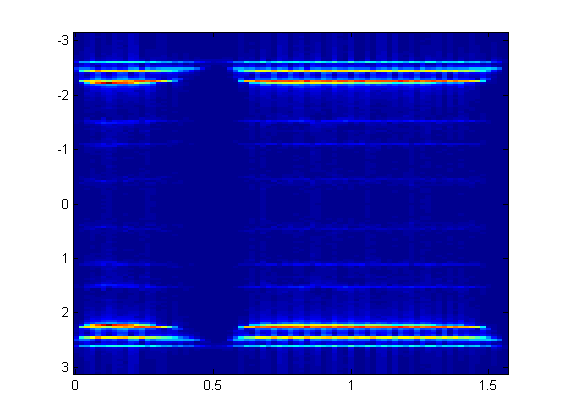
\includegraphics[scale = 0.5]{resources/labday1/timefrequentieplot.png}
\caption{Time-frequency plot.}
\label{fig:timefreq}
\end{figure}



\section{Zero padding}
Sometimes, the number of samples in a time-domain signal \textbf{x} is not very large. 
In frequency domain using the DFT, obtain the same number of samples as in time domain, and in these cases the resolution is not high.
'Zero padding' can be used to obtain a higher resolution.
Essentially, \textbf{x} (or \textbf{h}) is augmented with a lot of zeros.
After that only the DFT has to be applied to the augmented sequence. 

Firstly we use the filter in Equation \ref{eq:filter}. 
We don't apply the zero padding here (yet). 
A plot of this amplitude spectrum can be seen in Figure \ref{fig:zeropadding1}.

\begin{equation}
h = [1\quad zeros(1,5)\quad 0.9\quad zeros(1,5)\quad 0.8];
\label{eq:filter}
\end{equation}

\begin{figure}[H]
	\centering
	\setlength\figureheight{6cm}
  	\setlength\figurewidth{10cm}
	% This file was created by matlab2tikz v0.4.2.
% Copyright (c) 2008--2013, Nico Schlömer <nico.schloemer@gmail.com>
% All rights reserved.
% 
% The latest updates can be retrieved from
%   http://www.mathworks.com/matlabcentral/fileexchange/22022-matlab2tikz
% where you can also make suggestions and rate matlab2tikz.
% 
% 
% 
\begin{tikzpicture}

\begin{axis}[%
width=\figurewidth,
height=\figureheight,
scale only axis,
xmin=0,
xmax=1,
xlabel={frequency},
ymin=0,
ymax=3,
ylabel={amplitude}
]
\addplot [
color=blue,
only marks,
mark=o,
mark options={solid},
forget plot
]
table[row sep=crcr]{
0 2.7\\
0.0769230769230769 0.849045436113243\\
0.153846153846154 2.49555226711168\\
0.230769230769231 0.466566034269694\\
0.307692307692308 1.92954967807022\\
0.384615384615385 0.321656600909142\\
0.461538461538462 1.13447429946454\\
0.538461538461539 1.13447429946454\\
0.615384615384615 0.321656600909142\\
0.692307692307692 1.92954967807022\\
0.769230769230769 0.466566034269694\\
0.846153846153846 2.49555226711168\\
0.923076923076923 0.849045436113243\\
};
\end{axis}
\end{tikzpicture}%
	\caption{The amplitude spectrum with only the available samples.}
	\label{fig:zeropadding1}
\end{figure}

After plotting Figure \ref{fig:zeropadding1} we apply the 'zero padding' on the filter. 
In order to do this \textbf{h} is extended with $3\times 13 = 39$ zeros to 4 times its original length.
For the new found values we used the plot maker '+'.
In Figure \ref{fig:zeropadding2} the results of both plots are shown. 
From the figure we can conclude that we have obtained interpolation, because every 4th sample coincides with a sample from the previous plot (also see Figure \ref{fig:zeropadding1}).

\begin{figure}[H]
	\centering
	\setlength\figureheight{6cm}
  	\setlength\figurewidth{10cm}
	% This file was created by matlab2tikz v0.4.2.
% Copyright (c) 2008--2013, Nico Schlömer <nico.schloemer@gmail.com>
% All rights reserved.
% 
% The latest updates can be retrieved from
%   http://www.mathworks.com/matlabcentral/fileexchange/22022-matlab2tikz
% where you can also make suggestions and rate matlab2tikz.
% 
% 
% 
\begin{tikzpicture}

\begin{axis}[%
width=\figurewidth,
height=\figureheight,
scale only axis,
xmin=0,
xmax=1,
xlabel={frequency},
ymin=0,
ymax=3,
ylabel={amplitude}
]
\addplot [
color=blue,
only marks,
mark=o,
mark options={solid},
forget plot
]
table[row sep=crcr]{
0 2.7\\
0.0769230769230769 0.849045436113243\\
0.153846153846154 2.49555226711168\\
0.230769230769231 0.466566034269694\\
0.307692307692308 1.92954967807022\\
0.384615384615385 0.321656600909142\\
0.461538461538462 1.13447429946454\\
0.538461538461539 1.13447429946454\\
0.615384615384615 0.321656600909142\\
0.692307692307692 1.92954967807022\\
0.769230769230769 0.466566034269694\\
0.846153846153846 2.49555226711168\\
0.923076923076923 0.849045436113243\\
};
\addplot [
color=red,
solid,
forget plot
]
table[row sep=crcr]{
0 2.7\\
0.0192307692307692 2.25122933360484\\
0.0384615384615385 1.13447429946454\\
0.0576923076923077 0.205188696869487\\
0.0769230769230769 0.849045436113243\\
0.0961538461538462 0.700018622361898\\
0.115384615384615 0.321656600909142\\
0.134615384615385 1.54961370571638\\
0.153846153846154 2.49555226711168\\
0.173076923076923 2.64812785369316\\
0.192307692307692 1.92954967807022\\
0.211538461538462 0.711304609918332\\
0.230769230769231 0.466566034269694\\
0.25 0.9\\
0.269230769230769 0.466566034269694\\
0.288461538461538 0.711304609918332\\
0.307692307692308 1.92954967807022\\
0.326923076923077 2.64812785369316\\
0.346153846153846 2.49555226711168\\
0.365384615384615 1.54961370571638\\
0.384615384615385 0.321656600909142\\
0.403846153846154 0.700018622361898\\
0.423076923076923 0.849045436113243\\
0.442307692307692 0.205188696869487\\
0.461538461538462 1.13447429946454\\
0.480769230769231 2.25122933360484\\
0.5 2.7\\
0.519230769230769 2.25122933360484\\
0.538461538461538 1.13447429946454\\
0.557692307692308 0.205188696869487\\
0.576923076923077 0.849045436113243\\
0.596153846153846 0.700018622361898\\
0.615384615384615 0.321656600909142\\
0.634615384615385 1.54961370571638\\
0.653846153846154 2.49555226711168\\
0.673076923076923 2.64812785369316\\
0.692307692307692 1.92954967807022\\
0.711538461538461 0.711304609918332\\
0.730769230769231 0.466566034269694\\
0.75 0.9\\
0.769230769230769 0.466566034269694\\
0.788461538461538 0.711304609918332\\
0.807692307692308 1.92954967807022\\
0.826923076923077 2.64812785369316\\
0.846153846153846 2.49555226711168\\
0.865384615384615 1.54961370571638\\
0.884615384615385 0.321656600909142\\
0.903846153846154 0.700018622361898\\
0.923076923076923 0.849045436113243\\
0.942307692307692 0.205188696869487\\
0.961538461538461 1.13447429946454\\
0.980769230769231 2.25122933360484\\
};
\addplot [
color=blue,
only marks,
mark=+,
mark options={solid},
forget plot
]
table[row sep=crcr]{
0 2.7\\
0.0192307692307692 2.25122933360484\\
0.0384615384615385 1.13447429946454\\
0.0576923076923077 0.205188696869487\\
0.0769230769230769 0.849045436113243\\
0.0961538461538462 0.700018622361898\\
0.115384615384615 0.321656600909142\\
0.134615384615385 1.54961370571638\\
0.153846153846154 2.49555226711168\\
0.173076923076923 2.64812785369316\\
0.192307692307692 1.92954967807022\\
0.211538461538462 0.711304609918332\\
0.230769230769231 0.466566034269694\\
0.25 0.9\\
0.269230769230769 0.466566034269694\\
0.288461538461538 0.711304609918332\\
0.307692307692308 1.92954967807022\\
0.326923076923077 2.64812785369316\\
0.346153846153846 2.49555226711168\\
0.365384615384615 1.54961370571638\\
0.384615384615385 0.321656600909142\\
0.403846153846154 0.700018622361898\\
0.423076923076923 0.849045436113243\\
0.442307692307692 0.205188696869487\\
0.461538461538462 1.13447429946454\\
0.480769230769231 2.25122933360484\\
0.5 2.7\\
0.519230769230769 2.25122933360484\\
0.538461538461538 1.13447429946454\\
0.557692307692308 0.205188696869487\\
0.576923076923077 0.849045436113243\\
0.596153846153846 0.700018622361898\\
0.615384615384615 0.321656600909142\\
0.634615384615385 1.54961370571638\\
0.653846153846154 2.49555226711168\\
0.673076923076923 2.64812785369316\\
0.692307692307692 1.92954967807022\\
0.711538461538461 0.711304609918332\\
0.730769230769231 0.466566034269694\\
0.75 0.9\\
0.769230769230769 0.466566034269694\\
0.788461538461538 0.711304609918332\\
0.807692307692308 1.92954967807022\\
0.826923076923077 2.64812785369316\\
0.846153846153846 2.49555226711168\\
0.865384615384615 1.54961370571638\\
0.884615384615385 0.321656600909142\\
0.903846153846154 0.700018622361898\\
0.923076923076923 0.849045436113243\\
0.942307692307692 0.205188696869487\\
0.961538461538461 1.13447429946454\\
0.980769230769231 2.25122933360484\\
};
\end{axis}
\end{tikzpicture}%
	\caption{The amplitude spectrum.}
	\label{fig:zeropadding2}
\end{figure}


\section{The convolution property}
Here in this chapter the convolution property is demonstrated. 
This can be done by showing that Equation \ref{eq:convprop} holds.

\begin{equation}
y[n] = x[n]\star h[n] \quad \Leftrightarrow \quad Y(\omega) = X(\omega)H(\omega) 
\label{eq:convprop}
\end{equation}

To check this property we calculate $Y(\omega)$ and $X(\omega)H(\omega)$ separately and we check if both results are the same. 
We let the original signals \textbf{x} and \textbf{h} convolve with each other.
We then get the signaal $y[n]$, then, by using the DFT we get the $Y(\omega)$.\\
Now we only need to find the second part, the $X(\omega)H(\omega)$ part, respectively.
We do this by using zero padding to give both signals \textbf{x} and \textbf{h} the same length. 
If we then use DFT on our signals and use point to point multiplication, we obtain  $X(\omega)H(\omega)$.\\
Lastely we plot the absolute values in the frequencydomain. 
In Figure \ref{fig:convpro} we see two results. 
The first plot is the amplitude plot of  $X(\omega)H(\omega)$ in the frequencydomain and the second plot is the amplitude of $Y(\omega)$, also in the frequencydomain.
The plots are equal to each other, which means that convolution property holds.


\begin{figure}[h]
\centering
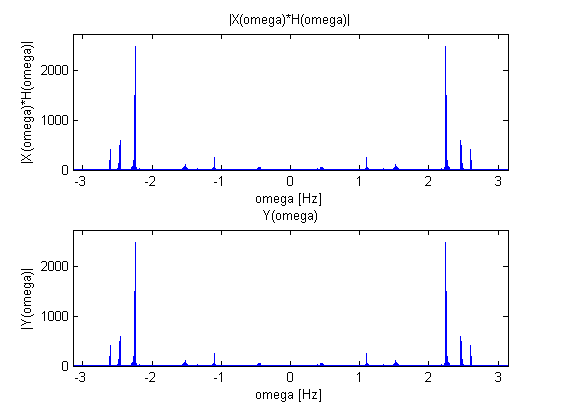
\includegraphics[scale = 1.0]{resources/labday1/theconvolutionproperty.png}
\caption{Time-frequency plot.}
\label{fig:convpro}
\end{figure}

\end{document} 